\documentclass[aspectratio = 169]{beamer}

\usepackage{../common/beamerthemedarc}
\PassOptionsToPackage{fleqn}{amsmath}
\usepackage{amsmath}
\usepackage{amssymb}
\usepackage{csquotes}
\usepackage[greek,german]{babel}
\usepackage{siunitx}
\usepackage{tabularray}
\usepackage{fontawesome5}
\usepackage{cancel}
\makeatletter
\let\ang\relax
\makeatother
\usepackage{texvc}

\DeclareSIUnit{\baud}{Bd}
\DeclareSIUnit{\dBi}{dBi}
\DeclareSIUnit{\dBm}{dBm}
\DeclareSIUnit{\dBu}{dBu}
\DeclareSIUnit{\dBV}{dbV}
\DeclareSIUnit{\dBW}{dBW}
\DeclareSIUnit{\ppm}{ppm}
\DeclareSIUnit{\pps}{pps}
\DeclareSIUnit{\CPM}{CPM}
\DeclareSIUnit{\WPM}{WPM}
\DeclareSIUnit\noop{\relax}

\definecolor{DARCgreen}{RGB}{0,155,110}
\definecolor{DARCorange}{RGB}{250,180,0}
\definecolor{DARCred}{RGB}{225,80,35}
\definecolor{DARCblue}{RGB}{0,160,220}
\definecolor{DARCgray}{RGB}{190,190,190}
\definecolor{DARClightgray}{HTML/cmyk}{e8e9e8/.11,.07,.09,0}

\definecolor{unit-title}{RGB}{155,205,185}
\definecolor{attention-title}{RGB}{255,230,170}
\definecolor{danger-title}{RGB}{245,175,150}
\definecolor{hint-title}{RGB}{185,220,245}
\definecolor{advanced-title}{RGB}{225,230,235}

\definecolor{DARCdarkblue}{RGB}{43, 103, 140}

\definecolor{r}{rgb}{0.98, 0.84, 0.65}
\definecolor{rsilver}{rgb}{0.75, 0.75, 0.75}
\definecolor{rgold}{rgb}{0.85, 0.65, 0.13}
\definecolor{rbrown}{rgb}{0.59, 0.29, 0.0}
\definecolor{rblack}{rgb}{0,0,0}
\definecolor{rred}{rgb}{0.89, 0.0, 0.13}
\definecolor{rorange}{rgb}{0.93, 0.53, 0.18}
\definecolor{ryellow}{rgb}{1.0, 0.96, 0.0}
\definecolor{rgreen}{rgb}{0.0, 0.42, 0.24}
\definecolor{rblue}{rgb}{0.06, 0.2, 0.65}
\definecolor{rviolet}{rgb}{0.56, 0.0, 1.0}
\definecolor{rgrey}{rgb}{0.33, 0.33, 0.33}
\definecolor{rwhite}{rgb}{0.96, 0.96, 0.96}

\tcbset{QSO/.style={
	enhanced,boxrule=0pt,
	frame empty,colback=DARClightgray,fontupper=\footnotesize,
	interior code={
		\fill[tcbcolback](frame.north west)to(frame.north east)to([yshift=-\ht\strutbox]interior.north east)to(interior.south east)to(interior.south west)to([yshift=-\ht\strutbox]interior.north west)--cycle;
	}
}}

\newcommand{\QSOown}[1]{\begin{tcolorbox}[
		QSO,
		leftrule=\ht\strutbox,
		right skip=.1\linewidth
]%
#1%
\end{tcolorbox}}

\newcommand{\QSOother}[1]{\begin{tcolorbox}[
		QSO,
		rightrule=\ht\strutbox,
		left skip=.1\linewidth]%
		#1%
\end{tcolorbox}}

\newenvironment{QQuestion}[6]{
    \begin{block}{#1}
        #2
        \begin{itemize}
            \item[A:] #3
            \item[B:] #4
            \item[C:] #5
            \item[D:] #6
        \end{itemize}
    \end{block}
}

\newenvironment{PQuestion}[7]{
    \begin{block}{#1}
        \begin{columns}
            \begin{column}{0.48\linewidth}
                #7
            \end{column}
            \begin{column}{0.48\linewidth}
                #2
                \begin{itemize}
                    \item[A:] #3
                    \item[B:] #4
                    \item[C:] #5
                    \item[D:] #6
                \end{itemize}
            \end{column}
        \end{columns}
    \end{block}
}

\newenvironment{question_md}[6]{
    \Question{#1}{#2}{#3}{#4}{#5}{#6}
}

\newenvironment{question2x2}[6]{
    \begin{block}{#1}
        #2
        \begin{columns}
            \begin{column}{0.48\linewidth}
                \begin{itemize}
                    \item[A:] #3
                    \item[B:] #4
                \end{itemize}
            \end{column}
            \begin{column}{0.48\linewidth}
                \begin{itemize}
                    \item[C:] #5
                    \item[D:] #6
                \end{itemize}
            \end{column}
        \end{columns}
    \end{block}
}

%\newenvironment{DARCtabular}[1]{
%    \begin{tblr}{hlines, colspec={#1}}
%}{
%    \end{tblr}
%}

\NewTblrEnviron{DARCtabular}

\SetTblrInner[DARCtabular]{
    row{odd} = {DARCblue!30},
    row{even} = {DARCblue!50},
    row{1} = {bg=DARCblue, fg=white, font=\bfseries}
}

\SetTblrOuter[DARCtabular]{
    baseline=B
}

\PassOptionsToPackage{locale=DE}{siunitx}
\PassOptionsToPackage{straightvoltages, europeanresistors, european inductor}{circuitikz}

\usepackage[locale=DE]{siunitx}
\usepackage{ifthen}
\usepackage{mathtools}
\usepackage{unicode-math}
\setmathfont{Libertinus Math}

\usepackage{circuitikz}
\makeatletter
\let\empty\relax
\makeatother
\usepackage{pgfplots}
\usepackage{pgfmath}
\usepackage{pgfplotstable}

\usepackage{etoolbox}
\usepackage{xcolor}
\usepackage{MnSymbol}

\usepackage{wasysym}
\usepackage{tikz-dimline}
\AtBeginDocument{\RenewCommandCopy\qty\SI} % Fix um qty doppeldefinition zu vermeiden 
\usepackage{tikz-3dplot}
%\usepackage{filecontents}% removed as obsolete

%TODO remove?
\usepackage{varwidth}
\usepackage{pgf-spectra}
\usepgfspectralibrary{pgfplots}

% TODO
% hier mal hart forciert, weil if ggf nicht geht?
% define colormap and check if cmyk is enforced
%\def\test#1{cmyk}
%\ifx\XC@tgt@mod\test
%	\pgfplotsset{colormap={slategraywhite}{cmyk=(0,0,0,.8) cmyk=(0,0,0,0)}}
%\else
	\pgfplotsset{colormap={slategraywhite}{rgb255=(50,50,50) rgb255=(255,255,255)}}
%\fi


\usetikzlibrary{math,perspective,intersections,arrows,arrows.meta,positioning,calc,shapes.symbols,decorations.pathmorphing,patterns,shapes.geometric,matrix,3d,backgrounds,babel,pgfplots.polar,decorations.pathreplacing,calligraphy,decorations.text,svg.path,optics}
\usepgfplotslibrary{fillbetween}
\pgfplotsset{compat=1.18}
\DeclareSIUnit{\baud}{Bd}

\sisetup{
    range-phrase=--,
    range-units=single
}

\usepackage[euler]{textgreek}

% Setze die Enden der optischen Pfeile etc. auf 60 grad:
\ctikzset{
	opto end arrow={Triangle[angle'=60]},
	tunable end arrow={Triangle}
}

% Grundsätzlich alle Pfeile als Triangle TODO, danach suchen und dann loeschen!
\tikzset{
    myarrow/.style={-Triangle}
}
\ctikzset{
    resistor=european,
    voltage=straight
}

\tikzstyle{digitalNumber}=[draw=DARCgray, fill=white, minimum width=0.5, minimum height=0.5, rounded corners=1, font=\bfseries]

% Gekritzelte Linie (Bild 315)
\pgfdeclaredecoration{penciline}{initial}{
	\state{initial}[width=+\pgfdecoratedinputsegmentremainingdistance,
	auto corner on length=1mm,]{
		\pgfpathcurveto%
		{% From
			\pgfqpoint{\pgfdecoratedinputsegmentremainingdistance}
			{\pgfdecorationsegmentamplitude}
		}
		{%  Control 1
			\pgfmathrand
			\pgfpointadd{\pgfqpoint{\pgfdecoratedinputsegmentremainingdistance}{0pt}}
			{\pgfqpoint{-\pgfdecorationsegmentaspect
					\pgfdecoratedinputsegmentremainingdistance}%
				{\pgfmathresult\pgfdecorationsegmentamplitude}
			}
		}
		{%TO
			\pgfpointadd{\pgfpointdecoratedinputsegmentlast}{\pgfpoint{1pt}{1pt}}
		}
	}
	\state{final}{}
}

% Bandplan bänder in Bild 750 und 749
\let\band\relax% conflict… requires cleanup … \providecommand? 
\newcommand{\band}[7]{%
    \draw[draw=red] (-5,#1) rectangle (5,#2);
    \draw ( 40,#1) node[right,rotate=0, text=red](){\footnotesize\textbf{\SI{#6}{#7}}};
    \draw ( 20,#1) node[rotate=0](){\footnotesize\SI{#3}{#5}};
    \draw (-20,#2) node[rotate=0](){\footnotesize\SI{#4}{#5}};
}

\let\bandB\relax% conflict… requires cleanup … \providecommand? 
\newcommand{\bandB}[7]{%
    \draw[draw=red] (-5,#1) rectangle (5,#2);
    \draw ( 40,#1) node[right,rotate=0, text=red](){\footnotesize\textbf{\SI{#6}{#7}}};
    \draw ( 20,#1) node[rotate=0,above](){\footnotesize\SI{#3}{#5}};
    \draw (-20,#2) node[rotate=0,above](){\footnotesize\SI{#4}{#5}};
}

\newcommand{\bandC}[7]{%
    \draw[draw=red] (#1,-5) rectangle (#2,5);
    \draw (#1, 65.0) node[rotate=-90, text=red](){\footnotesize\textbf{\SI{#6}{#7}}};
    \draw (#1, 27.5) node[rotate=-90](){\footnotesize\SI{#3}{#5}};
    \draw (#2,-27.5) node[rotate=-90](){\footnotesize\SI{#4}{#5}};
}

\newcommand{\bandD}[5]{%
    \draw[draw=red] (#1,-5) rectangle (#2,5);
    \draw (#1+50000000, 27.5) node[rotate=-90](){\footnotesize\SI{#3}{#5}};
    \draw (#2+50000000,-27.5) node[rotate=-90](){\footnotesize\SI{#4}{#5}};
}

% Symbol für das Gleichstrom
\newcommand{\textdirectcurrent}{%
  \settowidth{\dimen0}{$=$}%
  \vbox to .85ex {\offinterlineskip
    \hbox to \dimen0{\leaders\hrule\hfill}
    \vskip.35ex
    \hbox to \dimen0{%
      \leaders\hrule\hskip.2\dimen0\hfill
      \leaders\hrule\hskip.2\dimen0\hfill
      \leaders\hrule\hskip.2\dimen0
    }
    \vfill
  }%
}
\newcommand{\mathdirectcurrent}{\mathrel{\textdirectcurrent}}

% Zum Messen von Abständen
\makeatletter
\newcommand{\Distance}[3]{% from https://tex.stackexchange.com/q/56353/121799
	\tikz@scan@one@point\pgfutil@firstofone($#1-#2$)\relax  
	\pgfmathsetmacro{#3}{round(0.99626*veclen(\the\pgf@x,\the\pgf@y)/0.0283465)/1000}
}
\makeatother

% Bemaßung zeichnen:
\NewDocumentCommand\DARCmeasure{O{black} O{middle} m m m m m}{% 1:[color], 2:[top], 3:start, 4:end, 5:shift, 6:rotate, 7:text
    \path($(#3)+(#5)$) coordinate(start);
    \path($(#4)+(#5)$) coordinate(end);
    \ifthenelse{\equal{#2}{top}}{
        \draw ($(start)!0.5!(end)$) coordinate(middle);
        \node[rotate=#6, anchor=south] (text) at (middle) {\textcolor{#1}{#7}};
        \draw[draw=#1, |Triangle-] (start) -- (middle);
        \draw[draw=#1, |Triangle-] (end) -- (middle);
    }{
        \node[rotate=#6] (text) at ($(start)!0.5!(end)$) {\textcolor{#1}{#7}};
        \draw[draw=#1, |Triangle-] (start) -- (text.west);
        \draw[draw=#1, |Triangle-] (end) -- (text.east);
    }
}

% Magic von Marei zur Skalierung der Bilder
\makeatletter
\ExplSyntaxOn
\box_new:N \l_ptxcd_image_box

\cs_if_exist:NF \if@DARCinQuestion {\newif\if@DARCinQuestion}

\fp_if_exist:NF \l_ptxcd_tmp_fp {\fp_new:N \l_ptxcd_tmp_fp}
\fp_set:Nn \l_ptxcd_tmp_fp  {1}

\int_new:N \g_DARC_image_fail_int
\seq_new:N \g__DARC_image_fail_seq
\dim_new:N \l__DARC_image_width_dim
\box_new:N \l_ptxcd_image_orig_box

\newcommand*{\getDarcImageFactor}{\fp_use:N  \l_ptxcd_tmp_fp}



\NewDocumentCommand{\DARCimageOnly}{smm}{
	\setmathfont{Libertinus Math}
	 \ptxcd_image_autoscale_setup:nnn {#1} {#2} {#3}
		\usepackage{geometry}
        \usepackage{}
	\geometry{paperwidth=\box_wd:N  \l_ptxcd_image_box, paperheight=\box_ht_plus_dp:N  \l_ptxcd_image_box,margin=0pt}
	\pagestyle{empty}
	\setlength{\topskip}{0pt}% necessary because otherwhise \topskip could exceed \paperheight
	\begin{document}
		\box_use:N \l_ptxcd_image_box
	\end{document}
}

\seq_new:N  \g__ptxcd_image_size_seq
\prop_new:N \g__ptxcd_image_size_cache_prop
\bool_new:N \l__ptxcd_disable_autoscale_bool
\newcommand*{\disableDARCautoscale}{\bool_set_true:N  \l__ptxcd_disable_autoscale_bool}

\cs_new:Nn \ptxcd_image_autoscale_setup:nnn {
	\prop_if_in:NnTF \g__ptxcd_image_size_cache_prop {#2} {
			\fp_set:Nn \l_ptxcd_tmp_fp {\prop_item:Nn \g__ptxcd_image_size_cache_prop {#2}}
			\hbox_gset:Nn \l_ptxcd_image_box {
				\tikzset{x=\fp_use:N \l_ptxcd_tmp_fp cm,y=\fp_use:N \l_ptxcd_tmp_fp cm}
				\file_if_exist_input:n {img/#2}%
				\ifvmode\else\unskip\fi
			}
		\seq_gput_right:Nx \g__ptxcd_image_size_seq {#2=\prop_item:Nn \g__ptxcd_image_size_cache_prop {#2}}
	} {
		\hbox_gset:Nn \l_ptxcd_image_orig_box {
			\file_if_exist_input:n {img/#3}%
			\ifvmode\else\unskip\fi%
		}
		\bool_if:NT \l__ptxcd_disable_autoscale_bool \use_iii:nnnn
		\IfBooleanTF{#1}{
			\box_gset_eq:NN \l_ptxcd_image_box \l_ptxcd_image_orig_box
		} {
			\dim_compare:nNnTF {\box_wd:N \l_ptxcd_image_orig_box} = {\c_zero_dim} {
				\fp_set:Nn  \l_ptxcd_tmp_fp {1}
			} {
				\if@DARCinQuestion
					\dim_compare:nTF {#2 =\linewidth} {
						\dim_set:Nn  \l__DARC_image_width_dim {\columnwidth}
					} {
						\dim_set:Nn  \l__DARC_image_width_dim {#2}
					}
				\else
					\dim_set:Nn  \l__DARC_image_width_dim {#2}
				\fi
				\fp_set:Nn \l_ptxcd_tmp_fp {\dim_to_decimal_in_unit:nn {\l__DARC_image_width_dim} {\box_wd:N \l_ptxcd_image_orig_box}}
				\hbox_gset:Nn \l_ptxcd_image_box {
					\tikzset{x=\fp_use:N \l_ptxcd_tmp_fp cm,y=\fp_use:N \l_ptxcd_tmp_fp cm}
					\file_if_exist_input:n {img/#3}%
					\ifvmode\else\unskip\fi
				}
				\bool_lazy_and:nnT
					{ \dim_compare_p:nNn {\box_wd:N \l_ptxcd_image_box} < {\l__DARC_image_width_dim  -1em} }
					{ ! \dim_compare_p:nNn {\box_wd:N \l_ptxcd_image_box} = {\box_wd:N \l_ptxcd_image_orig_box}}
				{
					\fp_set:Nn \l_ptxcd_tmp_fp { 1 + \dim_to_decimal_in_unit:nn {\l__DARC_image_width_dim- \box_wd:N \l_ptxcd_image_orig_box} {\box_wd:N \l_ptxcd_image_box - \box_wd:N \l_ptxcd_image_orig_box} * (\l_ptxcd_tmp_fp  -1)}
					\hbox_gset:Nn \l_ptxcd_image_box {
						\tikzset{x=\fp_use:N \l_ptxcd_tmp_fp cm,y=\fp_use:N \l_ptxcd_tmp_fp cm}
						\file_if_exist_input:n {img/#3}%
						\ifvmode\else\unskip\fi
					}
				}
				\dim_compare:nNnTF  {\box_wd:N \l_ptxcd_image_box} = {\box_wd:N \l_ptxcd_image_orig_box} {
					\seq_gput_right:Nx \g__ptxcd_image_size_seq {#3=1}
				}{
					\seq_gput_right:Nx \g__ptxcd_image_size_seq {#3=\fp_use:N \l_ptxcd_tmp_fp}
				}
			}
		}
	}
}

\newcommand*{\DARCimageCache}[1]{
	\prop_gset_from_keyval:Nn \g__ptxcd_image_size_cache_prop {#1}
}

\hook_gput_code:nnn {enddocument/afterlastpage}{write-DARCimage-size-cache}{
	\iow_now:Ne \@auxout {
		\exp_not:N \DARCimageCache{
			\seq_use:Nn  \g__ptxcd_image_size_seq {,}
		}
	}
}

\NewDocumentCommand{\DARCimage}{sO{Bild~zur~Prüfungsfrage~\l_ptxcd_question_tl}mm}{
	\par\smallskip
	\begingroup
		\ptxcd_image_autoscale_setup:nnn {#1} {#3} {#4}
		\dim_compare:nNnTF {\box_wd:N \l_ptxcd_image_box} > {\linewidth}
		{
			\makebox[\linewidth][r]{\box_use:N \l_ptxcd_image_box}
		} {
			\makebox[\linewidth][c]{\box_use:N \l_ptxcd_image_box}
		}
	\endgroup
}
\ExplSyntaxOff
\makeatother

% Neue TL, wird bald in einem zukünftigen circuittikz sein: 
% https://github.com/circuitikz/circuitikz/issues/694
\makeatletter
\newif\ifpgf@circ@bare@tline
\ctikzset{bipoles/tline/bare/.is if=pgf@circ@bare@tline}
\pgfcircdeclarebipolescaled{RF}
{
\savedmacro{\recessright}{\edef\recessright{\ifpgf@circ@bare@tline -0.4\else 0.0\fi}}
\anchor{center right}{\northeast \advance\pgf@x by -0.4\pgf@y\pgf@y=0pt}
\anchor{top right}{\northeast \advance\pgf@x by -0.4\pgf@y}
\anchor{bottom right}{\northeast \advance\pgf@x by -0.4\pgf@y\pgf@y=-\pgf@y}
\anchor{center left}{\northeast \advance\pgf@x by -0.4\pgf@y\pgf@x=-\pgf@x\pgf@y=0pt}
\anchor{top left}{\northeast \advance\pgf@x by -0.4\pgf@y\pgf@x=-\pgf@x}
\anchor{bottom left}{\northeast \advance\pgf@x by -0.4\pgf@y\pgf@x=-\pgf@x\pgf@y=-\pgf@y}
\anchor{right}{\northeast \advance\pgf@x by \recessright\pgf@y\pgf@y=0pt}
}
{\ctikzvalof{bipoles/tline/height}}
{tline}
{\ctikzvalof{bipoles/tline/height}}
{\ctikzvalof{bipoles/tline/width}}
{
\pgf@circ@res@step=.4\pgf@circ@res@up % the size of the ellipsis is proportional to the height
\pgfscope
\pgf@circ@setlinewidth{bipoles}{\pgfstartlinewidth}
\pgfpathmoveto{\pgfpoint{\pgf@circ@res@right-\pgf@circ@res@step}{\pgf@circ@res@up}}
\pgfpathlineto{\pgfpoint{\pgf@circ@res@left+\pgf@circ@res@step}{\pgf@circ@res@up}}
\pgfpatharc{-90}{90}{-\pgf@circ@res@step and -\pgf@circ@res@up}
\pgfpathlineto{\pgfpoint{\pgf@circ@res@right-\pgf@circ@res@step}{\pgf@circ@res@down}}
\pgfpatharc{-90}{90}{\pgf@circ@res@step and \pgf@circ@res@up}
\pgf@circ@draworfill
\pgfpathmoveto{\pgfpoint{\pgf@circ@res@right-\pgf@circ@res@step}{\pgf@circ@res@up}}
\pgfpatharc{-90}{90}{-\pgf@circ@res@step and -\pgf@circ@res@up}
\pgfusepath{stroke}
\endpgfscope
\ifpgf@circ@bare@tline\else
\pgfsetlinewidth{\pgfstartlinewidth}
\pgfpathmoveto{\pgfpoint{\pgf@circ@res@right-\pgf@circ@res@step}{0pt}}
\pgfpathlineto{\pgfpoint{\pgf@circ@res@right}{0pt}}
\pgfusepath{stroke}
\fi
}
\makeatother

% Neues mikrofon, wird irgendwann teil von circuit tikzi und kann dann hier
% gelöscht werden: https://github.com/circuitikz/circuitikz/issues/689
% <
\makeatletter
\ctikzset{bipoles/tlmic/height/.initial=.5}
\ctikzset{bipoles/tlmic/depth/.initial=.5}
\ctikzset{bipoles/tlmic/width/.initial=.5}%
\pgfcircdeclarebipolescaled{misc}
{}
{\ctikzvalof{bipoles/tlmic/depth}}
{tlmic}
{\ctikzvalof{bipoles/tlmic/height}}
{\ctikzvalof{bipoles/tlmic/width}}{

    \pgf@circ@setlinewidth{bipoles}{\pgfstartlinewidth}
    \pgfpathcircle{\pgfpoint{0pt}{0pt}}{\pgf@circ@res@up}
    \pgf@circ@draworfill
    \pgfpathmoveto{\pgfpoint{\pgf@circ@res@left}{\pgf@circ@res@up}}
    \pgfpathlineto{\pgfpoint{\pgf@circ@res@right}{\pgf@circ@res@up}}
    \pgfusepath{draw}
}
\pgfcirc@activate@bipole@simple{l}{tlmic}

\makeatother
% />

% Power Plug
\makeatletter
\ctikzset{bipoles/plug/height/.initial=.5}
\ctikzset{bipoles/plug/width/.initial=.5}%
\pgfcircdeclarebipolescaled{misc}
{}
{\ctikzvalof{bipoles/plug/height}}
{plug}
{\ctikzvalof{bipoles/plug/height}}
{\ctikzvalof{bipoles/plug/width}}{

    %\pgf@circ@setlinewidth{bipoles}{\pgfstartlinewidth}
    \pgfpathcircle{\pgfpoint{0pt}{0pt}}{\pgf@circ@res@up}
	\pgfusepath{fill}
    %\pgfpathmoveto{\pgfpoint{\pgf@circ@res@left}{\pgf@circ@res@up}}
    %\pgfpathlineto{\pgfpoint{\pgf@circ@res@right}{\pgf@circ@res@up}}
    %\pgfusepath{draw}
	% Plus:
	\color{black} 
	\pgfsetstrokecolor{black} 
	\pgfpathrectangle{\pgfpoint{0.0\pgf@circ@res@step}{-0.1\pgf@circ@res@step}}{\pgfpoint{-0.2\pgf@circ@res@step}{+0.1\pgf@circ@res@step}}%
	\pgfusepath{fill}
}
\pgfcirc@activate@bipole@simple{l}{plug}
\makeatother

%% bgenerator und bgeneratorshape block
% Eine submission nach circuittikz wurde durchgeführt: 
% https://github.com/circuitikz/circuitikz/pull/693
% <
\makeatletter
%
\def\pgfcirc@twoport@draw@narrowsine#1{% #1 -> y shift
    \pgfscope
        \pgfsetlinewidth{\pgfstartlinewidth}
        \pgftransformyshift{#1\pgf@circ@res@step}
        \pgfpathmoveto{\pgfpoint{.125\pgf@circ@res@step}{0\pgf@circ@res@step}}
        \pgfpathsine{\pgfpoint{.125\pgf@circ@res@step}{.125\pgf@circ@res@step}}
        \pgfpathcosine{\pgfpoint{.125\pgf@circ@res@step}{-.125\pgf@circ@res@step}}
        \pgfpathsine{\pgfpoint{.125\pgf@circ@res@step}{-.125\pgf@circ@res@step}}
        \pgfpathcosine{\pgfpoint{.125\pgf@circ@res@step}{.125\pgf@circ@res@step}}
        \pgfusepath{draw}
    \endpgfscope
}
%
\ctikzset{bipoles/bgenerator/width/.initial=.7}
\pgfcirc@define@twoports{blocks}
{}
{\ctikzvalof{bipoles/bgenerator/width}}
{bgenerator}
{\ctikzvalof{bipoles/bgenerator/width}}
{\ctikzvalof{bipoles/bgenerator/width}}
{
    \pgfcirc@twoport@draw@narrowsine{0.25}{0}
    \pgfcirc@twoport@draw@narrowsine{0.0}{0}
    \pgfcirc@twoport@draw@narrowsine{-0.25}{0}
    \pgftext[x=0.45\pgf@circ@res@left]{\ctikzvalof{bipoles/twoport/text}}
}
\pgfcirc@activate@bipole@simple{l}{bgenerator}
\makeatother
%>

%Q-Generator TODO: Update pull request
\makeatletter
%
\ctikzset{bipoles/qgenerator/width/.initial=.7}
\pgfcirc@define@twoports{blocks}
{}
{\ctikzvalof{bipoles/qgenerator/width}}
{qgenerator}
{\ctikzvalof{bipoles/qgenerator/width}}
{\ctikzvalof{bipoles/qgenerator/width}}
{
    \pgfcirc@twoport@draw@narrowsine{0.45}{0}
    \pgfcirc@twoport@draw@narrowsine{0.20}{0}
    \pgfcirc@twoport@draw@narrowsine{-0.05}{0}
    \pgftext[x=0.45\pgf@circ@res@left,y=0.25\pgf@circ@res@up]{\ctikzvalof{bipoles/twoport/text}}
	\pgfpathmoveto{\pgfpoint{-0.7\pgf@circ@res@step}{-0.35\pgf@circ@res@step}} 
	\pgfpathlineto{\pgfpoint{ 0.7\pgf@circ@res@step}{-0.35\pgf@circ@res@step}} 
    \pgfusepath{draw}
	\pgfpathrectangle{\pgfpoint{-0.7\pgf@circ@res@step}{-0.7\pgf@circ@res@step}}{\pgfpoint{1.4\pgf@circ@res@step}{0.2\pgf@circ@res@step}} 
    \pgfusepath{draw}
	\pgfpathmoveto{\pgfpoint{-0.7\pgf@circ@res@step}{-0.85\pgf@circ@res@step}} 
	\pgfpathlineto{\pgfpoint{ 0.7\pgf@circ@res@step}{-0.85\pgf@circ@res@step}} 
    \pgfusepath{draw}
}
\pgfcirc@activate@bipole@simple{l}{qgenerator}
\makeatother

%Clock-Generator TODO: Add to pull request
\makeatletter
%
\ctikzset{bipoles/cgenerator/width/.initial=.7}
\pgfcirc@define@twoports{blocks}
{}
{\ctikzvalof{bipoles/cgenerator/width}}
{cgenerator}
{\ctikzvalof{bipoles/cgenerator/width}}
{\ctikzvalof{bipoles/cgenerator/width}}
{
	\pgfpathmoveto{\pgfpoint{-0.70\pgf@circ@res@step}{-0.35\pgf@circ@res@step}} 
	\pgfpathlineto{\pgfpoint{-0.42\pgf@circ@res@step}{-0.35\pgf@circ@res@step}} 
	\pgfpathlineto{\pgfpoint{-0.42\pgf@circ@res@step}{+0.35\pgf@circ@res@step}} 
	\pgfpathlineto{\pgfpoint{-0.14\pgf@circ@res@step}{+0.35\pgf@circ@res@step}} 
	\pgfpathlineto{\pgfpoint{-0.14\pgf@circ@res@step}{-0.35\pgf@circ@res@step}} 
	\pgfpathlineto{\pgfpoint{+0.14\pgf@circ@res@step}{-0.35\pgf@circ@res@step}} 
	\pgfpathlineto{\pgfpoint{+0.14\pgf@circ@res@step}{+0.35\pgf@circ@res@step}} 
	\pgfpathlineto{\pgfpoint{+0.42\pgf@circ@res@step}{+0.35\pgf@circ@res@step}} 
	\pgfpathlineto{\pgfpoint{+0.42\pgf@circ@res@step}{-0.35\pgf@circ@res@step}} 
	\pgfpathlineto{\pgfpoint{+0.70\pgf@circ@res@step}{-0.35\pgf@circ@res@step}} 
    \pgfusepath{draw}
}
\pgfcirc@activate@bipole@simple{l}{cgenerator}
\makeatother

%Sine Table: TODO in pullrequest packen
\makeatletter
%
\ctikzset{bipoles/sinetable/width/.initial=.7}
\pgfcirc@define@twoports{blocks}
{}
{\ctikzvalof{bipoles/sinetable/width}}
{sinetable}
{\ctikzvalof{bipoles/sinetable/width}}
{\ctikzvalof{bipoles/sinetable/width}}
{
    \pgfcirc@twoport@draw@sine{0.0}{0}
    \pgfcirc@set@arrows{tunable}{}{latex}
	\pgfpathmoveto{\pgfpoint{-0.70\pgf@circ@res@step}{-0.70\pgf@circ@res@step}} 
	\pgfpathlineto{\pgfpoint{+0.70\pgf@circ@res@step}{-0.70\pgf@circ@res@step}} 
    \pgfusepath{draw}
	\pgfpathmoveto{\pgfpoint{-0.70\pgf@circ@res@step}{-0.70\pgf@circ@res@step}} 
	\pgfpathlineto{\pgfpoint{-0.70\pgf@circ@res@step}{+0.70\pgf@circ@res@step}} 
    \pgfusepath{draw}
}
\pgfcirc@activate@bipole@simple{l}{sinetable}
\makeatother

%Sine Table: TODO in pullrequest packen
\makeatletter
%
\ctikzset{bipoles/register/width/.initial=.7}
\pgfcirc@define@twoports{blocks}
{
	\savedanchor\northwest{
		\pgfmathsetlength{\pgf@circ@scaled@Rlen}{\ctikzvalof{\ctikzclass/scale}\pgf@circ@Rlen}
		\pgf@y=\ctikzvalof{bipoles/twoport/width}\pgf@circ@scaled@Rlen
		\pgf@y=.5\pgf@y
		\pgf@x=-\ctikzvalof{bipoles/twoport/width}\pgf@circ@scaled@Rlen
		\pgf@x=.5\pgf@x
	}
	\anchor{clk}{\northwest\pgf@y=0.5\pgf@y}
}
{\ctikzvalof{bipoles/register/width}}
{register}
{\ctikzvalof{bipoles/register/width}}
{\ctikzvalof{bipoles/register/width}}
{
	\pgfpathmoveto{\pgfpoint{-1.00\pgf@circ@res@step}{+0.70\pgf@circ@res@step}} 
	\pgfpathlineto{\pgfpoint{-0.60\pgf@circ@res@step}{+0.50\pgf@circ@res@step}} 
	\pgfpathlineto{\pgfpoint{-1.00\pgf@circ@res@step}{+0.30\pgf@circ@res@step}} 
    \pgfusepath{draw}
}
\pgfcirc@activate@bipole@simple{l}{register}
\makeatother

%% Bias-T
% TODO, add to pull request
\makeatletter
\ctikzset{bipoles/biast/width/.initial=.7}
\pgfcirc@define@twoports{blocks}
{}
{\ctikzvalof{bipoles/biast/width}}
{biast}
{\ctikzvalof{bipoles/biast/width}}
{\ctikzvalof{bipoles/biast/width}}
{
	\pgfpathmoveto{\pgfpoint{-0.80\pgf@circ@res@step}{-0.50\pgf@circ@res@step}} % Line to Plate 1
	\pgfpathlineto{\pgfpoint{-0.50\pgf@circ@res@step}{-0.50\pgf@circ@res@step}} 
	\pgfpathmoveto{\pgfpoint{-0.50\pgf@circ@res@step}{-0.50\pgf@circ@res@step}} % Plate 1
	\pgfpathlineto{\pgfpoint{-0.50\pgf@circ@res@step}{-0.20\pgf@circ@res@step}} 
	\pgfpathmoveto{\pgfpoint{-0.50\pgf@circ@res@step}{-0.50\pgf@circ@res@step}} 
	\pgfpathlineto{\pgfpoint{-0.50\pgf@circ@res@step}{-0.80\pgf@circ@res@step}} 
	\pgfpathmoveto{\pgfpoint{-0.30\pgf@circ@res@step}{-0.50\pgf@circ@res@step}} % Plate 1
	\pgfpathlineto{\pgfpoint{-0.30\pgf@circ@res@step}{-0.20\pgf@circ@res@step}} 
	\pgfpathmoveto{\pgfpoint{-0.30\pgf@circ@res@step}{-0.50\pgf@circ@res@step}} 
	\pgfpathlineto{\pgfpoint{-0.30\pgf@circ@res@step}{-0.80\pgf@circ@res@step}}
	\pgfpathmoveto{\pgfpoint{-0.30\pgf@circ@res@step}{-0.50\pgf@circ@res@step}} % Line to Center
	\pgfpathlineto{\pgfpoint{ 0.00\pgf@circ@res@step}{-0.50\pgf@circ@res@step}} 
    \pgfusepath{draw}
    \pgfpathcircle{\pgfpoint{ 0.00\pgf@circ@res@step}{-0.50\pgf@circ@res@step}}{0.075\pgf@circ@res@step}
    \pgfusepath{fill}
	\pgfpathmoveto{\pgfpoint{ 0.00\pgf@circ@res@step}{-0.50\pgf@circ@res@step}} % Line to Right
	\pgfpathlineto{\pgfpoint{ 0.80\pgf@circ@res@step}{-0.50\pgf@circ@res@step}} 
    \pgfusepath{draw}
	\pgfpathmoveto{\pgfpoint{ 0.00\pgf@circ@res@step}{-0.50\pgf@circ@res@step}} % Line to Coils
	\pgfpathlineto{\pgfpoint{ 0.00\pgf@circ@res@step}{-0.20\pgf@circ@res@step}} 
    \pgfusepath{draw}
	\pgfpathmoveto{\pgfpoint{ 0.00\pgf@circ@res@step}{-0.20\pgf@circ@res@step}} % Arc1
	\pgfpatharc{-90}{90}{0.09\pgf@circ@res@step}
	\pgfpathmoveto{\pgfpoint{ 0.00\pgf@circ@res@step}{-0.02\pgf@circ@res@step}} % Arc2
	\pgfpatharc{-90}{90}{0.09\pgf@circ@res@step}
	\pgfpathmoveto{\pgfpoint{ 0.00\pgf@circ@res@step}{+0.16\pgf@circ@res@step}} % Arc3
	\pgfpatharc{-90}{90}{0.09\pgf@circ@res@step}
	\pgfpathmoveto{\pgfpoint{ 0.00\pgf@circ@res@step}{+0.36\pgf@circ@res@step}} % Arc4
	\pgfpatharc{-90}{90}{0.09\pgf@circ@res@step}
	\pgfusepath{draw}
	\pgfpathmoveto{\pgfpoint{ 0.00\pgf@circ@res@step}{+0.52\pgf@circ@res@step}} % Line to Coils
	\pgfpathlineto{\pgfpoint{ 0.00\pgf@circ@res@step}{+0.80\pgf@circ@res@step}} 
	\pgfusepath{draw}
}
\pgfcirc@activate@bipole@simple{l}{biast}
\makeatother

%% variable allpass filter
% Eine submission nach circuittikz wurde durchgeführt: 
% https://github.com/circuitikz/circuitikz/pull/693
\makeatletter
\ctikzset{bipoles/vallpass/width/.initial=.7}
\pgfcirc@define@twoports{blocks}
{}
{\ctikzvalof{bipoles/vallpass/width}}
{vallpass}
{\ctikzvalof{bipoles/vallpass/width}}
{\ctikzvalof{bipoles/vallpass/width}}
{
    \pgfcirc@twoport@draw@sine{0.5}{0}
    \pgfcirc@twoport@draw@sine{0.0}{0}
    \pgfcirc@twoport@draw@sine{-0.5}{0}
    \pgfcirc@set@arrows{tunable}{}{latex}
    \pgfpathmoveto{\pgfpoint{0.7\pgf@circ@res@left}{0.5\pgf@circ@res@down}}
    \pgfpathlineto{\pgfpoint{0.7\pgf@circ@res@right}{0.8\pgf@circ@res@up}}
    \pgfusepath{draw}
}
\pgfcirc@activate@bipole@simple{l}{vallpass}
\makeatother

%% bgenerator und bgeneratorshape block
% <
\makeatletter
%
\ctikzset{bipoles/ngenerator/width/.initial=.7}
\pgfcirc@define@twoports{blocks}
{}
{\ctikzvalof{bipoles/ngenerator/width}}
{ngenerator}
{\ctikzvalof{bipoles/ngenerator/width}}
{\ctikzvalof{bipoles/ngenerator/width}}
{
    \pgfcirc@twoport@draw@sine{0.5}{0}
    \pgftext[y=-0.35\pgf@circ@res@up]{\ctikzvalof{bipoles/twoport/text}}
}
\pgfcirc@activate@bipole@simple{l}{ngenerator}
\makeatother
%>

% Camera
% has to be commited to PR
\makeatletter
\ctikzset{bipoles/camera/height/.initial=1.2}
\ctikzset{bipoles/camera/depth/.initial=.3}
\ctikzset{bipoles/camera/width/.initial=.4}
\pgfcircdeclarebipolescaled{misc}
{}
{\ctikzvalof{bipoles/camera/depth}}
{camera}
{\ctikzvalof{bipoles/camera/height}}
{\ctikzvalof{bipoles/camera/width}}{
    \pgfpathrectanglecorners{\pgfpoint{\pgf@circ@res@left}{.7\pgf@circ@res@up}}
    {\pgfpoint{\pgf@circ@res@right}{\pgf@circ@res@down}}
    \pgfpathmoveto{\pgfpoint{0.5\pgf@circ@res@left}{.7\pgf@circ@res@up}}
    \pgfpathlineto{\pgfpoint{0.8\pgf@circ@res@left}{\pgf@circ@res@up}}
    \pgfpathlineto{\pgfpoint{0.8\pgf@circ@res@right}{\pgf@circ@res@up}}
    \pgfpathlineto{\pgfpoint{0.5\pgf@circ@res@right}{.7\pgf@circ@res@up}}
    \pgfpathclose
    \pgf@circ@setlinewidth{bipoles}{\pgfstartlinewidth}
    \pgf@circ@draworfill
}
\pgfcirc@activate@bipole@simple{l}{camera}

\makeatother

% TRX
% has to be commited to PR
\makeatletter
\ctikzset{bipoles/trx/width/.initial=1}
\ctikzset{bipoles/trx/height/.initial=.4}
\pgfcirc@define@twoports{blocks}
{
	\anchor{plus}{\northeast \advance\pgf@y by -0.2\pgf@x\pgf@x=-\pgf@x}
	\anchor{minus}{\northeast \advance\pgf@y by -0.2\pgf@x\pgf@x=-\pgf@x\pgf@y=-\pgf@y}
}
{\ctikzvalof{bipoles/trx/height}}
{trx}
{\ctikzvalof{bipoles/trx/height}}
{\ctikzvalof{bipoles/trx/width}}
{
	% VFO-Rad:
	\pgfpathcircle{\pgfpoint{0.60\pgf@circ@res@step}{0.00\pgf@circ@res@step}}{0.25\pgf@circ@res@step}
	\pgfpathcircle{\pgfpoint{0.68\pgf@circ@res@step}{0.10\pgf@circ@res@step}}{0.06\pgf@circ@res@step}
	% Lautstärke und Rauschsperre:
	\pgfpathcircle{\pgfpoint{-0.8\pgf@circ@res@step}{+0.15\pgf@circ@res@step}}{0.1\pgf@circ@res@step}
	\pgfpathcircle{\pgfpoint{-0.8\pgf@circ@res@step}{-0.15\pgf@circ@res@step}}{0.1\pgf@circ@res@step}
	% Bildschirm:
	\pgfpathrectangle{\pgfpoint{-0.55\pgf@circ@res@step}{-0.25\pgf@circ@res@step}}{\pgfpoint{+0.75\pgf@circ@res@step}{+0.5\pgf@circ@res@step}}%
    \pgfusepath{draw}
}
\pgfcirc@activate@bipole@simple{l}{trx}
\makeatother

% SWR
% has to be commited to PR
\makeatletter
\ctikzset{bipoles/swr/width/.initial=0.6}
\ctikzset{bipoles/swr/height/.initial=.4}
\pgfcirc@define@twoports{blocks}
{}
{\ctikzvalof{bipoles/swr/height}}
{swr}
{\ctikzvalof{bipoles/swr/height}}
{\ctikzvalof{bipoles/swr/width}}
{
	% Bildschirm:
	\pgfpathrectangle{\pgfpoint{-0.6\pgf@circ@res@step}{-0.4\pgf@circ@res@step}}{\pgfpoint{+1.2\pgf@circ@res@step}{+0.9\pgf@circ@res@step}}%
    \pgfusepath{draw}
	% Zeiger:
	\pgfpathmoveto{\pgfpoint{+0.30\pgf@circ@res@step}{-0.40\pgf@circ@res@step}} 
	\pgfpathlineto{\pgfpoint{-0.30\pgf@circ@res@step}{+0.35\pgf@circ@res@step}} 
    \pgfusepath{draw}
	\pgfpathmoveto{\pgfpoint{-0.30\pgf@circ@res@step}{-0.40\pgf@circ@res@step}} 
	\pgfpathlineto{\pgfpoint{+0.30\pgf@circ@res@step}{+0.35\pgf@circ@res@step}} 
    \pgfusepath{draw}
}
\pgfcirc@activate@bipole@simple{l}{swr}
\makeatother

% Power Supply
% has to be commited to PR
\makeatletter
\ctikzset{bipoles/power/width/.initial=1}
\ctikzset{bipoles/power/height/.initial=.4}
\pgfcirc@define@twoports{blocks}
{
	\anchor{u1}{\northeast \advance\pgf@y by -0.2\pgf@x\pgf@x=-\pgf@x}
	\anchor{u2}{\northeast \advance\pgf@y by -0.2\pgf@x\pgf@x=-\pgf@x\pgf@y=-\pgf@y}
	\anchor{plus}{\northeast \advance\pgf@y by -0.2\pgf@x \advance\pgf@x by -0.25\pgf@x}
	\anchor{minus}{\northeast \advance\pgf@y by -0.2\pgf@x\pgf@y=-\pgf@y \advance\pgf@x by -0.25\pgf@x}
}
{\ctikzvalof{bipoles/power/height}}
{power}
{\ctikzvalof{bipoles/power/height}}
{\ctikzvalof{bipoles/power/width}}
{
	% Plus:
	\color{red} 
	\pgfsetstrokecolor{red} 
	\pgfpathcircle{\pgfpoint{0.75\pgf@circ@res@step}{0.20\pgf@circ@res@step}}{0.075\pgf@circ@res@step}%
	\pgfusepath{fill}
	\pgfpathmoveto{\pgfpoint{0.50\pgf@circ@res@step}{0.20\pgf@circ@res@step}} 
	\pgfpathlineto{\pgfpoint{0.60\pgf@circ@res@step}{0.20\pgf@circ@res@step}} 
	\pgfpathmoveto{\pgfpoint{0.55\pgf@circ@res@step}{0.25\pgf@circ@res@step}} 
	\pgfpathlineto{\pgfpoint{0.55\pgf@circ@res@step}{0.15\pgf@circ@res@step}} 
	\pgfusepath{stroke}
	% Minus:
	\color{black} 
	\pgfsetstrokecolor{black} 
	\pgfpathcircle{\pgfpoint{0.75\pgf@circ@res@step}{-0.20\pgf@circ@res@step}}{0.075\pgf@circ@res@step}%
	\pgfusepath{fill}
	\pgfpathmoveto{\pgfpoint{0.50\pgf@circ@res@step}{-0.20\pgf@circ@res@step}} 
	\pgfpathlineto{\pgfpoint{0.60\pgf@circ@res@step}{-0.20\pgf@circ@res@step}} 
	\pgfusepath{stroke}
	% Displays:
	\pgfpathrectangle{\pgfpoint{-0.5\pgf@circ@res@step}{0.00\pgf@circ@res@step}}{\pgfpoint{+0.4\pgf@circ@res@step}{+0.25\pgf@circ@res@step}}%
	\pgfpathrectangle{\pgfpoint{-0.0\pgf@circ@res@step}{0.00\pgf@circ@res@step}}{\pgfpoint{+0.4\pgf@circ@res@step}{+0.25\pgf@circ@res@step}}%
	% Poti:
	\pgfpathcircle{\pgfpoint{-0.30\pgf@circ@res@step}{-0.20\pgf@circ@res@step}}{0.075\pgf@circ@res@step}%
	\pgfusepath{draw}
	% Switch:
	\pgfpathrectangle{\pgfpoint{-0.9\pgf@circ@res@step}{0.00\pgf@circ@res@step}}{\pgfpoint{+0.15\pgf@circ@res@step}{+0.25\pgf@circ@res@step}}%
	\pgfpathmoveto{\pgfpoint{-0.90\pgf@circ@res@step}{0.125\pgf@circ@res@step}} 
	\pgfpathlineto{\pgfpoint{-0.75\pgf@circ@res@step}{0.125\pgf@circ@res@step}} 
	\pgfusepath{draw}
}
\pgfcirc@activate@bipole@simple{l}{power}
\makeatother

% TODO muss skalierbar und konnektierbar werden: 
\newcommand{\AsymCloud}[3]{
    \begin{scope}[shift={#1},scale=#3]
    \draw (-1.6,-0.7) .. controls (-2.3,-1.1)
        and (-2.7,0.3) .. (-1.7,0.3)coordinate(asy1) .. controls (-1.6,0.7)
        and (-1.2,0.9) .. (-0.8,0.7) .. controls (-0.5,1.5)
        and (0.6,1.3) .. (0.7,0.5) .. controls (1.5,0.4)
        and (1.2,-1) .. (0.4,-0.6)coordinate(asy2) .. controls (0.2,-1)
        and (-0.2,-1) .. (-0.5,-0.7) .. controls (-0.9,-1)
        and (-1.3,-1) .. cycle;
    \node at ($(asy1)!0.5!(asy2)$) {#2};
    \end{scope}
}

% TV
% has to be commited to PR
\makeatletter
\ctikzset{bipoles/tv/width/.initial=0.6}
\ctikzset{bipoles/tv/height/.initial=.4}
\pgfcirc@define@twoports{blocks}
{}
{\ctikzvalof{bipoles/tv/height}}
{tv}
{\ctikzvalof{bipoles/tv/height}}
{\ctikzvalof{bipoles/tv/width}}
{
    \pgfsetlinewidth{2\pgflinewidth} % double in size
	% Beine:
	\pgfpathmoveto{\pgfpoint{+0.60\pgf@circ@res@step}{-1.10\pgf@circ@res@step}}
	\pgfpathlineto{\pgfpoint{+0.30\pgf@circ@res@step}{-0.70\pgf@circ@res@step}}
    \pgfusepath{draw}
	%
	\pgfpathmoveto{\pgfpoint{-0.60\pgf@circ@res@step}{-1.10\pgf@circ@res@step}}
	\pgfpathlineto{\pgfpoint{-0.30\pgf@circ@res@step}{-0.70\pgf@circ@res@step}}
    \pgfusepath{draw}
}
\pgfcirc@activate@bipole@simple{l}{tv}
\makeatother


\makeatletter
\ctikzset{monopoles/overwaves/width/.initial=0.5}%
% additional shape with the overwaves
\pgfdeclareshape{overwaves}{
    \savedmacro{\ctikzclass}{\edef\ctikzclass{RF}}
    \saveddimen{\scaledRlen}{\pgfmathsetlength{\pgf@x}{\ctikzvalof{\ctikzclass/scale}\pgf@circ@Rlen}}
    \anchor{center}{\pgfpointorigin}
    \savedanchor{\northeast}{
        \pgfmathsetlength{\pgf@circ@scaled@Rlen}{\ctikzvalof{\ctikzclass/scale}\pgf@circ@Rlen}
        \pgf@circ@res@step=\ctikzvalof{monopoles/overwaves/width}\pgf@circ@scaled@Rlen
        \pgf@x=\pgf@circ@res@step
        \pgf@y=\pgf@circ@res@step
    }
    \anchor{text}{
        \northeast
        \pgf@y=\dimexpr\pgf@y+.5\dp\pgfnodeparttextbox-.5\ht\pgfnodeparttextbox\relax
    }
    \anchor{top}{\northeast\pgf@x=0pt}
    \anchor{right}{\northeast\pgf@y=0pt}
    \anchor{left}{\northeast\pgf@x=-\pgf@x\pgf@y=0pt}
    \anchor{bottom}{\northeast\pgf@y=-\pgf@y\pgf@x=0pt}
    \anchor{north}{\northeast\pgf@x=0pt}
    \anchor{north east}{\northeast}
    \anchor{east}{\northeast\pgf@y=0pt}
    \anchor{south east}{\northeast\pgf@y=-\pgf@y}
    \anchor{south}{\northeast\pgf@y=-\pgf@y\pgf@x=0pt}
    \anchor{south west}{\northeast\pgf@y=-\pgf@y\pgf@x=-\pgf@x}
    \anchor{west}{\northeast\pgf@x=-\pgf@x\pgf@y=0pt}
    \anchor{north west}{\northeast\pgf@x=-\pgf@x}
    \pgf@circ@draw@component{
        \pgf@circ@scaled@Rlen=\scaledRlen
        \pgf@circ@res@step=\ctikzvalof{monopoles/waves/width}\pgf@circ@scaled@Rlen
        \pgf@circ@res@step=0.5\pgf@circ@res@step
        \pgf@circ@setcolor
        \pgfscope
        % define a triangle for clipping the waves
        \pgfpathmoveto{\pgfpoint{-2\pgf@circ@res@step}{0pt}}
        \pgfpathlineto{\pgfpoint{2.1\pgf@circ@res@step}{1\pgf@circ@res@step}}
        \pgfpathlineto{\pgfpoint{2.1\pgf@circ@res@step}{-1\pgf@circ@res@step}}
        \pgfpathclose
        \pgfusepath{clip}
        % ...and build the waves as clipped circles
        \c@pgf@counta=32\pgf@circ@res@other=0.125\pgf@circ@res@step
        \pgfmathloop%
        \ifnum\c@pgf@counta>1
            \pgfpathcircle{\pgfpoint{-2\pgf@circ@res@step}{0pt}}{\the\c@pgf@counta*\pgf@circ@res@other}
            \advance\c@pgf@counta-1\relax%
            \repeatpgfmathloop
            \pgfusepath{draw}
        \endpgfscope
    }
}

\makeatother

% morse code
\newcommand{\MorseDotLength}{2pt}
\newcommand{\MorseDahLength}{9pt}
\newcommand{\MorseThickness}{1.5pt}
\newcommand{\MorseCharSep}{\hspace{9pt}}
\newcommand{\MorseWordSep}{\hspace{21pt}}

\newcommand{\MorseDit}{\raisebox{0.5ex}{\rule{\MorseDotLength}{\MorseThickness}\hspace{\MorseDotLength}}}
\newcommand{\MorseDah}{\raisebox{0.5ex}{\rule{\MorseDahLength}{\MorseThickness}\hspace{\MorseDotLength}}}

\newcommand{\smartphone}[3] % #1 = (x,y); #2 = width; #3 = name
{
	% äußeres Rechteck
	\node (#3) at #1 [draw, minimum width=#2*1, minimum height=#2*1.7, rounded corners=0.1*#2] {};
	% Bildschirm
	\node (#3_screen) at #1 [draw, minimum width=#2*0.8, minimum height=#2*1.2] {};
	% Home-Button
	\node [draw, circle, minimum size=#2*0.15, inner sep=0, below=#2*0.05 of #3_screen] {};
	% Lautsprecher
	\node [draw, fill, inner sep=0, minimum width=#2*0.6, minimum height=0.005cm, above=#2*0.1 of #3_screen] {};
}

\newcommand{\computer}[2] % #1 = (x,y); #2 = name
{
    % Bildschirm
    \draw (#1) node [draw, anchor=center, minimum width=1.0cm, minimum height=0.5cm, rounded corners=0.5, double] (#2) {}; 
    % Tastatur
    \draw (#2.south) ++(0,-0.05) node [draw, anchor=north, minimum width=1.0cm, minimum height=0.04cm, rounded corners=0.5, inner sep=0] {};
} 

% Kommandos für TRX-Bildschirme

\newcommand{\dist}{0.25}
%
\newcommand{\swr}[6]{% 1:x1 2:y1 3:x2 4:y2 5:percent 6:Label
    \pgfmathsetlengthmacro \val {(#1)+(#5)*((#3)-(#1))}
    \fill[gray] (#1,#2) rectangle (\val,#4);
    \draw[very thick] (#1,#2) rectangle (#3,#4);
    \foreach \i in {1,...,4} {
        \pgfmathsetlengthmacro \x {(#1)+(\i-1)*((#3)-(#1))/3}
        \node at (\x,#2-1.25*\dist) {\ifthenelse{\i=4}{$\infty$}{\i}};
    }
    \node[anchor=west,inner sep=0,outer sep=0] at (#1,#4+1.25*\dist) {#6};
}
%
\newcommand{\pwr}[5]{% 1:x1 2:y1 3:x2 4:y2 5:percent
    \pgfmathsetlengthmacro \val {(#1)+(#5)*((#3)-(#1))}
    \fill[gray] (#1,#2) rectangle (\val,#4);
    \draw[very thick] (#1,#2) rectangle (#3,#4);
    \foreach \l [count=\i from 1] in {\ifthenelse{\boolean{labels}}{}{P}1,5,10,15,20} {
        \pgfmathsetlengthmacro \x {(#1)+(\i-1)*((#3)-(#1))/4}
        \node at (\x,#2-1.25*\dist) {\l};
    }
    \foreach \l [count=\i from 1] in {\ifthenelse{\boolean{labels}}{}{S}1,3,5,7,9,+20,+40} {
        \pgfmathsetlengthmacro \x {(#1)+(\i-1)*((#3)-(#1))/6}
        \node at (\x,#4+1.25*\dist) {\l};
    }
}
%
\newcommand{\vol}[5]{% 1:x1 2:y1 3:x2 4:y2 5:percent
    \pgfmathsetlengthmacro \val {(#1)+(#5)*((#3)-(#1))}
    \fill[gray] (#1,#2) rectangle (\val,#4);
    \draw[very thick] (#1,#2) rectangle (#3,#4);
    \node at (#1,#2-1.25*\dist) {0};
    \node at (#3,#2-1.25*\dist) {100};
    \draw (#1,#4+\dist) node [loudspeakershape, rotate=-90, scale=0.5*\getDarcImageFactor, anchor=south east] {};
}
%
\newcommand{\qrg}[2]{% 1:x1 2:y1
    \node[circuitikz/seven seg/color on=black, seven segment val=1 dot none box off, anchor=west, circuitikz/displays/scale=0.9*\getDarcImageFactor, circuitikz/seven seg/thickness=4pt*0.9*\getDarcImageFactor] at (#1,#2) (z1) {};
    \node[circuitikz/seven seg/color on=black, seven segment val=4 dot none box off, anchor=west, circuitikz/displays/scale=0.9*\getDarcImageFactor, circuitikz/seven seg/thickness=4pt*0.9*\getDarcImageFactor] at (z1.east) (z2){};
    \node[circuitikz/seven seg/color on=black, seven segment val=4 dot on   box off, anchor=west, circuitikz/displays/scale=0.9*\getDarcImageFactor, circuitikz/seven seg/thickness=4pt*0.9*\getDarcImageFactor] at (z2.east) (z3){};
    \node[circuitikz/seven seg/color on=black, seven segment val=3 dot none box off, anchor=west, circuitikz/displays/scale=0.9*\getDarcImageFactor, circuitikz/seven seg/thickness=4pt*0.9*\getDarcImageFactor] at (z3.east) (z4){};
    \node[circuitikz/seven seg/color on=black, seven segment val=1 dot none box off, anchor=west, circuitikz/displays/scale=0.9*\getDarcImageFactor, circuitikz/seven seg/thickness=4pt*0.9*\getDarcImageFactor] at (z4.east) (z5){};
    \node[circuitikz/seven seg/color on=black, seven segment val=5 dot on   box off, anchor=west, circuitikz/displays/scale=0.9*\getDarcImageFactor, circuitikz/seven seg/thickness=4pt*0.9*\getDarcImageFactor] at (z5.east) (z6){};
    \node[circuitikz/seven seg/color on=black, seven segment val=0 dot none box off, anchor=west, circuitikz/displays/scale=0.9*\getDarcImageFactor, circuitikz/seven seg/thickness=4pt*0.9*\getDarcImageFactor] at (z6.east) (z7){};
}
%
\newcommand{\mdl}[4] {% 1:mod 2:tx/rx
    \draw ($(z7.east)+(0,\dist)$) node[anchor=west](){#1}; %mod
    \draw ($(z7.east)-(0,\dist)$) node[anchor=west](){#2}; % rx tx
}


\makeatletter
\pgfdeclareshape{semi}{%
  \inheritsavedanchors[from=circle]
  \inheritanchorborder[from=circle]
  \inheritanchor[from=circle]{center}
  \inheritanchor[from=circle]{north}
  \inheritanchor[from=circle]{south}
  \inheritanchor[from=circle]{west}
  \inheritanchor[from=circle]{east}
  \backgroundpath{%
    \centerpoint
    \pgfsetlinewidth{2pt}
    \pgfsetstrokecolor{DARCgray}
    \pgfpathcircle{\pgfpoint{\pgf@x}{\pgf@y}}{\radius}
    \pgfusepath{stroke}
    \pgfsetfillcolor{DARCblue}
    \pgfpathcircle{\pgf@anchor@semi@north}{0.25*\radius}
    \pgfpathcircle{\pgf@anchor@semi@south}{0.25*\radius}
    \pgfpathcircle{\pgf@anchor@semi@east}{0.25*\radius}
    \pgfpathcircle{\pgf@anchor@semi@west}{0.25*\radius}
    \pgfusepath{fill}
  }
}
\makeatother

\makeatletter
\pgfdeclareshape{donn}{%
  \inheritsavedanchors[from=circle]
  \inheritanchorborder[from=circle]
  \inheritanchor[from=circle]{center}
  \inheritanchor[from=circle]{north}
  \inheritanchor[from=circle]{south}
  \inheritanchor[from=circle]{west}
  \inheritanchor[from=circle]{east}
  \backgroundpath{%
    \centerpoint
    \pgfsetlinewidth{2pt}
    \pgfsetstrokecolor{DARCgray}
    \pgfpathcircle{\pgfpoint{\pgf@x}{\pgf@y}}{\radius}
    \pgfusepath{stroke}
    \pgfsetfillcolor{DARCblue}
    \pgfpathcircle{\pgf@anchor@donn@north}{0.25*\radius}
    \pgfpathcircle{\pgf@anchor@donn@south}{0.25*\radius}
    \pgfpathcircle{\pgf@anchor@donn@east}{0.25*\radius}
    \pgfpathcircle{\pgf@anchor@donn@west}{0.25*\radius}
    \pgfusepath{fill}
    \pgfpathmoveto{\centerpoint}
    \pgfpathcircle{\pgfpointpolar{45}{2*\radius}}{0.25*\radius}
    \pgfusepath{fill}
  }
}
\makeatother

\makeatletter
\pgfdeclareshape{acce}{%
  \inheritsavedanchors[from=circle]
  \inheritanchorborder[from=circle]
  \inheritanchor[from=circle]{center}
  \inheritanchor[from=circle]{north}
  \inheritanchor[from=circle]{south}
  \inheritanchor[from=circle]{west}
  \inheritanchor[from=circle]{east}
  \backgroundpath{%
    \centerpoint
    \pgfsetlinewidth{2pt}
    \pgfsetstrokecolor{DARCgray}
    \pgfpathcircle{\pgfpoint{\pgf@x}{\pgf@y}}{\radius}
    \pgfusepath{stroke}
    \pgfsetfillcolor{DARCblue}
    \pgfpathcircle{\pgf@anchor@acce@north}{0.25*\radius}
    \pgfpathcircle{\pgf@anchor@acce@south}{0.25*\radius}
    \pgfpathcircle{\pgf@anchor@acce@west}{0.25*\radius}
    \pgfusepath{fill}
    \pgfsetlinewidth{1pt}
    \pgfsetstrokecolor{DARCred}
    \pgfpathcircle{\pgf@anchor@acce@east}{0.25*\radius}
    \pgfusepath{stroke}
  }
}
\makeatother



\begin{document}

% Last Line important!

\title{DARC Amateurfunklehrgang Klasse N}
\author{Erste Schritte}
\institute{Deutscher Amateur Radio Club e.\,V.}
\begin{frame}
\maketitle
\end{frame}

\section{Der erste Schritt}
\label{section:erste_schritte}
\begin{frame}%STARTCONTENT

\frametitle{Der erste Schritt}
\begin{columns}
    \begin{column}{0.48\textwidth}
    
\begin{figure}
    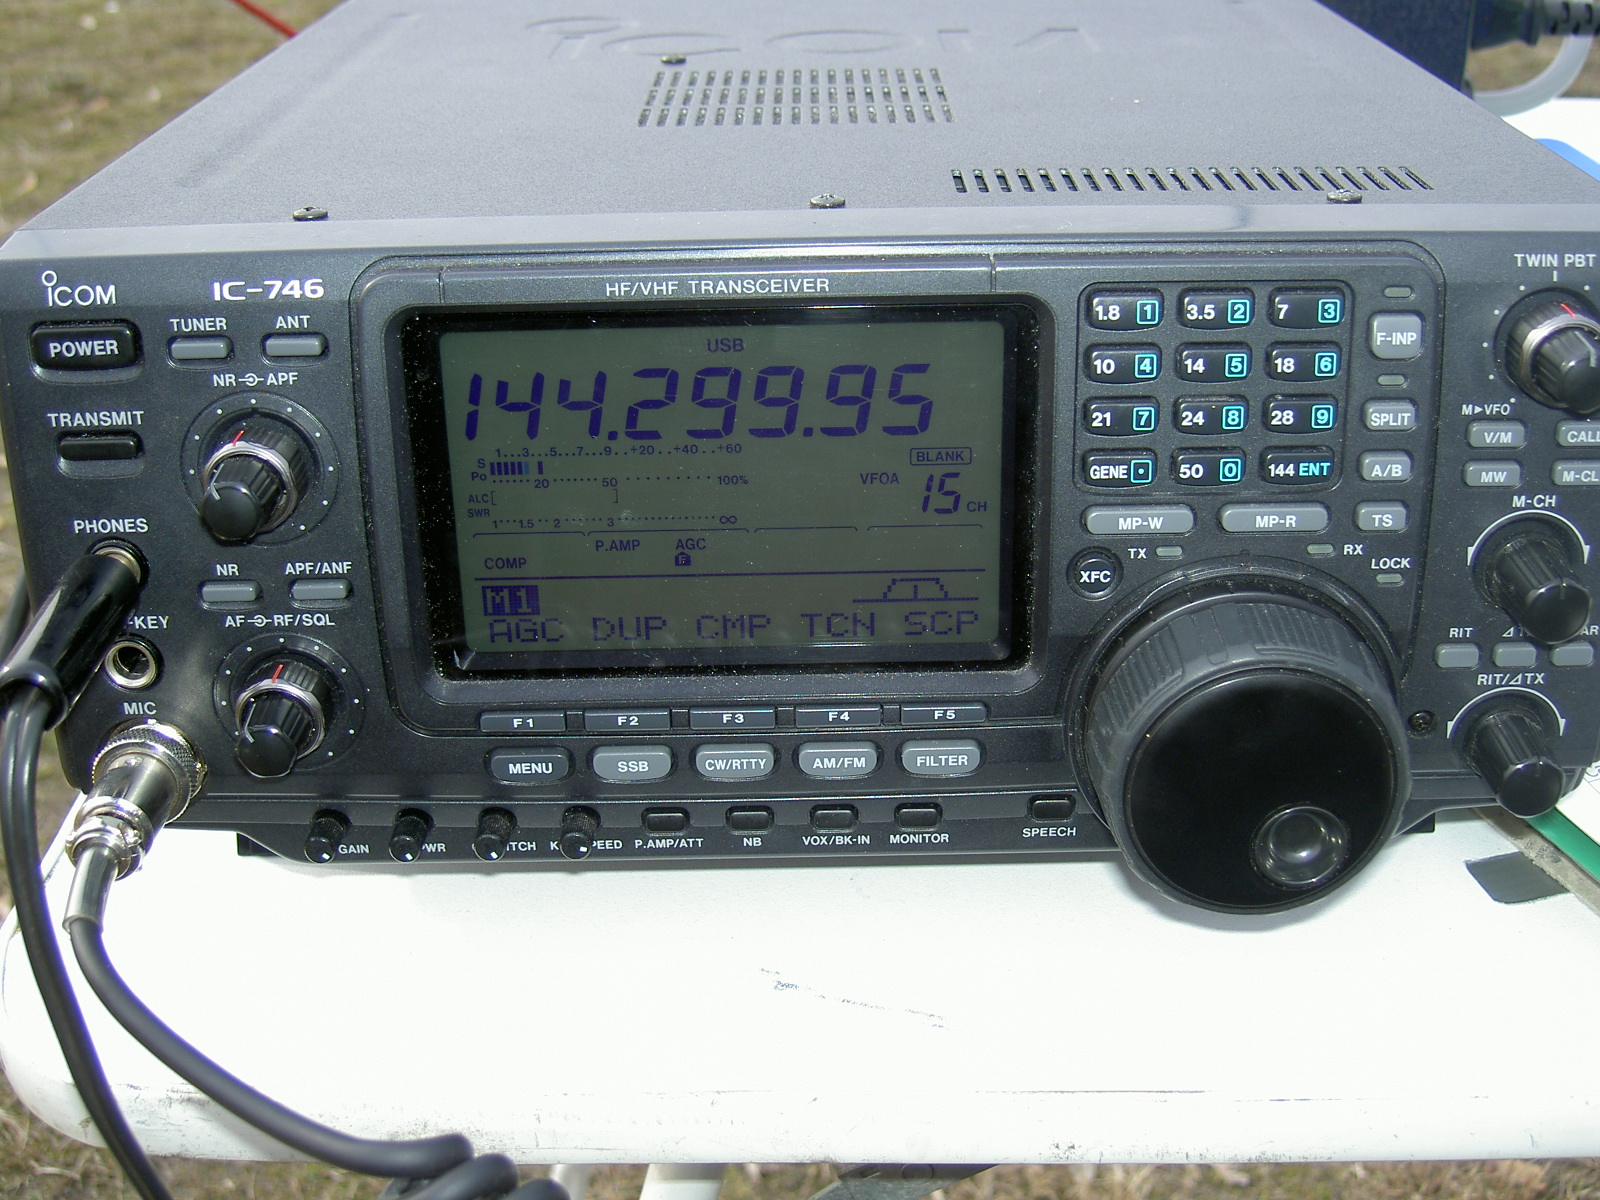
\includegraphics[width=0.85\textwidth]{foto/117}
    \caption{\scriptsize Ein Transceiver (Funkgerät) für den Amateurfunk}
    \label{n_erste_schritte_transceiver}
\end{figure}

    \end{column}
   \begin{column}{0.48\textwidth}
       \begin{itemize}
  \item Jeder darf Funkgeräte kaufen und besitzen
  \item und Amateurfunksendungen empfangen
  \end{itemize}

   \end{column}
\end{columns}

\end{frame}

\begin{frame}
\only<1>{
\begin{QQuestion}{VD102}{Was gilt in Bezug auf den Empfang von Amateurfunkaussendungen?}{Die Anerkennung als \glqq SWL\grqq{} ist erforderlich in Verbindung mit der Mitgliedschaft in einer Amateurfunkvereinigung.}
{Es dürfen nur TKG-zugelassene Empfangsgeräte verwendet werden.}
{Es bedarf der Zuteilung eines Hörerrufzeichens aus der \glqq DE-Reihe\grqq{}.}
{Es ist keine Zulassung zur Teilnahme am Amateurfunkdienst erforderlich.}
\end{QQuestion}

}
\only<2>{
\begin{QQuestion}{VD102}{Was gilt in Bezug auf den Empfang von Amateurfunkaussendungen?}{Die Anerkennung als \glqq SWL\grqq{} ist erforderlich in Verbindung mit der Mitgliedschaft in einer Amateurfunkvereinigung.}
{Es dürfen nur TKG-zugelassene Empfangsgeräte verwendet werden.}
{Es bedarf der Zuteilung eines Hörerrufzeichens aus der \glqq DE-Reihe\grqq{}.}
{\textbf{\textcolor{DARCgreen}{Es ist keine Zulassung zur Teilnahme am Amateurfunkdienst erforderlich.}}}
\end{QQuestion}

}
\end{frame}

\begin{frame}
\frametitle{Ein Funkamateur darf senden}
\begin{columns}
    \begin{column}{0.48\textwidth}
    
\begin{figure}
    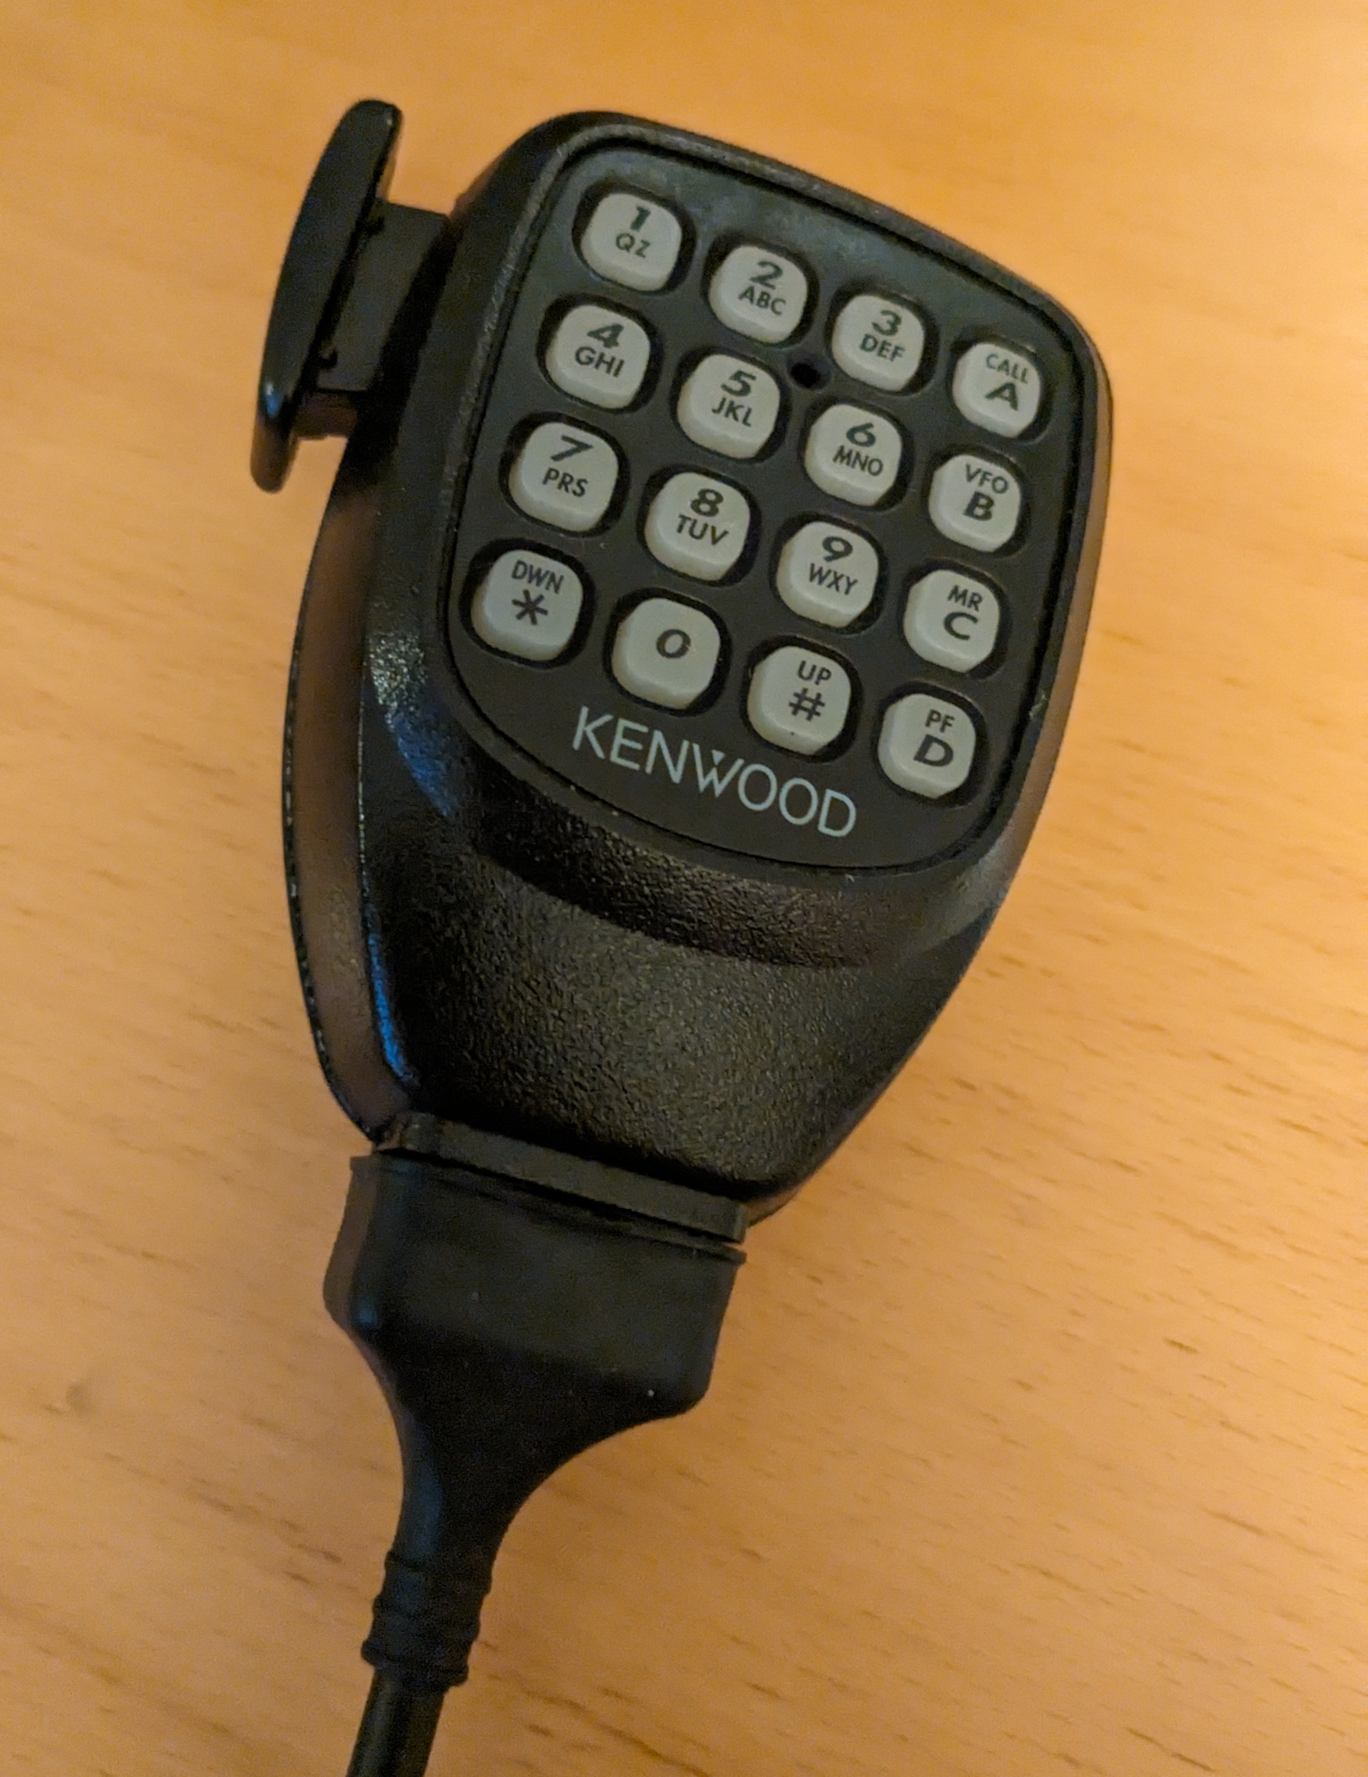
\includegraphics[width=0.85\textwidth]{foto/118}
    \caption{\scriptsize Handmikrofon mit PTT-Taste (links oben)}
    \label{n_erste_schritte_ptt}
\end{figure}

    \end{column}
   \begin{column}{0.48\textwidth}
       Auf Sendung gehen (die PTT-Taste drücken)

\begin{itemize}
  \item Taste am Funkgerät oder Mikrofon
  \item Schaltet den Transceiver von Empfangs- auf Sendebetrieb um
  \end{itemize}

   \end{column}
\end{columns}

\end{frame}

\begin{frame}
\only<1>{
\begin{QQuestion}{NF108}{Wie wird die Taste am Mikrofon bezeichnet, mit der man einen Transceiver auf Sendung schalten kann?}{RIT}
{VOX}
{PTT}
{SSB}
\end{QQuestion}

}
\only<2>{
\begin{QQuestion}{NF108}{Wie wird die Taste am Mikrofon bezeichnet, mit der man einen Transceiver auf Sendung schalten kann?}{RIT}
{VOX}
{\textbf{\textcolor{DARCgreen}{PTT}}}
{SSB}
\end{QQuestion}

}
\end{frame}

\begin{frame}
\frametitle{Mathematische Grundkenntnisse}
\begin{itemize}
  \item Im Amateurfunk werden Grundkenntnisse in Mathematik benötigt
  \item Je nach Klasse mehr Wissen notwendig
  \item Der Lehrgang unterstützt, kann aber nicht alles notwendige Wissen vermitteln
  \end{itemize}
\end{frame}

\begin{frame}
\only<1>{
\begin{QQuestion}{NA101}{Ein \qty{20}{\m} langer Draht wird bei 2/3 seiner Länge zertrennt. Wie lang sind die resultierenden Stücke in etwa?}{\qty{14,44}{\m} und \qty{5,56}{\m}}
{\qty{12,22}{\m} und \qty{7,78}{\m}}
{\qty{11,11}{\m} und \qty{8,89}{\m}}
{\qty{13,33}{\m} und \qty{6,67}{\m}}
\end{QQuestion}

}
\only<2>{
\begin{QQuestion}{NA101}{Ein \qty{20}{\m} langer Draht wird bei 2/3 seiner Länge zertrennt. Wie lang sind die resultierenden Stücke in etwa?}{\qty{14,44}{\m} und \qty{5,56}{\m}}
{\qty{12,22}{\m} und \qty{7,78}{\m}}
{\qty{11,11}{\m} und \qty{8,89}{\m}}
{\textbf{\textcolor{DARCgreen}{\qty{13,33}{\m} und \qty{6,67}{\m}}}}
\end{QQuestion}

}
\end{frame}

\begin{frame}
\only<1>{
\begin{QQuestion}{NA103}{Laut Datenblatt wiegen \qty{100}{\m} eines bestimmten Drahtes 210~g. Ein vorliegendes Drahtstück desselben Materials wiegt 55~g. Wie lang ist das Drahtstück in etwa?}{\qty{38,2}{\m}}
{\qty{382}{\m}}
{\qty{115}{\m}}
{\qty{26,2}{\m}}
\end{QQuestion}

}
\only<2>{
\begin{QQuestion}{NA103}{Laut Datenblatt wiegen \qty{100}{\m} eines bestimmten Drahtes 210~g. Ein vorliegendes Drahtstück desselben Materials wiegt 55~g. Wie lang ist das Drahtstück in etwa?}{\qty{38,2}{\m}}
{\qty{382}{\m}}
{\qty{115}{\m}}
{\textbf{\textcolor{DARCgreen}{\qty{26,2}{\m}}}}
\end{QQuestion}

}
\end{frame}

\begin{frame}
\only<1>{
\begin{QQuestion}{NA102}{Aus \qty{250}{\m} Draht sollen Antennen hergestellt werden. Pro Antenne werden \qty{18,5}{\m} benötigt. Wie viele Antennen können maximal aus dem vorhandenen Draht hergestellt werden?}{13}
{14}
{12}
{15}
\end{QQuestion}

}
\only<2>{
\begin{QQuestion}{NA102}{Aus \qty{250}{\m} Draht sollen Antennen hergestellt werden. Pro Antenne werden \qty{18,5}{\m} benötigt. Wie viele Antennen können maximal aus dem vorhandenen Draht hergestellt werden?}{\textbf{\textcolor{DARCgreen}{13}}}
{14}
{12}
{15}
\end{QQuestion}

}
\end{frame}%ENDCONTENT


\section{Rufzeichen}
\label{section:rufzeichen}
\begin{frame}%STARTCONTENT

\frametitle{Rufzeichen}
\begin{columns}
    \begin{column}{0.48\textwidth}
    
\begin{figure}
    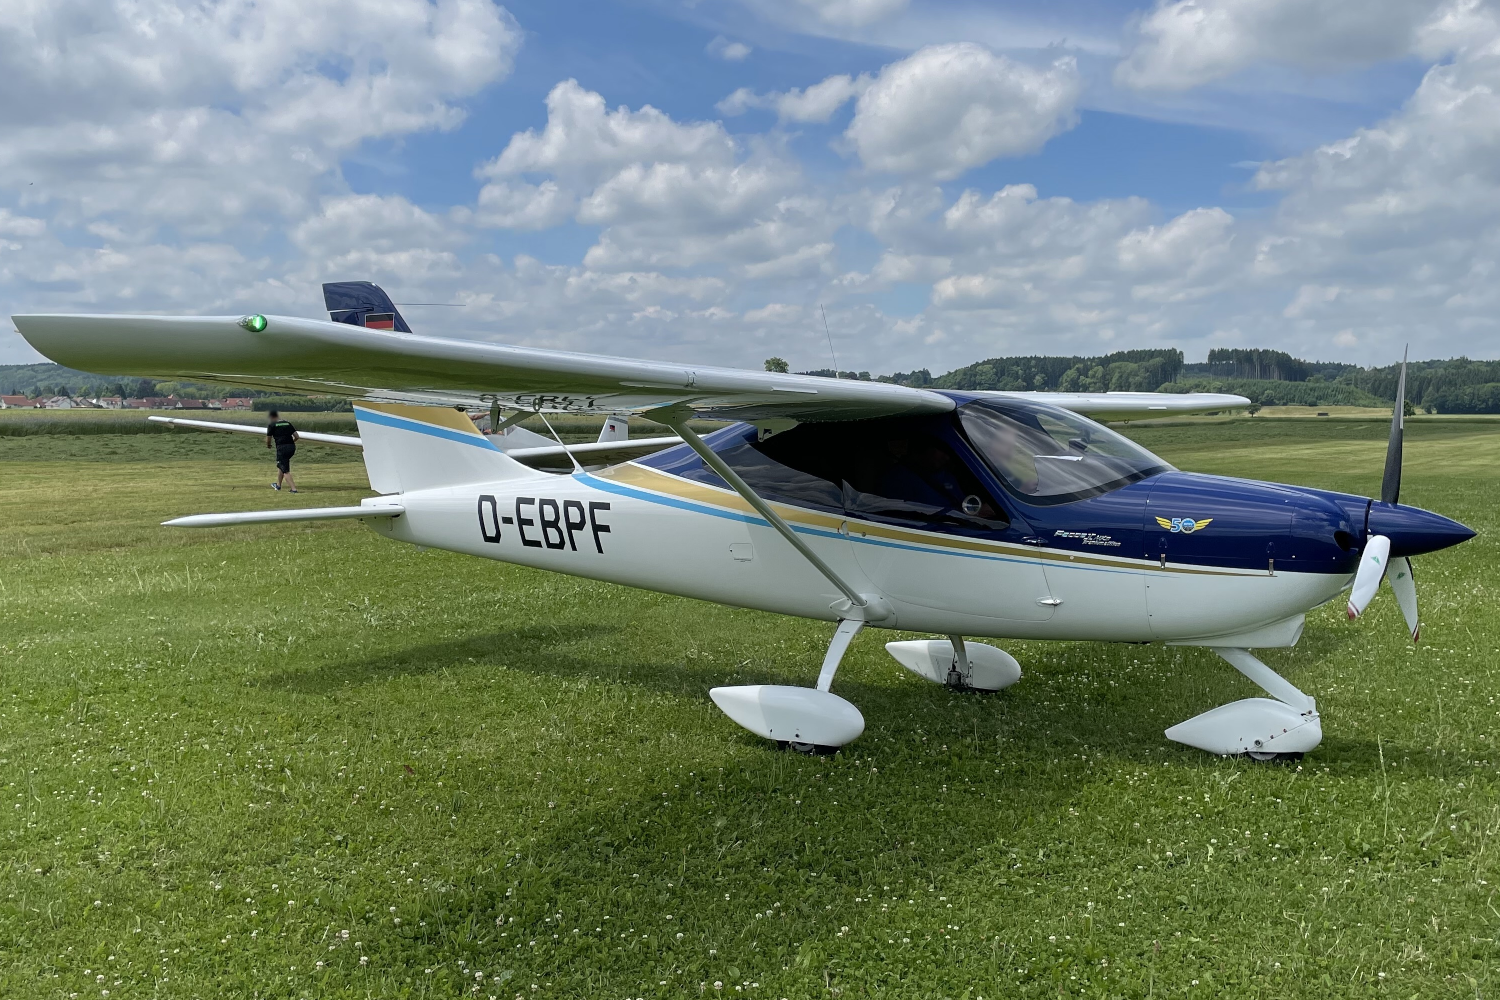
\includegraphics[width=0.85\textwidth]{foto/167}
    \caption{\scriptsize Flugzeug mit dem Rufzeichen DEBPF}
    \label{rufzeichen_flugzeug}
\end{figure}

    \end{column}
   \begin{column}{0.48\textwidth}
       \begin{itemize}
  \item Funkstationen verwenden Rufzeichen, um sich zu identifizieren
  \item Folge von Buchstaben und Ziffern
  \item Jedes mit Funk ausgerüstete Flugzeug und Schiff hat ein Rufzeichen
  \end{itemize}

   \end{column}
\end{columns}

\end{frame}

\begin{frame}
\frametitle{Amateurfunkrufzeichen}
\begin{itemize}
  \item Persönliches Rufzeichen wird zugeteilt
  \item Weltweit eindeutig
  \item Muss am Anfang und Ende jeder Verbindung genannt werden
  \item Und alle 10 Minuten bei längeren Verbindungen
  \end{itemize}
\end{frame}

\begin{frame}
\only<1>{
\begin{QQuestion}{VD207}{Woran erkennt man eine Amateurfunkstelle im Funkbetrieb?}{Am Amateurfunkrufzeichen}
{Am benutzten Frequenzbereich}
{An der verwendeten Sendeart}
{An der Modulation}
\end{QQuestion}

}
\only<2>{
\begin{QQuestion}{VD207}{Woran erkennt man eine Amateurfunkstelle im Funkbetrieb?}{\textbf{\textcolor{DARCgreen}{Am Amateurfunkrufzeichen}}}
{Am benutzten Frequenzbereich}
{An der verwendeten Sendeart}
{An der Modulation}
\end{QQuestion}

}
\end{frame}

\begin{frame}
\only<1>{
\begin{QQuestion}{VD205}{Wann muss der Funkamateur sein Rufzeichen nennen?}{Mindestens alle 15~Minuten während einer Funkverbindung}
{Auf Verlangen einer anderen am Funkverkehr beteiligten Funkstelle}
{Am Anfang und am Ende jeder Funkverbindung sowie mindestens alle 10~Minuten}
{Spätestens 5~Minuten nach einer ununterbrochenen Aussendung}
\end{QQuestion}

}
\only<2>{
\begin{QQuestion}{VD205}{Wann muss der Funkamateur sein Rufzeichen nennen?}{Mindestens alle 15~Minuten während einer Funkverbindung}
{Auf Verlangen einer anderen am Funkverkehr beteiligten Funkstelle}
{\textbf{\textcolor{DARCgreen}{Am Anfang und am Ende jeder Funkverbindung sowie mindestens alle 10~Minuten}}}
{Spätestens 5~Minuten nach einer ununterbrochenen Aussendung}
\end{QQuestion}

}
\end{frame}%ENDCONTENT


\section{Internationale Buchstabiertafel}
\label{section:buchstabiertafel}
\begin{frame}%STARTCONTENT
\begin{itemize}
  \item Manche Buchstaben lassen sich schwer voneinander unterscheiden
  \item Noch schwieriger bei leisem oder schlechtem Empfang
  \end{itemize}

\end{frame}

\begin{frame}
\frametitle{Lösung}
\begin{itemize}
  \item Jedem Buchstaben wird ein Wort zugeordnet
  \item Anstatt des Buchstabens wird das Wort ausgesprochen
  \end{itemize}
\end{frame}

\begin{frame}
\frametitle{Buchstabiertafeln}
\begin{itemize}
  \item In Deutschland ist die deutsche Buchstabiertafel bekannt
  \item Im Amateurfunk wird die internationale Buchstabiertafel verwendet
  \item Erste Einführung 1927 durch die International Telecommunication Union (ITU)
  \item Anhang 14 der Radio Regulations (RR)
  \item Wird auch in der Luftfahrt, dem Seefunk und von der NATO verwendet
  \end{itemize}

\end{frame}

\begin{frame}
\begin{columns}
    \begin{column}{0.48\textwidth}
    \begin{table}
\begin{DARCtabular}{cll}
     Buchstabe  & Wort  & Aussprache   \\
     A  & Alfa  & AL-FA   \\
     B  & Bravo  & BRA-WO   \\
     C  & Charlie  & TSCHA-LI   \\
     D  & Delta  & DELL-TA   \\
     E  & Echo  & ECK-KO   \\
     F  & Foxtrot  & FOX-TROTT   \\
     G  & Golf  & GOLF   \\
     H  & Hotel  & HO-TELL   \\
     I  & India  & IN-DI-AH   \\
     J  & Juliett  & DJU-LI-ETT   \\
     K  & Kilo  & KI-LO   \\
     L  & Lima  & LI-MA   \\
     M  & Mike  & MAIK   \\
\end{DARCtabular}
\caption{Die ITU-Buchstabiertafel}
\label{n_buchstabiertafel_1}
\end{table}

    \end{column}
   \begin{column}{0.48\textwidth}
       \begin{table}
\begin{DARCtabular}{cll}
     Buchstabe  & Wort  & Aussprache   \\
     N  & November  & NO-WEM-BER   \\
     O  & Oscar  & OSS-KAR   \\
     P  & Papa  & PA-PA   \\
     Q  & Quebec  & KWE-BECK   \\
     R  & Romeo  & RO-MI-O   \\
     S  & Sierra  & SIER-RA   \\
     T  & Tango  & TÄNG-GO   \\
     U  & Uniform  & JU-NI-FORM   \\
     V  & Victor  & WICK-TOR   \\
     W  & Whiskey  & WISS-KI   \\
     X  & X-ray  & ÄX-RÄI   \\
     Y  & Yankee  & JENG-KI   \\
     Z  & Zulu  & SUH-LUH   \\
\end{DARCtabular}
\caption{Die ITU-Buchstabiertafel}
\label{n_buchstabiertafel_2}
\end{table}

   \end{column}
\end{columns}

\end{frame}

\begin{frame}
\only<1>{
\begin{QQuestion}{VD206}{Welches Buchstabieralphabet ist nach der Verfügung 13/2005 bei der Nennung des Rufzeichens zur Identifikation einer Amateurfunkstation zu verwenden?}{Das englische Buchstabieralphabet der ITU-Konferenz in Madrid von 1932}
{Das europäische Buchstabieralphabet von 1992}
{Das internationale Buchstabieralphabet nach den Radio Regulations (Anhang 14)}
{Das deutsche Buchstabieralphabet nach DIN 5009}
\end{QQuestion}

}
\only<2>{
\begin{QQuestion}{VD206}{Welches Buchstabieralphabet ist nach der Verfügung 13/2005 bei der Nennung des Rufzeichens zur Identifikation einer Amateurfunkstation zu verwenden?}{Das englische Buchstabieralphabet der ITU-Konferenz in Madrid von 1932}
{Das europäische Buchstabieralphabet von 1992}
{\textbf{\textcolor{DARCgreen}{Das internationale Buchstabieralphabet nach den Radio Regulations (Anhang 14)}}}
{Das deutsche Buchstabieralphabet nach DIN 5009}
\end{QQuestion}

}
\end{frame}

\begin{frame}
\only<1>{
\begin{QQuestion}{BA103}{Wie wird das Rufzeichen \glqq DK5WP\grqq{} mit dem internationalen Buchstabieralphabet  buchstabiert?}{Delta Kilowatt 5 Whiskey Paris}
{Delta Kilo 5 William Paris}
{Delta Kilo 5 Whiskey Papa}
{Delta Kilowatt 5 William Papa}
\end{QQuestion}

}
\only<2>{
\begin{QQuestion}{BA103}{Wie wird das Rufzeichen \glqq DK5WP\grqq{} mit dem internationalen Buchstabieralphabet  buchstabiert?}{Delta Kilowatt 5 Whiskey Paris}
{Delta Kilo 5 William Paris}
{\textbf{\textcolor{DARCgreen}{Delta Kilo 5 Whiskey Papa}}}
{Delta Kilowatt 5 William Papa}
\end{QQuestion}

}
\end{frame}

\begin{frame}
\only<1>{
\begin{QQuestion}{BA104}{Wie wird das Rufzeichen \glqq DL1FLO\grqq{} mit dem internationalen Buchstabieralphabet  buchstabiert?}{Delta Lima 1 Florida Lima Oslo}
{Delta London 1 Foxtrot London Oslo}
{Delta Lima 1 Foxtrot Lima Oscar}
{Delta London 1 Florida London Oscar}
\end{QQuestion}

}
\only<2>{
\begin{QQuestion}{BA104}{Wie wird das Rufzeichen \glqq DL1FLO\grqq{} mit dem internationalen Buchstabieralphabet  buchstabiert?}{Delta Lima 1 Florida Lima Oslo}
{Delta London 1 Foxtrot London Oslo}
{\textbf{\textcolor{DARCgreen}{Delta Lima 1 Foxtrot Lima Oscar}}}
{Delta London 1 Florida London Oscar}
\end{QQuestion}

}
\end{frame}

\begin{frame}
\only<1>{
\begin{QQuestion}{BA110}{Wie wird das Rufzeichen \glqq IG9/DL4HR\grqq{} mit dem internationalen Buchstabieralphabet  buchstabiert?}{Italy Golf 9 Stroke Delta Lima 4 Honolulu Romeo}
{India Guatemala 9 Stroke Delta Lima 4 Honolulu Romeo}
{India Golf 9 Stroke Delta Lima 4 Hotel Romeo}
{Italy Guatemala 9 Stroke Delta Lima 4 Hotel Romeo}
\end{QQuestion}

}
\only<2>{
\begin{QQuestion}{BA110}{Wie wird das Rufzeichen \glqq IG9/DL4HR\grqq{} mit dem internationalen Buchstabieralphabet  buchstabiert?}{Italy Golf 9 Stroke Delta Lima 4 Honolulu Romeo}
{India Guatemala 9 Stroke Delta Lima 4 Honolulu Romeo}
{\textbf{\textcolor{DARCgreen}{India Golf 9 Stroke Delta Lima 4 Hotel Romeo}}}
{Italy Guatemala 9 Stroke Delta Lima 4 Hotel Romeo}
\end{QQuestion}

}
\end{frame}

\begin{frame}
\only<1>{
\begin{QQuestion}{BA109}{Wie wird das Rufzeichen \glqq DO9XJZ\grqq{} mit dem internationalen Buchstabieralphabet  buchstabiert?}{Delta Oscar 9 Xavier Juliett Zebra}
{Delta Oscar 9 X-ray Japan Zebra}
{Delta Oscar 9 X-ray Juliett Zulu}
{Delta Oscar 9 Xavier Japan Zulu}
\end{QQuestion}

}
\only<2>{
\begin{QQuestion}{BA109}{Wie wird das Rufzeichen \glqq DO9XJZ\grqq{} mit dem internationalen Buchstabieralphabet  buchstabiert?}{Delta Oscar 9 Xavier Juliett Zebra}
{Delta Oscar 9 X-ray Japan Zebra}
{\textbf{\textcolor{DARCgreen}{Delta Oscar 9 X-ray Juliett Zulu}}}
{Delta Oscar 9 Xavier Japan Zulu}
\end{QQuestion}

}
\end{frame}

\begin{frame}
\only<1>{
\begin{QQuestion}{BA101}{Wie wird das Rufzeichen \glqq DD4UQ\grqq{} mit dem internationalen Buchstabieralphabet  buchstabiert?}{Delta Delta 4 Uruguay Queen}
{Delta Delta 4 Uniform Quebec}
{Denmark Denmark 4 Uniform Queen}
{Denmark Denmark 4 Uruguay Quebec}
\end{QQuestion}

}
\only<2>{
\begin{QQuestion}{BA101}{Wie wird das Rufzeichen \glqq DD4UQ\grqq{} mit dem internationalen Buchstabieralphabet  buchstabiert?}{Delta Delta 4 Uruguay Queen}
{\textbf{\textcolor{DARCgreen}{Delta Delta 4 Uniform Quebec}}}
{Denmark Denmark 4 Uniform Queen}
{Denmark Denmark 4 Uruguay Quebec}
\end{QQuestion}

}
\end{frame}

\begin{frame}
\only<1>{
\begin{QQuestion}{BA105}{Wie wird das Rufzeichen \glqq DL4YBZ\grqq{} mit dem internationalen Buchstabieralphabet  buchstabiert?}{Delta Lima 4 Ypsilon Baker Zulu}
{Delta Lima 4 Yankee Baker Zebra}
{Delta Lima 4 Ypsilon Bravo Zebra}
{Delta Lima 4 Yankee Bravo Zulu}
\end{QQuestion}

}
\only<2>{
\begin{QQuestion}{BA105}{Wie wird das Rufzeichen \glqq DL4YBZ\grqq{} mit dem internationalen Buchstabieralphabet  buchstabiert?}{Delta Lima 4 Ypsilon Baker Zulu}
{Delta Lima 4 Yankee Baker Zebra}
{Delta Lima 4 Ypsilon Bravo Zebra}
{\textbf{\textcolor{DARCgreen}{Delta Lima 4 Yankee Bravo Zulu}}}
\end{QQuestion}

}
\end{frame}

\begin{frame}
\only<1>{
\begin{QQuestion}{BA106}{Wie wird das Rufzeichen \glqq DM4EAX\grqq{} mit dem internationalen Buchstabieralphabet  buchstabiert?}{Delta Madagascar 4 Echo Amerika X-ray}
{Delta Mike 4 Ecuador Amerika X-ray}
{Delta Mike 4 Echo Alfa X-ray}
{Delta Madagascar 4 Ecuador Alfa X-ray}
\end{QQuestion}

}
\only<2>{
\begin{QQuestion}{BA106}{Wie wird das Rufzeichen \glqq DM4EAX\grqq{} mit dem internationalen Buchstabieralphabet  buchstabiert?}{Delta Madagascar 4 Echo Amerika X-ray}
{Delta Mike 4 Ecuador Amerika X-ray}
{\textbf{\textcolor{DARCgreen}{Delta Mike 4 Echo Alfa X-ray}}}
{Delta Madagascar 4 Ecuador Alfa X-ray}
\end{QQuestion}

}
\end{frame}

\begin{frame}
\only<1>{
\begin{QQuestion}{BA102}{Wie wird das Rufzeichen \glqq DK1KC\grqq{} mit dem internationalen Buchstabieralphabet  buchstabiert?}{Delta Kilowatt 1 Kilowatt Caesar}
{Delta Kilo 1 Kilo Charlie}
{Denmark Kilo 1 Kilo Caesar}
{Denmark Kilowatt 1 Kilowatt Charlie}
\end{QQuestion}

}
\only<2>{
\begin{QQuestion}{BA102}{Wie wird das Rufzeichen \glqq DK1KC\grqq{} mit dem internationalen Buchstabieralphabet  buchstabiert?}{Delta Kilowatt 1 Kilowatt Caesar}
{\textbf{\textcolor{DARCgreen}{Delta Kilo 1 Kilo Charlie}}}
{Denmark Kilo 1 Kilo Caesar}
{Denmark Kilowatt 1 Kilowatt Charlie}
\end{QQuestion}

}
\end{frame}

\begin{frame}
\only<1>{
\begin{QQuestion}{BA107}{Wie wird das Rufzeichen \glqq DN9RO/p\grqq{} mit dem internationalen Buchstabieralphabet  buchstabiert?}{Delta November 9 Radio Oslo Stroke portable}
{Delta November 9 Romeo Oscar Stroke portable}
{Delta Nordpol 9 Radio Oslo Stroke portable}
{Delta Nordpol 9 Romeo Oscar Stroke portable}
\end{QQuestion}

}
\only<2>{
\begin{QQuestion}{BA107}{Wie wird das Rufzeichen \glqq DN9RO/p\grqq{} mit dem internationalen Buchstabieralphabet  buchstabiert?}{Delta November 9 Radio Oslo Stroke portable}
{\textbf{\textcolor{DARCgreen}{Delta November 9 Romeo Oscar Stroke portable}}}
{Delta Nordpol 9 Radio Oslo Stroke portable}
{Delta Nordpol 9 Romeo Oscar Stroke portable}
\end{QQuestion}

}
\end{frame}

\begin{frame}
\only<1>{
\begin{QQuestion}{BA108}{Wie wird das Rufzeichen \glqq DN9STV\grqq{} mit dem internationalen Buchstabieralphabet  buchstabiert?}{Delta November 9 Santiago Texas Victor}
{Delta November 9 Sierra Texas Vulcano}
{Delta November 9 Santiago Tango Vulcano}
{Delta November 9 Sierra Tango Victor}
\end{QQuestion}

}
\only<2>{
\begin{QQuestion}{BA108}{Wie wird das Rufzeichen \glqq DN9STV\grqq{} mit dem internationalen Buchstabieralphabet  buchstabiert?}{Delta November 9 Santiago Texas Victor}
{Delta November 9 Sierra Texas Vulcano}
{Delta November 9 Santiago Tango Vulcano}
{\textbf{\textcolor{DARCgreen}{Delta November 9 Sierra Tango Victor}}}
\end{QQuestion}

}
\end{frame}%ENDCONTENT


\section{Betriebsabwicklung}
\label{section:betriebsabwicklung}
\begin{frame}%STARTCONTENT

\frametitle{Ablauf im Amateurfunk}
\begin{itemize}
  \item Es gibt keine verpflichtenden Vorgaben außer Nennung des Rufzeichens
  \item Es macht aber Sinn, sich an der Betriebsabwicklung zu orientieren
  \end{itemize}

\end{frame}

\begin{frame}
\frametitle{Freie Frequenz finden}
\begin{itemize}
  \item Frequenzen werden gemeinsam genutzt
  \item Erst hören, ob die Frequenz frei ist
  \item Zwei- bis dreimal kurz nachfragen, ob die Frequenz frei ist
  \end{itemize}

\end{frame}

\begin{frame}
\frametitle{Anruf starten}
    \pause
    
\frametitle{Allgemeiner Anruf}
\begin{itemize}
  \item Geht an \emph{alle} Stationen
  \item Beginnt mit der internationalen Abkürzung \emph{CQ}
  \end{itemize}
    \pause
    
\frametitle{Gezielter Anruf}
\begin{itemize}
  \item Antwort von einer bestimmten Station erwartet
  \end{itemize}
    \pause
    In der Antwort wird erst das Rufzeichen der anrufenden Station, dann das eigene genannt

\end{frame}

\begin{frame}
\frametitle{Allgemeiner Anruf}
    \pause\QSOown{Ist diese Frequenz frei? DL1PZ}\pause\QSOother{\emph{(keine Antwort)}}\pause\QSOown{Ist diese Frequenz frei? DL1PZ}\pause\QSOother{\emph{(keine Antwort)}}\pause\QSOown{CQ CQ hier ist DL1PZ mit einem allgemeinen Anruf, hier ist DL1PZ und hört.}\pause\QSOother{DL1PZ hier ist DL9MJ bitte kommen}


\end{frame}

\begin{frame}
\frametitle{Gezielter Anruf}
    \pause\QSOown{DL9MJ für DL1PZ bitte kommen}\pause\QSOother{DL1PZ hier ist DL9MJ}


\end{frame}

\begin{frame}
\only<1>{
\begin{QQuestion}{BB102}{Was bedeutet die betriebliche Abkürzung \glqq CQ\grqq{} im Amateurfunk?}{Allgemeiner Anruf}
{Telegrafie}
{Große Entfernung}
{Contest Query}
\end{QQuestion}

}
\only<2>{
\begin{QQuestion}{BB102}{Was bedeutet die betriebliche Abkürzung \glqq CQ\grqq{} im Amateurfunk?}{\textbf{\textcolor{DARCgreen}{Allgemeiner Anruf}}}
{Telegrafie}
{Große Entfernung}
{Contest Query}
\end{QQuestion}

}
\end{frame}

\begin{frame}
\only<1>{
\begin{QQuestion}{BE105}{Sie möchten einen Allgemeinen Anruf in Telefonie im \qty{10}{\m}-Band beginnen. Sie finden eine Frequenz, auf der Sie keine Signale hören. Wie gehen Sie vor?}{Ich frage zwei- bis dreimal, ob die Frequenz besetzt ist. Erfolgt keine Antwort, rufe ich CQ.}
{Ich beobachte die Frequenz für einige Sekunden. Wenn ich weiterhin keine Signale höre, rufe ich CQ.}
{Da ich auf der Frequenz kein Signal höre, kann ich mit meinem CQ-Ruf beginnen.}
{Ich stimme meinen Sender auf der Frequenz ab und starte dann meinen CQ-Ruf.}
\end{QQuestion}

}
\only<2>{
\begin{QQuestion}{BE105}{Sie möchten einen Allgemeinen Anruf in Telefonie im \qty{10}{\m}-Band beginnen. Sie finden eine Frequenz, auf der Sie keine Signale hören. Wie gehen Sie vor?}{\textbf{\textcolor{DARCgreen}{Ich frage zwei- bis dreimal, ob die Frequenz besetzt ist. Erfolgt keine Antwort, rufe ich CQ.}}}
{Ich beobachte die Frequenz für einige Sekunden. Wenn ich weiterhin keine Signale höre, rufe ich CQ.}
{Da ich auf der Frequenz kein Signal höre, kann ich mit meinem CQ-Ruf beginnen.}
{Ich stimme meinen Sender auf der Frequenz ab und starte dann meinen CQ-Ruf.}
\end{QQuestion}

}
\end{frame}

\begin{frame}
\only<1>{
\begin{QQuestion}{BE101}{Wie können Sie eine Amateurfunkverbindung zum Beispiel beginnen?}{Durch Benutzen der internationalen Betriebsabkürzung CQ bzw. mit einem allgemeinen Anruf; mit einem gezielten Anruf an eine bestimmte Station oder mit einer Antwort auf einen allgemeinen Anruf, jeweils mit Nennung des eigenen Rufzeichens.}
{Durch wiederholtes Aussenden der internationalen Q-Gruppe \glqq QRZ?\grqq{} mit angehängtem eigenen Rufzeichen und dem Abhören der Frequenz in den Sendepausen.}
{Durch mehrmaliges, bei schlechten Ausbreitungsbedingungen häufiges Aussenden der Abkürzung CQ, des eigenen Rufzeichens und der Q-Gruppe \glqq QTH\grqq{} mit Zwischenhören.}
{Durch das Aussenden Ihres Rufzeichens und des in der IARU festgelegten Auftasttones von \qty{1750}{\Hz}, durch den die abhörenden Stationen Ihren Verbindungswunsch erkennen.}
\end{QQuestion}

}
\only<2>{
\begin{QQuestion}{BE101}{Wie können Sie eine Amateurfunkverbindung zum Beispiel beginnen?}{\textbf{\textcolor{DARCgreen}{Durch Benutzen der internationalen Betriebsabkürzung CQ bzw. mit einem allgemeinen Anruf; mit einem gezielten Anruf an eine bestimmte Station oder mit einer Antwort auf einen allgemeinen Anruf, jeweils mit Nennung des eigenen Rufzeichens.}}}
{Durch wiederholtes Aussenden der internationalen Q-Gruppe \glqq QRZ?\grqq{} mit angehängtem eigenen Rufzeichen und dem Abhören der Frequenz in den Sendepausen.}
{Durch mehrmaliges, bei schlechten Ausbreitungsbedingungen häufiges Aussenden der Abkürzung CQ, des eigenen Rufzeichens und der Q-Gruppe \glqq QTH\grqq{} mit Zwischenhören.}
{Durch das Aussenden Ihres Rufzeichens und des in der IARU festgelegten Auftasttones von \qty{1750}{\Hz}, durch den die abhörenden Stationen Ihren Verbindungswunsch erkennen.}
\end{QQuestion}

}
\end{frame}

\begin{frame}
\only<1>{
\begin{QQuestion}{BE102}{Wie sollten Sie antworten, wenn jemand in Telefonie CQ ruft?}{Ich rufe ebenfalls CQ und nenne das Rufzeichen der rufenden Station mindestens dreimal, anschließend sage ich mindestens fünfmal: \glqq Hier ist (eigenes Rufzeichen buchstabieren)\grqq{}.}
{Ich nenne das Rufzeichen der rufenden Station mindestens fünfmal, und anschließend sage ich mindestens einmal: \glqq Hier ist (eigenes Rufzeichen buchstabieren)\grqq{}.}
{Ich nenne das Rufzeichen der rufenden Station einmal, anschließend sage ich einmal: \glqq Hier ist (eigenes Rufzeichen buchstabieren), bitte kommen\grqq{}.}
{Ich nenne mein Rufzeichen und fordere die rufende Station auf, auf einer anderen Frequenz weiter zu rufen (mindestens zweimal).}
\end{QQuestion}

}
\only<2>{
\begin{QQuestion}{BE102}{Wie sollten Sie antworten, wenn jemand in Telefonie CQ ruft?}{Ich rufe ebenfalls CQ und nenne das Rufzeichen der rufenden Station mindestens dreimal, anschließend sage ich mindestens fünfmal: \glqq Hier ist (eigenes Rufzeichen buchstabieren)\grqq{}.}
{Ich nenne das Rufzeichen der rufenden Station mindestens fünfmal, und anschließend sage ich mindestens einmal: \glqq Hier ist (eigenes Rufzeichen buchstabieren)\grqq{}.}
{\textbf{\textcolor{DARCgreen}{Ich nenne das Rufzeichen der rufenden Station einmal, anschließend sage ich einmal: \glqq Hier ist (eigenes Rufzeichen buchstabieren), bitte kommen\grqq{}.}}}
{Ich nenne mein Rufzeichen und fordere die rufende Station auf, auf einer anderen Frequenz weiter zu rufen (mindestens zweimal).}
\end{QQuestion}

}
\end{frame}

\begin{frame}
\frametitle{Unklare Verständigung}
    \pause\QSOown{D\emph{(krschkrsch)}MJ für DK5WP, bitte kommen}\pause\QSOother{Hier ist DL9MJ, wurde ich gerufen?}
    \pause
    Nachfragen, ob man gemeint war



\end{frame}

\begin{frame}
\only<1>{
\begin{QQuestion}{BE103}{Ihr Rufzeichen ist DH7RW. Sie hören unvollständig \glqq ...~7 Romeo Whiskey\grqq{}. Wie reagieren Sie?}{Ich antworte: \glqq Bitte QSY!\grqq{}.}
{Ich antworte: \glqq Bitte QSL!\grqq{}    }
{Ich antworte: \glqq Hier ist DH7RW, wurde ich gerufen?\grqq{}}
{Ich freue mich auf eine Antwort aus 7R - Algerien.}
\end{QQuestion}

}
\only<2>{
\begin{QQuestion}{BE103}{Ihr Rufzeichen ist DH7RW. Sie hören unvollständig \glqq ...~7 Romeo Whiskey\grqq{}. Wie reagieren Sie?}{Ich antworte: \glqq Bitte QSY!\grqq{}.}
{Ich antworte: \glqq Bitte QSL!\grqq{}    }
{\textbf{\textcolor{DARCgreen}{Ich antworte: \glqq Hier ist DH7RW, wurde ich gerufen?\grqq{}}}}
{Ich freue mich auf eine Antwort aus 7R - Algerien.}
\end{QQuestion}

}
\end{frame}

\begin{frame}
\frametitle{Anruf beenden}
\begin{itemize}
  \item Die Frequenz wird der anrufenden Station überlassen
  \item Falls die antwortende Station zwischendurch von einer weiteren Station gerufen wurde, soll sie sich mit dieser auf eine andere Frequenz einigen, um der bisherigen Station die Frequenz zurückzugeben
  \end{itemize}
\end{frame}

\begin{frame}
\only<1>{
\begin{QQuestion}{BE108}{Sie haben eine Funkverbindung mit einer vorher \glqq CQ\grqq{} rufenden Station beendet. Anschließend werden Sie von einer anderen Station gerufen. Wie verhalten Sie sich?}{Ich bleibe auf der Frequenz und tätige ein QSO mit der neu rufenden Station.}
{Ich verständige mich mit der neuen Gegenstation auf eine andere Frequenz und führe dort das QSO weiter.}
{Ich gehe etwa \qty{1}{\kHz} neben die bisherige Frequenz und rufe dort die anrufende Station.}
{Ich reagiere nicht auf den Anruf, weil die Frequenz der Station gehört, die CQ gerufen hat.}
\end{QQuestion}

}
\only<2>{
\begin{QQuestion}{BE108}{Sie haben eine Funkverbindung mit einer vorher \glqq CQ\grqq{} rufenden Station beendet. Anschließend werden Sie von einer anderen Station gerufen. Wie verhalten Sie sich?}{Ich bleibe auf der Frequenz und tätige ein QSO mit der neu rufenden Station.}
{\textbf{\textcolor{DARCgreen}{Ich verständige mich mit der neuen Gegenstation auf eine andere Frequenz und führe dort das QSO weiter.}}}
{Ich gehe etwa \qty{1}{\kHz} neben die bisherige Frequenz und rufe dort die anrufende Station.}
{Ich reagiere nicht auf den Anruf, weil die Frequenz der Station gehört, die CQ gerufen hat.}
\end{QQuestion}

}
\end{frame}%ENDCONTENT


\section{Das RST-System}
\label{section:rst}
\begin{frame}%STARTCONTENT

\frametitle{Das RST-System}
Qualität der Funkverbindung hängt ab von

\begin{itemize}
  \item Sendeleistung
  \item verwendete Antenne
  \item Entfernung
  \item aktuelle Ausbreitungsbedingungen
  \end{itemize}
    \pause
    Im Rapport beschreibt die empfangende Station die Qualität der Verbindung

\end{frame}

\begin{frame}
\only<1>{
\begin{QQuestion}{BE201}{Was versteht man unter dem RST-Rapport? Es ist eine Kurzformel,~...}{um die Sendeleistung zu beschreiben.}
{um die Empfangsqualität zu beschreiben.}
{um den Ionosphärenzustand zu beschreiben.}
{um die Sonnenfleckenaktivität zu beschreiben.}
\end{QQuestion}

}
\only<2>{
\begin{QQuestion}{BE201}{Was versteht man unter dem RST-Rapport? Es ist eine Kurzformel,~...}{um die Sendeleistung zu beschreiben.}
{\textbf{\textcolor{DARCgreen}{um die Empfangsqualität zu beschreiben.}}}
{um den Ionosphärenzustand zu beschreiben.}
{um die Sonnenfleckenaktivität zu beschreiben.}
\end{QQuestion}

}
\end{frame}

\begin{frame}
\frametitle{RST-System}
\begin{table}
\begin{DARCtabular}{llll}
     Wert  & Bereich  & Bedeutung  & Englisch   \\
     R  & 1 -- 5  & Lesbarkeit  & Readability   \\
     S  & 1 -- 9  & Signalstärke  & Signal Strength   \\
     T  & 1 -- 9  & Tonqualität  & Tone   \\
\end{DARCtabular}
\caption{Die Bestandteile des RST-Rapports}
\label{n_rst}
\end{table}

\end{frame}

\begin{frame}
\frametitle{Readability}
Subjektive Bewertung des Lesbarkeit (Verständlichkeit)

\begin{table}
\begin{DARCtabular}{ll}
     R  & Beurteilung   \\
     1  & nicht lesbar   \\
     2  & zeitweise lesbar   \\
     3 & mit Schwierigkeiten lesbar   \\
     4  & ohne Schwierigkeiten lesbar   \\
     5  & einwandfrei lesbar   \\
\end{DARCtabular}
\caption{Anhaltspunkte für die subjektive Bewertung der Lesbarkeit (Verständlichkeit)}
\label{n_rst_r}
\end{table}
\end{frame}

\begin{frame}
\frametitle{Signal Strength}
Vom Funkgerät ablesen


\begin{figure}
    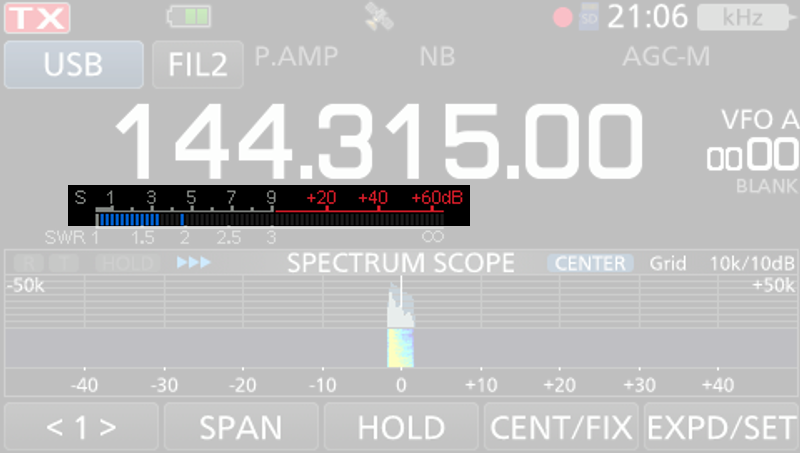
\includegraphics[width=0.85\textwidth]{foto/123}
    \caption{\scriptsize Display eines IC9700-Transceivers, hervorgehoben ist das S-Meter, das den aktuellen Empfangspegel anzeigt}
    \label{n_rst_s-meter}
\end{figure}

\end{frame}

\begin{frame}
\frametitle{Beispiele für RST-Rapporte}
im Sprechfunk

\begin{table}
\begin{DARCtabular}{llcl}
     Verständlichkeit  & S-Meter  &$\rightarrow$ & RST-Rapport   \\
     einwandfrei (=5)  & +\qty{20}{\dB}  &$\rightarrow$ & 59+20dB   \\
     einwandfrei (=5)  & 9  &$\rightarrow$ & 59   \\
     ohne Schwierigkeiten (=4)  & 5  &$\rightarrow$ & 45   \\
     mit Schwierigkeiten (=3)  & 3  &$\rightarrow$ & 33   \\
     unverständlich (=1)  & 3  &$\rightarrow$ & 13   \\
\end{DARCtabular}
\caption{Beispiele für RST-Rapporte im Sprechfunk}
\label{n_rst_beispiele}
\end{table}
\end{frame}

\begin{frame}
\only<1>{
\begin{QQuestion}{BE202}{Was bedeuten die Buchstaben RST, mit denen Sie die Empfangsqualität einer Sendung beurteilen können?}{R = Rufzeichen, S = Standort, T = Tonqualität}
{R = Rufzeichen, S = Signalstärke, T = Tonqualität}
{R = Lesbarkeit, S = Signalstärke, T = Trägerfrequenz}
{R = Lesbarkeit, S = Signalstärke, T = Tonqualität}
\end{QQuestion}

}
\only<2>{
\begin{QQuestion}{BE202}{Was bedeuten die Buchstaben RST, mit denen Sie die Empfangsqualität einer Sendung beurteilen können?}{R = Rufzeichen, S = Standort, T = Tonqualität}
{R = Rufzeichen, S = Signalstärke, T = Tonqualität}
{R = Lesbarkeit, S = Signalstärke, T = Trägerfrequenz}
{\textbf{\textcolor{DARCgreen}{R = Lesbarkeit, S = Signalstärke, T = Tonqualität}}}
\end{QQuestion}

}
\end{frame}

\begin{frame}
\only<1>{
\begin{QQuestion}{BE203}{In welcher Weise wird nach dem RST-System die Empfangsqualität einer Amateurfunkaussendung beurteilt?}{Lesbarkeit in Stufen von 1-5,  Signalstärke in Stufen von 1-5 und  Tonhöhe in Stufen von 1-9}
{Lesbarkeit in Stufen von 1-5,  Signalstärke in Stufen von 1-9 und  Tonqualität in Stufen von 1-9}
{Signalqualität in Stufen von 1-5,  Signalstärke in Stufen von 1-5 und  Tonqualität in Stufen von 1-9}
{Lesbarkeit in Stufen von 1-9,  Signalqualität in Stufen von 1-5 und  Tonhöhe in Stufen von 1-4}
\end{QQuestion}

}
\only<2>{
\begin{QQuestion}{BE203}{In welcher Weise wird nach dem RST-System die Empfangsqualität einer Amateurfunkaussendung beurteilt?}{Lesbarkeit in Stufen von 1-5,  Signalstärke in Stufen von 1-5 und  Tonhöhe in Stufen von 1-9}
{\textbf{\textcolor{DARCgreen}{Lesbarkeit in Stufen von 1-5,  Signalstärke in Stufen von 1-9 und  Tonqualität in Stufen von 1-9}}}
{Signalqualität in Stufen von 1-5,  Signalstärke in Stufen von 1-5 und  Tonqualität in Stufen von 1-9}
{Lesbarkeit in Stufen von 1-9,  Signalqualität in Stufen von 1-5 und  Tonhöhe in Stufen von 1-4}
\end{QQuestion}

}
\end{frame}

\begin{frame}
\only<1>{
\begin{PQuestion}{NF103}{Die Darstellung zeigt das Display eines Transceivers im Empfangsbetrieb. Wie wird die Anzeige 2 bezeichnet?}{Amplitudenspektrum}
{S-Meter}
{SWR-Meter}
{Wasserfalldiagramm}
{\DARCimage{1.0\linewidth}{579include}}\end{PQuestion}

}
\only<2>{
\begin{PQuestion}{NF103}{Die Darstellung zeigt das Display eines Transceivers im Empfangsbetrieb. Wie wird die Anzeige 2 bezeichnet?}{Amplitudenspektrum}
{\textbf{\textcolor{DARCgreen}{S-Meter}}}
{SWR-Meter}
{Wasserfalldiagramm}
{\DARCimage{1.0\linewidth}{579include}}\end{PQuestion}

}
\end{frame}

\begin{frame}
\only<1>{
\begin{QQuestion}{NF301}{Zu welchem Zweck dient das S-Meter in einem Transceiver?}{Es dient zur Anzeige der Sendeleistung.}
{Es dient zur Anzeige des Empfangspegels.}
{Es dient zur Anzeige der Empfängerverstärkung.}
{Es dient zur Anzeige der Audiolautstärke.}
\end{QQuestion}

}
\only<2>{
\begin{QQuestion}{NF301}{Zu welchem Zweck dient das S-Meter in einem Transceiver?}{Es dient zur Anzeige der Sendeleistung.}
{\textbf{\textcolor{DARCgreen}{Es dient zur Anzeige des Empfangspegels.}}}
{Es dient zur Anzeige der Empfängerverstärkung.}
{Es dient zur Anzeige der Audiolautstärke.}
\end{QQuestion}

}
\end{frame}

\begin{frame}Bei den folgenden Prüfungsfragen kommt es darauf an das S-Meter richtig abzulesen. In allen Prüfungsfragen wird von einem einwandfreien Signal in Telefonie (Sprechfunk) ausgegangen. Der R-Wert ist daher jeweils 5 und der T-Wert entfällt.

\end{frame}

\begin{frame}
\only<1>{
\begin{PQuestion}{BE204}{Sie hören die Gegenstation in SSB-Telefonie einwandfrei. Das Anzeigeinstrument Ihres Funkgerätes zeigt den dargestellten Zeigerausschlag. Welchen Rapport nach dem RST-System geben Sie?}{25}
{29}
{52}
{55}
{\DARCimage{1.0\linewidth}{421include}}\end{PQuestion}

}
\only<2>{
\begin{PQuestion}{BE204}{Sie hören die Gegenstation in SSB-Telefonie einwandfrei. Das Anzeigeinstrument Ihres Funkgerätes zeigt den dargestellten Zeigerausschlag. Welchen Rapport nach dem RST-System geben Sie?}{25}
{29}
{52}
{\textbf{\textcolor{DARCgreen}{55}}}
{\DARCimage{1.0\linewidth}{421include}}\end{PQuestion}

}
\end{frame}

\begin{frame}
\only<1>{
\begin{PQuestion}{BE205}{Sie hören die Gegenstation in SSB-Telefonie einwandfrei. Das Anzeigeinstrument Ihres Funkgerätes zeigt den dargestellten Zeigerausschlag. Welchen Rapport nach dem RST-System geben Sie?}{95}
{39}
{59}
{56}
{\DARCimage{1.0\linewidth}{420include}}\end{PQuestion}

}
\only<2>{
\begin{PQuestion}{BE205}{Sie hören die Gegenstation in SSB-Telefonie einwandfrei. Das Anzeigeinstrument Ihres Funkgerätes zeigt den dargestellten Zeigerausschlag. Welchen Rapport nach dem RST-System geben Sie?}{95}
{39}
{\textbf{\textcolor{DARCgreen}{59}}}
{56}
{\DARCimage{1.0\linewidth}{420include}}\end{PQuestion}

}
\end{frame}

\begin{frame}
\only<1>{
\begin{PQuestion}{BE206}{Sie hören die Gegenstation in SSB-Telefonie einwandfrei. Das Anzeigeinstrument Ihres Funkgerätes zeigt den dargestellten Zeigerausschlag. Welchen Rapport nach dem RST-System geben Sie?}{520}
{69}
{4,2}
{59+\qty{20}{\decibel}}
{\DARCimage{1.0\linewidth}{422include}}\end{PQuestion}

}
\only<2>{
\begin{PQuestion}{BE206}{Sie hören die Gegenstation in SSB-Telefonie einwandfrei. Das Anzeigeinstrument Ihres Funkgerätes zeigt den dargestellten Zeigerausschlag. Welchen Rapport nach dem RST-System geben Sie?}{520}
{69}
{4,2}
{\textbf{\textcolor{DARCgreen}{59+\qty{20}{\decibel}}}}
{\DARCimage{1.0\linewidth}{422include}}\end{PQuestion}

}
\end{frame}

\begin{frame}
\only<1>{
\begin{PQuestion}{BE207}{Sie hören in einem Funkgespräch in SSB-Telefonie die Gegenstation einwandfrei. Das Display Ihres Funkgerätes zeigt die abgebildeten Informationen an. Welchen Empfangsrapport nach dem RST-System geben Sie?}{100}
{7}
{55}
{1}
{\DARCimage{1.0\linewidth}{587include}}\end{PQuestion}

}
\only<2>{
\begin{PQuestion}{BE207}{Sie hören in einem Funkgespräch in SSB-Telefonie die Gegenstation einwandfrei. Das Display Ihres Funkgerätes zeigt die abgebildeten Informationen an. Welchen Empfangsrapport nach dem RST-System geben Sie?}{100}
{7}
{\textbf{\textcolor{DARCgreen}{55}}}
{1}
{\DARCimage{1.0\linewidth}{587include}}\end{PQuestion}

}
\end{frame}

\begin{frame}
\only<1>{
\begin{PQuestion}{BE208}{Sie hören in einem Funkgespräch in SSB-Telefonie die Gegenstation einwandfrei. Das Display Ihres Funkgerätes zeigt die abgebildeten Informationen an. Welchen Empfangsrapport nach dem RST-System geben Sie?}{80}
{12,5}
{59}
{95}
{\DARCimage{1.0\linewidth}{586include}}\end{PQuestion}

}
\only<2>{
\begin{PQuestion}{BE208}{Sie hören in einem Funkgespräch in SSB-Telefonie die Gegenstation einwandfrei. Das Display Ihres Funkgerätes zeigt die abgebildeten Informationen an. Welchen Empfangsrapport nach dem RST-System geben Sie?}{80}
{12,5}
{\textbf{\textcolor{DARCgreen}{59}}}
{95}
{\DARCimage{1.0\linewidth}{586include}}\end{PQuestion}

}
\end{frame}

\begin{frame}
\only<1>{
\begin{PQuestion}{BE209}{Sie hören in einem Funkgespräch in SSB-Telefonie die Gegenstation einwandfrei. Das Display Ihres Funkgerätes zeigt die abgebildeten Informationen an. Welchen Empfangsrapport nach dem RST-System geben Sie?}{59+\qty{20}{\decibel}}
{520}
{50}
{17}
{\DARCimage{1.0\linewidth}{588include}}\end{PQuestion}

}
\only<2>{
\begin{PQuestion}{BE209}{Sie hören in einem Funkgespräch in SSB-Telefonie die Gegenstation einwandfrei. Das Display Ihres Funkgerätes zeigt die abgebildeten Informationen an. Welchen Empfangsrapport nach dem RST-System geben Sie?}{\textbf{\textcolor{DARCgreen}{59+\qty{20}{\decibel}}}}
{520}
{50}
{17}
{\DARCimage{1.0\linewidth}{588include}}\end{PQuestion}

}
\end{frame}%ENDCONTENT


\section{Ausbildungsfunkbetrieb}
\label{section:ausbildungsfunk}
\begin{frame}%STARTCONTENT

\frametitle{Ausbildungsfunkbetrieb}
Es gibt zum Zweck der Ausbildung die Ausnahme, dass auch Nicht-Funkamateure auf Amateurfunkfrequenzen senden dürfen.

Unter unmittelbarer Anleitung und Aufsicht eines zugelassenen Funkamateurs der Klasse~E oder A.

\end{frame}

\begin{frame}
\only<1>{
\begin{QQuestion}{VD303}{Nicht-Funkamateure dürfen am Ausbildungsfunkbetrieb~...}{auch an Wochenenden ohne besondere Auflagen teilnehmen.}
{nur an Klubstationen unter Aufsicht eines Funkamateurs mit zugeteiltem Rufzeichen der Klasse A oder E teilnehmen.}
{nur unter unmittelbarer Anleitung und Aufsicht eines Funkamateurs mit zugeteiltem Rufzeichen der Klasse A oder E teilnehmen.}
{auch ohne Anleitung und Aufsicht des ausbildenden Funkamateurs teilnehmen.}
\end{QQuestion}

}
\only<2>{
\begin{QQuestion}{VD303}{Nicht-Funkamateure dürfen am Ausbildungsfunkbetrieb~...}{auch an Wochenenden ohne besondere Auflagen teilnehmen.}
{nur an Klubstationen unter Aufsicht eines Funkamateurs mit zugeteiltem Rufzeichen der Klasse A oder E teilnehmen.}
{\textbf{\textcolor{DARCgreen}{nur unter unmittelbarer Anleitung und Aufsicht eines Funkamateurs mit zugeteiltem Rufzeichen der Klasse A oder E teilnehmen.}}}
{auch ohne Anleitung und Aufsicht des ausbildenden Funkamateurs teilnehmen.}
\end{QQuestion}

}
\end{frame}

\begin{frame}
\frametitle{Abwicklung Ausbildungsfunkbetrieb}
\begin{itemize}
  \item Der Auszubildende benutzt das Rufzeichen des Ausbilders und hängt den Zusatz „/T“ an: DG2RON/T
  \item Ausgesprochen wird das als „Trainee”
  \end{itemize}

\end{frame}

\begin{frame}
\only<1>{
\begin{QQuestion}{VD306}{Von wem ist während des Ausbildungsfunkbetriebs der Rufzeichenzusatz \glqq /T\grqq{} bzw. \glqq /Trainee\grqq{} zu benutzen?}{Vom Verantwortlichen der Schulstation}
{Vom Ausbilder}
{Vom Auszubildenden und vom Ausbilder}
{Vom Auszubildenden}
\end{QQuestion}

}
\only<2>{
\begin{QQuestion}{VD306}{Von wem ist während des Ausbildungsfunkbetriebs der Rufzeichenzusatz \glqq /T\grqq{} bzw. \glqq /Trainee\grqq{} zu benutzen?}{Vom Verantwortlichen der Schulstation}
{Vom Ausbilder}
{Vom Auszubildenden und vom Ausbilder}
{\textbf{\textcolor{DARCgreen}{Vom Auszubildenden}}}
\end{QQuestion}

}
\end{frame}

\begin{frame}
\only<1>{
\begin{QQuestion}{BD209}{Der Funkamateur mit dem Rufzeichen DL1PZ möchte Ausbildungsfunkbetrieb im Sprechfunk durchführen. Welches Rufzeichen darf der Auszubildende verwenden?}{DL1PZ/Trainee}
{DL1PZ/Ausbildung}
{Ausbildung/DL1PZ}
{Trainee/DL1PZ}
\end{QQuestion}

}
\only<2>{
\begin{QQuestion}{BD209}{Der Funkamateur mit dem Rufzeichen DL1PZ möchte Ausbildungsfunkbetrieb im Sprechfunk durchführen. Welches Rufzeichen darf der Auszubildende verwenden?}{\textbf{\textcolor{DARCgreen}{DL1PZ/Trainee}}}
{DL1PZ/Ausbildung}
{Ausbildung/DL1PZ}
{Trainee/DL1PZ}
\end{QQuestion}

}
 \end{frame}%ENDCONTENT


\section{Offene Sprache}
\label{section:offene_sprache}
\begin{frame}%STARTCONTENT

\frametitle{Offene Sprache}
Im Amateurfunk darf nur offene Sprache verwendet werden.

\begin{itemize}
  \item Keine Verschleierungsverfahren wie geheime Codes
  \item Zulässig sind digitale Kodierungen, Morsezeichen und Abkürzungen
  \end{itemize}

\end{frame}

\begin{frame}
\only<1>{
\begin{QQuestion}{VD103}{Im Amateurfunkverkehr darf nur offene Sprache verwendet werden. Was gilt \underline{nicht} als offene Sprache und ist daher unzulässig?}{Digitale Übertragungsverfahren, die einen Decoder benötigen}
{Q-Gruppen und Amateurfunkabkürzungen}
{Sprachverschlüsselung zur Verschleierung des Inhalts}
{Morsetelegrafie und Fernschreiben}
\end{QQuestion}

}
\only<2>{
\begin{QQuestion}{VD103}{Im Amateurfunkverkehr darf nur offene Sprache verwendet werden. Was gilt \underline{nicht} als offene Sprache und ist daher unzulässig?}{Digitale Übertragungsverfahren, die einen Decoder benötigen}
{Q-Gruppen und Amateurfunkabkürzungen}
{\textbf{\textcolor{DARCgreen}{Sprachverschlüsselung zur Verschleierung des Inhalts}}}
{Morsetelegrafie und Fernschreiben}
\end{QQuestion}

}
\end{frame}%ENDCONTENT


\section{Funkverkehr nur mit Funkamateuren}
\label{section:nur_mit_afu_stellen}
\begin{frame}%STARTCONTENT

\frametitle{Funkverkehr nur mit Funkamateuren}
Eine Amateurfunkstation darf nur andere Amateurfunkstationen kontaktieren.

Es ist unzulässig, mit Funkstellen anderer Funkdienste zu funken.

\end{frame}

\begin{frame}
\only<1>{
\begin{QQuestion}{VC111}{Mit welchen Funkstellen darf der Funkamateur Funkverkehr abwickeln?}{Mit allen Funkstellen, die auf den Amateurfunkbändern tätig sind}
{Ausschließlich mit anderen Amateurfunkstellen}
{Mit anderen Amateurfunkstellen und Funkstellen der Behörden und Organisationen mit Sicherheitsaufgaben (BOS)}
{Mit anderen Amateurfunkstellen und Funkstellen des Flug- und/oder Seefunkdienstes}
\end{QQuestion}

}
\only<2>{
\begin{QQuestion}{VC111}{Mit welchen Funkstellen darf der Funkamateur Funkverkehr abwickeln?}{Mit allen Funkstellen, die auf den Amateurfunkbändern tätig sind}
{\textbf{\textcolor{DARCgreen}{Ausschließlich mit anderen Amateurfunkstellen}}}
{Mit anderen Amateurfunkstellen und Funkstellen der Behörden und Organisationen mit Sicherheitsaufgaben (BOS)}
{Mit anderen Amateurfunkstellen und Funkstellen des Flug- und/oder Seefunkdienstes}
\end{QQuestion}

}
\end{frame}

\begin{frame}
\only<1>{
\begin{QQuestion}{VD703}{Unter welchen Voraussetzungen darf ein Funkamateur mit seinem Amateurfunkgerät Funkverkehr im CB-Funk-Bereich durchführen?}{Der Funkamateur darf mit seiner Amateurfunkstelle unter keinen Umständen im CB-Funk-Bereich senden.}
{Wenn das Amateurfunkgerät vom Funkamateur so eingestellt wurde, dass die technischen Vorschriften für CB-Funkgeräte eingehalten werden}
{Wenn eine Genehmigung zum Betrieb von CB-Funkgeräten vorliegt}
{Wenn die Sendeleistung auf \qty{4}{\W} ERP bei FM und AM bzw. \qty{12}{\W} PEP bei SSB begrenzt wird}
\end{QQuestion}

}
\only<2>{
\begin{QQuestion}{VD703}{Unter welchen Voraussetzungen darf ein Funkamateur mit seinem Amateurfunkgerät Funkverkehr im CB-Funk-Bereich durchführen?}{\textbf{\textcolor{DARCgreen}{Der Funkamateur darf mit seiner Amateurfunkstelle unter keinen Umständen im CB-Funk-Bereich senden.}}}
{Wenn das Amateurfunkgerät vom Funkamateur so eingestellt wurde, dass die technischen Vorschriften für CB-Funkgeräte eingehalten werden}
{Wenn eine Genehmigung zum Betrieb von CB-Funkgeräten vorliegt}
{Wenn die Sendeleistung auf \qty{4}{\W} ERP bei FM und AM bzw. \qty{12}{\W} PEP bei SSB begrenzt wird}
\end{QQuestion}

}
\end{frame}

\begin{frame}
\frametitle{Nachrichtenübermittlung}
Darüber hinaus ist es auch grundsätzlich unzulässig, Nachrichten von oder an Nicht-Funkamateure zu übermitteln.

Die einzige Ausnahme sind Not- und Katastrophenfälle. Dann ist es erlaubt Nachrichten von und an Nicht-Funkamateure zu senden.

\end{frame}

\begin{frame}
\only<1>{
\begin{QQuestion}{VC112}{Darf ein Funkamateur Nachrichten, die nicht den Amateurfunkdienst betreffen, für und an Dritte übermitteln?}{Ja, jederzeit}
{Nein, unter keinen Umständen}
{Nur in Not- und Katastrophenfällen}
{Nur nach Aufforderung durch die zuständige Außenstelle der Bundesnetzagentur}
\end{QQuestion}

}
\only<2>{
\begin{QQuestion}{VC112}{Darf ein Funkamateur Nachrichten, die nicht den Amateurfunkdienst betreffen, für und an Dritte übermitteln?}{Ja, jederzeit}
{Nein, unter keinen Umständen}
{\textbf{\textcolor{DARCgreen}{Nur in Not- und Katastrophenfällen}}}
{Nur nach Aufforderung durch die zuständige Außenstelle der Bundesnetzagentur}
\end{QQuestion}

}
\end{frame}%ENDCONTENT


\section{Gewerbliche Nutzung}
\label{section:gewerblich}
\begin{frame}%STARTCONTENT

\frametitle{Gewerbliche Nutzung}
Der Amateurfunk darf nicht wirtschaftlich genutzt werden. Es ist also beispielsweise unzulässig, gegen Geld die Nutzung des Amateurfunks anzubieten oder den Amateurfunk für Absprachen in einem Unternehmen zu benutzen.

\end{frame}

\begin{frame}
\only<1>{
\begin{QQuestion}{VC114}{Darf die Amateurfunkstelle zu gewerblich-wirtschaftlichen Zwecken betrieben werden? Eine Amateurfunkstelle darf~...}{zum Zwecke des geschäftsmäßigen Erbringens von Telekommunikationsdiensten betrieben werden.}
{nach Anzeige des Gewerbes unter Angabe des Rufzeichens zu gewerblich-wirtschaftlichen Zwecken betrieben werden.}
{nicht zu gewerblich-wirtschaftlichen Zwecken betrieben werden.}
{nach Genehmigung durch die Bundesnetzagentur zu gewerblich-wirtschaftlichen Zwecken betrieben werden.}
\end{QQuestion}

}
\only<2>{
\begin{QQuestion}{VC114}{Darf die Amateurfunkstelle zu gewerblich-wirtschaftlichen Zwecken betrieben werden? Eine Amateurfunkstelle darf~...}{zum Zwecke des geschäftsmäßigen Erbringens von Telekommunikationsdiensten betrieben werden.}
{nach Anzeige des Gewerbes unter Angabe des Rufzeichens zu gewerblich-wirtschaftlichen Zwecken betrieben werden.}
{\textbf{\textcolor{DARCgreen}{nicht zu gewerblich-wirtschaftlichen Zwecken betrieben werden.}}}
{nach Genehmigung durch die Bundesnetzagentur zu gewerblich-wirtschaftlichen Zwecken betrieben werden.}
\end{QQuestion}

}
\end{frame}

\begin{frame}
\only<1>{
\begin{QQuestion}{VC115}{Zu welchem Zweck darf eine Amateurfunkstelle laut Amateurfunkgesetz (AFuG) \underline{nicht} betrieben werden?}{zur Kommunikation mit Weltraumfunkstellen}
{zur Erforschung der atmosphärischen Wellenausbreitung}
{zum geschäftsmäßigen Erbringen von Telekommunikationsdiensten}
{zu experimentellen Studien}
\end{QQuestion}

}
\only<2>{
\begin{QQuestion}{VC115}{Zu welchem Zweck darf eine Amateurfunkstelle laut Amateurfunkgesetz (AFuG) \underline{nicht} betrieben werden?}{zur Kommunikation mit Weltraumfunkstellen}
{zur Erforschung der atmosphärischen Wellenausbreitung}
{\textbf{\textcolor{DARCgreen}{zum geschäftsmäßigen Erbringen von Telekommunikationsdiensten}}}
{zu experimentellen Studien}
\end{QQuestion}

}
\end{frame}%ENDCONTENT


\title{DARC Amateurfunklehrgang Klasse N}
\author{Frequenz und Wellenausbreitung}
\institute{Deutscher Amateur Radio Club e.\,V.}
\begin{frame}
\maketitle
\end{frame}

\section{Gleich- und  Wechselspannung}
\label{section:gleich_und_wechselspannung}
\begin{frame}%STARTCONTENT

\frametitle{Einführung in die elektrische Spannung}
\begin{columns}
    \begin{column}{0.48\textwidth}
    
\begin{figure}
    \DARCimage{0.85\linewidth}{713include}
    \caption{\scriptsize Positiv und negativ geladene Teilchen gleichverteilt in einem Gegenstand.}
    \label{n_frequenz_elektrische_ladungen}
\end{figure}


    \end{column}
   \begin{column}{0.48\textwidth}
       \begin{itemize}
  \item Alle Stoffe bestehen aus winzigen Teilchen, die elektrisch geladen sind
  \item Manche sind \enquote{positiv} (Plus) geladen
  \item Manche sind \enquote{negativ} (Minus) geladen
  \end{itemize}

   \end{column}
\end{columns}

\end{frame}

\begin{frame}
\begin{columns}
    \begin{column}{0.48\textwidth}
    
\begin{figure}
    \DARCimage{0.85\linewidth}{710include}
    \caption{\scriptsize Anziehung und Abstoßung von Ladungen}
    \label{n_ladungen}
\end{figure}


    \end{column}
   \begin{column}{0.48\textwidth}
       \begin{itemize}
  \item Gleich geladene Teilchen stoßen sich ab
  \item Unterschiedliche Ladungen ziehen sich an
  \item Die meisten Gegenstände sind elektrisch ausgeglichen
  \end{itemize}

   \end{column}
\end{columns}

\end{frame}

\begin{frame}
\frametitle{Ladungstrennung}
\begin{itemize}
  \item Ladungen lassen sich gezielt trennen
  \item In einer Batterie, Solarzelle oder einem Windkraftwerk
  \item Ladungen versuchen wieder zusammen zu kommen
  \item Es liegt eine elektrische \emph{Spannung} vor
  \item Geräte zur Trennung von Ladungen heißen \emph{Spannungsquelle}
  \end{itemize}
\end{frame}

\begin{frame}
\frametitle{Spannungsquelle}
\begin{itemize}
  \item Der positiv geladene Anschluss heißt Pluspol
  \item Der negativ geladene Anchluss heißt Minuspol
  \item Die Spannung kann unterschiedlich groß sein
  \item Spannungsquellen, bei denen die Pole ständig zwischen positiver und negativer Spannung schwingen, erzeugen Wechselspannung
  \end{itemize}
    \pause
    Die elektrische Spannung wird in der Einheit $\text{Volt}$ mit der Abkürzung $V$ gemessen.



\end{frame}

\begin{frame}
\frametitle{Elektrischer Verbraucher}
\begin{columns}
    \begin{column}{0.48\textwidth}
    
\begin{figure}
    \DARCimage{0.85\linewidth}{714include}
    \caption{\scriptsize Die Pole einer Batterie, am Minus-Pol befindet sich ein Überschuss an negativen Ladungen und am Plus-Pol ein Überschuss an positiven Ladungen, die Pole der Batterie sind verbunden, daher kann der Strom durch den Verbraucher fließen.}
    \label{n_frequenz_strom_fliesst}
\end{figure}


    \end{column}
   \begin{column}{0.48\textwidth}
       \begin{itemize}
  \item Wird ein elektrischer Verbraucher zwischen beiden Polen angeschlossen, bewegen sich die Ladungen
  \item Es fließt ein elektrischer Strom
  \item Die Ladungsbewegung endet bei einem Ausgleich der Ladungsträger an den Polen
  \end{itemize}

   \end{column}
\end{columns}

\end{frame}%ENDCONTENT


\section{Frequenz}
\label{section:frequenz}
\begin{frame}%STARTCONTENT

\frametitle{Wechselspannung}
\begin{itemize}
  \item Die Wechselspannung im Stromnetz schwingt 50 mal in der Sekunde
  \item Die Anzahl der Schwingungen pro Sekunde nennt man Frequenz
  \item Die Einheit ist Hertz mit der Abkürzung $\text{Hz}$
  \item \qty{1}{\hertz} $\rightarrow$ 1 Schwingung pro Sekunde
  \item Das Stromnetz hat eine Frequenz von $50\ \text{Hz}$
  \end{itemize}
\end{frame}

\begin{frame}
\frametitle{Einheit Hertz}
\begin{itemize}
  \item Misst die Frequenz
  \item $1\ \text{Hz}$ $\rightarrow$1 Schwingung pro Sekunde
  \item Benannt nach dem deutschen Physiker Heinrich Rudolf Hertz
  \item Erzeugte im Jahr 1886 als erster Mensch elektromagnetische Wellen und konnte sie nachweisen
  \end{itemize}
    \pause
    $$1 \ \text{Hz} = \dfrac{1}{\text{s}}$$



\end{frame}

\begin{frame}
\only<1>{
\begin{QQuestion}{NA206}{Welche Einheit wird üblicherweise für die Frequenz einer elektrischen Schwingung verwendet?}{Hertz (Hz)}
{Meter (m)}
{Meter pro Sekunde (m/s)}
{Sekunde pro Meter (s/m)}
\end{QQuestion}

}
\only<2>{
\begin{QQuestion}{NA206}{Welche Einheit wird üblicherweise für die Frequenz einer elektrischen Schwingung verwendet?}{\textbf{\textcolor{DARCgreen}{Hertz (Hz)}}}
{Meter (m)}
{Meter pro Sekunde (m/s)}
{Sekunde pro Meter (s/m)}
\end{QQuestion}

}
\end{frame}

\begin{frame}
\only<1>{
\begin{QQuestion}{NA207}{Wenn s für Sekunde steht, gilt für die Einheit der Frequenz~...}{Hz = $\dfrac{1}{\textrm{s}}$}
{Hz = s}
{Hz = s$^2$}
{Hz = $\dfrac{1}{\textrm{s}^2}$}
\end{QQuestion}

}
\only<2>{
\begin{QQuestion}{NA207}{Wenn s für Sekunde steht, gilt für die Einheit der Frequenz~...}{\textbf{\textcolor{DARCgreen}{Hz = $\dfrac{1}{\textrm{s}}$}}}
{Hz = s}
{Hz = s$^2$}
{Hz = $\dfrac{1}{\textrm{s}^2}$}
\end{QQuestion}

}
\end{frame}

\begin{frame}
\frametitle{Hohe Schwingungen}
\begin{itemize}
  \item Im Funk wird mit viel höheren Schwingungen gearbeitet
  \item z.B. 144.000.\qty{000}{\hertz}
  \item Abkürzung: \qty{144}{\mega\hertz} (Megahertz)
  \item Einheitenvorzeichen \enquote{M} vor \enquote{Hz} gesetzt
  \item Der Wert wird mit einer Million multipliziert
  \end{itemize}
\end{frame}

\begin{frame}\begin{table}
\begin{DARCtabular}{lrr}
     Bezeichnung  & Abkürzung  & Wert   \\
     1 Kilohertz  & \qty{1}{\kilo\hertz}  & \qty{1000}{\hertz}   \\
     1 Megahertz  & \qty{1}{\mega\hertz}  & \qty{1000000}{\hertz}   \\
     1 Gigahertz  & \qty{1}{\giga\hertz}  & \qty{1000000000}{\hertz}   \\
\end{DARCtabular}
\caption{Kurzschreibweise für große Frequenzen}
\label{n_frequenz_einheitenvorzeichen}
\end{table}
\end{frame}

\begin{frame}
\only<1>{
\begin{QQuestion}{NA212}{\qty{144000000}{\Hz} entspricht ...}{\qty{1,44}{\kHz}}
{\qty{144}{\kHz}}
{\qty{1,44}{\GHz}}
{\qty{144}{\MHz}}
\end{QQuestion}

}
\only<2>{
\begin{QQuestion}{NA212}{\qty{144000000}{\Hz} entspricht ...}{\qty{1,44}{\kHz}}
{\qty{144}{\kHz}}
{\qty{1,44}{\GHz}}
{\textbf{\textcolor{DARCgreen}{\qty{144}{\MHz}}}}
\end{QQuestion}

}
 \end{frame}

\begin{frame}
\frametitle{Frequenzen Klasse N}
In der Klasse~N dürfen drei Frequenzbereiche verwendet werden

\begin{itemize}
  \item \qty{28}{\mega\hertz} bis \qty{29,7}{\mega\hertz}
  \item \qty{144}{\mega\hertz} bis \qty{146}{\mega\hertz}
  \item \qty{430}{\mega\hertz} bis \qty{440}{\mega\hertz}
  \end{itemize}
    \pause
    In der Klasse~E und A kommen weitere Frequenzbereiche hinzu



\end{frame}

\begin{frame}
\only<1>{
\begin{QQuestion}{VD723}{In welchen Frequenzbereichen ist für Funkamateure mit Zulassung für die Klasse~N Sendebetrieb erlaubt?}{\qtyrange{28}{29.7}{\MHz}, \qtyrange{144}{146}{\MHz}, \qtyrange{430}{440}{\MHz}}
{\qtyrange{7}{7.2}{\MHz}, \qtyrange{14}{14.35}{\MHz}, \qtyrange{1240}{1300}{\MHz}}
{Auf allen dem Amateurfunk in Deutschland zugewiesenen Kurzwellen-Frequenzbereichen}
{Auf allen dem Amateurfunk in Deutschland zugewiesenen Frequenzbereichen oberhalb der Kurzwelle}
\end{QQuestion}

}
\only<2>{
\begin{QQuestion}{VD723}{In welchen Frequenzbereichen ist für Funkamateure mit Zulassung für die Klasse~N Sendebetrieb erlaubt?}{\textbf{\textcolor{DARCgreen}{\qtyrange{28}{29.7}{\MHz}, \qtyrange{144}{146}{\MHz}, \qtyrange{430}{440}{\MHz}}}}
{\qtyrange{7}{7.2}{\MHz}, \qtyrange{14}{14.35}{\MHz}, \qtyrange{1240}{1300}{\MHz}}
{Auf allen dem Amateurfunk in Deutschland zugewiesenen Kurzwellen-Frequenzbereichen}
{Auf allen dem Amateurfunk in Deutschland zugewiesenen Frequenzbereichen oberhalb der Kurzwelle}
\end{QQuestion}

}
 \end{frame}

\begin{frame}
\frametitle{Oszillator}
\begin{itemize}
  \item Ein Oszillator erzeugt elektrische Schwingungen in einem Funkgerät
  \item Beim Senden werden die Schwingungen auf die Antenne geleitet und als Funkwellen abgestrahlt
  \end{itemize}

\end{frame}

\begin{frame}
\only<1>{
\begin{QQuestion}{ND201}{Was verstehen Sie unter einem \glqq Oszillator\grqq ?}{Es ist ein Messgerät zur Anzeige von Schwingungen.}
{Es ist ein sehr schmales Filter.}
{Es ist ein Schwingungserzeuger.}
{Es ist ein Hochfrequenzverstärker.}
\end{QQuestion}

}
\only<2>{
\begin{QQuestion}{ND201}{Was verstehen Sie unter einem \glqq Oszillator\grqq ?}{Es ist ein Messgerät zur Anzeige von Schwingungen.}
{Es ist ein sehr schmales Filter.}
{\textbf{\textcolor{DARCgreen}{Es ist ein Schwingungserzeuger.}}}
{Es ist ein Hochfrequenzverstärker.}
\end{QQuestion}

}
\end{frame}

\begin{frame}
\frametitle{Frequenzmessung}
\begin{columns}
    \begin{column}{0.48\textwidth}
    
\begin{figure}
    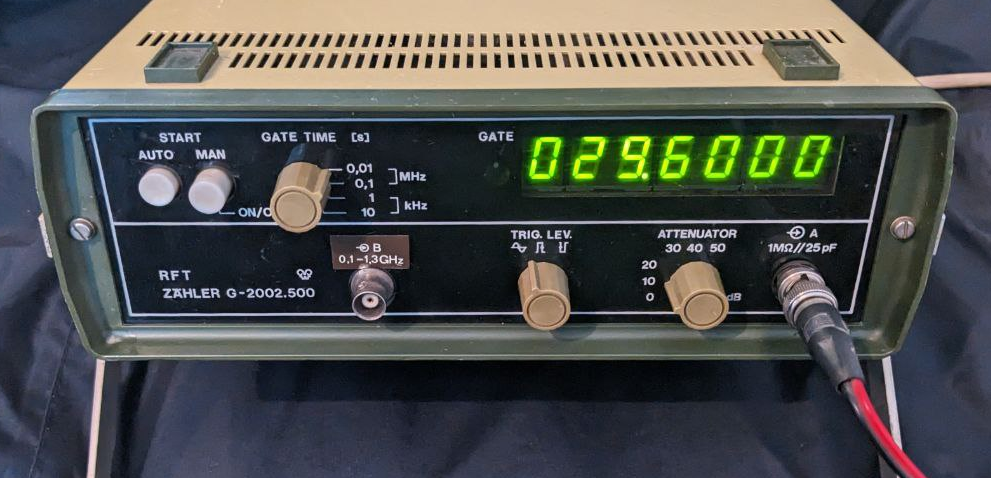
\includegraphics[width=0.85\textwidth]{foto/150}
    \caption{\scriptsize Frequenzzähler, der \qty{29,6}{\mega\hertz} misst}
    \label{frequenz_frequenzzaehler}
\end{figure}

    \end{column}
   \begin{column}{0.48\textwidth}
       \begin{itemize}
  \item Die genaue Sendefrequenz muss bekannt sein
  \item Die Messung erfolgt mit einem Frequenzzähler
  \item Zum Abgleich der Anzeige am Funkgerät
  \end{itemize}

   \end{column}
\end{columns}

\end{frame}

\begin{frame}
\only<1>{
\begin{QQuestion}{NI301}{Mit welchem Gerät kann die Sendefrequenz eines Senders gemessen werden?  }{Frequenzzähler}
{SWR-Meter}
{HF-Voltmeter}
{S-Meter}
\end{QQuestion}

}
\only<2>{
\begin{QQuestion}{NI301}{Mit welchem Gerät kann die Sendefrequenz eines Senders gemessen werden?  }{\textbf{\textcolor{DARCgreen}{Frequenzzähler}}}
{SWR-Meter}
{HF-Voltmeter}
{S-Meter}
\end{QQuestion}

}
\end{frame}%ENDCONTENT


\section{Sinusschwingung}
\label{section:sinusschwingung}
\begin{frame}%STARTCONTENT

\begin{columns}
    \begin{column}{0.48\textwidth}
    
\begin{figure}
    \DARCimage{0.85\linewidth}{725include}
    \caption{\scriptsize Die Spannung des Stromnetzes im zeitlichen Verlauf. Da die Spannung nicht die ganze Zeit den Höchstwert von \qty{325}{\volt} aufweist, wirkt sie effektiv übrigens nur mit \qty{230}{\volt}.}
    \label{n_frequenz_sinusschwingung}
\end{figure}


    \end{column}
   \begin{column}{0.48\textwidth}
       \begin{itemize}
  \item Die Wechselspannung aus dem Stromnetz schwingt nicht direkt zurück
  \item Es gibt einen sanften Übergang über 0
  \item Wie bei einem Pendel
  \item Diese Art der Schwingung ist eine Sinusschwingung
  \end{itemize}

   \end{column}
\end{columns}

\end{frame}

\begin{frame}
\begin{figure}
    \DARCimage{0.85\linewidth}{505include}
    \caption{\scriptsize Rechteckförmige Schwingung}
    \label{sinusschwingung_rechteck}
\end{figure}

\end{frame}

\begin{frame}
\begin{figure}
    \DARCimage{0.85\linewidth}{504include}
    \caption{\scriptsize Dreieckförmige Schwingung}
    \label{sinusschwingung_dreieck}
\end{figure}

\end{frame}

\begin{frame}
\begin{figure}
    \DARCimage{0.85\linewidth}{506include}
    \caption{\scriptsize Sägezahnförmige Schwingung}
    \label{sinusschwingung_saegezahn}
\end{figure}

\end{frame}

\begin{frame}
\only<1>{
\begin{question2x2}{NB401}{Welches Bild zeigt eine sinusförmige Wechselspannung?}{\DARCimage{1.0\linewidth}{505include}}
{\DARCimage{1.0\linewidth}{504include}}
{\DARCimage{1.0\linewidth}{503include}}
{\DARCimage{1.0\linewidth}{506include}}
\end{question2x2}

}
\only<2>{
\begin{question2x2}{NB401}{Welches Bild zeigt eine sinusförmige Wechselspannung?}{\DARCimage{1.0\linewidth}{505include}}
{\DARCimage{1.0\linewidth}{504include}}
{\textbf{\textcolor{DARCgreen}{\DARCimage{1.0\linewidth}{503include}}}}
{\DARCimage{1.0\linewidth}{506include}}
\end{question2x2}

}
\end{frame}%ENDCONTENT


\section{Amplitude und Periode}
\label{section:amplitude_periode}
\begin{frame}%STARTCONTENT

\frametitle{Amplitude}
\begin{columns}
    \begin{column}{0.48\textwidth}
    
\begin{figure}
    \DARCimage{0.85\linewidth}{726include}
    \caption{\scriptsize  Amplitude einer Sinusschwingung}
    \label{amplitude_periode_amplitudee}
\end{figure}


    \end{column}
   \begin{column}{0.48\textwidth}
       Der maximale Abstand von der Nulllinie zum höchsten oder tiefsten Punkt heißt \emph{Amplitude}


   \end{column}
\end{columns}

\end{frame}

\begin{frame}
\only<1>{
\begin{PQuestion}{NB404}{Was ist im Oszillogramm mit 1 markiert?}{Periode}
{Frequenz}
{Amplitude}
{Wellenlänge}
{\DARCimage{1.0\linewidth}{627include}}\end{PQuestion}

}
\only<2>{
\begin{PQuestion}{NB404}{Was ist im Oszillogramm mit 1 markiert?}{Periode}
{Frequenz}
{\textbf{\textcolor{DARCgreen}{Amplitude}}}
{Wellenlänge}
{\DARCimage{1.0\linewidth}{627include}}\end{PQuestion}

}
\end{frame}

\begin{frame}
\frametitle{Halbwellen}
\begin{columns}
    \begin{column}{0.48\textwidth}
    
\begin{figure}
    \DARCimage{0.85\linewidth}{727include}
    \caption{\scriptsize Positive und negative Halbwellen einer Sinusschwingung}
    \label{amplitude_periode_halbwellen}
\end{figure}


    \end{column}
   \begin{column}{0.48\textwidth}
       Bei einer Sinusschwingung gibt es positive und negative \emph{Halbwellen}


   \end{column}
\end{columns}

\end{frame}

\begin{frame}
\frametitle{Periode}
\begin{columns}
    \begin{column}{0.48\textwidth}
    
\begin{figure}
    \DARCimage{0.85\linewidth}{728include}
    \caption{\scriptsize Perioden einer Sinusschwingung}
    \label{amplitude_periode_perioden}
\end{figure}


    \end{column}
   \begin{column}{0.48\textwidth}
       Die Zeit ($t$) vom Beginn einer positiven Halbwelle bis zum Ende der darauf folgenden negativen Halbwelle heißt \emph{Periode} oder \emph{Periodendauer}


   \end{column}
\end{columns}

\end{frame}

\begin{frame}
\frametitle{Interaktiv}

\end{frame}

\begin{frame}
\only<1>{
\begin{PQuestion}{NB405}{Was ist im Oszillogramm mit 2 markiert?}{Spannung}
{Amplitude}
{Strom}
{Periode}
{\DARCimage{1.0\linewidth}{627include}}\end{PQuestion}

}
\only<2>{
\begin{PQuestion}{NB405}{Was ist im Oszillogramm mit 2 markiert?}{Spannung}
{Amplitude}
{Strom}
{\textbf{\textcolor{DARCgreen}{Periode}}}
{\DARCimage{1.0\linewidth}{627include}}\end{PQuestion}

}
 \end{frame}

\begin{frame}
\only<1>{
\begin{QQuestion}{NA213}{Welche Aussage ist für eine Schwingung von \num{145000000} Perioden pro Sekunde richtig?}{Ihre Ausbreitungsgeschwindigkeit beträgt \qty{145}{\km}/s.}
{Ihre Periodendauer beträgt \qty{145}{\us}.}
{Ihre Amplitude beträgt \qty{145}{\pps}.}
{Ihre Frequenz beträgt \qty{145}{\MHz}.}
\end{QQuestion}

}
\only<2>{
\begin{QQuestion}{NA213}{Welche Aussage ist für eine Schwingung von \num{145000000} Perioden pro Sekunde richtig?}{Ihre Ausbreitungsgeschwindigkeit beträgt \qty{145}{\km}/s.}
{Ihre Periodendauer beträgt \qty{145}{\us}.}
{Ihre Amplitude beträgt \qty{145}{\pps}.}
{\textbf{\textcolor{DARCgreen}{Ihre Frequenz beträgt \qty{145}{\MHz}.}}}
\end{QQuestion}

}

\end{frame}%ENDCONTENT


\section{Funkwellen}
\label{section:funkwellen}
\begin{frame}%STARTCONTENT

\frametitle{Antenne}
\begin{itemize}
  \item Eine elektrische Schwingung an einer Antenne wird als Funkwelle abgestrahlt
  \item Funkwellen sind elektromagnetische Wellen
  \item Sie breiten sich mit Lichtgeschwindigkeit aus
  \item Lichtgeschwindigkeit im Freiraum: etwa 300.000 Kilometer pro Sekunde
  \end{itemize}
\end{frame}

\begin{frame}
\only<1>{
\begin{QQuestion}{NB301}{Die Ausbreitungsgeschwindigkeit elektromagnetischer Wellen beträgt im Freiraum etwa~...}{\qty{3000000}{\km}/s.}
{\qty{300000}{\km}/s.}
{\qty{30000}{\km}/s.}
{\qty{3000}{\km}/s.}
\end{QQuestion}

}
\only<2>{
\begin{QQuestion}{NB301}{Die Ausbreitungsgeschwindigkeit elektromagnetischer Wellen beträgt im Freiraum etwa~...}{\qty{3000000}{\km}/s.}
{\textbf{\textcolor{DARCgreen}{\qty{300000}{\km}/s.}}}
{\qty{30000}{\km}/s.}
{\qty{3000}{\km}/s.}
\end{QQuestion}

}
\end{frame}

\begin{frame}
\frametitle{Funkwellen}
\begin{itemize}
  \item Bestehen aus Wellenbergen und Wellentälern
  \item Stellen die Stärke des Funksignals dar
  \item Das entspricht der \emph{Feldstärke}
  \end{itemize}

\end{frame}

\begin{frame}
\only<1>{
\begin{PQuestion}{NB402}{Was ist in der dargestellten Momentaufnahme einer Welle mit 1 markiert?}{Amplitude}
{Frequenz}
{Periode}
{Wellenlänge}
{\DARCimage{1.0\linewidth}{628include}}\end{PQuestion}

}
\only<2>{
\begin{PQuestion}{NB402}{Was ist in der dargestellten Momentaufnahme einer Welle mit 1 markiert?}{\textbf{\textcolor{DARCgreen}{Amplitude}}}
{Frequenz}
{Periode}
{Wellenlänge}
{\DARCimage{1.0\linewidth}{628include}}\end{PQuestion}

}
\end{frame}%ENDCONTENT


\section{Wellenlänge}
\label{section:wellenlaenge}
\begin{frame}%STARTCONTENT

\frametitle{Wellenlänge}
\begin{itemize}
  \item Der Abstand zwischen zwei gleichen Durchläufen einer Welle heißt \emph{Wellenlänge}
  \item Je größer die Frequenz, desto kleiner die Wellenlänge
  \end{itemize}
    \pause
    Die Wellenlänge wird mit dem griechischen Buchstaben $\lambda$ (Lambda) angegeben und in Meter ($m$) gemessen.



\end{frame}

\begin{frame}
\only<1>{
\begin{PQuestion}{NB403}{Was ist in der dargestellten Momentaufnahme einer Welle mit 2 markiert?}{Wellenlänge}
{Amplitude}
{Spannung}
{Strom}
{\DARCimage{1.0\linewidth}{628include}}\end{PQuestion}

}
\only<2>{
\begin{PQuestion}{NB403}{Was ist in der dargestellten Momentaufnahme einer Welle mit 2 markiert?}{\textbf{\textcolor{DARCgreen}{Wellenlänge}}}
{Amplitude}
{Spannung}
{Strom}
{\DARCimage{1.0\linewidth}{628include}}\end{PQuestion}

}
 \end{frame}

\begin{frame}
\only<1>{
\begin{QQuestion}{NA205}{Welche Einheit wird üblicherweise für die Wellenlänge verwendet?}{Meter pro Sekunde (m/s)}
{Meter (m)}
{Hertz (Hz)}
{Sekunde pro Meter (s/m)}
\end{QQuestion}

}
\only<2>{
\begin{QQuestion}{NA205}{Welche Einheit wird üblicherweise für die Wellenlänge verwendet?}{Meter pro Sekunde (m/s)}
{\textbf{\textcolor{DARCgreen}{Meter (m)}}}
{Hertz (Hz)}
{Sekunde pro Meter (s/m)}
\end{QQuestion}

}
 \end{frame}

\begin{frame}
\frametitle{Zusammenhang Frequenz – Wellenlänge}
\begin{itemize}
  \item Über die Lichtgeschwindigkeit
  \item Eine Welle mit einer Frequenz von \qty{1}{\hertz} breitet sich 300.\qty{000}{\kilo\metre} aus bevor der nächste Durchlauf beginnt
  \item Bei \qty{1000}{\hertz} sind es nur \qty{300}{\kilo\metre}
  \item Bei \qty{1}{\mega\hertz} sind es \qty{300}{\metre}
  \end{itemize}

\end{frame}

\begin{frame}$f[\textrm{MHz}] = \dfrac{300}{\lambda[\textrm{m}]} \quad\quad\quad \lambda[\textrm{m}] = \dfrac{300}{f[\textrm{MHz}]}$

\end{frame}

\begin{frame}
\frametitle{Beispiele}
Wellenlänge aus Frequenz

$\lambda[\text{m}] = \dfrac{300}{f[\text{MHz}]} = \dfrac{300}{145,3 \ \text{MHz}} \approx 2,06 \ \text{m}$
    \pause
    Frequenz aus Wellenlänge

$f[\text{MHz}] = \dfrac{300}{\lambda[\text{m}]} = \dfrac{300}{2,06 \ \text{m}} \approx 145,3 \ \text{MHz}$



\end{frame}

\begin{frame}
\frametitle{Band}
Statt der Frequenz wird häufig das gerundete Band angegeben

\begin{table}
\begin{DARCtabular}{lll}
     Frequenz  & Wellenlänge  & Band   \\
     \qty{28}{\mega\hertz} -- \qty{29,7}{\mega\hertz}  & \qty{10,7}{\metre} -- \qty{10,1}{\metre}  & \qty{10}{\metre}-Band   \\
     \qty{144}{\mega\hertz} -- \qty{146}{\mega\hertz}  & \qty{2,08}{\metre} -- \qty{2,05}{\metre}  & \qty{2}{\metre}-Band   \\
     \qty{430}{\mega\hertz} -- \qty{440}{\mega\hertz}  & \qty{68}{\centi\metre} -- \qty{70}{\centi\metre}  & \qty{70}{\centi\metre}-Band   \\
\end{DARCtabular}
\caption{Die drei Amateurfunkbänder, die für alle Klassen freigegeben sind}
\label{n_funkwellen_baender}
\end{table}
\end{frame}

\begin{frame}
\only<1>{
\begin{QQuestion}{NB302}{Welcher Frequenz $f$ entspricht in etwa eine Wellenlänge von \qty{2,08}{\m} im Freiraum?}{\qty{149}{\MHz}}
{\qty{144}{\MHz}}
{\qty{433}{\MHz}}
{\qty{437}{\MHz}}
\end{QQuestion}

}
\only<2>{
\begin{QQuestion}{NB302}{Welcher Frequenz $f$ entspricht in etwa eine Wellenlänge von \qty{2,08}{\m} im Freiraum?}{\qty{149}{\MHz}}
{\textbf{\textcolor{DARCgreen}{\qty{144}{\MHz}}}}
{\qty{433}{\MHz}}
{\qty{437}{\MHz}}
\end{QQuestion}

}
\end{frame}

\begin{frame}
\only<1>{
\begin{QQuestion}{NB303}{Welcher Wellenlänge $\lambda$ entspricht in etwa eine Frequenz von \qty{433,500}{\MHz} im Freiraum?}{\qty{2,06}{\m}}
{\qty{58,0}{\cm}}
{\qty{0,69}{\m}}
{\qty{198}{\cm}}
\end{QQuestion}

}
\only<2>{
\begin{QQuestion}{NB303}{Welcher Wellenlänge $\lambda$ entspricht in etwa eine Frequenz von \qty{433,500}{\MHz} im Freiraum?}{\qty{2,06}{\m}}
{\qty{58,0}{\cm}}
{\textbf{\textcolor{DARCgreen}{\qty{0,69}{\m}}}}
{\qty{198}{\cm}}
\end{QQuestion}

}
\end{frame}%ENDCONTENT


\section{Wasserfalldiagramm}
\label{section:wasserfall}
\begin{frame}%STARTCONTENT

\frametitle{Empfang}
\begin{itemize}
  \item Frequenz wird am Funkgerät über Drehknopf oder Tasten eingestellt
  \item Es können nur Stationen auf der eingestellten Frequenz gehört werden
  \item Langsam \enquote{über das Band drehen}, um andere Stationen zu hören
  \end{itemize}
\end{frame}

\begin{frame}
\frametitle{Amplitudenspektrum und Wassefalldiagramm}
\begin{columns}
    \begin{column}{0.48\textwidth}
    
\begin{figure}
    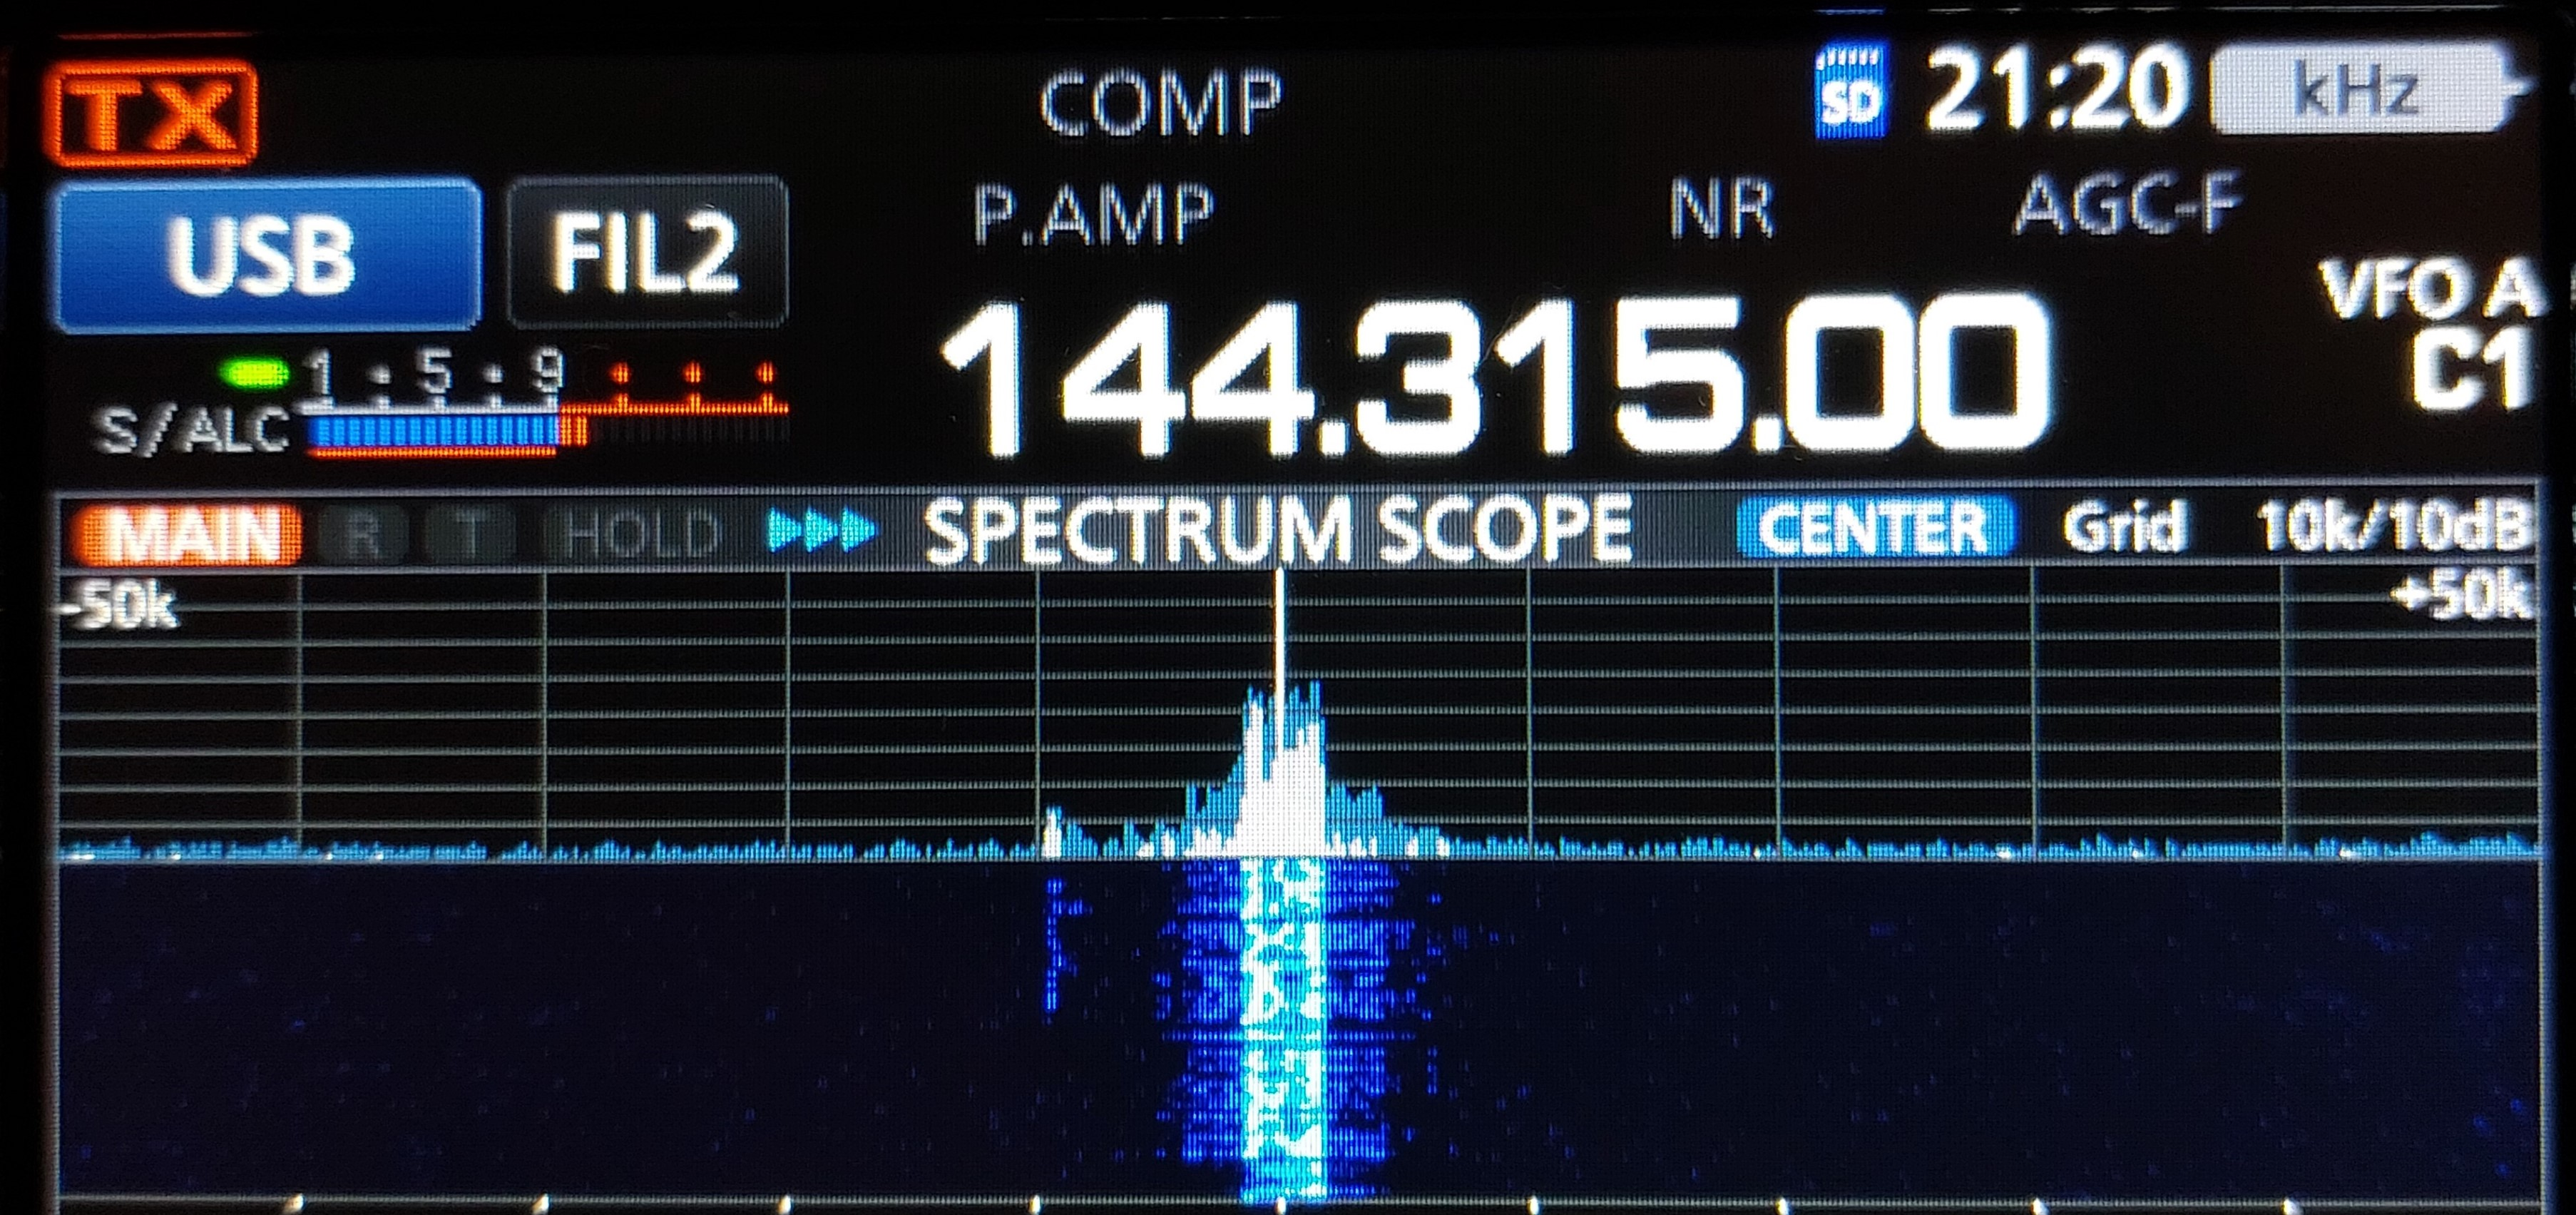
\includegraphics[width=0.85\textwidth]{foto/95}
    \caption{\scriptsize Display eines ICOM IC-9700 mit Frequenzanzeige, Amplitudenspektrum und Wasserfalldiagramm. Eine starke Station wird empfangen.}
    \label{n_wasserfall_starke_station}
\end{figure}

    \end{column}
   \begin{column}{0.48\textwidth}
       \begin{itemize}
  \item Moderne Funkgeräte
  \item Anzeige weiterer sendender Stationen ober- und unterhalb der eingestellten Frequenz
  \end{itemize}

   \end{column}
\end{columns}

\end{frame}

\begin{frame}
\frametitle{Amplitudenspektrum}
\begin{columns}
    \begin{column}{0.48\textwidth}
    
\begin{figure}
    \includegraphics[width=0.85\textwidth]{foto/135}
    \caption{\scriptsize Display eines ICOM IC-9700. Hervorgehoben ist das Amplitudenspektrum}
    \label{n_wasserfall_amplitudenspektrum}
\end{figure}

    \end{column}
   \begin{column}{0.48\textwidth}
       \begin{itemize}
  \item Amplitude umso höher je stärker das Signal ist
  \item Weitere Stationen sind im Amplitudenspektrum sichtbar
  \end{itemize}

   \end{column}
\end{columns}

\end{frame}

\begin{frame}
\frametitle{Wasserfalldiagramm}
\begin{columns}
    \begin{column}{0.48\textwidth}
    
\begin{figure}
    \includegraphics[width=0.85\textwidth]{foto/136}
    \caption{\scriptsize Display eines ICOM IC-9700. Hervorgehoben ist der Wasserfall}
    \label{n_wasserfall_wasserfall}
\end{figure}

    \end{column}
   \begin{column}{0.48\textwidth}
       \begin{itemize}
  \item Zeitlicher Verlauf auf senkrechter Achse
  \item Farbton oder Helligkeit zeigt die Stärke des Signals
  \item Läuft von oben nach unten durch
  \item Beginn und Ende einer Aussendung erkennbar
  \end{itemize}

   \end{column}
\end{columns}

\end{frame}

\begin{frame}
\only<1>{
\begin{PQuestion}{NF104}{Die Darstellung zeigt das Display eines Transceivers. Wie wird die Anzeige 3 bezeichnet?}{Power-Meter}
{Amplitudenspektrum}
{S-Meter}
{Wasserfalldiagramm}
{\DARCimage{1.0\linewidth}{578include}}\end{PQuestion}

}
\only<2>{
\begin{PQuestion}{NF104}{Die Darstellung zeigt das Display eines Transceivers. Wie wird die Anzeige 3 bezeichnet?}{Power-Meter}
{\textbf{\textcolor{DARCgreen}{Amplitudenspektrum}}}
{S-Meter}
{Wasserfalldiagramm}
{\DARCimage{1.0\linewidth}{578include}}\end{PQuestion}

}
\end{frame}

\begin{frame}
\only<1>{
\begin{PQuestion}{NF105}{Die Darstellung zeigt das Display eines Transceivers. Wie wird die Anzeige 4 bezeichnet?}{Regenbogendiagramm}
{Wasserfalldiagramm}
{SWR-Meter}
{Power-Meter}
{\DARCimage{1.0\linewidth}{578include}}\end{PQuestion}

}
\only<2>{
\begin{PQuestion}{NF105}{Die Darstellung zeigt das Display eines Transceivers. Wie wird die Anzeige 4 bezeichnet?}{Regenbogendiagramm}
{\textbf{\textcolor{DARCgreen}{Wasserfalldiagramm}}}
{SWR-Meter}
{Power-Meter}
{\DARCimage{1.0\linewidth}{578include}}\end{PQuestion}

}
\end{frame}

\begin{frame}
\only<1>{
\begin{PQuestion}{NF106}{Die Darstellung zeigt das Display eines Transceivers. Was wird im Wasserfalldiagramm dargestellt und wie erfolgt die Darstellung?}{Frequenz und Zeit auf den Achsen und Signalstärke als Farbton und/oder Helligkeit.}
{Frequenz und Signalstärke auf den Achsen und Zeit als Farbton und/oder Helligkeit.}
{Signalstärke und Zeit auf den Achsen und Frequenz als Farbton und/oder Helligkeit.}
{Signalstärke und Phase auf den Achsen und Zeit als Farbton und/oder Helligkeit.}
{\DARCimage{1.0\linewidth}{579include}}\end{PQuestion}

}
\only<2>{
\begin{PQuestion}{NF106}{Die Darstellung zeigt das Display eines Transceivers. Was wird im Wasserfalldiagramm dargestellt und wie erfolgt die Darstellung?}{\textbf{\textcolor{DARCgreen}{Frequenz und Zeit auf den Achsen und Signalstärke als Farbton und/oder Helligkeit.}}}
{Frequenz und Signalstärke auf den Achsen und Zeit als Farbton und/oder Helligkeit.}
{Signalstärke und Zeit auf den Achsen und Frequenz als Farbton und/oder Helligkeit.}
{Signalstärke und Phase auf den Achsen und Zeit als Farbton und/oder Helligkeit.}
{\DARCimage{1.0\linewidth}{579include}}\end{PQuestion}

}
\end{frame}

\begin{frame}
\frametitle{Unterschied Oszillogramm und Amplitudenspektrum}
\begin{itemize}
  \item Amplitudenspektrum zeigt horizontal Amplituden für verschiedene Frequenzen an
  \item Oszillogramm zeigt horizontal Amplituden zu verschiedenen Zeitpunkten an
  \end{itemize}
\end{frame}

\begin{frame}
\only<1>{
\begin{QQuestion}{NI401}{Was ist der Unterschied zwischen einem Oszillogramm und einem Amplitudenspektrum?}{Ein Oszillogramm zeigt den Strom und ein Amplitudenspektrum die Spannung eines Signals.}
{Ein Oszillogramm zeigt die Frequenzanteile und ein Amplitudenspektrum einen zeitlichen Verlauf eines Signals.}
{Ein Oszillogramm zeigt die Spannung und ein Amplitudenspektrum den Strom eines Signals.}
{Ein Oszillogramm zeigt einen zeitlichen Verlauf und ein Amplitudenspektrum die Frequenzanteile eines Signals.}
\end{QQuestion}

}
\only<2>{
\begin{QQuestion}{NI401}{Was ist der Unterschied zwischen einem Oszillogramm und einem Amplitudenspektrum?}{Ein Oszillogramm zeigt den Strom und ein Amplitudenspektrum die Spannung eines Signals.}
{Ein Oszillogramm zeigt die Frequenzanteile und ein Amplitudenspektrum einen zeitlichen Verlauf eines Signals.}
{Ein Oszillogramm zeigt die Spannung und ein Amplitudenspektrum den Strom eines Signals.}
{\textbf{\textcolor{DARCgreen}{Ein Oszillogramm zeigt einen zeitlichen Verlauf und ein Amplitudenspektrum die Frequenzanteile eines Signals.}}}
\end{QQuestion}

}
\end{frame}%ENDCONTENT


\section{Frequenzspektrum}
\label{section:frequenzspektrum}
\begin{frame}%STARTCONTENT

\begin{figure}
    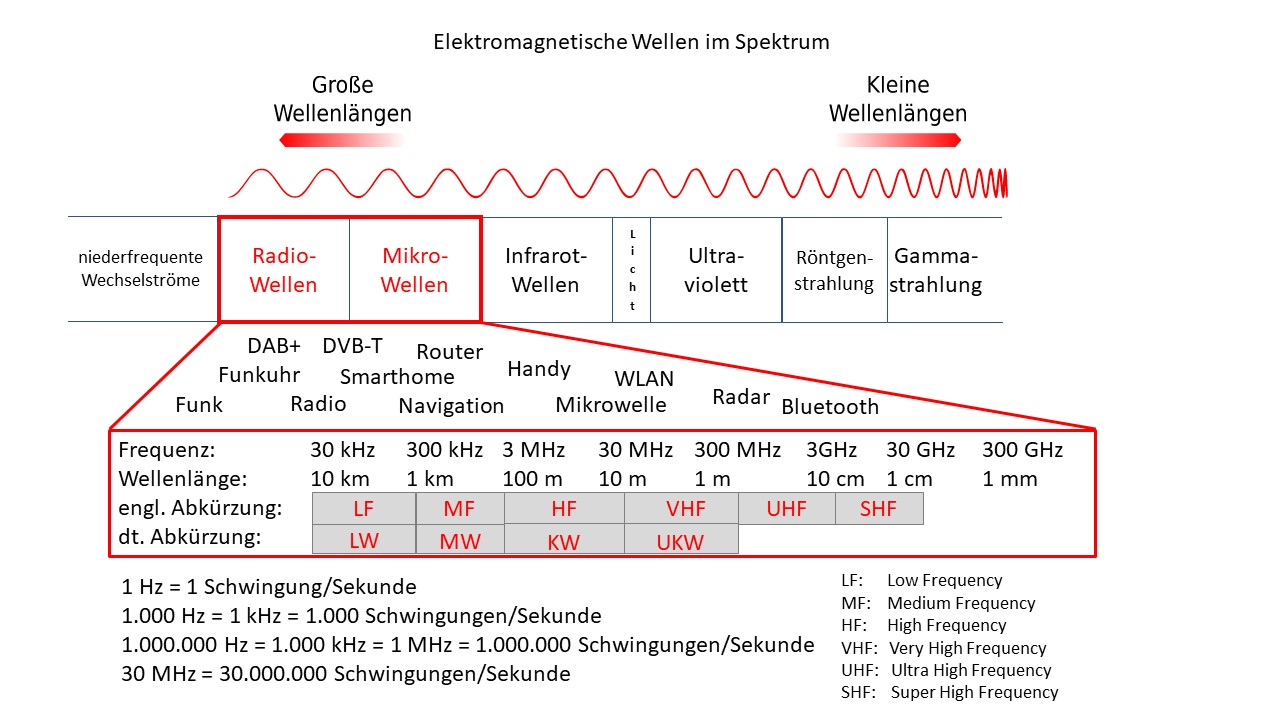
\includegraphics[width=0.85\textwidth]{foto/94}
    \caption{\scriptsize Spektrum der elektromagnetischen Wellen}
    \label{n_frequenzspektrum}
\end{figure}

\end{frame}

\begin{frame}\begin{table}
\begin{DARCtabular}{rcrXl}
     \qty{30}{\kilo\hertz}  & --  & \qty{300}{\kilo\hertz}  & Low Frequency  & LF   \\
      &  &  & (Langwelle)  & (LW)   \\
     \qty{300}{\kilo\hertz}  & --  & \qty{3000}{\kilo\hertz}  & Medium Frequency  & MF   \\
      &  &  & (Mittelwelle)  & (MW)   \\
     \qty{3}{\mega\hertz}  & --  & \qty{30}{\mega\hertz}  & \emph{High Frequency}  & \emph{HF}   \\
      &  &  & Short Wave  & SW   \\
      &  &  & (Kurzwelle)  & (KW)   \\
     \qty{30}{\mega\hertz}  & --  & \qty{300}{\mega\hertz}  & \emph{Very High Frequency}  & \emph{VHF}   \\
      &  &  & (Ultrakurzwelle)  & (UKW)   \\
     \qty{300}{\mega\hertz}  & --  & \qty{3000}{\mega\hertz}  & \emph{Ultra High Frequency}  & \emph{UHF}   \\
      &  &  & (Dezimeterwelle)  &   \\
     \qty{3}{\giga\hertz}  & --  & \qty{30}{\giga\hertz}  & Super High Frequency  & SHF   \\
     \qty{30}{\giga\hertz}  & --  & \qty{300}{\giga\hertz}  & Extemely High Frequency  & EHF   \\
\end{DARCtabular}
\caption{Die Frequenzbereiche von 30 kHz bis 300 GHz und ihre üblichen Bezeichnungen.}
\label{n_frequenzspektrum_bereiche}
\end{table}
\end{frame}

\begin{frame}
\only<1>{
\begin{QQuestion}{BC104}{Wie wird der Frequenzbereich von \qtyrange{3}{30}{\MHz} bezeichnet?}{Medium Frequency (MF) oder Mittelwelle (MW)}
{Very High Frequency (VHF) oder Ultrakurzwelle (UKW)}
{Ultra High Frequency (UHF) oder Dezimeterwelle}
{High Frequency (HF), Short Wave (SW) oder Kurzwelle (KW)}
\end{QQuestion}

}
\only<2>{
\begin{QQuestion}{BC104}{Wie wird der Frequenzbereich von \qtyrange{3}{30}{\MHz} bezeichnet?}{Medium Frequency (MF) oder Mittelwelle (MW)}
{Very High Frequency (VHF) oder Ultrakurzwelle (UKW)}
{Ultra High Frequency (UHF) oder Dezimeterwelle}
{\textbf{\textcolor{DARCgreen}{High Frequency (HF), Short Wave (SW) oder Kurzwelle (KW)}}}
\end{QQuestion}

}
\end{frame}

\begin{frame}
\only<1>{
\begin{QQuestion}{BC105}{Wie wird der Frequenzbereich zwischen \qtyrange{30}{300}{\MHz} bezeichnet?}{High Frequency (HF), Short Wave (SW) oder Kurzwelle (KW)}
{Ultra High Frequency (UHF) oder Dezimeterwelle}
{Very High Frequency (VHF) oder Ultrakurzwelle (UKW)}
{Medium Frequency (MF) oder Mittelwelle (MW)}
\end{QQuestion}

}
\only<2>{
\begin{QQuestion}{BC105}{Wie wird der Frequenzbereich zwischen \qtyrange{30}{300}{\MHz} bezeichnet?}{High Frequency (HF), Short Wave (SW) oder Kurzwelle (KW)}
{Ultra High Frequency (UHF) oder Dezimeterwelle}
{\textbf{\textcolor{DARCgreen}{Very High Frequency (VHF) oder Ultrakurzwelle (UKW)}}}
{Medium Frequency (MF) oder Mittelwelle (MW)}
\end{QQuestion}

}
\end{frame}

\begin{frame}
\only<1>{
\begin{QQuestion}{BC106}{Wie wird der Frequenzbereich zwischen \qtyrange{300}{3000}{\MHz} bezeichnet?}{Very High Frequency (VHF) oder Ultrakurzwelle (UKW)}
{Ultra High Frequency (UHF) oder Dezimeterwelle}
{High Frequency (HF), Short Wave (SW) oder Kurzwelle (KW)}
{Medium Frequency (MF) oder Mittelwelle (MW)}
\end{QQuestion}

}
\only<2>{
\begin{QQuestion}{BC106}{Wie wird der Frequenzbereich zwischen \qtyrange{300}{3000}{\MHz} bezeichnet?}{Very High Frequency (VHF) oder Ultrakurzwelle (UKW)}
{\textbf{\textcolor{DARCgreen}{Ultra High Frequency (UHF) oder Dezimeterwelle}}}
{High Frequency (HF), Short Wave (SW) oder Kurzwelle (KW)}
{Medium Frequency (MF) oder Mittelwelle (MW)}
\end{QQuestion}

}
\end{frame}

\begin{frame}
\only<1>{
\begin{QQuestion}{BC101}{Wie wird der Frequenzbereich bezeichnet, in dem sich das \qty{10}{\m}-Band befindet?}{Ultra High Frequency (UHF) oder Dezimeterwelle}
{Very High Frequency (VHF) oder Ultrakurzwelle (UKW)}
{High Frequency (HF), Short Wave (SW) oder Kurzwelle (KW)}
{Medium Frequency (MF) oder Mittelwelle (MW)}
\end{QQuestion}

}
\only<2>{
\begin{QQuestion}{BC101}{Wie wird der Frequenzbereich bezeichnet, in dem sich das \qty{10}{\m}-Band befindet?}{Ultra High Frequency (UHF) oder Dezimeterwelle}
{Very High Frequency (VHF) oder Ultrakurzwelle (UKW)}
{\textbf{\textcolor{DARCgreen}{High Frequency (HF), Short Wave (SW) oder Kurzwelle (KW)}}}
{Medium Frequency (MF) oder Mittelwelle (MW)}
\end{QQuestion}

}

\end{frame}

\begin{frame}
\only<1>{
\begin{QQuestion}{BC102}{Wie wird der Frequenzbereich bezeichnet, in dem sich das \qty{2}{\m}-Band befindet?}{High Frequency (HF), Short Wave (SW) oder Kurzwelle (KW)}
{Ultra High Frequency (UHF) oder Dezimeterwelle}
{Very High Frequency (VHF) oder Ultrakurzwelle (UKW)}
{Medium Frequency (MF) oder Mittelwelle (MW)}
\end{QQuestion}

}
\only<2>{
\begin{QQuestion}{BC102}{Wie wird der Frequenzbereich bezeichnet, in dem sich das \qty{2}{\m}-Band befindet?}{High Frequency (HF), Short Wave (SW) oder Kurzwelle (KW)}
{Ultra High Frequency (UHF) oder Dezimeterwelle}
{\textbf{\textcolor{DARCgreen}{Very High Frequency (VHF) oder Ultrakurzwelle (UKW)}}}
{Medium Frequency (MF) oder Mittelwelle (MW)}
\end{QQuestion}

}

\end{frame}

\begin{frame}
\only<1>{
\begin{QQuestion}{BC103}{Wie wird der Frequenzbereich bezeichnet, in dem sich das \qty{70}{\cm}-Band befindet?}{Ultra High Frequency (UHF) oder Dezimeterwelle}
{Very High Frequency (VHF) oder Ultrakurzwelle (UKW)}
{High Frequency (HF), Short Wave (SW) oder Kurzwelle (KW)}
{Medium Frequency (MF) oder Mittelwelle (MW)}
\end{QQuestion}

}
\only<2>{
\begin{QQuestion}{BC103}{Wie wird der Frequenzbereich bezeichnet, in dem sich das \qty{70}{\cm}-Band befindet?}{\textbf{\textcolor{DARCgreen}{Ultra High Frequency (UHF) oder Dezimeterwelle}}}
{Very High Frequency (VHF) oder Ultrakurzwelle (UKW)}
{High Frequency (HF), Short Wave (SW) oder Kurzwelle (KW)}
{Medium Frequency (MF) oder Mittelwelle (MW)}
\end{QQuestion}

}

\end{frame}%ENDCONTENT


\section{Frequenzzuteilung}
\label{section:frequenzzuteilung}
\begin{frame}%STARTCONTENT
\begin{itemize}
  \item Jede Frequenznutzung bedarf einer vorherigen \emph{Frequenzzuteilung}
  \item Verankert im Telekommunikationsgesetz (TKG)
  \item Einzelzuteilung oder Allgemeinzuteilung
  \end{itemize}

\end{frame}

\begin{frame}\begin{itemize}
  \item Amateurfunk darf nur auf den zugeteilten Frequenzen durchgeführt werden
  \item Frequenzbereiche sind zwar international vereinbart
  \item \emph{Aber} die nationalen Bestimmungen sind maßgebend
  \end{itemize}
\end{frame}

\begin{frame}
\only<1>{
\begin{QQuestion}{VE102}{Bedarf jede Frequenznutzung einer Frequenzzuteilung?}{Eine Frequenznutzung ist auch ohne Frequenzzuteilung zulässig.}
{Erst ab \qty{0,1}{\W} ist eine Frequenzzuteilung erforderlich.}
{Es gibt Ausnahmen von der Notwendigkeit zur Frequenzzuteilung, z.~B. die ISM-Frequenzen.}
{Jede Frequenznutzung bedarf einer vorherigen Frequenzzuteilung.}
\end{QQuestion}

}
\only<2>{
\begin{QQuestion}{VE102}{Bedarf jede Frequenznutzung einer Frequenzzuteilung?}{Eine Frequenznutzung ist auch ohne Frequenzzuteilung zulässig.}
{Erst ab \qty{0,1}{\W} ist eine Frequenzzuteilung erforderlich.}
{Es gibt Ausnahmen von der Notwendigkeit zur Frequenzzuteilung, z.~B. die ISM-Frequenzen.}
{\textbf{\textcolor{DARCgreen}{Jede Frequenznutzung bedarf einer vorherigen Frequenzzuteilung.}}}
\end{QQuestion}

}
\end{frame}

\begin{frame}
\only<1>{
\begin{QQuestion}{VD701}{Darf ein Funkamateur in Deutschland alle in den Radio Regulations (RR) für den Amateurfunkdienst zugewiesenen Frequenzbereiche benutzen?}{Nein, es dürfen nur Frequenzen genutzt werden, die durch nationale Regelungen umgesetzt wurden.}
{Ja, weil die internationalen Regelungen der Radio Regulations (RR) auch in Deutschland gelten.}
{Ja, wenn der Betrieb bei der Bundesnetzagentur vorher angemeldet wurde.}
{Nein, die in Deutschland zulässigen Frequenzbereiche ergeben sich aus der Frequenznutzungsplanaufstellungsverordnung.}
\end{QQuestion}

}
\only<2>{
\begin{QQuestion}{VD701}{Darf ein Funkamateur in Deutschland alle in den Radio Regulations (RR) für den Amateurfunkdienst zugewiesenen Frequenzbereiche benutzen?}{\textbf{\textcolor{DARCgreen}{Nein, es dürfen nur Frequenzen genutzt werden, die durch nationale Regelungen umgesetzt wurden.}}}
{Ja, weil die internationalen Regelungen der Radio Regulations (RR) auch in Deutschland gelten.}
{Ja, wenn der Betrieb bei der Bundesnetzagentur vorher angemeldet wurde.}
{Nein, die in Deutschland zulässigen Frequenzbereiche ergeben sich aus der Frequenznutzungsplanaufstellungsverordnung.}
\end{QQuestion}

}
\end{frame}

\begin{frame}
\only<1>{
\begin{QQuestion}{VC110}{Was gilt für Funkamateure hinsichtlich der Frequenznutzung? Ein Funkamateur darf mit seiner Amateurfunkstelle~...}{beliebige Frequenzen nutzen, sofern keine anderen Funkdienste gestört werden.}
{auf allen für seine ITU-Region zugelassenen Frequenzen senden.}
{auf den für den Amateurfunkdienst ausgewiesenen Frequenzen senden.}
{im Rahmen einer Notfunkübung auch auf nicht für den Amateurfunkdienst ausgewiesenen Frequenzen senden.}
\end{QQuestion}

}
\only<2>{
\begin{QQuestion}{VC110}{Was gilt für Funkamateure hinsichtlich der Frequenznutzung? Ein Funkamateur darf mit seiner Amateurfunkstelle~...}{beliebige Frequenzen nutzen, sofern keine anderen Funkdienste gestört werden.}
{auf allen für seine ITU-Region zugelassenen Frequenzen senden.}
{\textbf{\textcolor{DARCgreen}{auf den für den Amateurfunkdienst ausgewiesenen Frequenzen senden.}}}
{im Rahmen einer Notfunkübung auch auf nicht für den Amateurfunkdienst ausgewiesenen Frequenzen senden.}
\end{QQuestion}

}
\end{frame}

\begin{frame}
\frametitle{Frequenzbereiche für den Amateurfunkdienst}
\begin{itemize}
  \item Sind in Deutschland in der Anlage 1 der \emph{Verordnung über den Amateurfunk (AFuV)} geregelt
  \item Senden nur auf den der Zeugnisklasse zugewiesenen Frequenzen
  \item Weitere einzuhaltende Nutzungsbestimmungen
  \item Es gibt ergänzende bindende Verfügungen und Mitteilungen
  \item Werden im Amtsblatt und auf der Webseite der Bundesnetzagentur (BNetzA) veröffentlicht
  \end{itemize}
\end{frame}

\begin{frame}
\begin{figure}
    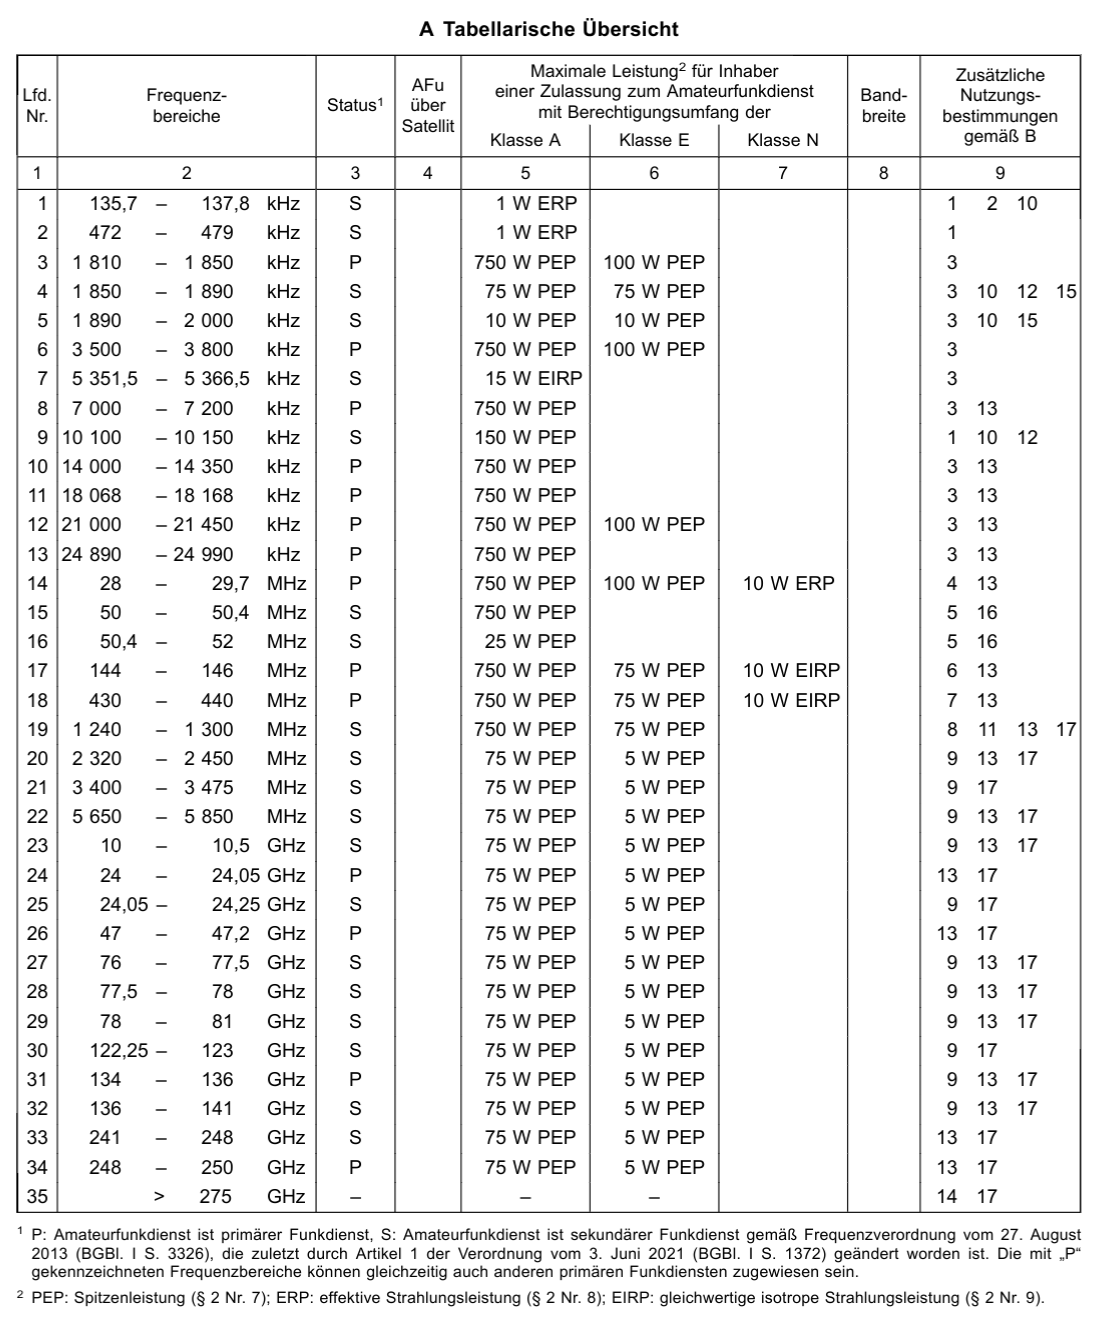
\includegraphics[width=0.85\textwidth]{foto/99}
    \caption{\scriptsize Tabellarische Übersicht, Anlage 1, AFuV (Korrektur in den Leistungen für Klasse~N notwendig)}
    \label{n_frequenzbereiche_afuv_anlage_1}
\end{figure}

\end{frame}

\begin{frame}
\only<1>{
\begin{QQuestion}{VD101}{Wo kann der Funkamateur nachschlagen, welche Frequenzbereiche er entsprechend seiner Zeugnisklasse in Deutschland nutzen darf?}{In der Anlage zur Frequenzverordnung (FreqV) und den dazugehörigen Mitteilungen der BNetzA}
{In den Radio Regulations (RR)}
{Im Amateurfunkgesetz (AFuG)}
{In der Anlage 1 der Amateurfunkverordnung (AFuV) und ggf. weiteren Mitteilungen der BNetzA}
\end{QQuestion}

}
\only<2>{
\begin{QQuestion}{VD101}{Wo kann der Funkamateur nachschlagen, welche Frequenzbereiche er entsprechend seiner Zeugnisklasse in Deutschland nutzen darf?}{In der Anlage zur Frequenzverordnung (FreqV) und den dazugehörigen Mitteilungen der BNetzA}
{In den Radio Regulations (RR)}
{Im Amateurfunkgesetz (AFuG)}
{\textbf{\textcolor{DARCgreen}{In der Anlage 1 der Amateurfunkverordnung (AFuV) und ggf. weiteren Mitteilungen der BNetzA}}}
\end{QQuestion}

}
\end{frame}

\begin{frame}
\only<1>{
\begin{QQuestion}{VD702}{Wo sind die für den Amateurfunkdienst in Deutschland ausgewiesenen Frequenzbereiche und die zugehörigen ausführlichen Nutzungsbedingungen zu finden?}{In Artikel~5 der Radio Regulations (RR)}
{In der Anlage 1 der Amateurfunkverordnung (AFuV) und ggf. weiteren Mitteilungen der BNetzA}
{Im Frequenzplan (FreqP)}
{In der Anlage zur Frequenzverordnung (FreqV)}
\end{QQuestion}

}
\only<2>{
\begin{QQuestion}{VD702}{Wo sind die für den Amateurfunkdienst in Deutschland ausgewiesenen Frequenzbereiche und die zugehörigen ausführlichen Nutzungsbedingungen zu finden?}{In Artikel~5 der Radio Regulations (RR)}
{\textbf{\textcolor{DARCgreen}{In der Anlage 1 der Amateurfunkverordnung (AFuV) und ggf. weiteren Mitteilungen der BNetzA}}}
{Im Frequenzplan (FreqP)}
{In der Anlage zur Frequenzverordnung (FreqV)}
\end{QQuestion}

}
\end{frame}%ENDCONTENT


\section{Amateurfunkbänder}
\label{section:amateurfunkbaender}
\begin{frame}%STARTCONTENT
\begin{itemize}
  \item Funkamateure müssen wissen, welche Frequenzen genutzt werden dürfen
  \item Lässt sich aus Anlage 1 AfuV ablesen
  \item Die Anlage 1 liegt in der Prüfung als Hilfsmittel bereit
  \end{itemize}
\end{frame}

\begin{frame}
\begin{figure}
    \DARCimage{0.85\linewidth}{829include}
    \caption{\scriptsize Frequenzbereiche im Amateurfunk unter \qty{300}{\mega\hertz}}
    \label{amateuerfunkbaender_2}
\end{figure}

\end{frame}

\begin{frame}
\begin{figure}
    \DARCimage{0.85\linewidth}{830include}
    \caption{\scriptsize Frequenzbereiche im Amateurfunk über \qty{300}{\mega\hertz}}
    \label{amateuerfunkbaender_1}
\end{figure}

\end{frame}

\begin{frame}
\only<1>{
\begin{QQuestion}{VD709}{Welche Antwort enthält die richtige Anfangs- und Endfrequenz für das \qty{160}{\m}-Amateurfunkband in Deutschland?}{\qtyrange{1810}{2000}{\kHz}}
{\qtyrange{1805}{1850}{\kHz}}
{\qtyrange{1800}{1900}{\kHz}}
{\qtyrange{1800}{1990}{\kHz}}
\end{QQuestion}

}
\only<2>{
\begin{QQuestion}{VD709}{Welche Antwort enthält die richtige Anfangs- und Endfrequenz für das \qty{160}{\m}-Amateurfunkband in Deutschland?}{\textbf{\textcolor{DARCgreen}{\qtyrange{1810}{2000}{\kHz}}}}
{\qtyrange{1805}{1850}{\kHz}}
{\qtyrange{1800}{1900}{\kHz}}
{\qtyrange{1800}{1990}{\kHz}}
\end{QQuestion}

}
\end{frame}

\begin{frame}
\only<1>{
\begin{QQuestion}{VD710}{Welche Antwort enthält die richtige Anfangs- und Endfrequenz für das \qty{80}{\m}-Amateurfunkband in Deutschland?}{\qtyrange{3,8}{4}{\MHz}}
{\qtyrange{3,5}{3,6}{\MHz}}
{\qtyrange{3,8}{3,9}{\MHz}}
{\qtyrange{3,5}{3,8}{\MHz}}
\end{QQuestion}

}
\only<2>{
\begin{QQuestion}{VD710}{Welche Antwort enthält die richtige Anfangs- und Endfrequenz für das \qty{80}{\m}-Amateurfunkband in Deutschland?}{\qtyrange{3,8}{4}{\MHz}}
{\qtyrange{3,5}{3,6}{\MHz}}
{\qtyrange{3,8}{3,9}{\MHz}}
{\textbf{\textcolor{DARCgreen}{\qtyrange{3,5}{3,8}{\MHz}}}}
\end{QQuestion}

}
\end{frame}

\begin{frame}
\only<1>{
\begin{QQuestion}{VD711}{Welche Antwort enthält die richtige Anfangs- und Endfrequenz für das \qty{40}{\m}-Amateurfunkband in Deutschland?}{\qtyrange{7}{7,3}{\MHz}}
{\qtyrange{7,1}{7,3}{\MHz}}
{\qtyrange{7}{7,2}{\MHz}}
{\qtyrange{7,1}{7,5}{\MHz}}
\end{QQuestion}

}
\only<2>{
\begin{QQuestion}{VD711}{Welche Antwort enthält die richtige Anfangs- und Endfrequenz für das \qty{40}{\m}-Amateurfunkband in Deutschland?}{\qtyrange{7}{7,3}{\MHz}}
{\qtyrange{7,1}{7,3}{\MHz}}
{\textbf{\textcolor{DARCgreen}{\qtyrange{7}{7,2}{\MHz}}}}
{\qtyrange{7,1}{7,5}{\MHz}}
\end{QQuestion}

}
\end{frame}

\begin{frame}
\only<1>{
\begin{QQuestion}{VD712}{Welche Antwort enthält die richtige Anfangs- und Endfrequenz für das \qty{30}{\m}-Amateurfunkband in Deutschland?}{\qtyrange{10}{10,25}{\MHz}}
{\qtyrange{10,1}{10,25}{\MHz}}
{\qtyrange{10}{10,15}{\MHz}}
{\qtyrange{10,1}{10,15}{\MHz}}
\end{QQuestion}

}
\only<2>{
\begin{QQuestion}{VD712}{Welche Antwort enthält die richtige Anfangs- und Endfrequenz für das \qty{30}{\m}-Amateurfunkband in Deutschland?}{\qtyrange{10}{10,25}{\MHz}}
{\qtyrange{10,1}{10,25}{\MHz}}
{\qtyrange{10}{10,15}{\MHz}}
{\textbf{\textcolor{DARCgreen}{\qtyrange{10,1}{10,15}{\MHz}}}}
\end{QQuestion}

}
\end{frame}

\begin{frame}
\only<1>{
\begin{QQuestion}{VD713}{Welche Antwort enthält die richtige Anfangs- und Endfrequenz für das \qty{20}{\m}-Amateurfunkband in Deutschland?}{\qtyrange{14}{14,35}{\MHz}}
{\qtyrange{14}{14,45}{\MHz}}
{\qtyrange{14}{14,5}{\MHz}}
{\qtyrange{14}{15}{\MHz}}
\end{QQuestion}

}
\only<2>{
\begin{QQuestion}{VD713}{Welche Antwort enthält die richtige Anfangs- und Endfrequenz für das \qty{20}{\m}-Amateurfunkband in Deutschland?}{\textbf{\textcolor{DARCgreen}{\qtyrange{14}{14,35}{\MHz}}}}
{\qtyrange{14}{14,45}{\MHz}}
{\qtyrange{14}{14,5}{\MHz}}
{\qtyrange{14}{15}{\MHz}}
\end{QQuestion}

}
\end{frame}

\begin{frame}
\only<1>{
\begin{QQuestion}{VD714}{Welche Antwort enthält die richtige Anfangs- und Endfrequenz für das \qty{17}{\m}-Amateurfunkband in Deutschland?}{\qtyrange{18,1}{18,158}{\MHz}}
{\qtyrange{18,068}{18,168}{\MHz}}
{\qtyrange{18,89}{18,99}{\MHz}}
{\qtyrange{18,68}{19,99}{\MHz}}
\end{QQuestion}

}
\only<2>{
\begin{QQuestion}{VD714}{Welche Antwort enthält die richtige Anfangs- und Endfrequenz für das \qty{17}{\m}-Amateurfunkband in Deutschland?}{\qtyrange{18,1}{18,158}{\MHz}}
{\textbf{\textcolor{DARCgreen}{\qtyrange{18,068}{18,168}{\MHz}}}}
{\qtyrange{18,89}{18,99}{\MHz}}
{\qtyrange{18,68}{19,99}{\MHz}}
\end{QQuestion}

}
\end{frame}

\begin{frame}
\only<1>{
\begin{QQuestion}{VD715}{Welche Antwort enthält die richtige Anfangs- und Endfrequenz für das \qty{15}{\m}-Amateurfunkband in Deutschland?}{\qtyrange{21}{21,7}{\MHz}}
{\qtyrange{21}{21,35}{\MHz}}
{\qtyrange{21}{21,5}{\MHz}}
{\qtyrange{21}{21,45}{\MHz}}
\end{QQuestion}

}
\only<2>{
\begin{QQuestion}{VD715}{Welche Antwort enthält die richtige Anfangs- und Endfrequenz für das \qty{15}{\m}-Amateurfunkband in Deutschland?}{\qtyrange{21}{21,7}{\MHz}}
{\qtyrange{21}{21,35}{\MHz}}
{\qtyrange{21}{21,5}{\MHz}}
{\textbf{\textcolor{DARCgreen}{\qtyrange{21}{21,45}{\MHz}}}}
\end{QQuestion}

}
\end{frame}

\begin{frame}
\only<1>{
\begin{QQuestion}{VD716}{Welche Antwort enthält die richtige Anfangs- und Endfrequenz für das \qty{12}{\m}-Amateurfunkband in Deutschland?}{\qtyrange{24,89}{24,99}{\MHz}}
{\qtyrange{24,89}{25,168}{\MHz}}
{\qtyrange{24,168}{24,99}{\MHz}}
{\qtyrange{24,068}{24,168}{\MHz}}
\end{QQuestion}

}
\only<2>{
\begin{QQuestion}{VD716}{Welche Antwort enthält die richtige Anfangs- und Endfrequenz für das \qty{12}{\m}-Amateurfunkband in Deutschland?}{\textbf{\textcolor{DARCgreen}{\qtyrange{24,89}{24,99}{\MHz}}}}
{\qtyrange{24,89}{25,168}{\MHz}}
{\qtyrange{24,168}{24,99}{\MHz}}
{\qtyrange{24,068}{24,168}{\MHz}}
\end{QQuestion}

}
\end{frame}

\begin{frame}
\only<1>{
\begin{QQuestion}{VD717}{Welche Antwort enthält die richtige Anfangs- und Endfrequenz für das \qty{10}{\m}-Amateurfunkband in Deutschland?}{\qtyrange{28}{29,7}{\MHz}}
{\qtyrange{28}{29}{\MHz}}
{\qtyrange{28}{30,7}{\MHz}}
{\qtyrange{28}{32}{\MHz}}
\end{QQuestion}

}
\only<2>{
\begin{QQuestion}{VD717}{Welche Antwort enthält die richtige Anfangs- und Endfrequenz für das \qty{10}{\m}-Amateurfunkband in Deutschland?}{\textbf{\textcolor{DARCgreen}{\qtyrange{28}{29,7}{\MHz}}}}
{\qtyrange{28}{29}{\MHz}}
{\qtyrange{28}{30,7}{\MHz}}
{\qtyrange{28}{32}{\MHz}}
\end{QQuestion}

}
\end{frame}

\begin{frame}
\only<1>{
\begin{QQuestion}{VD718}{Welche Antwort enthält die richtige Anfangs- und Endfrequenz für das \qty{6}{\m}-Amateurfunkband in Deutschland?}{\qtyrange{50,0}{54,0}{\MHz}}
{\qtyrange{50,0}{52,00}{\MHz}}
{\qtyrange{50,8}{51,8}{\MHz}}
{\qtyrange{51,08}{52,00}{\MHz}}
\end{QQuestion}

}
\only<2>{
\begin{QQuestion}{VD718}{Welche Antwort enthält die richtige Anfangs- und Endfrequenz für das \qty{6}{\m}-Amateurfunkband in Deutschland?}{\qtyrange{50,0}{54,0}{\MHz}}
{\textbf{\textcolor{DARCgreen}{\qtyrange{50,0}{52,00}{\MHz}}}}
{\qtyrange{50,8}{51,8}{\MHz}}
{\qtyrange{51,08}{52,00}{\MHz}}
\end{QQuestion}

}
\end{frame}

\begin{frame}
\only<1>{
\begin{QQuestion}{VD719}{Welche Antwort enthält die richtige Anfangs- und Endfrequenz für das \qty{2}{\m}-Amateurfunkband in Deutschland?}{\qtyrange{140}{148}{\MHz}}
{\qtyrange{144}{148}{\MHz}}
{\qtyrange{140}{146}{\MHz}}
{\qtyrange{144}{146}{\MHz}}
\end{QQuestion}

}
\only<2>{
\begin{QQuestion}{VD719}{Welche Antwort enthält die richtige Anfangs- und Endfrequenz für das \qty{2}{\m}-Amateurfunkband in Deutschland?}{\qtyrange{140}{148}{\MHz}}
{\qtyrange{144}{148}{\MHz}}
{\qtyrange{140}{146}{\MHz}}
{\textbf{\textcolor{DARCgreen}{\qtyrange{144}{146}{\MHz}}}}
\end{QQuestion}

}
\end{frame}

\begin{frame}
\only<1>{
\begin{QQuestion}{VD720}{Welche Antwort enthält die richtige Anfangs- und Endfrequenz für das \qty{70}{\cm}-Amateurfunkband in Deutschland? }{\qtyrange{430}{440}{\MHz}}
{\qtyrange{430}{438}{\MHz}}
{\qtyrange{432}{440}{\MHz}}
{\qtyrange{432}{438}{\MHz}}
\end{QQuestion}

}
\only<2>{
\begin{QQuestion}{VD720}{Welche Antwort enthält die richtige Anfangs- und Endfrequenz für das \qty{70}{\cm}-Amateurfunkband in Deutschland? }{\textbf{\textcolor{DARCgreen}{\qtyrange{430}{440}{\MHz}}}}
{\qtyrange{430}{438}{\MHz}}
{\qtyrange{432}{440}{\MHz}}
{\qtyrange{432}{438}{\MHz}}
\end{QQuestion}

}
\end{frame}

\begin{frame}
\only<1>{
\begin{QQuestion}{VD721}{Welche Antwort enthält die richtige Anfangs- und Endfrequenz für das \qty{23}{\cm}-Amateurfunkband in Deutschland?}{\qtyrange{1240}{1300}{\MHz}}
{\qtyrange{1240}{1290}{\MHz}}
{\qtyrange{1220}{1300}{\MHz}}
{\qtyrange{1220}{1290}{\MHz}}
\end{QQuestion}

}
\only<2>{
\begin{QQuestion}{VD721}{Welche Antwort enthält die richtige Anfangs- und Endfrequenz für das \qty{23}{\cm}-Amateurfunkband in Deutschland?}{\textbf{\textcolor{DARCgreen}{\qtyrange{1240}{1300}{\MHz}}}}
{\qtyrange{1240}{1290}{\MHz}}
{\qtyrange{1220}{1300}{\MHz}}
{\qtyrange{1220}{1290}{\MHz}}
\end{QQuestion}

}
\end{frame}

\begin{frame}
\only<1>{
\begin{QQuestion}{VD722}{Welche Antwort enthält die richtige Anfangs- und Endfrequenz für das \qty{13}{\cm}-Amateurfunkband in Deutschland?}{\qtyrange{2250}{2340}{\MHz}}
{\qtyrange{2320}{2450}{\MHz}}
{\qtyrange{2350}{2520}{\MHz}}
{\qtyrange{2240}{2300}{\MHz}}
\end{QQuestion}

}
\only<2>{
\begin{QQuestion}{VD722}{Welche Antwort enthält die richtige Anfangs- und Endfrequenz für das \qty{13}{\cm}-Amateurfunkband in Deutschland?}{\qtyrange{2250}{2340}{\MHz}}
{\textbf{\textcolor{DARCgreen}{\qtyrange{2320}{2450}{\MHz}}}}
{\qtyrange{2350}{2520}{\MHz}}
{\qtyrange{2240}{2300}{\MHz}}
\end{QQuestion}

}
\end{frame}%ENDCONTENT


\section{Primärer und sekundärer Funkdienst}
\label{section:primaerer_sekundaerer_funkdienst}
\begin{frame}%STARTCONTENT
Einige Frequenzbereiche sind uns primär und andere sekundär zugewiesen

\begin{itemize}
  \item \emph{Primär} bedeutet, dass wir vor anderen Funkdiensten Vorrang haben und von diesen keine Störungen hinnehmen müssen
  \item \emph{Sekundär} bedeutet, dass wir als Funkamateure andere Funkdienste nicht stören dürfen und Störungen durch diese hinnehmen müssen
  \end{itemize}

\end{frame}

\begin{frame}
\only<1>{
\begin{QQuestion}{VD704}{Wie ist ein primärer Funkdienst laut Amateurfunkverordnung (AFuV) definiert?}{Amateurfunkstellen sind keine Funkstellen eines primären Funkdienstes, da der Amateurfunk nach den Bestimmungen des Amateurfunkgesetzes (AFuG) kein Sicherheitsfunkdienst ist.}
{Kommerzielle Funkstellen, Funkstellen von Behörden und Organisationen mit Sicherheitsaufgaben sind immer Funkstellen des primären Funkdienstes.}
{Ein primärer Funkdienst ist ein Funkdienst, dessen Funkstellen Schutz gegen Störungen durch Funkstellen sekundärer Funkdienste verlangen können.}
{Die Unterteilung in primäre und sekundäre Funkdienste gilt nur für kommerzielle Funkstellen oder Funkstellen von Behörden und  Organisationen mit Sicherheitsaufgaben.}
\end{QQuestion}

}
\only<2>{
\begin{QQuestion}{VD704}{Wie ist ein primärer Funkdienst laut Amateurfunkverordnung (AFuV) definiert?}{Amateurfunkstellen sind keine Funkstellen eines primären Funkdienstes, da der Amateurfunk nach den Bestimmungen des Amateurfunkgesetzes (AFuG) kein Sicherheitsfunkdienst ist.}
{Kommerzielle Funkstellen, Funkstellen von Behörden und Organisationen mit Sicherheitsaufgaben sind immer Funkstellen des primären Funkdienstes.}
{\textbf{\textcolor{DARCgreen}{Ein primärer Funkdienst ist ein Funkdienst, dessen Funkstellen Schutz gegen Störungen durch Funkstellen sekundärer Funkdienste verlangen können.}}}
{Die Unterteilung in primäre und sekundäre Funkdienste gilt nur für kommerzielle Funkstellen oder Funkstellen von Behörden und  Organisationen mit Sicherheitsaufgaben.}
\end{QQuestion}

}
\end{frame}

\begin{frame}
\only<1>{
\begin{QQuestion}{VD705}{Wie ist ein sekundärer Funkdienst laut Amateurfunkverordnung (AFuV) definiert?}{Ein sekundärer Funkdienst muss Störungen durch andere hinnehmen und kann die Störungen nicht an die Funkstörungsannahme der Bundesnetzagentur melden.}
{Ein sekundärer Funkdienst ist ein Funkdienst, dessen Frequenzzuteilung zeitlich später erfolgte. Die Einteilung bedeutet nicht, dass der sekundäre Funkdienst dem primären Funkdienst nachgeordnet ist.}
{Ein sekundärer Funkdienst ist ein Funkdienst, dessen Funkstellen weder Störungen bei den Funkstellen eines primären Funkdienstes verursachen dürfen noch Schutz vor Störungen durch solche Funkstellen verlangen können.}
{Die Unterteilung in primäre und sekundäre Funkdienste gilt nur für kommerzielle Funkstellen oder Funkstellen von Behörden und Organisationen mit Sicherheitsaufgaben.}
\end{QQuestion}

}
\only<2>{
\begin{QQuestion}{VD705}{Wie ist ein sekundärer Funkdienst laut Amateurfunkverordnung (AFuV) definiert?}{Ein sekundärer Funkdienst muss Störungen durch andere hinnehmen und kann die Störungen nicht an die Funkstörungsannahme der Bundesnetzagentur melden.}
{Ein sekundärer Funkdienst ist ein Funkdienst, dessen Frequenzzuteilung zeitlich später erfolgte. Die Einteilung bedeutet nicht, dass der sekundäre Funkdienst dem primären Funkdienst nachgeordnet ist.}
{\textbf{\textcolor{DARCgreen}{Ein sekundärer Funkdienst ist ein Funkdienst, dessen Funkstellen weder Störungen bei den Funkstellen eines primären Funkdienstes verursachen dürfen noch Schutz vor Störungen durch solche Funkstellen verlangen können.}}}
{Die Unterteilung in primäre und sekundäre Funkdienste gilt nur für kommerzielle Funkstellen oder Funkstellen von Behörden und Organisationen mit Sicherheitsaufgaben.}
\end{QQuestion}

}
\end{frame}

\begin{frame}\begin{itemize}
  \item Die primären und sekundären Zuweisungen können in anderen Ländern abweichen
  \item Vor der Betriebsaufnahme über die Bestimmungen im Gastland informieren!
  \end{itemize}
\end{frame}

\begin{frame}
\frametitle{Seefunkdienst}
\begin{itemize}
  \item Das 80m-Band ist dem Amateurfunk primär zugeordnet
  \item Küstenfunkstellen des Seefunkdienstes haben dennoch Vorrang
  \item Grund: Feste Frequenz zugeteilt
  \end{itemize}

\end{frame}

\begin{frame}
\only<1>{
\begin{QQuestion}{VD707}{Das \qty{80}{\m}-Amateurfunkband ist unter anderem dem Amateurfunkdienst und dem Seefunkdienst auf primärer Basis zugewiesen. Unter welchen Umständen dürfen Sie in einer Amateurfunkverbindung fortfahren, wenn Sie erst nach Betriebsaufnahme bemerken, dass Ihre benutzte Frequenz auch von einer Küstenfunkstelle benutzt wird?}{Sie dürfen die Frequenz unter keinen Umständen weiterbenutzen (außer im echten Notfall), da der Küstenfunkstelle eine feste Frequenz zugeteilt ist, die sie nicht verändern kann.}
{Sie dürfen die Frequenz weiter benutzen, wenn aus der dauernd wiederholten, automatisch ablaufenden Morseaussendung klar hervorgeht, dass die Küstenfunkstelle keinen zweiseitigen Funkverkehr abwickelt, sondern offenbar nur die Frequenz belegt.}
{Sie dürfen die Frequenz weiter benutzen, wenn der Standort Ihrer Amateurfunkstelle mehr als \qty{200}{\km} von einer Meeresküste entfernt ist und Sie weniger als \qty{100}{\W} Sendeleistung anwenden.}
{Sie dürfen die begonnene Funkverbindung mit Ihrer Gegenfunkstelle solange fortführen, bis Sie von der Küstenfunkstelle zum Frequenzwechsel aufgefordert werden.}
\end{QQuestion}

}
\only<2>{
\begin{QQuestion}{VD707}{Das \qty{80}{\m}-Amateurfunkband ist unter anderem dem Amateurfunkdienst und dem Seefunkdienst auf primärer Basis zugewiesen. Unter welchen Umständen dürfen Sie in einer Amateurfunkverbindung fortfahren, wenn Sie erst nach Betriebsaufnahme bemerken, dass Ihre benutzte Frequenz auch von einer Küstenfunkstelle benutzt wird?}{\textbf{\textcolor{DARCgreen}{Sie dürfen die Frequenz unter keinen Umständen weiterbenutzen (außer im echten Notfall), da der Küstenfunkstelle eine feste Frequenz zugeteilt ist, die sie nicht verändern kann.}}}
{Sie dürfen die Frequenz weiter benutzen, wenn aus der dauernd wiederholten, automatisch ablaufenden Morseaussendung klar hervorgeht, dass die Küstenfunkstelle keinen zweiseitigen Funkverkehr abwickelt, sondern offenbar nur die Frequenz belegt.}
{Sie dürfen die Frequenz weiter benutzen, wenn der Standort Ihrer Amateurfunkstelle mehr als \qty{200}{\km} von einer Meeresküste entfernt ist und Sie weniger als \qty{100}{\W} Sendeleistung anwenden.}
{Sie dürfen die begonnene Funkverbindung mit Ihrer Gegenfunkstelle solange fortführen, bis Sie von der Küstenfunkstelle zum Frequenzwechsel aufgefordert werden.}
\end{QQuestion}

}
\end{frame}

\begin{frame}
\frametitle{ISM-Bereich}
\begin{itemize}
  \item \enquote{Industrial, Scientific and Medical Band}
  \item Teilbereich des 70cm-Amateurfunkbandes
  \item Viele Haushaltsgeräte nutzen dieses: Garagentoröffner, Funkwetterstationen, Autoschlüssel, Wegfahrsperren, Reifendrucksensoren, …
  \item Störungen im Amateurfunk müssen trotz primärer Zuweisung hingenommen werden
  \end{itemize}
\end{frame}

\begin{frame}
\only<1>{
\begin{QQuestion}{VD708}{Was besagt der Hinweis, dass der Frequenzbereich \qtyrange{433,05}{434,79}{\MHz} als ISM-Frequenzbereich zugewiesen ist?}{Dieser Frequenzbereich wird für internationale Satellitenmessungen verwendet; hierdurch kann es zu Störungen im normalen Funkverkehr kommen.}
{Dieser Frequenzbereich wird für industrielle, wissenschaftliche, medizinische, häusliche oder ähnliche Anwendungen mitbenutzt.}
{Dieser Frequenzbereich wird für industrielle Sender in Maschinen benutzt und ist für den Amateurfunkverkehr nur auf sekundärer Basis zugelassen.}
{Dieser Frequenzbereich wird von ISM-Geräten genutzt. Die Sendeleistungen im Amateurfunkdienst sind in diesem Frequenzbereich zu reduzieren.}
\end{QQuestion}

}
\only<2>{
\begin{QQuestion}{VD708}{Was besagt der Hinweis, dass der Frequenzbereich \qtyrange{433,05}{434,79}{\MHz} als ISM-Frequenzbereich zugewiesen ist?}{Dieser Frequenzbereich wird für internationale Satellitenmessungen verwendet; hierdurch kann es zu Störungen im normalen Funkverkehr kommen.}
{\textbf{\textcolor{DARCgreen}{Dieser Frequenzbereich wird für industrielle, wissenschaftliche, medizinische, häusliche oder ähnliche Anwendungen mitbenutzt.}}}
{Dieser Frequenzbereich wird für industrielle Sender in Maschinen benutzt und ist für den Amateurfunkverkehr nur auf sekundärer Basis zugelassen.}
{Dieser Frequenzbereich wird von ISM-Geräten genutzt. Die Sendeleistungen im Amateurfunkdienst sind in diesem Frequenzbereich zu reduzieren.}
\end{QQuestion}

}
\end{frame}%ENDCONTENT


\section{IARU-Bandpläne}
\label{section:iaru_bandplan}
\begin{frame}%STARTCONTENT

\frametitle{International Amateur Radio Union}
\begin{itemize}
  \item Zusammenschluss nationaler Amateurfunkverbände
  \item \emph{Weltweit geordnetes Nebeneinander der verschiedenen Betriebsarten auf den Amateurfunkbändern}
  \item Geben einen IARU-Bandplan heraus
  \item Funkamateure sollen diesen einhalten
  \end{itemize}

\end{frame}

\begin{frame}
\only<1>{
\begin{QQuestion}{BC201}{Wie verbindlich sind die Bandpläne der IARU?}{Sie müssen in Regionen mit hoher Dichte von Amateurfunkstellen eingehalten werden.}
{Sie sind eine Empfehlung. Ihre Einhaltung soll allen Funkamateuren zugute kommen.}
{Sie sind für unbesetzte und automatisch arbeitende Amateurfunkstellen amtlich vorgeschrieben.}
{Sie müssen von jedem Funkamateur bei internationalem Funkverkehr angewendet werden.}
\end{QQuestion}

}
\only<2>{
\begin{QQuestion}{BC201}{Wie verbindlich sind die Bandpläne der IARU?}{Sie müssen in Regionen mit hoher Dichte von Amateurfunkstellen eingehalten werden.}
{\textbf{\textcolor{DARCgreen}{Sie sind eine Empfehlung. Ihre Einhaltung soll allen Funkamateuren zugute kommen.}}}
{Sie sind für unbesetzte und automatisch arbeitende Amateurfunkstellen amtlich vorgeschrieben.}
{Sie müssen von jedem Funkamateur bei internationalem Funkverkehr angewendet werden.}
\end{QQuestion}

}
\end{frame}

\begin{frame}\begin{itemize}
  \item Die Bandpläne behandeln auch die Frequenzbereiche für verschiedene Übertragungsarten
  \item Für Morsetelegrafie (CW) ist der empfohlene Bereich am Bandanfang
  \end{itemize}
\end{frame}

\begin{frame}
\only<1>{
\begin{QQuestion}{BC204}{In welchem Bereich der Amateurfunkbänder empfiehlt der IARU-Bandplan üblicherweise die Nutzung von Morsetelegrafie?}{Unterhalb von 10 MHz am Bandanfang, oberhalb von 10 MHz am Bandende}
{Am Bandende}
{In der Bandmitte}
{Am Bandanfang}
\end{QQuestion}

}
\only<2>{
\begin{QQuestion}{BC204}{In welchem Bereich der Amateurfunkbänder empfiehlt der IARU-Bandplan üblicherweise die Nutzung von Morsetelegrafie?}{Unterhalb von 10 MHz am Bandanfang, oberhalb von 10 MHz am Bandende}
{Am Bandende}
{In der Bandmitte}
{\textbf{\textcolor{DARCgreen}{Am Bandanfang}}}
\end{QQuestion}

}
\end{frame}%ENDCONTENT


\section{IARU-Bandplan für 2 m}
\label{section:iaru_bandplan_2m}
\begin{frame}%STARTCONTENT

\begin{figure}
    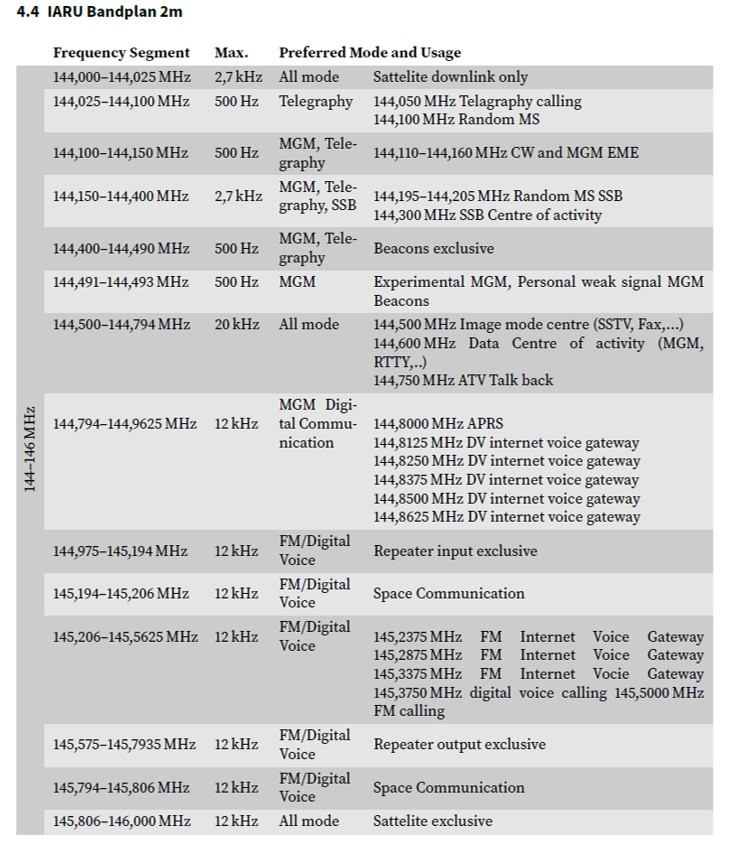
\includegraphics[width=0.85\textwidth]{foto/102}
    \caption{\scriptsize IARU-Bandplan \qty{2}{\metre}}
    \label{n_iaru_bandplan_2m}
\end{figure}

\end{frame}

\begin{frame}
\frametitle{Anruffrequenz}
Um schnell Funkpartner zu finden

\begin{itemize}
  \item FM-Sprechfunk (\enquote{FM calling})
  \item Digitale Telefonie (\enquote{digital voice calling})
  \end{itemize}

\end{frame}

\begin{frame}
\only<1>{
\begin{QQuestion}{BC205}{Welche Frequenz empfiehlt der IARU-Bandplan für einen allgemeinen Anruf mit analoger FM-Telefonie im \qty{2}{m}-Band?}{\qty{145,500}{\MHz}}
{\qty{144,050}{\MHz}}
{\qty{144,800}{\MHz}}
{\qty{145,800}{\MHz}}
\end{QQuestion}

}
\only<2>{
\begin{QQuestion}{BC205}{Welche Frequenz empfiehlt der IARU-Bandplan für einen allgemeinen Anruf mit analoger FM-Telefonie im \qty{2}{m}-Band?}{\textbf{\textcolor{DARCgreen}{\qty{145,500}{\MHz}}}}
{\qty{144,050}{\MHz}}
{\qty{144,800}{\MHz}}
{\qty{145,800}{\MHz}}
\end{QQuestion}

}
\end{frame}

\begin{frame}
\only<1>{
\begin{QQuestion}{BC207}{Welche Frequenz empfiehlt der IARU-Bandplan für einen allgemeinen Anruf mit digitaler Telefonie im \qty{2}{m}-Band?}{\qty{145,500}{\MHz}}
{\qty{145,375}{\MHz}}
{\qty{144,800}{\MHz}}
{\qty{144,195}{\MHz}}
\end{QQuestion}

}
\only<2>{
\begin{QQuestion}{BC207}{Welche Frequenz empfiehlt der IARU-Bandplan für einen allgemeinen Anruf mit digitaler Telefonie im \qty{2}{m}-Band?}{\qty{145,500}{\MHz}}
{\textbf{\textcolor{DARCgreen}{\qty{145,375}{\MHz}}}}
{\qty{144,800}{\MHz}}
{\qty{144,195}{\MHz}}
\end{QQuestion}

}
\end{frame}

\begin{frame}
\frametitle{Frequenzwechsel}
\begin{itemize}
  \item Anruffrequenzen für Anrufe freihalten
  \item Nach Verbindungsaufbau auf eine andere Frequenz verständigen
  \item Nützliche Frequenz aus dem Bandplan entnehmen
  \item Frequenz wechseln
  \end{itemize}
\end{frame}

\begin{frame}
\only<1>{
\begin{QQuestion}{BC209}{Auf welcher der folgenden Frequenzen könnten Sie beispielsweise unter Berücksichtigung des IARU-Bandplans im \qty{2}{\m}-Band eine FM-Telefonieverbindung durchführen?}{\qty{145,450}{\MHz}}
{\qty{144,250}{\MHz}}
{\qty{144,090}{\MHz}}
{\qty{144,450}{\MHz}}
\end{QQuestion}

}
\only<2>{
\begin{QQuestion}{BC209}{Auf welcher der folgenden Frequenzen könnten Sie beispielsweise unter Berücksichtigung des IARU-Bandplans im \qty{2}{\m}-Band eine FM-Telefonieverbindung durchführen?}{\textbf{\textcolor{DARCgreen}{\qty{145,450}{\MHz}}}}
{\qty{144,250}{\MHz}}
{\qty{144,090}{\MHz}}
{\qty{144,450}{\MHz}}
\end{QQuestion}

}
\end{frame}

\begin{frame}
\frametitle{Analoge SSB-Telefonie}
\begin{itemize}
  \item Es gibt keine Anruffrequenz
  \item Stattdessen ein \emph{Aktivitätszentrum} bzw. \emph{center of activity}
  \item Anrufe sollen im Umfeld dieser Frequenz stattfinden
  \item Es kann aber der ganze \enquote{SSB}-Bereich genutzt werden
  \end{itemize}
\end{frame}

\begin{frame}
\only<1>{
\begin{QQuestion}{BC211}{Welche Frequenz bzw. welchen Frequenzbereich sieht der IARU-Bandplan als Aktivitätszentrum für SSB-Telefonie im \qty{2}{m}-Band vor?}{\qty{145,500}{\MHz}}
{\qty{144,300}{\MHz}}
{\qtyrange{144,195}{144,205}{\MHz}}
{\qtyrange{144,110}{144,160}{\MHz}}
\end{QQuestion}

}
\only<2>{
\begin{QQuestion}{BC211}{Welche Frequenz bzw. welchen Frequenzbereich sieht der IARU-Bandplan als Aktivitätszentrum für SSB-Telefonie im \qty{2}{m}-Band vor?}{\qty{145,500}{\MHz}}
{\textbf{\textcolor{DARCgreen}{\qty{144,300}{\MHz}}}}
{\qtyrange{144,195}{144,205}{\MHz}}
{\qtyrange{144,110}{144,160}{\MHz}}
\end{QQuestion}

}
\end{frame}

\begin{frame}
\only<1>{
\begin{QQuestion}{BC210}{Auf welcher der folgenden Frequenzen könnten Sie unter Berücksichtigung des IARU-Bandplans im \qty{2}{m}-Band eine SSB-Telefonieverbindung beispielsweise durchführen?}{\qty{144,800}{\MHz}}
{\qty{145,450}{\MHz}}
{\qty{144,310}{\MHz}}
{\qty{144,450}{\MHz}}
\end{QQuestion}

}
\only<2>{
\begin{QQuestion}{BC210}{Auf welcher der folgenden Frequenzen könnten Sie unter Berücksichtigung des IARU-Bandplans im \qty{2}{m}-Band eine SSB-Telefonieverbindung beispielsweise durchführen?}{\qty{144,800}{\MHz}}
{\qty{145,450}{\MHz}}
{\textbf{\textcolor{DARCgreen}{\qty{144,310}{\MHz}}}}
{\qty{144,450}{\MHz}}
\end{QQuestion}

}
\end{frame}

\begin{frame}
\frametitle{Reservierte Frequenzbereiche}
\begin{itemize}
  \item Satelliten-Up- und Downlink (\enquote{satellite uplink}, \enquote{satellite downlink})
  \item Baken (\enquote{beacons})
  \item Relaisfunkstellen, Eingabe und Ausgabe (\enquote{repeater input}, \enquote{repeater output})
  \item Weltraumkommunikation (\enquote{space communication})
  \item Morsetelegrafie (\enquote{CW})
  \end{itemize}

\end{frame}

\begin{frame}
\only<1>{
\begin{QQuestion}{BC214}{Warum sollten Sie auf \qty{144,125}{\MHz} \underline{keine} Direktverbindung in FM-Telefonie zu einem Funkamateur aufnehmen, der sich im Nachbarort befindet? Der IARU-Bandplan empfiehlt diesen Bereich für die Nutzung durch~...}{Baken.}
{Repeater.}
{Weltraumkommunikation.}
{Morsetelegrafie und schmalbandige digitale Übertragungsverfahren.}
\end{QQuestion}

}
\only<2>{
\begin{QQuestion}{BC214}{Warum sollten Sie auf \qty{144,125}{\MHz} \underline{keine} Direktverbindung in FM-Telefonie zu einem Funkamateur aufnehmen, der sich im Nachbarort befindet? Der IARU-Bandplan empfiehlt diesen Bereich für die Nutzung durch~...}{Baken.}
{Repeater.}
{Weltraumkommunikation.}
{\textbf{\textcolor{DARCgreen}{Morsetelegrafie und schmalbandige digitale Übertragungsverfahren.}}}
\end{QQuestion}

}
\end{frame}

\begin{frame}
\only<1>{
\begin{QQuestion}{BC215}{Warum sollten Sie auf \qty{144,450}{\MHz} \underline{keine} Direktverbindung in FM-Telefonie zu einem Funkamateur aufnehmen, der sich im Nachbarort befindet? Der IARU-Bandplan sieht diesen Bereich exklusiv für die Nutzung durch~...}{Baken vor.}
{Repeater vor.}
{Weltraumkommunikation vor.}
{Morsetelegrafie und schmalbandige digitale Übertragungsverfahren vor.}
\end{QQuestion}

}
\only<2>{
\begin{QQuestion}{BC215}{Warum sollten Sie auf \qty{144,450}{\MHz} \underline{keine} Direktverbindung in FM-Telefonie zu einem Funkamateur aufnehmen, der sich im Nachbarort befindet? Der IARU-Bandplan sieht diesen Bereich exklusiv für die Nutzung durch~...}{\textbf{\textcolor{DARCgreen}{Baken vor.}}}
{Repeater vor.}
{Weltraumkommunikation vor.}
{Morsetelegrafie und schmalbandige digitale Übertragungsverfahren vor.}
\end{QQuestion}

}
\end{frame}

\begin{frame}
\only<1>{
\begin{QQuestion}{BC218}{Warum sollten Sie auf \qty{145,800}{\MHz} \underline{keine} Direktverbindung in FM-Telefonie zu einem Funkamateur aufnehmen, der sich im Nachbarort befindet? Der IARU-Bandplan empfiehlt diesen Bereich für die Nutzung durch ...}{Baken.}
{Repeater.}
{Morsetelegrafie und schmalbandige digitale Übertragungsverfahren.}
{Weltraumkommunikation.}
\end{QQuestion}

}
\only<2>{
\begin{QQuestion}{BC218}{Warum sollten Sie auf \qty{145,800}{\MHz} \underline{keine} Direktverbindung in FM-Telefonie zu einem Funkamateur aufnehmen, der sich im Nachbarort befindet? Der IARU-Bandplan empfiehlt diesen Bereich für die Nutzung durch ...}{Baken.}
{Repeater.}
{Morsetelegrafie und schmalbandige digitale Übertragungsverfahren.}
{\textbf{\textcolor{DARCgreen}{Weltraumkommunikation.}}}
\end{QQuestion}

}
\end{frame}

\begin{frame}
\only<1>{
\begin{QQuestion}{BC217}{Warum sollten Sie auf \qty{145,600}{\MHz} \underline{keine} Direktverbindung in FM-Telefonie zu einem Funkamateur aufnehmen, der sich im Nachbarort befindet? Der IARU-Bandplan empfiehlt diesen Bereich für die Nutzung durch ...}{Weltraumkommunikation.}
{Repeater.}
{Morsetelegrafie und schmalbandige digitale Übertragungsverfahren.}
{Baken.}
\end{QQuestion}

}
\only<2>{
\begin{QQuestion}{BC217}{Warum sollten Sie auf \qty{145,600}{\MHz} \underline{keine} Direktverbindung in FM-Telefonie zu einem Funkamateur aufnehmen, der sich im Nachbarort befindet? Der IARU-Bandplan empfiehlt diesen Bereich für die Nutzung durch ...}{Weltraumkommunikation.}
{\textbf{\textcolor{DARCgreen}{Repeater.}}}
{Morsetelegrafie und schmalbandige digitale Übertragungsverfahren.}
{Baken.}
\end{QQuestion}

}
\end{frame}

\begin{frame}
\only<1>{
\begin{QQuestion}{BC213}{Warum sollten Sie RTTY, PSK31 oder FT8 \underline{nicht} auf \qty{144,075}{MHz}  verwenden? Der IARU-Bandplan empfiehlt~...}{diesen Bereich bevorzugt für Morsetelegrafie zu nutzen.}
{in diesem Bereich maximal \qty{500}{\Hz} Bandbreite zu belegen, damit der Bereich besser genutzt werden kann.}
{den Einsatz von Computern für die Signalerzeugung zu vermeiden.}
{digitale Verfahren oberhalb von \qty{430}{\MHz} durchzuführen, da dort mehr Bandbreite zur Verfügung steht.}
\end{QQuestion}

}
\only<2>{
\begin{QQuestion}{BC213}{Warum sollten Sie RTTY, PSK31 oder FT8 \underline{nicht} auf \qty{144,075}{MHz}  verwenden? Der IARU-Bandplan empfiehlt~...}{\textbf{\textcolor{DARCgreen}{diesen Bereich bevorzugt für Morsetelegrafie zu nutzen.}}}
{in diesem Bereich maximal \qty{500}{\Hz} Bandbreite zu belegen, damit der Bereich besser genutzt werden kann.}
{den Einsatz von Computern für die Signalerzeugung zu vermeiden.}
{digitale Verfahren oberhalb von \qty{430}{\MHz} durchzuführen, da dort mehr Bandbreite zur Verfügung steht.}
\end{QQuestion}

}
\end{frame}%ENDCONTENT


\section{IARU-Bandplan für 70 cm}
\label{section:iaru_bandplan_70cm}
\begin{frame}%STARTCONTENT

\begin{figure}
    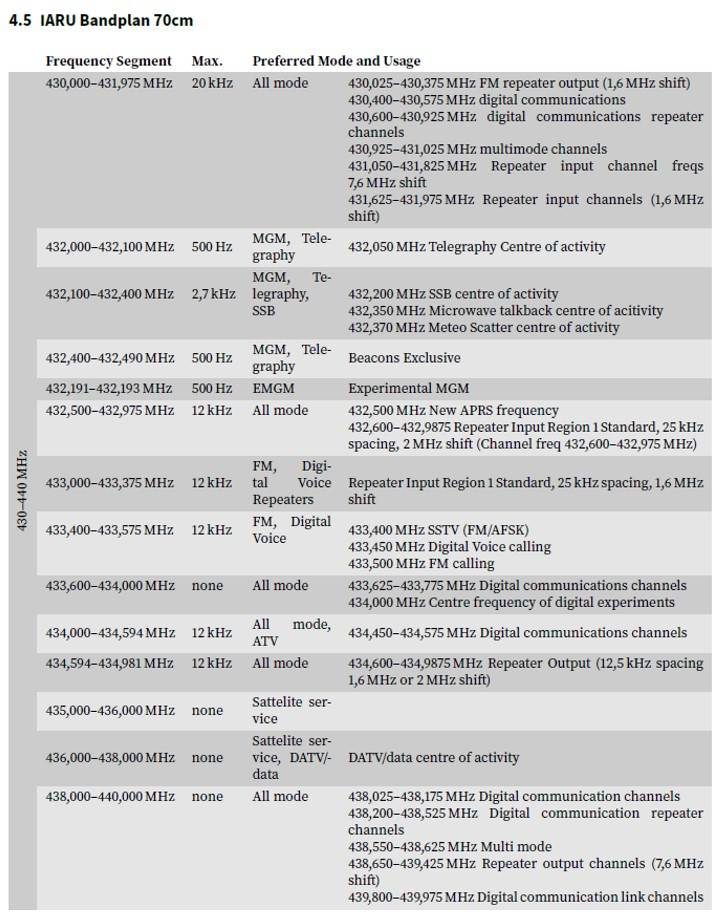
\includegraphics[width=0.85\textwidth]{foto/103}
    \caption{\scriptsize IARU-Bandplan \qty{70}{\centi\metre}}
    \label{n_iaru_bandplan_70cm}
\end{figure}

\end{frame}

\begin{frame}
\only<1>{
\begin{QQuestion}{BC206}{Welche Frequenz empfiehlt der IARU-Bandplan für einen allgemeinen Anruf mit analoger FM-Telefonie im \qty{70}{cm}-Band?}{\qty{433,450}{\MHz}}
{\qty{433,500}{\MHz}}
{\qty{432,500}{\MHz}}
{\qty{432,050}{\MHz}}
\end{QQuestion}

}
\only<2>{
\begin{QQuestion}{BC206}{Welche Frequenz empfiehlt der IARU-Bandplan für einen allgemeinen Anruf mit analoger FM-Telefonie im \qty{70}{cm}-Band?}{\qty{433,450}{\MHz}}
{\textbf{\textcolor{DARCgreen}{\qty{433,500}{\MHz}}}}
{\qty{432,500}{\MHz}}
{\qty{432,050}{\MHz}}
\end{QQuestion}

}
\end{frame}

\begin{frame}
\only<1>{
\begin{QQuestion}{BC208}{Welche Frequenz empfiehlt der IARU-Bandplan für einen allgemeinen Anruf mit digitaler Telefonie im \qty{70}{cm}-Band?}{\qty{433,500}{\MHz}}
{\qty{433,450}{\MHz}}
{\qty{432,500}{\MHz}}
{\qty{432,050}{\MHz}}
\end{QQuestion}

}
\only<2>{
\begin{QQuestion}{BC208}{Welche Frequenz empfiehlt der IARU-Bandplan für einen allgemeinen Anruf mit digitaler Telefonie im \qty{70}{cm}-Band?}{\qty{433,500}{\MHz}}
{\textbf{\textcolor{DARCgreen}{\qty{433,450}{\MHz}}}}
{\qty{432,500}{\MHz}}
{\qty{432,050}{\MHz}}
\end{QQuestion}

}
\end{frame}

\begin{frame}
\only<1>{
\begin{QQuestion}{BC212}{Welche Frequenz bzw. welchen Frequenzbereich sieht der IARU-Bandplan als Aktivitätszentrum für SSB-Telefonie im \qty{70}{cm}-Band vor?}{\qty{434,000}{\MHz}}
{\qty{432,200}{\MHz}}
{\qtyrange{432,600}{432,9875}{\MHz}}
{\qtyrange{434,450}{434,575}{\MHz}}
\end{QQuestion}

}
\only<2>{
\begin{QQuestion}{BC212}{Welche Frequenz bzw. welchen Frequenzbereich sieht der IARU-Bandplan als Aktivitätszentrum für SSB-Telefonie im \qty{70}{cm}-Band vor?}{\qty{434,000}{\MHz}}
{\textbf{\textcolor{DARCgreen}{\qty{432,200}{\MHz}}}}
{\qtyrange{432,600}{432,9875}{\MHz}}
{\qtyrange{434,450}{434,575}{\MHz}}
\end{QQuestion}

}
\end{frame}

\begin{frame}
\only<1>{
\begin{QQuestion}{BC221}{Warum sollten Sie auf \qty{435,500}{\MHz} \underline{keine} Direktverbindung in FM-Telefonie zu einem Funkamateur aufnehmen, der sich im Nachbarort befindet? Der IARU-Bandplan empfiehlt diesen Bereich für die Nutzung durch~...}{Satellitenfunk.}
{Repeater.}
{Morsetelegrafie und schmalbandige digitale Übertragungsverfahren.}
{Baken.}
\end{QQuestion}

}
\only<2>{
\begin{QQuestion}{BC221}{Warum sollten Sie auf \qty{435,500}{\MHz} \underline{keine} Direktverbindung in FM-Telefonie zu einem Funkamateur aufnehmen, der sich im Nachbarort befindet? Der IARU-Bandplan empfiehlt diesen Bereich für die Nutzung durch~...}{\textbf{\textcolor{DARCgreen}{Satellitenfunk.}}}
{Repeater.}
{Morsetelegrafie und schmalbandige digitale Übertragungsverfahren.}
{Baken.}
\end{QQuestion}

}
\end{frame}

\begin{frame}
\only<1>{
\begin{QQuestion}{BC222}{Warum sollten Sie auf \qty{439,200}{\MHz} \underline{keine} Direktverbindung in FM-Telefonie zu einem Funkamateur aufnehmen, der sich im Nachbarort befindet? Der IARU-Bandplan empfiehlt diesen Bereich für die Nutzung durch~...}{Morsetelegrafie und schmalbandige digitale Übertragungsverfahren.}
{Satellitenfunk.}
{Repeater.}
{Baken.}
\end{QQuestion}

}
\only<2>{
\begin{QQuestion}{BC222}{Warum sollten Sie auf \qty{439,200}{\MHz} \underline{keine} Direktverbindung in FM-Telefonie zu einem Funkamateur aufnehmen, der sich im Nachbarort befindet? Der IARU-Bandplan empfiehlt diesen Bereich für die Nutzung durch~...}{Morsetelegrafie und schmalbandige digitale Übertragungsverfahren.}
{Satellitenfunk.}
{\textbf{\textcolor{DARCgreen}{Repeater.}}}
{Baken.}
\end{QQuestion}

}
\end{frame}

\begin{frame}
\only<1>{
\begin{QQuestion}{BC219}{Warum sollten Sie auf \qty{432,040}{\MHz} \underline{keine} Direktverbindung in FM-Telefonie zu einem Funkamateur aufnehmen, der sich im Nachbarort befindet? Der IARU-Bandplan empfiehlt diesen Bereich für die Nutzung durch~...}{Weltraumkommunikation.}
{Satellitenfunk.}
{Morsetelegrafie und schmalbandige digitale Übertragungsverfahren.}
{Baken.}
\end{QQuestion}

}
\only<2>{
\begin{QQuestion}{BC219}{Warum sollten Sie auf \qty{432,040}{\MHz} \underline{keine} Direktverbindung in FM-Telefonie zu einem Funkamateur aufnehmen, der sich im Nachbarort befindet? Der IARU-Bandplan empfiehlt diesen Bereich für die Nutzung durch~...}{Weltraumkommunikation.}
{Satellitenfunk.}
{\textbf{\textcolor{DARCgreen}{Morsetelegrafie und schmalbandige digitale Übertragungsverfahren.}}}
{Baken.}
\end{QQuestion}

}
\end{frame}

\begin{frame}
\only<1>{
\begin{QQuestion}{BC220}{Warum sollten Sie auf \qty{432,450}{\MHz} \underline{keine} Direktverbindung in FM-Telefonie zu einem Funkamateur aufnehmen, der sich im Nachbarort befindet? Der IARU-Bandplan empfiehlt diesen Bereich exklusiv für die Nutzung durch~...}{Satellitenfunk.}
{Baken.}
{Repeater.}
{Morsetelegrafie und schmalbandige digitale Übertragungsverfahren.}
\end{QQuestion}

}
\only<2>{
\begin{QQuestion}{BC220}{Warum sollten Sie auf \qty{432,450}{\MHz} \underline{keine} Direktverbindung in FM-Telefonie zu einem Funkamateur aufnehmen, der sich im Nachbarort befindet? Der IARU-Bandplan empfiehlt diesen Bereich exklusiv für die Nutzung durch~...}{Satellitenfunk.}
{\textbf{\textcolor{DARCgreen}{Baken.}}}
{Repeater.}
{Morsetelegrafie und schmalbandige digitale Übertragungsverfahren.}
\end{QQuestion}

}
\end{frame}%ENDCONTENT


\section{Wellenausbreitung}
\label{section:wellenausbreitung}
\begin{frame}%STARTCONTENT

\begin{columns}
    \begin{column}{0.48\textwidth}
    Je nach Frequenz breitet sich eine Funkwelle anders über unseren Planeten aus.


\begin{figure}
    \DARCimage{0.85\linewidth}{731include}
    \caption{\scriptsize Ionosphäre, Troposhäre und Sporadic-E}
    \label{n_ionosphäre}
\end{figure}


    \end{column}
   \begin{column}{0.48\textwidth}
       \begin{itemize}
  \item Der Funkhorizont, der etwas weiter geht als der sichtbare Horizont (VHF, UHF und höher)
  \item Überreichweiten durch Wetterereignisse in der Troposphäre (VHF, UHF und höher)
  \item Besondere Überreichweiten durch Sporadic-E (VHF, UHF)
  \item Die Raumwelle durch Brechung an der Ionosphäre (Kurzwelle)
  \end{itemize}

   \end{column}
\end{columns}

\end{frame}%ENDCONTENT


\section{Funkhorizont}
\label{section:funkhorizont}
\begin{frame}%STARTCONTENT

\begin{columns}
    \begin{column}{0.48\textwidth}
    
\begin{figure}
    \DARCimage{0.85\linewidth}{484include}
    \caption{\scriptsize Ausbreitung}
    \label{n_funkhorizont}
\end{figure}


    \end{column}
   \begin{column}{0.48\textwidth}
       \begin{itemize}
  \item Funkwellen im VHF- und UHF-Bereich verhalten sich ähnlich wie Licht
  \item Licht reicht maximal bis zum geografischen (sichtbaren) Horizont
  \item Funkwellen schaffen ca. \qty{15}{\percent} mehr Reichweite
  \item Folgen ein wenig der Erdkrümmung
  \end{itemize}

   \end{column}
\end{columns}

\end{frame}

\begin{frame}\begin{itemize}
  \item Sichtverbindung für zuverlässige Funkverbindungen auf VHF, UHF und darüber
  \item Hohe Gebäude oder Berge stören
  \item Je höher die Antenne, umso größer die Reichweite
  \item Weite Verbindungen von Bergen statt aus dem Tal
  \end{itemize}
\end{frame}

\begin{frame}
\only<1>{
\begin{QQuestion}{NH301}{Wie weit etwa reicht der Funkhorizont im UKW-Bereich über den geografischen Horizont hinaus? Er reicht etwa~...}{doppelt so weit.}
{\qty{15}{\percent} weiter.}
{halb so weit.}
{bis zu viermal so weit.}
\end{QQuestion}

}
\only<2>{
\begin{QQuestion}{NH301}{Wie weit etwa reicht der Funkhorizont im UKW-Bereich über den geografischen Horizont hinaus? Er reicht etwa~...}{doppelt so weit.}
{\textbf{\textcolor{DARCgreen}{\qty{15}{\percent} weiter.}}}
{halb so weit.}
{bis zu viermal so weit.}
\end{QQuestion}

}
\end{frame}

\begin{frame}
\only<1>{
\begin{PQuestion}{NH303}{In dem folgenden Geländeprofil sei S ein Sender im \qty{2}{\m}-Band. Welche der Empfangsstationen E1 bis E4 wird das Signal des Senders wahrscheinlich am besten empfangen?}{$\text{E}_3$}
{$\text{E}_1$}
{$\text{E}_2$}
{$\text{E}_4$}
{\DARCimage{1.0\linewidth}{483include}}\end{PQuestion}

}
\only<2>{
\begin{PQuestion}{NH303}{In dem folgenden Geländeprofil sei S ein Sender im \qty{2}{\m}-Band. Welche der Empfangsstationen E1 bis E4 wird das Signal des Senders wahrscheinlich am besten empfangen?}{\textbf{\textcolor{DARCgreen}{$\text{E}_3$}}}
{$\text{E}_1$}
{$\text{E}_2$}
{$\text{E}_4$}
{\DARCimage{1.0\linewidth}{483include}}\end{PQuestion}

}
\end{frame}

\begin{frame}
\only<1>{
\begin{QQuestion}{NH302}{Wie wirkt sich die Antennenhöhe auf die Reichweite einer UKW-Verbindung aus? Die Reichweite steigt mit zunehmender Antennenhöhe, weil~...}{die quasi-optische Sichtweite zunimmt.}
{sie näher an der Ionosphäre ist.}
{dadurch steiler abgestrahlt werden kann.}
{in höheren Luftschichten die Temperatur sinkt.}
\end{QQuestion}

}
\only<2>{
\begin{QQuestion}{NH302}{Wie wirkt sich die Antennenhöhe auf die Reichweite einer UKW-Verbindung aus? Die Reichweite steigt mit zunehmender Antennenhöhe, weil~...}{\textbf{\textcolor{DARCgreen}{die quasi-optische Sichtweite zunimmt.}}}
{sie näher an der Ionosphäre ist.}
{dadurch steiler abgestrahlt werden kann.}
{in höheren Luftschichten die Temperatur sinkt.}
\end{QQuestion}

}
\end{frame}%ENDCONTENT


\section{Troposphärische Inversionsbildung}
\label{section:troposphaere}
\begin{frame}%STARTCONTENT

\begin{columns}
    \begin{column}{0.48\textwidth}
    
\begin{figure}
    \DARCimage{0.85\linewidth}{734include}
    \caption{\scriptsize Troposhärische Inversionsbildung, Schichten unterschiedlicher Temperatur liegen aufeinander, an der Grenze der Schichten werden Funkwellen im VHF-Bereich reflektiert}
    \label{n_tropo}
\end{figure}


    \end{column}
   \begin{column}{0.48\textwidth}
       \begin{itemize}
  \item Besonderer Effekt in der Troposphäre (ca. 15km)
  \item \emph{Troposphärische Inversionsschichten} zwischen warmen und kalten Luftschichten
  \item Führt zu erheblich größeren Reichweiten im VHF-Bereich (800-1000km)
  \item Tritt hauptsächlich im Frühjahr und Herbst auf
  \end{itemize}

   \end{column}
\end{columns}

\end{frame}

\begin{frame}
\only<1>{
\begin{QQuestion}{NH304}{Welcher Effekt ist normalerweise für die Ausbreitung eines VHF-Signals über 800~bis \qty{1 000}{\km} verantwortlich?}{Atmosphärische Absorption}
{Reflexion an der Mondoberfläche}
{Bodenwellenausbreitung}
{Troposphärische Inversionsbildung}
\end{QQuestion}

}
\only<2>{
\begin{QQuestion}{NH304}{Welcher Effekt ist normalerweise für die Ausbreitung eines VHF-Signals über 800~bis \qty{1 000}{\km} verantwortlich?}{Atmosphärische Absorption}
{Reflexion an der Mondoberfläche}
{Bodenwellenausbreitung}
{\textbf{\textcolor{DARCgreen}{Troposphärische Inversionsbildung}}}
\end{QQuestion}

}
\end{frame}%ENDCONTENT


\section{Sporadic-E}
\label{section:sporadic_e_1}
\begin{frame}%STARTCONTENT

\begin{columns}
    \begin{column}{0.48\textwidth}
    
\begin{figure}
    \DARCimage{0.85\linewidth}{733include}
    \caption{\scriptsize Refraktion (Brechung) von Funkwellen an stark ionisierten Bereichen der E-Schicht}
    \label{n_sporadic_e}
\end{figure}


    \end{column}
   \begin{column}{0.48\textwidth}
       \begin{itemize}
  \item Im Sommer mit größeren Reichweiten (1000-2000km)
  \item Refraktionen (Brechungen) an ionisierten Bereichen
  \item Treten in 100-110km in der E-Schicht auf
  \item Tritt zufällig und schwer vorhersagbar auf
  \item Sehr kleine Bereiche
  \end{itemize}

   \end{column}
\end{columns}

\end{frame}

\begin{frame}
\only<1>{
\begin{QQuestion}{NH306}{Ein Funkamateur sagt, dass auf dem \qty{2}{\m}-Band \glqq Sporadic-E-Bedingungen\grqq{} herrschen. Er meint damit, dass derzeit~...}{Stationen aus Entfernungen von \qtyrange{1000}{2000}{\km} zu hören sind, die über Reflexion an Ionisationserscheinungen des Polarkreises empfangen werden.}
{Stationen aus Nordamerika zu hören sind, die über Refraktion (Brechung) an energiereichen leuchtenden Nachtwolken (NLCs) empfangen werden.}
{Stationen aus Nordamerika zu hören sind, die über Reflexion an Ionisationserscheinungen des Polarkreises empfangen werden.}
{Stationen aus Entfernungen von \qtyrange{1000}{2000}{\km} zu hören sind, die über Refraktion (Brechung) in der sporadischen E-Region empfangen werden.}
\end{QQuestion}

}
\only<2>{
\begin{QQuestion}{NH306}{Ein Funkamateur sagt, dass auf dem \qty{2}{\m}-Band \glqq Sporadic-E-Bedingungen\grqq{} herrschen. Er meint damit, dass derzeit~...}{Stationen aus Entfernungen von \qtyrange{1000}{2000}{\km} zu hören sind, die über Reflexion an Ionisationserscheinungen des Polarkreises empfangen werden.}
{Stationen aus Nordamerika zu hören sind, die über Refraktion (Brechung) an energiereichen leuchtenden Nachtwolken (NLCs) empfangen werden.}
{Stationen aus Nordamerika zu hören sind, die über Reflexion an Ionisationserscheinungen des Polarkreises empfangen werden.}
{\textbf{\textcolor{DARCgreen}{Stationen aus Entfernungen von \qtyrange{1000}{2000}{\km} zu hören sind, die über Refraktion (Brechung) in der sporadischen E-Region empfangen werden.}}}
\end{QQuestion}

}
\end{frame}

\begin{frame}
\only<1>{
\begin{QQuestion}{NH305}{Bei welcher Ausbreitungsart wird über stark ionisierte Bereiche gearbeitet, die sich vor allem in den Sommermonaten in etwa 100 bis 110 Kilometer Höhe bilden?}{Troposphärische Ausbreitung}
{Sporadic-E}
{Reflexion an Inversionsschichten}
{Reflexion an Gewitterwolken}
\end{QQuestion}

}
\only<2>{
\begin{QQuestion}{NH305}{Bei welcher Ausbreitungsart wird über stark ionisierte Bereiche gearbeitet, die sich vor allem in den Sommermonaten in etwa 100 bis 110 Kilometer Höhe bilden?}{Troposphärische Ausbreitung}
{\textbf{\textcolor{DARCgreen}{Sporadic-E}}}
{Reflexion an Inversionsschichten}
{Reflexion an Gewitterwolken}
\end{QQuestion}

}
\end{frame}%ENDCONTENT


\section{Ionosphäre}
\label{section:ionosphaere}
\begin{frame}%STARTCONTENT

\begin{columns}
    \begin{column}{0.48\textwidth}
     
\begin{figure}
    \DARCimage{0.85\linewidth}{732include}
    \caption{\scriptsize Brechung an der Ionosphäre}
    \label{n_ionosphaere}
\end{figure}


    \end{column}
   \begin{column}{0.48\textwidth}
       \begin{itemize}
  \item Im oberen Teil der Erdatmosphäre
  \item Hat großen Einfluss im Kurzwellenbereich
  \item Sonnenstrahlung erzeugt elektrisch geladene Teilchen
  \item Funkwellen werden daran gebrochen (refraktiert) $\rightarrow$ Raumwelle
  \item Weltweite Funkverbindungen möglich
  \end{itemize}

   \end{column}
\end{columns}

\end{frame}

\begin{frame}
\only<1>{
\begin{QQuestion}{NH101}{Wie nennt sich der Bereich in der Atmosphäre, in dem die Kurzwellenausbreitung durch Brechung (Refraktion) ermöglicht wird?}{Hemisphäre}
{Magnetosphäre}
{Ionosphäre}
{Hydrosphäre}
\end{QQuestion}

}
\only<2>{
\begin{QQuestion}{NH101}{Wie nennt sich der Bereich in der Atmosphäre, in dem die Kurzwellenausbreitung durch Brechung (Refraktion) ermöglicht wird?}{Hemisphäre}
{Magnetosphäre}
{\textbf{\textcolor{DARCgreen}{Ionosphäre}}}
{Hydrosphäre}
\end{QQuestion}

}
\end{frame}

\begin{frame}
\only<1>{
\begin{QQuestion}{NH102}{Warum ist die Ionosphäre ausschlaggebend für die Kurzwellenausbreitung? In der Ionosphäre werden elektromagnetische Wellen durch~...}{Wärme verstärkt und reflektiert.}
{elektrisch geladene Teilchen gebrochen (refraktiert).}
{Kälte gebrochen und reflektiert.}
{Temperaturübergänge gebrochen (refraktiert).}
\end{QQuestion}

}
\only<2>{
\begin{QQuestion}{NH102}{Warum ist die Ionosphäre ausschlaggebend für die Kurzwellenausbreitung? In der Ionosphäre werden elektromagnetische Wellen durch~...}{Wärme verstärkt und reflektiert.}
{\textbf{\textcolor{DARCgreen}{elektrisch geladene Teilchen gebrochen (refraktiert).}}}
{Kälte gebrochen und reflektiert.}
{Temperaturübergänge gebrochen (refraktiert).}
\end{QQuestion}

}
\end{frame}

\begin{frame}
\begin{columns}
    \begin{column}{0.48\textwidth}
    
\begin{figure}
    \DARCimage{0.85\linewidth}{729include}
    \caption{\scriptsize Die Anzahl der Sonnenflecken, die über den elfjährige Sonnenzyklus schwankt}
    \label{n_ionosphaere_sonnenflecken}
\end{figure}


    \end{column}
   \begin{column}{0.48\textwidth}
       \begin{itemize}
  \item Ausbreitungsbedingungen wechseln täglich und nach Jahreszeit
  \item Sonnenflecken haben einen großen Einfluss
  \item Alle 11 Jahre treten starke Sonnenflecken auf
  \item Mehr elektromagnetische Strahlung und Materie in der Ionosphäre
  \end{itemize}

   \end{column}
\end{columns}

\end{frame}

\begin{frame}
\only<1>{
\begin{QQuestion}{NH201}{Was ist ein wesentlicher Faktor für die Ausbreitung von Kurzwellen über die Ionosphäre?}{Die Bandbreite der Antenne}
{Die Filterfunktion des Empfängers}
{Der elfjährige Sonnenzyklus}
{Die präzise Antennenausrichtung zum Äquator}
\end{QQuestion}

}
\only<2>{
\begin{QQuestion}{NH201}{Was ist ein wesentlicher Faktor für die Ausbreitung von Kurzwellen über die Ionosphäre?}{Die Bandbreite der Antenne}
{Die Filterfunktion des Empfängers}
{\textbf{\textcolor{DARCgreen}{Der elfjährige Sonnenzyklus}}}
{Die präzise Antennenausrichtung zum Äquator}
\end{QQuestion}

}
\end{frame}

\begin{frame}
\begin{columns}
    \begin{column}{0.48\textwidth}
    
\begin{figure}
    \DARCimage{0.85\linewidth}{741include}
    \caption{\scriptsize Die Tote Zone, die für die Bodenwelle zu nah und für die Raumwelle zu weit weg ist.}
    \label{n_ionosphaere_tote_zone}
\end{figure}


    \end{column}
   \begin{column}{0.48\textwidth}
       \begin{itemize}
  \item Auf Kurzwelle kann es zu einer \emph{Toten Zone} kommen
  \item Für die Bodenwelle zu weit -- für die Raumwelle zu nah
  \item Nur eine Seite einer Funkverbindung hörbar
  \end{itemize}

   \end{column}
\end{columns}

\end{frame}

\begin{frame}
\only<1>{
\begin{QQuestion}{BE106}{Eine Frequenz auf einem höheren Kurzwellenband erscheint zunächst frei, stellt sich aber anschließend als besetzt heraus. Was ist die häufigste Ursache dafür?}{Die auf dieser Frequenz sendende Station wurde durch den Mögel-Dellinger-Effekt kurzfristig unterbrochen.}
{Eine Station auf dieser Frequenz verwendet das andere Seitenband.}
{Für die auf dieser Frequenz sendenden Stationen sind die Ausbreitungsbedingungen zu schlecht.}
{Eine auf dieser Frequenz sendende Station liegt innerhalb der toten Zone und konnte daher von mir nicht gehört werden.}
\end{QQuestion}

}
\only<2>{
\begin{QQuestion}{BE106}{Eine Frequenz auf einem höheren Kurzwellenband erscheint zunächst frei, stellt sich aber anschließend als besetzt heraus. Was ist die häufigste Ursache dafür?}{Die auf dieser Frequenz sendende Station wurde durch den Mögel-Dellinger-Effekt kurzfristig unterbrochen.}
{Eine Station auf dieser Frequenz verwendet das andere Seitenband.}
{Für die auf dieser Frequenz sendenden Stationen sind die Ausbreitungsbedingungen zu schlecht.}
{\textbf{\textcolor{DARCgreen}{Eine auf dieser Frequenz sendende Station liegt innerhalb der toten Zone und konnte daher von mir nicht gehört werden.}}}
\end{QQuestion}

}
\end{frame}%ENDCONTENT


\title{DARC Amateurfunklehrgang Klasse N}
\author{Amateurfunkstationen}
\institute{Deutscher Amateur Radio Club e.\,V.}
\begin{frame}
\maketitle
\end{frame}

\section{Aufbau von Rufzeichen}
\label{section:rufzeichenaufbau}
\begin{frame}%STARTCONTENT

\frametitle{Personengebundene Rufzeichen}
\begin{itemize}
  \item Jeder Funkamateur mit Zulassung zum Amateurfunkdienst in Deutschland
  \item Rufzeichen wird durch die BNetzA zugeteilt
  \item Weltweit eindeutig
  \item Darf nur durch den zugeteilten Funkamateur benutzt werden
  \end{itemize}
\end{frame}

\begin{frame}
\only<1>{
\begin{QQuestion}{VC116}{Welche personengebundenen Rufzeichen darf ein Funkamateur benutzen?}{Bei Nutzung einer fremden Station das personengebundene Rufzeichen des Stationsinhabers}
{Beliebige Rufzeichen}
{Nur ein von einer Amateurfunkvereinigung zugeteiltes Rufzeichen}
{Nur ein ihm von der Bundesnetzagentur zugeteiltes Rufzeichen}
\end{QQuestion}

}
\only<2>{
\begin{QQuestion}{VC116}{Welche personengebundenen Rufzeichen darf ein Funkamateur benutzen?}{Bei Nutzung einer fremden Station das personengebundene Rufzeichen des Stationsinhabers}
{Beliebige Rufzeichen}
{Nur ein von einer Amateurfunkvereinigung zugeteiltes Rufzeichen}
{\textbf{\textcolor{DARCgreen}{Nur ein ihm von der Bundesnetzagentur zugeteiltes Rufzeichen}}}
\end{QQuestion}

}
\end{frame}

\begin{frame}
\frametitle{Aufbau von Rufzeichen}
\begin{columns}
    \begin{column}{0.48\textwidth}
    
\begin{figure}
    \DARCimage{0.85\linewidth}{654include}
    \caption{\scriptsize Aufbau Rufzeichen}
    \label{n_amateurfunkstrationen_aufbau_rufzeichen}
\end{figure}


    \end{column}
   \begin{column}{0.48\textwidth}
       Drei Teile:

\begin{itemize}
  \item Präfix
  \item Ziffer
  \item Suffix
  \end{itemize}

   \end{column}
\end{columns}

\end{frame}

\begin{frame}
\frametitle{Präfix}
\begin{itemize}
  \item Ist länderspezifisch zugeordnet
  \item Zur Lokalisierung von Amateurfunkstationen
  \item Werden durch die Internatione Fernmeldeunion (International Telecommunication Union, ITU) festgelegt
  \item Stehen in den Radio Regulations (RR)
  \item Mitgliedsstaaten sollen dieses in nationales Recht umsetzen
  \end{itemize}
\end{frame}

\begin{frame}
\frametitle{Präfixe Deutschland}
\begin{itemize}
  \item DA bis DR
  \item Y2 bis Y9
  \end{itemize}

\end{frame}

\begin{frame}
\only<1>{
\begin{QQuestion}{VA406}{Wo sind die Präfixe für Amateurfunkrufzeichen international geregelt?}{Im Amateurfunkgesetz (AFuG)}
{In den Radio Regulations (RR)}
{In der Rufzeichenliste der BNetzA}
{In der Amateurfunkverordnung (AFuV)}
\end{QQuestion}

}
\only<2>{
\begin{QQuestion}{VA406}{Wo sind die Präfixe für Amateurfunkrufzeichen international geregelt?}{Im Amateurfunkgesetz (AFuG)}
{\textbf{\textcolor{DARCgreen}{In den Radio Regulations (RR)}}}
{In der Rufzeichenliste der BNetzA}
{In der Amateurfunkverordnung (AFuV)}
\end{QQuestion}

}
\end{frame}

\begin{frame}
\frametitle{Personengebundene Rufzeichen Deutschland}
\begin{columns}
    \begin{column}{0.48\textwidth}
    \begin{itemize}
  \item 2 Buchstaben Präfix
  \item eine Ziffer
  \item 2-3 Buchstaben Suffix
  \end{itemize}

    \end{column}
   \begin{column}{0.48\textwidth}
       \begin{table}
\begin{DARCtabular}{l}
     DL1ABC   \\
     DO5XYZ   \\
     DA0RC   \\
\end{DARCtabular}
\caption{Beispiel für personengebundene, deutsche Amateurfunkrufzeichen}
\label{n_amateurfunkstationen_rufzeichen_beispiele}
\end{table}

   \end{column}
\end{columns}

\end{frame}

\begin{frame}
\only<1>{
\begin{QQuestion}{VD203}{Wie werden personengebundene deutsche Amateurfunkrufzeichen gebildet? Sie bestehen aus~...}{einem 2-buchstabigen Suffix (Landeskenner), zwei Ziffern und einem 2- oder 3-buchstabigen Präfix.}
{einem 2-buchstabigen Präfix (Landeskenner), einer Ziffer und einem 2- oder 3-buchstabigen Suffix.}
{einem 1-buchstabigen Präfix (Landeskenner), einer oder zwei Ziffern und einem 1-, 2- oder 3-buchstabigen Suffix.}
{einem 2-buchstabigen Suffix (Landeskenner), einer Ziffer und einem 1-, 2- oder 3-buchstabigen Präfix.}
\end{QQuestion}

}
\only<2>{
\begin{QQuestion}{VD203}{Wie werden personengebundene deutsche Amateurfunkrufzeichen gebildet? Sie bestehen aus~...}{einem 2-buchstabigen Suffix (Landeskenner), zwei Ziffern und einem 2- oder 3-buchstabigen Präfix.}
{\textbf{\textcolor{DARCgreen}{einem 2-buchstabigen Präfix (Landeskenner), einer Ziffer und einem 2- oder 3-buchstabigen Suffix.}}}
{einem 1-buchstabigen Präfix (Landeskenner), einer oder zwei Ziffern und einem 1-, 2- oder 3-buchstabigen Suffix.}
{einem 2-buchstabigen Suffix (Landeskenner), einer Ziffer und einem 1-, 2- oder 3-buchstabigen Präfix.}
\end{QQuestion}

}
\end{frame}

\begin{frame}
\frametitle{Weitere Rufzeichen}
\begin{itemize}
  \item Fernbediente und automatisch arbeitende Amateurfunkstellen
  \item Klubstationen
  \end{itemize}
\end{frame}

\begin{frame}
\only<1>{
\begin{QQuestion}{VD202}{Welche Rufzeichenzuteilungsarten gibt es im Amateurfunk unter anderem?}{Personengebundene Rufzeichen, Klubstationsrufzeichen, Contestrufzeichen}
{Personengebundene Rufzeichen, Familienrufzeichen, Klubstationsrufzeichen}
{Personengebundene Rufzeichen, Rufzeichen für fernbediente und automatisch arbeitende Amateurfunkstellen, Klubstationsrufzeichen}
{Personengebundene Rufzeichen, Rufzeichen für fernbediente und automatisch arbeitende Amateurfunkstellen, Mobilfunkrufzeichen}
\end{QQuestion}

}
\only<2>{
\begin{QQuestion}{VD202}{Welche Rufzeichenzuteilungsarten gibt es im Amateurfunk unter anderem?}{Personengebundene Rufzeichen, Klubstationsrufzeichen, Contestrufzeichen}
{Personengebundene Rufzeichen, Familienrufzeichen, Klubstationsrufzeichen}
{\textbf{\textcolor{DARCgreen}{Personengebundene Rufzeichen, Rufzeichen für fernbediente und automatisch arbeitende Amateurfunkstellen, Klubstationsrufzeichen}}}
{Personengebundene Rufzeichen, Rufzeichen für fernbediente und automatisch arbeitende Amateurfunkstellen, Mobilfunkrufzeichen}
\end{QQuestion}

}
\end{frame}

\begin{frame}
\frametitle{Rufzeichenplan}
\begin{itemize}
  \item In Deutschland durch die BNetzA
  \item Nach Rufzeichenplan (\textcolor{DARCblue}{\faLink~\href{https://50ohm.de/rzp}{50ohm.de/rzp}})
  \item Verwendungszweck erkennbar anhand von Präfix, Ziffern und Suffix
  \item Steht während der Prüfung zur Verfügung
  \end{itemize}

\end{frame}

\begin{frame}
\only<1>{
\begin{QQuestion}{VD201}{In welchem Regelwerk sind die Vorgaben für die Bildung von Rufzeichen für den Amateurfunkdienst in Deutschland zu finden?}{Im Rufzeichenplan der Bundesnetzagentur (BNetzA)}
{Im Amateurfunkgesetz (AFuG)}
{Im Bundesgesetzblatt (BGBl)}
{In den Radio Regulations (RR) der ITU}
\end{QQuestion}

}
\only<2>{
\begin{QQuestion}{VD201}{In welchem Regelwerk sind die Vorgaben für die Bildung von Rufzeichen für den Amateurfunkdienst in Deutschland zu finden?}{\textbf{\textcolor{DARCgreen}{Im Rufzeichenplan der Bundesnetzagentur (BNetzA)}}}
{Im Amateurfunkgesetz (AFuG)}
{Im Bundesgesetzblatt (BGBl)}
{In den Radio Regulations (RR) der ITU}
\end{QQuestion}

}
\end{frame}%ENDCONTENT


\section{Persönliche Rufzeichen}
\label{section:persoenliche_rufzeichen}
\begin{frame}%STARTCONTENT
\begin{itemize}
  \item Am häufigsten vergeben
  \item In Deutschland gibt es drei Zulassungsklassen
  \end{itemize}
\begin{enumerate}
  \item[1] Klasse~N (Entry Level License)
  \item[2] Klasse~E (Novice)
  \item[3] Klasse~A (Advanced)
  \end{enumerate}
\begin{itemize}
  \item Die Klasse ist am Präfix und der Ziffer erkennbar
  \end{itemize}

\end{frame}

\begin{frame}
\begin{columns}
    \begin{column}{0.48\textwidth}
    \begin{table}
\begin{DARCtabular}{lX}
     Klasse  & Präfix und Ziffer   \\
     Klasse~N  & DN9   \\
     Klasse~E  & DO1 -- DO9   \\
     Klasse~A  & DB1 -- DD9   \\
      & DF1 -- DH9   \\
      & DJ1 -- DM9   \\
\end{DARCtabular}
\caption{Präfixe und Ziffern für personengebunde Rufzeichen}
\label{n_persoenliche_rufzeichen_praefixe}
\end{table}

    \end{column}
   \begin{column}{0.48\textwidth}
       \begin{table}
\begin{DARCtabular}{lX}
     Klasse  & Rufzeichen   \\
     Klasse~N  & DN9AAA, DN9BB   \\
     Klasse~E  & DO2AAA, DO2BB   \\
     Klasse~A  & DL3AAA, DL3BB   \\
\end{DARCtabular}
\caption{Beispiele für personengebunde Rufzeichen}
\label{n_persoenliche_rufzeichen_beispiele}
\end{table}

   \end{column}
\end{columns}

\end{frame}

\begin{frame}
\only<1>{
\begin{QQuestion}{BD105}{Zu welcher Rufzeichenart gehören Rufzeichen, die mit DN9 beginnen?}{Personengebundene Rufzeichen für Kurzwellenhörer}
{Personengebundene Rufzeichen der Klasse~A}
{Personengebundene Rufzeichen der Klasse~E}
{Personengebundene Rufzeichen der Klasse~N}
\end{QQuestion}

}
\only<2>{
\begin{QQuestion}{BD105}{Zu welcher Rufzeichenart gehören Rufzeichen, die mit DN9 beginnen?}{Personengebundene Rufzeichen für Kurzwellenhörer}
{Personengebundene Rufzeichen der Klasse~A}
{Personengebundene Rufzeichen der Klasse~E}
{\textbf{\textcolor{DARCgreen}{Personengebundene Rufzeichen der Klasse~N}}}
\end{QQuestion}

}
\end{frame}

\begin{frame}
\only<1>{
\begin{QQuestion}{BD106}{Zu welcher Rufzeichenart gehören Rufzeichen, die mit DO1 bis DO9 beginnen und ein zwei- oder dreistelliges Suffix haben? Personengebundene Rufzeichen der~...}{Klasse K}
{Klasse A}
{Klasse N}
{Klasse E}
\end{QQuestion}

}
\only<2>{
\begin{QQuestion}{BD106}{Zu welcher Rufzeichenart gehören Rufzeichen, die mit DO1 bis DO9 beginnen und ein zwei- oder dreistelliges Suffix haben? Personengebundene Rufzeichen der~...}{Klasse K}
{Klasse A}
{Klasse N}
{\textbf{\textcolor{DARCgreen}{Klasse E}}}
\end{QQuestion}

}
\end{frame}

\begin{frame}
\only<1>{
\begin{QQuestion}{BD104}{Zu welcher Rufzeichenart gehören Rufzeichen, die mit DL1 bis DL9 beginnen und ein zwei- oder dreistelliges Suffix haben? Personengebundene Rufzeichen der~...}{Klasse E}
{Klasse A}
{Klasse N}
{Klasse K}
\end{QQuestion}

}
\only<2>{
\begin{QQuestion}{BD104}{Zu welcher Rufzeichenart gehören Rufzeichen, die mit DL1 bis DL9 beginnen und ein zwei- oder dreistelliges Suffix haben? Personengebundene Rufzeichen der~...}{Klasse E}
{\textbf{\textcolor{DARCgreen}{Klasse A}}}
{Klasse N}
{Klasse K}
\end{QQuestion}

}
\end{frame}

\begin{frame}
\frametitle{Zulassung}
\begin{itemize}
  \item Nach bestandener Prüfung Antrag bei BNetzA stellen auf \emph{Zulassung zur Teilnahme am Amateurfunkdienst}
  \item Darauf kommt die Zulassungsurkunde mit persönlichem Rufzeichen
  \item Erst danach darf Funkbetrieb aufgenommen werden
  \item Die Zulassung ist nicht übertragbar
  \end{itemize}

\end{frame}

\begin{frame}
\only<1>{
\begin{QQuestion}{VC107}{Darf ein Funkamateur seine Amateurfunkzulassung vorübergehend einer anderen Person übertragen? Die Amateurfunkzulassung ist~...}{an die in der Zulassungsurkunde angegebene Person gebunden und nicht übertragbar.}
{nach vorheriger Anzeige bei der Bundesnetzagentur an Personen im gleichen Haushalt übertragbar.}
{übertragbar, wenn es sich bei der Person um einen Funkamateur mit erfolgreich abgelegter Prüfung handelt.}
{übertragbar, wenn es sich um ausländische Funkamateure handelt, die sich vorübergehend in Deutschland aufhalten.}
\end{QQuestion}

}
\only<2>{
\begin{QQuestion}{VC107}{Darf ein Funkamateur seine Amateurfunkzulassung vorübergehend einer anderen Person übertragen? Die Amateurfunkzulassung ist~...}{\textbf{\textcolor{DARCgreen}{an die in der Zulassungsurkunde angegebene Person gebunden und nicht übertragbar.}}}
{nach vorheriger Anzeige bei der Bundesnetzagentur an Personen im gleichen Haushalt übertragbar.}
{übertragbar, wenn es sich bei der Person um einen Funkamateur mit erfolgreich abgelegter Prüfung handelt.}
{übertragbar, wenn es sich um ausländische Funkamateure handelt, die sich vorübergehend in Deutschland aufhalten.}
\end{QQuestion}

}
\end{frame}

\begin{frame}
\frametitle{Wunschrufzeichen}
\begin{itemize}
  \item Auf dem Antrag können Wunschrufzeichen angegeben werden
  \item In der Rufzeichenliste der BNetzA (\textcolor{DARCblue}{\faLink~\href{https://50ohm.de/rzl}{50ohm.de/rzl}}) oder in der Webabfrage der BNetzA (\textcolor{DARCblue}{\faLink~\href{https://50ohm.de/rza}{50ohm.de/rza}}) nach freien Rufzeichen schauen
  \item Es gibt keinen Anspruch auf die Zuteilung eines bestimmten Rufzeichens
  \item Ohne Wunschrufzeichen wählt die BNetzA ein Rufzeichen aus
  \end{itemize}

\end{frame}

\begin{frame}
\frametitle{Auswahl von Rufzeichen}
\begin{itemize}
  \item Kurzschreibweise des Namens
  \item Initialen
  \item Gute Verständlichkeit beim Sprechen
  \item Einfache Morsetelegrafie
  \item Wortwitz
  \end{itemize}
\end{frame}

\begin{frame}
\only<1>{
\begin{QQuestion}{VD208}{Hat ein Funkamateur Anspruch auf Zuteilung eines bestimmten Rufzeichens?}{Ja, wenn es noch nicht vergeben ist.}
{Nein, es besteht kein Anspruch darauf.}
{Nein, es sei denn, er kann besondere persönliche Gründe geltend machen und das Rufzeichen ist frei.}
{Ja, wenn es ihm schon einmal zugeteilt war.}
\end{QQuestion}

}
\only<2>{
\begin{QQuestion}{VD208}{Hat ein Funkamateur Anspruch auf Zuteilung eines bestimmten Rufzeichens?}{Ja, wenn es noch nicht vergeben ist.}
{\textbf{\textcolor{DARCgreen}{Nein, es besteht kein Anspruch darauf.}}}
{Nein, es sei denn, er kann besondere persönliche Gründe geltend machen und das Rufzeichen ist frei.}
{Ja, wenn es ihm schon einmal zugeteilt war.}
\end{QQuestion}

}
\end{frame}

\begin{frame}
\frametitle{Änderung von Rufzeichen}
\begin{itemize}
  \item In der Regel ändert die BNetzA ein Rufzeichen nicht
  \item Bei Änderungen von Regularien oder Zulassungsklassen kann es notwendig werden
  \item Bei Stellung eines neuen Antrags auf Zulassung zum Amateurfunkdienst wird ein neues Rufzeichen vergeben
  \end{itemize}

\end{frame}

\begin{frame}
\only<1>{
\begin{QQuestion}{VC117}{Kann ein zugeteiltes Rufzeichen durch die Bundesnetzagentur geändert werden?}{Das zugeteilte Rufzeichen ist Eigentum des Funkamateurs, das durch die Bundesnetzagentur nicht geändert wird.}
{Bei Umzug in den Zuständigkeitsbereich einer anderen Außenstelle der Bundesnetzagentur erhält der Funkamateur eine neue Rufzeichenzuteilung.}
{Aus wichtigen Gründen, insbesondere bei Änderungen internationaler Vorgaben, kann das Rufzeichen geändert werden.}
{Bei Änderung der Anzeige zur Verordnung über das Nachweisverfahren zur Begrenzung elektromagnetischer Felder (BEMFV) erhält der Funkamateur ein anderes Rufzeichen.}
\end{QQuestion}

}
\only<2>{
\begin{QQuestion}{VC117}{Kann ein zugeteiltes Rufzeichen durch die Bundesnetzagentur geändert werden?}{Das zugeteilte Rufzeichen ist Eigentum des Funkamateurs, das durch die Bundesnetzagentur nicht geändert wird.}
{Bei Umzug in den Zuständigkeitsbereich einer anderen Außenstelle der Bundesnetzagentur erhält der Funkamateur eine neue Rufzeichenzuteilung.}
{\textbf{\textcolor{DARCgreen}{Aus wichtigen Gründen, insbesondere bei Änderungen internationaler Vorgaben, kann das Rufzeichen geändert werden.}}}
{Bei Änderung der Anzeige zur Verordnung über das Nachweisverfahren zur Begrenzung elektromagnetischer Felder (BEMFV) erhält der Funkamateur ein anderes Rufzeichen.}
\end{QQuestion}

}
\end{frame}%ENDCONTENT


\section{Klubstationen}
\label{section:klubstationen}
\begin{frame}%STARTCONTENT

\begin{columns}
    \begin{column}{0.48\textwidth}
    
\begin{figure}
    \includegraphics[width=0.85\textwidth]{foto/58}
    \caption{\scriptsize Eine Klubstation}
    \label{n_klubstationen_klubstation}
\end{figure}

    \end{column}
   \begin{column}{0.48\textwidth}
       \begin{itemize}
  \item Gemeinsamer Betrieb einer Station
  \item Gruppe von mindestens 3 Funkamateuren
  \item Erhalten ein spezielles Rufzeichen
  \end{itemize}

   \end{column}
\end{columns}

\end{frame}

\begin{frame}
\only<1>{
\begin{QQuestion}{VD117}{Wie ist der Begriff \glqq Klubstation\grqq{} nach dem Wortlaut der Amateurfunkverordnung (AFuV) definiert?}{Eine \glqq Klubstation\grqq{} ist eine Amateurfunkstelle, die von mindestens drei Mitgliedern einer Gruppe von Funkamateuren unter Verwendung eines gemeinschaftlich genutzten Rufzeichens betrieben wird.}
{Eine \glqq Klubstation\grqq{} ist eine Amateurfunkstelle, die von mindestens vier Mitgliedern einer Gruppe von Funkamateuren unter Verwendung ihres personengebundenen Rufzeichens betrieben wird.}
{Eine \glqq Klubstation\grqq{} ist eine Amateurfunkstelle, die an einem geografisch exponierten Standort betrieben wird.}
{Eine \glqq Klubstation\grqq{} ist eine Amateurfunkstelle, die nur von einem eingetragenen Verein betrieben werden darf.}
\end{QQuestion}

}
\only<2>{
\begin{QQuestion}{VD117}{Wie ist der Begriff \glqq Klubstation\grqq{} nach dem Wortlaut der Amateurfunkverordnung (AFuV) definiert?}{\textbf{\textcolor{DARCgreen}{Eine \glqq Klubstation\grqq{} ist eine Amateurfunkstelle, die von mindestens drei Mitgliedern einer Gruppe von Funkamateuren unter Verwendung eines gemeinschaftlich genutzten Rufzeichens betrieben wird.}}}
{Eine \glqq Klubstation\grqq{} ist eine Amateurfunkstelle, die von mindestens vier Mitgliedern einer Gruppe von Funkamateuren unter Verwendung ihres personengebundenen Rufzeichens betrieben wird.}
{Eine \glqq Klubstation\grqq{} ist eine Amateurfunkstelle, die an einem geografisch exponierten Standort betrieben wird.}
{Eine \glqq Klubstation\grqq{} ist eine Amateurfunkstelle, die nur von einem eingetragenen Verein betrieben werden darf.}
\end{QQuestion}

}
\end{frame}

\begin{frame}
\frametitle{Rufzeichenplan}
\begin{columns}
    \begin{column}{0.48\textwidth}
    \begin{table}
\begin{DARCtabular}{llll}
     Rufzeichen  &  &  & Klasse   \\
     DAØAA  & --  & DAØZZZ  & A   \\
     DAØA  & --  & DA3Z  & A   \\
     DA6A  & --  & DA9Z  & E   \\
     DBØA  & --  & DD9Z  & A   \\
     DFØA  & --  & DH9Z  & A   \\
     DJØA  & --  & DM9Z  & A   \\
     DFØAA  & --  & DFØZZZ  & A   \\
\end{DARCtabular}
\caption{Rufzeichen für Klubstationen}
\label{n_klubstation_rufzeichen_1}
\end{table}

    \end{column}
   \begin{column}{0.48\textwidth}
       \begin{table}
\begin{DARCtabular}{llll}
     Rufzeichen  &  &  & Klasse   \\
     DKØAA  & --  & DKØZZZ  & A   \\
     DLØAA  & --  & DLØZZZ  & A   \\
     DNØA  & --  & DNØZ  & E   \\
     DNØAA  & --  & DNØZZZ  & E   \\
     DOØA  & --  & DO9Z  & E   \\
     DP3A  & --  & DP9Z  & A   \\
     DQØA  & --  & DR9Z  & A   \\
\end{DARCtabular}
\caption{Rufzeichen für Klubstationen}
\label{n_klubstation_rufzeichen_2}
\end{table}

   \end{column}
\end{columns}

\end{frame}

\begin{frame}
\only<1>{
\begin{QQuestion}{BD101}{Sie hören die Station DA0ABC. Um welche Art von Amateurfunkstelle handelt es sich? Es handelt sich um eine~...}{Amateurfunkstelle, die für besondere experimentelle Studien gemäß § 16 Absatz 2 AFuV betrieben wird.}
{Klubstation.}
{Amateurfunkstelle von Angehörigen der Gaststreitkräfte.}
{exterritoriale Station.}
\end{QQuestion}

}
\only<2>{
\begin{QQuestion}{BD101}{Sie hören die Station DA0ABC. Um welche Art von Amateurfunkstelle handelt es sich? Es handelt sich um eine~...}{Amateurfunkstelle, die für besondere experimentelle Studien gemäß § 16 Absatz 2 AFuV betrieben wird.}
{\textbf{\textcolor{DARCgreen}{Klubstation.}}}
{Amateurfunkstelle von Angehörigen der Gaststreitkräfte.}
{exterritoriale Station.}
\end{QQuestion}

}
\end{frame}

\begin{frame}
\only<1>{
\begin{QQuestion}{BD103}{Sie hören in einem Contest die Station DL0XK. Um welche Art von Amateurfunkstelle handelt es sich? Es handelt sich um eine Amateurfunkstelle~...}{mit personengebundenem Rufzeichen der Klasse E.}
{mit Klubstationsrufzeichen der Klasse E.}
{mit personengebundenem Rufzeichen der Klasse A.}
{mit Klubstationsrufzeichen der Klasse A.}
\end{QQuestion}

}
\only<2>{
\begin{QQuestion}{BD103}{Sie hören in einem Contest die Station DL0XK. Um welche Art von Amateurfunkstelle handelt es sich? Es handelt sich um eine Amateurfunkstelle~...}{mit personengebundenem Rufzeichen der Klasse E.}
{mit Klubstationsrufzeichen der Klasse E.}
{mit personengebundenem Rufzeichen der Klasse A.}
{\textbf{\textcolor{DARCgreen}{mit Klubstationsrufzeichen der Klasse A.}}}
\end{QQuestion}

}
\end{frame}

\begin{frame}
\frametitle{Stationsverantwortlicher}
\begin{itemize}
  \item Zur Beantragung ist ein Stationsverantwortlicher zu benennen
  \item Muss selbst Funkamateur mit Zulassung sein
  \item Rufzeichenklasse muss der für die Klubstation gleich sein
  \item Wird Inhaber eines auf 5 Jahre zugeteilten Rufzeichens
  \item Verlängerung muss rechtzeitig beantragt werden
  \item Verwendung erst nach Zuteilung möglich
  \end{itemize}
\end{frame}

\begin{frame}
\only<1>{
\begin{QQuestion}{VD401}{Welche Voraussetzungen müssen für die Erteilung eines Rufzeichens für den Betrieb einer Klubstation erfüllt sein?}{Der verantwortliche Funkamateur für die Klubstation muss in jedem Fall Inhaber eines Rufzeichens der höchsten Amateurfunkklasse sein.}
{Die Rufzeichenzuteilung für das Betreiben einer Klubstation ist von der Benennung des verantwortlichen Funkamateurs durch den Leiter einer Gruppe von Funkamateuren abhängig.}
{Der verantwortliche Funkamateur muss seit mindestens 2 Jahren Inhaber eines Amateurfunkzeugnisses sein.}
{Der Leiter einer als eingetragener Verein (e.\,V.) bestehenden Amateurfunkvereinigung muss auch der für die beantragte Klubstation verantwortliche Funkamateur sein.}
\end{QQuestion}

}
\only<2>{
\begin{QQuestion}{VD401}{Welche Voraussetzungen müssen für die Erteilung eines Rufzeichens für den Betrieb einer Klubstation erfüllt sein?}{Der verantwortliche Funkamateur für die Klubstation muss in jedem Fall Inhaber eines Rufzeichens der höchsten Amateurfunkklasse sein.}
{\textbf{\textcolor{DARCgreen}{Die Rufzeichenzuteilung für das Betreiben einer Klubstation ist von der Benennung des verantwortlichen Funkamateurs durch den Leiter einer Gruppe von Funkamateuren abhängig.}}}
{Der verantwortliche Funkamateur muss seit mindestens 2 Jahren Inhaber eines Amateurfunkzeugnisses sein.}
{Der Leiter einer als eingetragener Verein (e.\,V.) bestehenden Amateurfunkvereinigung muss auch der für die beantragte Klubstation verantwortliche Funkamateur sein.}
\end{QQuestion}

}
\end{frame}

\begin{frame}
\only<1>{
\begin{QQuestion}{VD402}{Welche Voraussetzung muss für die Erteilung eines Rufzeichens für den Betrieb einer Klubstation erfüllt sein?}{Eine Zulassung zur Teilnahme am Amateurfunkdienst nach \S~3 Abs. 1 AFuG.}
{Der verantwortliche Funkamateur für die Klubstation muss in jedem Fall Betreiber einer automatisch arbeitenden Station sein.}
{Der verantwortliche Funkamateur für die Klubstation muss in jedem Fall Inhaber eines Rufzeichens der höchsten Amateurfunkklasse sein.}
{Eine HAREC-Bescheinigung oder ein Amateurfunkzeugnis}
\end{QQuestion}

}
\only<2>{
\begin{QQuestion}{VD402}{Welche Voraussetzung muss für die Erteilung eines Rufzeichens für den Betrieb einer Klubstation erfüllt sein?}{\textbf{\textcolor{DARCgreen}{Eine Zulassung zur Teilnahme am Amateurfunkdienst nach \S~3 Abs. 1 AFuG.}}}
{Der verantwortliche Funkamateur für die Klubstation muss in jedem Fall Betreiber einer automatisch arbeitenden Station sein.}
{Der verantwortliche Funkamateur für die Klubstation muss in jedem Fall Inhaber eines Rufzeichens der höchsten Amateurfunkklasse sein.}
{Eine HAREC-Bescheinigung oder ein Amateurfunkzeugnis}
\end{QQuestion}

}
\end{frame}

\begin{frame}
\only<1>{
\begin{QQuestion}{VD403}{Ab wann darf ein Funkamateur laut Amateurfunkgesetz (AFuG) eine Klubstation betreiben?}{Nachdem er selbst eine Zulassung zum Amateurfunkdienst und die Zuteilung eines Klubstationsrufzeichens erhalten hat}
{Erst 3 Monate nach Ablegen der Amateurfunkprüfung und Zuteilung eines Klubstationsrufzeichens}
{Nach Vorlage einer harmonisierten Prüfungsbescheinigung kann der Betrieb erfolgen}
{Erst nach Überprüfung des Standortes durch die BNetzA und Zuteilung eines Klubstationsrufzeichens}
\end{QQuestion}

}
\only<2>{
\begin{QQuestion}{VD403}{Ab wann darf ein Funkamateur laut Amateurfunkgesetz (AFuG) eine Klubstation betreiben?}{\textbf{\textcolor{DARCgreen}{Nachdem er selbst eine Zulassung zum Amateurfunkdienst und die Zuteilung eines Klubstationsrufzeichens erhalten hat}}}
{Erst 3 Monate nach Ablegen der Amateurfunkprüfung und Zuteilung eines Klubstationsrufzeichens}
{Nach Vorlage einer harmonisierten Prüfungsbescheinigung kann der Betrieb erfolgen}
{Erst nach Überprüfung des Standortes durch die BNetzA und Zuteilung eines Klubstationsrufzeichens}
\end{QQuestion}

}
\end{frame}

\begin{frame}
\frametitle{Nutzung}
\begin{itemize}
  \item Von jedem Funkamateur mit Zulassung
  \item Nicht auf die Mitglieder der Gruppe beschränkt
  \end{itemize}
\end{frame}

\begin{frame}
\only<1>{
\begin{QQuestion}{VD404}{Was ist nötig, damit ein Funkamateur das Rufzeichen einer Klubstation mitbenutzen darf?}{Er muss Inhaber eines Rufzeichens der höchsten Amateurfunkklasse sein.}
{Er muss Mitglied in der Gruppe der Funkamateure sein, die die Klubstation betreibt.}
{Er muss im Besitz eines Amateurfunkzeugnisses sein, dass der Klasse der Klubstation entspricht.}
{Er muss Inhaber einer Zulassung zur Teilnahme am Amateurfunkdienst sein.}
\end{QQuestion}

}
\only<2>{
\begin{QQuestion}{VD404}{Was ist nötig, damit ein Funkamateur das Rufzeichen einer Klubstation mitbenutzen darf?}{Er muss Inhaber eines Rufzeichens der höchsten Amateurfunkklasse sein.}
{Er muss Mitglied in der Gruppe der Funkamateure sein, die die Klubstation betreibt.}
{Er muss im Besitz eines Amateurfunkzeugnisses sein, dass der Klasse der Klubstation entspricht.}
{\textbf{\textcolor{DARCgreen}{Er muss Inhaber einer Zulassung zur Teilnahme am Amateurfunkdienst sein.}}}
\end{QQuestion}

}
\end{frame}

\begin{frame}
\only<1>{
\begin{QQuestion}{VD405}{Darf ein Funkamateur mit Zulassung zur Teilnahme am Amateurfunkdienst nach den Bestimmungen der Amateurfunkverordnung (AFuV) mit dem Rufzeichen der Klubstation Funkbetrieb durchführen, auch wenn er nicht Mitglied der betreibenden Gruppe ist?}{Der Funkamateur muss dieses mindestens zwei Tage zuvor der BNetzA anzeigen.}
{Nur die Mitglieder der Gruppe dürfen die Klubstation betreiben.}
{Der Funkbetrieb muss im Beisein eines Gruppenmitglieds erfolgen.}
{An Klubstationen dürfen auch Nichtmitglieder Funkbetrieb durchführen.}
\end{QQuestion}

}
\only<2>{
\begin{QQuestion}{VD405}{Darf ein Funkamateur mit Zulassung zur Teilnahme am Amateurfunkdienst nach den Bestimmungen der Amateurfunkverordnung (AFuV) mit dem Rufzeichen der Klubstation Funkbetrieb durchführen, auch wenn er nicht Mitglied der betreibenden Gruppe ist?}{Der Funkamateur muss dieses mindestens zwei Tage zuvor der BNetzA anzeigen.}
{Nur die Mitglieder der Gruppe dürfen die Klubstation betreiben.}
{Der Funkbetrieb muss im Beisein eines Gruppenmitglieds erfolgen.}
{\textbf{\textcolor{DARCgreen}{An Klubstationen dürfen auch Nichtmitglieder Funkbetrieb durchführen.}}}
\end{QQuestion}

}
\end{frame}

\begin{frame}
\frametitle{Funkbetrieb}
\begin{itemize}
  \item Klasse~N oder E darf an Klubstation mit Klasse~A Betrieb machen
  \item $\rightarrow$ Jedoch nur im Rahmen seiner Bänder und Leistung
  \item Klasse~A darf an Klubstation der Klasse~E oder N Betrieb machen
  \item $\rightarrow$ Jedoch nur im Rahmen der Bänder und Leistung der Klubstation
  \end{itemize}
    \pause
    Die niedrigste Klasse gibt die maximale Berechtigung vor.



\end{frame}

\begin{frame}\begin{table}
\begin{DARCtabular}{lccc}
      & Station N  & Station E  & Station A   \\
     Funkamateur N  & N  & N  & N   \\
     Funkamateur E  & N  & E  & E   \\
     Funkamateur A  & N  & E  & A   \\
\end{DARCtabular}
\caption{Darstellung im Rahmen welcher Klasse Funkbetrieb durchgeführt werden darf, wenn sich Klasse des Funkamateurs und Klasse der Klubstation unterscheiden}
\label{n_klubstation_unterschiedliche_klassen}
\end{table}

\end{frame}

\begin{frame}
\only<1>{
\begin{QQuestion}{VD406}{Sie nutzen ein Klubstationsrufzeichen und verfügen über eine andere Amateurfunkzeugnis-Klasse als die Zuteilung der Klubstation. In welchen Frequenzbereichen und mit welchen Leistungen dürfen Sie senden? Entsprechend des Berechtigungsumfangs~...}{der niedrigeren der beiden Klassen.}
{der höheren der beiden Klassen.}
{der Klasse meiner persönlichen Zulassung.}
{der Klasse der Klubstation.}
\end{QQuestion}

}
\only<2>{
\begin{QQuestion}{VD406}{Sie nutzen ein Klubstationsrufzeichen und verfügen über eine andere Amateurfunkzeugnis-Klasse als die Zuteilung der Klubstation. In welchen Frequenzbereichen und mit welchen Leistungen dürfen Sie senden? Entsprechend des Berechtigungsumfangs~...}{\textbf{\textcolor{DARCgreen}{der niedrigeren der beiden Klassen.}}}
{der höheren der beiden Klassen.}
{der Klasse meiner persönlichen Zulassung.}
{der Klasse der Klubstation.}
\end{QQuestion}

}
\end{frame}

\begin{frame}
\only<1>{
\begin{QQuestion}{VD407}{Welche der genannten Funkamateure dürfen an einer Klubstation der Klasse A Funkbetrieb im \qty{40}{\m}-Amateurfunkband durchführen?}{Inhaber einer Amateurfunkzulassung der Klasse A }
{Inhaber einer Amateurfunkzulassung der Klasse E}
{Inhaber eines Amateurfunkzulassung der Klasse N}
{Inhaber einer Amateurfunkzulassung einer beliebigen Klasse}
\end{QQuestion}

}
\only<2>{
\begin{QQuestion}{VD407}{Welche der genannten Funkamateure dürfen an einer Klubstation der Klasse A Funkbetrieb im \qty{40}{\m}-Amateurfunkband durchführen?}{\textbf{\textcolor{DARCgreen}{Inhaber einer Amateurfunkzulassung der Klasse A }}}
{Inhaber einer Amateurfunkzulassung der Klasse E}
{Inhaber eines Amateurfunkzulassung der Klasse N}
{Inhaber einer Amateurfunkzulassung einer beliebigen Klasse}
\end{QQuestion}

}
\end{frame}

\begin{frame}
\frametitle{Standort}
\begin{itemize}
  \item Eine Klubstation darf \emph{kurzzeitig} an anderen Standorten betrieben werden
  \item Eine Meldung an die BNetzA ist nicht erforderlich
  \item Bei Veranstaltungen oder ähnlichem nützlich
  \end{itemize}
\end{frame}

\begin{frame}
\only<1>{
\begin{QQuestion}{VD408}{Welche Aussage ist hinsichtlich der Standortänderung einer Klubstation zutreffend?}{Standortänderungen sind bei Klubstationen nicht zulässig.}
{Kurzzeitige Standortänderungen müssen der BNetzA nicht angezeigt werden.}
{Kurzzeitige Standortänderungen sind der BNetzA anzuzeigen.}
{Standortänderungen müssen der BNetzA grundsätzlich nicht angezeigt werden.}
\end{QQuestion}

}
\only<2>{
\begin{QQuestion}{VD408}{Welche Aussage ist hinsichtlich der Standortänderung einer Klubstation zutreffend?}{Standortänderungen sind bei Klubstationen nicht zulässig.}
{\textbf{\textcolor{DARCgreen}{Kurzzeitige Standortänderungen müssen der BNetzA nicht angezeigt werden.}}}
{Kurzzeitige Standortänderungen sind der BNetzA anzuzeigen.}
{Standortänderungen müssen der BNetzA grundsätzlich nicht angezeigt werden.}
\end{QQuestion}

}
\end{frame}%ENDCONTENT


\section{Ausbildungsrufzeichen}
\label{section:ausbildungsrufzeichen}
\begin{frame}%STARTCONTENT

\begin{columns}
    \begin{column}{0.48\textwidth}
    
\begin{figure}
    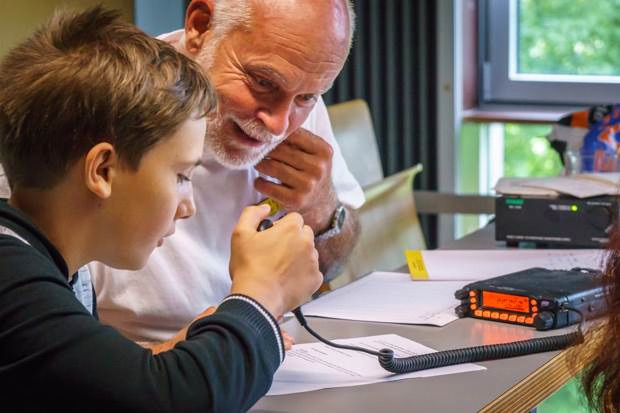
\includegraphics[width=0.85\textwidth]{foto/57}
    \caption{\scriptsize Ausbildungsfunkbetrieb verbindet oft die Generationen}
    \label{n_ausbildungsrufzeichen_ausbildungsfunkbetrieb}
\end{figure}

    \end{column}
   \begin{column}{0.48\textwidth}
       \begin{itemize}
  \item Funkamateure der Klasse~E und A sind automatisch Ausbilder
  \item Unter Aufsicht
  \item Im Berechtigungsumfang des Ausbilders
  \item Personengebundenes Rufzeichen + \enquote{/T} bzw. \enquote{/Trainee}
  \item Klubstation + \enquote{/T} bzw. \enquote{/Trainee}
  \end{itemize}

   \end{column}
\end{columns}

\end{frame}

\begin{frame}
\only<1>{
\begin{QQuestion}{VD302}{Unter welcher Voraussetzung nach der Amateurfunkverordnung (AFuV) darf ein Funkamateur Ausbildungsfunkbetrieb durchführen?}{Nur wenn er Inhaber einer Zulassung zur Teilnahme am Amateurfunkdienst der Klasse A ist}
{Wenn er Inhaber einer Zulassung zur Teilnahme am Amateurfunkdienst der Klasse A oder E ist}
{Nur wenn er mindestens 1 Jahr lang Inhaber einer Zulassung zur Teilnahme am Amateurfunkdienst ist}
{Wenn er eine gültige Rufzeichenzuteilung für ein Ausbildungsrufzeichen besitzt}
\end{QQuestion}

}
\only<2>{
\begin{QQuestion}{VD302}{Unter welcher Voraussetzung nach der Amateurfunkverordnung (AFuV) darf ein Funkamateur Ausbildungsfunkbetrieb durchführen?}{Nur wenn er Inhaber einer Zulassung zur Teilnahme am Amateurfunkdienst der Klasse A ist}
{\textbf{\textcolor{DARCgreen}{Wenn er Inhaber einer Zulassung zur Teilnahme am Amateurfunkdienst der Klasse A oder E ist}}}
{Nur wenn er mindestens 1 Jahr lang Inhaber einer Zulassung zur Teilnahme am Amateurfunkdienst ist}
{Wenn er eine gültige Rufzeichenzuteilung für ein Ausbildungsrufzeichen besitzt}
\end{QQuestion}

}
\end{frame}

\begin{frame}
\only<1>{
\begin{QQuestion}{BD211}{DG2RON führt Ausbildungsfunkbetrieb in Morsetelegrafie oder mit digitalen Übertragungsverfahren durch. Welches Rufzeichen hat der Auzubildende zu verwenden?}{DG2RON/A}
{T/DG2RON}
{DG2RON/T}
{A/DG2RON}
\end{QQuestion}

}
\only<2>{
\begin{QQuestion}{BD211}{DG2RON führt Ausbildungsfunkbetrieb in Morsetelegrafie oder mit digitalen Übertragungsverfahren durch. Welches Rufzeichen hat der Auzubildende zu verwenden?}{DG2RON/A}
{T/DG2RON}
{\textbf{\textcolor{DARCgreen}{DG2RON/T}}}
{A/DG2RON}
\end{QQuestion}

}
\end{frame}

\begin{frame}
\only<1>{
\begin{QQuestion}{VD304}{Was ist unter anderem im Zusammenhang mit der Durchführung von Ausbildungsfunkverkehr zu beachten? Der Ausbildungsfunkbetrieb darf~...}{nur mit einer maximalen Strahlungsleistung von \qty{10}{\W} EIRP durchgeführt werden.}
{nicht in Morsetelegrafie durchgeführt werden.}
{nur im Berechtigungsumfang der Rufzeichenzuteilung des Ausbilders durchgeführt werden.}
{nur an einer Klubstation durchgeführt werden.}
\end{QQuestion}

}
\only<2>{
\begin{QQuestion}{VD304}{Was ist unter anderem im Zusammenhang mit der Durchführung von Ausbildungsfunkverkehr zu beachten? Der Ausbildungsfunkbetrieb darf~...}{nur mit einer maximalen Strahlungsleistung von \qty{10}{\W} EIRP durchgeführt werden.}
{nicht in Morsetelegrafie durchgeführt werden.}
{\textbf{\textcolor{DARCgreen}{nur im Berechtigungsumfang der Rufzeichenzuteilung des Ausbilders durchgeführt werden.}}}
{nur an einer Klubstation durchgeführt werden.}
\end{QQuestion}

}
\end{frame}

\begin{frame}
\only<1>{
\begin{QQuestion}{BD210}{An der Klubstation DL0MOL soll Ausbildungsfunkbetrieb stattfinden. Darf der Auszubildende das Rufzeichen der Klubstation verwenden?}{Nein, es ist das persönliche Rufzeichen des Ausbilders zu verwenden.}
{Ja, wenn T/DL0MOL bzw. Trainee/DL0MOL verwendet wird.}
{Ja, wenn DL0MOL/T bzw. DL0MOL/Trainee verwendet wird.}
{Nein, an Klubstationen darf nicht ausgebildet werden.}
\end{QQuestion}

}
\only<2>{
\begin{QQuestion}{BD210}{An der Klubstation DL0MOL soll Ausbildungsfunkbetrieb stattfinden. Darf der Auszubildende das Rufzeichen der Klubstation verwenden?}{Nein, es ist das persönliche Rufzeichen des Ausbilders zu verwenden.}
{Ja, wenn T/DL0MOL bzw. Trainee/DL0MOL verwendet wird.}
{\textbf{\textcolor{DARCgreen}{Ja, wenn DL0MOL/T bzw. DL0MOL/Trainee verwendet wird.}}}
{Nein, an Klubstationen darf nicht ausgebildet werden.}
\end{QQuestion}

}
 \end{frame}

\begin{frame}
\frametitle{Ausbildungsfunkbetrieb ist …}
\begin{itemize}
  \item für Personen ohne Besitz eines entsprechenden Amateurfunkzeugnisses
  \item nicht für Aussendungen des Ausbilders selbst
  \item die praktische Vorbereitung auf das Ablegen der fachlichen Prüfung
  \end{itemize}
\end{frame}

\begin{frame}
\only<1>{
\begin{QQuestion}{VD301}{Wozu dient der Ausbildungsfunkbetrieb gemäß Amateurfunkverordnung (AFuV)? Er dient~...}{der alleinigen Vorführung des Amateurfunkbetriebes.}
{der praktischen Vorbereitung auf das Ablegen der fachlichen Prüfung zum Erwerb eines Amateurfunkzeugnisses.}
{der Teilnahme des Auszubildenden am Amateurfunkdienst ohne Aufsicht.}
{der Vervollständigung der Fertigkeiten des Funkamateurs in der Morsetelegrafie.}
\end{QQuestion}

}
\only<2>{
\begin{QQuestion}{VD301}{Wozu dient der Ausbildungsfunkbetrieb gemäß Amateurfunkverordnung (AFuV)? Er dient~...}{der alleinigen Vorführung des Amateurfunkbetriebes.}
{\textbf{\textcolor{DARCgreen}{der praktischen Vorbereitung auf das Ablegen der fachlichen Prüfung zum Erwerb eines Amateurfunkzeugnisses.}}}
{der Teilnahme des Auszubildenden am Amateurfunkdienst ohne Aufsicht.}
{der Vervollständigung der Fertigkeiten des Funkamateurs in der Morsetelegrafie.}
\end{QQuestion}

}
\end{frame}

\begin{frame}
\frametitle{Ausbilder …}
\begin{itemize}
  \item muss in unmittelbarer Nähe des Auszubildenden sein
  \item bei Bedienung und Betriebsabwicklung anleiten
  \item schaltet den Sender im Extremfall ab
  \item muss auf Verlangen der BNetzA Auskunft über \enquote{Art und Umfang} des Ausbildungsbetriebs geben
  \end{itemize}

\end{frame}

\begin{frame}
\only<1>{
\begin{QQuestion}{VD305}{Was ist bei der Durchführung von Ausbildungsfunkverkehr zu beachten?}{Der Ausbildungsfunkverkehr darf ausschließlich in Telefonie (SSB oder FM) durchgeführt werden.}
{Beim Ausbildungsfunkverkehr darf nicht an Amateurfunkwettbewerben teilgenommen werden.}
{Der Ausbildungsfunkverkehr darf ausschließlich in Gegenwart des Ausbilders an einer Klub- oder Schulstation durchgeführt werden.}
{Der  Ausbilder  hat  auf  Verlangen  der  Bundesnetzagentur  Auskunft  über  Art  und  Umfang  des 
Ausbildungsfunkbetriebs zu geben.}
\end{QQuestion}

}
\only<2>{
\begin{QQuestion}{VD305}{Was ist bei der Durchführung von Ausbildungsfunkverkehr zu beachten?}{Der Ausbildungsfunkverkehr darf ausschließlich in Telefonie (SSB oder FM) durchgeführt werden.}
{Beim Ausbildungsfunkverkehr darf nicht an Amateurfunkwettbewerben teilgenommen werden.}
{Der Ausbildungsfunkverkehr darf ausschließlich in Gegenwart des Ausbilders an einer Klub- oder Schulstation durchgeführt werden.}
{\textbf{\textcolor{DARCgreen}{Der  Ausbilder  hat  auf  Verlangen  der  Bundesnetzagentur  Auskunft  über  Art  und  Umfang  des 
Ausbildungsfunkbetriebs zu geben.}}}
\end{QQuestion}

}
 \end{frame}%ENDCONTENT


\section{Remote-Stationen}
\label{section:remote_stationen}
\begin{frame}%STARTCONTENT
\begin{itemize}
  \item Remotestationen ermöglichen einen Betrieb an einem anderen Standort
  \item z.B. wenn am Wohnort keine eigene Station realisiert werden kann
  \item Die gesamte Bedienung erfolgt ferngesteuert
  \end{itemize}
\begin{itemize}
  \item Betrieb durch Funkamateure der Klasse~A
  \item Mitbenutzung möglich
  \end{itemize}

\end{frame}

\begin{frame}
\only<1>{
\begin{QQuestion}{VD601}{Was versteht der Funkamateur unter \glqq Remote-Betrieb\grqq{}?}{Funkbetrieb bei Wettbewerben mit mehreren Funkamateuren mit verteilten Aufgaben}
{Funkbetrieb über sehr weite Entfernungen (größer \qty{500}{\km} UKW, größer \qty{2000}{\km} KW)}
{Die lokale Steuerung einer Funkstation über einen daneben stehenden Computer}
{Funkbetrieb, bei dem eine räumlich entfernte Amateurfunkstation z.~B. über das Internet betrieben wird}
\end{QQuestion}

}
\only<2>{
\begin{QQuestion}{VD601}{Was versteht der Funkamateur unter \glqq Remote-Betrieb\grqq{}?}{Funkbetrieb bei Wettbewerben mit mehreren Funkamateuren mit verteilten Aufgaben}
{Funkbetrieb über sehr weite Entfernungen (größer \qty{500}{\km} UKW, größer \qty{2000}{\km} KW)}
{Die lokale Steuerung einer Funkstation über einen daneben stehenden Computer}
{\textbf{\textcolor{DARCgreen}{Funkbetrieb, bei dem eine räumlich entfernte Amateurfunkstation z.~B. über das Internet betrieben wird}}}
\end{QQuestion}

}
\end{frame}

\begin{frame}
\only<1>{
\begin{QQuestion}{VD603}{Wer darf eine \glqq Remote-Station\grqq{} betreiben?}{Funkamateure der Klassen A und E}
{Funkamateure der Klasse A}
{Funkamateure der Klassen A, E und N}
{Funkamateure, die seit mindestens einem Jahr eine Zulassung besitzen}
\end{QQuestion}

}
\only<2>{
\begin{QQuestion}{VD603}{Wer darf eine \glqq Remote-Station\grqq{} betreiben?}{Funkamateure der Klassen A und E}
{\textbf{\textcolor{DARCgreen}{Funkamateure der Klasse A}}}
{Funkamateure der Klassen A, E und N}
{Funkamateure, die seit mindestens einem Jahr eine Zulassung besitzen}
\end{QQuestion}

}
\end{frame}

\begin{frame}
\only<1>{
\begin{QQuestion}{VD607}{Wer darf mit einer Amateurfunkstelle im \glqq Remote-Betrieb\grqq{} senden? Vom Betreiber der Amateurfunkstelle berechtigte Funkamateure, die ...}{über eine Zulassung für die Klasse~A, E oder N verfügen.}
{über eine Zulassung für die Klasse~A oder E verfügen.}
{über eine Zulassung für die Klasse~A verfügen.}
{seit mindestens einem Jahr über eine Zulassung verfügen.}
\end{QQuestion}

}
\only<2>{
\begin{QQuestion}{VD607}{Wer darf mit einer Amateurfunkstelle im \glqq Remote-Betrieb\grqq{} senden? Vom Betreiber der Amateurfunkstelle berechtigte Funkamateure, die ...}{über eine Zulassung für die Klasse~A, E oder N verfügen.}
{über eine Zulassung für die Klasse~A oder E verfügen.}
{\textbf{\textcolor{DARCgreen}{über eine Zulassung für die Klasse~A verfügen.}}}
{seit mindestens einem Jahr über eine Zulassung verfügen.}
\end{QQuestion}

}
\end{frame}

\begin{frame}
\frametitle{Betriebsmeldung}
\begin{itemize}
  \item Remotebetrieb muss durch den Betreiber angezeigt werden
  \item Mit Betriebsmeldung und Kontaktdaten an die BNetzA
  \item Erreichbarkeit während des Betriebs unter den angegebenen Kontaktdaten
  \end{itemize}

\end{frame}

\begin{frame}
\only<1>{
\begin{QQuestion}{VD602}{Ist für \glqq Remote-Betrieb\grqq{} bei der BNetzA eine Betriebsmeldung erforderlich?}{Ja, für Betreiber und Nutzer der Remote-Station}
{Ja, für den Nutzer der Remote-Station}
{Ja, für den Betreiber der Remote-Station}
{Nein, es besteht keine Anzeigepflicht.}
\end{QQuestion}

}
\only<2>{
\begin{QQuestion}{VD602}{Ist für \glqq Remote-Betrieb\grqq{} bei der BNetzA eine Betriebsmeldung erforderlich?}{Ja, für Betreiber und Nutzer der Remote-Station}
{Ja, für den Nutzer der Remote-Station}
{\textbf{\textcolor{DARCgreen}{Ja, für den Betreiber der Remote-Station}}}
{Nein, es besteht keine Anzeigepflicht.}
\end{QQuestion}

}
\end{frame}

\begin{frame}
\only<1>{
\begin{QQuestion}{VD608}{Warum muss der Betreiber der \glqq Remote-Station\grqq{} seine Kontaktdaten bei der BNetzA angeben?}{Die Bandwacht der Amateurfunkverbände nutzt die Kontaktdaten zum Datenabgleich, um im Störungsfall den Betreiber der \glqq Remote-Station\grqq{} zu ermitteln.}
{Die Kontaktdaten dienen der monatlichen Rechnungsstellung für die \glqq Remote-Station\grqq{}.}
{Der Betreiber muss für die BNetzA als Ansprechpartner erreichbar sein.}
{Die Kontaktdaten zum Remote-Betrieb werden in der Rufzeichenliste der BNetzA aufgeführt.}
\end{QQuestion}

}
\only<2>{
\begin{QQuestion}{VD608}{Warum muss der Betreiber der \glqq Remote-Station\grqq{} seine Kontaktdaten bei der BNetzA angeben?}{Die Bandwacht der Amateurfunkverbände nutzt die Kontaktdaten zum Datenabgleich, um im Störungsfall den Betreiber der \glqq Remote-Station\grqq{} zu ermitteln.}
{Die Kontaktdaten dienen der monatlichen Rechnungsstellung für die \glqq Remote-Station\grqq{}.}
{\textbf{\textcolor{DARCgreen}{Der Betreiber muss für die BNetzA als Ansprechpartner erreichbar sein.}}}
{Die Kontaktdaten zum Remote-Betrieb werden in der Rufzeichenliste der BNetzA aufgeführt.}
\end{QQuestion}

}
\end{frame}

\begin{frame}
\frametitle{Betriebssicherheit}
\begin{itemize}
  \item Ununterbrochene, mittelbare und vollständige Kontrolle der Station
  \item Kann über Hilfsmittel oder Helfer erfolgen
  \item Bei Störungen muss die Stationen in einen sicheren Zustand versetzt werden
  \end{itemize}

\end{frame}

\begin{frame}
\only<1>{
\begin{QQuestion}{VD605}{Wie muss der Betreiber die Betriebssicherheit seiner \glqq Remote-Station\grqq{} gewährleisten? Der Betreiber muss sicherstellen, dass~...}{die \glqq Remote-Station\grqq{} über eine unterbrechungsfreie Stromversorgung verfügt.}
{für die \glqq Remote-Station\grqq{} keine selbstgebauten Komponenten zum Einsatz kommen.}
{die \glqq Remote-Station\grqq{} unter seiner mittelbaren Kontrolle steht.}
{ein technisches Protokoll der Nutzung der \glqq Remote-Station\grqq{} erstellt wird.}
\end{QQuestion}

}
\only<2>{
\begin{QQuestion}{VD605}{Wie muss der Betreiber die Betriebssicherheit seiner \glqq Remote-Station\grqq{} gewährleisten? Der Betreiber muss sicherstellen, dass~...}{die \glqq Remote-Station\grqq{} über eine unterbrechungsfreie Stromversorgung verfügt.}
{für die \glqq Remote-Station\grqq{} keine selbstgebauten Komponenten zum Einsatz kommen.}
{\textbf{\textcolor{DARCgreen}{die \glqq Remote-Station\grqq{} unter seiner mittelbaren Kontrolle steht.}}}
{ein technisches Protokoll der Nutzung der \glqq Remote-Station\grqq{} erstellt wird.}
\end{QQuestion}

}
\end{frame}

\begin{frame}
\frametitle{Berechtigte Funkamateure}
\begin{itemize}
  \item Erlaubnis des Betreibers für Nutzung notwendig
  \item Betreiber darf nur berechtigte Funkamateure die Remotestation nutzen lassen
  \end{itemize}
\end{frame}

\begin{frame}
\only<1>{
\begin{QQuestion}{VD606}{Was ist bei der Übertragung des Nutzungsrechts an einer \glqq Remote-Station\grqq{} auf andere Funkamateure zu beachten?}{Der Betreiber muss sicherstellen, dass nur von ihm berechtigte Funkamateure die Station nutzen können.}
{Der Zugang für die Nutzung der \glqq Remote-Station\grqq{} muss für alle Funkamateure öffentlich sein.}
{Die Nutzer der \glqq Remote-Station\grqq{} dürfen keinen Ausbildungsfunkbetrieb durchführen.}
{Die Funkamateure müssen mindestens im Besitz einer Amateurfunkzulassung der Klasse~E sein.}
\end{QQuestion}

}
\only<2>{
\begin{QQuestion}{VD606}{Was ist bei der Übertragung des Nutzungsrechts an einer \glqq Remote-Station\grqq{} auf andere Funkamateure zu beachten?}{\textbf{\textcolor{DARCgreen}{Der Betreiber muss sicherstellen, dass nur von ihm berechtigte Funkamateure die Station nutzen können.}}}
{Der Zugang für die Nutzung der \glqq Remote-Station\grqq{} muss für alle Funkamateure öffentlich sein.}
{Die Nutzer der \glqq Remote-Station\grqq{} dürfen keinen Ausbildungsfunkbetrieb durchführen.}
{Die Funkamateure müssen mindestens im Besitz einer Amateurfunkzulassung der Klasse~E sein.}
\end{QQuestion}

}
\end{frame}

\begin{frame}
\frametitle{Klubstationen}
\begin{itemize}
  \item Klubstationen der Klasse~A dürfen als Remotestation betrieben werden
  \item Muss auf die Mitglieder der Gruppe von Funkamateuren begrenzt sein
  \end{itemize}
\end{frame}

\begin{frame}
\only<1>{
\begin{QQuestion}{VD604}{Welche der folgenden Amateurfunkstellen darf als \glqq Remote-Station\grqq{} verwendet werden?}{Amateurfunkstellen mit personengebundenem Rufzeichen der Klasse~N}
{Klubstationen der Klasse~E}
{Klubstationen der Klasse~A}
{Amateurfunkstellen mit personengebundenem Rufzeichen der Klasse~E}
\end{QQuestion}

}
\only<2>{
\begin{QQuestion}{VD604}{Welche der folgenden Amateurfunkstellen darf als \glqq Remote-Station\grqq{} verwendet werden?}{Amateurfunkstellen mit personengebundenem Rufzeichen der Klasse~N}
{Klubstationen der Klasse~E}
{\textbf{\textcolor{DARCgreen}{Klubstationen der Klasse~A}}}
{Amateurfunkstellen mit personengebundenem Rufzeichen der Klasse~E}
\end{QQuestion}

}
\end{frame}

\begin{frame}
\only<1>{
\begin{QQuestion}{VD609}{Wem darf Zugriff auf eine Klubstation im Remote-Betrieb eingeräumt werden?}{Nur Mitgliedern der Gruppe von Funkamateuren, die die Klubstation betreibt}
{Nur auf der Zuteilungsurkunde eingetragenen Mitgliedern der Gruppe von Funkamateuren}
{Nur bei der Bundesnetzagentur schriftlich oder elektronisch gemeldeten Funkamateuren}
{Nur Funkamateuren, die die Klubstation persönlich nicht aufsuchen können}
\end{QQuestion}

}
\only<2>{
\begin{QQuestion}{VD609}{Wem darf Zugriff auf eine Klubstation im Remote-Betrieb eingeräumt werden?}{\textbf{\textcolor{DARCgreen}{Nur Mitgliedern der Gruppe von Funkamateuren, die die Klubstation betreibt}}}
{Nur auf der Zuteilungsurkunde eingetragenen Mitgliedern der Gruppe von Funkamateuren}
{Nur bei der Bundesnetzagentur schriftlich oder elektronisch gemeldeten Funkamateuren}
{Nur Funkamateuren, die die Klubstation persönlich nicht aufsuchen können}
\end{QQuestion}

}
\end{frame}

\begin{frame}
\frametitle{Ausbildungsfunkbetrieb}
\begin{itemize}
  \item Ist an einer Remotestation möglich
  \item Es gelten die gleichen Regeln wie für den Ausbildungsbetrieb
  \item Auch an Remote-Klubstationen möglich
  \end{itemize}

\end{frame}%ENDCONTENT


\section{Rufzeichenzusätze}
\label{section:rufzeichenzusaetze}
\begin{frame}%STARTCONTENT
Beim Funken von einem Standort anders als dem in der Zulassungsurkunde angegebenen Heimatstandort, kann ein Rufzeichenzusatz verwendet werden.

\end{frame}

\begin{frame}\begin{table}
\begin{DARCtabular}{lll}
     Zusatz  & Gesprochen  & Bedeutung   \\
     am  & aeronautisch mobil  & An Bord eines Luftfahrzeugst, das sich im Flug befindet   \\
     mm  & maritim mobil  & An Bord eines Schiffs auf See   \\
     m  & mobil  & Von einem Landfahrzeug oder einem Schiff auf Binnengewässern aus   \\
     p  & portabel  & Zu Fuß unterwegs oder vorübergehend ortsfest   \\
     R  & Remote  & Remote-Betrieb   \\
     T  & Trainee  & Ausbildungsfunk   \\
\end{DARCtabular}
\caption{Mögliche Rufzeichenzusätze}
\label{n_rufzeichenzusaetze}
\end{table}

\end{frame}

\begin{frame}\begin{itemize}
  \item Geschrieben mit \enquote{/}
  \item Gesprochen direkt im Anschluss an das Rufzeichen oder mit \enquote{Stroke}
  \end{itemize}
    \pause
    \begin{table}
\begin{DARCtabular}{lX}
     Schreibweise  & Aussprache   \\
     DL1FLO/m  & Delta Lima Eins Foxtrott Lima Oskar (Stroke) Mobil   \\
     DM4EAX/p  & Delta Mike Vier Echo Alpha X-Ray (Stroke) Portabel   \\
     DL1ASN/mm  & Delta Lima Eins Alpha Sierra November (Stroke) Maritim Mobil   \\
     DG2RON/am  & Delta Golf Zwei Romeo Oscar November (Stroke) Aeronautisch Mobil   \\
\end{DARCtabular}
\caption{Sprechweise von Rufzeichenzusätzen, "Stroke" ist optional und kann weggelassen werden}
\label{n_rufzeichenzusaetze_sprechweise}
\end{table}


\end{frame}

\begin{frame}
\frametitle{Aeronautisch Mobil}
\begin{itemize}
  \item An Bord eines Luftfahrzeugs (Flugzeug, Heißluftballon, Zeppelin, o.ä.)
  \item Muss sich komplett in der Luft befinden
  \item Keine Verbindung zum Boden
  \item Betrieb muss vom Luftfahrzeugführer erlaubt sein, jedoch nicht von der BNetzA genehmigt werden
  \end{itemize}
\end{frame}

\begin{frame}
\only<1>{
\begin{QQuestion}{BD201}{Was bedeutet der Rufzeichenzusatz \glqq /am\grqq{}? Die Amateurfunkstelle~...}{verwendet Amplitudenmodulation.}
{wird an Bord eines Luftfahrzeugs betrieben.}
{wird an Bord eines Wasserfahrzeugs betrieben.}
{arbeitet mit geringer Leistung.}
\end{QQuestion}

}
\only<2>{
\begin{QQuestion}{BD201}{Was bedeutet der Rufzeichenzusatz \glqq /am\grqq{}? Die Amateurfunkstelle~...}{verwendet Amplitudenmodulation.}
{\textbf{\textcolor{DARCgreen}{wird an Bord eines Luftfahrzeugs betrieben.}}}
{wird an Bord eines Wasserfahrzeugs betrieben.}
{arbeitet mit geringer Leistung.}
\end{QQuestion}

}
\end{frame}

\begin{frame}
\only<1>{
\begin{QQuestion}{BD202}{Welche Bedeutung hat das Rufzeichen VE8ZZ/am?}{Es handelt sich um eine kanadische Amateurfunkstelle, die vorübergehend in den Vereinigten Staaten von Amerika betrieben wird.}
{Es handelt sich um eine Amateurfunkstelle mit einem kanadischen Rufzeichen, die in einem Luftfahrzeug betrieben wird.}
{Es handelt sich um eine kanadische Amateurfunkstelle, die in der Modulationsart AM betrieben wird.}
{Es handelt sich um eine automatisch arbeitende Pactor-Amateurfunkstelle mit angeschlossener Mailbox in Kanada.}
\end{QQuestion}

}
\only<2>{
\begin{QQuestion}{BD202}{Welche Bedeutung hat das Rufzeichen VE8ZZ/am?}{Es handelt sich um eine kanadische Amateurfunkstelle, die vorübergehend in den Vereinigten Staaten von Amerika betrieben wird.}
{\textbf{\textcolor{DARCgreen}{Es handelt sich um eine Amateurfunkstelle mit einem kanadischen Rufzeichen, die in einem Luftfahrzeug betrieben wird.}}}
{Es handelt sich um eine kanadische Amateurfunkstelle, die in der Modulationsart AM betrieben wird.}
{Es handelt sich um eine automatisch arbeitende Pactor-Amateurfunkstelle mit angeschlossener Mailbox in Kanada.}
\end{QQuestion}

}
\end{frame}

\begin{frame}
\only<1>{
\begin{QQuestion}{VE705}{Welche Voraussetzung muss erfüllt sein, damit Sie Amateurfunk an Bord eines Luftfahrzeugs betreiben dürfen?}{Genehmigung der Bundesnetzagentur für aeronautischen Funkbetrieb}
{Zustimmung des verantwortlichen Luftfahrzeugführers}
{Verwendung einer fest installierten Funkstelle des mobilen Flugfunkdienstes}
{Nutzung von Frequenzen, die dem mobilen Flugfunkdienst zugewiesen sind}
\end{QQuestion}

}
\only<2>{
\begin{QQuestion}{VE705}{Welche Voraussetzung muss erfüllt sein, damit Sie Amateurfunk an Bord eines Luftfahrzeugs betreiben dürfen?}{Genehmigung der Bundesnetzagentur für aeronautischen Funkbetrieb}
{\textbf{\textcolor{DARCgreen}{Zustimmung des verantwortlichen Luftfahrzeugführers}}}
{Verwendung einer fest installierten Funkstelle des mobilen Flugfunkdienstes}
{Nutzung von Frequenzen, die dem mobilen Flugfunkdienst zugewiesen sind}
\end{QQuestion}

}
\end{frame}

\begin{frame}
\frametitle{Maritim Mobil}
\begin{itemize}
  \item An Bord eines Wasserfahrzeugs (Motorboot, Segelyacht, o.ä.)
  \item Außerhalb der 12-Meilen-Zone
  \item Auf Flüssen, Seen oder ähnlichen Binnengewässern darf \enquote{/m} (mobil) verwendet werden
  \item Betrieb muss vom Schiffsführer erlaubt sein, jedoch nicht von der BNetzA genehmigt werden
  \end{itemize}
\end{frame}

\begin{frame}
\only<1>{
\begin{QQuestion}{BD205}{Was ist aus dem Rufzeichen DC4LW/mm hinsichtlich des Betriebsortes zu erkennen? Die deutsche Amateurfunkstelle DC4LW~...}{wird von einem Schiff aus betrieben, das sich auf einem Binnengewässer befindet.}
{wird an Bord eines Wasserfahrzeugs betrieben, das sich auf See befindet.}
{möchte mit anderen Funkamateuren in Kontakt treten, die ihre Funkstelle zur Zeit auch \glqq maritim mobil\grqq{} betreiben.}
{wird an Bord eines Schiffes als eine mobile Station des See- und Binnenschifffahrtsfunks betrieben.}
\end{QQuestion}

}
\only<2>{
\begin{QQuestion}{BD205}{Was ist aus dem Rufzeichen DC4LW/mm hinsichtlich des Betriebsortes zu erkennen? Die deutsche Amateurfunkstelle DC4LW~...}{wird von einem Schiff aus betrieben, das sich auf einem Binnengewässer befindet.}
{\textbf{\textcolor{DARCgreen}{wird an Bord eines Wasserfahrzeugs betrieben, das sich auf See befindet.}}}
{möchte mit anderen Funkamateuren in Kontakt treten, die ihre Funkstelle zur Zeit auch \glqq maritim mobil\grqq{} betreiben.}
{wird an Bord eines Schiffes als eine mobile Station des See- und Binnenschifffahrtsfunks betrieben.}
\end{QQuestion}

}
\end{frame}

\begin{frame}
\only<1>{
\begin{QQuestion}{VE706}{Darf eine Amateurfunkstelle auch an Bord eines Schiffes, welches sich in internationalen Gewässern befindet, betrieben werden?}{Ja, mit der Zustimmung des Schiffsführers}
{Ja, mit der Zustimmung eines beliebigen Crewmitglieds}
{Ja, mit einer Genehmigung der BNetzA}
{Ja, mit einer Genehmigung des Bundesamtes für Seeschifffahrt und Hydrographie}
\end{QQuestion}

}
\only<2>{
\begin{QQuestion}{VE706}{Darf eine Amateurfunkstelle auch an Bord eines Schiffes, welches sich in internationalen Gewässern befindet, betrieben werden?}{\textbf{\textcolor{DARCgreen}{Ja, mit der Zustimmung des Schiffsführers}}}
{Ja, mit der Zustimmung eines beliebigen Crewmitglieds}
{Ja, mit einer Genehmigung der BNetzA}
{Ja, mit einer Genehmigung des Bundesamtes für Seeschifffahrt und Hydrographie}
\end{QQuestion}

}
\end{frame}

\begin{frame}
\only<1>{
\begin{QQuestion}{VD115}{Ist für den Betrieb einer Amateurfunkstelle in einem Wasser- oder Luftfahrzeug eine Sondergenehmigung der Bundesnetzagentur erforderlich?}{Es ist keine Sondergenehmigung  erforderlich.}
{Wenn der Funkamateur auch Inhaber eines Flugfunk- oder Seefunkzeugnisses ist, benötigt er keine Sondergenehmigung.}
{Es ist in jedem Fall eine Sondergenehmigung erforderlich.}
{Bei Strahlungsleistungen von über \qty{10}{\W} EIRP ist eine Sondergenehmigung erforderlich.}
\end{QQuestion}

}
\only<2>{
\begin{QQuestion}{VD115}{Ist für den Betrieb einer Amateurfunkstelle in einem Wasser- oder Luftfahrzeug eine Sondergenehmigung der Bundesnetzagentur erforderlich?}{\textbf{\textcolor{DARCgreen}{Es ist keine Sondergenehmigung  erforderlich.}}}
{Wenn der Funkamateur auch Inhaber eines Flugfunk- oder Seefunkzeugnisses ist, benötigt er keine Sondergenehmigung.}
{Es ist in jedem Fall eine Sondergenehmigung erforderlich.}
{Bei Strahlungsleistungen von über \qty{10}{\W} EIRP ist eine Sondergenehmigung erforderlich.}
\end{QQuestion}

}
\end{frame}

\begin{frame}
\frametitle{Mobil}
\begin{itemize}
  \item In einem Landfahrzeug wie Auto oder Zug
  \item Oder an Bord eines Schiffs auf Binnengewässern
  \end{itemize}
\end{frame}

\begin{frame}
\only<1>{
\begin{QQuestion}{BD203}{Ein Rufzeichen mit dem Zusatz \glqq /m\grqq{} kann bei einer Amateurfunkstelle bedeuten, dass sie~...}{vorübergehend ortsfest betrieben wird oder tragbar ist.}
{mit minimaler Leistung sendet.}
{beweglich ist und sich in einem Landfahrzeug befindet.}
{an Bord eines Wasserfahrzeugs betrieben wird, das sich auf See befindet.}
\end{QQuestion}

}
\only<2>{
\begin{QQuestion}{BD203}{Ein Rufzeichen mit dem Zusatz \glqq /m\grqq{} kann bei einer Amateurfunkstelle bedeuten, dass sie~...}{vorübergehend ortsfest betrieben wird oder tragbar ist.}
{mit minimaler Leistung sendet.}
{\textbf{\textcolor{DARCgreen}{beweglich ist und sich in einem Landfahrzeug befindet.}}}
{an Bord eines Wasserfahrzeugs betrieben wird, das sich auf See befindet.}
\end{QQuestion}

}
\end{frame}

\begin{frame}
\only<1>{
\begin{QQuestion}{BD204}{Ein Rufzeichen mit dem Zusatz \glqq /m\grqq{} kann bei einer Amateurfunkstelle bedeuten, dass sie~...}{an Bord eines Wasserfahrzeugs betrieben wird, das sich auf See befindet.}
{mit minimaler Leistung sendet.}
{vorübergehend ortsfest betrieben wird oder tragbar ist.}
{sich an Bord eines Wasserfahrzeugs auf Binnengewässern befindet.}
\end{QQuestion}

}
\only<2>{
\begin{QQuestion}{BD204}{Ein Rufzeichen mit dem Zusatz \glqq /m\grqq{} kann bei einer Amateurfunkstelle bedeuten, dass sie~...}{an Bord eines Wasserfahrzeugs betrieben wird, das sich auf See befindet.}
{mit minimaler Leistung sendet.}
{vorübergehend ortsfest betrieben wird oder tragbar ist.}
{\textbf{\textcolor{DARCgreen}{sich an Bord eines Wasserfahrzeugs auf Binnengewässern befindet.}}}
\end{QQuestion}

}
\end{frame}

\begin{frame}
\frametitle{Portabel}
\begin{itemize}
  \item Station vorübergehend an einem Standort, der nicht auf der Zuteilungsurkunde eingetragen ist
  \item z.B. in der Natur
  \item Auch bei Bewegung (zu Fuß) mit tragbarem Funkgerät
  \end{itemize}
\end{frame}

\begin{frame}
\only<1>{
\begin{QQuestion}{BD206}{Was bedeutet der Rufzeichenzusatz \glqq /p\grqq{}? Es bedeutet, dass die Amateurfunkstelle~...}{sich an Bord eines Wasserfahrzeugs auf See befindet.}
{sich in einem Landfahrzeug in Bewegung befindet.}
{vorübergehend exterritorial betrieben wird.}
{vorübergehend ortsfest betrieben wird oder tragbar ist.}
\end{QQuestion}

}
\only<2>{
\begin{QQuestion}{BD206}{Was bedeutet der Rufzeichenzusatz \glqq /p\grqq{}? Es bedeutet, dass die Amateurfunkstelle~...}{sich an Bord eines Wasserfahrzeugs auf See befindet.}
{sich in einem Landfahrzeug in Bewegung befindet.}
{vorübergehend exterritorial betrieben wird.}
{\textbf{\textcolor{DARCgreen}{vorübergehend ortsfest betrieben wird oder tragbar ist.}}}
\end{QQuestion}

}
\end{frame}

\begin{frame}
\only<1>{
\begin{QQuestion}{BD207}{Muss beim Betrieb einer tragbaren oder vorübergehend ortsfest betriebenen Amateurfunkstelle in Deutschland dem Rufzeichen der Zusatz \glqq /p\grqq{} hinzugefügt werden?}{Nein, es sei denn, es handelt sich um eine ausländische Station.}
{Ja, damit die BNetzA erkennen kann, dass die Amateurfunkstelle nicht am gemeldeten Standort betrieben wird.}
{Ja, weil dies durch die internationalen Regelungen in den Radio Regulations (RR) so vorgegeben ist.}
{Nein, er kann zur weiteren Information verwendet werden.}
\end{QQuestion}

}
\only<2>{
\begin{QQuestion}{BD207}{Muss beim Betrieb einer tragbaren oder vorübergehend ortsfest betriebenen Amateurfunkstelle in Deutschland dem Rufzeichen der Zusatz \glqq /p\grqq{} hinzugefügt werden?}{Nein, es sei denn, es handelt sich um eine ausländische Station.}
{Ja, damit die BNetzA erkennen kann, dass die Amateurfunkstelle nicht am gemeldeten Standort betrieben wird.}
{Ja, weil dies durch die internationalen Regelungen in den Radio Regulations (RR) so vorgegeben ist.}
{\textbf{\textcolor{DARCgreen}{Nein, er kann zur weiteren Information verwendet werden.}}}
\end{QQuestion}

}
\end{frame}

\begin{frame}
\frametitle{Remote}
\begin{itemize}
  \item Betrieb an einer Remote-Station
  \item Optional \enquote{/R} bzw. \enquote{/Remote}
  \end{itemize}
\end{frame}

\begin{frame}
\only<1>{
\begin{QQuestion}{BD208}{Welcher Rufzeichenzusatz kann verwendet werden, um \glqq Remote-Betrieb\grqq{} zu kennzeichnen?}{/RB bzw. /Remotebetrieb}
{/R bzw. /Remote}
{/FB bzw. /Fernbedient}
{/F bzw. /Fern}
\end{QQuestion}

}
\only<2>{
\begin{QQuestion}{BD208}{Welcher Rufzeichenzusatz kann verwendet werden, um \glqq Remote-Betrieb\grqq{} zu kennzeichnen?}{/RB bzw. /Remotebetrieb}
{\textbf{\textcolor{DARCgreen}{/R bzw. /Remote}}}
{/FB bzw. /Fernbedient}
{/F bzw. /Fern}
\end{QQuestion}

}
\end{frame}

\begin{frame}
\frametitle{Trainee}
\begin{itemize}
  \item Bei Ausbildungsfunkbetrieb ist \enquote{/T} bzw. \enquote{/Trainee} verpflichtend
  \item Alle anderen Zusätze sind freiwillig und können weggelassen werden
  \end{itemize}
\end{frame}

\begin{frame}
\only<1>{
\begin{QQuestion}{BD209}{Der Funkamateur mit dem Rufzeichen DL1PZ möchte Ausbildungsfunkbetrieb im Sprechfunk durchführen. Welches Rufzeichen darf der Auszubildende verwenden?}{DL1PZ/Trainee}
{DL1PZ/Ausbildung}
{Ausbildung/DL1PZ}
{Trainee/DL1PZ}
\end{QQuestion}

}
\only<2>{
\begin{QQuestion}{BD209}{Der Funkamateur mit dem Rufzeichen DL1PZ möchte Ausbildungsfunkbetrieb im Sprechfunk durchführen. Welches Rufzeichen darf der Auszubildende verwenden?}{\textbf{\textcolor{DARCgreen}{DL1PZ/Trainee}}}
{DL1PZ/Ausbildung}
{Ausbildung/DL1PZ}
{Trainee/DL1PZ}
\end{QQuestion}

}
\end{frame}

\begin{frame}
\only<1>{
\begin{QQuestion}{VD306}{Von wem ist während des Ausbildungsfunkbetriebs der Rufzeichenzusatz \glqq /T\grqq{} bzw. \glqq /Trainee\grqq{} zu benutzen?}{Vom Verantwortlichen der Schulstation}
{Vom Ausbilder}
{Vom Auszubildenden und vom Ausbilder}
{Vom Auszubildenden}
\end{QQuestion}

}
\only<2>{
\begin{QQuestion}{VD306}{Von wem ist während des Ausbildungsfunkbetriebs der Rufzeichenzusatz \glqq /T\grqq{} bzw. \glqq /Trainee\grqq{} zu benutzen?}{Vom Verantwortlichen der Schulstation}
{Vom Ausbilder}
{Vom Auszubildenden und vom Ausbilder}
{\textbf{\textcolor{DARCgreen}{Vom Auszubildenden}}}
\end{QQuestion}

}
\end{frame}

\begin{frame}
\only<1>{
\begin{QQuestion}{BD210}{An der Klubstation DL0MOL soll Ausbildungsfunkbetrieb stattfinden. Darf der Auszubildende das Rufzeichen der Klubstation verwenden?}{Nein, es ist das persönliche Rufzeichen des Ausbilders zu verwenden.}
{Ja, wenn T/DL0MOL bzw. Trainee/DL0MOL verwendet wird.}
{Ja, wenn DL0MOL/T bzw. DL0MOL/Trainee verwendet wird.}
{Nein, an Klubstationen darf nicht ausgebildet werden.}
\end{QQuestion}

}
\only<2>{
\begin{QQuestion}{BD210}{An der Klubstation DL0MOL soll Ausbildungsfunkbetrieb stattfinden. Darf der Auszubildende das Rufzeichen der Klubstation verwenden?}{Nein, es ist das persönliche Rufzeichen des Ausbilders zu verwenden.}
{Ja, wenn T/DL0MOL bzw. Trainee/DL0MOL verwendet wird.}
{\textbf{\textcolor{DARCgreen}{Ja, wenn DL0MOL/T bzw. DL0MOL/Trainee verwendet wird.}}}
{Nein, an Klubstationen darf nicht ausgebildet werden.}
\end{QQuestion}

}
\end{frame}%ENDCONTENT


\section{Besondere Anlässe}
\label{section:besondere_anlaesse}
\begin{frame}%STARTCONTENT

\begin{columns}
    \begin{column}{0.48\textwidth}
    
\begin{figure}
    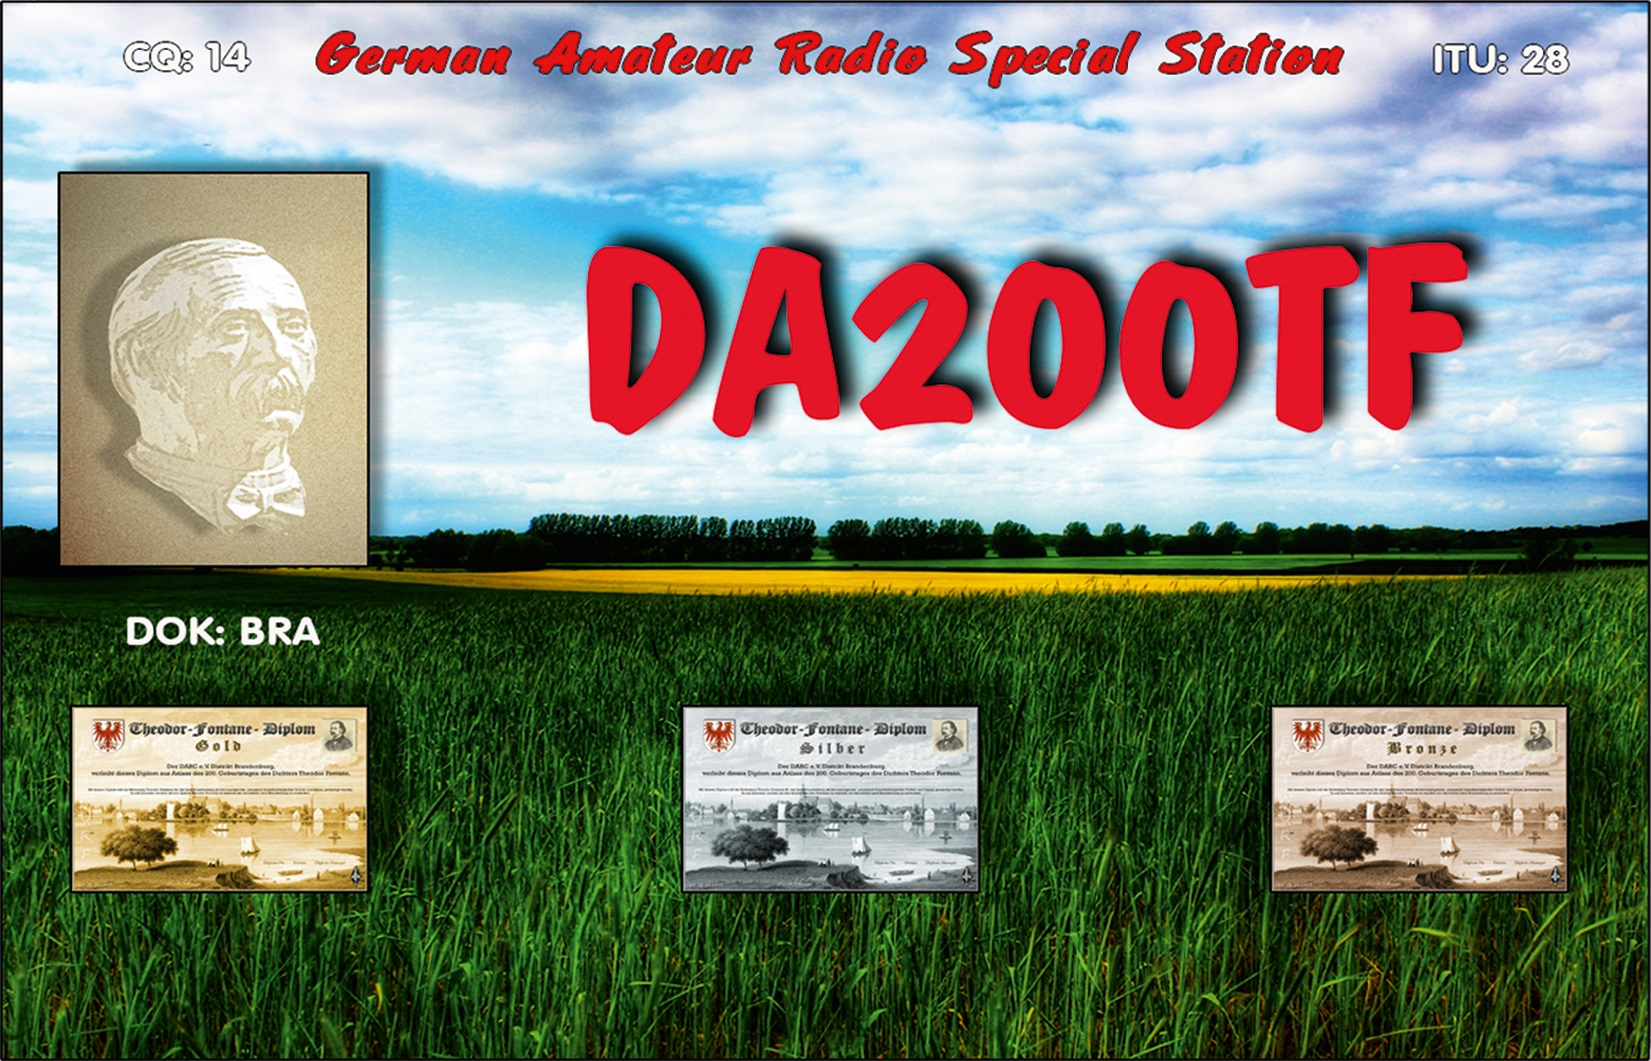
\includegraphics[width=0.85\textwidth]{foto/59}
    \caption{\scriptsize QSL-Karte der Klubstation mit dem Sonderrufzeichen DA200TF anlässlich des 200. Geburtstag von Theodor Fontane}
    \label{n_besondere_anlaesse_qsl_karte_DA200TF}
\end{figure}

    \end{column}
   \begin{column}{0.48\textwidth}
       \begin{itemize}
  \item Klubstationsrufzeichen mit 4-7stelligem Suffix
  \item z.B. für historische Ereignisse, Stadtfeste oder Sportereignisse
  \item Die ganze Amateurfunkwelt kann an dem Ereignis teilhaben
  \end{itemize}

   \end{column}
\end{columns}

\end{frame}

\begin{frame}
\frametitle{Vorgaben}
\begin{itemize}
  \item Maximale Zuweisung für 1 Jahr durch die BNetzA
  \item Keine Verlängerung möglich
  \item Suffix kann aus Ziffern und Buchstaben bestehen
  \item Das letzte Zeichen muss immer ein Buchstabe sein
  \end{itemize}
\end{frame}

\begin{frame}
\frametitle{International}
\begin{itemize}
  \item Auch im Ausland kann es Sonderstationen geben
  \item Die Rufzeichen können andere Vorgaben haben
  \end{itemize}
\end{frame}

\begin{frame}\begin{table}
\begin{DARCtabular}{llX}
     Rufzeichen  & Zuteilung  & Ereignis   \\
     DL1250BRET  & 2017  & 1250 Jahre Stadt Bretten   \\
     DL500BIER  & 2016  & 500 Jahre Deutsches Reinheitsgebot   \\
     DF13DEJU  & 2019  & Erstflug der Junkers F 13   \\
     DL73AFUG  & 2022  & 73. Geburtstags des Amateurfunkgesetzes   \\
     DB50AFZ  & 2022  & 50 Jahre Amateurfunkzentrum   \\
     DP44N44T  & 2022  & 44 Jahre Ortsverband N44   \\
     DC0YOTA  & 2021  & Youngsters On The Air   \\
     DL22MAUS  & 2022  & Türen auf mit der Maus!   \\
     DL0ELEFANT  & 2022  & Türen auf mit der Maus!   \\
\end{DARCtabular}
\caption{Beispiele für Sonderstationen}
\label{n_besondere_anlaesse}
\end{table}

\end{frame}

\begin{frame}
\only<1>{
\begin{QQuestion}{VD204}{Warum ist \glqq DL250BTHVN\grqq{} ein zulässiges deutsches Amateurfunkrufzeichen?}{Weil für besonders verdiente Funkamateure auch personengebundene Rufzeichen ausgegeben werden, für die der Rufzeichenplan keine Anwendung findet.}
{Weil der Rufzeichenplan zu besonderen allgemeinen Anlässen auch Rufzeichen mit bis zu 7 Zeichen langem Suffix vorsieht, der Ziffern enthalten kann und mit einem Buchstaben endet.}
{Weil an bestimmte öffentliche Stellen, wie z.~B. Kunst- und Kultureinrichtungen, besondere Rufzeichen mit mindestens 3 Ziffern ausgegeben werden.}
{Weil dies in einer Sonderverfügung der Bundesnetzagentur aufgrund besonderen historischen Anlass mit internationaler Wirkung festgelegt wurde.}
\end{QQuestion}

}
\only<2>{
\begin{QQuestion}{VD204}{Warum ist \glqq DL250BTHVN\grqq{} ein zulässiges deutsches Amateurfunkrufzeichen?}{Weil für besonders verdiente Funkamateure auch personengebundene Rufzeichen ausgegeben werden, für die der Rufzeichenplan keine Anwendung findet.}
{\textbf{\textcolor{DARCgreen}{Weil der Rufzeichenplan zu besonderen allgemeinen Anlässen auch Rufzeichen mit bis zu 7 Zeichen langem Suffix vorsieht, der Ziffern enthalten kann und mit einem Buchstaben endet.}}}
{Weil an bestimmte öffentliche Stellen, wie z.~B. Kunst- und Kultureinrichtungen, besondere Rufzeichen mit mindestens 3 Ziffern ausgegeben werden.}
{Weil dies in einer Sonderverfügung der Bundesnetzagentur aufgrund besonderen historischen Anlass mit internationaler Wirkung festgelegt wurde.}
\end{QQuestion}

}
\end{frame}%ENDCONTENT


\section{Fernbediente und automatische Stationen}
\label{section:fernbediente_automatische_stationen}
\begin{frame}%STARTCONTENT

\frametitle{Normalerweise}
\begin{itemize}
  \item Funkamateur muss die Station besetzt betreiben
  \item Aussendungen dürfen nur unter Aufsicht erfolgen
  \item Direkt an der Sendeanlage oder mittelbar via Remote-Station
  \end{itemize}
    \pause
    Ausnahme: Fernbediente und automatische Stationen



\end{frame}

\begin{frame}
\frametitle{Relaisfunkstelle}
\begin{itemize}
  \item Ermöglicht Funverbindungen zwischen Funkamateuren, die sich nicht direkt erreichen können
  \item Sendet alles, was sie auf einer Frequenz empfängt, auf einer anderen wieder aus
  \end{itemize}

\end{frame}

\begin{frame}
\frametitle{Bake}
\begin{itemize}
  \item Sendet nur immer das gleiche
  \item In regelmäßigen Abständen
  \item Oftmals nur das Rufzeichen
  \item Zur Untersuchung der Ausbreitungsbedingungen
  \end{itemize}
\end{frame}

\begin{frame}
\only<1>{
\begin{QQuestion}{VD501}{Was ist notwendig, damit ein Funkamateur eine Amateurfunkstelle als Relaisfunkstelle oder Funkbake betreiben darf?}{Es ist eine Zulassung der höchsten Amateurfunkklasse erforderlich.}
{Es bedarf einer Rufzeichenzuteilung für den Betrieb einer fernbedienten oder automatisch arbeitenden Amateurfunkstelle.}
{Für den Betrieb einer Relaisfunkstelle oder Funkbake ist der mindestens 2-jährige Besitz einer gültigen Amateurfunkzulassung erforderlich.}
{Es sind keine besonderen Bedingungen zu erfüllen.}
\end{QQuestion}

}
\only<2>{
\begin{QQuestion}{VD501}{Was ist notwendig, damit ein Funkamateur eine Amateurfunkstelle als Relaisfunkstelle oder Funkbake betreiben darf?}{Es ist eine Zulassung der höchsten Amateurfunkklasse erforderlich.}
{\textbf{\textcolor{DARCgreen}{Es bedarf einer Rufzeichenzuteilung für den Betrieb einer fernbedienten oder automatisch arbeitenden Amateurfunkstelle.}}}
{Für den Betrieb einer Relaisfunkstelle oder Funkbake ist der mindestens 2-jährige Besitz einer gültigen Amateurfunkzulassung erforderlich.}
{Es sind keine besonderen Bedingungen zu erfüllen.}
\end{QQuestion}

}
\end{frame}

\begin{frame}
\only<1>{
\begin{QQuestion}{VD502}{Unter welchen Voraussetzungen darf ein Funkamateur eine Amateurfunkstelle als Relaisfunkstelle betreiben?}{Wenn die Relaisfunkstelle keine große Reichweite hat}
{Wenn er für die Relaisfunkstelle eine Rufzeichenzuteilung besitzt und die darin festgelegten Rahmenbedingungen einhält}
{Wenn er mindestens 20 Unterschriften als Beweis der Notwendigkeit vorlegen kann und die Rahmenbedingungen für Relaisfunkstellen einhält}
{Wenn er die technischen Einrichtungen dafür selbst instand halten kann}
\end{QQuestion}

}
\only<2>{
\begin{QQuestion}{VD502}{Unter welchen Voraussetzungen darf ein Funkamateur eine Amateurfunkstelle als Relaisfunkstelle betreiben?}{Wenn die Relaisfunkstelle keine große Reichweite hat}
{\textbf{\textcolor{DARCgreen}{Wenn er für die Relaisfunkstelle eine Rufzeichenzuteilung besitzt und die darin festgelegten Rahmenbedingungen einhält}}}
{Wenn er mindestens 20 Unterschriften als Beweis der Notwendigkeit vorlegen kann und die Rahmenbedingungen für Relaisfunkstellen einhält}
{Wenn er die technischen Einrichtungen dafür selbst instand halten kann}
\end{QQuestion}

}
\end{frame}%ENDCONTENT


\section{Relaisfunkstellen}
\label{section:relaisfunkstellen}
\begin{frame}%STARTCONTENT

\begin{columns}
    \begin{column}{0.48\textwidth}
    
\begin{figure}
    \DARCimage{0.85\linewidth}{648include}
    \caption{\scriptsize Schematische Darstellung einer Relaisfunkstelle mit Nutzern}
    \label{n_relaisfunkstellen_aufbau}
\end{figure}


    \end{column}
   \begin{column}{0.48\textwidth}
       \begin{itemize}
  \item Ermöglicht eine größere Reichweite als bei direkter Verbindung
  \item Meist an exponierten Standorten, z.B. Berggipfeln, Hochhäusern, (Kirch-)Türmen
  \item Oder in Satelliten
  \end{itemize}

   \end{column}
\end{columns}

\end{frame}

\begin{frame}
\frametitle{Definition Relaisfunkstelle}
eine fernbediente Amateurfunkstelle (auch in Satelliten), die empfangene Amateurfunkaussendungen, Teile davon oder sonstige eingespeiste oder eingespeicherte Signale fern ausgelöst aussendet und dabei zur Erhöhung der Erreichbarkeit von Amateurfunkstellen dient

\end{frame}

\begin{frame}
\begin{columns}
    \begin{column}{0.48\textwidth}
    \begin{itemize}
  \item Auch kurz genannt: Relais oder Repeater
  \item Senden regelmäßig ihr Rufzeichen aus
  \item Rufzeichen beginnt in der Regel mit DB0, DM0 oder DO0
  \end{itemize}

    \end{column}
    \pause
    
   \begin{column}{0.48\textwidth}
       \begin{itemize}
  \item Relaisfunkstellen werden nicht mit persönlichen Rufzeichen betrieben.
  \item Relaisfunkstellen sind üblicherweise nicht ständig besetzt.
  \item Relaisfunkstellen müssen nicht zwingend an geografisch exponierten Standorten betrieben werden.
  \end{itemize}

   \end{column}
\end{columns}



\end{frame}

\begin{frame}
\only<1>{
\begin{QQuestion}{NF118}{Was wird unter einem Digipeater verstanden?}{Ein Lineartransponder, der empfangene Datenpakete auf ein anderes Frequenzband umsetzt. Hierbei bleiben die verwendete Modulationsart sowie der Inhalt des Pakets erhalten.}
{Eine Funkstation, die empfangene Datenpakete oder Teile davon automatisch erneut aussendet, ggf. auch zeitversetzt oder wiederholt. Hierbei können einzelne Datenfelder geändert werden.}
{Ein integrierter Schaltkreis, der digitale Signale für die Modulation im Funkgerät vorbereitet. Hierbei wird das Rufzeichen der Station regelmäßig in den Datenstrom eingefügt.}
{Eine Relaisstation, die Sprachübertragungen auf einer anderen Frequenz erneut aussendet. Hierbei wird die Lautstärke adaptiv mittels digitaler Signalverarbeitung angepasst.}
\end{QQuestion}

}
\only<2>{
\begin{QQuestion}{NF118}{Was wird unter einem Digipeater verstanden?}{Ein Lineartransponder, der empfangene Datenpakete auf ein anderes Frequenzband umsetzt. Hierbei bleiben die verwendete Modulationsart sowie der Inhalt des Pakets erhalten.}
{\textbf{\textcolor{DARCgreen}{Eine Funkstation, die empfangene Datenpakete oder Teile davon automatisch erneut aussendet, ggf. auch zeitversetzt oder wiederholt. Hierbei können einzelne Datenfelder geändert werden.}}}
{Ein integrierter Schaltkreis, der digitale Signale für die Modulation im Funkgerät vorbereitet. Hierbei wird das Rufzeichen der Station regelmäßig in den Datenstrom eingefügt.}
{Eine Relaisstation, die Sprachübertragungen auf einer anderen Frequenz erneut aussendet. Hierbei wird die Lautstärke adaptiv mittels digitaler Signalverarbeitung angepasst.}
\end{QQuestion}

}
\end{frame}

\begin{frame}
\frametitle{Funktionsweise}
\begin{columns}
    \begin{column}{0.48\textwidth}
    \begin{itemize}
  \item Empfängt auf der Eingangsfrequenz das Signal einer Amateurfunkstation
  \item Stahlt es zeitgleich auf der Ausgabefrequenz aus
  \item Damit der Sender nicht stört, sind die Frequenzen meistens unterschiedlich
  \end{itemize}

    \end{column}
   \begin{column}{0.48\textwidth}
       
    \pause
    Den Abstand nennt man \emph{Frequenzablage} oder kurz \emph{Ablage}

\begin{table}
\begin{DARCtabular}{rr}
     Band  & Ablage   \\
     \qty{10}{\metre}  & \qty{100}{\kilo\hertz}   \\
     \qty{2}{\metre}  & \qty{600}{\kilo\hertz}   \\
     \qty{70}{\centi\metre}  & 7.\qty{6}{\mega\hertz}   \\
     \qty{23}{\centi\metre}  & \qty{28}{\mega\hertz}   \\
\end{DARCtabular}
\caption{Frequenzablage}
\label{n_relaisfunkstellen_ablage}
\end{table}



   \end{column}
\end{columns}

\end{frame}

\begin{frame}Beispiel eines 70cm-Relais:

\begin{itemize}
  \item Ausgabefrequenz: 438.\qty{875}{\mega\hertz}
  \item Ablage: -7.\qty{600}{\mega\hertz}
  \item Eingabefrequenz: 431.\qty{275}{\mega\hertz}
  \end{itemize}
\end{frame}

\begin{frame}
\only<1>{
\begin{QQuestion}{BE401}{Was ist damit gemeint, wenn man sagt, die Relaisfunkstelle hat eine Eingabe- und eine Ausgabefrequenz?}{Die Relaisfunkstelle empfängt auf der Eingabefrequenz und sendet auf der Ausgabefrequenz.}
{Die Relaisfunkstelle stellt bei starker Belegung der Eingabefrequenz eine zusätzliche Ausgabefrequenz zur Verfügung.}
{Die Relaisfunkstelle benutzt eine Eingabefrequenz zur Umsetzung des empfangenen Signals und die Ausgabefrequenz zur Fernsteuerung.}
{Die Relaisfunkstelle muss auf der Ausgabefrequenz mit einem Tonruf geöffnet werden, bevor sie auf der Eingabefrequenz in Betrieb gehen kann.}
\end{QQuestion}

}
\only<2>{
\begin{QQuestion}{BE401}{Was ist damit gemeint, wenn man sagt, die Relaisfunkstelle hat eine Eingabe- und eine Ausgabefrequenz?}{\textbf{\textcolor{DARCgreen}{Die Relaisfunkstelle empfängt auf der Eingabefrequenz und sendet auf der Ausgabefrequenz.}}}
{Die Relaisfunkstelle stellt bei starker Belegung der Eingabefrequenz eine zusätzliche Ausgabefrequenz zur Verfügung.}
{Die Relaisfunkstelle benutzt eine Eingabefrequenz zur Umsetzung des empfangenen Signals und die Ausgabefrequenz zur Fernsteuerung.}
{Die Relaisfunkstelle muss auf der Ausgabefrequenz mit einem Tonruf geöffnet werden, bevor sie auf der Eingabefrequenz in Betrieb gehen kann.}
\end{QQuestion}

}
\end{frame}

\begin{frame}
\only<1>{
\begin{QQuestion}{BE402}{Bei deutschen \qty{2}{\m}-Relaisfunkstellen liegt die Eingabefrequenz üblicherweise~...}{\qty{7,6}{\MHz} höher die Ausgabefrequenz.}
{\qty{600}{\kHz} höher als die Ausgabefrequenz.}
{\qty{7,6}{\MHz} niedriger als die Ausgabefrequenz.}
{\qty{600}{\kHz} niedriger als die Ausgabefrequenz.}
\end{QQuestion}

}
\only<2>{
\begin{QQuestion}{BE402}{Bei deutschen \qty{2}{\m}-Relaisfunkstellen liegt die Eingabefrequenz üblicherweise~...}{\qty{7,6}{\MHz} höher die Ausgabefrequenz.}
{\qty{600}{\kHz} höher als die Ausgabefrequenz.}
{\qty{7,6}{\MHz} niedriger als die Ausgabefrequenz.}
{\textbf{\textcolor{DARCgreen}{\qty{600}{\kHz} niedriger als die Ausgabefrequenz.}}}
\end{QQuestion}

}
\end{frame}

\begin{frame}
\only<1>{
\begin{QQuestion}{BE403}{Bei deutschen \qty{70}{\cm}-Relaisfunkstellen liegt die Eingabefrequenz üblicherweise~...}{\qty{600}{\kHz} niedriger als die Ausgabefrequenz.}
{\qty{600}{\kHz} höher als die Ausgabefrequenz.}
{\qty{7,6}{\MHz} niedriger als die Ausgabefrequenz.}
{\qty{7,6}{\MHz} höher als die Ausgabefrequenz.}
\end{QQuestion}

}
\only<2>{
\begin{QQuestion}{BE403}{Bei deutschen \qty{70}{\cm}-Relaisfunkstellen liegt die Eingabefrequenz üblicherweise~...}{\qty{600}{\kHz} niedriger als die Ausgabefrequenz.}
{\qty{600}{\kHz} höher als die Ausgabefrequenz.}
{\textbf{\textcolor{DARCgreen}{\qty{7,6}{\MHz} niedriger als die Ausgabefrequenz.}}}
{\qty{7,6}{\MHz} höher als die Ausgabefrequenz.}
\end{QQuestion}

}
\end{frame}

\begin{frame}
\frametitle{Crossband-Betrieb}
\begin{itemize}
  \item Sendet und empfängt gleichzeitig auf zwei verschiedenen Bändern, z.B. 2m und 70cm
  \item Umsetzung der Sendeart auch möglich, z.B. SSB auf FM
  \end{itemize}
\end{frame}

\begin{frame}
\frametitle{Digipeater}
\begin{itemize}
  \item Vermittelt Daten statt Sprache
  \item Empfängt und sendet Datenpakete
  \item Aussendung kann nur in Teilen oder zeitversetzt geschehen
  \item Datenpakete können wiederholt werden
  \item Einzelne Datenfelder können geändert werden
  \end{itemize}

\end{frame}

\begin{frame}
\frametitle{Besondere Einstellungen}
\begin{itemize}
  \item Ggf. sind weitere Einstellungen für die Verbindung zum Relais notwendig
  \item Diese Informationen sind in Repeaterverzeichnissen, auf Webseiten oder beim Relaisverantwortlichen erhältlich
  \item Neben FM-Repeatern gibt es welche für digitale Sprache wie DMR oder D-Star
  \end{itemize}

\end{frame}

\begin{frame}
\only<1>{
\begin{QQuestion}{NE309}{Welche Modulationsart wird üblicherweise bei analogen VHF/UHF-Relaisfunkstellen für Sprache verwendet?}{FM}
{AM}
{SSB}
{DMR}
\end{QQuestion}

}
\only<2>{
\begin{QQuestion}{NE309}{Welche Modulationsart wird üblicherweise bei analogen VHF/UHF-Relaisfunkstellen für Sprache verwendet?}{\textbf{\textcolor{DARCgreen}{FM}}}
{AM}
{SSB}
{DMR}
\end{QQuestion}

}
\end{frame}

\begin{frame}
\only<1>{
\begin{QQuestion}{NE308}{Welche Übertragungsverfahren werden bei VHF/UHF-Relaisfunkstellen für Sprache benutzt?}{SSB-Sprechfunk, DMR, RTTY}
{CW-Morsetelegrafie, FT8, D-STAR}
{FM-Sprechfunk, DMR, D-STAR}
{AM-Sprechfunk, C4FM, FT8 }
\end{QQuestion}

}
\only<2>{
\begin{QQuestion}{NE308}{Welche Übertragungsverfahren werden bei VHF/UHF-Relaisfunkstellen für Sprache benutzt?}{SSB-Sprechfunk, DMR, RTTY}
{CW-Morsetelegrafie, FT8, D-STAR}
{\textbf{\textcolor{DARCgreen}{FM-Sprechfunk, DMR, D-STAR}}}
{AM-Sprechfunk, C4FM, FT8 }
\end{QQuestion}

}
\end{frame}

\begin{frame}
\frametitle{Kanalbandbreite}
\begin{itemize}
  \item Der benötigte Platz im Frequenzspektrum
  \item Wide-FM: \qty{25}{\kilo\hertz}
  \item Narrow-FM: \qty{12,5}{\kilo\hertz}
  \item Repeater mögen Narrow-FM, da sonst Signale verzerrt sind und benachbarte Frequenzen gestört werden
  \end{itemize}
\end{frame}

\begin{frame}
\only<1>{
\begin{QQuestion}{BE407}{Warum sollten Sie bei Nutzung eines FM-Repeaters darauf achten, Schmalband-FM (Narrow-FM) an Ihrem Handfunkgerät einzustellen? Da ansonsten~...}{zu starke Oberwellen entstehen können und Funkdienste auf anderen Bändern durch Spiegelfrequenzen gestört werden könnten.}
{eine übermäßige Abnutzung des Vorverstärkers des Repeaters durch Überlastung eintreten könnte und der Repeater dann ausfallen würde.}
{Repeater-Eingaben auf benachbarten Frequenzen gestört werden können und der verwendete Repeater das Signal verzerrt ausgeben könnte.}
{die Batterien der Notstromversorgung des Repeaters übermäßig belastet werden könnten und dann im Notfall nicht mehr nutzbar wären.}
\end{QQuestion}

}
\only<2>{
\begin{QQuestion}{BE407}{Warum sollten Sie bei Nutzung eines FM-Repeaters darauf achten, Schmalband-FM (Narrow-FM) an Ihrem Handfunkgerät einzustellen? Da ansonsten~...}{zu starke Oberwellen entstehen können und Funkdienste auf anderen Bändern durch Spiegelfrequenzen gestört werden könnten.}
{eine übermäßige Abnutzung des Vorverstärkers des Repeaters durch Überlastung eintreten könnte und der Repeater dann ausfallen würde.}
{\textbf{\textcolor{DARCgreen}{Repeater-Eingaben auf benachbarten Frequenzen gestört werden können und der verwendete Repeater das Signal verzerrt ausgeben könnte.}}}
{die Batterien der Notstromversorgung des Repeaters übermäßig belastet werden könnten und dann im Notfall nicht mehr nutzbar wären.}
\end{QQuestion}

}
\end{frame}

\begin{frame}
\frametitle{Störungsfreier Betrieb}
\begin{itemize}
  \item Grundsätzlich können alle Funkamateure mit ihrem zugeteilten Rufzeichen fernbediente Amateurfunkstellen nutzen
  \item Betreiber kann zur Sicherstellung des störungsfreien Betriebs Funkamateure ausschließen
  \item Die BNetzA ist hiervon zu unterrichten
  \end{itemize}
\end{frame}

\begin{frame}
\only<1>{
\begin{QQuestion}{VD504}{Wann kann ein verantwortlicher Funkamateur einen bestimmten Funkamateur vom Betrieb über die von ihm betreute Relaisfunkstelle ausschließen?}{Wenn ein Funkamateur die Relaisfunkstelle zu häufig benutzt}
{Wenn dies dazu dient, den störungsfreien Betrieb der Relaisfunkstelle sicherzustellen}
{Wenn die Relaisnutzungsgebühr nicht entrichtet wurde}
{Wenn ein Funkamateur das Mindestalter noch nicht erreicht hat}
\end{QQuestion}

}
\only<2>{
\begin{QQuestion}{VD504}{Wann kann ein verantwortlicher Funkamateur einen bestimmten Funkamateur vom Betrieb über die von ihm betreute Relaisfunkstelle ausschließen?}{Wenn ein Funkamateur die Relaisfunkstelle zu häufig benutzt}
{\textbf{\textcolor{DARCgreen}{Wenn dies dazu dient, den störungsfreien Betrieb der Relaisfunkstelle sicherzustellen}}}
{Wenn die Relaisnutzungsgebühr nicht entrichtet wurde}
{Wenn ein Funkamateur das Mindestalter noch nicht erreicht hat}
\end{QQuestion}

}
\end{frame}

\begin{frame}
\frametitle{Funkbetrieb auf Repeatern}
\begin{itemize}
  \item Kurze Durchgänge
  \item Mobile und portable Stationen sind oft nur kurzzeitig in Empfangsreichweite
  \item Pause zwischen den Durchgängen zum Reinmelden anderer Stationen
  \end{itemize}
\end{frame}

\begin{frame}
\only<1>{
\begin{QQuestion}{BE406}{Warum sollten bei Relaisfunkbetrieb die Durchgänge möglichst kurz gehalten werden?}{Die Sprachspeicher einer Relaisfunkstelle haben eine zeitlich begrenzte Kapazität.}
{Um zeitweilig Simplex-Verkehr zu ermöglichen.}
{Nach der Amateurfunkverordnung darf ein Durchgang höchstens 60 Sekunden betragen.}
{Damit es besonders Mobil- und Portabelstationen leichter möglich ist, die Relaisfunkstelle zu nutzen.}
\end{QQuestion}

}
\only<2>{
\begin{QQuestion}{BE406}{Warum sollten bei Relaisfunkbetrieb die Durchgänge möglichst kurz gehalten werden?}{Die Sprachspeicher einer Relaisfunkstelle haben eine zeitlich begrenzte Kapazität.}
{Um zeitweilig Simplex-Verkehr zu ermöglichen.}
{Nach der Amateurfunkverordnung darf ein Durchgang höchstens 60 Sekunden betragen.}
{\textbf{\textcolor{DARCgreen}{Damit es besonders Mobil- und Portabelstationen leichter möglich ist, die Relaisfunkstelle zu nutzen.}}}
\end{QQuestion}

}
\end{frame}

\begin{frame}
\only<1>{
\begin{QQuestion}{BE404}{Wodurch sollte es Stationen erleichtert werden, sich in eine laufende Funkrunde oder ein Gespräch auf einem Repeater hereinzumelden?}{Durch Freihalten der Eingabefrequenz}
{Durch Verwendung eines Auftasttons}
{Durch eine kurze Pause vor jedem Durchgang}
{Durch Freihalten der Ausgabefrequenz}
\end{QQuestion}

}
\only<2>{
\begin{QQuestion}{BE404}{Wodurch sollte es Stationen erleichtert werden, sich in eine laufende Funkrunde oder ein Gespräch auf einem Repeater hereinzumelden?}{Durch Freihalten der Eingabefrequenz}
{Durch Verwendung eines Auftasttons}
{\textbf{\textcolor{DARCgreen}{Durch eine kurze Pause vor jedem Durchgang}}}
{Durch Freihalten der Ausgabefrequenz}
\end{QQuestion}

}
\end{frame}

\begin{frame}
\frametitle{Doppeln}
\begin{itemize}
  \item Bei gleichzeitiger Spracheingabe wird die Aussendung bis zur Unlesbarkeit gestört
  \item \enquote{Doppeln} durch ordentliche Übergabe vermeiden
  \item Aussendung erst dann beginnen, wenn die vorige Station beendet hat
  \end{itemize}
\end{frame}

\begin{frame}
\only<1>{
\begin{QQuestion}{NE310}{Wie sind zwei FM-Stationen auf der Relaisausgabe zu hören, wenn sie gleich stark und gleichzeitig auf der Relaiseingabe empfangen werden?}{Sie stören sich gegenseitig bis zur Unlesbarkeit.}
{Sie stören sich nicht, jede Station ist mit halber Lautstärke zu hören.}
{Sie sind auf der Ausgabe abwechselnd  zu empfangen.}
{Es ist nur die Station zu hören, die zuerst mit der Sendung begonnen hat.}
\end{QQuestion}

}
\only<2>{
\begin{QQuestion}{NE310}{Wie sind zwei FM-Stationen auf der Relaisausgabe zu hören, wenn sie gleich stark und gleichzeitig auf der Relaiseingabe empfangen werden?}{\textbf{\textcolor{DARCgreen}{Sie stören sich gegenseitig bis zur Unlesbarkeit.}}}
{Sie stören sich nicht, jede Station ist mit halber Lautstärke zu hören.}
{Sie sind auf der Ausgabe abwechselnd  zu empfangen.}
{Es ist nur die Station zu hören, die zuerst mit der Sendung begonnen hat.}
\end{QQuestion}

}
\end{frame}

\begin{frame}
\only<1>{
\begin{QQuestion}{BE405}{Wodurch sollte gleichzeitiges Sprechen (Doppeln) bei Nutzung eines Repeaters und in Funkrunden vermieden werden?}{Durch Nutzung eines Sendezeitbegrenzers}
{Durch ordentliche Übergabe nach jedem Durchgang}
{Durch Senden mit möglichst großer Sendeleistung}
{Durch leichte Verstimmung der Sendefrequenz}
\end{QQuestion}

}
\only<2>{
\begin{QQuestion}{BE405}{Wodurch sollte gleichzeitiges Sprechen (Doppeln) bei Nutzung eines Repeaters und in Funkrunden vermieden werden?}{Durch Nutzung eines Sendezeitbegrenzers}
{\textbf{\textcolor{DARCgreen}{Durch ordentliche Übergabe nach jedem Durchgang}}}
{Durch Senden mit möglichst großer Sendeleistung}
{Durch leichte Verstimmung der Sendefrequenz}
\end{QQuestion}

}
\end{frame}

\begin{frame}
\frametitle{Sendeleistung}
\begin{itemize}
  \item Nach Anlage 1 der AFuV
  \item Für automatische Station oberhalb von \qty{30}{\mega\hertz} mit \qty{50}{\watt} ERP
  \end{itemize}
\end{frame}

\begin{frame}
\only<1>{
\begin{QQuestion}{VD503}{Wie hoch ist die maximal zulässige Strahlungsleistung einer Relaisfunkstelle oberhalb \qty{30}{\MHz}?}{\qty{100}{\W} PEP}
{\qty{750}{\W} PEP für Klasse A, \qty{75}{\W} PEP für Klasse E und \qty{10}{\W} PEP für Klasse N}
{\qty{50}{\W} ERP}
{\qty{150}{\W} ERP}
\end{QQuestion}

}
\only<2>{
\begin{QQuestion}{VD503}{Wie hoch ist die maximal zulässige Strahlungsleistung einer Relaisfunkstelle oberhalb \qty{30}{\MHz}?}{\qty{100}{\W} PEP}
{\qty{750}{\W} PEP für Klasse A, \qty{75}{\W} PEP für Klasse E und \qty{10}{\W} PEP für Klasse N}
{\textbf{\textcolor{DARCgreen}{\qty{50}{\W} ERP}}}
{\qty{150}{\W} ERP}
\end{QQuestion}

}
\end{frame}

\begin{frame}
\frametitle{Rapport}
\begin{itemize}
  \item Empfangene Signalstärke (S) ist die des Relais
  \item Es wird darauf verzichtet
  \item Nur die Lesbarkeit (R) wird im Rapport beurteilt
  \end{itemize}
\end{frame}

\begin{frame}
\only<1>{
\begin{QQuestion}{BE408}{Wie wird eine Funkverbindung beurteilt, wenn über eine Relaisfunkstelle gearbeitet wird?}{Es wird nur die Lesbarkeit \glqq R\grqq{} beurteilt, weil sich die Signalstärke \glqq S\grqq{} auf die Relaisfunkstelle bezieht.}
{Es werden die Lesbarkeit \glqq R\grqq{} und die Signalstärke  \glqq S\grqq{} beurteilt, weil das zu einem vollständigen Rapport dazugehört.}
{Es wird nur die Signalstärke  \glqq S\grqq{} beurteilt, weil die Lesbarkeit \glqq R\grqq{} bei einem Relais immer gleich gut ist.}
{Es werden nur verbale Aussagen gemacht, da die exakte Einschätzung bei Betrieb über eine Relaisfunkstelle nicht möglich ist.}
\end{QQuestion}

}
\only<2>{
\begin{QQuestion}{BE408}{Wie wird eine Funkverbindung beurteilt, wenn über eine Relaisfunkstelle gearbeitet wird?}{\textbf{\textcolor{DARCgreen}{Es wird nur die Lesbarkeit \glqq R\grqq{} beurteilt, weil sich die Signalstärke \glqq S\grqq{} auf die Relaisfunkstelle bezieht.}}}
{Es werden die Lesbarkeit \glqq R\grqq{} und die Signalstärke  \glqq S\grqq{} beurteilt, weil das zu einem vollständigen Rapport dazugehört.}
{Es wird nur die Signalstärke  \glqq S\grqq{} beurteilt, weil die Lesbarkeit \glqq R\grqq{} bei einem Relais immer gleich gut ist.}
{Es werden nur verbale Aussagen gemacht, da die exakte Einschätzung bei Betrieb über eine Relaisfunkstelle nicht möglich ist.}
\end{QQuestion}

}
\end{frame}%ENDCONTENT


\section{Baken}
\label{section:baken}
\begin{frame}%STARTCONTENT

\begin{columns}
    \begin{column}{0.48\textwidth}
    \begin{itemize}
  \item Automatisch arbeitende Amateurfunk-Sendeanlage
  \item Ständig wiederkeherende Aussendungen
  \item Zu Feldstärkebeobachtungen oder Empfangsversuchen
  \item Kann auch in Satelliten sein
  \end{itemize}

    \end{column}
   \begin{column}{0.48\textwidth}
       \begin{itemize}
  \item Fest zugewiesene Frequenz
  \item Fester Standort
  \item Rufzeichen in regelmäßigen Abständen
  \item Meist in Morsetelegrafie
  \end{itemize}

   \end{column}
\end{columns}

\end{frame}

\begin{frame}
\only<1>{
\begin{QQuestion}{VD119}{Wie ist der Begriff \glqq Funkbake\grqq{} nach dem Wortlaut der Amateurfunkverordnung (AFuV) definiert?}{Eine \glqq Funkbake\grqq{} ist eine automatisch arbeitende Amateurfunk-Sendeanlage (auch in Satelliten), die selbsttätig ständig wiederkehrende Aussendungen zur Feldstärkebeobachtung oder zu Empfangsversuchen erzeugt.}
{Eine \glqq Funkbake\grqq{} ist eine automatisch arbeitende Amateurfunk-Sendeanlage (auch in Satelliten), die selbsttätig ständig wiederkehrende Aussendungen zur Positionsbestimmung auf hoher See erzeugt.}
{Eine \glqq Funkbake\grqq{} ist eine  Amateurfunk-Sendeanlage, die ständig wiederkehrende Aussendungen zur Positionsbestimmung in Not- und Katastrophenfällen erzeugt.}
{Eine \glqq Funkbake\grqq{} ist eine  Amateurfunk-Sendeanlage, die ständig wiederkehrende Signale zur Identifikation der Kurzwellen-Bandgrenzen aussendet.}
\end{QQuestion}

}
\only<2>{
\begin{QQuestion}{VD119}{Wie ist der Begriff \glqq Funkbake\grqq{} nach dem Wortlaut der Amateurfunkverordnung (AFuV) definiert?}{\textbf{\textcolor{DARCgreen}{Eine \glqq Funkbake\grqq{} ist eine automatisch arbeitende Amateurfunk-Sendeanlage (auch in Satelliten), die selbsttätig ständig wiederkehrende Aussendungen zur Feldstärkebeobachtung oder zu Empfangsversuchen erzeugt.}}}
{Eine \glqq Funkbake\grqq{} ist eine automatisch arbeitende Amateurfunk-Sendeanlage (auch in Satelliten), die selbsttätig ständig wiederkehrende Aussendungen zur Positionsbestimmung auf hoher See erzeugt.}
{Eine \glqq Funkbake\grqq{} ist eine  Amateurfunk-Sendeanlage, die ständig wiederkehrende Aussendungen zur Positionsbestimmung in Not- und Katastrophenfällen erzeugt.}
{Eine \glqq Funkbake\grqq{} ist eine  Amateurfunk-Sendeanlage, die ständig wiederkehrende Signale zur Identifikation der Kurzwellen-Bandgrenzen aussendet.}
\end{QQuestion}

}
\end{frame}

\begin{frame}
\frametitle{Nutzung von Baken}
\begin{itemize}
  \item Empfangbarkeit abhängig von wechselnden Ausbreitungsbedingungen
  \item Indikator für die Machbarkeit einer Funkverbindung
  \item Reflexion an Polarlichtern im VHF-Band durch \enquote{Aurora-Baken} testen
  \item Durch Peilung Antennenausrichtung überprüfen
  \end{itemize}

\end{frame}

\begin{frame}
\only<1>{
\begin{QQuestion}{BE409}{Was ist eine häufige Anwendung von Amateurfunkbaken? Sie~...}{helfen bei der Beobachtung der Ausbreitungsbedingungen.}
{reservieren Frequenzen für einen Funkamateur.}
{stellen Empfangsberichte in das Internet ein.}
{ionisieren die D-Region der Atmosphäre.}
\end{QQuestion}

}
\only<2>{
\begin{QQuestion}{BE409}{Was ist eine häufige Anwendung von Amateurfunkbaken? Sie~...}{\textbf{\textcolor{DARCgreen}{helfen bei der Beobachtung der Ausbreitungsbedingungen.}}}
{reservieren Frequenzen für einen Funkamateur.}
{stellen Empfangsberichte in das Internet ein.}
{ionisieren die D-Region der Atmosphäre.}
\end{QQuestion}

}
\end{frame}

\begin{frame}
\frametitle{Internationales Bakenprojekt (IBP)}
\begin{columns}
    \begin{column}{0.48\textwidth}
    \begin{itemize}
  \item Größere Anzahl Baken auf allen Kontinenten verteilt
  \item Senden in einem festgelegten zeitlichen Ablauf nacheinander aus
  \item Alle auf der gleichen Frequenz
  \end{itemize}

    \end{column}
   \begin{column}{0.48\textwidth}
       Spezielle Frequenzbereiche im IARU-Bandplan

\begin{table}
\begin{DARCtabular}{lX}
     Band  & Frequenzbereich   \\
     \qty{10}{\metre}  & \qtyrange{28190}{28225}{\kilo\hertz}   \\
     \qty{12}{\metre}  & \qtyrange{24929}{24931}{\kilo\hertz}   \\
     \qty{15}{\metre}  & \qtyrange{21149}{21151}{\kilo\hertz}   \\
     \qty{17}{\metre}  & \qtyrange{18109}{18111}{\kilo\hertz}   \\
     \qty{20}{\metre}  & \qtyrange{14099}{14101}{\kilo\hertz}   \\
\end{DARCtabular}
\caption{Frequenzbereiche für Baken gemäß IARU-Bandplan}
\label{n_baken_frequenzbereiche}
\end{table}
    \pause
    Keinen Funkbetrieb dort durchführen!




   \end{column}
\end{columns}

\end{frame}

\begin{frame}
\only<1>{
\begin{QQuestion}{BE410}{Weshalb sind die Frequenzen \qtyrange{14099}{14101}{\kHz}, \qtyrange{18109}{18111}{\kHz}, \qtyrange{21149}{21151}{\kHz}, \qtyrange{24929}{24931}{\kHz} und \qtyrange{28190}{28225}{\kHz} freizuhalten?}{Diese Frequenzen sind nach der IARU-Empfehlung besonders für DX-Verkehr vorgesehen und sollen möglichst für Funkverkehr bei \glqq DX-Expeditionen\grqq{} genutzt werden.}
{Diese Frequenzbereiche sind nach der IARU-Empfehlung für HAMNET vorgesehen und sollen für die Beobachtung dieser Sendungen freigehalten werden.}
{Diese Frequenzen sind nach der IARU-Empfehlung für das Internationale Bakenprojekt (IBP) vorgesehen und sind für die Beobachtung der Ausbreitungsbedingungen anhand von Bakensignalen freizuhalten.}
{Diese Frequenzbereiche sind nach Empfehlung der Radio Regulations (VO Funk) für besondere Amateurfunk-Zeitzeichen- und Normalfrequenzaussendungen vorgesehen und sollen möglichst freigehalten werden.}
\end{QQuestion}

}
\only<2>{
\begin{QQuestion}{BE410}{Weshalb sind die Frequenzen \qtyrange{14099}{14101}{\kHz}, \qtyrange{18109}{18111}{\kHz}, \qtyrange{21149}{21151}{\kHz}, \qtyrange{24929}{24931}{\kHz} und \qtyrange{28190}{28225}{\kHz} freizuhalten?}{Diese Frequenzen sind nach der IARU-Empfehlung besonders für DX-Verkehr vorgesehen und sollen möglichst für Funkverkehr bei \glqq DX-Expeditionen\grqq{} genutzt werden.}
{Diese Frequenzbereiche sind nach der IARU-Empfehlung für HAMNET vorgesehen und sollen für die Beobachtung dieser Sendungen freigehalten werden.}
{\textbf{\textcolor{DARCgreen}{Diese Frequenzen sind nach der IARU-Empfehlung für das Internationale Bakenprojekt (IBP) vorgesehen und sind für die Beobachtung der Ausbreitungsbedingungen anhand von Bakensignalen freizuhalten.}}}
{Diese Frequenzbereiche sind nach Empfehlung der Radio Regulations (VO Funk) für besondere Amateurfunk-Zeitzeichen- und Normalfrequenzaussendungen vorgesehen und sollen möglichst freigehalten werden.}
\end{QQuestion}

}
\end{frame}%ENDCONTENT


\section{Linkstrecken}
\label{section:linkstrecken}
\begin{frame}%STARTCONTENT

\begin{columns}
    \begin{column}{0.48\textwidth}
    
\begin{figure}
    \includegraphics[width=0.85\textwidth]{foto/127}
    \caption{\scriptsize Wartungsarbeiten am HAMNET-Knoten DB0FC, im Vordergrund die Richtantenne für die Linkstrecke zu DB0BWL}
    \label{n_linkstrecken_db0fc}
\end{figure}

    \end{column}
   \begin{column}{0.48\textwidth}
       \begin{itemize}
  \item Fest eingerichtete Funkverbindung zwischen zwei Amateurfunkstellen
  \item Automatisch arbeitende Station
  \item Benötigt eigene Zulassung mit Rufzeichen durch BNetzA
  \end{itemize}

   \end{column}
\end{columns}

\end{frame}

\begin{frame}\begin{itemize}
  \item Überträgt in der Regel Daten
  \item Kann als analoge Brücke zwischen Relais dienen
  \item Arbeitet meistens im GHz-Bereich des Amateurfunk-Spektrums
  \item Bilden zusammen das HAMNET (Highspeed Amateurradio Multimedia NET-work)
  \end{itemize}

\end{frame}

\begin{frame}
\only<1>{
\begin{QQuestion}{NE405}{Was sind \glqq Linkstrecken\grqq{} und wozu dienen sie im Amateurfunk?}{Es sind Verbindungen zwischen unterschiedlichen Netzwerkprotokollen, z.~B. AX-25 und TCP/IP.}
{Es sind Einrichtungen, z.~B. bei Relaisfunkstellen oder Digipeatern, die eine Verbindungsherstellung über das Telefonnetz erlauben.}
{Es sind fest eingerichtete Funkverbindungen, z.~B. zur Vernetzung von Relaisfunkstellen oder mit einem HAMNET-Knoten.}
{Es ist eine Aufzählung von Links, z.~B. zu Amateurfunkseiten im HAMNET.}
\end{QQuestion}

}
\only<2>{
\begin{QQuestion}{NE405}{Was sind \glqq Linkstrecken\grqq{} und wozu dienen sie im Amateurfunk?}{Es sind Verbindungen zwischen unterschiedlichen Netzwerkprotokollen, z.~B. AX-25 und TCP/IP.}
{Es sind Einrichtungen, z.~B. bei Relaisfunkstellen oder Digipeatern, die eine Verbindungsherstellung über das Telefonnetz erlauben.}
{\textbf{\textcolor{DARCgreen}{Es sind fest eingerichtete Funkverbindungen, z.~B. zur Vernetzung von Relaisfunkstellen oder mit einem HAMNET-Knoten.}}}
{Es ist eine Aufzählung von Links, z.~B. zu Amateurfunkseiten im HAMNET.}
\end{QQuestion}

}
\end{frame}%ENDCONTENT


\section{Satelliten}
\label{section:satelliten}
\begin{frame}%STARTCONTENT

\begin{columns}
    \begin{column}{0.48\textwidth}
    
\begin{figure}
    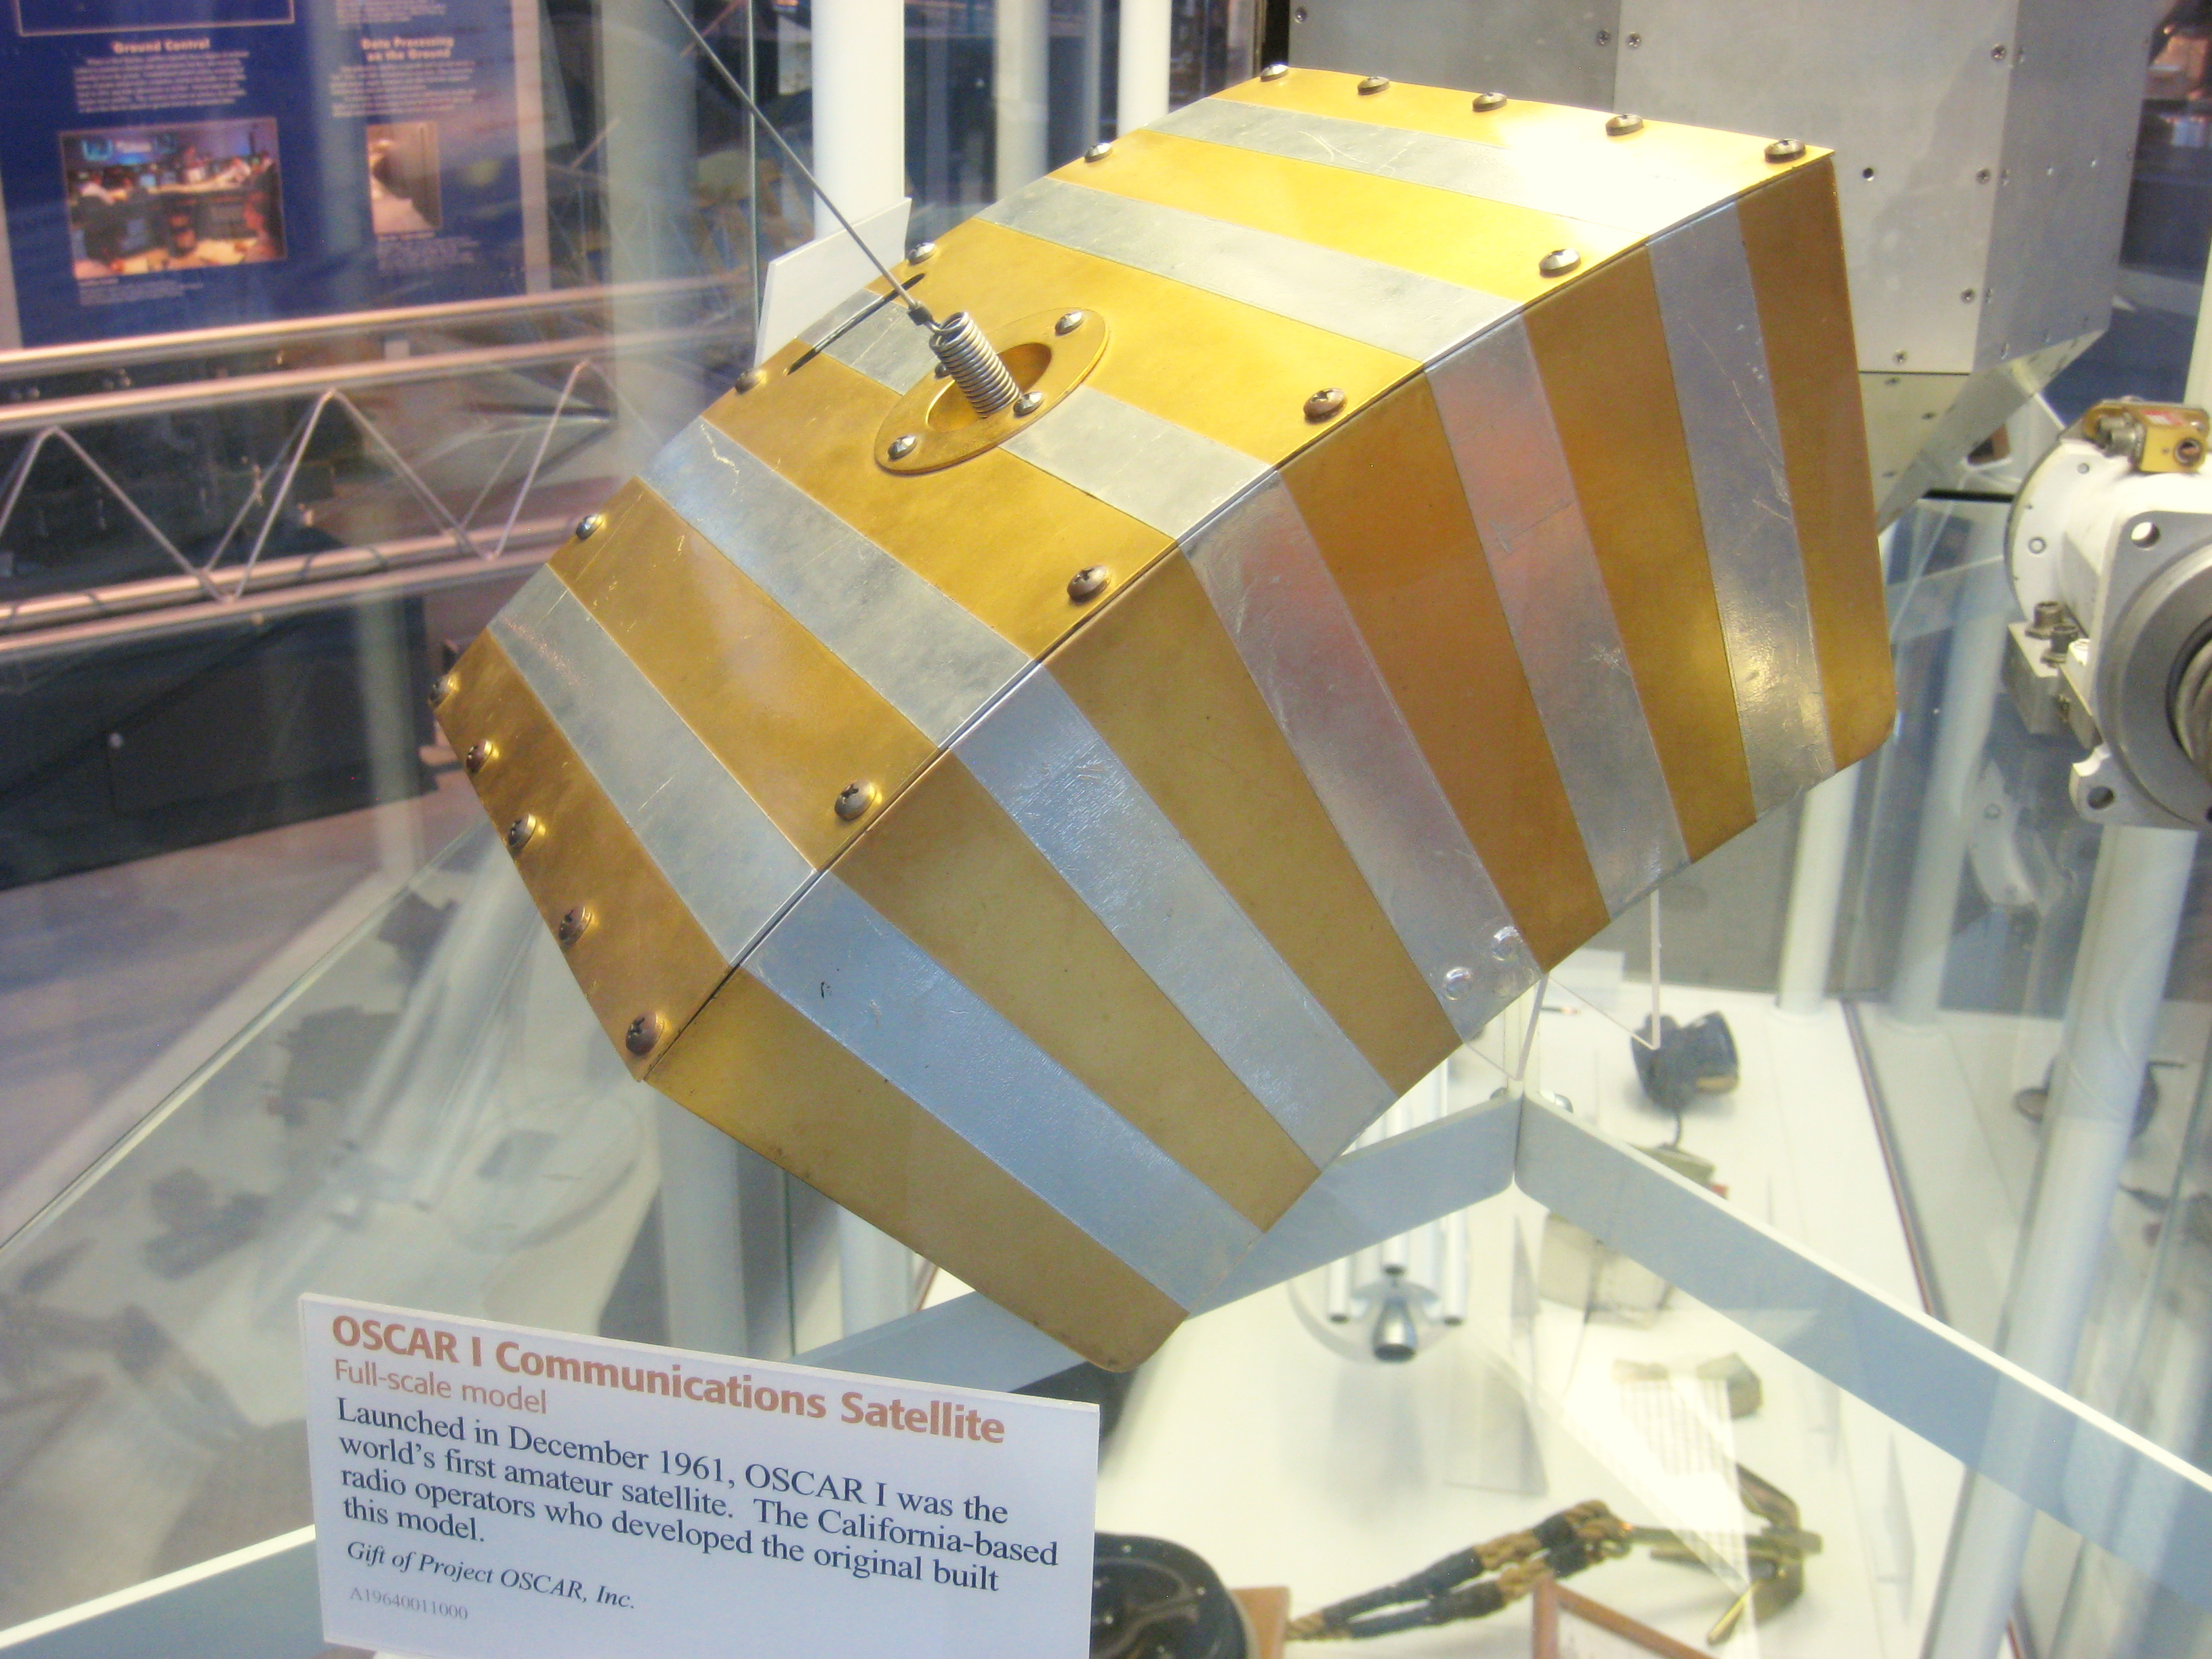
\includegraphics[width=0.85\textwidth]{foto/124}
    \caption{\scriptsize Modell des ersten Amateurfunksatelliten OSCAR 1, der 1961 für 22 Tage aus dem Orbit der Erde eine Bake im \qty{2}{\metre}-Band sendete und von 570 Funkamateuren aus 28 Ländern gehört wurde}
    \label{n_satellit_oscar1}
\end{figure}

    \end{column}
   \begin{column}{0.48\textwidth}
       \begin{itemize}
  \item Umrunden die Erde in kreis- oder elliptischen Bahnen und in unterschiedlichen Höhen
  \item Erster Amateurfunksatellit bereits 1961 (OSCAR 1)
  \item OSCAR: \enquote{Orbiting Satellite Carrying Amateur Radio}
  \item Bis heute mehrere 100 Satelliten im Orbit (gewesen)
  \end{itemize}

   \end{column}
\end{columns}

\end{frame}

\begin{frame}
\only<1>{
\begin{QQuestion}{BE415}{Wofür steht die Abkürzung OSCAR im Amateurfunk?}{Fahrzeug mit betriebsbereiter Amateurfunkstelle (Operational Station on a CAR)}
{Schiff auf See mit Amateurfunkstelle (Offshore Ship Carrying Amateur Radio)}
{Satellit mit Amateurfunkstelle (Orbiting Satellite Carrying Amateur Radio)}
{Amateurfunkstelle im Luftradarbetrieb (Observation Station Conducting Aeronautical Radar)}
\end{QQuestion}

}
\only<2>{
\begin{QQuestion}{BE415}{Wofür steht die Abkürzung OSCAR im Amateurfunk?}{Fahrzeug mit betriebsbereiter Amateurfunkstelle (Operational Station on a CAR)}
{Schiff auf See mit Amateurfunkstelle (Offshore Ship Carrying Amateur Radio)}
{\textbf{\textcolor{DARCgreen}{Satellit mit Amateurfunkstelle (Orbiting Satellite Carrying Amateur Radio)}}}
{Amateurfunkstelle im Luftradarbetrieb (Observation Station Conducting Aeronautical Radar)}
\end{QQuestion}

}
\end{frame}

\begin{frame}
\frametitle{Transponder}
Relaisfunkstelle auf dem Satellit wird \enquote{Transponder} genannt
\begin{columns}
    \begin{column}{0.48\textwidth}
    Uplink: Funkstrecke von der Erde zum Satelliten


    \end{column}
   \begin{column}{0.48\textwidth}
       Downlink: Funkstrecke vom Satelliten zur Erde


   \end{column}
\end{columns}

\begin{itemize}
  \item Unterschiedliche Frequenzbänder für Up- und Downlink
  \item Einfachere Trennung von Sende- und Empfangssignal
  \item Baugröße von Filtern wird reduziert
  \end{itemize}

\end{frame}

\begin{frame}
\only<1>{
\begin{QQuestion}{BE416}{Was versteht man unter dem Transponder eines \glqq OSCAR\grqq{} und wie arbeitet er?}{Dies ist ein Umsetzer an Bord eines Amateurfunksatelliten, der die aufgenommenen Signale in einen anderen Frequenzbereich umsetzt und wieder zur Erde sendet.}
{Es handelt sich um einen mit einer fernbedienten Amateurfunkstelle bestückten Stratosphärenballon, der empfangene Signale aufbereitet zur Erde zurücksendet.}
{Dies ist ein Umsetzer an Bord eines Amateurfunksatelliten, der die vom Satelliten aufgenommenen Wetterbilder und weitere Telemetriedaten automatisch zur Erde sendet.}
{Dies ist ein Bakensender an Bord eines Amateurfunksatelliten, der zur Beobachtung der Ausbreitungsbedingungen im VHF-, UHF- und SHF-Bereich dient.}
\end{QQuestion}

}
\only<2>{
\begin{QQuestion}{BE416}{Was versteht man unter dem Transponder eines \glqq OSCAR\grqq{} und wie arbeitet er?}{\textbf{\textcolor{DARCgreen}{Dies ist ein Umsetzer an Bord eines Amateurfunksatelliten, der die aufgenommenen Signale in einen anderen Frequenzbereich umsetzt und wieder zur Erde sendet.}}}
{Es handelt sich um einen mit einer fernbedienten Amateurfunkstelle bestückten Stratosphärenballon, der empfangene Signale aufbereitet zur Erde zurücksendet.}
{Dies ist ein Umsetzer an Bord eines Amateurfunksatelliten, der die vom Satelliten aufgenommenen Wetterbilder und weitere Telemetriedaten automatisch zur Erde sendet.}
{Dies ist ein Bakensender an Bord eines Amateurfunksatelliten, der zur Beobachtung der Ausbreitungsbedingungen im VHF-, UHF- und SHF-Bereich dient.}
\end{QQuestion}

}
\end{frame}

\begin{frame}
\only<1>{
\begin{QQuestion}{BE411}{Was bedeutet der Begriff Uplink im Bereich der Satellitenkommunikation?}{Senderichtung vom Satelliten zur Erde}
{Senderichtung von der Erde zum Satelliten}
{Horizontaler Winkel der Antenne}
{Vertikaler Winkel der Antenne}
\end{QQuestion}

}
\only<2>{
\begin{QQuestion}{BE411}{Was bedeutet der Begriff Uplink im Bereich der Satellitenkommunikation?}{Senderichtung vom Satelliten zur Erde}
{\textbf{\textcolor{DARCgreen}{Senderichtung von der Erde zum Satelliten}}}
{Horizontaler Winkel der Antenne}
{Vertikaler Winkel der Antenne}
\end{QQuestion}

}
\end{frame}

\begin{frame}
\only<1>{
\begin{QQuestion}{BE412}{Was bedeutet der Begriff Downlink im Bereich der Satellitenkommunikation?}{Senderichtung vom Satelliten zur Erde}
{Senderichtung von der Erde zum Satelliten}
{Horizontaler Winkel der Antenne}
{Vertikaler Winkel der Antenne}
\end{QQuestion}

}
\only<2>{
\begin{QQuestion}{BE412}{Was bedeutet der Begriff Downlink im Bereich der Satellitenkommunikation?}{\textbf{\textcolor{DARCgreen}{Senderichtung vom Satelliten zur Erde}}}
{Senderichtung von der Erde zum Satelliten}
{Horizontaler Winkel der Antenne}
{Vertikaler Winkel der Antenne}
\end{QQuestion}

}
\end{frame}

\begin{frame}
\only<1>{
\begin{QQuestion}{NF113}{Warum befinden sich bei Satellitenbetrieb Up- und Downlink in der Regel nicht im gleichen Frequenzband? Man benutzt unterschiedliche Frequenzbänder, weil~...}{der Uplink durch die Ionosphäre stärker bedämpft wird als der Downlink.}
{dies eine einfachere Trennung von Sende- und Empfangssignal ermöglicht und die Baugröße von Filtern auf dem Satelliten reduziert wird.}
{die Bandbreite auf beiden Frequenzbändern aufgeteilt wird und Bandbereiche besser ausgenutzt werden können. }
{man damit den Dopplereffekt vermindert.}
\end{QQuestion}

}
\only<2>{
\begin{QQuestion}{NF113}{Warum befinden sich bei Satellitenbetrieb Up- und Downlink in der Regel nicht im gleichen Frequenzband? Man benutzt unterschiedliche Frequenzbänder, weil~...}{der Uplink durch die Ionosphäre stärker bedämpft wird als der Downlink.}
{\textbf{\textcolor{DARCgreen}{dies eine einfachere Trennung von Sende- und Empfangssignal ermöglicht und die Baugröße von Filtern auf dem Satelliten reduziert wird.}}}
{die Bandbreite auf beiden Frequenzbändern aufgeteilt wird und Bandbereiche besser ausgenutzt werden können. }
{man damit den Dopplereffekt vermindert.}
\end{QQuestion}

}
\end{frame}

\begin{frame}
\frametitle{Azimut und Elevation}
Satellitenantennen müssen ausgerichtet sein
\begin{columns}
    \begin{column}{0.48\textwidth}
    Azimut

\begin{itemize}
  \item stammt von arabisch السموت (as-sumūt, \enquote{die Wege})
  \item Richtung entlang des Horizonts
  \item Wird wie beim Kompass in Grad gemessen
  \item \qty{0}{\degree}/\qty{360}{\degree} Norden – \qty{90}{\degree} Osten – \qty{180}{\degree} Süden – \qty{270}{\degree} Westen
  \end{itemize}

    \end{column}
   \begin{column}{0.48\textwidth}
       Elevation

\begin{itemize}
  \item leitet sich von lateinisch elevare (\enquote{erheben}) ab
  \item Vertikaler Winkel über dem Horizont
  \item \qty{0}{\degree} $\rightarrow$ direkt am Horizont
  \item \qty{90}{\degree} $\rightarrow$ senkrecht über einem
  \end{itemize}

   \end{column}
\end{columns}

\end{frame}

\begin{frame}
\only<1>{
\begin{QQuestion}{BE413}{Was bedeutet der Begriff Azimut im Bereich der Satellitenkommunikation?}{Vertikaler Winkel der Antenne}
{Horizontaler Winkel der Antenne}
{Senderichtung vom Satelliten zur Erde}
{Senderichtung von der Erde zum Satelliten}
\end{QQuestion}

}
\only<2>{
\begin{QQuestion}{BE413}{Was bedeutet der Begriff Azimut im Bereich der Satellitenkommunikation?}{Vertikaler Winkel der Antenne}
{\textbf{\textcolor{DARCgreen}{Horizontaler Winkel der Antenne}}}
{Senderichtung vom Satelliten zur Erde}
{Senderichtung von der Erde zum Satelliten}
\end{QQuestion}

}
\end{frame}

\begin{frame}
\only<1>{
\begin{QQuestion}{BE414}{Was bedeutet der Begriff Elevation im Bereich der Satellitenkommunikation?}{Horizontaler Winkel der Antenne}
{Vertikaler Winkel der Antenne}
{Senderichtung vom Satelliten zur Erde}
{Senderichtung von der Erde zum Satelliten}
\end{QQuestion}

}
\only<2>{
\begin{QQuestion}{BE414}{Was bedeutet der Begriff Elevation im Bereich der Satellitenkommunikation?}{Horizontaler Winkel der Antenne}
{\textbf{\textcolor{DARCgreen}{Vertikaler Winkel der Antenne}}}
{Senderichtung vom Satelliten zur Erde}
{Senderichtung von der Erde zum Satelliten}
\end{QQuestion}

}
\end{frame}

\begin{frame}
\frametitle{Steuersignale}
\begin{itemize}
  \item Im Amateurfunkdienst gibt es eine Pflicht zur offenen Sprache
  \item Ausnahme: Steuersignale zwischen Bodenstationen und Amateurfunksatelliten
  \item Dürfen zum Zwecke der Verschleierung verschlüsselt werden
  \item Damit können Dritte die Signale nicht mitlesen
  \item Dient der Sicherheit der Satelliten vor Steuerkommandos von Unbefugten
  \item In Deutschland gilt das auch für automatische und fernbediente Stationen sowie Remote-Stationen
  \end{itemize}
\end{frame}

\begin{frame}
\only<1>{
\begin{QQuestion}{VA303}{Welche Kommunikationsinhalte dürfen im internationalen Amateurfunkverkehr laut Radio Regulations (RR) zum Zwecke der Verschleierung verschlüsselt werden?}{Vertrauliche Informationen und Mitteilungen persönlicher Art}
{Steuersignale zwischen Bodenkontrollstationen auf der Erde und Amateurfunksatelliten}
{Inhalte, die auf Grund des verwendeten Übertragungsverfahrens digital codiert werden}
{Inhalte, die schützenswerte technische Sachverhalte des Amateurfunkdienstes betreffen}
\end{QQuestion}

}
\only<2>{
\begin{QQuestion}{VA303}{Welche Kommunikationsinhalte dürfen im internationalen Amateurfunkverkehr laut Radio Regulations (RR) zum Zwecke der Verschleierung verschlüsselt werden?}{Vertrauliche Informationen und Mitteilungen persönlicher Art}
{\textbf{\textcolor{DARCgreen}{Steuersignale zwischen Bodenkontrollstationen auf der Erde und Amateurfunksatelliten}}}
{Inhalte, die auf Grund des verwendeten Übertragungsverfahrens digital codiert werden}
{Inhalte, die schützenswerte technische Sachverhalte des Amateurfunkdienstes betreffen}
\end{QQuestion}

}
\end{frame}

\begin{frame}
\only<1>{
\begin{QQuestion}{VD104}{Welche Kommunikationsinhalte dürfen im Amateurfunkverkehr laut AFuV zum Zwecke der Verschleierung verschlüsselt werden?}{Inhalte, die auf Grund des verwendeten Übertragungsverfahrens digital codiert werden}
{Steuersignale für Satelliten, vertrauliche Informationen und Mitteilung persönlicher Art}
{Steuersignale für Satelliten, für fernbediente und automatisch arbeitende Stationen und für Remote-Betrieb}
{Inhalte, die schützenswerte technische Sachverhalte des Amateurfunkdienstes betreffen}
\end{QQuestion}

}
\only<2>{
\begin{QQuestion}{VD104}{Welche Kommunikationsinhalte dürfen im Amateurfunkverkehr laut AFuV zum Zwecke der Verschleierung verschlüsselt werden?}{Inhalte, die auf Grund des verwendeten Übertragungsverfahrens digital codiert werden}
{Steuersignale für Satelliten, vertrauliche Informationen und Mitteilung persönlicher Art}
{\textbf{\textcolor{DARCgreen}{Steuersignale für Satelliten, für fernbediente und automatisch arbeitende Stationen und für Remote-Betrieb}}}
{Inhalte, die schützenswerte technische Sachverhalte des Amateurfunkdienstes betreffen}
\end{QQuestion}

}
\end{frame}%ENDCONTENT


\section{Exterritoriale Stationen}
\label{section:exterritoriale_stationen}
\begin{frame}%STARTCONTENT

\begin{columns}
    \begin{column}{0.48\textwidth}
    \begin{itemize}
  \item Amateurfunkstelle außerhalb des Hoheitsgebiets der BRD
  \item Und kein anderes Land hat an diesem Standort ein Hoheitsgebiet
  \item Rufzeichen aus dem Block DP0AA bis DP2ZZ
  \end{itemize}

    \end{column}
   \begin{column}{0.48\textwidth}
       
\begin{figure}
    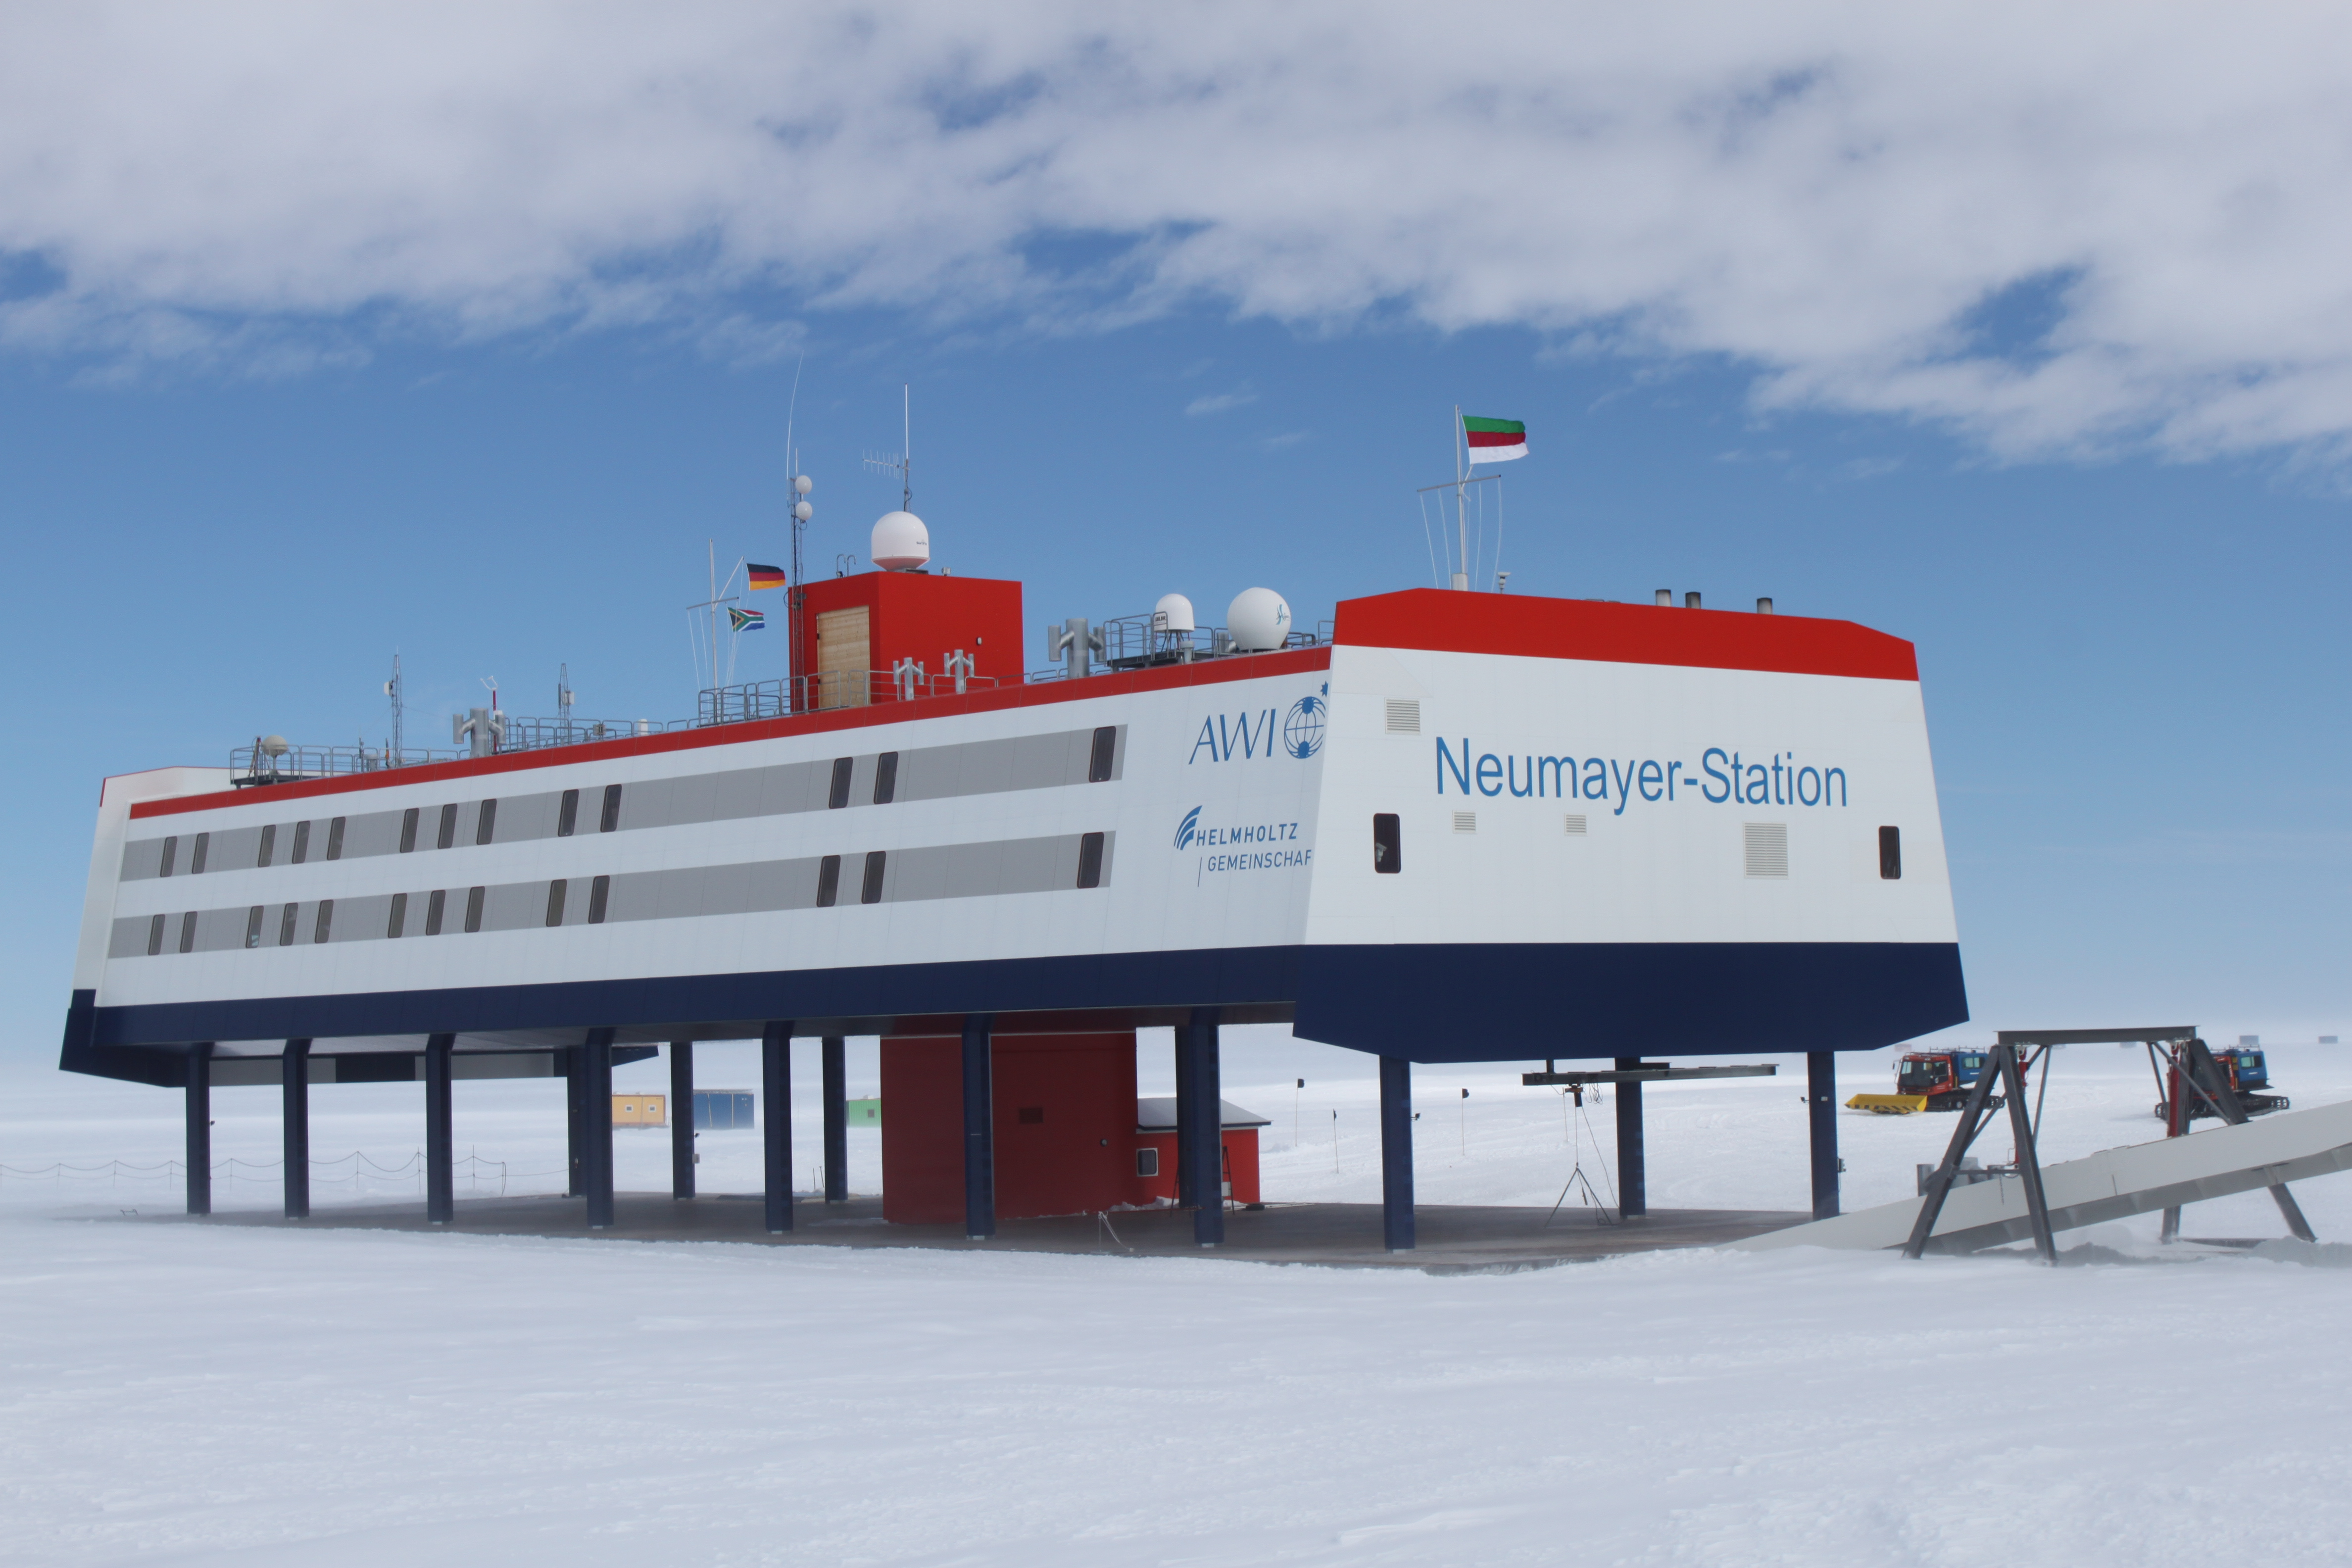
\includegraphics[width=0.85\textwidth]{foto/126}
    \caption{\scriptsize Auf der Polarforschungsstation Neumayer III befindet sich die Amateurfunkstation DP0GVN.}
    \label{n_exterritoriale_stationen_neumeyer_station}
\end{figure}

   \end{column}
\end{columns}

\end{frame}

\begin{frame}
\begin{columns}
    \begin{column}{0.48\textwidth}
    Beispiele:

\begin{itemize}
  \item Internationale Raumstation (ISS): DP0ISS
  \item Neumayer~III-Forschungsstation in der Antarktis: DP0GVN
  \item Forschungsschiff Polarstern: DP0POL
  \end{itemize}

    \end{column}
   \begin{column}{0.48\textwidth}
       
\begin{figure}
    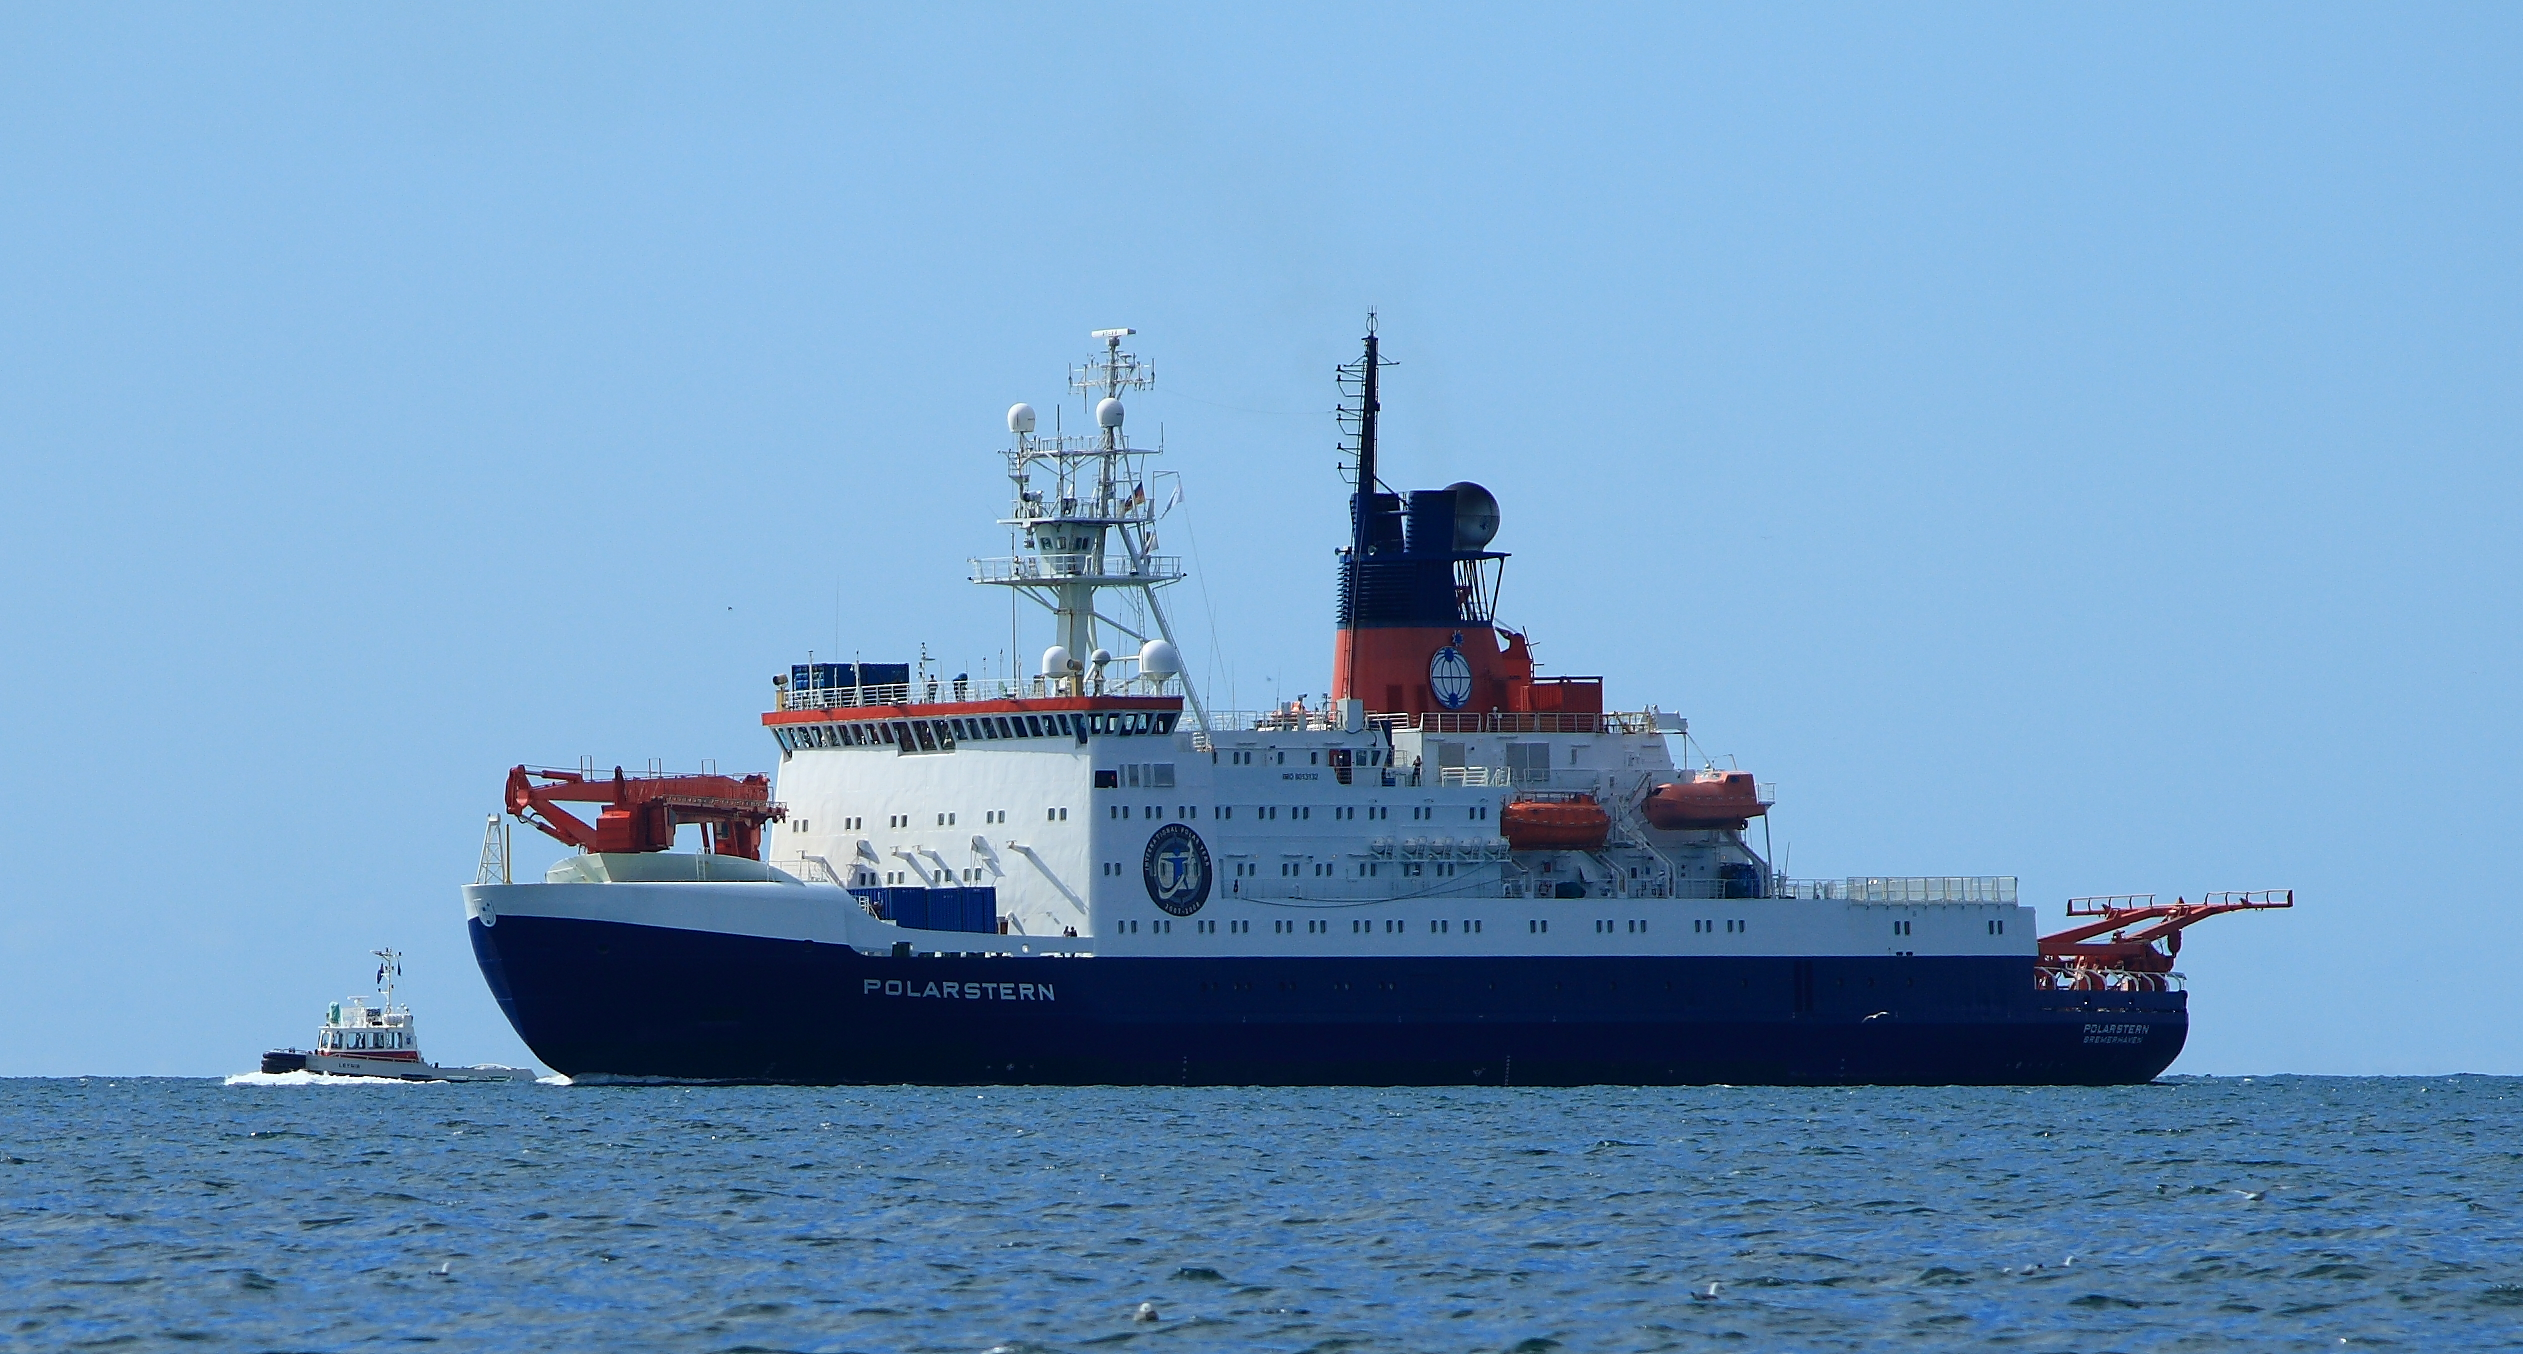
\includegraphics[width=0.85\textwidth]{foto/125}
    \caption{\scriptsize Die Amateurfunkstation an Bord des Forschungsschiff Polarstern verwendet das Rufzeichen DP0POL.}
    \label{n_exterritoriale_stationen_polarstern}
\end{figure}

   \end{column}
\end{columns}

\end{frame}

\begin{frame}
\only<1>{
\begin{QQuestion}{BD107}{Sie hören die Station DP0GVN. Um welche Art von Amateurfunkstelle handelt es sich? Es handelt sich um eine~...}{Amateurfunkstelle der Klasse A, die exterritorial betrieben wird.}
{Amateurfunkstelle der Klasse E, die ohne Anzeige nach BEMFV betrieben werden darf.}
{Klubstation der Klasse A von Funkamateuren, die Angehörige der Gaststreitkräfte in Deutschland sind.}
{Amateurfunkstelle der Klasse E, die exterritorial betrieben wird.}
\end{QQuestion}

}
\only<2>{
\begin{QQuestion}{BD107}{Sie hören die Station DP0GVN. Um welche Art von Amateurfunkstelle handelt es sich? Es handelt sich um eine~...}{\textbf{\textcolor{DARCgreen}{Amateurfunkstelle der Klasse A, die exterritorial betrieben wird.}}}
{Amateurfunkstelle der Klasse E, die ohne Anzeige nach BEMFV betrieben werden darf.}
{Klubstation der Klasse A von Funkamateuren, die Angehörige der Gaststreitkräfte in Deutschland sind.}
{Amateurfunkstelle der Klasse E, die exterritorial betrieben wird.}
\end{QQuestion}

}
\end{frame}

\begin{frame}
\only<1>{
\begin{QQuestion}{BD108}{Sie hören die Station DP0POL. Um welche Art von Amateurfunkstelle handelt es sich? Es handelt sich um eine Amateurfunkstelle~...}{von Angehörigen der Gaststreitkräfte in Deutschland.}
{der Klasse E, die ohne Anzeige nach BEMFV betrieben werden darf.}
{eines ausländischen Funkamateurs, der eine Amateurfunkprüfungsbescheinigung, aber kein individuelles Rufzeichen hat.}
{der Klasse A, die an einem exterritorialen Standort betrieben wird.}
\end{QQuestion}

}
\only<2>{
\begin{QQuestion}{BD108}{Sie hören die Station DP0POL. Um welche Art von Amateurfunkstelle handelt es sich? Es handelt sich um eine Amateurfunkstelle~...}{von Angehörigen der Gaststreitkräfte in Deutschland.}
{der Klasse E, die ohne Anzeige nach BEMFV betrieben werden darf.}
{eines ausländischen Funkamateurs, der eine Amateurfunkprüfungsbescheinigung, aber kein individuelles Rufzeichen hat.}
{\textbf{\textcolor{DARCgreen}{der Klasse A, die an einem exterritorialen Standort betrieben wird.}}}
\end{QQuestion}

}
\end{frame}%ENDCONTENT


\section{Experimentelle Studien}
\label{section:experimentelle_studien}
\begin{frame}%STARTCONTENT
\begin{itemize}
  \item Für besondere experimentelle und technisch-wissenschaftliche Studien
  \item Zeitlich und im Berechtigungsumfang eingeschränkt
  \item Werden gemäß §~16 Absatz 2 Satz 2 AFuV betrieben
  \item Klasse~A: DA5AA bis DA5ZZZ
  \item Klasse~E: DA4AA bis DA4ZZZ
  \item Bei der BNetzA zu beantragen
  \end{itemize}
\end{frame}

\begin{frame}
\only<1>{
\begin{QQuestion}{BD102}{Sie hören die Station DA5XX. Um welche Art von Amateurfunkstelle handelt es sich? Es handelt sich um eine~...}{Kurzzeitzuteilung für einen ausländischen Funkamateur, der eine Amateurfunkprüfungsbescheinigung, aber kein individuelles Rufzeichen hat.}
{Versuchsfunkstelle, die zur Erprobung technischer oder wissenschaftlicher Entwicklungen betrieben wird.}
{exterritoriale deutsche Funkstelle des Amateurfunkdienstes oder des Amateurfunkdienstes über Satelliten.}
{Amateurfunkstelle, die für besondere experimentelle Studien gemäß § 16 Absatz 2 AFuV betrieben wird.}
\end{QQuestion}

}
\only<2>{
\begin{QQuestion}{BD102}{Sie hören die Station DA5XX. Um welche Art von Amateurfunkstelle handelt es sich? Es handelt sich um eine~...}{Kurzzeitzuteilung für einen ausländischen Funkamateur, der eine Amateurfunkprüfungsbescheinigung, aber kein individuelles Rufzeichen hat.}
{Versuchsfunkstelle, die zur Erprobung technischer oder wissenschaftlicher Entwicklungen betrieben wird.}
{exterritoriale deutsche Funkstelle des Amateurfunkdienstes oder des Amateurfunkdienstes über Satelliten.}
{\textbf{\textcolor{DARCgreen}{Amateurfunkstelle, die für besondere experimentelle Studien gemäß § 16 Absatz 2 AFuV betrieben wird.}}}
\end{QQuestion}

}
\end{frame}

\begin{frame}
\only<1>{
\begin{QQuestion}{VD116}{Für welche Zwecke sind Zuteilungen mit Ausnahmen von den technischen und betrieblichen Rahmenbedingungen der Amateurfunkverordnung (AFuV) möglich?}{Für Abgleicharbeiten und Messungen an Sendern ohne Abschlusswiderstand}
{Für Übungen zur Abwicklung des Funkverkehrs in Not- und Katastrophenfällen}
{Für besondere experimentelle und technisch-wissenschaftliche Studien mit einer Amateurfunkstelle}
{Für die Nutzung zusätzlicher Frequenzbereiche, die nicht im Frequenznutzungsplan für den Amateurfunkdienst ausgewiesen sind}
\end{QQuestion}

}
\only<2>{
\begin{QQuestion}{VD116}{Für welche Zwecke sind Zuteilungen mit Ausnahmen von den technischen und betrieblichen Rahmenbedingungen der Amateurfunkverordnung (AFuV) möglich?}{Für Abgleicharbeiten und Messungen an Sendern ohne Abschlusswiderstand}
{Für Übungen zur Abwicklung des Funkverkehrs in Not- und Katastrophenfällen}
{\textbf{\textcolor{DARCgreen}{Für besondere experimentelle und technisch-wissenschaftliche Studien mit einer Amateurfunkstelle}}}
{Für die Nutzung zusätzlicher Frequenzbereiche, die nicht im Frequenznutzungsplan für den Amateurfunkdienst ausgewiesen sind}
\end{QQuestion}

}
\end{frame}%ENDCONTENT


\title{DARC Amateurfunklehrgang Klasse N}
\author{Internationaler Funkbetrieb}
\institute{Deutscher Amateur Radio Club e.\,V.}
\begin{frame}
\maketitle
\end{frame}

\section{Internationale Landeskenner}
\label{section:internationale_landeskenner}
\begin{frame}%STARTCONTENT

\begin{columns}
    \begin{column}{0.48\textwidth}
    \begin{itemize}
  \item Anhand des Präfixes kann man erkennen, aus welchem Land ein Funkpartner kommt
  \item Blau markierte Länder kommen im Fragenkatalog vor
  \end{itemize}

    \end{column}
   \begin{column}{0.48\textwidth}
       
\begin{figure}
    \DARCimage{0.85\linewidth}{656include}
    \caption{\scriptsize Landeskenner in Europa}
    \label{n_internationale_landeskenner_eu}
\end{figure}


   \end{column}
\end{columns}

\end{frame}

\begin{frame}
\only<1>{
\begin{QQuestion}{BD301}{Wo können Sie nachschlagen, in welchem Land sich eine Amateurfunkstelle mit einem Ihnen bislang unbekannten Landeskenner befindet?}{In den Empfehlungen der IARU.}
{In der Rufzeichenliste der Bundesnetzagentur.}
{In der Landeskennerliste der ITU, Amateurfunkhandbüchern und Rufzeichenlisten.}
{Im Frequenzbereichszuweisungsplan der Bundesrepublik Deutschland.}
\end{QQuestion}

}
\only<2>{
\begin{QQuestion}{BD301}{Wo können Sie nachschlagen, in welchem Land sich eine Amateurfunkstelle mit einem Ihnen bislang unbekannten Landeskenner befindet?}{In den Empfehlungen der IARU.}
{In der Rufzeichenliste der Bundesnetzagentur.}
{\textbf{\textcolor{DARCgreen}{In der Landeskennerliste der ITU, Amateurfunkhandbüchern und Rufzeichenlisten.}}}
{Im Frequenzbereichszuweisungsplan der Bundesrepublik Deutschland.}
\end{QQuestion}

}
\end{frame}

\begin{frame}
\only<1>{
\begin{QQuestion}{BD314}{Welche Antwort enthält nur Landeskenner von Ländern, die an die Bundesrepublik Deutschland grenzen?}{SM, LA, LZ, HB0}
{EA, GM, OE, ON}
{F, HB9, OZ, SP}
{CT, I, LX, OK}
\end{QQuestion}

}
\only<2>{
\begin{QQuestion}{BD314}{Welche Antwort enthält nur Landeskenner von Ländern, die an die Bundesrepublik Deutschland grenzen?}{SM, LA, LZ, HB0}
{EA, GM, OE, ON}
{\textbf{\textcolor{DARCgreen}{F, HB9, OZ, SP}}}
{CT, I, LX, OK}
\end{QQuestion}

}
\end{frame}

\begin{frame}
\only<1>{
\begin{QQuestion}{BD311}{Welche Gruppe gibt die Landeskenner der Länder Spanien, Luxemburg und Polen für ihre Amateurfunkstellen richtig wieder?}{EI, LA, SM}
{EU, LZ, S0}
{EA, LX, SP}
{EM, LU, 4X}
\end{QQuestion}

}
\only<2>{
\begin{QQuestion}{BD311}{Welche Gruppe gibt die Landeskenner der Länder Spanien, Luxemburg und Polen für ihre Amateurfunkstellen richtig wieder?}{EI, LA, SM}
{EU, LZ, S0}
{\textbf{\textcolor{DARCgreen}{EA, LX, SP}}}
{EM, LU, 4X}
\end{QQuestion}

}
\end{frame}

\begin{frame}
\only<1>{
\begin{QQuestion}{BD304}{Welche Landeskenner sind der Reihe nach den folgenden Ländern zugeordnet? Die Landeskenner OE, PA, und SM entsprechen den Ländern~...}{Österreich, Niederlande und Schweden.}
{Österreich, Brasilien und Schweiz.}
{Österreich, Polen und Südafrika.}
{Österreich, Niederlande und Schottland.}
\end{QQuestion}

}
\only<2>{
\begin{QQuestion}{BD304}{Welche Landeskenner sind der Reihe nach den folgenden Ländern zugeordnet? Die Landeskenner OE, PA, und SM entsprechen den Ländern~...}{\textbf{\textcolor{DARCgreen}{Österreich, Niederlande und Schweden.}}}
{Österreich, Brasilien und Schweiz.}
{Österreich, Polen und Südafrika.}
{Österreich, Niederlande und Schottland.}
\end{QQuestion}

}
\end{frame}

\begin{frame}
\only<1>{
\begin{QQuestion}{BD307}{Welche Länder (Gebiete) sind der Reihe nach den folgenden Landeskennern zugeordnet? Die Landeskenner 4X, F und OZ entsprechen den Ländern (Gebieten)~...}{Israel, Frankreich und Dänemark.}
{Italien, Belgien und Slowakei.}
{Schweden, Belgien und Schottland.}
{Schweiz, Luxemburg und Polen.}
\end{QQuestion}

}
\only<2>{
\begin{QQuestion}{BD307}{Welche Länder (Gebiete) sind der Reihe nach den folgenden Landeskennern zugeordnet? Die Landeskenner 4X, F und OZ entsprechen den Ländern (Gebieten)~...}{\textbf{\textcolor{DARCgreen}{Israel, Frankreich und Dänemark.}}}
{Italien, Belgien und Slowakei.}
{Schweden, Belgien und Schottland.}
{Schweiz, Luxemburg und Polen.}
\end{QQuestion}

}
\end{frame}

\begin{frame}
\only<1>{
\begin{QQuestion}{BD303}{Welche Länder sind der Reihe nach den folgenden Landeskennern zugeordnet? Die Landeskenner OE, ON und OK entsprechen den Ländern~...}{Finnland, Tschechien und Dänemark.}
{Dänemark, Belgien und Slowakei.}
{Österreich, Dänemark und Belgien.}
{Österreich, Belgien und Tschechien.}
\end{QQuestion}

}
\only<2>{
\begin{QQuestion}{BD303}{Welche Länder sind der Reihe nach den folgenden Landeskennern zugeordnet? Die Landeskenner OE, ON und OK entsprechen den Ländern~...}{Finnland, Tschechien und Dänemark.}
{Dänemark, Belgien und Slowakei.}
{Österreich, Dänemark und Belgien.}
{\textbf{\textcolor{DARCgreen}{Österreich, Belgien und Tschechien.}}}
\end{QQuestion}

}
\end{frame}

\begin{frame}
\only<1>{
\begin{QQuestion}{BD305}{Welche Länder sind der Reihe nach den folgenden Landeskennern zugeordnet? Die Landeskenner F, PA und SP entsprechen den Ländern~...}{Frankreich, Niederlande und Polen.}
{Schweden, Niederlande und Polen.}
{Niederlande, Polen und Belgien.}
{Südafrika, Dänemark und Luxemburg.}
\end{QQuestion}

}
\only<2>{
\begin{QQuestion}{BD305}{Welche Länder sind der Reihe nach den folgenden Landeskennern zugeordnet? Die Landeskenner F, PA und SP entsprechen den Ländern~...}{\textbf{\textcolor{DARCgreen}{Frankreich, Niederlande und Polen.}}}
{Schweden, Niederlande und Polen.}
{Niederlande, Polen und Belgien.}
{Südafrika, Dänemark und Luxemburg.}
\end{QQuestion}

}
\end{frame}

\begin{frame}
\only<1>{
\begin{QQuestion}{BD306}{Welche Länder sind der Reihe nach den folgenden Landeskennern zugeordnet? Die Landeskenner SM, SP und ZS entsprechen den Ländern~...}{Schweden, Slowenien und Polen.}
{Schweden, Slowakei und Polen.}
{Slowenien, Polen und Schweden.}
{Schweden, Polen und Südafrika.}
\end{QQuestion}

}
\only<2>{
\begin{QQuestion}{BD306}{Welche Länder sind der Reihe nach den folgenden Landeskennern zugeordnet? Die Landeskenner SM, SP und ZS entsprechen den Ländern~...}{Schweden, Slowenien und Polen.}
{Schweden, Slowakei und Polen.}
{Slowenien, Polen und Schweden.}
{\textbf{\textcolor{DARCgreen}{Schweden, Polen und Südafrika.}}}
\end{QQuestion}

}
\end{frame}

\begin{frame}
\only<1>{
\begin{QQuestion}{BD308}{Welche Länder sind der Reihe nach den folgenden Landeskennern zugeordnet? Die Landeskenner EA, EI, EK, EM, ES entsprechen den Ländern~...}{Spanien, Ukraine, Armenien, Estland, Irland}
{Spanien, Ukraine, Armenien, Irland, Estland}
{Spanien, Irland, Armenien, Estland, Ukraine}
{Spanien, Irland, Armenien, Ukraine, Estland}
\end{QQuestion}

}
\only<2>{
\begin{QQuestion}{BD308}{Welche Länder sind der Reihe nach den folgenden Landeskennern zugeordnet? Die Landeskenner EA, EI, EK, EM, ES entsprechen den Ländern~...}{Spanien, Ukraine, Armenien, Estland, Irland}
{Spanien, Ukraine, Armenien, Irland, Estland}
{Spanien, Irland, Armenien, Estland, Ukraine}
{\textbf{\textcolor{DARCgreen}{Spanien, Irland, Armenien, Ukraine, Estland}}}
\end{QQuestion}

}
\end{frame}

\begin{frame}
\only<1>{
\begin{QQuestion}{BD310}{Welche Gruppe gibt die Landeskenner der Länder Schweiz, Spanien und Belgien für ihre Amateurfunkstellen richtig wieder?}{SZ, SP und BE}
{HB9, EA und ON}
{SP, ON und EA}
{EA, SP und BE}
\end{QQuestion}

}
\only<2>{
\begin{QQuestion}{BD310}{Welche Gruppe gibt die Landeskenner der Länder Schweiz, Spanien und Belgien für ihre Amateurfunkstellen richtig wieder?}{SZ, SP und BE}
{\textbf{\textcolor{DARCgreen}{HB9, EA und ON}}}
{SP, ON und EA}
{EA, SP und BE}
\end{QQuestion}

}
\end{frame}

\begin{frame}
\only<1>{
\begin{QQuestion}{BD302}{Welchem Land bzw. welchen Ländern sind die Landeskenner DA bis DZ zugeordnet?}{Deutschland (DA-DO), Taiwan (DP-DT) und Philippinen (DU-DZ)}
{Ausschließlich Deutschland (DA-DZ)}
{Deutschland (DA-DT) und Philippinen (DU-DZ)}
{Deutschland (DA-DR), Südkorea (DS-DT) und Philippinen (DU-DZ)}
\end{QQuestion}

}
\only<2>{
\begin{QQuestion}{BD302}{Welchem Land bzw. welchen Ländern sind die Landeskenner DA bis DZ zugeordnet?}{Deutschland (DA-DO), Taiwan (DP-DT) und Philippinen (DU-DZ)}
{Ausschließlich Deutschland (DA-DZ)}
{Deutschland (DA-DT) und Philippinen (DU-DZ)}
{\textbf{\textcolor{DARCgreen}{Deutschland (DA-DR), Südkorea (DS-DT) und Philippinen (DU-DZ)}}}
\end{QQuestion}

}
\end{frame}

\begin{frame}
\only<1>{
\begin{QQuestion}{BD312}{Welche Gruppe gibt Landeskenner der Länder USA, Neuseeland und Argentinien für ihre Amateurfunkstellen richtig wieder?}{AL, CE und VE}
{K, ZS und A}
{N, LU und PY}
{W, ZL und LU}
\end{QQuestion}

}
\only<2>{
\begin{QQuestion}{BD312}{Welche Gruppe gibt Landeskenner der Länder USA, Neuseeland und Argentinien für ihre Amateurfunkstellen richtig wieder?}{AL, CE und VE}
{K, ZS und A}
{N, LU und PY}
{\textbf{\textcolor{DARCgreen}{W, ZL und LU}}}
\end{QQuestion}

}
\end{frame}

\begin{frame}
\only<1>{
\begin{QQuestion}{BD313}{Welche Gruppe gibt Landeskenner der Länder China, Kanada und Australien für ihre Amateurfunkstellen richtig wieder?}{JA, VE und VK}
{BY, JA und VK}
{BY, VE und VK}
{N, VE und VK}
\end{QQuestion}

}
\only<2>{
\begin{QQuestion}{BD313}{Welche Gruppe gibt Landeskenner der Länder China, Kanada und Australien für ihre Amateurfunkstellen richtig wieder?}{JA, VE und VK}
{BY, JA und VK}
{\textbf{\textcolor{DARCgreen}{BY, VE und VK}}}
{N, VE und VK}
\end{QQuestion}

}
\end{frame}

\begin{frame}
\only<1>{
\begin{QQuestion}{BD316}{Welche drei Landeskenner sind einem einzigen Kontinent zuzuordnen?}{N, XE und DS}
{K, VE und BY}
{W, VE und XE}
{XE, VE und JA}
\end{QQuestion}

}
\only<2>{
\begin{QQuestion}{BD316}{Welche drei Landeskenner sind einem einzigen Kontinent zuzuordnen?}{N, XE und DS}
{K, VE und BY}
{\textbf{\textcolor{DARCgreen}{W, VE und XE}}}
{XE, VE und JA}
\end{QQuestion}

}
\end{frame}

\begin{frame}
\only<1>{
\begin{QQuestion}{BD318}{Welche Landeskenner sind asiatischen Ländern zugewiesen?}{JA, VU und PY}
{VU, JA und K}
{BY, JA und VU}
{LU, DS und JA}
\end{QQuestion}

}
\only<2>{
\begin{QQuestion}{BD318}{Welche Landeskenner sind asiatischen Ländern zugewiesen?}{JA, VU und PY}
{VU, JA und K}
{\textbf{\textcolor{DARCgreen}{BY, JA und VU}}}
{LU, DS und JA}
\end{QQuestion}

}
\end{frame}

\begin{frame}
\only<1>{
\begin{QQuestion}{BD317}{Welche Landeskenner sind südamerikanischen Ländern zugewiesen?}{LU, CE und BY}
{PY, CE und LU}
{CE, LU und JA}
{PY, CE und VE}
\end{QQuestion}

}
\only<2>{
\begin{QQuestion}{BD317}{Welche Landeskenner sind südamerikanischen Ländern zugewiesen?}{LU, CE und BY}
{\textbf{\textcolor{DARCgreen}{PY, CE und LU}}}
{CE, LU und JA}
{PY, CE und VE}
\end{QQuestion}

}
\end{frame}

\begin{frame}
\only<1>{
\begin{QQuestion}{BD309}{Welche Länder sind der Reihe nach den folgenden Landeskennern zugeordnet? Die Landeskenner VE, VK und PY entsprechen den Ländern~...}{Kanada, Australien und Brasilien.}
{Kanada, Brasilien und USA.}
{USA, Australien und Brasilien.}
{Kanada, Australien und Japan.}
\end{QQuestion}

}
\only<2>{
\begin{QQuestion}{BD309}{Welche Länder sind der Reihe nach den folgenden Landeskennern zugeordnet? Die Landeskenner VE, VK und PY entsprechen den Ländern~...}{\textbf{\textcolor{DARCgreen}{Kanada, Australien und Brasilien.}}}
{Kanada, Brasilien und USA.}
{USA, Australien und Brasilien.}
{Kanada, Australien und Japan.}
\end{QQuestion}

}
\end{frame}

\begin{frame}
\only<1>{
\begin{QQuestion}{BD315}{Welche Antwort gibt ausschließlich Rufzeichen aus den Vereinigten Staaten (USA) wieder?}{K1TTT, KA7KLE und UA3RUS}
{W0FKK, N6CAL und VE5VK}
{US2ABC, AB0GC und W4EAX}
{K3LR, W3DZZ und K4EAX}
\end{QQuestion}

}
\only<2>{
\begin{QQuestion}{BD315}{Welche Antwort gibt ausschließlich Rufzeichen aus den Vereinigten Staaten (USA) wieder?}{K1TTT, KA7KLE und UA3RUS}
{W0FKK, N6CAL und VE5VK}
{US2ABC, AB0GC und W4EAX}
{\textbf{\textcolor{DARCgreen}{K3LR, W3DZZ und K4EAX}}}
\end{QQuestion}

}
\end{frame}%ENDCONTENT


\section{ITU-Regionen}
\label{section:itu_regionen}
\begin{frame}%STARTCONTENT

\begin{columns}
    \begin{column}{0.48\textwidth}
    
\begin{figure}
    \DARCimage{0.85\linewidth}{658include}
    \caption{\scriptsize Kartendarstellung der ITU-Regionen}
    \label{n_itu_regionen_karte}
\end{figure}


    \end{column}
   \begin{column}{0.48\textwidth}
       \begin{itemize}
  \item Weltweite Koordinierung von Funkfrequenzen getrennt nach 3 Regionen
  \item Durch ITU geregelt
  \item Nötig, um unterschiedliche Zuweisungen von Frequenzbereichen zu Funkdiensten vorzunehmen
  \end{itemize}

   \end{column}
\end{columns}

\end{frame}

\begin{frame}
\only<1>{
\begin{QQuestion}{VA402}{Nach den Radio Regulations (RR) ist die Welt für die Zuweisung von Frequenzbereichen an Funkdienste in Regionen aufgeteilt. Wie viele Regionen gibt es?}{Zwei}
{Fünf}
{Vier}
{Drei}
\end{QQuestion}

}
\only<2>{
\begin{QQuestion}{VA402}{Nach den Radio Regulations (RR) ist die Welt für die Zuweisung von Frequenzbereichen an Funkdienste in Regionen aufgeteilt. Wie viele Regionen gibt es?}{Zwei}
{Fünf}
{Vier}
{\textbf{\textcolor{DARCgreen}{Drei}}}
\end{QQuestion}

}
\end{frame}

\begin{frame}
\only<1>{
\begin{QQuestion}{VA401}{Weshalb wird in den Radio Regulations (RR) die Erde in verschiedene Regionen eingeteilt?}{Weil es sich um unterschiedliche Zeitzonen handelt und es so den Funkverkehr vereinfacht}
{Weil der Amateurfunkverkehr nur innerhalb einer Region zulässig ist}
{Um für die einzelnen Regionen Regelungen für Gastlizenzen einführen zu können}
{Um in den Regionen unterschiedliche Frequenzbereichszuweisungen für die Funkdienste vornehmen zu können}
\end{QQuestion}

}
\only<2>{
\begin{QQuestion}{VA401}{Weshalb wird in den Radio Regulations (RR) die Erde in verschiedene Regionen eingeteilt?}{Weil es sich um unterschiedliche Zeitzonen handelt und es so den Funkverkehr vereinfacht}
{Weil der Amateurfunkverkehr nur innerhalb einer Region zulässig ist}
{Um für die einzelnen Regionen Regelungen für Gastlizenzen einführen zu können}
{\textbf{\textcolor{DARCgreen}{Um in den Regionen unterschiedliche Frequenzbereichszuweisungen für die Funkdienste vornehmen zu können}}}
\end{QQuestion}

}
\end{frame}

\begin{frame}
\only<1>{
\begin{QQuestion}{VA403}{Zu welcher Region nach den Radio Regulations (RR) gehört Deutschland?}{Region 2}
{Region 1}
{Region 3}
{Region 4}
\end{QQuestion}

}
\only<2>{
\begin{QQuestion}{VA403}{Zu welcher Region nach den Radio Regulations (RR) gehört Deutschland?}{Region 2}
{\textbf{\textcolor{DARCgreen}{Region 1}}}
{Region 3}
{Region 4}
\end{QQuestion}

}
\end{frame}

\begin{frame}
\only<1>{
\begin{QQuestion}{VA404}{Zu welcher Region nach den Radio Regulations (RR) gehört Kanada?}{Region 3}
{Region 2}
{Region 4}
{Region 1}
\end{QQuestion}

}
\only<2>{
\begin{QQuestion}{VA404}{Zu welcher Region nach den Radio Regulations (RR) gehört Kanada?}{Region 3}
{\textbf{\textcolor{DARCgreen}{Region 2}}}
{Region 4}
{Region 1}
\end{QQuestion}

}
\end{frame}

\begin{frame}
\only<1>{
\begin{QQuestion}{VA405}{Zu welcher Region nach den Radio Regulations (RR) gehört Australien?}{Region 3}
{Region 1}
{Region 2}
{Region 4}
\end{QQuestion}

}
\only<2>{
\begin{QQuestion}{VA405}{Zu welcher Region nach den Radio Regulations (RR) gehört Australien?}{\textbf{\textcolor{DARCgreen}{Region 3}}}
{Region 1}
{Region 2}
{Region 4}
\end{QQuestion}

}
\end{frame}%ENDCONTENT


\section{DX}
\label{section:dx}
\begin{frame}%STARTCONTENT
\begin{itemize}
  \item Funkverbindung über große Entfernung
  \item DX $\rightarrow$ \enquote{long distance} (aus Morsetelegrafie)
  \item Unterscheidung zwischen Kurzwelle und UKW
  \end{itemize}
\end{frame}

\begin{frame}
\frametitle{DX Kurzwelle}
\begin{columns}
    \begin{column}{0.48\textwidth}
    \begin{itemize}
  \item Kontakt mit Funkamateuren von einem anderen Kontinent
  \item Funkamateure vom selben Kontinent sollten nicht antworten
  \end{itemize}

    \end{column}
   \begin{column}{0.48\textwidth}
       
    \pause\QSOown{CQ DX}



   \end{column}
\end{columns}

\end{frame}

\begin{frame}
\only<1>{
\begin{QQuestion}{BB103}{Was bedeutet die betriebliche Abkürzung DX?}{Kleine Entfernung }
{Große Entfernung }
{Auf dem indirektem Weg}
{Auf dem direktem Weg}
\end{QQuestion}

}
\only<2>{
\begin{QQuestion}{BB103}{Was bedeutet die betriebliche Abkürzung DX?}{Kleine Entfernung }
{\textbf{\textcolor{DARCgreen}{Große Entfernung }}}
{Auf dem indirektem Weg}
{Auf dem direktem Weg}
\end{QQuestion}

}
\end{frame}

\begin{frame}
\only<1>{
\begin{QQuestion}{BE114}{Was bedeutet der im \qty{20}{\m}-Band gesendete Anruf \glqq CQ DX CQ DX DE HB9AFN HB9AFN K\grqq{}? HB9AFN sucht eine Verbindung mit~...}{einem anderen Kontinent und sollte durch europäische Funkamateure nicht angerufen werden.}
{dem Inland und sollte durch ausländische Funkamateure nicht angerufen werden.}
{Stationen in über \qty{500}{\km} Entfernung und sollte durch Funkamateure aus einer geringeren Entfernung nicht angerufen werden.}
{philippinischen Funkamateuren (Präfix \glqq DX\grqq{}) und sollte durch Funkamateure anderer Länder nicht angerufen werden.}
\end{QQuestion}

}
\only<2>{
\begin{QQuestion}{BE114}{Was bedeutet der im \qty{20}{\m}-Band gesendete Anruf \glqq CQ DX CQ DX DE HB9AFN HB9AFN K\grqq{}? HB9AFN sucht eine Verbindung mit~...}{\textbf{\textcolor{DARCgreen}{einem anderen Kontinent und sollte durch europäische Funkamateure nicht angerufen werden.}}}
{dem Inland und sollte durch ausländische Funkamateure nicht angerufen werden.}
{Stationen in über \qty{500}{\km} Entfernung und sollte durch Funkamateure aus einer geringeren Entfernung nicht angerufen werden.}
{philippinischen Funkamateuren (Präfix \glqq DX\grqq{}) und sollte durch Funkamateure anderer Länder nicht angerufen werden.}
\end{QQuestion}

}

\end{frame}

\begin{frame}
\only<1>{
\begin{QQuestion}{BB105}{Eine Station ruft in der Nacht auf \qty{3790}{\kHz} \glqq CQ DX\grqq{}. Wer soll antworten? Nur Stationen~...}{Stationen von anderen Kontinenten}
{mit DX-Präfix}
{im Nahbereich bis \qty{50}{\km} Entfernung}
{aus Deutschland}
\end{QQuestion}

}
\only<2>{
\begin{QQuestion}{BB105}{Eine Station ruft in der Nacht auf \qty{3790}{\kHz} \glqq CQ DX\grqq{}. Wer soll antworten? Nur Stationen~...}{\textbf{\textcolor{DARCgreen}{Stationen von anderen Kontinenten}}}
{mit DX-Präfix}
{im Nahbereich bis \qty{50}{\km} Entfernung}
{aus Deutschland}
\end{QQuestion}

}

\end{frame}

\begin{frame}
\frametitle{DX auf VHF/UHF}
\begin{itemize}
  \item Andere Kontinente erreicht man darüber nur sehr selten
  \item Deshalb Funkkontakte in erkennbar einigen hundert Kilometern Entfernung
  \end{itemize}

\end{frame}

\begin{frame}
\only<1>{
\begin{QQuestion}{BB104}{Eine Station ruft auf VHF/UHF \glqq CQ DX\grqq{}. Wer soll antworten?}{Stationen von anderen Kontinenten}
{Stationen auf den Philippinen}
{Stationen in mehr als einigen \qty{100}{\km} Entfernung}
{Stationen mit deutschem Präfix}
\end{QQuestion}

}
\only<2>{
\begin{QQuestion}{BB104}{Eine Station ruft auf VHF/UHF \glqq CQ DX\grqq{}. Wer soll antworten?}{Stationen von anderen Kontinenten}
{Stationen auf den Philippinen}
{\textbf{\textcolor{DARCgreen}{Stationen in mehr als einigen \qty{100}{\km} Entfernung}}}
{Stationen mit deutschem Präfix}
\end{QQuestion}

}
\end{frame}

\begin{frame}
\only<1>{
\begin{QQuestion}{BE109}{Eine Station ruft auf dem \qty{2}{\m}- oder dem \qty{70}{\cm}-Band \glqq CQ\grqq{} mit dem Zusatz \glqq DX\grqq{}. Wann sollten Sie antworten?}{Nur bei Stationen, die erkennbar einige hundert Kilometer entfernt sind.}
{Nur wenn die Entfernung zwischen beiden Stationen höchstens \qty{500}{\km} beträgt.}
{Nur wenn ich als hörende Station die rufende Station mit guter Lautstärke empfange.}
{Nur wenn es sich bei der anrufenden Station um eine außereuropäische Station handelt.}
\end{QQuestion}

}
\only<2>{
\begin{QQuestion}{BE109}{Eine Station ruft auf dem \qty{2}{\m}- oder dem \qty{70}{\cm}-Band \glqq CQ\grqq{} mit dem Zusatz \glqq DX\grqq{}. Wann sollten Sie antworten?}{\textbf{\textcolor{DARCgreen}{Nur bei Stationen, die erkennbar einige hundert Kilometer entfernt sind.}}}
{Nur wenn die Entfernung zwischen beiden Stationen höchstens \qty{500}{\km} beträgt.}
{Nur wenn ich als hörende Station die rufende Station mit guter Lautstärke empfange.}
{Nur wenn es sich bei der anrufenden Station um eine außereuropäische Station handelt.}
\end{QQuestion}

}
\end{frame}

\begin{frame}
\frametitle{Gezielter CQ-Ruf}
\begin{columns}
    \begin{column}{0.48\textwidth}
    \begin{itemize}
  \item Für Verbindungen in ein spezielles Land
  \item Landeskenner beim CQ-Ruf einsetzen
  \end{itemize}

    \end{column}
   \begin{column}{0.48\textwidth}
       
    \pause\QSOown{CQ VK/ZL}
    \pause
    Rufe Stationen in Australien oder Neuseeland




   \end{column}
\end{columns}

\end{frame}

\begin{frame}
\only<1>{
\begin{QQuestion}{BE110}{Sie hören 4U1ITU in Telefonie rufen: \glqq CQ VK/ZL this is 4U1ITU\grqq{}. Sollten Sie 4U1ITU anrufen, wenn Sie gerne ein QSO mit der Station führen würden?}{Ja! Aber nur wenn Sie geborener Australier oder Neuseeländer sind.}
{Ja! 4U1ITU in Australien/Neuseeland sucht eine Verbindung.}
{Nein! 4U1ITU sucht eine Verbindung mit Australien oder Neuseeland.}
{Nein! 4U1ITU sucht nur Verbindungen mit Indien oder Südafrika.}
\end{QQuestion}

}
\only<2>{
\begin{QQuestion}{BE110}{Sie hören 4U1ITU in Telefonie rufen: \glqq CQ VK/ZL this is 4U1ITU\grqq{}. Sollten Sie 4U1ITU anrufen, wenn Sie gerne ein QSO mit der Station führen würden?}{Ja! Aber nur wenn Sie geborener Australier oder Neuseeländer sind.}
{Ja! 4U1ITU in Australien/Neuseeland sucht eine Verbindung.}
{\textbf{\textcolor{DARCgreen}{Nein! 4U1ITU sucht eine Verbindung mit Australien oder Neuseeland.}}}
{Nein! 4U1ITU sucht nur Verbindungen mit Indien oder Südafrika.}
\end{QQuestion}

}

\end{frame}

\begin{frame}
\only<1>{
\begin{QQuestion}{BE113}{N4EAX ruft in Telegrafie: \glqq CQ DL CQ DL DE N4EAX N4EAX PSE K\grqq{}. Was beabsichtigt die Amateurfunkstelle damit?}{N4EAX sucht eine Verbindung mit einem Funkamateur, dessen Rufzeichen mit \glqq D\grqq{} oder \glqq L\grqq{} beginnt.}
{N4EAX sucht Verbindungen in digitalen Übertragungsverfahren (Data Link).}
{N4EAX sucht eine Verbindung mit einem Funkamateur in Deutschland.}
{N4EAX sucht Verbindungen mit Stationen bei Tageslicht (Day Light), um die Grayline-Bedingungen optimal auszunutzen.}
\end{QQuestion}

}
\only<2>{
\begin{QQuestion}{BE113}{N4EAX ruft in Telegrafie: \glqq CQ DL CQ DL DE N4EAX N4EAX PSE K\grqq{}. Was beabsichtigt die Amateurfunkstelle damit?}{N4EAX sucht eine Verbindung mit einem Funkamateur, dessen Rufzeichen mit \glqq D\grqq{} oder \glqq L\grqq{} beginnt.}
{N4EAX sucht Verbindungen in digitalen Übertragungsverfahren (Data Link).}
{\textbf{\textcolor{DARCgreen}{N4EAX sucht eine Verbindung mit einem Funkamateur in Deutschland.}}}
{N4EAX sucht Verbindungen mit Stationen bei Tageslicht (Day Light), um die Grayline-Bedingungen optimal auszunutzen.}
\end{QQuestion}

}
\end{frame}

\begin{frame}
\frametitle{Englische Sprache}
\begin{itemize}
  \item Internationale Verbindungen werden in der Regel in Englisch geführt
  \item Antwort auf Englisch geben
  \end{itemize}

\end{frame}

\begin{frame}
\only<1>{
\begin{QQuestion}{BE104}{EA6VQ ruft in Telefonie in englischer Sprache CQ. Ihr Rufzeichen ist DF1KW. Wie könnten Sie antworten?}{QRZ EA6VQ from DF1KW, over.}
{CQ CQ CQ de DF1KW for EA6VQ, please go ahead.}
{EA6VQ, es ruft Sie DF1KW, bitte kommen.}
{EA6VQ, this is DF1KW calling you.}
\end{QQuestion}

}
\only<2>{
\begin{QQuestion}{BE104}{EA6VQ ruft in Telefonie in englischer Sprache CQ. Ihr Rufzeichen ist DF1KW. Wie könnten Sie antworten?}{QRZ EA6VQ from DF1KW, over.}
{CQ CQ CQ de DF1KW for EA6VQ, please go ahead.}
{EA6VQ, es ruft Sie DF1KW, bitte kommen.}
{\textbf{\textcolor{DARCgreen}{EA6VQ, this is DF1KW calling you.}}}
\end{QQuestion}

}
\end{frame}

\begin{frame}
\frametitle{Unbeantworteter CQ DX}
\begin{itemize}
  \item Bleibt ein CQ DX Ruf lange Zeit unbeantwortet
  \item Empfehlung: Wechseln auf normalen CQ Ruf
  \item Kontakt zu Stationen aus der Umgebung aufnehmen
  \end{itemize}
\end{frame}

\begin{frame}
\frametitle{DX-Pedition}
\begin{itemize}
  \item Von besonderen Flecken der Erde DX-Funkaktivitäten durchführen
  \item Meistens an den entlegensten Orten der Welt
  \item Wird als \enquote{DX-Pedition} bezeichnet
  \end{itemize}

\end{frame}

\begin{frame}
\only<1>{
\begin{QQuestion}{BE312}{Was versteht man im Amateurfunk unter einer \glqq DX-Pedition\grqq{}?}{Es ist eine Zusammenstellung aller noch von Funkamateuren begehrten Länder.}
{Es ist eine weltweite Aktivitätswoche.}
{Es ist ein internationaler Funkwettbewerb.}
{Es ist eine Amateurfunkexpedition zu Ländern oder Inseln, die selten im Amateurfunk zu hören sind.}
\end{QQuestion}

}
\only<2>{
\begin{QQuestion}{BE312}{Was versteht man im Amateurfunk unter einer \glqq DX-Pedition\grqq{}?}{Es ist eine Zusammenstellung aller noch von Funkamateuren begehrten Länder.}
{Es ist eine weltweite Aktivitätswoche.}
{Es ist ein internationaler Funkwettbewerb.}
{\textbf{\textcolor{DARCgreen}{Es ist eine Amateurfunkexpedition zu Ländern oder Inseln, die selten im Amateurfunk zu hören sind.}}}
\end{QQuestion}

}
\end{frame}

\begin{frame}
\frametitle{Gründe für eine DX-Pedition}
\begin{itemize}
  \item Es gibt Diplomprogramme, bei denen mit unterschiedlichen Ländern gearbeitet werden muss
  \item Dafür benötigt man nachweislich Funkverbindungen mit 100 unterschiedlichen Ländern
  \item Mit DX-Peditionen können fehlende Länder ergänzt werden
  \end{itemize}

\end{frame}%ENDCONTENT


\section{Funken im Ausland}
\label{section:funken_im_ausland}
\begin{frame}%STARTCONTENT

\begin{columns}
    \begin{column}{0.48\textwidth}
    \begin{itemize}
  \item Funkbetrieb im Ausland unter bestimmten Voraussetzungen möglich
  \item Abkommen zwischen vielen Staaten
  \end{itemize}

    \end{column}
   \begin{column}{0.48\textwidth}
       \begin{itemize}
  \item Beim vorübergehenden Aufenthalt
  \item Gegenseitige Anerkennung von Amateurfunkzeugnissen
  \end{itemize}

   \end{column}
\end{columns}

\end{frame}

\begin{frame}
\begin{columns}
    \begin{column}{0.48\textwidth}
    \begin{itemize}
  \item Mitgliedsstaaten der \emph{Europäische Konferenz der Verwaltungen für Post und Telekommunikation} (Conférence Européenne des Administrations des Postes et des Télécommunications, CEPT)
  \item Mehrere Empfehlungen in der Tabelle rechts
  \end{itemize}

    \end{column}
   \begin{column}{0.48\textwidth}
       \begin{table}
\begin{DARCtabular}{ll}
     CEPT-Empfehlung  & Erläuterung   \\
     ECC Report 89  & Klasse~N   \\
     ERC-Report 32  & Grundlage für ECC Report (05) 06   \\
     ECC Report (05) 06  & Klasse~E   \\
     T/R 61-01  & Klasse~A   \\
     T/R 61-02  & HAREC   \\
\end{DARCtabular}
\caption{CEPT-Empfehlungen}
\label{n_funken_im_ausland_cept_empfehlungen}
\end{table}

   \end{column}
\end{columns}

\end{frame}

\begin{frame}
\only<1>{
\begin{QQuestion}{VB104}{Welche Bedeutung haben die CEPT-Empfehlungen T/R 61-01 und T/R 61-02 sowie der ERC-Report 32 und die ECC-Empfehlung (05)06 für den Amateurfunk? Sie bilden die Grundlage für...}{den grenzüberschreitenden Warenverkehr von Amateurfunkgeräten in der Europäischen Union und weiteren umsetzenden Ländern.}
{den Funkverkehr zwischen den umsetzenden Ländern und die Harmonisierung der nationalen Frequenzzuweisungen für den Amateurfunkdienst.}
{den Amateurfunkverkehr in den umsetzenden Ländern und die weltweite Anerkennung von Amateurfunkzeugnissen.}
{den vorübergehenden Amateurfunkbetrieb und die gegenseitige Anerkennung von Amateurfunkzeugnissen in den umsetzenden Ländern.}
\end{QQuestion}

}
\only<2>{
\begin{QQuestion}{VB104}{Welche Bedeutung haben die CEPT-Empfehlungen T/R 61-01 und T/R 61-02 sowie der ERC-Report 32 und die ECC-Empfehlung (05)06 für den Amateurfunk? Sie bilden die Grundlage für...}{den grenzüberschreitenden Warenverkehr von Amateurfunkgeräten in der Europäischen Union und weiteren umsetzenden Ländern.}
{den Funkverkehr zwischen den umsetzenden Ländern und die Harmonisierung der nationalen Frequenzzuweisungen für den Amateurfunkdienst.}
{den Amateurfunkverkehr in den umsetzenden Ländern und die weltweite Anerkennung von Amateurfunkzeugnissen.}
{\textbf{\textcolor{DARCgreen}{den vorübergehenden Amateurfunkbetrieb und die gegenseitige Anerkennung von Amateurfunkzeugnissen in den umsetzenden Ländern.}}}
\end{QQuestion}

}
\end{frame}

\begin{frame}
\frametitle{Vorübergehender Amateurfunkbetrieb im Ausland}
\begin{itemize}
  \item Darf nur in Staaten durchgeführt werden, die die CEPT-Regelungen anwenden
  \item Kein fester Wohnsitz
  \item Vorübergehend bis 3 Monate
  \end{itemize}

\end{frame}

\begin{frame}
\only<1>{
\begin{QQuestion}{VB106}{Darf ein Funkamateur mit einer \glqq CEPT-Novice-Amateurfunkgenehmigung\grqq{} in allen CEPT-Ländern Amateurfunkverkehr abwickeln?}{Nein, nur in Ländern, die die ECC-Empfehlung (05)06 umgesetzt haben, sofern er dort keinen festen Wohnsitz hat.}
{Ja, alle CEPT-Mitgliedsländer müssen die ECC-Empfehlung (05)06 anwenden.}
{Nein, die Anwendung der ECC-Empfehlung~(05)06 ist nur in den Mitgliedsstaaten der Europäischen Union zulässig.}
{Ja, er muss sich aber an die Amateurfunkregelungen des Heimatlandes halten.}
\end{QQuestion}

}
\only<2>{
\begin{QQuestion}{VB106}{Darf ein Funkamateur mit einer \glqq CEPT-Novice-Amateurfunkgenehmigung\grqq{} in allen CEPT-Ländern Amateurfunkverkehr abwickeln?}{\textbf{\textcolor{DARCgreen}{Nein, nur in Ländern, die die ECC-Empfehlung (05)06 umgesetzt haben, sofern er dort keinen festen Wohnsitz hat.}}}
{Ja, alle CEPT-Mitgliedsländer müssen die ECC-Empfehlung (05)06 anwenden.}
{Nein, die Anwendung der ECC-Empfehlung~(05)06 ist nur in den Mitgliedsstaaten der Europäischen Union zulässig.}
{Ja, er muss sich aber an die Amateurfunkregelungen des Heimatlandes halten.}
\end{QQuestion}

}
\end{frame}

\begin{frame}
\only<1>{
\begin{QQuestion}{VB107}{Darf ein deutscher Funkamateur mit einer Amateurfunkzulassung der Klasse~A in allen CEPT-Ländern Amateurfunkverkehr abwickeln?}{Ja, alle CEPT-Mitgliedsländer müssen die Empfehlung T/R 61-01 anwenden.}
{Nein, nur in den Ländern, die die Empfehlung T/R 61-01 umgesetzt haben, sofern er dort keinen festen Wohnsitz hat.}
{Nein, die Anwendung der CEPT-Empfehlung T/R~61-01 ist nur in den Mitgliedsstaaten der Europäischen Union zulässig.}
{Ja, er muss sich aber an die Amateurfunkregelungen des Heimatlandes halten.}
\end{QQuestion}

}
\only<2>{
\begin{QQuestion}{VB107}{Darf ein deutscher Funkamateur mit einer Amateurfunkzulassung der Klasse~A in allen CEPT-Ländern Amateurfunkverkehr abwickeln?}{Ja, alle CEPT-Mitgliedsländer müssen die Empfehlung T/R 61-01 anwenden.}
{\textbf{\textcolor{DARCgreen}{Nein, nur in den Ländern, die die Empfehlung T/R 61-01 umgesetzt haben, sofern er dort keinen festen Wohnsitz hat.}}}
{Nein, die Anwendung der CEPT-Empfehlung T/R~61-01 ist nur in den Mitgliedsstaaten der Europäischen Union zulässig.}
{Ja, er muss sich aber an die Amateurfunkregelungen des Heimatlandes halten.}
\end{QQuestion}

}
\end{frame}

\begin{frame}
\only<1>{
\begin{QQuestion}{VB109}{Wie lange darf ein Funkamateur vorübergehend Amateurfunkverkehr im Ausland je Aufenthalt durchführen, wenn die CEPT-Regelung Anwendung findet?}{Bis zu 9~Monaten}
{Bis zu 3~Monaten}
{Bis zu 6~Monaten}
{Bis zu einem Jahr}
\end{QQuestion}

}
\only<2>{
\begin{QQuestion}{VB109}{Wie lange darf ein Funkamateur vorübergehend Amateurfunkverkehr im Ausland je Aufenthalt durchführen, wenn die CEPT-Regelung Anwendung findet?}{Bis zu 9~Monaten}
{\textbf{\textcolor{DARCgreen}{Bis zu 3~Monaten}}}
{Bis zu 6~Monaten}
{Bis zu einem Jahr}
\end{QQuestion}

}
\end{frame}

\begin{frame}
\frametitle{Weitere CEPT-Anerkennung}
\begin{itemize}
  \item Es gibt Staaten, die nicht der CEPT angehören, aber die Regelungen teilweise oder ganz anwenden
  \item Beispiele: USA und Australien
  \end{itemize}
\end{frame}

\begin{frame}
\only<1>{
\begin{QQuestion}{VB108}{Darf ein Funkamateur mit einer deutschen Zulassung zur Teilnahme am Amateurfunkdienst der Klasse~A oder E auch in Nicht-CEPT-Ländern auf Grundlage der CEPT-Empfehlungen T/R 61-01 bzw. ECC (05)06 Amateurfunkverkehr abwickeln?}{Ja, wenn diese Länder die entsprechende CEPT-Empfehlung anwenden.}
{Ja, weltweit, da die ITU die CEPT-Empfehlungen für allgemeingültig erklärt hat.}
{Nein, die Anwendung der CEPT-Empfehlungen ist Mitgliedern der CEPT vorbehalten.}
{Nein, die deutsche Amateurfunkzulassung ist auf Mitglieder der CEPT beschränkt.}
\end{QQuestion}

}
\only<2>{
\begin{QQuestion}{VB108}{Darf ein Funkamateur mit einer deutschen Zulassung zur Teilnahme am Amateurfunkdienst der Klasse~A oder E auch in Nicht-CEPT-Ländern auf Grundlage der CEPT-Empfehlungen T/R 61-01 bzw. ECC (05)06 Amateurfunkverkehr abwickeln?}{\textbf{\textcolor{DARCgreen}{Ja, wenn diese Länder die entsprechende CEPT-Empfehlung anwenden.}}}
{Ja, weltweit, da die ITU die CEPT-Empfehlungen für allgemeingültig erklärt hat.}
{Nein, die Anwendung der CEPT-Empfehlungen ist Mitgliedern der CEPT vorbehalten.}
{Nein, die deutsche Amateurfunkzulassung ist auf Mitglieder der CEPT beschränkt.}
\end{QQuestion}

}
\end{frame}

\begin{frame}
\frametitle{Rufzeichen}
\begin{itemize}
  \item Kennzeichnung durch zusätzlichen Rufzeichenpräfix vor eigenem Rufzeichen
  \item Ggf. je nach Amateurfunkklasse
  \item Muss vor Verwendung im jeweiligen Land nachgeschlagen werden
  \end{itemize}

\end{frame}

\begin{frame}
\only<1>{
\begin{QQuestion}{BD213}{Wie muss die Rufzeichennennung von DO7PR bei der Nutzung der \glqq CEPT-Novice-Amateurfunkgenehmigung\grqq{} in der Schweiz erfolgen?}{DO7PR/HB9}
{DO7PR/HB3}
{HB3/DO7PR}
{HB9/DO7PR}
\end{QQuestion}

}
\only<2>{
\begin{QQuestion}{BD213}{Wie muss die Rufzeichennennung von DO7PR bei der Nutzung der \glqq CEPT-Novice-Amateurfunkgenehmigung\grqq{} in der Schweiz erfolgen?}{DO7PR/HB9}
{DO7PR/HB3}
{\textbf{\textcolor{DARCgreen}{HB3/DO7PR}}}
{HB9/DO7PR}
\end{QQuestion}

}

\end{frame}

\begin{frame}
\only<1>{
\begin{QQuestion}{BD214}{Wie muss die Rufzeichennennung von DL9MJ bei der Nutzung der \glqq CEPT-Amateurfunkgenehmigung\grqq{} in der Schweiz erfolgen?}{HB3/DL9MJ}
{DL9MJ/HB9}
{DL9MJ/HB3}
{HB9/DL9MJ}
\end{QQuestion}

}
\only<2>{
\begin{QQuestion}{BD214}{Wie muss die Rufzeichennennung von DL9MJ bei der Nutzung der \glqq CEPT-Amateurfunkgenehmigung\grqq{} in der Schweiz erfolgen?}{HB3/DL9MJ}
{DL9MJ/HB9}
{DL9MJ/HB3}
{\textbf{\textcolor{DARCgreen}{HB9/DL9MJ}}}
\end{QQuestion}

}

\end{frame}

\begin{frame}
\frametitle{Auslandsbetrieb mit Klasse N}
Nicht erlaubt

\end{frame}

\begin{frame}
\only<1>{
\begin{QQuestion}{VB105}{Darf ein Funkamateur mit einer Amateurfunkzulassung der Klasse N in allen CEPT-Ländern Amateurfunkverkehr abwickeln?}{Ja, der Betrieb in allen CEPT-Ländern ist zulässig, wenn sich der Funkamateur an die Bestimmungen seines Heimatlandes hält.}
{Nein, die Zulassungsklasse N ist nur innerhalb der Europäischen Union gültig.}
{Nein, die Zulassungsklasse N ist nur in Deutschland gültig.}
{Ja, der Betrieb in allen CEPT-Ländern ist zulässig, wenn sich der Funkamateur an die Bestimmungen seines Gastlandes hält.}
\end{QQuestion}

}
\only<2>{
\begin{QQuestion}{VB105}{Darf ein Funkamateur mit einer Amateurfunkzulassung der Klasse N in allen CEPT-Ländern Amateurfunkverkehr abwickeln?}{Ja, der Betrieb in allen CEPT-Ländern ist zulässig, wenn sich der Funkamateur an die Bestimmungen seines Heimatlandes hält.}
{Nein, die Zulassungsklasse N ist nur innerhalb der Europäischen Union gültig.}
{\textbf{\textcolor{DARCgreen}{Nein, die Zulassungsklasse N ist nur in Deutschland gültig.}}}
{Ja, der Betrieb in allen CEPT-Ländern ist zulässig, wenn sich der Funkamateur an die Bestimmungen seines Gastlandes hält.}
\end{QQuestion}

}
\end{frame}

\begin{frame}
\frametitle{Ausländische Funkamateure in Deutschland}
\begin{itemize}
  \item Gegenseitige CEPT-Regelungen
  \item Vorübergehender Funkbetrieb bis 3 Monate
  \item Ohne festen Wohnsitz
  \item Je nach Klasse Präfix \emph{DL/} oder \emph{DO/}
  \end{itemize}
\end{frame}

\begin{frame}
\only<1>{
\begin{QQuestion}{VB110}{Wie muss ein Funkamateur aus einem Land, das die CEPT-Empfehlung T/R 61-01 oder die ECC-Empfehlung (05)06 anwendet, sein Heimatrufzeichen beim Betrieb einer Amateurfunkstelle in Deutschland ergänzen? Je nach Klasse des Funkamateurs wird~...}{/DL oder /DO angehängt.}
{DL/ oder DO/ vorangestellt.}
{DE/ oder DP/ vorangestellt.}
{/DE oder /DP angehängt.}
\end{QQuestion}

}
\only<2>{
\begin{QQuestion}{VB110}{Wie muss ein Funkamateur aus einem Land, das die CEPT-Empfehlung T/R 61-01 oder die ECC-Empfehlung (05)06 anwendet, sein Heimatrufzeichen beim Betrieb einer Amateurfunkstelle in Deutschland ergänzen? Je nach Klasse des Funkamateurs wird~...}{/DL oder /DO angehängt.}
{\textbf{\textcolor{DARCgreen}{DL/ oder DO/ vorangestellt.}}}
{DE/ oder DP/ vorangestellt.}
{/DE oder /DP angehängt.}
\end{QQuestion}

}
\end{frame}

\begin{frame}
\only<1>{
\begin{QQuestion}{BD212}{Sie hören die Amateurfunkstation mit dem Rufzeichen DL/G3MM. Welcher der nachfolgenden Sachverhalte trifft zu?}{Dem Funkamateur G3MM ist es aufgrund einer Gastzulassung gestattet, in Deutschland Amateurfunk auszuüben.}
{Der englischen Station G3MM ist es aufgrund der CEPT-Empfehlungen gestattet, vorübergehend in Deutschland Amateurfunk auszuüben.}
{Der englischen Station G3MM ist es aufgrund der CEPT-Empfehlungen gestattet, dauerhaft in Deutschland Amateurfunk auszuüben.}
{Der englischen Station G3MM ist es aufgrund der Radio Regulations (RR) gestattet, vorübergehend in Deutschland Amateurfunk auszuüben.}
\end{QQuestion}

}
\only<2>{
\begin{QQuestion}{BD212}{Sie hören die Amateurfunkstation mit dem Rufzeichen DL/G3MM. Welcher der nachfolgenden Sachverhalte trifft zu?}{Dem Funkamateur G3MM ist es aufgrund einer Gastzulassung gestattet, in Deutschland Amateurfunk auszuüben.}
{\textbf{\textcolor{DARCgreen}{Der englischen Station G3MM ist es aufgrund der CEPT-Empfehlungen gestattet, vorübergehend in Deutschland Amateurfunk auszuüben.}}}
{Der englischen Station G3MM ist es aufgrund der CEPT-Empfehlungen gestattet, dauerhaft in Deutschland Amateurfunk auszuüben.}
{Der englischen Station G3MM ist es aufgrund der Radio Regulations (RR) gestattet, vorübergehend in Deutschland Amateurfunk auszuüben.}
\end{QQuestion}

}
\end{frame}

\begin{frame}
\frametitle{Klubstationen}
\begin{itemize}
  \item CEPT-Regelungen gelten nur für persönliche Rufzeichen
  \item Klubstationen bedürfen einer Gastgenehmigung
  \end{itemize}
\end{frame}

\begin{frame}
\frametitle{Gastzulassung}
\begin{itemize}
  \item In Ländern, in denen die CEPT-Empfehlung nicht angewandt wird
  \item Bei der Behörde des Gastlandes beantragen
  \item Ggf. muss auch für Funkgeräte eine entsprechende Erlaubnis eingeholt werden
  \end{itemize}

\end{frame}

\begin{frame}
\only<1>{
\begin{QQuestion}{VB114}{Ist der vorübergehende Betrieb einer deutschen Klubstation nach CEPT-Empfehlung T/R~ 61-01 in einem Land erlaubt, welches diese Empfehlung anwendet?}{Nein, der Betrieb einer Klubstation bedarf der Beantragung einer Gastgenehmigung.}
{Ja, aber nur, wenn die Klubstation im Ausland an keinem festen Standort betrieben wird.}
{Ja, der Betrieb einer Klubstation ist zulässig, wenn der zuständigen Außenstelle der Bundesnetzagentur der vorgesehene Standort im Ausland vorher mitgeteilt worden ist.}
{Nein, weil es in den übrigen CEPT-Ländern keine Klubstationen gibt.}
\end{QQuestion}

}
\only<2>{
\begin{QQuestion}{VB114}{Ist der vorübergehende Betrieb einer deutschen Klubstation nach CEPT-Empfehlung T/R~ 61-01 in einem Land erlaubt, welches diese Empfehlung anwendet?}{\textbf{\textcolor{DARCgreen}{Nein, der Betrieb einer Klubstation bedarf der Beantragung einer Gastgenehmigung.}}}
{Ja, aber nur, wenn die Klubstation im Ausland an keinem festen Standort betrieben wird.}
{Ja, der Betrieb einer Klubstation ist zulässig, wenn der zuständigen Außenstelle der Bundesnetzagentur der vorgesehene Standort im Ausland vorher mitgeteilt worden ist.}
{Nein, weil es in den übrigen CEPT-Ländern keine Klubstationen gibt.}
\end{QQuestion}

}
\end{frame}

\begin{frame}
\only<1>{
\begin{QQuestion}{VB113}{Was hat ein Funkamateur zu veranlassen, wenn er eine Amateurfunkstelle in einem Land betreiben will, das die CEPT-Empfehlung nicht anwendet?}{Er muss bei der zuständigen Behörde des Landes eine Gastzulassung beantragen.}
{Er muss eine besondere Genehmigung der Bundesnetzagentur einholen.}
{Nichts, wenn das Gastland die IARU-Empfehlungen anwendet.}
{Nichts, da aufgrund von Gegenseitigkeitsabkommen der vorübergehende Betrieb genehmigt ist.}
\end{QQuestion}

}
\only<2>{
\begin{QQuestion}{VB113}{Was hat ein Funkamateur zu veranlassen, wenn er eine Amateurfunkstelle in einem Land betreiben will, das die CEPT-Empfehlung nicht anwendet?}{\textbf{\textcolor{DARCgreen}{Er muss bei der zuständigen Behörde des Landes eine Gastzulassung beantragen.}}}
{Er muss eine besondere Genehmigung der Bundesnetzagentur einholen.}
{Nichts, wenn das Gastland die IARU-Empfehlungen anwendet.}
{Nichts, da aufgrund von Gegenseitigkeitsabkommen der vorübergehende Betrieb genehmigt ist.}
\end{QQuestion}

}
\end{frame}

\begin{frame}
\frametitle{Nationale Regelungen}
\begin{itemize}
  \item In CEPT-Ländern gibt es unterschiedliche nationale Regelungen
  \item z.B. ist das in Deutschland freigegebene 6m-Band im Ausland beschränkt
  \item Bestimmungen und Auflagen des Gastlandes beachten
  \end{itemize}

\end{frame}

\begin{frame}
\only<1>{
\begin{QQuestion}{VB111}{Welche Regelungen sind beim Betrieb einer Amateurfunkstelle im Ausland zu beachten, wenn das besuchte Land die CEPT-Empfehlungen T/R~61-01 und (05)06 umgesetzt hat?}{Die Bestimmungen des Gastlandes, aber nur, wenn der Funkamateur sich dauerhaft dort aufhält. Mobil betriebene Funkstellen (z.~B. auf der Durchreise) können wie in Deutschland genutzt werden.}
{Die zutreffende CEPT-Empfehlung und die im Gastland geltenden Bestimmungen und Auflagen. Man muss sich z.~B. mit der Sendeleistung den Bestimmungen des Gastlandes anpassen.}
{Die zutreffende CEPT-Empfehlung und die im Heimatland geltenden Bestimmungen und Auflagen. Man muss sich z.~B. mit der Sendeleistung nicht den Bestimmungen des Gastlandes anpassen.}
{In Ländern der Europäischen Union (EU) gelten die gleichen Gesetze wie in Deutschland. Außerhalb der EU sind die jeweiligen nationalen Gesetze zu beachten.}
\end{QQuestion}

}
\only<2>{
\begin{QQuestion}{VB111}{Welche Regelungen sind beim Betrieb einer Amateurfunkstelle im Ausland zu beachten, wenn das besuchte Land die CEPT-Empfehlungen T/R~61-01 und (05)06 umgesetzt hat?}{Die Bestimmungen des Gastlandes, aber nur, wenn der Funkamateur sich dauerhaft dort aufhält. Mobil betriebene Funkstellen (z.~B. auf der Durchreise) können wie in Deutschland genutzt werden.}
{\textbf{\textcolor{DARCgreen}{Die zutreffende CEPT-Empfehlung und die im Gastland geltenden Bestimmungen und Auflagen. Man muss sich z.~B. mit der Sendeleistung den Bestimmungen des Gastlandes anpassen.}}}
{Die zutreffende CEPT-Empfehlung und die im Heimatland geltenden Bestimmungen und Auflagen. Man muss sich z.~B. mit der Sendeleistung nicht den Bestimmungen des Gastlandes anpassen.}
{In Ländern der Europäischen Union (EU) gelten die gleichen Gesetze wie in Deutschland. Außerhalb der EU sind die jeweiligen nationalen Gesetze zu beachten.}
\end{QQuestion}

}
\end{frame}

\begin{frame}
\only<1>{
\begin{QQuestion}{VB112}{Darf ein Funkamateur mit einer deutschen Amateurfunkzulassung auch im Ausland Amateurfunkverkehr auf dem \qty{6}{\m}-Band durchführen?}{Die Genehmigung für den Betrieb im \qty{6}{\m}-Band muss aus der Amateurfunkzulassung ersichtlich sein.}
{Der Funkamateur hat sich an die Bestimmungen des Gastlandes im Rahmen seiner CEPT-Amateurfunkgenehmigung zu halten.}
{Der Funkamateur muss dazu eine CEPT-Amateurfunkgenehmigung im Gastland beantragen.}
{Der Betrieb im \qty{6}{\m}-Band ist im Ausland nicht zulässig.}
\end{QQuestion}

}
\only<2>{
\begin{QQuestion}{VB112}{Darf ein Funkamateur mit einer deutschen Amateurfunkzulassung auch im Ausland Amateurfunkverkehr auf dem \qty{6}{\m}-Band durchführen?}{Die Genehmigung für den Betrieb im \qty{6}{\m}-Band muss aus der Amateurfunkzulassung ersichtlich sein.}
{\textbf{\textcolor{DARCgreen}{Der Funkamateur hat sich an die Bestimmungen des Gastlandes im Rahmen seiner CEPT-Amateurfunkgenehmigung zu halten.}}}
{Der Funkamateur muss dazu eine CEPT-Amateurfunkgenehmigung im Gastland beantragen.}
{Der Betrieb im \qty{6}{\m}-Band ist im Ausland nicht zulässig.}
\end{QQuestion}

}
\end{frame}

\begin{frame}
\frametitle{Umzug ins Ausland}
\begin{itemize}
  \item Wohnsitz länger als 3 Monate oder dauerhaft im Ausland
  \item Vereinfachte Beantragung der Amateurfunkzulassung
  \item Meistens keine erneute Prüfung
  \item Klasse~E Amateurfunkzeugnis $\rightarrow$ CEPT-Novice-Amateurfunk-Prüfungsbescheinigung
  \item Klasse~A Amateurfunkzeugnis $\rightarrow$ Harmonized Amateur Radio Examination Certificate (HAREC)
  \end{itemize}

\end{frame}

\begin{frame}
\only<1>{
\begin{QQuestion}{VB102}{Was versteht man unter dem Begriff HAREC (Harmonized Amateur Radio Examination Certificate)?}{Es ist eine harmonisierte CEPT-Novice-Amateurfunkgenehmigung gemäß der ECC-Empfehlung~(05)06.}
{Es ist eine harmonisierte CEPT-Amateurfunkgenehmigung gemäß der CEPT-Empfehlung T/R~61-01.}
{Es ist eine harmonisierte CEPT-Novice-Amateurfunkprüfungsbescheinigung gemäß dem ERC-Report~32. Das Amateurfunkzeugnis der Klasse~E entspricht dieser Empfehlung.}
{Es ist eine harmonisierte Amateurfunkprüfungsbescheinigung gemäß der CEPT-Empfehlung T/R~61-02.
Das Amateurfunkzeugnis der Klasse~A entspricht dieser Empfehlung.}
\end{QQuestion}

}
\only<2>{
\begin{QQuestion}{VB102}{Was versteht man unter dem Begriff HAREC (Harmonized Amateur Radio Examination Certificate)?}{Es ist eine harmonisierte CEPT-Novice-Amateurfunkgenehmigung gemäß der ECC-Empfehlung~(05)06.}
{Es ist eine harmonisierte CEPT-Amateurfunkgenehmigung gemäß der CEPT-Empfehlung T/R~61-01.}
{Es ist eine harmonisierte CEPT-Novice-Amateurfunkprüfungsbescheinigung gemäß dem ERC-Report~32. Das Amateurfunkzeugnis der Klasse~E entspricht dieser Empfehlung.}
{\textbf{\textcolor{DARCgreen}{Es ist eine harmonisierte Amateurfunkprüfungsbescheinigung gemäß der CEPT-Empfehlung T/R~61-02.
Das Amateurfunkzeugnis der Klasse~A entspricht dieser Empfehlung.}}}
\end{QQuestion}

}
\end{frame}

\begin{frame}
\only<1>{
\begin{QQuestion}{VB103}{Was ist eine HAREC-Bescheinigung? Das Dokument~...}{berechtigt den Funkamateur zur Durchführung von vorübergehendem Amateurfunkbetrieb nach der CEPT-Empfehlung T/R~61-01.}
{bescheinigt eine erfolgreich abgelegte Prüfung der Klasse~A nach der CEPT-Empfehlung T/R~61-02. Damit kann ein Funkamateur in den beteiligten Ländern eine Amateurfunkzulassung erhalten.}
{bescheinigt eine erfolgreich abgelegte Prüfung der Klasse~E nach ECC~(05)06. Damit kann ein Funkamateur in den beteiligten Ländern eine Amateurfunkzulassung erhalten.}
{erhalten Funkamateure, die die freiwillige Morseprüfung erfolgreich abgelegt haben.}
\end{QQuestion}

}
\only<2>{
\begin{QQuestion}{VB103}{Was ist eine HAREC-Bescheinigung? Das Dokument~...}{berechtigt den Funkamateur zur Durchführung von vorübergehendem Amateurfunkbetrieb nach der CEPT-Empfehlung T/R~61-01.}
{\textbf{\textcolor{DARCgreen}{bescheinigt eine erfolgreich abgelegte Prüfung der Klasse~A nach der CEPT-Empfehlung T/R~61-02. Damit kann ein Funkamateur in den beteiligten Ländern eine Amateurfunkzulassung erhalten.}}}
{bescheinigt eine erfolgreich abgelegte Prüfung der Klasse~E nach ECC~(05)06. Damit kann ein Funkamateur in den beteiligten Ländern eine Amateurfunkzulassung erhalten.}
{erhalten Funkamateure, die die freiwillige Morseprüfung erfolgreich abgelegt haben.}
\end{QQuestion}

}
\end{frame}

\begin{frame}
\only<1>{
\begin{QQuestion}{VB101}{Welche der folgenden Aussagen zur \glqq CEPT-Novice-Amateurfunk-Prüfungsbescheinigung\grqq{} ist richtig?}{Inhaber der CEPT-Novice-Amateurfunk-Prüfungsbescheinigung dürfen grundsätzlich keinen Amateurfunkbetrieb im Ausland durchführen.}
{Sie berechtigt den Inhaber zur Durchführung von Amateurfunkbetrieb im Ausland nach den deutschen Bestimmungen.}
{Sie berechtigt den Inhaber zur Durchführung von Amateurfunkbetrieb gemäß der CEPT-Empfehlung T/R~61-01.}
{Sie kann die Erteilung einer entsprechenden Novice-Individualgenehmigung für Funkamateure in einem anderen Land vereinfachen.}
\end{QQuestion}

}
\only<2>{
\begin{QQuestion}{VB101}{Welche der folgenden Aussagen zur \glqq CEPT-Novice-Amateurfunk-Prüfungsbescheinigung\grqq{} ist richtig?}{Inhaber der CEPT-Novice-Amateurfunk-Prüfungsbescheinigung dürfen grundsätzlich keinen Amateurfunkbetrieb im Ausland durchführen.}
{Sie berechtigt den Inhaber zur Durchführung von Amateurfunkbetrieb im Ausland nach den deutschen Bestimmungen.}
{Sie berechtigt den Inhaber zur Durchführung von Amateurfunkbetrieb gemäß der CEPT-Empfehlung T/R~61-01.}
{\textbf{\textcolor{DARCgreen}{Sie kann die Erteilung einer entsprechenden Novice-Individualgenehmigung für Funkamateure in einem anderen Land vereinfachen.}}}
\end{QQuestion}

}
\end{frame}%ENDCONTENT


\title{DARC Amateurfunklehrgang Klasse N}
\author{Modulation}
\institute{Deutscher Amateur Radio Club e.\,V.}
\begin{frame}
\maketitle
\end{frame}

\section{Rauch- und Morsezeichen}
\label{section:rauch_und_morsezeichen}
\begin{frame}%STARTCONTENT
\begin{itemize}
  \item Seit Urzeiten versuchen Menschen, Nachrichten über große Entfernungen zu übertragen
  \item Beispielsweise mit Rauchzeichen
  \item Absprache notwendig, welche Bedeutung wie viele Rauchzeichen in einem Zeitabstand haben
  \end{itemize}

\end{frame}

\begin{frame}
\frametitle{Morsezeichen}
\begin{columns}
    \begin{column}{0.48\textwidth}
    \begin{itemize}
  \item Sind ähnlich zu Rauchzeichen
  \item Funkgerät erzeugt mit Oszillator eine Schwingung
  \item Drücken der Morsetaste bringt diese Schwingung auf die Antenne
  \item Empfänger macht diese Aussendung hörbar
  \end{itemize}

    \end{column}
   \begin{column}{0.48\textwidth}
       \begin{itemize}
  \item Unterscheidung zwischen kurzem oder langem Drücken und Pausen möglich
  \end{itemize}

\begin{figure}
    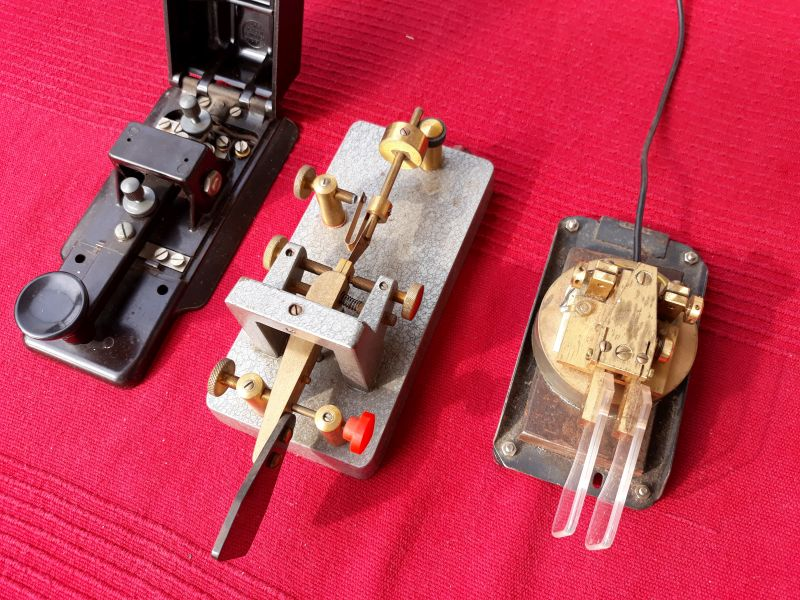
\includegraphics[width=0.85\textwidth]{foto/109}
    \caption{\scriptsize Morsetasten}
    \label{n_cwtast}
\end{figure}

   \end{column}
\end{columns}

\end{frame}

\begin{frame}
\begin{figure}
    
\includegraphics[width=0.85\textwidth]{foto/216}
    \caption{\scriptsize \enquote{CQ CQ} in Morsetelegrafie}
    \label{n_cqcq_horiz}
\end{figure}
\begin{itemize}
  \item Einigung darauf, was bestimmte Abfolgen unterschiedlicher Zeitabstände bedeuten
  \item Mitte des 19. Jahrhunderts Verständigung über den bis heute üblichen Morsecode
  \end{itemize}

\end{frame}

\begin{frame}
\frametitle{Telegrafie}
\begin{itemize}
  \item Übertragungsverfahren mit Hilfsmittel
  \item Rauch oder elektrische Schwingung wird so beeinflusst, um eine Nachricht zu übertragen
  \item Das Hilfsmittel ist der \emph{Träger}
  \item Im Funk aufgrund hoher Frequenzen auch \emph{Hochfrequenz-Träger} oder \emph{HF-Träger}
  \item Verfahren zum Ändern des Trägers ist die \emph{Modulation}
  \end{itemize}

\end{frame}

\begin{frame}
\only<1>{
\begin{QQuestion}{NE201}{Wie werden bei \glqq CW\grqq{} (Continuous Wave) Informationen übertragen?}{Durch Ein- und Ausschalten eines HF-Trägers}
{Durch Änderung der Trägerfrequenz in diskreten Stufen}
{Durch Modulation eines Subträgers}
{Durch diskrete Phasenmodulation}
\end{QQuestion}

}
\only<2>{
\begin{QQuestion}{NE201}{Wie werden bei \glqq CW\grqq{} (Continuous Wave) Informationen übertragen?}{\textbf{\textcolor{DARCgreen}{Durch Ein- und Ausschalten eines HF-Trägers}}}
{Durch Änderung der Trägerfrequenz in diskreten Stufen}
{Durch Modulation eines Subträgers}
{Durch diskrete Phasenmodulation}
\end{QQuestion}

}
\end{frame}

\begin{frame}
\only<1>{
\begin{QQuestion}{NE101}{Durch Modulation~...}{werden dem Signal NF-Komponenten entnommen.}
{wird einem oder mehreren Trägern Informationen entnommen.}
{werden Sprach- und CW-Signale kombiniert.}
{werden Informationen auf einen oder mehrere Träger übertragen.}
\end{QQuestion}

}
\only<2>{
\begin{QQuestion}{NE101}{Durch Modulation~...}{werden dem Signal NF-Komponenten entnommen.}
{wird einem oder mehreren Trägern Informationen entnommen.}
{werden Sprach- und CW-Signale kombiniert.}
{\textbf{\textcolor{DARCgreen}{werden Informationen auf einen oder mehrere Träger übertragen.}}}
\end{QQuestion}

}
\end{frame}

\begin{frame}
\frametitle{Andere Modulationsarten}
Die elektrische Schwingung kann auf andere Arten moduliert werden

\begin{itemize}
  \item Stärke (Amplitude)
  \item Periode (Frequenz)
  \end{itemize}
\end{frame}%ENDCONTENT


\section{Modulationsarten}
\label{section:modulationsarten}
\begin{frame}%STARTCONTENT

\begin{columns}
    \begin{column}{0.48\textwidth}
    
\begin{figure}
    \DARCimage{0.85\linewidth}{790include}
    \caption{\scriptsize Schwingung}
    \label{n_schwingung}
\end{figure}


    \end{column}
   \begin{column}{0.48\textwidth}
       Eigenschaften einer elektrischen Schwingung:

\begin{itemize}
  \item Amplitude
  \item Frequenz
  \end{itemize}

   \end{column}
\end{columns}

\end{frame}

\begin{frame}
\frametitle{Amplitudenmodulation (AM)}

\begin{figure}
    \DARCimage{0.85\linewidth}{358include}
    \caption{\scriptsize Bei der Amplitudenmodulation (AM) wird die Amplitude einer elektrischen Schwingung verändert.}
    \label{n_modulationsarten_am}
\end{figure}

\end{frame}

\begin{frame}
\frametitle{Frequenzmodulation (FM)}

\begin{figure}
    \DARCimage{0.85\linewidth}{357include}
    \caption{\scriptsize Bei der Frequenzmodulation (FM) wird die Schwingungsdauer und somit die Frequenz verändert.}
    \label{n_modulationsarten_am}
\end{figure}

\end{frame}%ENDCONTENT


\section{Sprachsignale}
\label{section:sprachsignale}
\begin{frame}%STARTCONTENT

\begin{figure}
    \DARCimage{0.85\linewidth}{742include}
    \caption{\scriptsize Menschliche Sprache im Amplitudenspektrum, links die tiefen und rechts die hohen Töne}
    \label{n_sprachspektrum}
\end{figure}

\end{frame}

\begin{frame}
\begin{columns}
    \begin{column}{0.48\textwidth}
    \begin{itemize}
  \item Sprechen wir in ein Mikrofon, dann wandelt es das Sprachsignal in elektrische Schwingungen um.
  \item Das Sprachsignal liegt nicht mehr als Schallwelle, sondern als elektrische Schwingung vor und kann im Funkgerät verarbeitet werden.
  \end{itemize}

    \end{column}
    \pause
    
   \begin{column}{0.48\textwidth}
       \begin{itemize}
  \item Die „Breite“ des Signals wird übrigens als \emph{Bandbreite} bezeichnet und in Hertz (Hz) angegeben.
  \item Angenommen es soll Sprache im Frequenzbereich von \qtyrange{300}{2700}{\hertz} übertragen werden.
  \item Die Bandbreite beträgt in diesem Falle \qty{2700}{\hertz} – \qty{300}{\hertz} = \qty{2400}{\hertz}
  \end{itemize}

   \end{column}
\end{columns}



\end{frame}

\begin{frame}
\only<1>{
\begin{QQuestion}{EA105}{Welche Einheit wird üblicherweise für die Bandbreite verwendet?}{Dezibel (dB)}
{Baud (Bd)}
{Bit pro Sekunde (Bit/s)}
{Hertz (Hz)}
\end{QQuestion}

}
\only<2>{
\begin{QQuestion}{EA105}{Welche Einheit wird üblicherweise für die Bandbreite verwendet?}{Dezibel (dB)}
{Baud (Bd)}
{Bit pro Sekunde (Bit/s)}
{\textbf{\textcolor{DARCgreen}{Hertz (Hz)}}}
\end{QQuestion}

}
\end{frame}%ENDCONTENT


\section{Amplitudenmodulation (AM)}
\label{section:am}
\begin{frame}%STARTCONTENT

\begin{columns}
    \begin{column}{0.48\textwidth}
    
\begin{figure}
    \DARCimage{0.85\linewidth}{716include}
    \caption{\scriptsize Signal eines AM-Rundfunksenders (Sprache / Musik)}
    \label{n_Wasserfall0}
\end{figure}


    \end{column}
   \begin{column}{0.48\textwidth}
       \begin{itemize}
  \item Modulationssignal wird durch Änderung der Amplitude auf den Träger aufmoduliert
  \item Frequenz des Trägers bleibt unverändert
  \item Änderung der Amplitude ändert die Form des Trägers $\rightarrow$ entspricht nicht mehr einer Sinusschwingung
  \item Zusätzliche Frequenzen heißen \emph{Seitenbänder}
  \end{itemize}

   \end{column}
\end{columns}

\end{frame}

\begin{frame}
\begin{columns}
    \begin{column}{0.48\textwidth}
    \begin{itemize}
  \item In den Seitenbändern steckt die übertragene Information, also z.\,B. die Sprache
  \item Die von AM belegte \emph{Bandbreite} ist doppelt so hoch wie die höchste Frequenz des Modulationssignals
  \end{itemize}

    \end{column}
   \begin{column}{0.48\textwidth}
       
\begin{figure}
    \DARCimage{0.85\linewidth}{476include}
    \caption{\scriptsize Symbolische Darstellung eines amplitudenmodulierten Signals mit Träger und Seitenbändern}
    \label{n_seitenband}
\end{figure}


   \end{column}
\end{columns}

\end{frame}

\begin{frame}
\only<1>{
\begin{QQuestion}{NE202}{Welche Aussage zur Amplitudenmodulation ist richtig? Durch das Informationssignal~...}{wird die Amplitude des Trägers beeinflusst. Die Frequenz des Trägers bleibt dabei konstant.}
{wird die Frequenz des Trägers beeinflusst. Die Amplitude des Trägers bleibt dabei konstant.}
{werden gleichzeitig Amplitude und Frequenz des Trägers beeinflusst.}
{werden nacheinander Amplitude und Frequenz des Trägers beeinflusst.}
\end{QQuestion}

}
\only<2>{
\begin{QQuestion}{NE202}{Welche Aussage zur Amplitudenmodulation ist richtig? Durch das Informationssignal~...}{\textbf{\textcolor{DARCgreen}{wird die Amplitude des Trägers beeinflusst. Die Frequenz des Trägers bleibt dabei konstant.}}}
{wird die Frequenz des Trägers beeinflusst. Die Amplitude des Trägers bleibt dabei konstant.}
{werden gleichzeitig Amplitude und Frequenz des Trägers beeinflusst.}
{werden nacheinander Amplitude und Frequenz des Trägers beeinflusst.}
\end{QQuestion}

}
\end{frame}

\begin{frame}
\only<1>{
\begin{PQuestion}{NE206}{Welche spektrale Darstellung ergibt sich für die Modulationsart AM bei diesem  Audiospektrum?}{\DARCimage{1.0\linewidth}{477include}}
{\DARCimage{1.0\linewidth}{476include}}
{\DARCimage{1.0\linewidth}{478include}}
{\DARCimage{1.0\linewidth}{479include}}
{\DARCimage{1.0\linewidth}{475include}}\end{PQuestion}

}
\only<2>{
\begin{PQuestion}{NE206}{Welche spektrale Darstellung ergibt sich für die Modulationsart AM bei diesem  Audiospektrum?}{\DARCimage{1.0\linewidth}{477include}}
{\textbf{\textcolor{DARCgreen}{\DARCimage{1.0\linewidth}{476include}}}}
{\DARCimage{1.0\linewidth}{478include}}
{\DARCimage{1.0\linewidth}{479include}}
{\DARCimage{1.0\linewidth}{475include}}\end{PQuestion}

}
\end{frame}%ENDCONTENT


\section{Einseitenbandmodulation (SSB)}
\label{section:ssb}
\begin{frame}%STARTCONTENT

\begin{columns}
    \begin{column}{0.48\textwidth}
    
\begin{figure}
    \DARCimage{0.85\linewidth}{482include}
    \caption{\scriptsize Amplitudenmodulation, Träger mit unterem (a) und oberen (b) Seitenband}
    \label{n_seitenband}
\end{figure}


    \end{column}
   \begin{column}{0.48\textwidth}
       \begin{itemize}
  \item Bei Amplitudenmodulation zusätzlich zum Träger zwei Seitenbänder $\rightarrow$ unteres bzw. oberes Seitenband
  \item \enquote{lower side band} (\emph{LSB}) und \enquote{upper side band} (\emph{USB})
  \item Der Träger selbst enthält gar keine Information
  \end{itemize}

   \end{column}
\end{columns}

\end{frame}

\begin{frame}
\begin{columns}
    \begin{column}{0.48\textwidth}
    \begin{itemize}
  \item Es reicht also, nur ein Seitenband auszusenden und auf den Träger und das andere Seitenband zu verzichten
  \item Gesamte Sendeleistung wird für die Übertragung der Information genutzt
  \item Belegte Bandbreite entspricht der Bandbreite des aufmodulierten Signals
  \end{itemize}

    \end{column}
   \begin{column}{0.48\textwidth}
       
\begin{figure}
    \DARCimage{0.85\linewidth}{743include}
    \caption{\scriptsize Seitenbänder bei AM, LSB und USB im Vergleich}
    \label{n_seitenband}
\end{figure}

\emph{Einseitenbandmodulation} bzw. \emph{single-sideband (SSB)}


   \end{column}
\end{columns}

\end{frame}

\begin{frame}USB steht für \emph{Upper Side Band}

(im Deutschen wird es gerne mit Unteres Seitenband verwechselt)

\end{frame}

\begin{frame}
\only<1>{
\begin{QQuestion}{NE203}{Was ist der Unterschied zwischen AM und SSB?}{AM hat keinen Träger und zwei Seitenbänder, SSB arbeitet mit Träger und nur einem Seitenband.}
{AM hat einen Träger und ein Seitenband, SSB arbeitet mit Trägerunterdrückung und hat zwei Seitenbänder.}
{AM hat keinen Träger und zwei Seitenbänder, SSB arbeitet mit Trägerunterdrückung und nur einem Seitenband.}
{AM hat einen Träger und zwei Seitenbänder, SSB arbeitet mit Trägerunterdrückung und nur einem Seitenband.}
\end{QQuestion}

}
\only<2>{
\begin{QQuestion}{NE203}{Was ist der Unterschied zwischen AM und SSB?}{AM hat keinen Träger und zwei Seitenbänder, SSB arbeitet mit Träger und nur einem Seitenband.}
{AM hat einen Träger und ein Seitenband, SSB arbeitet mit Trägerunterdrückung und hat zwei Seitenbänder.}
{AM hat keinen Träger und zwei Seitenbänder, SSB arbeitet mit Trägerunterdrückung und nur einem Seitenband.}
{\textbf{\textcolor{DARCgreen}{AM hat einen Träger und zwei Seitenbänder, SSB arbeitet mit Trägerunterdrückung und nur einem Seitenband.}}}
\end{QQuestion}

}
\end{frame}

\begin{frame}
\only<1>{
\begin{QQuestion}{NE204}{Was ist der Unterschied zwischen LSB und USB?}{LSB arbeitet mit Trägerunterdrückung und dem unteren Seitenband, USB arbeitet mit Trägerunterdrückung und dem oberen Seitenband.}
{LSB arbeitet mit Träger und zwei Seitenbändern, USB arbeitet mit Trägerunterdrückung und einem Seitenband.}
{LSB arbeitet mit Träger und einem Seitenband, USB arbeitet mit Trägerunterdrückung und beiden Seitenbändern.}
{LSB arbeitet mit Trägerunterdrückung und dem linken Seitenband, USB arbeitet mit Trägerunterdrückung und dem unteren Seitenband.}
\end{QQuestion}

}
\only<2>{
\begin{QQuestion}{NE204}{Was ist der Unterschied zwischen LSB und USB?}{\textbf{\textcolor{DARCgreen}{LSB arbeitet mit Trägerunterdrückung und dem unteren Seitenband, USB arbeitet mit Trägerunterdrückung und dem oberen Seitenband.}}}
{LSB arbeitet mit Träger und zwei Seitenbändern, USB arbeitet mit Trägerunterdrückung und einem Seitenband.}
{LSB arbeitet mit Träger und einem Seitenband, USB arbeitet mit Trägerunterdrückung und beiden Seitenbändern.}
{LSB arbeitet mit Trägerunterdrückung und dem linken Seitenband, USB arbeitet mit Trägerunterdrückung und dem unteren Seitenband.}
\end{QQuestion}

}
\end{frame}

\begin{frame}
\only<1>{
\begin{PQuestion}{NE208}{Welche spektrale Darstellung ergibt sich für Einseitenbandmodulation in LSB bei diesem Audiospektrum?}{\DARCimage{1.0\linewidth}{477include}}
{\DARCimage{1.0\linewidth}{480include}}
{\DARCimage{1.0\linewidth}{479include}}
{\DARCimage{1.0\linewidth}{481include}}
{\DARCimage{1.0\linewidth}{475include}}\end{PQuestion}

}
\only<2>{
\begin{PQuestion}{NE208}{Welche spektrale Darstellung ergibt sich für Einseitenbandmodulation in LSB bei diesem Audiospektrum?}{\DARCimage{1.0\linewidth}{477include}}
{\DARCimage{1.0\linewidth}{480include}}
{\DARCimage{1.0\linewidth}{479include}}
{\textbf{\textcolor{DARCgreen}{\DARCimage{1.0\linewidth}{481include}}}}
{\DARCimage{1.0\linewidth}{475include}}\end{PQuestion}

}
\end{frame}

\begin{frame}
\only<1>{
\begin{PQuestion}{NE207}{Welche spektrale Darstellung ergibt sich für Einseitenbandmodulation in USB bei diesem Audiospektrum?}{\DARCimage{1.0\linewidth}{481include}}
{\DARCimage{1.0\linewidth}{480include}}
{\DARCimage{1.0\linewidth}{479include}}
{\DARCimage{1.0\linewidth}{477include}}
{\DARCimage{1.0\linewidth}{475include}}\end{PQuestion}

}
\only<2>{
\begin{PQuestion}{NE207}{Welche spektrale Darstellung ergibt sich für Einseitenbandmodulation in USB bei diesem Audiospektrum?}{\DARCimage{1.0\linewidth}{481include}}
{\textbf{\textcolor{DARCgreen}{\DARCimage{1.0\linewidth}{480include}}}}
{\DARCimage{1.0\linewidth}{479include}}
{\DARCimage{1.0\linewidth}{477include}}
{\DARCimage{1.0\linewidth}{475include}}\end{PQuestion}

}
\end{frame}

\begin{frame}
\only<1>{
\begin{PQuestion}{NE205}{Welche Begriffe sind den Bereichen a und b des Modulationsverfahrens AM zuzuordnen?}{a = LSB; b = USB}
{a = USB; b = LSB}
{a = DSB; b = SSB}
{a = NF; b = HF}
{\DARCimage{1.0\linewidth}{482include}}\end{PQuestion}

}
\only<2>{
\begin{PQuestion}{NE205}{Welche Begriffe sind den Bereichen a und b des Modulationsverfahrens AM zuzuordnen?}{\textbf{\textcolor{DARCgreen}{a = LSB; b = USB}}}
{a = USB; b = LSB}
{a = DSB; b = SSB}
{a = NF; b = HF}
{\DARCimage{1.0\linewidth}{482include}}\end{PQuestion}

}
\end{frame}%ENDCONTENT


\section{Frequenzmodulation (FM)}
\label{section:fm}
\begin{frame}%STARTCONTENT

\begin{figure}
    \DARCimage{0.85\linewidth}{357include}
    \caption{\scriptsize Frequenzmodulation}
    \label{n_fm_frequenzmodulation}
\end{figure}

\begin{itemize}
  \item Modulationssignal wird durch Änderung der Frequenz auf den Träger aufmoduliert
  \item Amplitude des Trägers wird nicht verändert und bleibt idealerweise konstant
  \end{itemize}
\end{frame}

\begin{frame}
\only<1>{
\begin{QQuestion}{NE301}{Welche Aussage zur Frequenzmodulation ist richtig? Durch das Informationssignal~...}{wird die Frequenz des Trägers beeinflusst. Die Amplitude des Trägers bleibt dabei konstant.}
{wird die Amplitude des Trägers beeinflusst. Die Frequenz des Trägers bleibt dabei konstant. }
{werden gleichzeitig Frequenz und Amplitude des Trägers beeinflusst.}
{wird zuerst die Frequenz und dann die Amplitude des Trägers beeinflusst.}
\end{QQuestion}

}
\only<2>{
\begin{QQuestion}{NE301}{Welche Aussage zur Frequenzmodulation ist richtig? Durch das Informationssignal~...}{\textbf{\textcolor{DARCgreen}{wird die Frequenz des Trägers beeinflusst. Die Amplitude des Trägers bleibt dabei konstant.}}}
{wird die Amplitude des Trägers beeinflusst. Die Frequenz des Trägers bleibt dabei konstant. }
{werden gleichzeitig Frequenz und Amplitude des Trägers beeinflusst.}
{wird zuerst die Frequenz und dann die Amplitude des Trägers beeinflusst.}
\end{QQuestion}

}
\end{frame}

\begin{frame}
\only<1>{
\begin{QQuestion}{NE302}{Welche Antwort beschreibt die Modulationsart \glqq FM\grqq{}?}{Die Richtung eines Trägersignals wird anhand eines zu übertragenden Signals verändert.}
{Die Amplitude eines Trägersignals wird anhand eines zu übertragenden Signals verändert.}
{Die Polarisation eines Trägersignals wird anhand eines zu übertragenden Signals verändert.}
{Die Frequenz eines Trägersignals wird anhand eines zu übertragenden Signals verändert.}
\end{QQuestion}

}
\only<2>{
\begin{QQuestion}{NE302}{Welche Antwort beschreibt die Modulationsart \glqq FM\grqq{}?}{Die Richtung eines Trägersignals wird anhand eines zu übertragenden Signals verändert.}
{Die Amplitude eines Trägersignals wird anhand eines zu übertragenden Signals verändert.}
{Die Polarisation eines Trägersignals wird anhand eines zu übertragenden Signals verändert.}
{\textbf{\textcolor{DARCgreen}{Die Frequenz eines Trägersignals wird anhand eines zu übertragenden Signals verändert.}}}
\end{QQuestion}

}
\end{frame}

\begin{frame}
\only<1>{
\begin{QQuestion}{NE303}{Welche Auswirkung hat Frequenzmodulation (FM) auf die Amplitude des Sendesignals?}{Je schneller die Schwingung des Modulationssignals ist, umso größer wird die Amplitude des Sendesignals.}
{Idealerweise entspricht die Amplitude des Sendesignals der Amplitude des Modulationssignals.}
{Idealerweise hat das Modulationssignal keine Auswirkung auf die Amplitude des Sendesignals.}
{Je größer die Amplitude des Modulationssignals ist, umso größer wird die Amplitude des Sendesignals.}
\end{QQuestion}

}
\only<2>{
\begin{QQuestion}{NE303}{Welche Auswirkung hat Frequenzmodulation (FM) auf die Amplitude des Sendesignals?}{Je schneller die Schwingung des Modulationssignals ist, umso größer wird die Amplitude des Sendesignals.}
{Idealerweise entspricht die Amplitude des Sendesignals der Amplitude des Modulationssignals.}
{\textbf{\textcolor{DARCgreen}{Idealerweise hat das Modulationssignal keine Auswirkung auf die Amplitude des Sendesignals.}}}
{Je größer die Amplitude des Modulationssignals ist, umso größer wird die Amplitude des Sendesignals.}
\end{QQuestion}

}
\end{frame}

\begin{frame}
\frametitle{Frequenzhub}
\begin{itemize}
  \item Je lauter in das Mikrofon gesprochen wird, umso größer die Änderung der Trägerfrequenz
  \item Dadurch steigt auch die belegte Bandbreite der Aussendung
  \item Maximalwert der Änderung der Trägerfrequenz wird als \emph{Frequenzhub} oder kurz \emph{Hub} bezeichnet
  \item In der Praxis kommt Schmalband-FM (englisch Narrow- FM, kurz NFM) mit \qty{12}{\kilo\hertz} Bandbreite zum Einsatz
  \end{itemize}

\end{frame}

\begin{frame}
\only<1>{
\begin{QQuestion}{BC216}{Warum sollten Sie bei FM-Telefonie auf \qty{145,525}{\MHz} darauf achten, ihr Funkgerät auf Schmalband-FM (Narrow FM) einzustellen? Der IARU-Bandplan empfiehlt~...}{ein Kanalraster von \qty{5}{\kHz} einzuhalten.}
{in diesem Frequenzbereich nicht mehr als \qty{25}{\kHz} Bandbreite zu belegen.}
{einen Kanalabstand von \qty{50}{\kHz} einzuhalten.}
{in diesem Frequenzbereich nicht mehr als \qty{12}{\kHz} Bandbreite zu belegen.}
\end{QQuestion}

}
\only<2>{
\begin{QQuestion}{BC216}{Warum sollten Sie bei FM-Telefonie auf \qty{145,525}{\MHz} darauf achten, ihr Funkgerät auf Schmalband-FM (Narrow FM) einzustellen? Der IARU-Bandplan empfiehlt~...}{ein Kanalraster von \qty{5}{\kHz} einzuhalten.}
{in diesem Frequenzbereich nicht mehr als \qty{25}{\kHz} Bandbreite zu belegen.}
{einen Kanalabstand von \qty{50}{\kHz} einzuhalten.}
{\textbf{\textcolor{DARCgreen}{in diesem Frequenzbereich nicht mehr als \qty{12}{\kHz} Bandbreite zu belegen.}}}
\end{QQuestion}

}
\end{frame}

\begin{frame}
\only<1>{
\begin{QQuestion}{NE306}{Was kann man tun, wenn der Hub bei einem Handfunkgerät oder Mobil-Transceiver zu groß ist?}{Weniger Leistung verwenden}
{Lauter ins Mikrofon sprechen}
{Leiser ins Mikrofon sprechen}
{Mehr Leistung verwenden}
\end{QQuestion}

}
\only<2>{
\begin{QQuestion}{NE306}{Was kann man tun, wenn der Hub bei einem Handfunkgerät oder Mobil-Transceiver zu groß ist?}{Weniger Leistung verwenden}
{Lauter ins Mikrofon sprechen}
{\textbf{\textcolor{DARCgreen}{Leiser ins Mikrofon sprechen}}}
{Mehr Leistung verwenden}
\end{QQuestion}

}

\end{frame}

\begin{frame}
\only<1>{
\begin{QQuestion}{NE304}{Sie senden mit \qty{2}{\W} in FM auf dem \qty{70}{\cm}-Band. Wie groß ist die angezeigte Sendeleistung, wenn Sie zuerst laut, danach leise und dann nicht mehr in das Mikrofon sprechen?}{zuerst \qty{1}{\W}, dann \qty{0,5}{\W} und zum Schluss \qty{0}{\W}}
{zuerst \qty{2}{\W}, dann \qty{1}{\W} und zum Schluss \qty{0}{\W}}
{immer \qty{2}{\W}}
{immer \qty{1}{\W}}
\end{QQuestion}

}
\only<2>{
\begin{QQuestion}{NE304}{Sie senden mit \qty{2}{\W} in FM auf dem \qty{70}{\cm}-Band. Wie groß ist die angezeigte Sendeleistung, wenn Sie zuerst laut, danach leise und dann nicht mehr in das Mikrofon sprechen?}{zuerst \qty{1}{\W}, dann \qty{0,5}{\W} und zum Schluss \qty{0}{\W}}
{zuerst \qty{2}{\W}, dann \qty{1}{\W} und zum Schluss \qty{0}{\W}}
{\textbf{\textcolor{DARCgreen}{immer \qty{2}{\W}}}}
{immer \qty{1}{\W}}
\end{QQuestion}

}

\end{frame}%ENDCONTENT


\section{Bandbreite}
\label{section:bandbreite}
\begin{frame}%STARTCONTENT

\begin{columns}
    \begin{column}{0.48\textwidth}
    \begin{itemize}
  \item Für die verschiedenen Amateurfunkbänder sind jeweils maximal zulässige Bandbreiten festgelegt
  \item Besonders aufpassen muss man bei Sendungen in der Nähe der Grenzen der Amateurfunkbänder
  \end{itemize}

    \end{column}
    \pause
    
   \begin{column}{0.48\textwidth}
       \begin{itemize}
  \item Nehmen wir an, ein FM-Signal ist \qty{15}{\kilo\hertz} breit und wir senden auf auf \qty{430}{\mega\hertz}
  \item Das Sendesignal befindet sich jeweils \qty{7,5}{\kilo\hertz} unterhalb und oberhalb
  \item Es würde sich also von \qtyrange{429,9925}{430,0075}{\mega\hertz} erstrecken
  \end{itemize}

   \end{column}
\end{columns}

\end{frame}

\begin{frame}
\only<1>{
\begin{QQuestion}{NE305}{Die gesamte Bandbreite einer FM-Übertragung beträgt \qty{15}{\kHz}. Wie weit muss die am Transceiver eingestellte Sendefrequenz von einer Bandgrenze mindestens entfernt sein, damit die Aussendung innerhalb des Bandes bleibt?}{\qty{0}{\kHz}}
{\qty{7,5}{\kHz}}
{\qty{15}{\kHz}}
{\qty{2,7}{\kHz}}
\end{QQuestion}

}
\only<2>{
\begin{QQuestion}{NE305}{Die gesamte Bandbreite einer FM-Übertragung beträgt \qty{15}{\kHz}. Wie weit muss die am Transceiver eingestellte Sendefrequenz von einer Bandgrenze mindestens entfernt sein, damit die Aussendung innerhalb des Bandes bleibt?}{\qty{0}{\kHz}}
{\textbf{\textcolor{DARCgreen}{\qty{7,5}{\kHz}}}}
{\qty{15}{\kHz}}
{\qty{2,7}{\kHz}}
\end{QQuestion}

}
\end{frame}

\begin{frame}
\begin{columns}
    \begin{column}{0.48\textwidth}
    Bei SSB  ist das Signal nur auf einer Seite der Trägerfrequenz zu finden:

\begin{itemize}
  \item Bei LSB vollständig unterhalb der Trägerfrequenz
  \item Bei USB vollständig oberhalb der Trägerfrequenz
  \end{itemize}

    \end{column}
    \pause
    
   \begin{column}{0.48\textwidth}
       Beispiel:

\begin{itemize}
  \item Am Funkgerät Sendefrequenz auf obere Bandgrenze einstellen
  \item Mit LSB darf gesendet werden
  \item Mit USB ist das Signal außerhalb des Bandes
  \end{itemize}

   \end{column}
\end{columns}



\end{frame}

\begin{frame}
\only<1>{
\begin{QQuestion}{VD738}{In welchen Amateurfunkfrequenzbereichen beträgt die maximal zulässige belegte Bandbreite einer Aussendung \qty{800}{\Hz}?}{\qtyrange{18068}{18168}{\kHz} und \qtyrange{24890}{24990}{\kHz}}
{\qtyrange{1810}{2000}{\kHz}, \qtyrange{3500}{3800}{\kHz} und \qtyrange{7000}{7200}{\kHz}}
{\qtyrange{7000}{7100}{\kHz} und \qtyrange{14000}{14350}{\kHz}}
{\qtyrange{135,7}{137,8}{\kHz}, \qtyrange{472}{479}{\kHz} und \qtyrange{10100}{10150}{\kHz}}
\end{QQuestion}

}
\only<2>{
\begin{QQuestion}{VD738}{In welchen Amateurfunkfrequenzbereichen beträgt die maximal zulässige belegte Bandbreite einer Aussendung \qty{800}{\Hz}?}{\qtyrange{18068}{18168}{\kHz} und \qtyrange{24890}{24990}{\kHz}}
{\qtyrange{1810}{2000}{\kHz}, \qtyrange{3500}{3800}{\kHz} und \qtyrange{7000}{7200}{\kHz}}
{\qtyrange{7000}{7100}{\kHz} und \qtyrange{14000}{14350}{\kHz}}
{\textbf{\textcolor{DARCgreen}{\qtyrange{135,7}{137,8}{\kHz}, \qtyrange{472}{479}{\kHz} und \qtyrange{10100}{10150}{\kHz}}}}
\end{QQuestion}

}
\end{frame}

\begin{frame}
\only<1>{
\begin{QQuestion}{VD739}{In welchem der folgenden Amateurfunkfrequenzbereiche beträgt die maximal zulässige belegte Bandbreite einer Aussendung \qty{2,7}{\kHz}?}{\qtyrange{135,7}{137,8}{\kHz}}
{\qtyrange{10100}{10150}{\kHz}}
{\qtyrange{3500}{3800}{\kHz}}
{\qtyrange{28000}{29700}{\kHz}}
\end{QQuestion}

}
\only<2>{
\begin{QQuestion}{VD739}{In welchem der folgenden Amateurfunkfrequenzbereiche beträgt die maximal zulässige belegte Bandbreite einer Aussendung \qty{2,7}{\kHz}?}{\qtyrange{135,7}{137,8}{\kHz}}
{\qtyrange{10100}{10150}{\kHz}}
{\textbf{\textcolor{DARCgreen}{\qtyrange{3500}{3800}{\kHz}}}}
{\qtyrange{28000}{29700}{\kHz}}
\end{QQuestion}

}
\end{frame}

\begin{frame}
\only<1>{
\begin{QQuestion}{VD740}{In welchem der folgenden Amateurfunkfrequenzbereiche beträgt die maximal zulässige belegte Bandbreite einer Aussendung \qty{7}{\kHz}?}{\qtyrange{21000}{21450}{\kHz}}
{\qtyrange{14000}{14350}{\kHz}}
{\qtyrange{28000}{29000}{\kHz}}
{\qtyrange{10100}{10150}{\kHz}}
\end{QQuestion}

}
\only<2>{
\begin{QQuestion}{VD740}{In welchem der folgenden Amateurfunkfrequenzbereiche beträgt die maximal zulässige belegte Bandbreite einer Aussendung \qty{7}{\kHz}?}{\qtyrange{21000}{21450}{\kHz}}
{\qtyrange{14000}{14350}{\kHz}}
{\textbf{\textcolor{DARCgreen}{\qtyrange{28000}{29000}{\kHz}}}}
{\qtyrange{10100}{10150}{\kHz}}
\end{QQuestion}

}
\end{frame}

\begin{frame}
\only<1>{
\begin{QQuestion}{VD741}{In welchem der folgenden Amateurfunkfrequenzbereiche beträgt die maximal zulässige belegte Bandbreite einer Aussendung \qty{40}{\kHz}?}{\qtyrange{144}{146}{\MHz}}
{\qtyrange{430}{440}{\MHz}}
{\qtyrange{1240}{1300}{\MHz}}
{\qtyrange{7000}{7200}{\kHz}}
\end{QQuestion}

}
\only<2>{
\begin{QQuestion}{VD741}{In welchem der folgenden Amateurfunkfrequenzbereiche beträgt die maximal zulässige belegte Bandbreite einer Aussendung \qty{40}{\kHz}?}{\textbf{\textcolor{DARCgreen}{\qtyrange{144}{146}{\MHz}}}}
{\qtyrange{430}{440}{\MHz}}
{\qtyrange{1240}{1300}{\MHz}}
{\qtyrange{7000}{7200}{\kHz}}
\end{QQuestion}

}
\end{frame}

\begin{frame}
\only<1>{
\begin{QQuestion}{VD742}{In welchem der folgenden Amateurfunkfrequenzbereiche beträgt die maximal zulässige belegte Bandbreite einer Aussendung \qty{2}{\MHz} bzw. für amplitudenmodulierte Fernsehaussendungen \qty{7}{\MHz}?}{\qtyrange{2320}{2450}{\MHz}}
{\qtyrange{430}{440}{\MHz}}
{\qtyrange{3400}{3475}{\MHz}}
{\qtyrange{10,0}{10,5}{\GHz}}
\end{QQuestion}

}
\only<2>{
\begin{QQuestion}{VD742}{In welchem der folgenden Amateurfunkfrequenzbereiche beträgt die maximal zulässige belegte Bandbreite einer Aussendung \qty{2}{\MHz} bzw. für amplitudenmodulierte Fernsehaussendungen \qty{7}{\MHz}?}{\qtyrange{2320}{2450}{\MHz}}
{\textbf{\textcolor{DARCgreen}{\qtyrange{430}{440}{\MHz}}}}
{\qtyrange{3400}{3475}{\MHz}}
{\qtyrange{10,0}{10,5}{\GHz}}
\end{QQuestion}

}
\end{frame}%ENDCONTENT


\section{Modulationseinstellungen am Funkgerät}
\label{section:trxmodulation}
\begin{frame}%STARTCONTENT
\begin{itemize}
  \item An vielen Funkgeräten gibt es einen Schalter, um die Modulationsart auszuwählen
  \item Meistens ist dieser mit „Mode“ beschriftet und erlaubt beispielsweise zwischen CW, AM, FM und SSB zu wählen
  \end{itemize}
\end{frame}

\begin{frame}
\only<1>{
\begin{QQuestion}{NE102}{In welcher der folgenden Antwortmöglichkeiten sind ausschließlich Modulationsarten enthalten? }{THOR, Olivia, FreeDV}
{RTTY, PSK31, SSTV}
{M17, FT8, JS8}
{SSB, FM, AM}
\end{QQuestion}

}
\only<2>{
\begin{QQuestion}{NE102}{In welcher der folgenden Antwortmöglichkeiten sind ausschließlich Modulationsarten enthalten? }{THOR, Olivia, FreeDV}
{RTTY, PSK31, SSTV}
{M17, FT8, JS8}
{\textbf{\textcolor{DARCgreen}{SSB, FM, AM}}}
\end{QQuestion}

}

\end{frame}

\begin{frame}\begin{itemize}
  \item Bei SSB ist zu beachten, das richtige Seitenband (LSB oder USB) auszuwählen
  \item Im Amateurfunk wird mit wenigen Ausnahmen unterhalb von \qty{10}{\mega\hertz} das untere Seitenband und ab \qty{10}{\mega\hertz} das obere Seitenband benutzt
  \end{itemize}

\end{frame}

\begin{frame}
\only<1>{
\begin{PQuestion}{NE209}{Die Darstellung zeigt das Display eines Transceivers. Was bedeutet die Anzeige \glqq USB\grqq{}?}{Der \glqq Untere Schmalband Betrieb\grqq{} ist aktiviert. }
{Der Transceiver empfängt in der Modulationsart SSB im unteren Seitenband.}
{Der Transceiver empfängt in der Modulationsart SSB im oberen Seitenband.}
{Die Unterspannung der Batterie ist erreicht.}
{\DARCimage{1.0\linewidth}{588include}}\end{PQuestion}

}
\only<2>{
\begin{PQuestion}{NE209}{Die Darstellung zeigt das Display eines Transceivers. Was bedeutet die Anzeige \glqq USB\grqq{}?}{Der \glqq Untere Schmalband Betrieb\grqq{} ist aktiviert. }
{Der Transceiver empfängt in der Modulationsart SSB im unteren Seitenband.}
{\textbf{\textcolor{DARCgreen}{Der Transceiver empfängt in der Modulationsart SSB im oberen Seitenband.}}}
{Die Unterspannung der Batterie ist erreicht.}
{\DARCimage{1.0\linewidth}{588include}}\end{PQuestion}

}
\end{frame}

\begin{frame}
\only<1>{
\begin{QQuestion}{BC202}{Welches Seitenband wird bei SSB-Telefonie nach IARU-Empfehlung im \qty{80}{m}-Band in der Regel benutzt?}{In der unteren Bandhälfte das untere Seitenband, in der oberen Bandhälfte das obere Seitenband.}
{Im Europaverkehr wird das untere, ansonsten das obere Seitenband benutzt.}
{Um den Nachteil der relativ niedrigen Sendefrequenz des \qty{80}{m}-Bandes auszugleichen, wird das obere Seitenband benutzt.}
{Im \qty{80}{m}-Band wird das untere Seitenband benutzt.}
\end{QQuestion}

}
\only<2>{
\begin{QQuestion}{BC202}{Welches Seitenband wird bei SSB-Telefonie nach IARU-Empfehlung im \qty{80}{m}-Band in der Regel benutzt?}{In der unteren Bandhälfte das untere Seitenband, in der oberen Bandhälfte das obere Seitenband.}
{Im Europaverkehr wird das untere, ansonsten das obere Seitenband benutzt.}
{Um den Nachteil der relativ niedrigen Sendefrequenz des \qty{80}{m}-Bandes auszugleichen, wird das obere Seitenband benutzt.}
{\textbf{\textcolor{DARCgreen}{Im \qty{80}{m}-Band wird das untere Seitenband benutzt.}}}
\end{QQuestion}

}
\end{frame}

\begin{frame}
\only<1>{
\begin{QQuestion}{BC203}{Welches Seitenband wird bei SSB-Telefonie nach Empfehlung der IARU im \qty{20}{m}-Band in der Regel benutzt?}{Um den Nachteil der relativ niedrigen Sendefrequenz des \qty{20}{m}-Bandes auszugleichen, wird das untere Seitenband benutzt.}
{Im Europaverkehr wird das untere, ansonsten das obere Seitenband benutzt.}
{Im \qty{20}{m}-Band wird das obere Seitenband benutzt.}
{In der unteren Bandhälfte das untere Seitenband, in der oberen Bandhälfte das obere Seitenband.}
\end{QQuestion}

}
\only<2>{
\begin{QQuestion}{BC203}{Welches Seitenband wird bei SSB-Telefonie nach Empfehlung der IARU im \qty{20}{m}-Band in der Regel benutzt?}{Um den Nachteil der relativ niedrigen Sendefrequenz des \qty{20}{m}-Bandes auszugleichen, wird das untere Seitenband benutzt.}
{Im Europaverkehr wird das untere, ansonsten das obere Seitenband benutzt.}
{\textbf{\textcolor{DARCgreen}{Im \qty{20}{m}-Band wird das obere Seitenband benutzt.}}}
{In der unteren Bandhälfte das untere Seitenband, in der oberen Bandhälfte das obere Seitenband.}
\end{QQuestion}

}
\end{frame}

\begin{frame}
\only<1>{
\begin{QQuestion}{NE211}{Im \qty{80}{\m}-Band wird bei Sprechfunk das Modulationsverfahren SSB \glqq Unteres Seitenband\grqq{} verwendet. Auf welchen \glqq MODE\grqq{} stellen Sie den Amateurfunk-Empfänger ein?}{LSB}
{USB}
{AM}
{SSB}
\end{QQuestion}

}
\only<2>{
\begin{QQuestion}{NE211}{Im \qty{80}{\m}-Band wird bei Sprechfunk das Modulationsverfahren SSB \glqq Unteres Seitenband\grqq{} verwendet. Auf welchen \glqq MODE\grqq{} stellen Sie den Amateurfunk-Empfänger ein?}{\textbf{\textcolor{DARCgreen}{LSB}}}
{USB}
{AM}
{SSB}
\end{QQuestion}

}
\end{frame}

\begin{frame}
\only<1>{
\begin{QQuestion}{NE210}{Im \qty{2}{\m}-Band wird das \glqq obere Seitenband\grqq{} verwendet. Auf welchen \glqq MODE\grqq{} stellen Sie den Amateurfunk-Transceiver ein?}{LSB}
{USB}
{FM}
{CW}
\end{QQuestion}

}
\only<2>{
\begin{QQuestion}{NE210}{Im \qty{2}{\m}-Band wird das \glqq obere Seitenband\grqq{} verwendet. Auf welchen \glqq MODE\grqq{} stellen Sie den Amateurfunk-Transceiver ein?}{LSB}
{\textbf{\textcolor{DARCgreen}{USB}}}
{FM}
{CW}
\end{QQuestion}

}
\end{frame}

\begin{frame}
\frametitle{Falsches Seitenband}
\begin{itemize}
  \item Wenn bei SSB das falsche Seitenband gewählt wird, dann ist die Sprache völlig unverständlich
  \item Ebenfalls ist es bei SSB wichtig, die Empfangsfrequenz sehr feinfühlig mit dem VFO-Drehknopf einzustellen
  \item Schon kleine Abweichungen von der richtigen Frequenz führen dazu, dass die Sprache unverständlich wird
  \end{itemize}

\end{frame}

\begin{frame}
\only<1>{
\begin{QQuestion}{NE212}{Sie können die Sprache beim SSB-Empfang nicht verstehen. Welche Vorgehensweise führt zum Ziel?}{Sie drehen am VFO-Knopf und drücken die TUNE-Taste.}
{Sie kontrollieren die Seitenbandeinstellung und drehen am VFO-Knopf.}
{Sie drehen am RIT-Knopf und drücken die PTT.}
{Sie beobachten das Wasserfalldiagramm und wechseln in die Modulationsart AM.}
\end{QQuestion}

}
\only<2>{
\begin{QQuestion}{NE212}{Sie können die Sprache beim SSB-Empfang nicht verstehen. Welche Vorgehensweise führt zum Ziel?}{Sie drehen am VFO-Knopf und drücken die TUNE-Taste.}
{\textbf{\textcolor{DARCgreen}{Sie kontrollieren die Seitenbandeinstellung und drehen am VFO-Knopf.}}}
{Sie drehen am RIT-Knopf und drücken die PTT.}
{Sie beobachten das Wasserfalldiagramm und wechseln in die Modulationsart AM.}
\end{QQuestion}

}
\end{frame}%ENDCONTENT


\title{DARC Amateurfunklehrgang Klasse N}
\author{Digitale Übertragungsverfahren}
\institute{Deutscher Amateur Radio Club e.\,V.}
\begin{frame}
\maketitle
\end{frame}

\section{Analog vs. Digital}
\label{section:analog_vs_digital}
\begin{frame}%STARTCONTENT

\begin{columns}
    \begin{column}{0.48\textwidth}
    Bei der Informationsübertragung unterscheidet man grundsätzlich zwischen analogen und digitalen Verfahren.

\begin{itemize}
  \item \emph{Digital}: in Stufen, nur bestimmte Werte, keine Werte dazwischen
  \item \emph{Analog}: kontinuierlich, beliebige Zwischenwerte
  \end{itemize}

    \end{column}
   \begin{column}{0.48\textwidth}
       
\begin{figure}
    \DARCimage{0.85\linewidth}{411include}
    \caption{\scriptsize Digitales Signal (abgestuft)}
    \label{n_digital_einleitung_digitales_signal}
\end{figure}


\begin{figure}
    \DARCimage{0.85\linewidth}{408include}
    \caption{\scriptsize Analoges Signal (kontinuierlich)}
    \label{n_digital_einleitung_analoges_signal}
\end{figure}


   \end{column}
\end{columns}

\end{frame}%ENDCONTENT


\section{Morsetelegrafie}
\label{section:morsetelegrafie}
\begin{frame}%STARTCONTENT
\begin{itemize}
  \item Ein- und Ausschalten eines Trägers
  \item Einführung eines \emph{Morsealphabets} 1838 durch Samuel Morse, optimiert durch Friedrich Clemens Gerke
  \item Morseprüfung lange Zeit Vorschrift für Funkamateure auf Kurzwelle
  \item Seit Mitte der 1990er legen Länder fest, ob \emph{Morseprüfung} notwendig ist
  \item Erst seit 2003 ist die Morseprüfung in Deutschland freiwillig
  \end{itemize}

\end{frame}

\begin{frame}\begin{table}
\begin{DARCtabular}{clclcl}
    ~  &~   &~   &~   &~   &~    \\
     A  & \MorseDit\MorseDah  & K  & \MorseDah\MorseDit\MorseDah  & U  & \MorseDit\MorseDit\MorseDah   \\
     B  & \MorseDah\MorseDit\MorseDit\MorseDit  & L  & \MorseDit\MorseDah\MorseDit\MorseDit  & V  & \MorseDit\MorseDit\MorseDit\MorseDah   \\
     C  & \MorseDah\MorseDit\MorseDah\MorseDit  & M  & \MorseDah\MorseDah  & W  & \MorseDit\MorseDah\MorseDah   \\
     D  & \MorseDah\MorseDit\MorseDit  & N  & \MorseDah\MorseDit  & X  & \MorseDah\MorseDit\MorseDit\MorseDah   \\
     E  & \MorseDit  & O  & \MorseDah\MorseDah\MorseDah  & Y  & \MorseDah\MorseDit\MorseDah\MorseDah   \\
     F  & \MorseDit\MorseDit\MorseDah\MorseDit  & P  & \MorseDit\MorseDah\MorseDah\MorseDit  & Z  & \MorseDah\MorseDah\MorseDit\MorseDit   \\
     G  & \MorseDah\MorseDah\MorseDit  & Q  & \MorseDah\MorseDah\MorseDit\MorseDah  & Ä  & \MorseDit\MorseDah\MorseDit\MorseDah   \\
     H  & \MorseDit\MorseDit\MorseDit\MorseDit  & R  & \MorseDit\MorseDah\MorseDit  & Ö  & \MorseDah\MorseDah\MorseDah\MorseDit   \\
     I  & \MorseDit\MorseDit  & S  & \MorseDit\MorseDit\MorseDit  & Ü  & \MorseDit\MorseDit\MorseDah\MorseDah   \\
     J  & \MorseDit\MorseDah\MorseDah\MorseDah  & T  & \MorseDah  & ẞ  & \MorseDit\MorseDit\MorseDit\MorseDah\MorseDah\MorseDit\MorseDit   \\
\end{DARCtabular}
\caption{Morsecode (Buchstaben)}
\label{n_morsetelegrafie_morsecode_buchstaben}
\end{table}
\end{frame}

\begin{frame}\begin{table}
\begin{DARCtabular}{clclcl}
    ~   &~   &~   &~   &~   &~    \\
     0  & \MorseDah\MorseDah\MorseDah\MorseDah\MorseDah  & 5  & \MorseDit\MorseDit\MorseDit\MorseDit\MorseDit  & /  & \MorseDah\MorseDit\MorseDit\MorseDah\MorseDit   \\
     1  & \MorseDit\MorseDah\MorseDah\MorseDah\MorseDah  & 6  & \MorseDah\MorseDit\MorseDit\MorseDit\MorseDit  & .  & \MorseDit\MorseDah\MorseDit\MorseDah\MorseDit\MorseDah   \\
     2  & \MorseDit\MorseDit\MorseDah\MorseDah\MorseDah  & 7  & \MorseDah\MorseDah\MorseDit\MorseDit\MorseDit  & ,  & \MorseDah\MorseDah\MorseDit\MorseDit\MorseDah\MorseDah   \\
     3  & \MorseDit\MorseDit\MorseDit\MorseDah\MorseDah  & 8  & \MorseDah\MorseDah\MorseDah\MorseDit\MorseDit  & ?  & \MorseDit\MorseDit\MorseDah\MorseDah\MorseDit\MorseDit   \\
     4  & \MorseDit\MorseDit\MorseDit\MorseDit\MorseDah  & 9  & \MorseDah\MorseDah\MorseDah\MorseDah\MorseDit  & =  & \MorseDah\MorseDit\MorseDit\MorseDit\MorseDah   \\
\end{DARCtabular}
\caption{Morsecode (Ziffern und Satzzeichen)}
\label{n_morsetelegrafie_morsecode_ziffern_satzzeichen}
\end{table}
\begin{table}
\begin{DARCtabular}{ll}
    ~   &~    \\
     Unterbrechung (BK)  & \MorseDah\MorseDit\MorseDit\MorseDit\MorseDah\MorseDit\MorseDah   \\
     Ende des Durchgangs (AR)   & \MorseDit\MorseDah\MorseDit\MorseDah\MorseDit   \\
     Ende der Sendung (SK)  & \MorseDit\MorseDit\MorseDit\MorseDah\MorseDit\MorseDah   \\
     Korrektur  & \MorseDit\MorseDit\MorseDit\MorseDit\MorseDit\MorseDit\MorseDit\MorseDit   \\
\end{DARCtabular}
\caption{Morsecode (besondere Zeichen, Auswahl)}
\label{n_morsetelegrafie_morsecode_spezial}
\end{table}
\end{frame}

\begin{frame}
\only<1>{
\begin{QQuestion}{VA304}{Was ist in den Radio Regulations (RR) bezüglich der Morsequalifikation für Funkamateure festgelegt?}{Wer Frequenzen unter \qty{30}{\MHz} nutzen will, muss eine Morseprüfung ablegen.}
{Bei einer Sendeleistung von mehr als \qty{100}{\W} benötigt der Funkamateur den Nachweis einer erfolgreich abgelegten Morseprüfung.}
{Die nationale Verwaltung eines jeden Landes legt eigenständig fest, ob eine Morseprüfung erforderlich ist.}
{In den Radio Regulations (RR) werden bezüglich der Morsequalifikation keine Regelungen getroffen.}
\end{QQuestion}

}
\only<2>{
\begin{QQuestion}{VA304}{Was ist in den Radio Regulations (RR) bezüglich der Morsequalifikation für Funkamateure festgelegt?}{Wer Frequenzen unter \qty{30}{\MHz} nutzen will, muss eine Morseprüfung ablegen.}
{Bei einer Sendeleistung von mehr als \qty{100}{\W} benötigt der Funkamateur den Nachweis einer erfolgreich abgelegten Morseprüfung.}
{\textbf{\textcolor{DARCgreen}{Die nationale Verwaltung eines jeden Landes legt eigenständig fest, ob eine Morseprüfung erforderlich ist.}}}
{In den Radio Regulations (RR) werden bezüglich der Morsequalifikation keine Regelungen getroffen.}
\end{QQuestion}

}
\end{frame}%ENDCONTENT


\section{Computersteuerung}
\label{section:computersteuerung}
\begin{frame}%STARTCONTENT

\frametitle{Steuersignale}
\begin{columns}
    \begin{column}{0.48\textwidth}
    \begin{itemize}
  \item Übertragung von Audio- sowie Steuersignalen (CAT) zwischen Computer und Transceiver
  \item Z.B. Transceiver auf Sendung schalten und Signal vom Computer übertragen
  \end{itemize}

    \end{column}
   \begin{column}{0.48\textwidth}
       
\begin{figure}
    \DARCimage{0.85\linewidth}{630include}
    \caption{\scriptsize Beispiele für Verbindungen zwischen Computer und Funkgerät}
    \label{n_computersteuerung_verbindungen}
\end{figure}


   \end{column}
\end{columns}

\end{frame}

\begin{frame}
\frametitle{Datenanschluss}
\begin{itemize}
  \item Hinter dem Mikrofonanschluss im Funkgerät können Verstärker- und Filterstufen für Sprachübertragung liegen $\rightarrow$ ungeeignet für Datenübertragung
  \item Eigener Datenanschluss am Transceiver
  \item Lässt Signale vom Computer unverfälscht passieren
  \end{itemize}

\end{frame}

\begin{frame}
\only<1>{
\begin{QQuestion}{NF114}{Wie kann eine Verbindung zwischen Funkgerät und Computer für digitale Übertragungsverfahren (z.~B. FT8 oder WSPR) hergestellt werden?}{Der ALC-Anschluss des Funkgeräts wird mittels eines Hardware-Modems mit Audio- oder Datenanschlüssen des Computers verbunden.}
{Eine Audioverbindung (NF-Signal oder digital z.~B. per USB-Kabel) wird zwischen Computer und Funkgerät hergestellt oder es wird ein Hardware-Modem verwendet.}
{Es wird ein Software-Modem installiert und der ALC-Anschluss des Funkgeräts direkt mit dem Computer verbunden (ggf. auch mittels Adapter).}
{Der HF-Anschluss (z.~B. Antennenausgang) des Funkgeräts wird mittels eines Y-Kabels mit einer geeigneten Datenschnittstelle des Computers verbunden.}
\end{QQuestion}

}
\only<2>{
\begin{QQuestion}{NF114}{Wie kann eine Verbindung zwischen Funkgerät und Computer für digitale Übertragungsverfahren (z.~B. FT8 oder WSPR) hergestellt werden?}{Der ALC-Anschluss des Funkgeräts wird mittels eines Hardware-Modems mit Audio- oder Datenanschlüssen des Computers verbunden.}
{\textbf{\textcolor{DARCgreen}{Eine Audioverbindung (NF-Signal oder digital z.~B. per USB-Kabel) wird zwischen Computer und Funkgerät hergestellt oder es wird ein Hardware-Modem verwendet.}}}
{Es wird ein Software-Modem installiert und der ALC-Anschluss des Funkgeräts direkt mit dem Computer verbunden (ggf. auch mittels Adapter).}
{Der HF-Anschluss (z.~B. Antennenausgang) des Funkgeräts wird mittels eines Y-Kabels mit einer geeigneten Datenschnittstelle des Computers verbunden.}
\end{QQuestion}

}
\end{frame}

\begin{frame}
\only<1>{
\begin{QQuestion}{NF116}{Manche Transceiver verfügen über eine sogenannte CAT-Schnittstelle. Dieser Anschluss dient dazu,~...}{mittels eines seriellen Kommunikationsprotokolls den Transceiver z.~B. mit einem Computer zu steuern oder Werte abzufragen, z.~B. Frequenz, Sendeleistung oder PTT.}
{durch Umgehung von Verstärker- und Filterstufen ein NF-Signal (z.~B. für DV oder POCSAG) möglichst verzerrungsfrei abzugreifen oder einzuspeisen.}
{das empfangene HF-Signal möglichst ungefiltert an einen Computer zur Weiterverarbeitung mittels digitaler Signalverarbeitung auszuleiten.}
{ohne weitere Beschaltung einen Drehwinkelgeber (Encoder) oder ein Potentiometer zur präzisen Frequenzeinstellung anzuschließen.}
\end{QQuestion}

}
\only<2>{
\begin{QQuestion}{NF116}{Manche Transceiver verfügen über eine sogenannte CAT-Schnittstelle. Dieser Anschluss dient dazu,~...}{\textbf{\textcolor{DARCgreen}{mittels eines seriellen Kommunikationsprotokolls den Transceiver z.~B. mit einem Computer zu steuern oder Werte abzufragen, z.~B. Frequenz, Sendeleistung oder PTT.}}}
{durch Umgehung von Verstärker- und Filterstufen ein NF-Signal (z.~B. für DV oder POCSAG) möglichst verzerrungsfrei abzugreifen oder einzuspeisen.}
{das empfangene HF-Signal möglichst ungefiltert an einen Computer zur Weiterverarbeitung mittels digitaler Signalverarbeitung auszuleiten.}
{ohne weitere Beschaltung einen Drehwinkelgeber (Encoder) oder ein Potentiometer zur präzisen Frequenzeinstellung anzuschließen.}
\end{QQuestion}

}
\end{frame}

\begin{frame}
\only<1>{
\begin{QQuestion}{NF117}{Welcher unerwünschte Effekt kann eintreten, wenn ein Funkgerät mittels Computer gesteuert wird?}{Der Computer kann wie ein Elektrolytkondensator im Antennenkreis wirken und somit die Sendefrequenz verschieben.}
{Der Vorverstärker ist außer Funktion, wodurch Nachbarkanäle und Frequenzen in anderen Bändern gestört werden könnten.}
{Die automatische Pegelregelung (ALC) könnte ausgelöst werden und andere digitale Geräte stören.}
{Das Funkgerät könnte unerwartet auf Sendung schalten und somit unerwünschte Aussendungen verursachen oder Menschen in Gefahr bringen.}
\end{QQuestion}

}
\only<2>{
\begin{QQuestion}{NF117}{Welcher unerwünschte Effekt kann eintreten, wenn ein Funkgerät mittels Computer gesteuert wird?}{Der Computer kann wie ein Elektrolytkondensator im Antennenkreis wirken und somit die Sendefrequenz verschieben.}
{Der Vorverstärker ist außer Funktion, wodurch Nachbarkanäle und Frequenzen in anderen Bändern gestört werden könnten.}
{Die automatische Pegelregelung (ALC) könnte ausgelöst werden und andere digitale Geräte stören.}
{\textbf{\textcolor{DARCgreen}{Das Funkgerät könnte unerwartet auf Sendung schalten und somit unerwünschte Aussendungen verursachen oder Menschen in Gefahr bringen.}}}
\end{QQuestion}

}

\end{frame}

\begin{frame}
\only<1>{
\begin{QQuestion}{NF115}{Manche FM-Transceiver verfügen über einen analogen Datenanschluss (z.~B. mit DATA beschriftet oder als 9600-Port bezeichnet). Dieser dient im Wesentlichen dazu,~...}{durch Umgehung von Verstärker- und Filterstufen ein NF-Signal (z.~B. für DV oder POCSAG) möglichst verzerrungsfrei abzugreifen oder einzuspeisen.}
{mittels eines seriellen Kommunikationsprotokolls den Transceiver z.~B. mit einem Computer zu steuern und Werte abzufragen, z.~B. Frequenz, Sendeleistung oder PTT.}
{das empfangene HF-Signal möglichst ungefiltert an einen Computer auszuleiten und mittels digitaler Signalverarbeitung weiterzuverarbeiten.}
{ohne weitere Beschaltung einen Drehwinkelgeber (Encoder) oder ein Potentiometer zur präzisen Frequenzeinstellung anzuschließen.}
\end{QQuestion}

}
\only<2>{
\begin{QQuestion}{NF115}{Manche FM-Transceiver verfügen über einen analogen Datenanschluss (z.~B. mit DATA beschriftet oder als 9600-Port bezeichnet). Dieser dient im Wesentlichen dazu,~...}{\textbf{\textcolor{DARCgreen}{durch Umgehung von Verstärker- und Filterstufen ein NF-Signal (z.~B. für DV oder POCSAG) möglichst verzerrungsfrei abzugreifen oder einzuspeisen.}}}
{mittels eines seriellen Kommunikationsprotokolls den Transceiver z.~B. mit einem Computer zu steuern und Werte abzufragen, z.~B. Frequenz, Sendeleistung oder PTT.}
{das empfangene HF-Signal möglichst ungefiltert an einen Computer auszuleiten und mittels digitaler Signalverarbeitung weiterzuverarbeiten.}
{ohne weitere Beschaltung einen Drehwinkelgeber (Encoder) oder ein Potentiometer zur präzisen Frequenzeinstellung anzuschließen.}
\end{QQuestion}

}
\end{frame}%ENDCONTENT


\section{Funkfernschreiben}
\label{section:funkfernschreiben}
\begin{frame}%STARTCONTENT

\frametitle{Funkfernschreiber}
\begin{columns}
    \begin{column}{0.48\textwidth}
    
\begin{figure}
    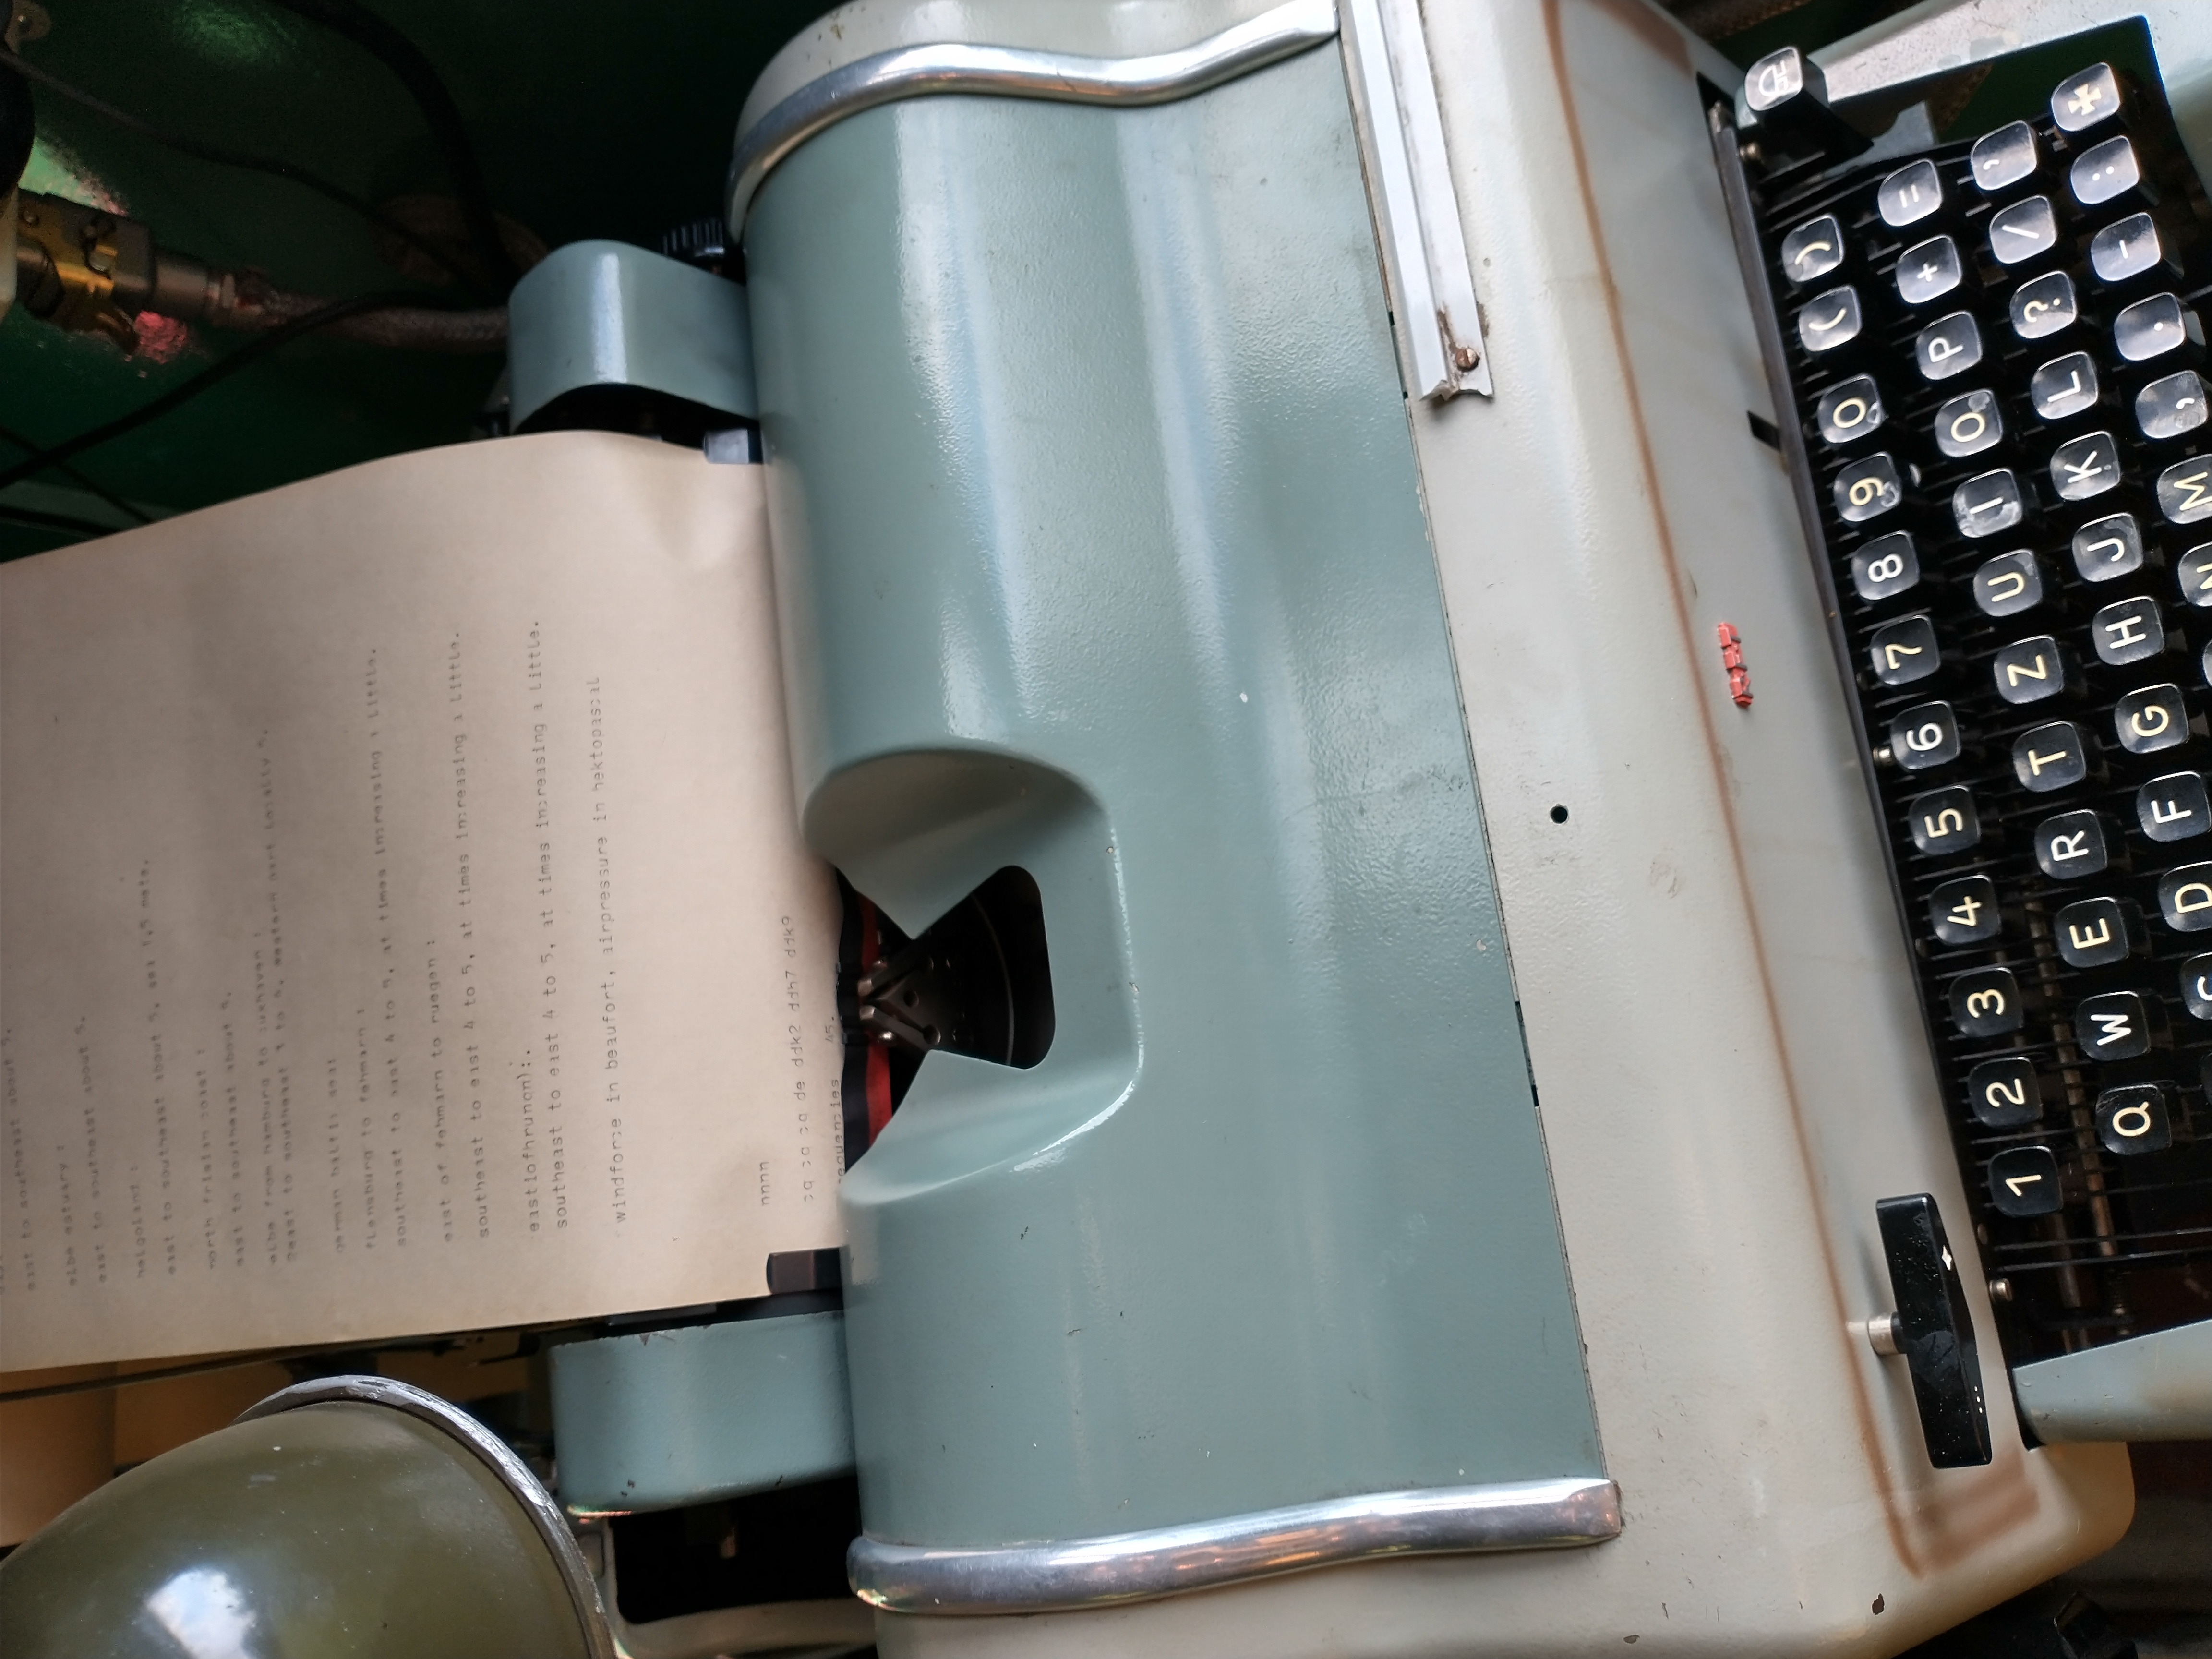
\includegraphics[width=0.85\textwidth]{foto/92}
    \caption{\scriptsize Funkfernschreiber}
    \label{n_computersteuerung_funkfernschreiber}
\end{figure}

    \end{column}
   \begin{column}{0.48\textwidth}
       Die Abkürzung RTTY stammt von \emph{radio teletype}


   \end{column}
\end{columns}

\end{frame}

\begin{frame}
\frametitle{Betrieb}
\begin{columns}
    \begin{column}{0.48\textwidth}
    \begin{itemize}
  \item Beide Funkpartner nutzen das gleiche Übertragungsverfahren (z.B. JS8, PSK, RTTY)
  \item Gleiche Parameter müssen gesetzt sein
  \end{itemize}

    \end{column}
   \begin{column}{0.48\textwidth}
       \begin{itemize}
  \item Verwendung von betrieblichen Abkürzungen und Q-Gruppen
  \item Mehr Informationsgehalt pro Zeiteinheit
  \end{itemize}

   \end{column}
\end{columns}

\end{frame}

\begin{frame}In einem Gespräch sieht dieses folgendermaßen aus:
    \pause\QSOown{CQ CQ CQ DE DL2AB DL2AB DL2AB PSE K}\pause\QSOother{DL2AB DE DL1PZ K}\pause\QSOown{DL1PZ DE DL2AB = UR RST 599 599 = DL1PZ DE DL2AB K}\pause\QSOother{DL2AB DE DL1PZ = TNX RPRT, UR 479 479 BK}\pause\QSOown{BK QSL = VY 73 DE DL2AB SK}\pause\QSOother{R 73 DE DL1PZ SK}

\end{frame}

\begin{frame}
\begin{columns}
    \begin{column}{0.48\textwidth}
    \begin{table}
\begin{DARCtabular}{ll}
     Abkz.  & Bedeutung   \\
     BK  & Unterbrechung der Sendung; Formlose Übergabe   \\
     CQ  & Allgemeiner Anruf (vom Englischen \enquote{Seek You})   \\
     DE  & von   \\
     K  & Aufforderung zum Senden   \\
     PSE  & Bitte (vom Englischen \enquote{Please})   \\
     QSL  & Ich bestätige den Empfang   \\
     R  & Received (Empfangsbestätigung)   \\
     RPRT  & Rapport (vom Englischen \enquote{Report})   \\
\end{DARCtabular}
\caption{Betriebliche Abkürzungen in der Telegrafie}
\label{n_funkfernschreiben_abkuerzungen_1}
\end{table}

    \end{column}
   \begin{column}{0.48\textwidth}
       \begin{table}
\begin{DARCtabular}{ll}
     Abkz.  & Bedeutung   \\
     RST  & RST-Rapport   \\
     SK  & Ende der Verbindung (vom Englischen \enquote{Silent Key})   \\
     TNX  & Danke (vom Englischen \enquote{Thanks})   \\
     UR  & du bist (im Sinne von \enquote{dein Signal ist}, vom Englischen \enquote{you are})   \\
     VY  & sehr (vom Englischen \enquote{very})   \\
     73  & viele Grüße   \\
     =  & Trennzeichen   \\
\end{DARCtabular}
\caption{Betriebliche Abkürzungen in der Telegrafie}
\label{n_funkfernschreiben_abkuerzungen_2}
\end{table}

   \end{column}
\end{columns}

\end{frame}

\begin{frame}Teil 1 unseres Beispiel-Gesprächs:
    \pause\QSOown{CQ CQ CQ DE DL2AB DL2AB DL2AB PSE K}\pause\QSOother{DL2AB DE DL1PZ K}
    \pause
    Allgemeiner Anruf von DL2AB -- Bitte Kommen!
    \pause
    DL2AB von DL1PZ -- Kommen!



\end{frame}

\begin{frame}Teil 2 unseres Beispiel-Gesprächs:
    \pause\QSOown{DL1PZ DE DL2AB = UR RST 599 599 = DL1PZ DE DL2AB K}\pause\QSOother{DL2AB DE DL1PZ = TNX RPRT, UR 479 479 BK}
    \pause
    DL1PZ von DL2AB. Dein Signal ist mit dem RST-Wert 599, ich wiederhole, 599. DL1PZ von DL2AB -- Kommen!
    \pause
    DL2AB von DL1PZ. Danke für den RST-Rapport, dein Signal ist 479, ich wiederhole, 479. Zurück zu dir!



\end{frame}

\begin{frame}Teil 3 unseres Beispiel-Gesprächs:
    \pause\QSOown{BK QSL = VY 73 DE DL2AB SK}\pause\QSOother{R 73 DE DL1PZ SK}
    \pause
    Hier bin ich wieder. Ich bestätige den Empfang. Sehr viele Grüße von DL2AB. Ende der Verbindung.
    \pause
    Verstanden. Viele Grüße von DL1PZ. Ende der Verbindung.



\end{frame}

\begin{frame}
\only<1>{
\begin{QQuestion}{NE401}{Was sollten Sie bei der Übertragung eines Textes per Funkfernschreiben beachten?}{Sende- und Empfangsstation müssen das gleiche Übertragungsverfahren (z. B. JS8, PSK, RTTY) und ggf. die gleichen Verfahrensparameter verwenden.}
{Sende- und Empfangsstation müssen die gleiche Zeitzoneneinstellung (z. B. Sommerzeit) aufweisen, damit die Übertragung erfolgreich sein kann.}
{Die Übertragung sollte bevorzugt während der Abend- und Nachtstunden stattfinden, da die Frequenzen tagsüber für Sprechverbindungen freigehalten werden.}
{Die Übertragung sollte bevorzugt mit einem schnellen Verfahren stattfinden, damit die Amateurfunkbänder nicht unnötig belastet werden.}
\end{QQuestion}

}
\only<2>{
\begin{QQuestion}{NE401}{Was sollten Sie bei der Übertragung eines Textes per Funkfernschreiben beachten?}{\textbf{\textcolor{DARCgreen}{Sende- und Empfangsstation müssen das gleiche Übertragungsverfahren (z. B. JS8, PSK, RTTY) und ggf. die gleichen Verfahrensparameter verwenden.}}}
{Sende- und Empfangsstation müssen die gleiche Zeitzoneneinstellung (z. B. Sommerzeit) aufweisen, damit die Übertragung erfolgreich sein kann.}
{Die Übertragung sollte bevorzugt während der Abend- und Nachtstunden stattfinden, da die Frequenzen tagsüber für Sprechverbindungen freigehalten werden.}
{Die Übertragung sollte bevorzugt mit einem schnellen Verfahren stattfinden, damit die Amateurfunkbänder nicht unnötig belastet werden.}
\end{QQuestion}

}
\end{frame}

\begin{frame}
\only<1>{
\begin{QQuestion}{BB101}{Warum werden insbesondere in der Telegrafie (z.~B. CW, JS8, RTTY) betriebliche Abkürzungen und Q-Gruppen verwendet?}{Sie werden als Kennung beim Amateurfunkpeilen genutzt, um die Sender zu kennzeichnen.}
{Der Informationsgehalt einer Aussendung wird verschleiert und ist damit für Unbeteiligte nicht verständlich.}
{Sie werden bei Verbindungen über Amateurfunksatelliten benutzt, um den Dopplereffekt durch kürzere Durchgänge zu vermeiden.}
{Der Betriebsablauf wird vereinfacht und der zu übertragende Informationsgehalt pro Zeiteinheit optimiert.}
\end{QQuestion}

}
\only<2>{
\begin{QQuestion}{BB101}{Warum werden insbesondere in der Telegrafie (z.~B. CW, JS8, RTTY) betriebliche Abkürzungen und Q-Gruppen verwendet?}{Sie werden als Kennung beim Amateurfunkpeilen genutzt, um die Sender zu kennzeichnen.}
{Der Informationsgehalt einer Aussendung wird verschleiert und ist damit für Unbeteiligte nicht verständlich.}
{Sie werden bei Verbindungen über Amateurfunksatelliten benutzt, um den Dopplereffekt durch kürzere Durchgänge zu vermeiden.}
{\textbf{\textcolor{DARCgreen}{Der Betriebsablauf wird vereinfacht und der zu übertragende Informationsgehalt pro Zeiteinheit optimiert.}}}
\end{QQuestion}

}
\end{frame}

\begin{frame}
\only<1>{
\begin{QQuestion}{BB110}{Was bedeutet \glqq R\grqq{} am Anfang eines Durchgangs in Telegrafie?}{Repeat (wiederhole)}
{Received (empfangen)}
{Rapport (Bericht)}
{Readability (Lesbarkeit)}
\end{QQuestion}

}
\only<2>{
\begin{QQuestion}{BB110}{Was bedeutet \glqq R\grqq{} am Anfang eines Durchgangs in Telegrafie?}{Repeat (wiederhole)}
{\textbf{\textcolor{DARCgreen}{Received (empfangen)}}}
{Rapport (Bericht)}
{Readability (Lesbarkeit)}
\end{QQuestion}

}
\end{frame}

\begin{frame}
\only<1>{
\begin{QQuestion}{BB109}{Was bedeutet \glqq K\grqq{} am Ende eines Durchgangs in Telegrafie?}{Unterbrechung der Sendung}
{Aufforderung zum Senden}
{Bitte warten}
{Beendigung des Funkverkehrs}
\end{QQuestion}

}
\only<2>{
\begin{QQuestion}{BB109}{Was bedeutet \glqq K\grqq{} am Ende eines Durchgangs in Telegrafie?}{Unterbrechung der Sendung}
{\textbf{\textcolor{DARCgreen}{Aufforderung zum Senden}}}
{Bitte warten}
{Beendigung des Funkverkehrs}
\end{QQuestion}

}
\end{frame}

\begin{frame}
\only<1>{
\begin{QQuestion}{BB108}{Was bedeutet die Betriebsabkürzung \glqq BK\grqq{} in Telegrafie?}{Beendigung des Funkverkehrs; wird auch zur formlosen Begrüßung genutzt}
{Alles richtig verstanden; wird auch zur schnellen Beendigung eines Funkkontakts genutzt}
{Bitte warten; wird auch zur schnellen Anforderung eines Rapports genutzt}
{Signal zur Unterbrechung einer laufenden Sendung; wird auch zur formlosen Übergabe genutzt}
\end{QQuestion}

}
\only<2>{
\begin{QQuestion}{BB108}{Was bedeutet die Betriebsabkürzung \glqq BK\grqq{} in Telegrafie?}{Beendigung des Funkverkehrs; wird auch zur formlosen Begrüßung genutzt}
{Alles richtig verstanden; wird auch zur schnellen Beendigung eines Funkkontakts genutzt}
{Bitte warten; wird auch zur schnellen Anforderung eines Rapports genutzt}
{\textbf{\textcolor{DARCgreen}{Signal zur Unterbrechung einer laufenden Sendung; wird auch zur formlosen Übergabe genutzt}}}
\end{QQuestion}

}
\end{frame}

\begin{frame}
\only<1>{
\begin{QQuestion}{BE112}{Wie gestalten Sie beispielsweise als \glqq DL2AB\grqq{} einen allgemeinen Anruf in Telegrafie?}{CQ CQ CQ DE DL2AB DL2AB DL2AB pse k}
{CQ CQ CQ FRM DL2AB DL2AB DL2AB pse k}
{QRZ QRZ QRZ DE DL2AB DL2AB DL2AB pse k}
{CQ QRZ CQ QRZ CQ QRZ DE DL2AB DL2AB DL2AB pse k}
\end{QQuestion}

}
\only<2>{
\begin{QQuestion}{BE112}{Wie gestalten Sie beispielsweise als \glqq DL2AB\grqq{} einen allgemeinen Anruf in Telegrafie?}{\textbf{\textcolor{DARCgreen}{CQ CQ CQ DE DL2AB DL2AB DL2AB pse k}}}
{CQ CQ CQ FRM DL2AB DL2AB DL2AB pse k}
{QRZ QRZ QRZ DE DL2AB DL2AB DL2AB pse k}
{CQ QRZ CQ QRZ CQ QRZ DE DL2AB DL2AB DL2AB pse k}
\end{QQuestion}

}
\end{frame}

\begin{frame}
\frametitle{Morsetelegrafie}
\begin{itemize}
  \item Auf die richtige Geschwindigkeit achten
  \item Schnell gegebene Morsezeichen brauchen viel Übung zum Verstehen
  \item Gegenstelle nicht mit der Geschwindigkeit überfordern
  \item Faustregel: \emph{Nicht schneller geben, als man selbst aufnehmen kann}
  \end{itemize}

\end{frame}

\begin{frame}
\only<1>{
\begin{QQuestion}{BE117}{Mit welcher Geschwindigkeit sollten Sie einen Anruf in Morsetelegrafie beantworten? In der Regel antworte ich~...}{mit einem Gebetempo von maximal 60 CPM.}
{mit meiner gewohnten Geschwindigkeit.}
{genauso schnell oder langsamer als der Anruf.}
{mit dem höchsten Tempo, das ich fehlerfrei geben kann.}
\end{QQuestion}

}
\only<2>{
\begin{QQuestion}{BE117}{Mit welcher Geschwindigkeit sollten Sie einen Anruf in Morsetelegrafie beantworten? In der Regel antworte ich~...}{mit einem Gebetempo von maximal 60 CPM.}
{mit meiner gewohnten Geschwindigkeit.}
{\textbf{\textcolor{DARCgreen}{genauso schnell oder langsamer als der Anruf.}}}
{mit dem höchsten Tempo, das ich fehlerfrei geben kann.}
\end{QQuestion}

}
\end{frame}

\begin{frame}
\only<1>{
\begin{QQuestion}{BE118}{Was sollten Sie hinsichtlich der Geschwindigkeit bei Morsetelegrafie beachten? Ich gebe in der Regel~...}{nicht schneller, als ich auch aufnehmen kann, und passe mich an langsamere Stationen an.}
{im international festgelegten Einheitstempo von 12 WPM, um eine automatische Dekodierung zu ermöglichen.}
{so schnell ich kann, damit es nicht zu unnötigen Verzögerungen im Betriebsablauf kommt.}
{in dem Tempo, das mir am besten liegt. Andere müssen sich an mich anpassen.}
\end{QQuestion}

}
\only<2>{
\begin{QQuestion}{BE118}{Was sollten Sie hinsichtlich der Geschwindigkeit bei Morsetelegrafie beachten? Ich gebe in der Regel~...}{\textbf{\textcolor{DARCgreen}{nicht schneller, als ich auch aufnehmen kann, und passe mich an langsamere Stationen an.}}}
{im international festgelegten Einheitstempo von 12 WPM, um eine automatische Dekodierung zu ermöglichen.}
{so schnell ich kann, damit es nicht zu unnötigen Verzögerungen im Betriebsablauf kommt.}
{in dem Tempo, das mir am besten liegt. Andere müssen sich an mich anpassen.}
\end{QQuestion}

}
\end{frame}%ENDCONTENT


\section{Digital Voice (DV)}
\label{section:digital_voice}
\begin{frame}%STARTCONTENT
\begin{itemize}
  \item Auch Sprache kann digital übertragen werden
  \item z.\,B. mit den Übertragungsverfahren DMR, D-Star, C4FM und M17
  \item Sprachsignale werden vor der Übertragung in einen Datenstrom umgewandelt
  \end{itemize}
\end{frame}

\begin{frame}
\frametitle{TDMA}
Time Division Multiple Access -- Zeitmultiplexverfahren
\begin{columns}
    \begin{column}{0.48\textwidth}
    \begin{itemize}
  \item Übertragung mehrerer Datenströme in schnell abwechselnder Folge
  \item Zwei oder mehr Sprachverbindungen nutzen quasi gleichzeitig dieselbe Frequenz
  \end{itemize}

    \end{column}
   \begin{column}{0.48\textwidth}
       
\begin{figure}
    \DARCimage{0.85\linewidth}{474include}
    \caption{\scriptsize TDMA mit drei Verbindungen auf einer Frequenz}
    \label{n_digital_voice_tdma}
\end{figure}


   \end{column}
\end{columns}

\end{frame}

\begin{frame}
\frametitle{Einstellungen}
Es sind für digitale Sprache oft mehr Einstellungen zu berücksichtigen als zum Beispiel bei einer FM-Verbindung. Zum Beispiel:

\begin{itemize}
  \item Sprechgruppe (Talkgroup)
  \item Raum oder Reflektor zum Zusammenschalten von Relaisfunkstellen
  \item TDMA-Zeitschlitz
  \item Color-Code
  \end{itemize}
\end{frame}

\begin{frame} 
\only<1>{
\begin{QQuestion}{NE404}{Welche Übertragungsverfahren für digitalen Sprechfunk sind im Amateurfunk gebräuchlich?}{FM-Sprechfunk, RTTY, D-STAR, JS8, Olivia}
{AM-Sprechfunk, FM-Sprechfunk, SSB-Sprechfunk, Olivia, SSTV}
{DMR, D-STAR, C4FM, M17, FreeDV}
{SSB-Sprechfunk, FT8, DMR, PSK31, SSTV}
\end{QQuestion}

}
\only<2>{
\begin{QQuestion}{NE404}{Welche Übertragungsverfahren für digitalen Sprechfunk sind im Amateurfunk gebräuchlich?}{FM-Sprechfunk, RTTY, D-STAR, JS8, Olivia}
{AM-Sprechfunk, FM-Sprechfunk, SSB-Sprechfunk, Olivia, SSTV}
{\textbf{\textcolor{DARCgreen}{DMR, D-STAR, C4FM, M17, FreeDV}}}
{SSB-Sprechfunk, FT8, DMR, PSK31, SSTV}
\end{QQuestion}

}
\end{frame}

\begin{frame} 
\only<1>{
\begin{QQuestion}{NE307}{Welche Übertragungsverfahren werden bei VHF/UHF-Handfunkgeräten üblicherweise verwendet?}{CW-Morsetelegrafie, FT8, D-STAR}
{FM-Sprechfunk, DMR, D-STAR}
{SSB-Sprechfunk, DMR, RTTY}
{AM-Sprechfunk, C4FM, FT8}
\end{QQuestion}

}
\only<2>{
\begin{QQuestion}{NE307}{Welche Übertragungsverfahren werden bei VHF/UHF-Handfunkgeräten üblicherweise verwendet?}{CW-Morsetelegrafie, FT8, D-STAR}
{\textbf{\textcolor{DARCgreen}{FM-Sprechfunk, DMR, D-STAR}}}
{SSB-Sprechfunk, DMR, RTTY}
{AM-Sprechfunk, C4FM, FT8}
\end{QQuestion}

}
\end{frame}

\begin{frame} 
\only<1>{
\begin{QQuestion}{NE403}{Ist es bei bestimmten digitalen Verfahren zur Sprachübertragung (z.~B. DMR oder TETRA) möglich, mehrere Sprechverbindungen gleichzeitig auf derselben Frequenz innerhalb eines Empfangsgebiets abzuwickeln?}{Nein. Sprachübertragungen können nicht in Datenpakete aufgeteilt werden.}
{Ja. Die Sendeleistung wird zur Verbesserung der digitalen Fehlerkorrektur erhöht.}
{Nein. Zeitgleich stattfindende digitale Übertragungen stören sich prinzipbedingt gegenseitig.}
{Ja. Die Sprachdaten werden abwechselnd in periodischen, kurzen Zeitschlitzen übertragen.}
\end{QQuestion}

}
\only<2>{
\begin{QQuestion}{NE403}{Ist es bei bestimmten digitalen Verfahren zur Sprachübertragung (z.~B. DMR oder TETRA) möglich, mehrere Sprechverbindungen gleichzeitig auf derselben Frequenz innerhalb eines Empfangsgebiets abzuwickeln?}{Nein. Sprachübertragungen können nicht in Datenpakete aufgeteilt werden.}
{Ja. Die Sendeleistung wird zur Verbesserung der digitalen Fehlerkorrektur erhöht.}
{Nein. Zeitgleich stattfindende digitale Übertragungen stören sich prinzipbedingt gegenseitig.}
{\textbf{\textcolor{DARCgreen}{Ja. Die Sprachdaten werden abwechselnd in periodischen, kurzen Zeitschlitzen übertragen.}}}
\end{QQuestion}

}
\end{frame}

\begin{frame} 
\only<1>{
\begin{QQuestion}{NE402}{Sie möchten an einer Funkrunde mittels digitaler Sprachübertragung (z.~B. C4FM, DMR oder D-Star) über ein Repeaternetzwerk teilnehmen. Worauf müssen Sie neben der Wahl des Übertragungsverfahrens, der Frequenz und der Modulation achten?}{Alle Stationen müssen sich in Funkreichweite desselben Repeaters befinden.}
{Sie müssen die gleiche Firmwareversion wie das Repeaternetzwerk verwenden.}
{Alle Stationen müssen die gleiche Stationskennung, z.~B. DMR-ID, einstellen.}
{Sie müssen geeignete Parameter, z.~B. Reflektor, Zeitschlitz oder Color-Code, wählen.}
\end{QQuestion}

}
\only<2>{
\begin{QQuestion}{NE402}{Sie möchten an einer Funkrunde mittels digitaler Sprachübertragung (z.~B. C4FM, DMR oder D-Star) über ein Repeaternetzwerk teilnehmen. Worauf müssen Sie neben der Wahl des Übertragungsverfahrens, der Frequenz und der Modulation achten?}{Alle Stationen müssen sich in Funkreichweite desselben Repeaters befinden.}
{Sie müssen die gleiche Firmwareversion wie das Repeaternetzwerk verwenden.}
{Alle Stationen müssen die gleiche Stationskennung, z.~B. DMR-ID, einstellen.}
{\textbf{\textcolor{DARCgreen}{Sie müssen geeignete Parameter, z.~B. Reflektor, Zeitschlitz oder Color-Code, wählen.}}}
\end{QQuestion}

}
\end{frame}%ENDCONTENT


\title{DARC Amateurfunklehrgang Klasse N}
\author{Abkürzungen}
\institute{Deutscher Amateur Radio Club e.\,V.}
\begin{frame}
\maketitle
\end{frame}

\section{Betriebliche Abkürzungen}
\label{section:betriebliche_abkuerzungen}
\begin{frame}%STARTCONTENT
\begin{table}
\begin{DARCtabular}{cX}
     Abkürzung  & Bedeutung   \\
     BK  & Unterbrechung der Sendung; Formlose Übergabe (\emph{B}rea\emph{k})   \\
     CQ  & Allgemeiner Anruf (vom Englischen \enquote{Seek You})   \\
     CW  & \emph{C}ontinuous \emph{W}ave (Synonym für Morsetelegraphie)   \\
     K  & Aufforderung zum Senden (\enquote{\emph{K}ommen})   \\
     PSE  & Bitte, \emph{P}lea\emph{se}   \\
     R  & Received (Empfangsbestätigung, \emph{R}oger)   \\
     RX  & Receiver (Empfänger)   \\
     TX  & Transmitter (Sender)   \\
     TRX  & Transceiver (Sendeempfänger)   \\
\end{DARCtabular}
\caption{Zusammenfassung der Abkürzungen}
\label{n_abkuerzungen}
\end{table}

\end{frame}

\begin{frame}
\only<1>{
\begin{QQuestion}{BB106}{Was bedeuten die Abkürzungen \glqq TX\grqq{}, \glqq RX\grqq{}, \glqq TRX\grqq{} in dieser Reihenfolge?}{Sender, Empfänger, Sendeempfänger }
{Sendeempfänger, Empfänger, Sender}
{Tonqualität, Lesbarkeit, Signalstärke}
{Signalstärke, Lesbarkeit, Tonqualität}
\end{QQuestion}

}
\only<2>{
\begin{QQuestion}{BB106}{Was bedeuten die Abkürzungen \glqq TX\grqq{}, \glqq RX\grqq{}, \glqq TRX\grqq{} in dieser Reihenfolge?}{\textbf{\textcolor{DARCgreen}{Sender, Empfänger, Sendeempfänger }}}
{Sendeempfänger, Empfänger, Sender}
{Tonqualität, Lesbarkeit, Signalstärke}
{Signalstärke, Lesbarkeit, Tonqualität}
\end{QQuestion}

}
\end{frame}

\begin{frame}
\only<1>{
\begin{QQuestion}{BB107}{Was bedeutet die Abkürzung \glqq CW\grqq{} im Amateurfunk?}{Contestwertung}
{Codewort}
{Calling Wide}
{Continuous Wave}
\end{QQuestion}

}
\only<2>{
\begin{QQuestion}{BB107}{Was bedeutet die Abkürzung \glqq CW\grqq{} im Amateurfunk?}{Contestwertung}
{Codewort}
{Calling Wide}
{\textbf{\textcolor{DARCgreen}{Continuous Wave}}}
\end{QQuestion}

}
\end{frame}

\begin{frame}
\only<1>{
\begin{QQuestion}{BB110}{Was bedeutet \glqq R\grqq{} am Anfang eines Durchgangs in Telegrafie?}{Repeat (wiederhole)}
{Received (empfangen)}
{Rapport (Bericht)}
{Readability (Lesbarkeit)}
\end{QQuestion}

}
\only<2>{
\begin{QQuestion}{BB110}{Was bedeutet \glqq R\grqq{} am Anfang eines Durchgangs in Telegrafie?}{Repeat (wiederhole)}
{\textbf{\textcolor{DARCgreen}{Received (empfangen)}}}
{Rapport (Bericht)}
{Readability (Lesbarkeit)}
\end{QQuestion}

}
\end{frame}

\begin{frame}
\only<1>{
\begin{QQuestion}{BB109}{Was bedeutet \glqq K\grqq{} am Ende eines Durchgangs in Telegrafie?}{Unterbrechung der Sendung}
{Aufforderung zum Senden}
{Bitte warten}
{Beendigung des Funkverkehrs}
\end{QQuestion}

}
\only<2>{
\begin{QQuestion}{BB109}{Was bedeutet \glqq K\grqq{} am Ende eines Durchgangs in Telegrafie?}{Unterbrechung der Sendung}
{\textbf{\textcolor{DARCgreen}{Aufforderung zum Senden}}}
{Bitte warten}
{Beendigung des Funkverkehrs}
\end{QQuestion}

}
\end{frame}

\begin{frame}
\only<1>{
\begin{QQuestion}{BB108}{Was bedeutet die Betriebsabkürzung \glqq BK\grqq{} in Telegrafie?}{Beendigung des Funkverkehrs; wird auch zur formlosen Begrüßung genutzt}
{Alles richtig verstanden; wird auch zur schnellen Beendigung eines Funkkontakts genutzt}
{Bitte warten; wird auch zur schnellen Anforderung eines Rapports genutzt}
{Signal zur Unterbrechung einer laufenden Sendung; wird auch zur formlosen Übergabe genutzt}
\end{QQuestion}

}
\only<2>{
\begin{QQuestion}{BB108}{Was bedeutet die Betriebsabkürzung \glqq BK\grqq{} in Telegrafie?}{Beendigung des Funkverkehrs; wird auch zur formlosen Begrüßung genutzt}
{Alles richtig verstanden; wird auch zur schnellen Beendigung eines Funkkontakts genutzt}
{Bitte warten; wird auch zur schnellen Anforderung eines Rapports genutzt}
{\textbf{\textcolor{DARCgreen}{Signal zur Unterbrechung einer laufenden Sendung; wird auch zur formlosen Übergabe genutzt}}}
\end{QQuestion}

}
\end{frame}%ENDCONTENT


\section{Q-Schlüssel}
\label{section:q_schluessel}
\begin{frame}%STARTCONTENT

\frametitle{Q-Gruppen}
\begin{columns}
    \begin{column}{0.48\textwidth}
    \begin{itemize}
  \item In Radio Regulations (RR) definiert
  \item 3 Zeichen lang
  \item Nutzung als Frage, Antwort oder Aufforderung
  \end{itemize}

    \end{column}
   \begin{column}{0.48\textwidth}
       
    \pause
    Wird ein Fragezeichen angehangen, wird aus einer Aussage eine Frage:

QTH Berlin $\rightarrow$ QTH?




   \end{column}
\end{columns}

\end{frame}

\begin{frame}
\only<1>{
\begin{QQuestion}{VA407}{In welchem internationalen Regelwerk können die Bedeutungen der im Amateurfunk gebräuchlichen Q-Gruppen nachgeschlagen werden? In den~...}{Empfehlungen der Internationalen Organisation für Normung (ISO)}
{Empfehlungen der International Amateur Radio Union (IARU)}
{Standards des European Telecommunications Standards Institute (ETSI)}
{Radio Regulations (RR)}
\end{QQuestion}

}
\only<2>{
\begin{QQuestion}{VA407}{In welchem internationalen Regelwerk können die Bedeutungen der im Amateurfunk gebräuchlichen Q-Gruppen nachgeschlagen werden? In den~...}{Empfehlungen der Internationalen Organisation für Normung (ISO)}
{Empfehlungen der International Amateur Radio Union (IARU)}
{Standards des European Telecommunications Standards Institute (ETSI)}
{\textbf{\textcolor{DARCgreen}{Radio Regulations (RR)}}}
\end{QQuestion}

}
\end{frame}

\begin{frame}\begin{table}
\begin{DARCtabular}{lll}
      & Bedeutung  & Merkhilfe   \\
     QRN  & Atmosphärische Störungen  & \emph{N}atürliche Störung   \\
     QRM  & Ich werde gestört  & \emph{M}enschengemachte Störung   \\
     QRO  & Erhöhen Sie die Sendeleistung!  & Ein paar Watt \emph{o}bendrauf legen   \\
     QRP  & Senken Sie die Sendeleistung!  & \emph{P}iano (sanft, leise), \emph{P}ssst!  \\
     QRT  & Stellen Sie die Übermittlung ein!  & \emph{T}erminal (Ende)   \\
     QRV  & Ich bin bereit  & \emph{v}orbereitet   \\
\end{DARCtabular}
\caption{Alle prüfungsrelevanten Q-Gruppen in der Übersicht mit Merkhilfen}
\label{n_q_gruppen_1}
\end{table}

\end{frame}

\begin{frame}\begin{table}
\begin{DARCtabular}{lll}
      & Bedeutung  & Merkhilfe   \\
     QRX?  & Wann rufen Sie mich wieder?  & Zeitpunkt \emph{X}   \\
     QRZ?  & Wer hat mich gerufen?  & Bitte nenne das Rufzeichen ein \emph{z}weites Mal!   \\
     QSB  & Fading, Schwankungen  & \emph{B}ergauf, \emph{B}ergab   \\
     QSL  & Ich bestätige den Empfang  & Ich habe ge\emph{l}oggt   \\
     QSO?  & Erreichen Sie Station~...~?  &    \\
     QSY  & Frequenzwechsel  & Change Frequenc\emph{y}   \\
     QTH  & Mein Standort  & \emph{H}ome, \emph{H}eimat   \\
\end{DARCtabular}
\caption{Alle prüfungsrelevanten Q-Gruppen in der Übersicht mit Merkhilfen}
\label{n_q_gruppen_2}
\end{table}

\end{frame}

\begin{frame}
\only<1>{
\begin{QQuestion}{BB204}{Was bedeuten die Q-Gruppen \glqq QRV\grqq{}, \glqq QRM?\grqq{} und \glqq QTH\grqq{}?}{Ich habe nichts mehr für Sie. Werden Sie gestört? Mein Standort ist...}
{Senden Sie eine Reihe V. Soll ich mehr Sendeleistung anwenden? Ihre gesendeten Töne sind kaum hörbar.}
{Ich bin bereit. Werden Sie gestört? Mein Standort ist...}
{Ich habe nichts mehr für Sie. Mein Standort ist... Ich bin bereit.}
\end{QQuestion}

}
\only<2>{
\begin{QQuestion}{BB204}{Was bedeuten die Q-Gruppen \glqq QRV\grqq{}, \glqq QRM?\grqq{} und \glqq QTH\grqq{}?}{Ich habe nichts mehr für Sie. Werden Sie gestört? Mein Standort ist...}
{Senden Sie eine Reihe V. Soll ich mehr Sendeleistung anwenden? Ihre gesendeten Töne sind kaum hörbar.}
{\textbf{\textcolor{DARCgreen}{Ich bin bereit. Werden Sie gestört? Mein Standort ist...}}}
{Ich habe nichts mehr für Sie. Mein Standort ist... Ich bin bereit.}
\end{QQuestion}

}
\end{frame}

\begin{frame}
\only<1>{
\begin{QQuestion}{BB203}{Was bedeuten die Q-Gruppen \glqq QRT\grqq{}, \glqq QRZ?\grqq{} und \glqq QSL?\grqq{}?}{Ich habe nichts für Sie. Von wem werde ich gerufen? Können Sie den Empfang bestätigen??}
{Stellen Sie die Übermittlung ein. Ich bin bereit. Schicken Sie eine QSL-Karte?}
{Stellen Sie die Übermittlung ein. Wie ist Ihr Standort? Können Sie den Empfang bestätigen??}
{Stellen Sie die Übermittlung ein. Von wem werde ich gerufen? Können Sie den Empfang bestätigen??}
\end{QQuestion}

}
\only<2>{
\begin{QQuestion}{BB203}{Was bedeuten die Q-Gruppen \glqq QRT\grqq{}, \glqq QRZ?\grqq{} und \glqq QSL?\grqq{}?}{Ich habe nichts für Sie. Von wem werde ich gerufen? Können Sie den Empfang bestätigen??}
{Stellen Sie die Übermittlung ein. Ich bin bereit. Schicken Sie eine QSL-Karte?}
{Stellen Sie die Übermittlung ein. Wie ist Ihr Standort? Können Sie den Empfang bestätigen??}
{\textbf{\textcolor{DARCgreen}{Stellen Sie die Übermittlung ein. Von wem werde ich gerufen? Können Sie den Empfang bestätigen??}}}
\end{QQuestion}

}
\end{frame}

\begin{frame}
\only<1>{
\begin{QQuestion}{BE115}{Was bedeutet die Betriebsabkürzung \glqq QRZ?\grqq{} im Amateurfunk?}{Von wem werde ich gerufen? In Pile-Ups auch: Aufruf weiterer Stationen}
{Sind Sie bereit? Im Contest auch: Alles aufgenommen?}
{Wie ist Ihr Standort? Im Contest auch: Wie ist Ihre Entfernung?}
{Können Sie den Empfang bestätigen? In Pile-Ups auch: Aufforderung zum Rapport}
\end{QQuestion}

}
\only<2>{
\begin{QQuestion}{BE115}{Was bedeutet die Betriebsabkürzung \glqq QRZ?\grqq{} im Amateurfunk?}{\textbf{\textcolor{DARCgreen}{Von wem werde ich gerufen? In Pile-Ups auch: Aufruf weiterer Stationen}}}
{Sind Sie bereit? Im Contest auch: Alles aufgenommen?}
{Wie ist Ihr Standort? Im Contest auch: Wie ist Ihre Entfernung?}
{Können Sie den Empfang bestätigen? In Pile-Ups auch: Aufforderung zum Rapport}
\end{QQuestion}

}
\end{frame}

\begin{frame}
\only<1>{
\begin{QQuestion}{BB202}{Was bedeuten die Q-Gruppen \glqq QRO?\grqq{}, \glqq QSO?\grqq{} und \glqq QRX?\grqq{}?}{Soll ich die Sendeleistung erhöhen? Können Sie direkt Funkverkehr aufnehmen mit ...? Wann werden Sie mich wieder rufen?}
{Soll ich meine Sendeleistung erhöhen? Haben Sie noch etwas für mich vorliegen? Werden Sie mich wieder rufen?}
{Soll ich die Sendeleistung verringern? Haben Sie noch etwas für mich vorliegen? Können Sie direkt Funkverkehr aufnehmen mit ...?}
{Haben Sie noch etwas für mich vorliegen? Können Sie direkt Funkverkehr aufnehmen mit ...? Wann werden Sie mich wieder rufen?}
\end{QQuestion}

}
\only<2>{
\begin{QQuestion}{BB202}{Was bedeuten die Q-Gruppen \glqq QRO?\grqq{}, \glqq QSO?\grqq{} und \glqq QRX?\grqq{}?}{\textbf{\textcolor{DARCgreen}{Soll ich die Sendeleistung erhöhen? Können Sie direkt Funkverkehr aufnehmen mit ...? Wann werden Sie mich wieder rufen?}}}
{Soll ich meine Sendeleistung erhöhen? Haben Sie noch etwas für mich vorliegen? Werden Sie mich wieder rufen?}
{Soll ich die Sendeleistung verringern? Haben Sie noch etwas für mich vorliegen? Können Sie direkt Funkverkehr aufnehmen mit ...?}
{Haben Sie noch etwas für mich vorliegen? Können Sie direkt Funkverkehr aufnehmen mit ...? Wann werden Sie mich wieder rufen?}
\end{QQuestion}

}
\end{frame}

\begin{frame}
\only<1>{
\begin{QQuestion}{BB205}{Wie verhalten Sie sich, wenn Sie \glqq PSE QRP\grqq{} aufnehmen?}{Sie senden eine Bestätigungskarte an die Gegenstation.}
{Sie erhöhen die Sendeleistung.}
{Sie wechseln die Frequenz.}
{Sie verringern die Sendeleistung.}
\end{QQuestion}

}
\only<2>{
\begin{QQuestion}{BB205}{Wie verhalten Sie sich, wenn Sie \glqq PSE QRP\grqq{} aufnehmen?}{Sie senden eine Bestätigungskarte an die Gegenstation.}
{Sie erhöhen die Sendeleistung.}
{Sie wechseln die Frequenz.}
{\textbf{\textcolor{DARCgreen}{Sie verringern die Sendeleistung.}}}
\end{QQuestion}

}
\end{frame}

\begin{frame}
\only<1>{
\begin{QQuestion}{BB201}{Was bedeuten die Q-Gruppen \glqq QRM\grqq{}, \glqq QRN\grqq{} und \glqq QSB?\grqq{}?}{Ich werde gestört. Ich habe atmosphärische Störungen. Schwankt die Stärke meiner Zeichen?}
{Ich habe Störungen. Sie haben Schwankungen Ihrer Zeichen. Werden Sie gestört?}
{Ich habe atmosphärische Störungen. Ich werde gestört. Schwankt die Stärke meiner Zeichen?}
{Die Stärke Ihrer Zeichen schwankt. Ich werde gestört. Haben Sie atmosphärische Störungen?}
\end{QQuestion}

}
\only<2>{
\begin{QQuestion}{BB201}{Was bedeuten die Q-Gruppen \glqq QRM\grqq{}, \glqq QRN\grqq{} und \glqq QSB?\grqq{}?}{\textbf{\textcolor{DARCgreen}{Ich werde gestört. Ich habe atmosphärische Störungen. Schwankt die Stärke meiner Zeichen?}}}
{Ich habe Störungen. Sie haben Schwankungen Ihrer Zeichen. Werden Sie gestört?}
{Ich habe atmosphärische Störungen. Ich werde gestört. Schwankt die Stärke meiner Zeichen?}
{Die Stärke Ihrer Zeichen schwankt. Ich werde gestört. Haben Sie atmosphärische Störungen?}
\end{QQuestion}

}
\end{frame}

\begin{frame}
\only<1>{
\begin{QQuestion}{BB206}{Wie verhalten Sie sich, wenn Sie \glqq PSE QSY ...\grqq{} aufnehmen?}{Sie erhöhen die Sendeleistung.}
{Sie wechseln die Frequenz.}
{Sie verringern die Sendeleistung.}
{Sie senden eine Bestätigungskarte an die Gegenstation.}
\end{QQuestion}

}
\only<2>{
\begin{QQuestion}{BB206}{Wie verhalten Sie sich, wenn Sie \glqq PSE QSY ...\grqq{} aufnehmen?}{Sie erhöhen die Sendeleistung.}
{\textbf{\textcolor{DARCgreen}{Sie wechseln die Frequenz.}}}
{Sie verringern die Sendeleistung.}
{Sie senden eine Bestätigungskarte an die Gegenstation.}
\end{QQuestion}

}
\end{frame}

\begin{frame}
\only<1>{
\begin{QQuestion}{BE107}{Sie tätigen einen allgemeinen Anruf in Telefonie auf \qty{145,500}{MHz}. Dieser wird von einer Gegenstation beantwortet. Wie sollten Sie das darauffolgende Funkgespräch fortsetzen? Ich fasse mich kurz und schlage~...}{QSY vor.}
{QRV vor.}
{QSB vor.}
{QRZ vor.}
\end{QQuestion}

}
\only<2>{
\begin{QQuestion}{BE107}{Sie tätigen einen allgemeinen Anruf in Telefonie auf \qty{145,500}{MHz}. Dieser wird von einer Gegenstation beantwortet. Wie sollten Sie das darauffolgende Funkgespräch fortsetzen? Ich fasse mich kurz und schlage~...}{\textbf{\textcolor{DARCgreen}{QSY vor.}}}
{QRV vor.}
{QSB vor.}
{QRZ vor.}
\end{QQuestion}

}
\end{frame}%ENDCONTENT


\section{Maidenhead Locator}
\label{section:locator}
\begin{frame}%STARTCONTENT

\frametitle{Problemstellung}
\begin{itemize}
  \item Standort mitteilen, z.B. für Entfernungsmessungen
  \item Es ist nicht immer eine Stadt in der Nähe
  \item GPS-Koordinaten sind zu lang
  \item Oft ist ein ungefährer Standort ausreichend
  \end{itemize}
\end{frame}

\begin{frame}
\frametitle{Maidenhead-Locator}
\begin{itemize}
  \item Erdoberfläche wird in 18.662.400 Kästchen eingeteilt
  \item Ein Kästchen entspricht in Deutschland grob einer Genauigkeit von 5 x \qty{5}{\kilo\metre}
  \item Diese Kästchen werden Subsquare genannt
  \item Übergeordnet sind Squares und Fields
  \end{itemize}

\end{frame}

\begin{frame}
\begin{figure}
    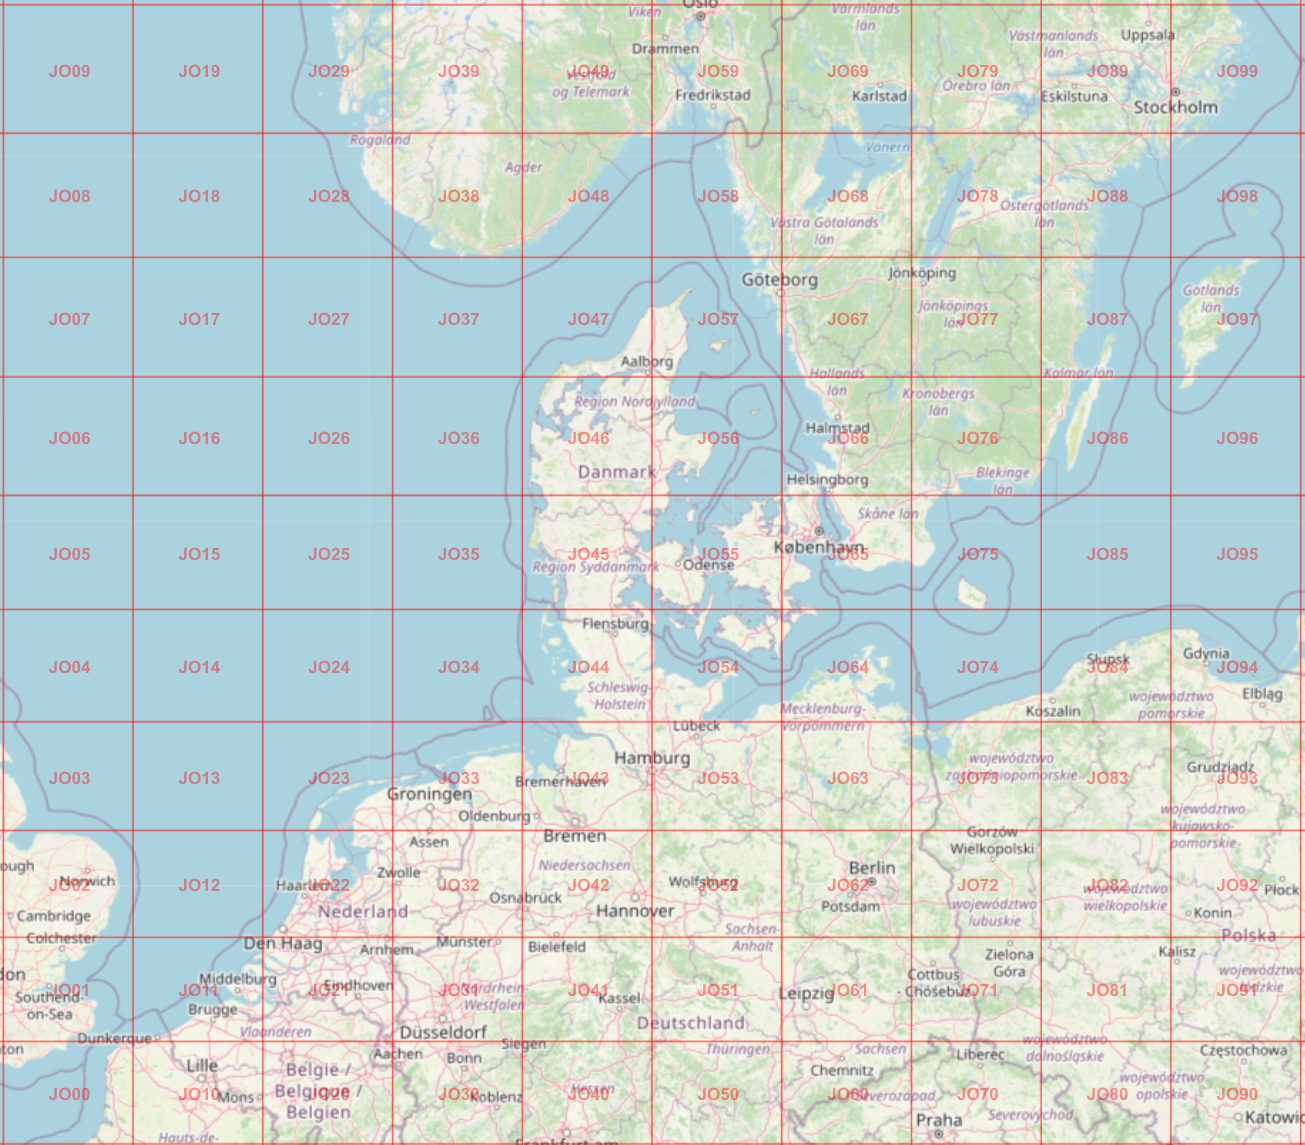
\includegraphics[width=0.85\textwidth]{foto/2}
    \caption{\scriptsize Das Feld JO des Maidenhead-Locator-Systems, Kartendaten © OpenStreetMap-Mitwirkende, SRTM. Kartendarstellung © OpenTopoMap (CC-BY-SA)}
    \label{n_locator_jo}
\end{figure}

\end{frame}

\begin{frame}
\frametitle{Stufen des Maidenhead Locators}
\begin{table}
\begin{DARCtabular}{lllcccc}
     Offizielle Bezeichnung  & Übersetzung  & Alternative Bezeichnung  & & & & Standort DARC   \\
     Field  & Feld  & Größtfeld  & AA  & --  & RR  & JO   \\
     Square  & Quadrat  & Großfeld  & 00  & --  & 99  & 41   \\
     Subsquare  & Unter-Quadrat  & Kleinfeld  & AA  & --  & XX  & RG   \\
\end{DARCtabular}
\caption{Die einzelnen Stufen des Maidenhead-Locators}
\label{n_locator_stufen}
\end{table}
    \pause
    Daraus ergibt sich dann zum Beispiel \emph{JO41RG} für die DARC Geschäftsstelle in Baunatal bei Kassel

\end{frame}

\begin{frame}

\end{frame}

\begin{frame}
\only<1>{
\begin{QQuestion}{BE111}{Was ist der Maidenhead-Locator (auch: QTH-Locator oder Standortkenner)?}{Ein Koordinatensystem, in dem der Standort einer Amateurfunkstelle der zuständigen Behörde mitgeteilt werden muss}
{Eine Positionsangabe durch Verweis auf Felder (fields) und Quadrate (squares), die mit Buchstaben und Ziffern kodiert werden}
{Die Angabe der Standortdaten in Grad, Minuten und Sekunden geographischer Länge und Breite}
{Der geographische Bereich, der sich aus der Zeitzone des Standorts der jeweiligen Amateurfunkstelle ergibt}
\end{QQuestion}

}
\only<2>{
\begin{QQuestion}{BE111}{Was ist der Maidenhead-Locator (auch: QTH-Locator oder Standortkenner)?}{Ein Koordinatensystem, in dem der Standort einer Amateurfunkstelle der zuständigen Behörde mitgeteilt werden muss}
{\textbf{\textcolor{DARCgreen}{Eine Positionsangabe durch Verweis auf Felder (fields) und Quadrate (squares), die mit Buchstaben und Ziffern kodiert werden}}}
{Die Angabe der Standortdaten in Grad, Minuten und Sekunden geographischer Länge und Breite}
{Der geographische Bereich, der sich aus der Zeitzone des Standorts der jeweiligen Amateurfunkstelle ergibt}
\end{QQuestion}

}
\end{frame}%ENDCONTENT


\title{DARC Amateurfunklehrgang Klasse N}
\author{Antennen und Leitungen}
\institute{Deutscher Amateur Radio Club e.\,V.}
\begin{frame}
\maketitle
\end{frame}

\section{Antennen}
\label{section:antennen}
\begin{frame}%STARTCONTENT

\begin{figure}
    \DARCimage{0.85\linewidth}{657include}
    \caption{\scriptsize Schematische Darstellung einer Amateurfunkstation mit Funkgerät, Speiseleitung und Antenne}
    \label{n_trx_kabel_und_antenne}
\end{figure}
\begin{columns}
    \begin{column}{0.48\textwidth}
    \begin{itemize}
  \item Gibt elektrische Schwingungen als Funkwellen ab
  \item Funkwellen breiten sich in der Ferne aus
  \end{itemize}

    \end{column}
   \begin{column}{0.48\textwidth}
       \begin{itemize}
  \item Nimmt beim Empfang Funkwellen auf
  \item Leitet sie als elektrische Schwingungen über das Antennenkabel zum Funkgerät
  \end{itemize}

   \end{column}
\end{columns}

\end{frame}

\begin{frame}
\only<1>{
\begin{PQuestion}{NG101}{Welches Bauteil wird durch das Schaltzeichen symbolisiert?}{Diode}
{Erde}
{Antenne}
{Transistor}
{\DARCimage{0.1\linewidth}{543include}}\end{PQuestion}

}
\only<2>{
\begin{PQuestion}{NG101}{Welches Bauteil wird durch das Schaltzeichen symbolisiert?}{Diode}
{Erde}
{\textbf{\textcolor{DARCgreen}{Antenne}}}
{Transistor}
{\DARCimage{0.1\linewidth}{543include}}\end{PQuestion}

}
\end{frame}%ENDCONTENT


\section{Dipol-Antenne}
\label{section:dipol}
\begin{frame}%STARTCONTENT

\begin{figure}
    \DARCimage{0.85\linewidth}{589include}
    \caption{\scriptsize Darstellung einer Dipol-Antenne}
    \label{n_dipol}
\end{figure}
\begin{columns}
    \begin{column}{0.48\textwidth}
    \begin{itemize}
  \item In der Praxis wird häufig der Halbwellendipol verwendet
  \item Ist eine halbe Wellenlänge lang
  \end{itemize}

    \end{column}
   \begin{column}{0.48\textwidth}
       
    \pause
    Beispiel:

\begin{itemize}
  \item Wellenlänge von \qty{10}{\metre}
  \item halbe Wellenlänge \qty{5}{\metre}
  \item Jedes Teilstück des Dipols \qty{2,5}{\metre}
  \end{itemize}



   \end{column}
\end{columns}

\end{frame}

\begin{frame}
\only<1>{
\begin{PQuestion}{NG103}{Wie wird die dargestellte Antenne bezeichnet?}{Endgespeiste Antenne}
{Groundplane-Antenne}
{Dipol-Antenne}
{Yagi-Uda-Antenne}
{\DARCimage{1.0\linewidth}{589include}}\end{PQuestion}

}
\only<2>{
\begin{PQuestion}{NG103}{Wie wird die dargestellte Antenne bezeichnet?}{Endgespeiste Antenne}
{Groundplane-Antenne}
{\textbf{\textcolor{DARCgreen}{Dipol-Antenne}}}
{Yagi-Uda-Antenne}
{\DARCimage{1.0\linewidth}{589include}}\end{PQuestion}

}
\end{frame}

\begin{frame}
\frametitle{Anpassung}
Dipol-Antenne auf die gewünschte Frequenz bringen durch gleichmäßiges Kürzen oder Verlängern

\begin{itemize}
  \item Zu hohe Resonanzfrequenz: Beide Seiten gleichmäßig verlängern
  \item Zu niedrige Resonanzfrequenz: Beide Seiten gleichmäßig verkürzen
  \end{itemize}
\end{frame}

\begin{frame}
\only<1>{
\begin{QQuestion}{NG304}{Ihre selbstgebaute Dipol-Antenne ist unterhalb der gewünschten Frequenz resonant. Welche Änderung können Sie vornehmen, um die Resonanz in den gewünschten Bereich zu bringen?}{Sendeleistung verringern}
{Beide Enden gleichmäßig verlängern}
{Sendeleistung erhöhen}
{Beide Enden gleichmäßig kürzen}
\end{QQuestion}

}
\only<2>{
\begin{QQuestion}{NG304}{Ihre selbstgebaute Dipol-Antenne ist unterhalb der gewünschten Frequenz resonant. Welche Änderung können Sie vornehmen, um die Resonanz in den gewünschten Bereich zu bringen?}{Sendeleistung verringern}
{Beide Enden gleichmäßig verlängern}
{Sendeleistung erhöhen}
{\textbf{\textcolor{DARCgreen}{Beide Enden gleichmäßig kürzen}}}
\end{QQuestion}

}
\end{frame}

\begin{frame}
\only<1>{
\begin{QQuestion}{NG305}{Ihre selbstgebaute Dipol-Antenne ist oberhalb der gewünschten Frequenz resonant. Welche Änderung können Sie vornehmen, um die Resonanz in den gewünschten Bereich zu bringen?}{Sendeleistung erhöhen}
{Beide Enden gleichmäßig kürzen}
{Beide Enden gleichmäßig verlängern}
{Sendeleistung verringern}
\end{QQuestion}

}
\only<2>{
\begin{QQuestion}{NG305}{Ihre selbstgebaute Dipol-Antenne ist oberhalb der gewünschten Frequenz resonant. Welche Änderung können Sie vornehmen, um die Resonanz in den gewünschten Bereich zu bringen?}{Sendeleistung erhöhen}
{Beide Enden gleichmäßig kürzen}
{\textbf{\textcolor{DARCgreen}{Beide Enden gleichmäßig verlängern}}}
{Sendeleistung verringern}
\end{QQuestion}

}
\end{frame}%ENDCONTENT


\section{Yagi-Uda-Antenne}
\label{section:yagi_uda_1}
\begin{frame}%STARTCONTENT

\begin{columns}
    \begin{column}{0.48\textwidth}
    
\begin{figure}
    \DARCimage{0.85\linewidth}{613include}
    \caption{\scriptsize Yagi-Uda-Antenne mit Einspeisung am Dipol am vorletzten Element}
    \label{n_yagi_uda}
\end{figure}


    \end{column}
   \begin{column}{0.48\textwidth}
       \begin{itemize}
  \item Vor und hinter dem Dipol werden leitende Stäbe geschickt angeordnet
  \item Bündelt Funkwellen in eine bestimmte Richtung
  \end{itemize}

   \end{column}
\end{columns}

\end{frame}

\begin{frame}
\only<1>{
\begin{PQuestion}{NG108}{Wie wird die dargestellte Antenne bezeichnet?}{Dipol-Antenne}
{Yagi-Uda-Antenne}
{Groundplane-Antenne}
{Endgespeiste Antenne}
{\DARCimage{0.5\linewidth}{613include}}\end{PQuestion}

}
\only<2>{
\begin{PQuestion}{NG108}{Wie wird die dargestellte Antenne bezeichnet?}{Dipol-Antenne}
{\textbf{\textcolor{DARCgreen}{Yagi-Uda-Antenne}}}
{Groundplane-Antenne}
{Endgespeiste Antenne}
{\DARCimage{0.5\linewidth}{613include}}\end{PQuestion}

}
\end{frame}%ENDCONTENT


\section{Rundstrahlantennen}
\label{section:rundstrahler}
\begin{frame}%STARTCONTENT
Ein Dipolschenkel wird durch eine Erdung (Ground) oder große Metallfläche (Fahrzeug) ersetzt
\begin{columns}
    \begin{column}{0.48\textwidth}
    
\begin{figure}
    \DARCimage{0.85\linewidth}{669include}
    \caption{\scriptsize Marconi-Antenne}
    \label{n_marconi_antenne}
\end{figure}


    \end{column}
   \begin{column}{0.48\textwidth}
       Erdung kann durch \emph{Radials} ersetzt werden, die eine \emph{Groundplane} bilden


   \end{column}
\end{columns}

\end{frame}

\begin{frame}
\only<1>{
\begin{PQuestion}{NG105}{Wie wird die dargestellte Antenne bezeichnet?}{Groundplane-Antenne}
{Yagi-Uda-Antenne}
{Dipol-Antenne}
{Endgespeiste Antenne}
{\DARCimage{0.5\linewidth}{614include}}\end{PQuestion}

}
\only<2>{
\begin{PQuestion}{NG105}{Wie wird die dargestellte Antenne bezeichnet?}{\textbf{\textcolor{DARCgreen}{Groundplane-Antenne}}}
{Yagi-Uda-Antenne}
{Dipol-Antenne}
{Endgespeiste Antenne}
{\DARCimage{0.5\linewidth}{614include}}\end{PQuestion}

}
\end{frame}

\begin{frame}
\only<1>{
\begin{QQuestion}{NG106}{Die elektrischen Gegengewichte einer Groundplane-Antenne bezeichnet man auch als~...}{Erdelemente.}
{Reflektoren.}
{Direktoren.}
{Radials.}
\end{QQuestion}

}
\only<2>{
\begin{QQuestion}{NG106}{Die elektrischen Gegengewichte einer Groundplane-Antenne bezeichnet man auch als~...}{Erdelemente.}
{Reflektoren.}
{Direktoren.}
{\textbf{\textcolor{DARCgreen}{Radials.}}}
\end{QQuestion}

}
\end{frame}

\begin{frame}
\only<1>{
\begin{QQuestion}{NG104}{Eine Marconi-Antenne ist~...}{eine vertikale Halbwellenantenne.}
{eine 5/8-$\lambda$-Antenne mit abgestimmten Radials.}
{eine horizontale $\lambda$/2-Langdrahtantenne.}
{eine gegen Erde erregte $\lambda$/4-Vertikalantenne.}
\end{QQuestion}

}
\only<2>{
\begin{QQuestion}{NG104}{Eine Marconi-Antenne ist~...}{eine vertikale Halbwellenantenne.}
{eine 5/8-$\lambda$-Antenne mit abgestimmten Radials.}
{eine horizontale $\lambda$/2-Langdrahtantenne.}
{\textbf{\textcolor{DARCgreen}{eine gegen Erde erregte $\lambda$/4-Vertikalantenne.}}}
\end{QQuestion}

}
\end{frame}

\begin{frame}
\only<1>{
\begin{PQuestion}{NG102}{Was wird durch dieses Schaltzeichen symbolisiert?}{Erde}
{Antenne}
{Diode}
{Batterie}
{\DARCimage{0.1\linewidth}{544include}}\end{PQuestion}

}
\only<2>{
\begin{PQuestion}{NG102}{Was wird durch dieses Schaltzeichen symbolisiert?}{\textbf{\textcolor{DARCgreen}{Erde}}}
{Antenne}
{Diode}
{Batterie}
{\DARCimage{0.1\linewidth}{544include}}\end{PQuestion}

}
\end{frame}

\begin{frame}
\only<1>{
\begin{QQuestion}{NG110}{Welche Antenne ist für eine \qty{2}{\m}-QSO-Runde mit im Umkreis verteilten Funkamateuren am besten geeignet?}{Ferritantenne}
{Yagi-Uda-Antenne}
{Rundstrahlantenne}
{Langdrahtantenne}
\end{QQuestion}

}
\only<2>{
\begin{QQuestion}{NG110}{Welche Antenne ist für eine \qty{2}{\m}-QSO-Runde mit im Umkreis verteilten Funkamateuren am besten geeignet?}{Ferritantenne}
{Yagi-Uda-Antenne}
{\textbf{\textcolor{DARCgreen}{Rundstrahlantenne}}}
{Langdrahtantenne}
\end{QQuestion}

}
\end{frame}

\begin{frame}
\only<1>{
\begin{QQuestion}{NG111}{Welche Antennenkonfiguration ist zu wählen, wenn möglichst viele umliegende Relaisstationen im \qty{2}{\m}- oder im \qty{70}{\cm}-Band erreicht werden sollen?}{Eine Ferritantenne auf der Fensterbank.}
{Ein Rundstrahler auf dem Hausdach.}
{Eine in einer Richtung fest montierte horizontale Richtantenne.}
{Eine Magnetfußantenne auf dem Dachboden.}
\end{QQuestion}

}
\only<2>{
\begin{QQuestion}{NG111}{Welche Antennenkonfiguration ist zu wählen, wenn möglichst viele umliegende Relaisstationen im \qty{2}{\m}- oder im \qty{70}{\cm}-Band erreicht werden sollen?}{Eine Ferritantenne auf der Fensterbank.}
{\textbf{\textcolor{DARCgreen}{Ein Rundstrahler auf dem Hausdach.}}}
{Eine in einer Richtung fest montierte horizontale Richtantenne.}
{Eine Magnetfußantenne auf dem Dachboden.}
\end{QQuestion}

}
\end{frame}%ENDCONTENT


\section{Endgespeiste Antennen (End-Fed)}
\label{section:endgespeiste_antennen}
\begin{frame}%STARTCONTENT

\begin{figure}
    \DARCimage{0.85\linewidth}{615include}
    \caption{\scriptsize Schaltbild einer endgespeisten Antenne}
    \label{n_antennenformen_schaltbild_endfed}
\end{figure}

\begin{itemize}
  \item Statt in der Mitte das Antennenkabel an einem Ende des Dipols anschließen
  \item Häufige Bauform: Endgespeister Halbwellendipol
  \item Ist der Draht einer endgespeisten Antenne länger als die Wellenlänge: Langdraht-Antenne
  \end{itemize}
\end{frame}

\begin{frame}
\only<1>{
\begin{PQuestion}{NG107}{Wie wird die dargestellte Antenne bezeichnet?}{Endgespeiste Antenne}
{Groundplane-Antenne}
{Dipol-Antenne}
{Yagi-Uda-Antenne}
{\DARCimage{1.0\linewidth}{615include}}\end{PQuestion}

}
\only<2>{
\begin{PQuestion}{NG107}{Wie wird die dargestellte Antenne bezeichnet?}{\textbf{\textcolor{DARCgreen}{Endgespeiste Antenne}}}
{Groundplane-Antenne}
{Dipol-Antenne}
{Yagi-Uda-Antenne}
{\DARCimage{1.0\linewidth}{615include}}\end{PQuestion}

}
\end{frame}

\begin{frame}
\only<1>{
\begin{QQuestion}{NG109}{Welche Antennenform wird von Funkamateuren in der Regel nur im Kurzwellenbereich und \underline{nicht} im VHF/UHF-Bereich verwendet?}{Langdraht-Antenne}
{Yagi-Uda-Antenne}
{Quad-Antenne}
{Groundplane-Antenne}
\end{QQuestion}

}
\only<2>{
\begin{QQuestion}{NG109}{Welche Antennenform wird von Funkamateuren in der Regel nur im Kurzwellenbereich und \underline{nicht} im VHF/UHF-Bereich verwendet?}{\textbf{\textcolor{DARCgreen}{Langdraht-Antenne}}}
{Yagi-Uda-Antenne}
{Quad-Antenne}
{Groundplane-Antenne}
\end{QQuestion}

}
\end{frame}%ENDCONTENT


\section{Polarisation}
\label{section:polarisation}
\begin{frame}%STARTCONTENT

\begin{columns}
    \begin{column}{0.48\textwidth}
    \begin{itemize}
  \item Polarisation kann \emph{vertikal} oder \emph{horizontal} sein
  \item Lässt sich bei den meisten Antennen leicht erkennen
  \item Auf VHF und höher sollten alle die gleiche Polarisation verwenden
  \end{itemize}

    \end{column}
   \begin{column}{0.48\textwidth}
       \begin{itemize}
  \item \emph{Zirkular} polarisiert
  \item Drehende Funkwellen mit besonderer Antennenbauform
  \item Unterscheidung in \enquote{linkszirkular} und \enquote{rechtszirkular} polarisiert
  \end{itemize}

   \end{column}
\end{columns}

\end{frame}

\begin{frame}
\only<1>{
\begin{QQuestion}{NB304}{Welche Polarisationen unterscheidet man üblicherweise bei der Funkwellenausbreitung im Amateurfunk und wieso sollte man diese beachten?}{Man unterscheidet parallele, koaxiale und drahtlose Polarisation. Die Polarisation der Antennenkabel muss auf die Antennen abgestimmt sein, um Verluste zu minimieren.}
{Man unterscheidet transversale, longitudinale und orthogonale Polarisation. Die Polarisation des Funkgeräts muss an das Stromnetz angepasst sein, um Kurzschlüsse zu vermeiden.}
{Man unterscheidet kohärente, inkohärente und korrelierte Polarisation. Die Polarisation der Funkwellen sollte regelmäßig geändert werden, um die Störfestigkeit zu erhöhen.}
{Man unterscheidet horizontale, vertikale sowie links- und rechtszirkulare Polarisation. Die Polarisation von Sende- und Empfangsantenne sollten angeglichen sein, um eine verlustarme Übertragung zu gewährleisten.}
\end{QQuestion}

}
\only<2>{
\begin{QQuestion}{NB304}{Welche Polarisationen unterscheidet man üblicherweise bei der Funkwellenausbreitung im Amateurfunk und wieso sollte man diese beachten?}{Man unterscheidet parallele, koaxiale und drahtlose Polarisation. Die Polarisation der Antennenkabel muss auf die Antennen abgestimmt sein, um Verluste zu minimieren.}
{Man unterscheidet transversale, longitudinale und orthogonale Polarisation. Die Polarisation des Funkgeräts muss an das Stromnetz angepasst sein, um Kurzschlüsse zu vermeiden.}
{Man unterscheidet kohärente, inkohärente und korrelierte Polarisation. Die Polarisation der Funkwellen sollte regelmäßig geändert werden, um die Störfestigkeit zu erhöhen.}
{\textbf{\textcolor{DARCgreen}{Man unterscheidet horizontale, vertikale sowie links- und rechtszirkulare Polarisation. Die Polarisation von Sende- und Empfangsantenne sollten angeglichen sein, um eine verlustarme Übertragung zu gewährleisten.}}}
\end{QQuestion}

}
\end{frame}%ENDCONTENT


\section{Einbau Kfz}
\label{section:einbau_kfz}
\begin{frame}%STARTCONTENT

\begin{columns}
    \begin{column}{0.48\textwidth}
    
\begin{figure}
    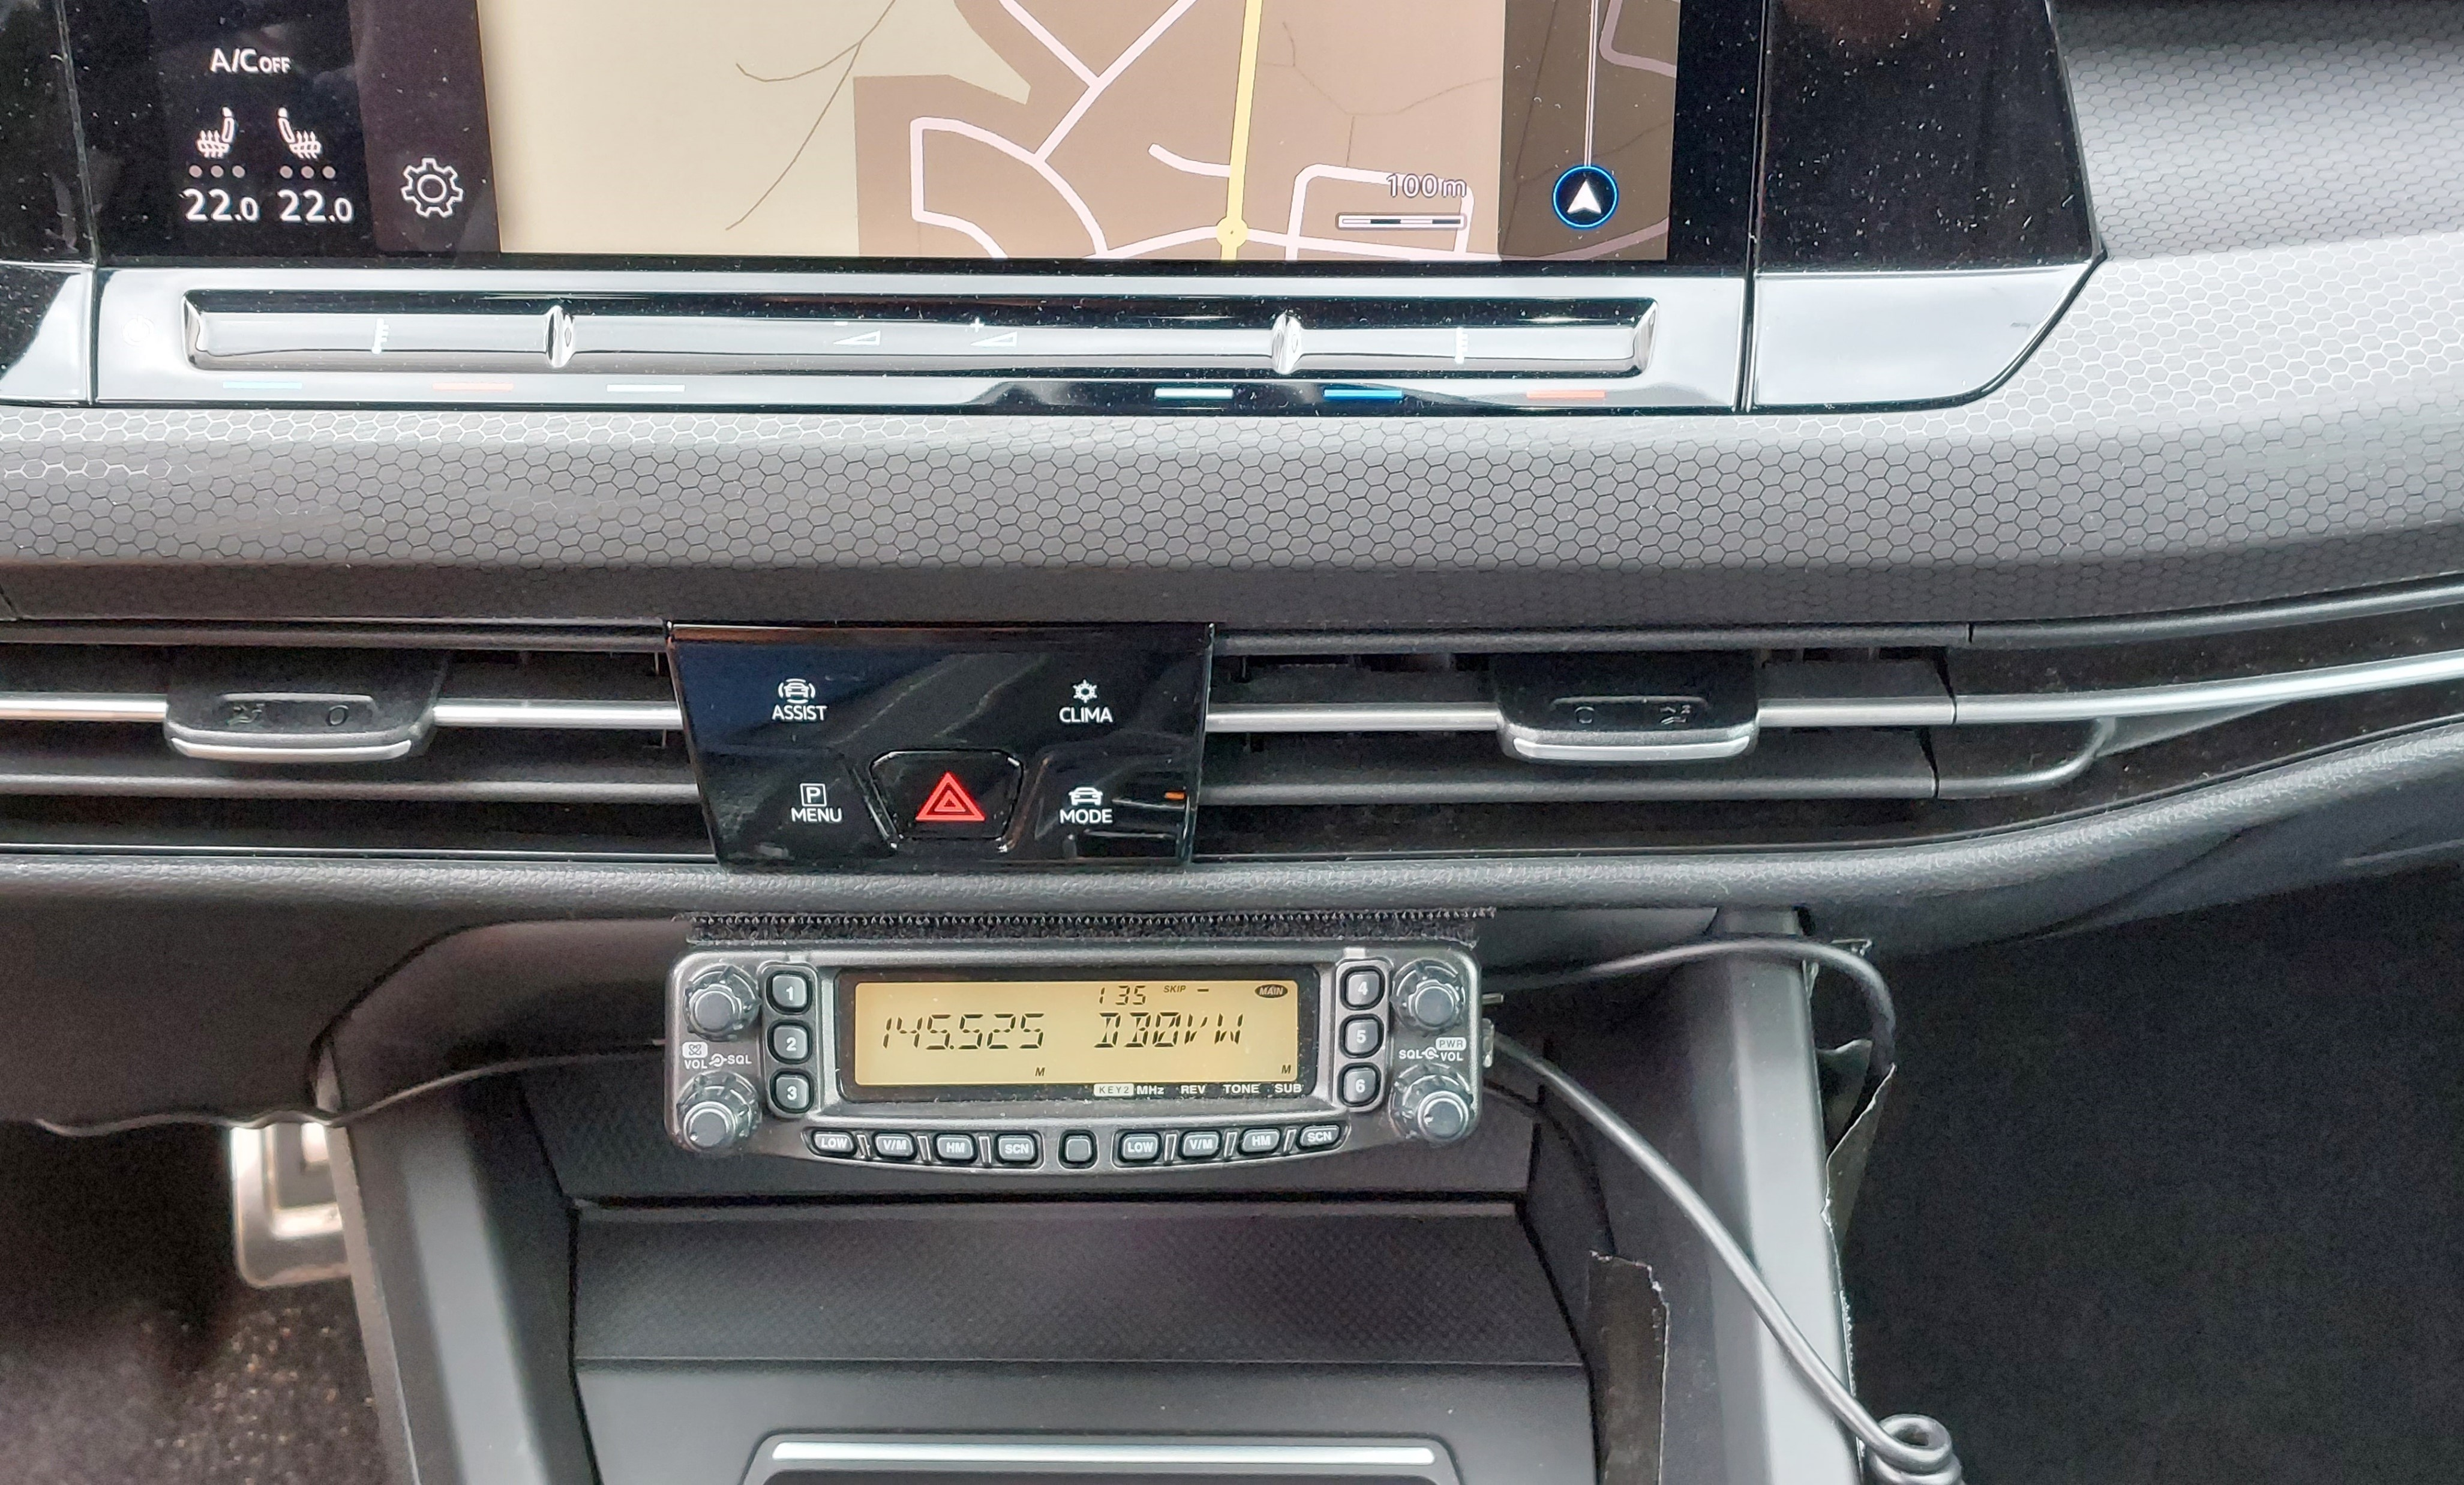
\includegraphics[width=0.85\textwidth]{foto/75}
    \caption{\scriptsize Einbau des Bedienteils eines VHF/UHF-Funkgerätes in die Mittelkonsole eines PKW}
    \label{n_mobilfunkgeraet}
\end{figure}

    \end{column}
   \begin{column}{0.48\textwidth}
       \begin{itemize}
  \item Wähend der Fahrt mit anderen Funkamateuren unterhalten
  \item Tipps oder Verkehrsinformationen mitbekommen
  \item Benutzung nur mit Freisprecheinrichtung
  \end{itemize}

   \end{column}
\end{columns}

\end{frame}

\begin{frame}
\frametitle{Einbau}
\begin{columns}
    \begin{column}{0.48\textwidth}
    
\begin{figure}
    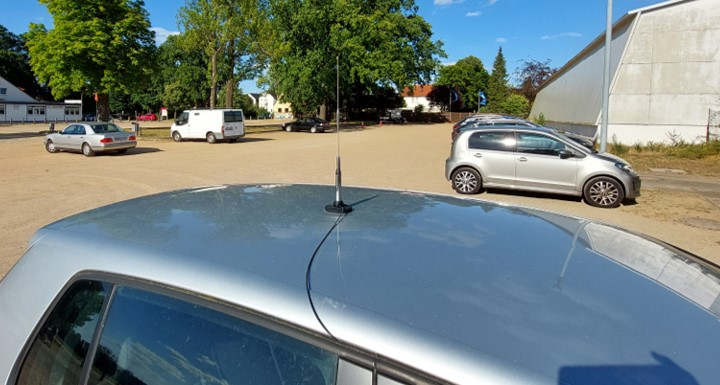
\includegraphics[width=0.85\textwidth]{foto/64}
    \caption{\scriptsize Magnetfußantenne auf Fahrzeugdach}
    \label{n_magnetfussantenne}
\end{figure}
\begin{itemize}
  \item Groundplane-Antenne mit Fahrzeugdach als Gegenelement
  \end{itemize}

    \end{column}
   \begin{column}{0.48\textwidth}
       \begin{itemize}
  \item Möglichst mittig auf dem metallischen Fahrzeugdach
  \item Vorgaben des Fahrzeugherstellers beachten
  \item Leitungen so kurz wie möglich und entfernt von anderen Fahrzeugleitungen
  \end{itemize}

   \end{column}
\end{columns}

\end{frame}

\begin{frame}
\frametitle{Achtung}
\begin{columns}
    \begin{column}{0.48\textwidth}
    
\begin{figure}
    \includegraphics[width=0.85\textwidth]{foto/76}
    \caption{\scriptsize Stromkabel mit Sicherungshalter}
    \label{n_Kabelsicherung}
\end{figure}

    \end{column}
   \begin{column}{0.48\textwidth}
       \begin{itemize}
  \item Bordnetzspannung von \qty{12}{\volt} oder \qty{24}{\volt} scheint ungefährlich
  \item Hohe Ströme sind möglich
  \item Bei Kurzschluss sind Lichtbogen, Kabelbrand oder Fahrzeugbrand möglich
  \item Sicherung des richtigen Werts für das Funkgerät verbauen
  \end{itemize}

   \end{column}
\end{columns}

\end{frame}

\begin{frame}
\only<1>{
\begin{QQuestion}{NK308}{Damit die Zulassung eines Kraftfahrzeugs nicht ungültig wird, sind vor dem Einbau einer mobilen Sende-/Empfangseinrichtung grundsätzlich die Anweisungen~...}{des Amateurfunkgeräte-Herstellers zu beachten.}
{für den Einbau mobiler Sendeanlagen der Bundesnetzagentur einzuhalten.}
{des Kraftfahrt-Bundesamtes einzuhalten.}
{des Kfz-Herstellers zu beachten.}
\end{QQuestion}

}
\only<2>{
\begin{QQuestion}{NK308}{Damit die Zulassung eines Kraftfahrzeugs nicht ungültig wird, sind vor dem Einbau einer mobilen Sende-/Empfangseinrichtung grundsätzlich die Anweisungen~...}{des Amateurfunkgeräte-Herstellers zu beachten.}
{für den Einbau mobiler Sendeanlagen der Bundesnetzagentur einzuhalten.}
{des Kraftfahrt-Bundesamtes einzuhalten.}
{\textbf{\textcolor{DARCgreen}{des Kfz-Herstellers zu beachten.}}}
\end{QQuestion}

}
\end{frame}

\begin{frame}
\only<1>{
\begin{QQuestion}{NK310}{Wo sollte aus funktechnischer Sicht eine mobile VHF-Antenne an einem PKW vorzugsweise installiert werden?}{Auf der hinteren Stoßstange}
{Auf der Mitte des Metalldaches}
{Auf dem vorderen Kotflügel}
{Auf dem Armaturenbrett}
\end{QQuestion}

}
\only<2>{
\begin{QQuestion}{NK310}{Wo sollte aus funktechnischer Sicht eine mobile VHF-Antenne an einem PKW vorzugsweise installiert werden?}{Auf der hinteren Stoßstange}
{\textbf{\textcolor{DARCgreen}{Auf der Mitte des Metalldaches}}}
{Auf dem vorderen Kotflügel}
{Auf dem Armaturenbrett}
\end{QQuestion}

}
\end{frame}

\begin{frame}
\only<1>{
\begin{QQuestion}{NK309}{Um eine Beeinflussung der Elektronik des Kraftfahrzeugs zu verhindern, sollte das Antennenkabel~...}{nicht parallel und möglichst weit von der Fahrzeugverkabelung entfernt verlegt werden.}
{im Kabelbaum des Kraftfahrzeugs geführt werden.}
{über das Fahrzeugdach verlegt sein.}
{entlang der Innenseite des Motorraumes verlegt werden.}
\end{QQuestion}

}
\only<2>{
\begin{QQuestion}{NK309}{Um eine Beeinflussung der Elektronik des Kraftfahrzeugs zu verhindern, sollte das Antennenkabel~...}{\textbf{\textcolor{DARCgreen}{nicht parallel und möglichst weit von der Fahrzeugverkabelung entfernt verlegt werden.}}}
{im Kabelbaum des Kraftfahrzeugs geführt werden.}
{über das Fahrzeugdach verlegt sein.}
{entlang der Innenseite des Motorraumes verlegt werden.}
\end{QQuestion}

}
\end{frame}

\begin{frame}
\only<1>{
\begin{QQuestion}{NK307}{Welche Gefahren können beim unsachgemäßen Anschließen eines Funkgerätes an die \qty{12}{\V}-Batterie in einem Kraftfahrzeug entstehen?}{Überlastung der Sendeendstufe im Funkgerät durch zu hohe Versorgungsspannung}
{Elektrischer Schock durch Überschläge aus der Zündspule}
{Lichtbogen und Fahrzeugbrand}
{Keine, da \qty{12}{\V}-Gleichspannung aus der Kfz-Batterie für den Menschen ungefährlich ist}
\end{QQuestion}

}
\only<2>{
\begin{QQuestion}{NK307}{Welche Gefahren können beim unsachgemäßen Anschließen eines Funkgerätes an die \qty{12}{\V}-Batterie in einem Kraftfahrzeug entstehen?}{Überlastung der Sendeendstufe im Funkgerät durch zu hohe Versorgungsspannung}
{Elektrischer Schock durch Überschläge aus der Zündspule}
{\textbf{\textcolor{DARCgreen}{Lichtbogen und Fahrzeugbrand}}}
{Keine, da \qty{12}{\V}-Gleichspannung aus der Kfz-Batterie für den Menschen ungefährlich ist}
\end{QQuestion}

}
\end{frame}%ENDCONTENT


\section{Übertragungsleitungen}
\label{section:uebertragungsleitungen}
\begin{frame}%STARTCONTENT
Die im Sender erzeugte Sendeleistung möchte man möglichst vollständig und ohne Verluste von der Antenne abstrahlen

\end{frame}

\begin{frame}
\frametitle{Koaxialkabel}
\begin{columns}
    \begin{column}{0.48\textwidth}
    
\begin{figure}
    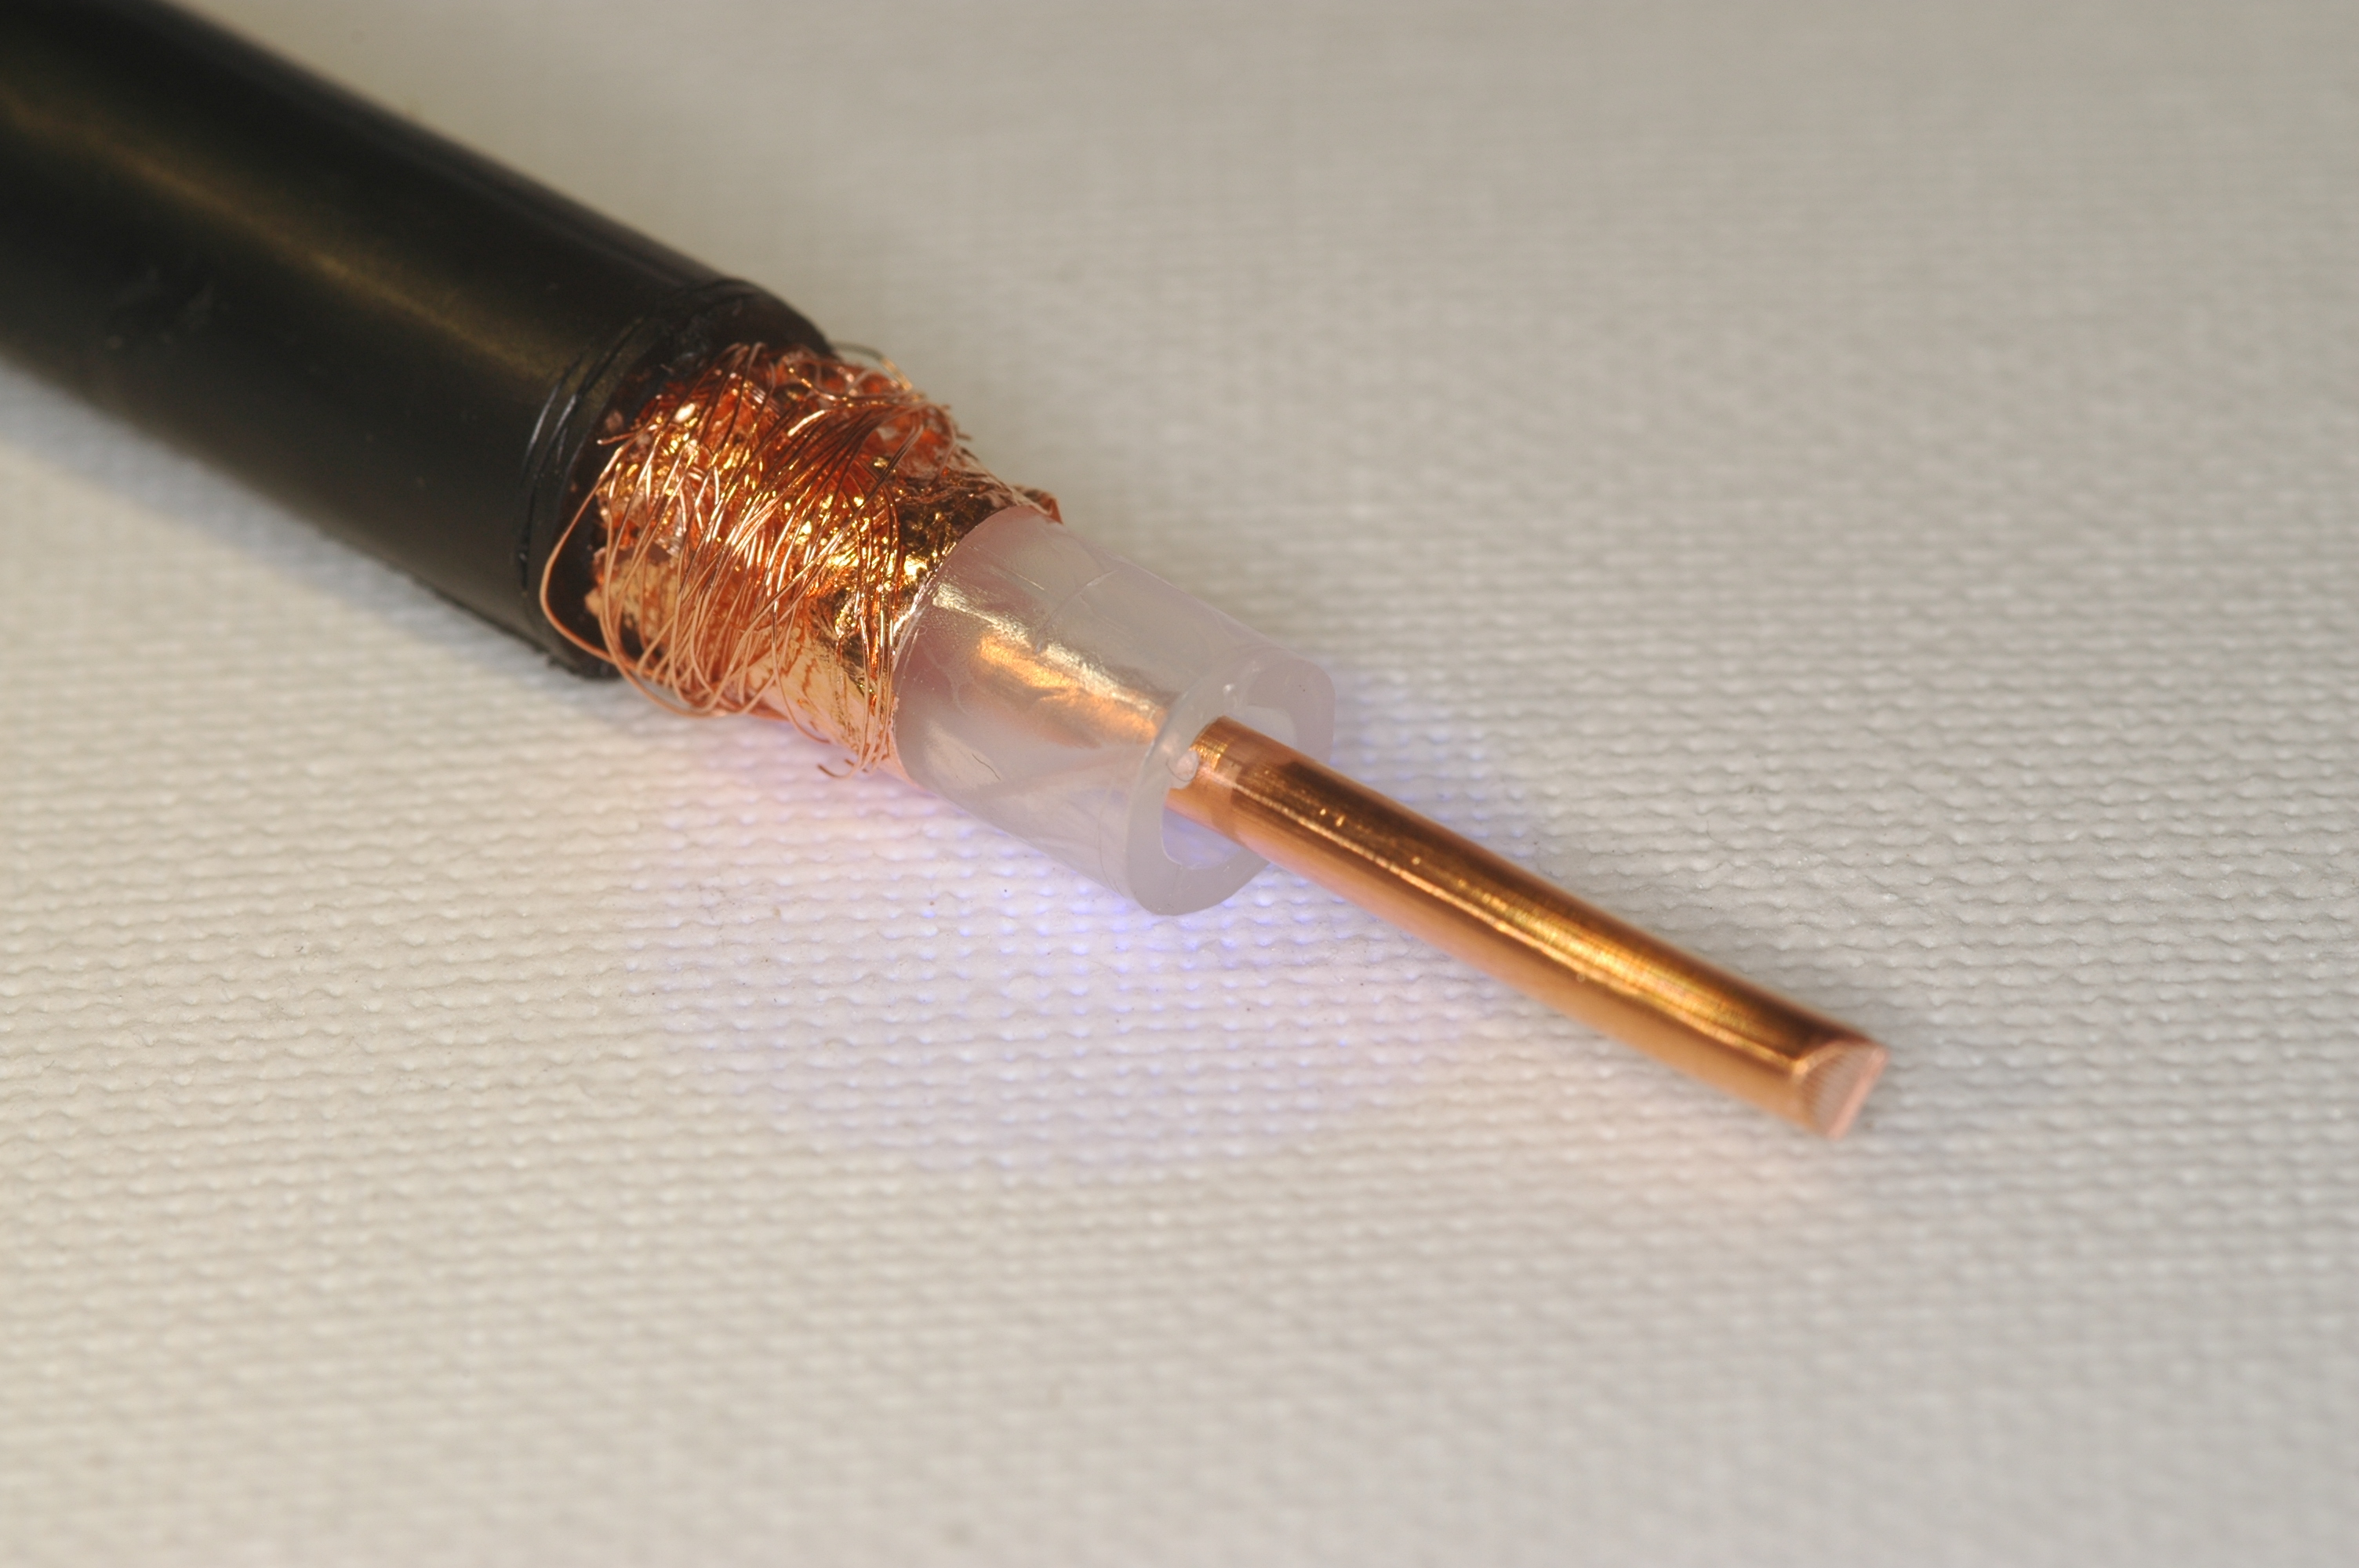
\includegraphics[width=0.85\textwidth]{foto/65}
    \caption{\scriptsize Koaxial-Kabel im Detail}
    \label{n_Koax_Detail}
\end{figure}

    \end{column}
   \begin{column}{0.48\textwidth}
       \begin{itemize}
  \item Am weitesten verbreitet
  \item Voneinander isolierter Innen- und Außenleiter
  \item Umgeben von Schutzmantel
  \item Unterschiedliche Ausführungen möglich
  \end{itemize}

   \end{column}
\end{columns}

\end{frame}

\begin{frame}
\frametitle{Unterschiedliche Koaxialkabel}

\begin{figure}
    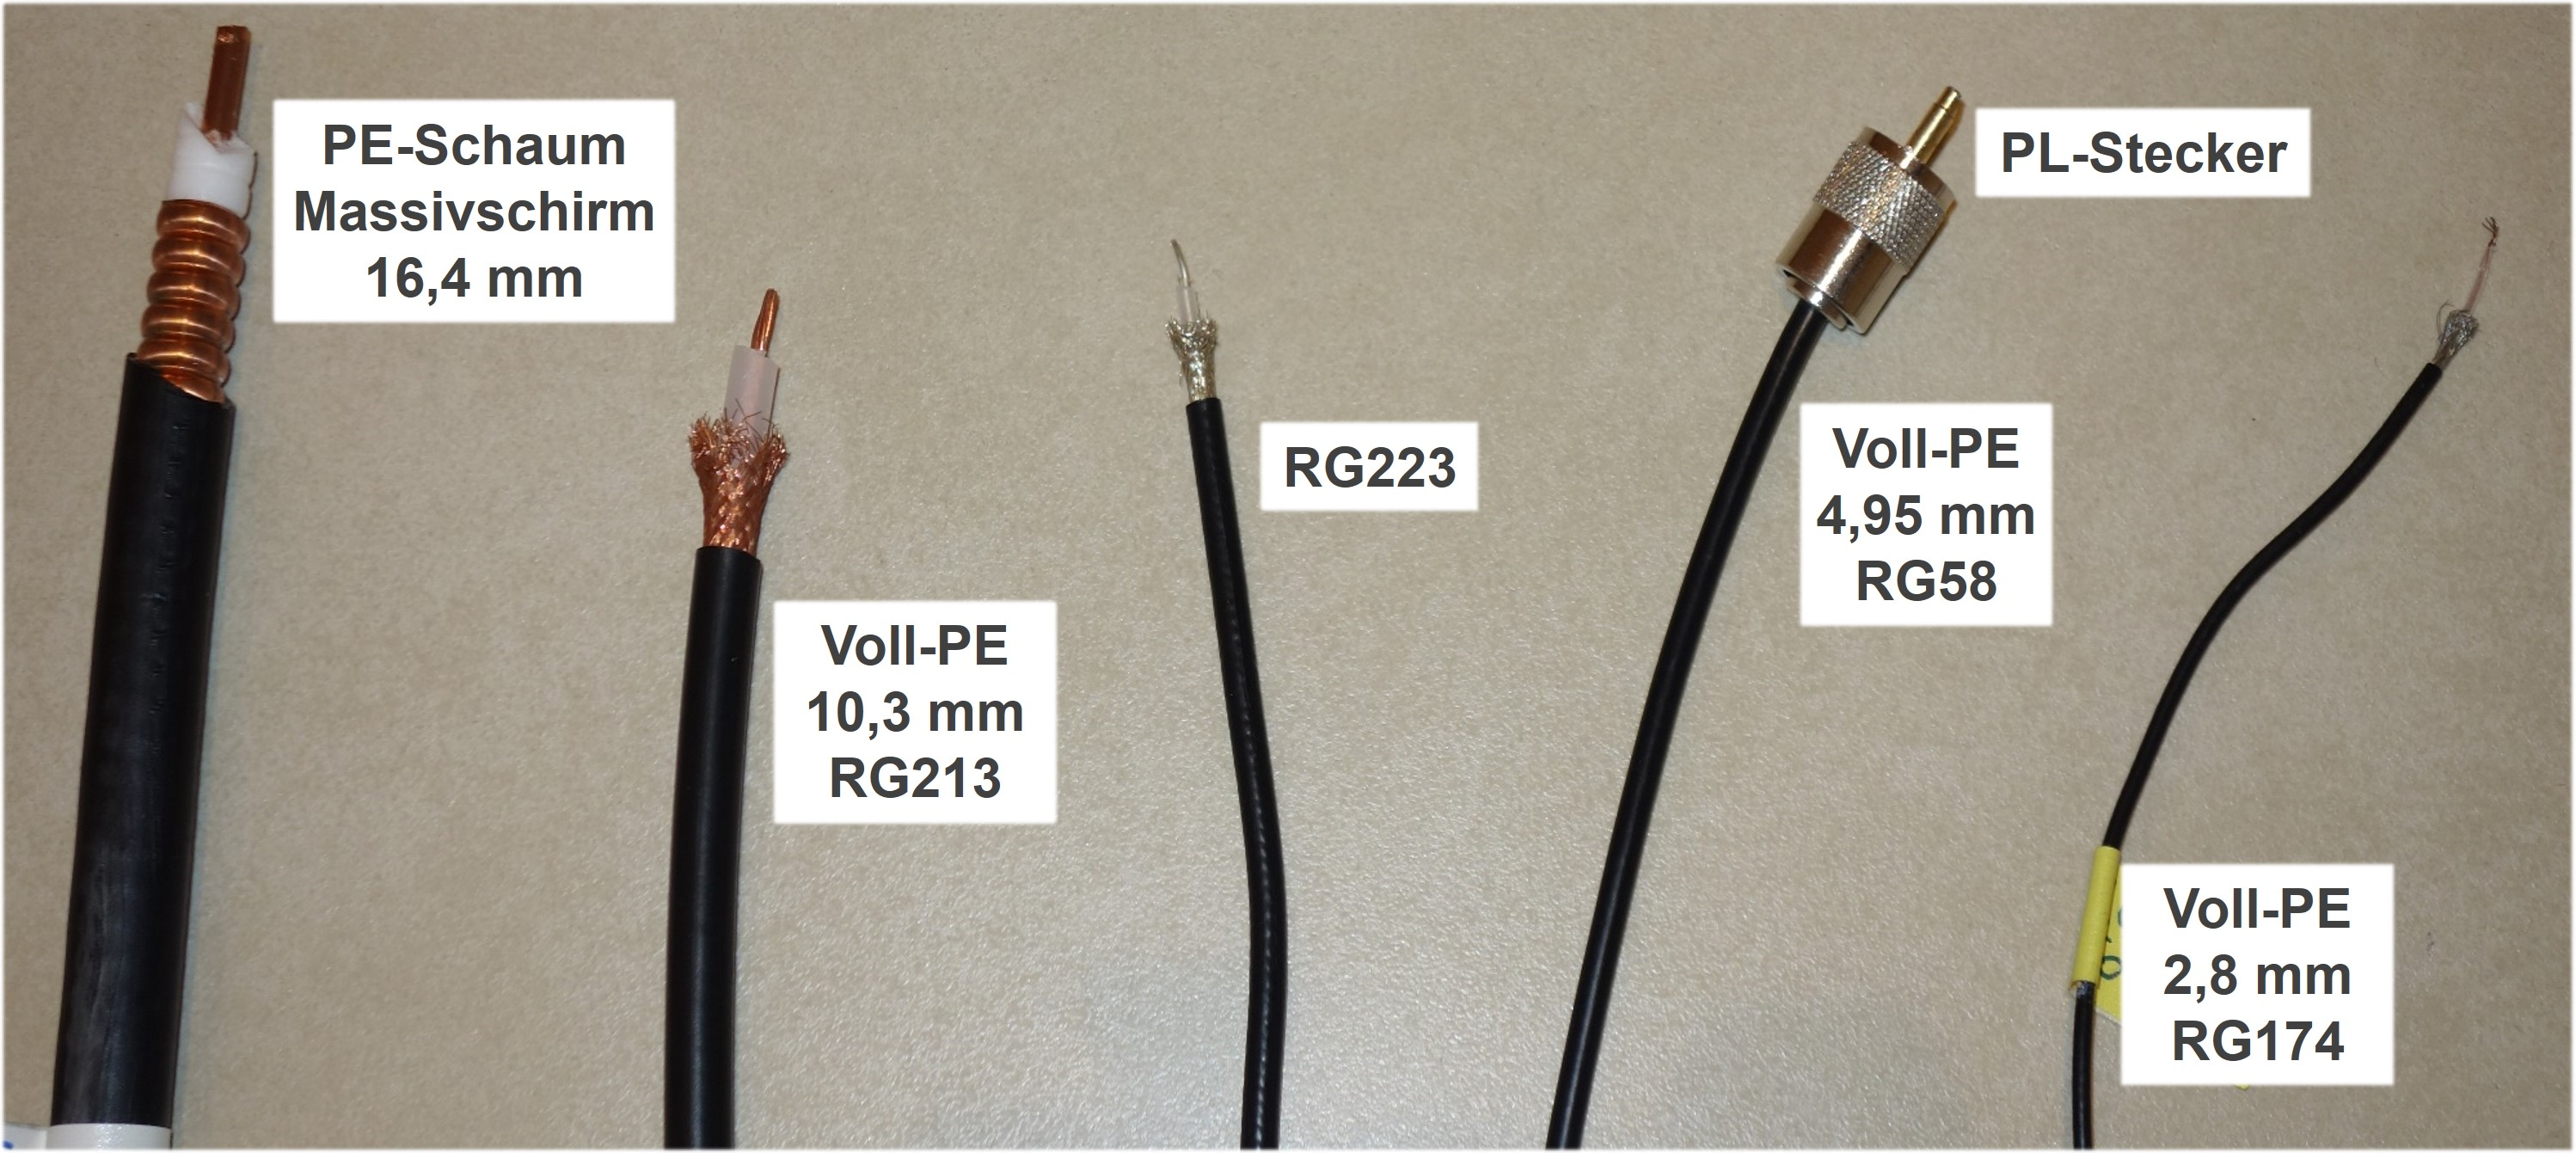
\includegraphics[width=0.85\textwidth]{foto/66}
    \caption{\scriptsize Beispiele gebräuchlicher Koaxialkabel}
    \label{n_Koaxialkabel}
\end{figure}
\end{frame}

\begin{frame}
\frametitle{Kabeldämpfung}
\begin{itemize}
  \item Im Koaxialkabel entsteht Verlust durch Umsetzung von Sendeleistung in Wärme
  \item Der Verlust wird \emph{Kabeldämpfung} genannt
  \item Messung in Dezibel (dB) je 100~m
  \item Verluste steigen mit zunehmender Länge und Frequenz
  \end{itemize}
\end{frame}

\begin{frame}
\only<1>{
\begin{QQuestion}{NG207}{Zwischen VHF/UHF-Transceiver und Antenne soll ein Koaxialkabel verwendet werden. Welche Aspekte sind neben dem richtigen Wellenwiderstand bei der Kabelauswahl zu beachten?}{Die Kabellänge hat keinen Einfluss auf die Kabeldämpfung.}
{Die Dämpfung sinkt mit zunehmender Länge und Frequenz.}
{Die Verluste steigen mit zunehmender Länge und Frequenz.}
{Die Frequenz hat keinen Einfluss auf die Kabeldämpfung.}
\end{QQuestion}

}
\only<2>{
\begin{QQuestion}{NG207}{Zwischen VHF/UHF-Transceiver und Antenne soll ein Koaxialkabel verwendet werden. Welche Aspekte sind neben dem richtigen Wellenwiderstand bei der Kabelauswahl zu beachten?}{Die Kabellänge hat keinen Einfluss auf die Kabeldämpfung.}
{Die Dämpfung sinkt mit zunehmender Länge und Frequenz.}
{\textbf{\textcolor{DARCgreen}{Die Verluste steigen mit zunehmender Länge und Frequenz.}}}
{Die Frequenz hat keinen Einfluss auf die Kabeldämpfung.}
\end{QQuestion}

}
\end{frame}

\begin{frame}
\frametitle{Wellenwiderstand}
\begin{columns}
    \begin{column}{0.48\textwidth}
    \begin{itemize}
  \item Wird in Ohm (Ω) angegeben
  \item Eigenschaft der Leitung, wie den Aufbau (z.B. Abstand zwischen Innen- und Außenleiter)
  \item Länge hat keine Auswirkung
  \end{itemize}

    \end{column}
   \begin{column}{0.48\textwidth}
       
    \pause
    \begin{itemize}
  \item Antennenanschluss von Amateurfunkgeräten: 50~Ω
  \item Koaxialkabel im Amateurfunk: 50~Ω
  \item Fernsehtechnik: 75~Ω
  \item Selten sind 60~Ω anzufinden
  \end{itemize}



   \end{column}
\end{columns}

\end{frame}

\begin{frame}
\only<1>{
\begin{QQuestion}{NG201}{Koaxialkabel weisen typischerweise Wellenwiderstände von~...}{\num{50}, \num{75} und \qty{240}{\ohm} auf.}
{\num{50}, \num{300} und \qty{600}{\ohm} auf.}
{\num{60}, \num{120} und \qty{240}{\ohm} auf.}
{\num{50}, \num{60} und \qty{75}{\ohm} auf.}
\end{QQuestion}

}
\only<2>{
\begin{QQuestion}{NG201}{Koaxialkabel weisen typischerweise Wellenwiderstände von~...}{\num{50}, \num{75} und \qty{240}{\ohm} auf.}
{\num{50}, \num{300} und \qty{600}{\ohm} auf.}
{\num{60}, \num{120} und \qty{240}{\ohm} auf.}
{\textbf{\textcolor{DARCgreen}{\num{50}, \num{60} und \qty{75}{\ohm} auf.}}}
\end{QQuestion}

}
\end{frame}%ENDCONTENT


\section{Koaxialsteckverbinder}
\label{section:koaxsteckverbinder}
\begin{frame}%STARTCONTENT

\begin{columns}
    \begin{column}{0.48\textwidth}
    \begin{itemize}
  \item Bestehen aus Innen- und Außenleiter
  \item Außengehäuse mit Außenleiter verbunden
  \item Innenleiter mit Kontaktstift oder Kontaktöffnung verbunden
  \item Verbindung durch Löten oder Crimpen
  \end{itemize}

    \end{column}
   \begin{column}{0.48\textwidth}
       \begin{itemize}
  \item \emph{Stecker}: Kontaktstift nach außen
  \item \emph{Kupplung}: Kontaktöffnung nach innen
  \item Sonderform \emph{Buchse}: In Gerät eingebaute Kupplung
  \end{itemize}

   \end{column}
\end{columns}

\end{frame}

\begin{frame}Häufige Koaxialsteckverbinder im Amateurfunk
\begin{columns}
    \begin{column}{0.48\textwidth}
    \begin{itemize}
  \item PL
  \item N
  \end{itemize}

    \end{column}
   \begin{column}{0.48\textwidth}
       \begin{itemize}
  \item BNC
  \item SMA
  \end{itemize}

   \end{column}
\end{columns}

\end{frame}

\begin{frame}
\frametitle{Hinweise zur Verwendung}
\begin{columns}
    \begin{column}{0.48\textwidth}
    \begin{itemize}
  \item Sorgsamer Umgang
  \item Fest verschrauben
  \item Innenleiter kann brechen
  \item Schirmung kann verrutschen
  \item Ggf. auf Kurzschluss prüfen
  \end{itemize}

    \end{column}
   \begin{column}{0.48\textwidth}
       \begin{itemize}
  \item Stecker passend zu Kabelstärke verwenden
  \item Stecker passend zu Kabeldurchmesser verwenden
  \end{itemize}

   \end{column}
\end{columns}

\end{frame}%ENDCONTENT


\section{PL-Steckverbinder}
\label{section:steckverbinder_pl}
\begin{frame}%STARTCONTENT
Einsatz: Kurzwelle bis zum \qty{2}{\metre}-Band
\begin{columns}
    \begin{column}{0.48\textwidth}
    
\begin{figure}
    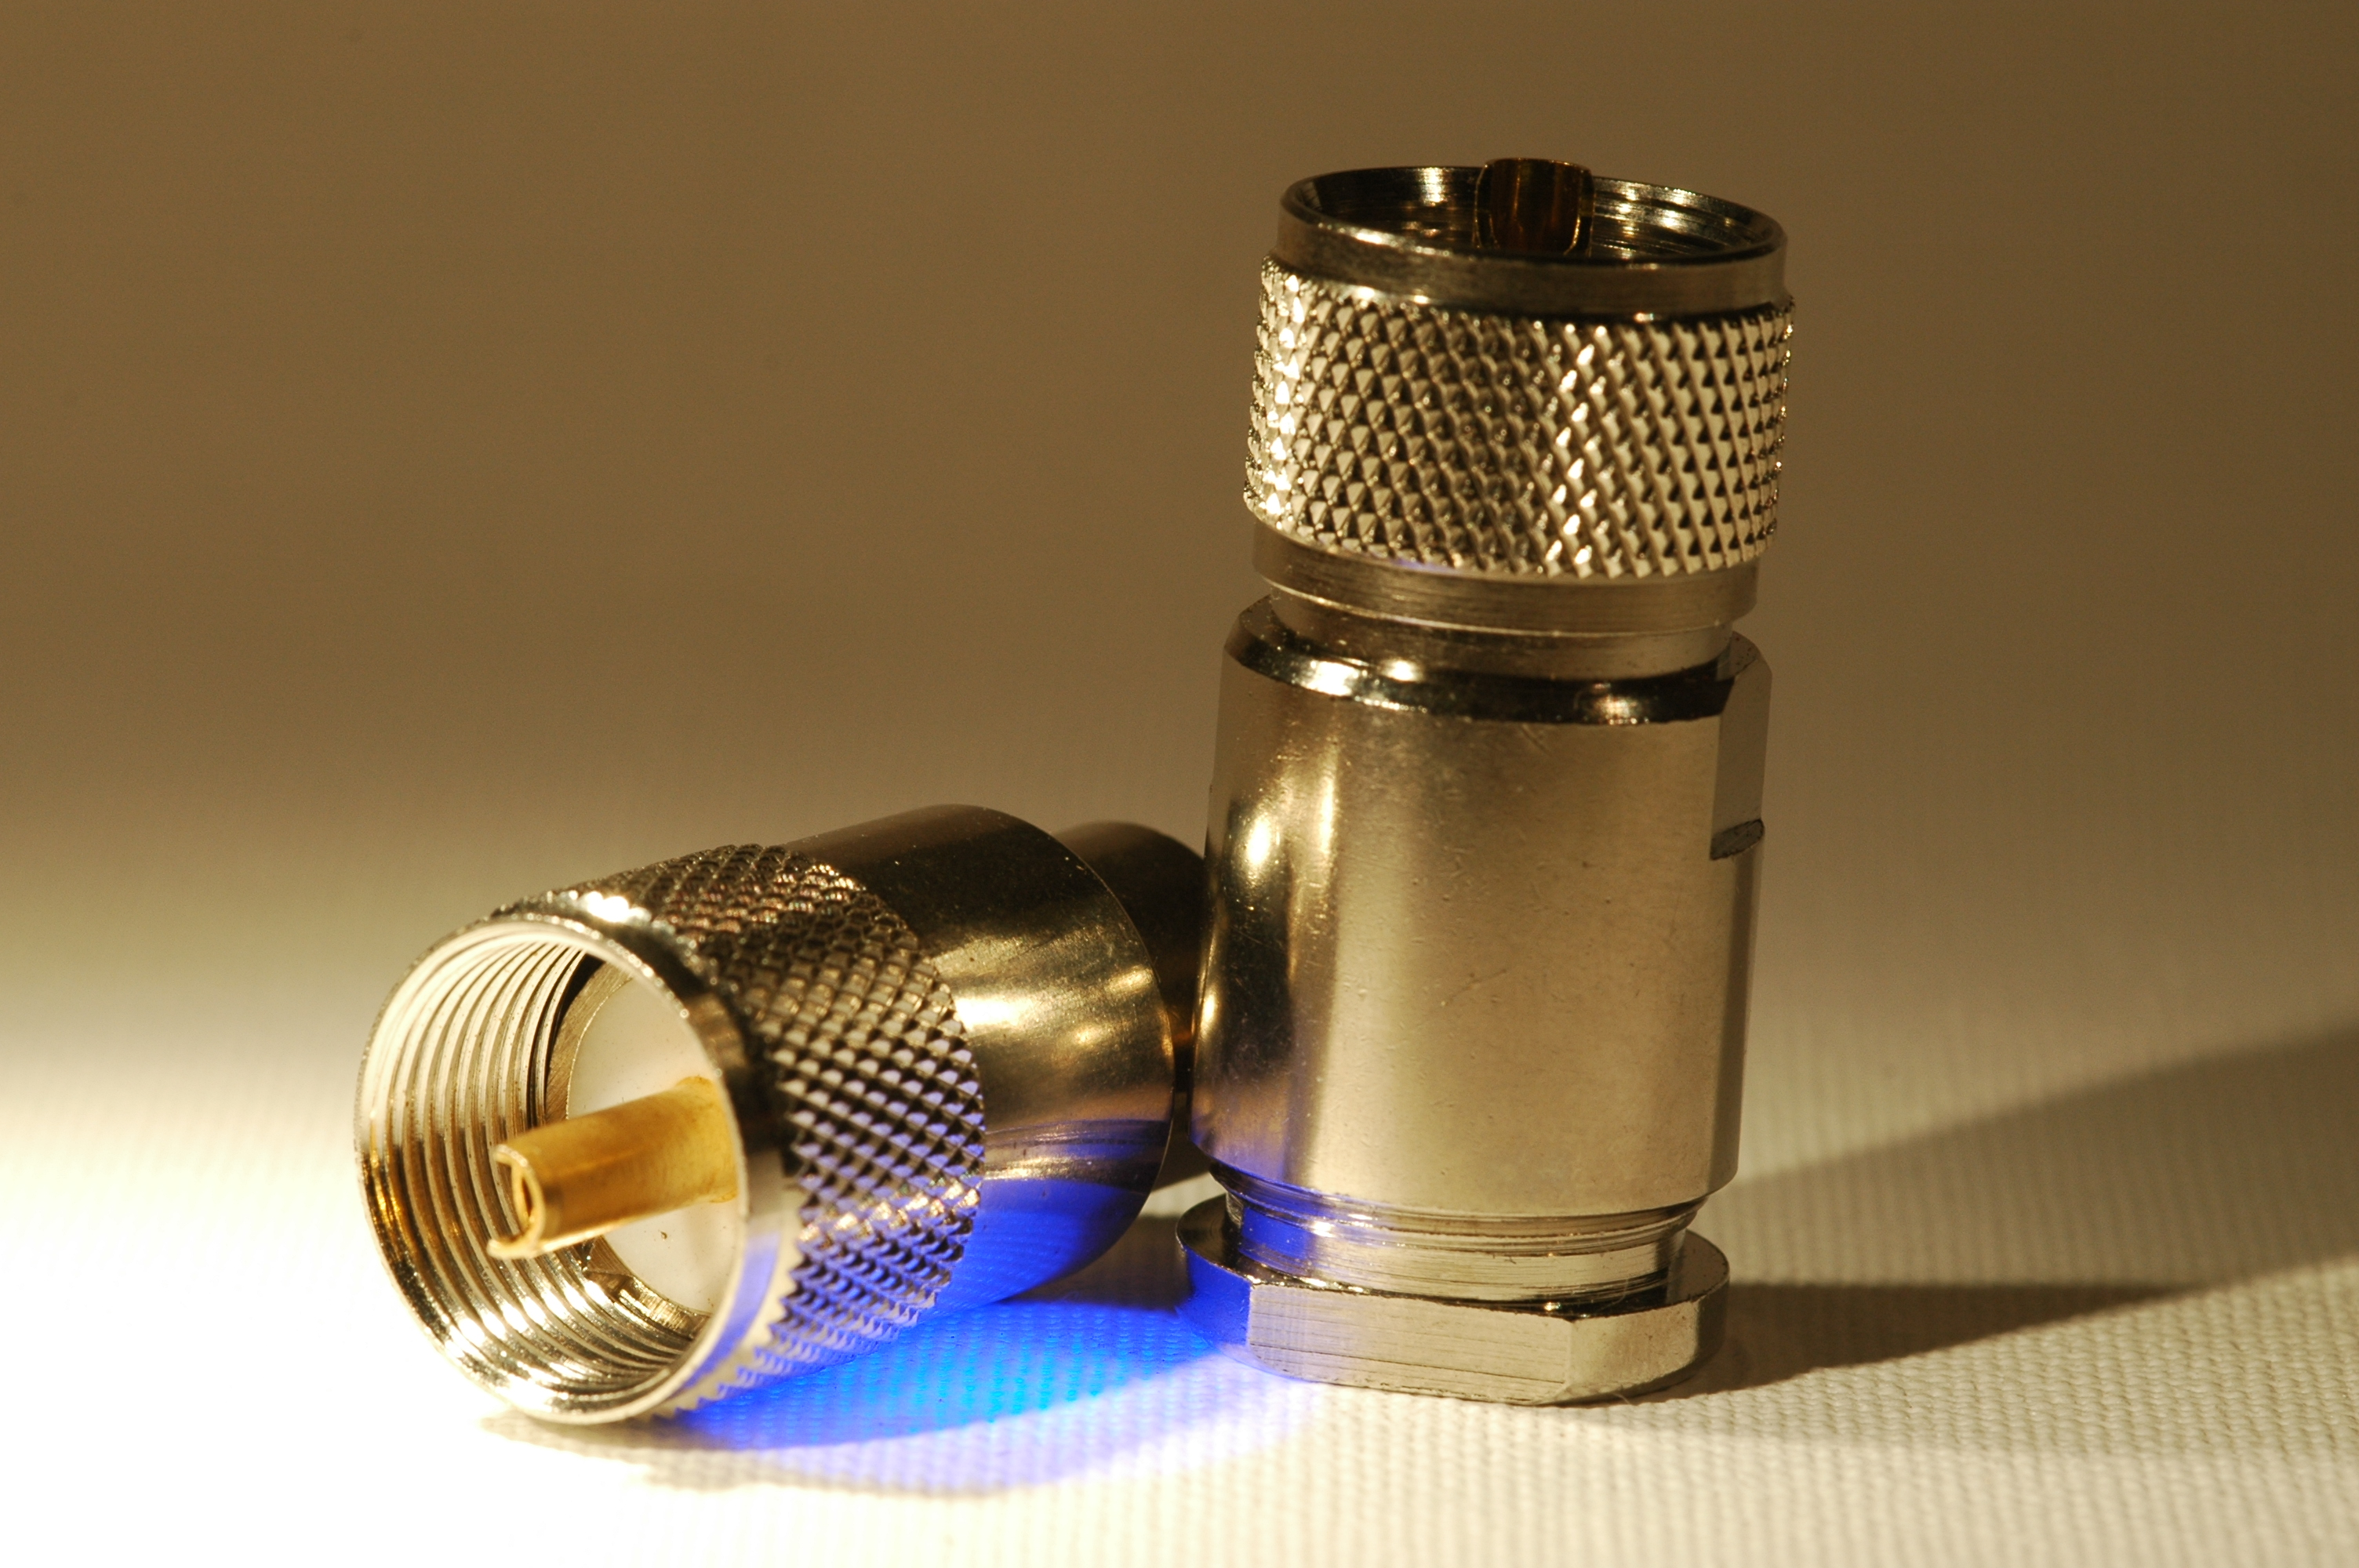
\includegraphics[width=0.85\textwidth]{foto/69}
    \caption{\scriptsize PL-Stecker}
    \label{n_koaxsteckverbinder_pl_stecker}
\end{figure}

    \end{column}
   \begin{column}{0.48\textwidth}
       
\begin{figure}
    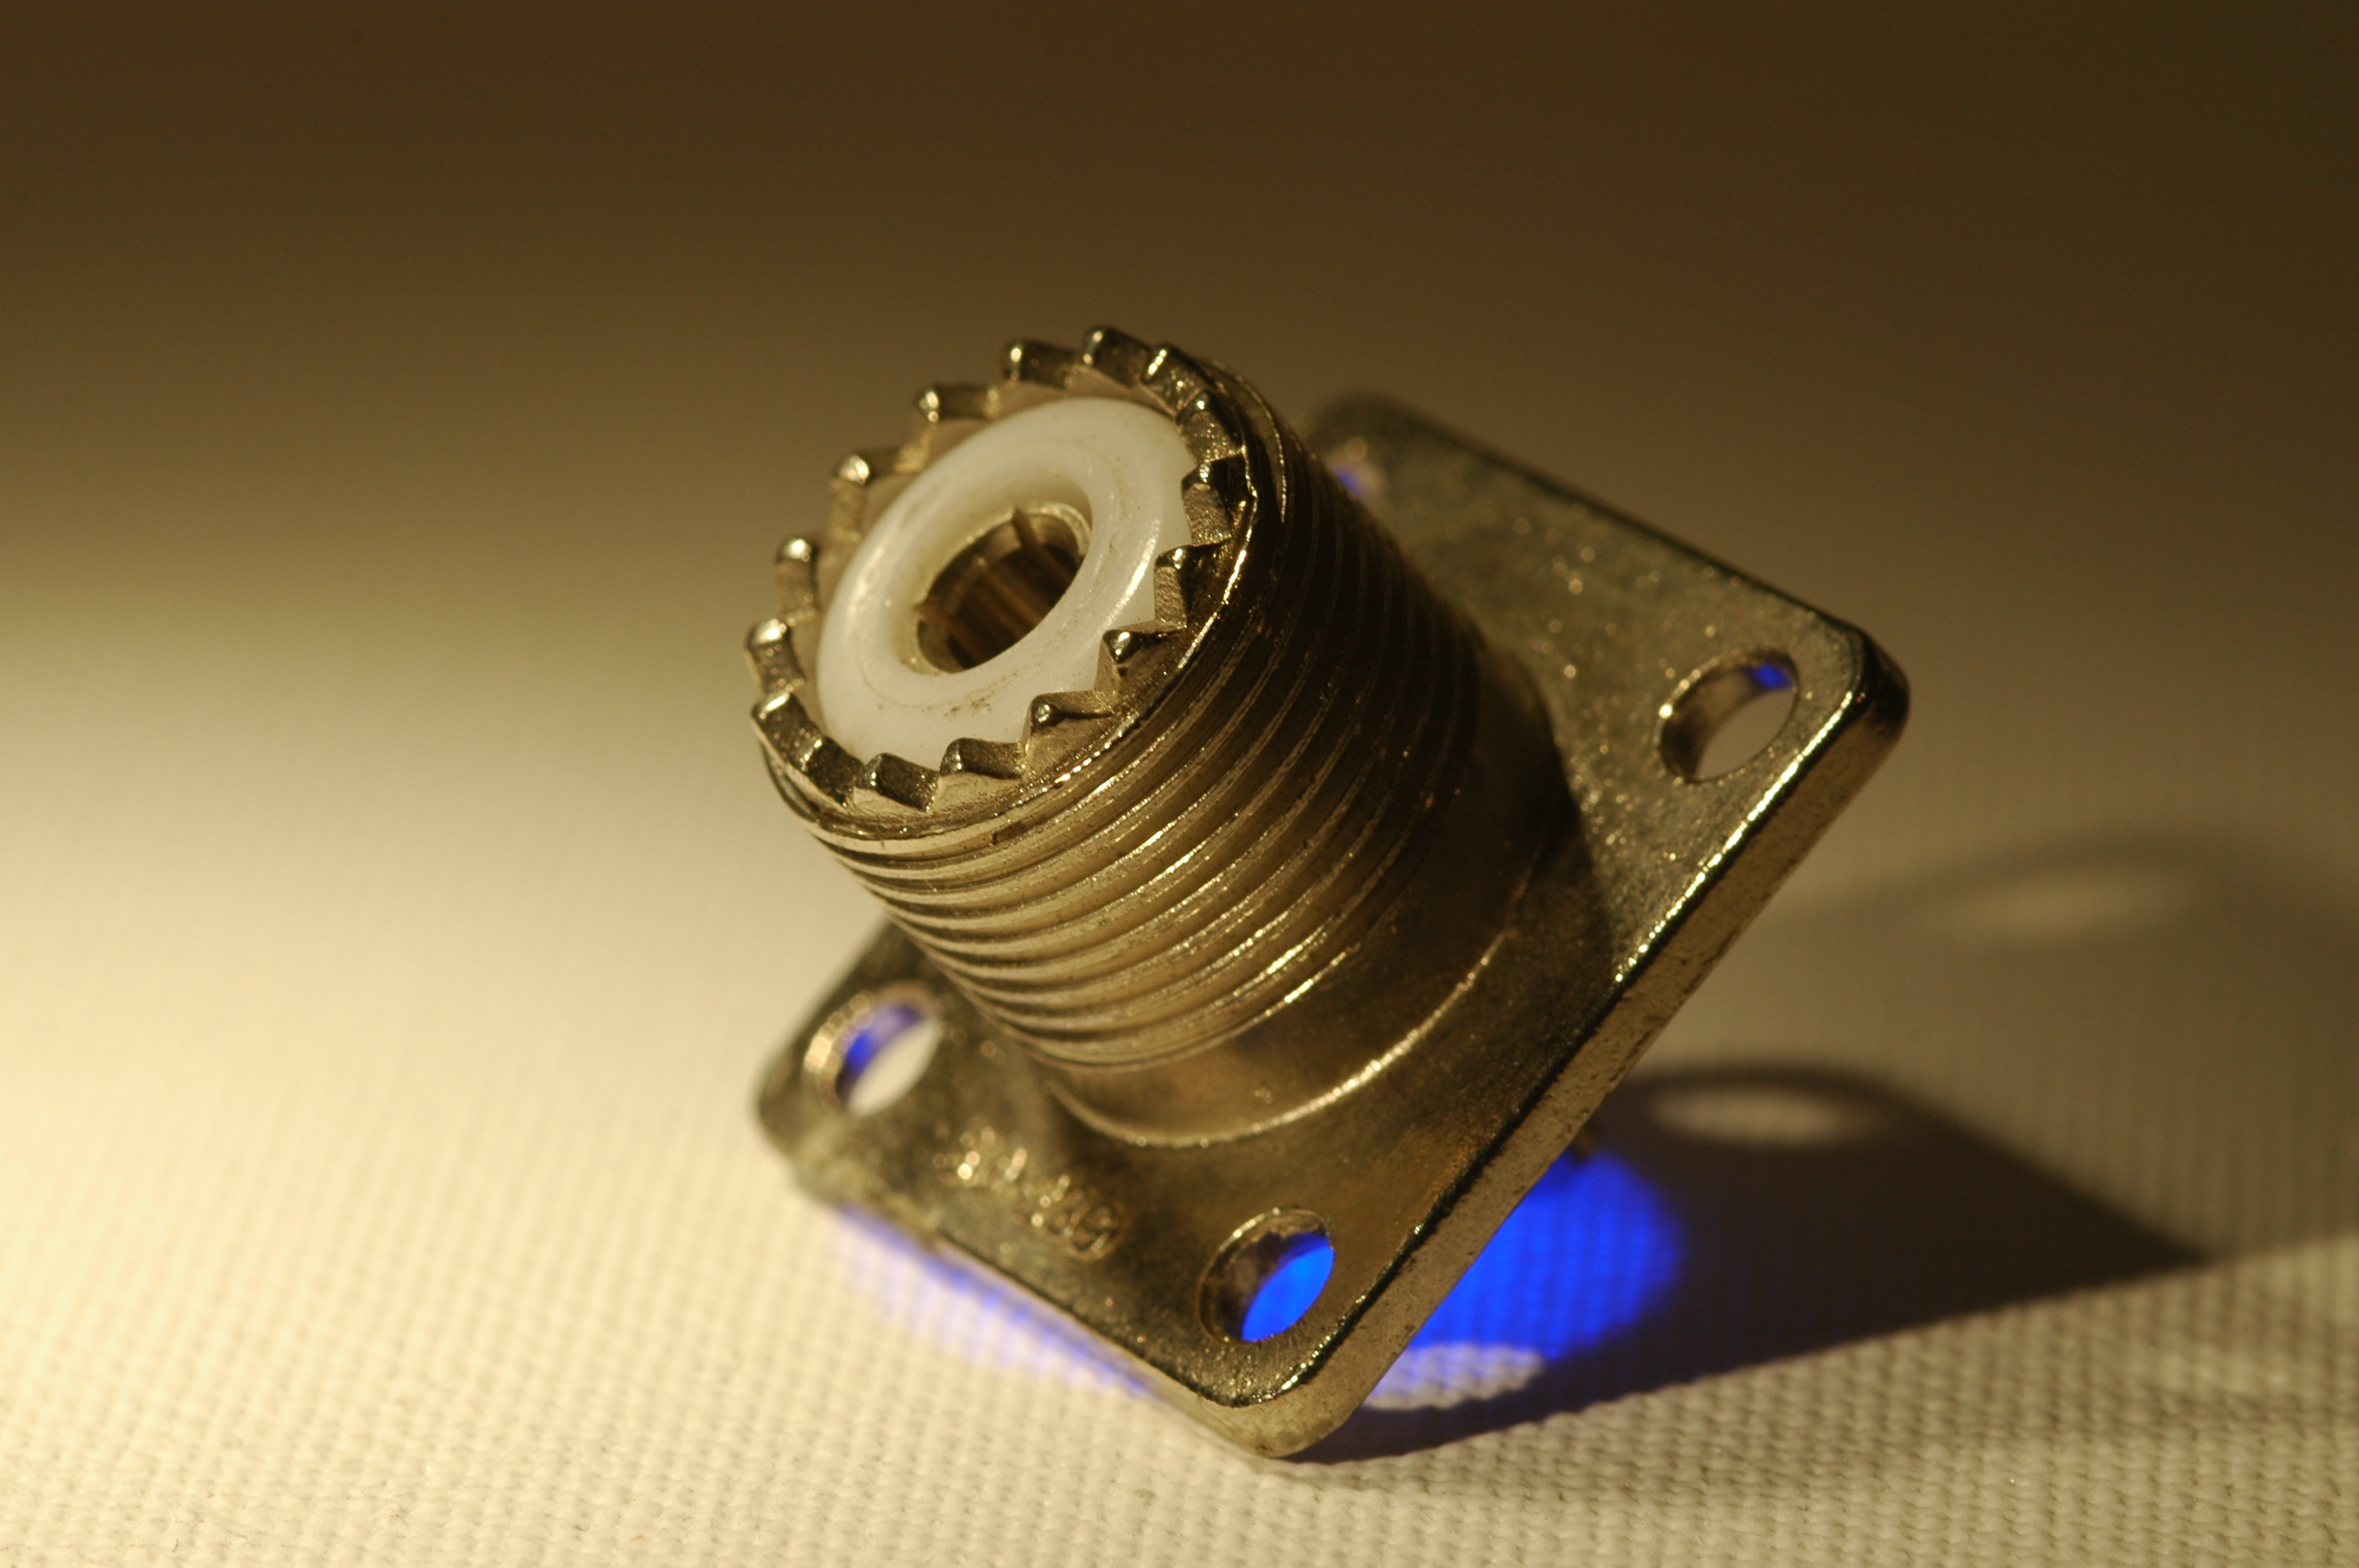
\includegraphics[width=0.85\textwidth]{foto/70}
    \caption{\scriptsize PL-Einbaubuchse}
    \label{n_koaxsteckverbinder_pl_einbaubuchse}
\end{figure}

   \end{column}
\end{columns}

\end{frame}

\begin{frame}
\only<1>{
\begin{PQuestion}{NG202}{Welches HF-Steckverbindungs-System wird in der folgenden Darstellung gezeigt?}{PL}
{BNC}
{SMA}
{N}
{\DARCimage{1.0\linewidth}{609include}}\end{PQuestion}

}
\only<2>{
\begin{PQuestion}{NG202}{Welches HF-Steckverbindungs-System wird in der folgenden Darstellung gezeigt?}{\textbf{\textcolor{DARCgreen}{PL}}}
{BNC}
{SMA}
{N}
{\DARCimage{1.0\linewidth}{609include}}\end{PQuestion}

}
\end{frame}%ENDCONTENT


\section{N-Steckverbinder}
\label{section:steckverbinder_n}
\begin{frame}%STARTCONTENT
Einsatz: \qty{2}{\metre}-Band bis in den GHz-Bereich
\begin{columns}
    \begin{column}{0.48\textwidth}
    
\begin{figure}
    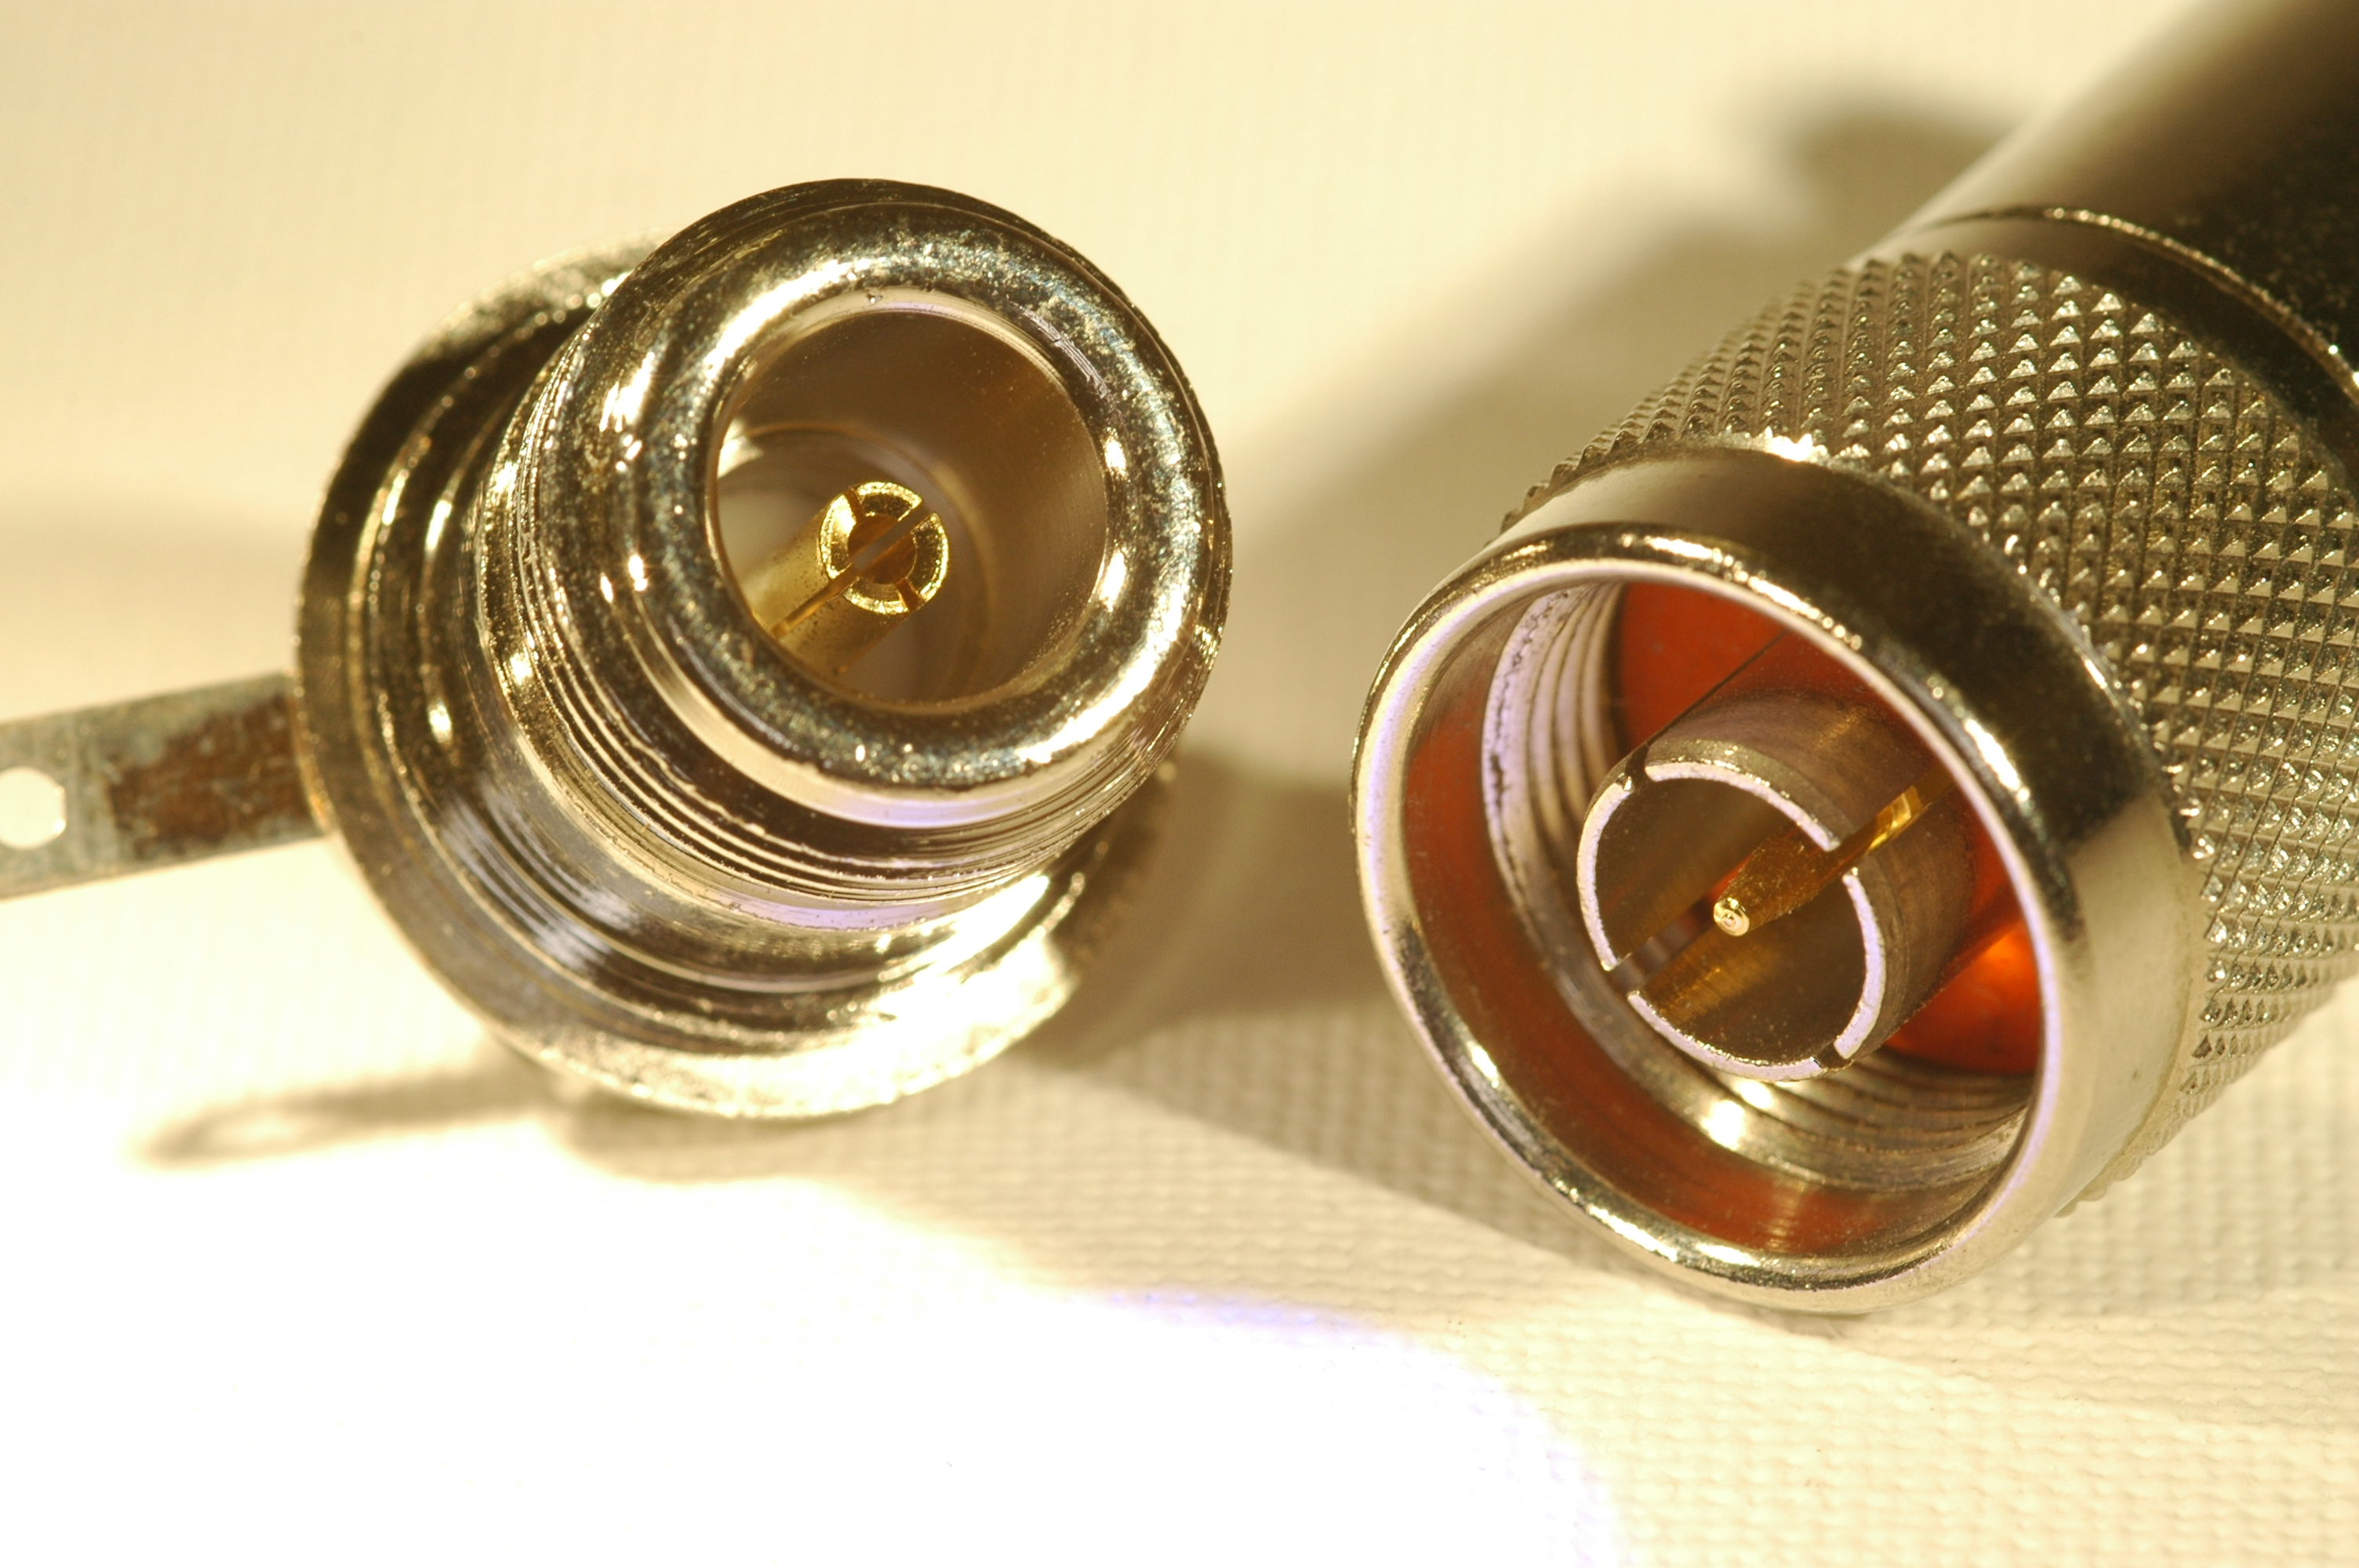
\includegraphics[width=0.85\textwidth]{foto/73}
    \caption{\scriptsize N-Einbaubuchse und N-Stecker}
    \label{n_koaxsteckverbinder_n_buchse_und_stecker}
\end{figure}

    \end{column}
   \begin{column}{0.48\textwidth}
       
\begin{figure}
    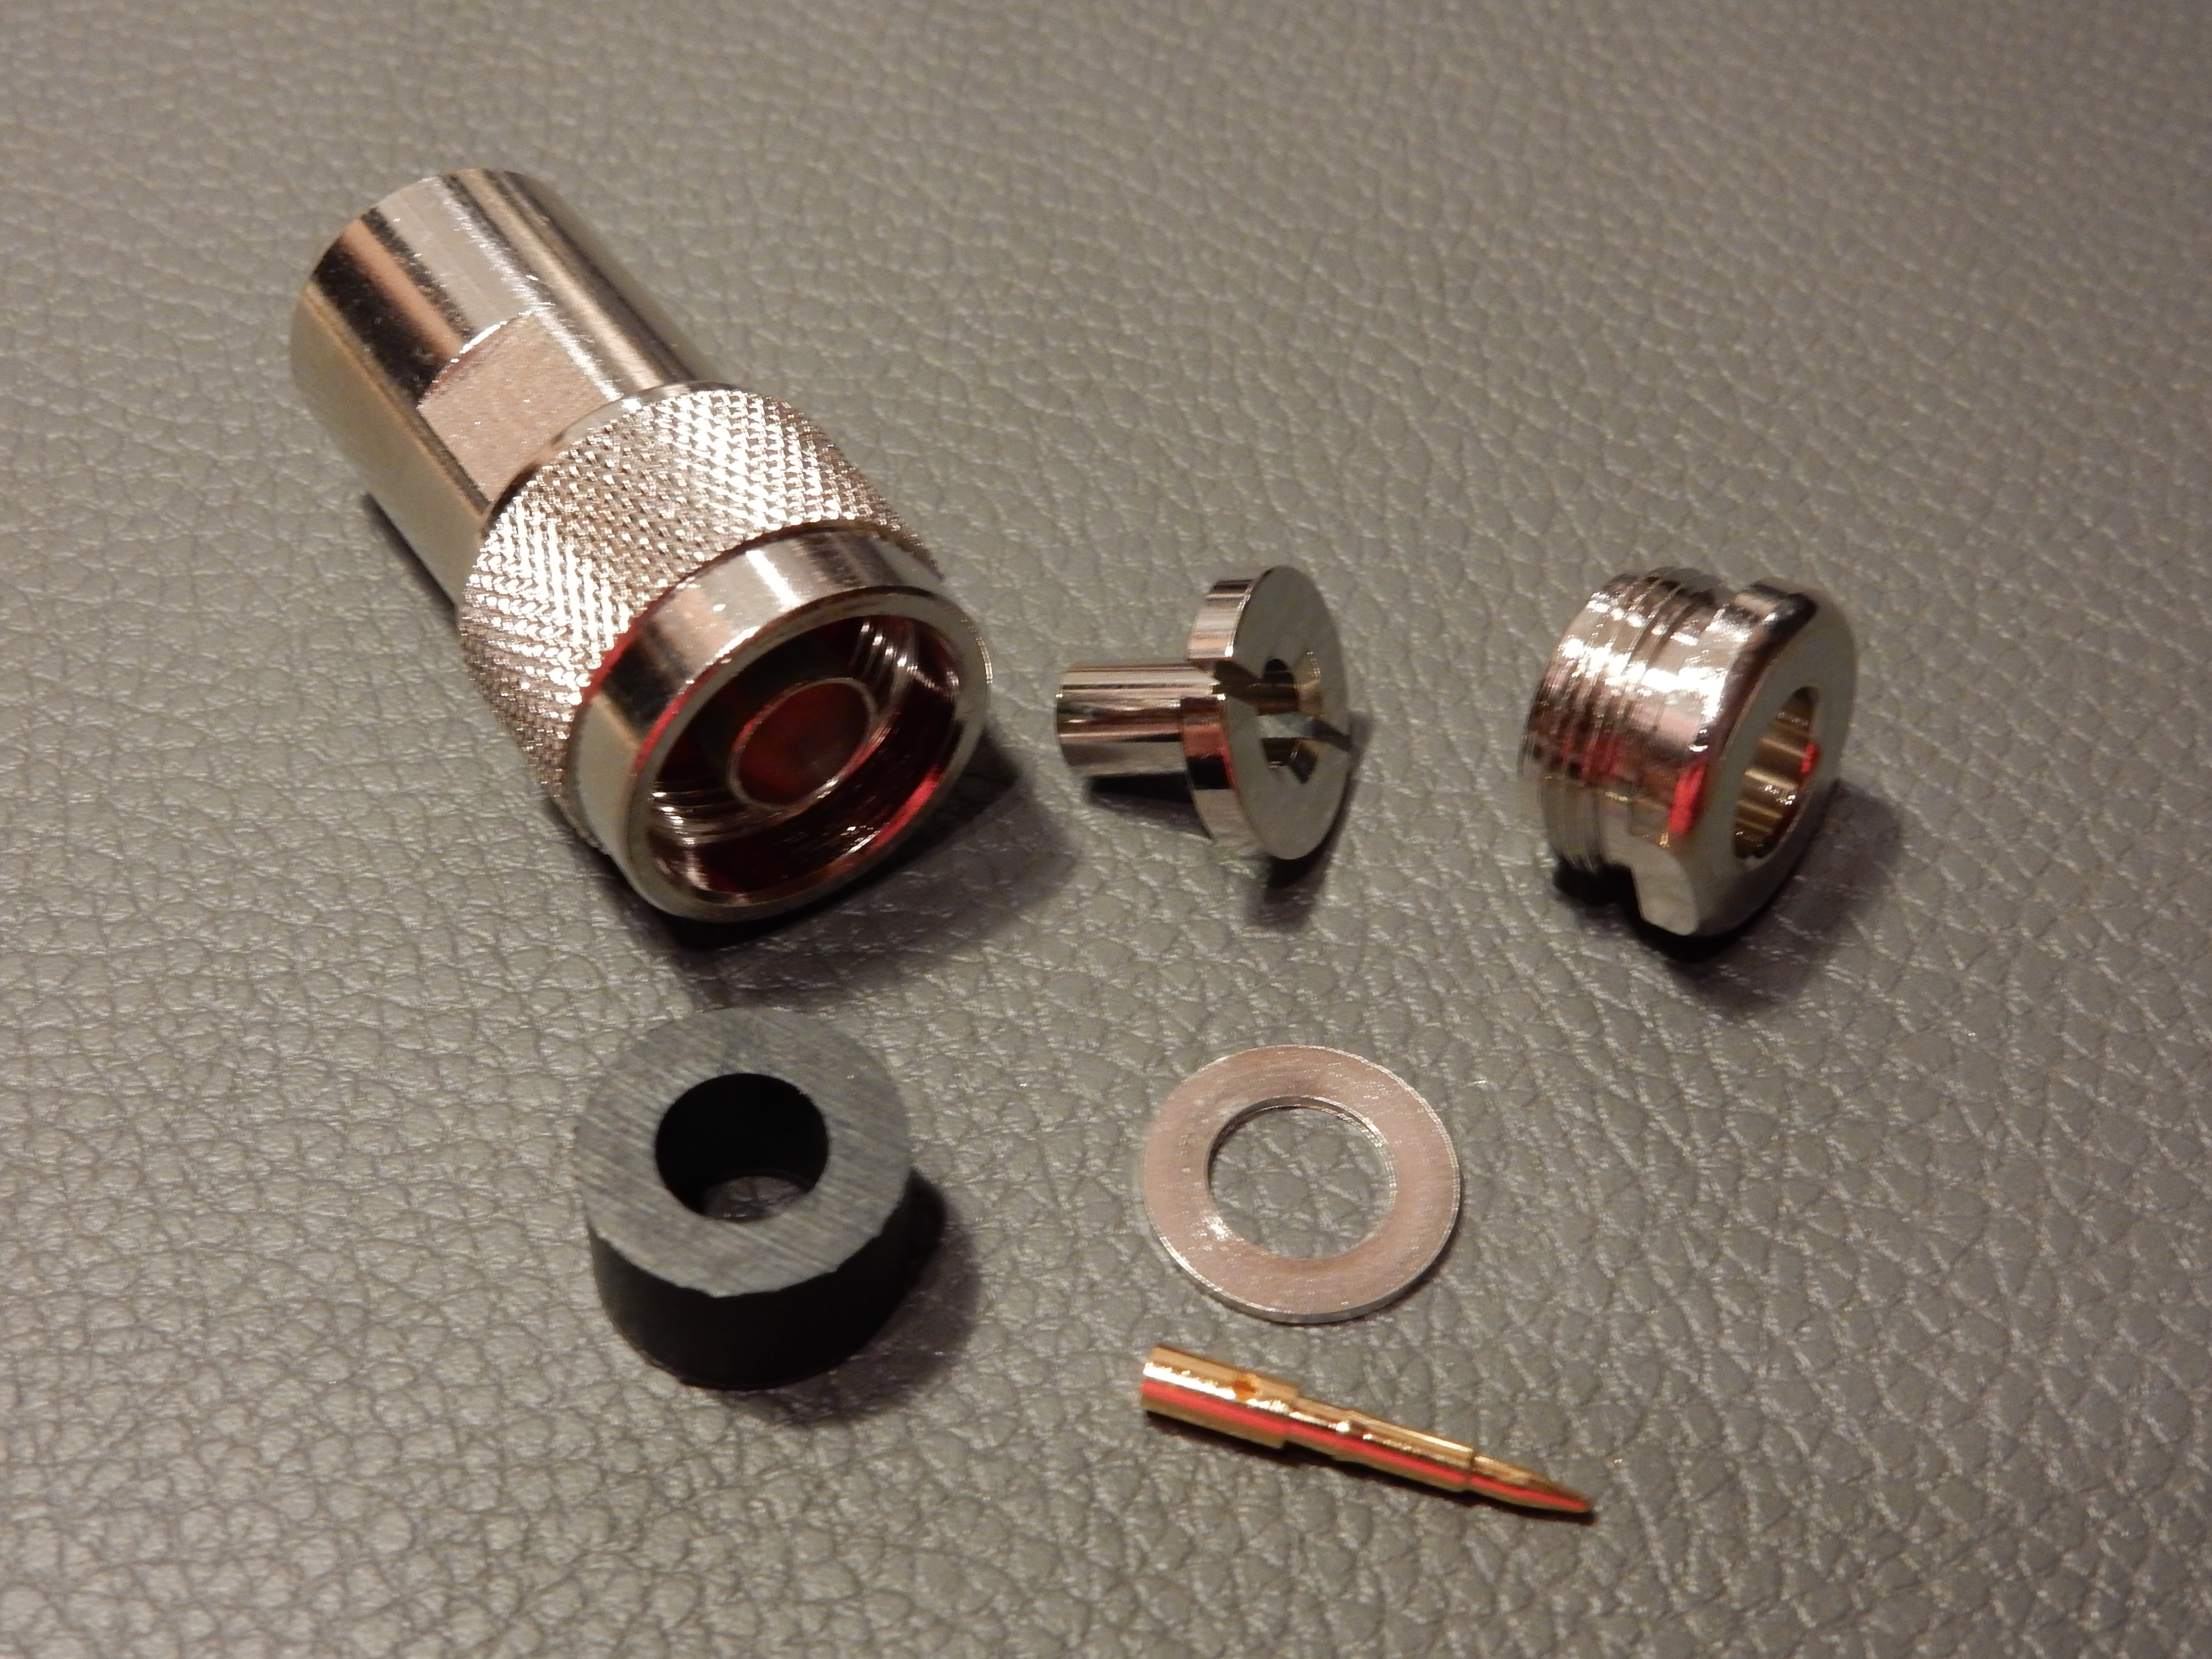
\includegraphics[width=0.85\textwidth]{foto/72}
    \caption{\scriptsize Ein N-Stecker vor seiner Montage}
    \label{n_koaxsteckverbinder_n_stecker}
\end{figure}

   \end{column}
\end{columns}

\end{frame}

\begin{frame}
\only<1>{
\begin{PQuestion}{NG204}{Welches HF-Steckverbindungs-System wird in der folgenden Darstellung gezeigt? }{SMA}
{PL}
{N}
{BNC}
{\DARCimage{1.0\linewidth}{610include}}\end{PQuestion}

}
\only<2>{
\begin{PQuestion}{NG204}{Welches HF-Steckverbindungs-System wird in der folgenden Darstellung gezeigt? }{SMA}
{PL}
{\textbf{\textcolor{DARCgreen}{N}}}
{BNC}
{\DARCimage{1.0\linewidth}{610include}}\end{PQuestion}

}
\end{frame}%ENDCONTENT


\section{BNC-Steckverbinder}
\label{section:steckverbinder_bnc}
\begin{frame}%STARTCONTENT
Einsatz: Für Funkgeräte mit kleiner Leistung bis hinauf zum \qty{70}{\centi\metre}-Band und in der Messtechnik


\begin{figure}
    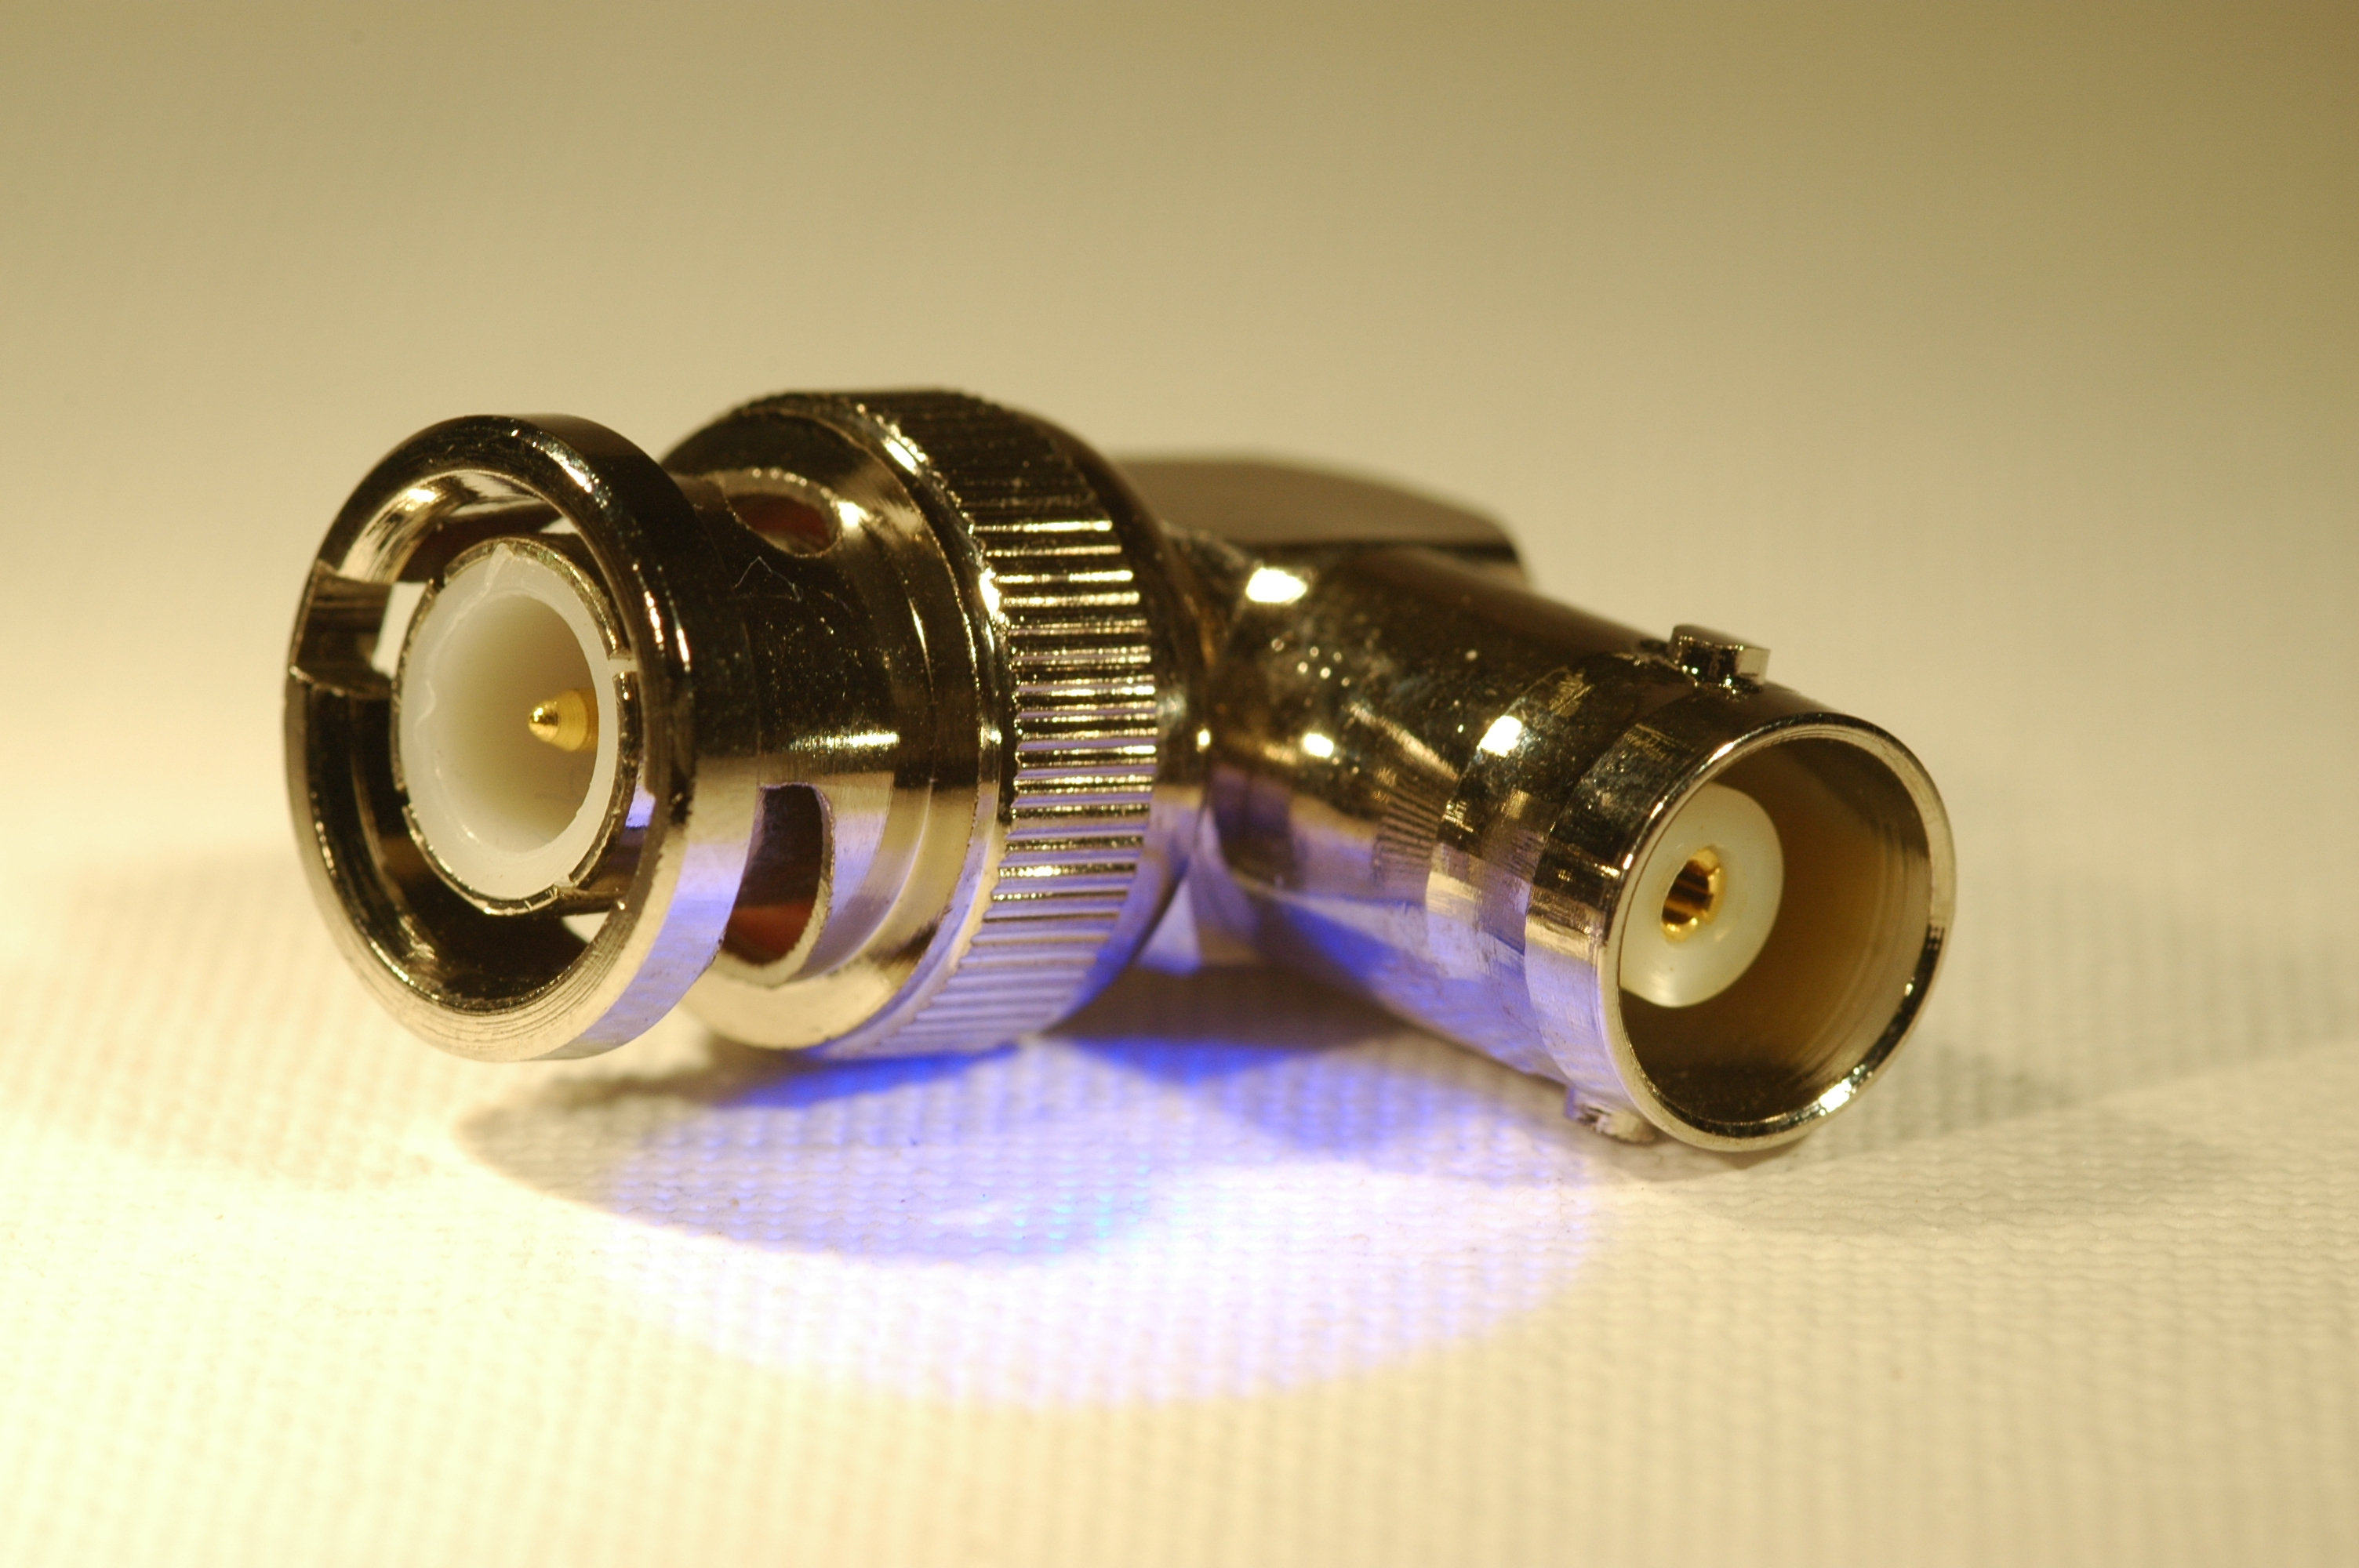
\includegraphics[width=0.85\textwidth]{foto/71}
    \caption{\scriptsize BNC-Winkeladapter mit Stecker links und Kupplung rechts}
    \label{n_koaxsteckverbinder_bnc}
\end{figure}

\end{frame}

\begin{frame}
\only<1>{
\begin{PQuestion}{NG203}{Welches HF-Steckverbindungs-System wird in der folgenden Darstellung gezeigt? }{N}
{SMA}
{PL}
{BNC}
{\DARCimage{1.0\linewidth}{608include}}\end{PQuestion}

}
\only<2>{
\begin{PQuestion}{NG203}{Welches HF-Steckverbindungs-System wird in der folgenden Darstellung gezeigt? }{N}
{SMA}
{PL}
{\textbf{\textcolor{DARCgreen}{BNC}}}
{\DARCimage{1.0\linewidth}{608include}}\end{PQuestion}

}
\end{frame}%ENDCONTENT


\section{SMA-Steckverbinder}
\label{section:steckverbinder_sma}
\begin{frame}%STARTCONTENT
Einsatz: Dort, wo man wenig Platz hat, auch bei hohen Frequenzen


\begin{figure}
    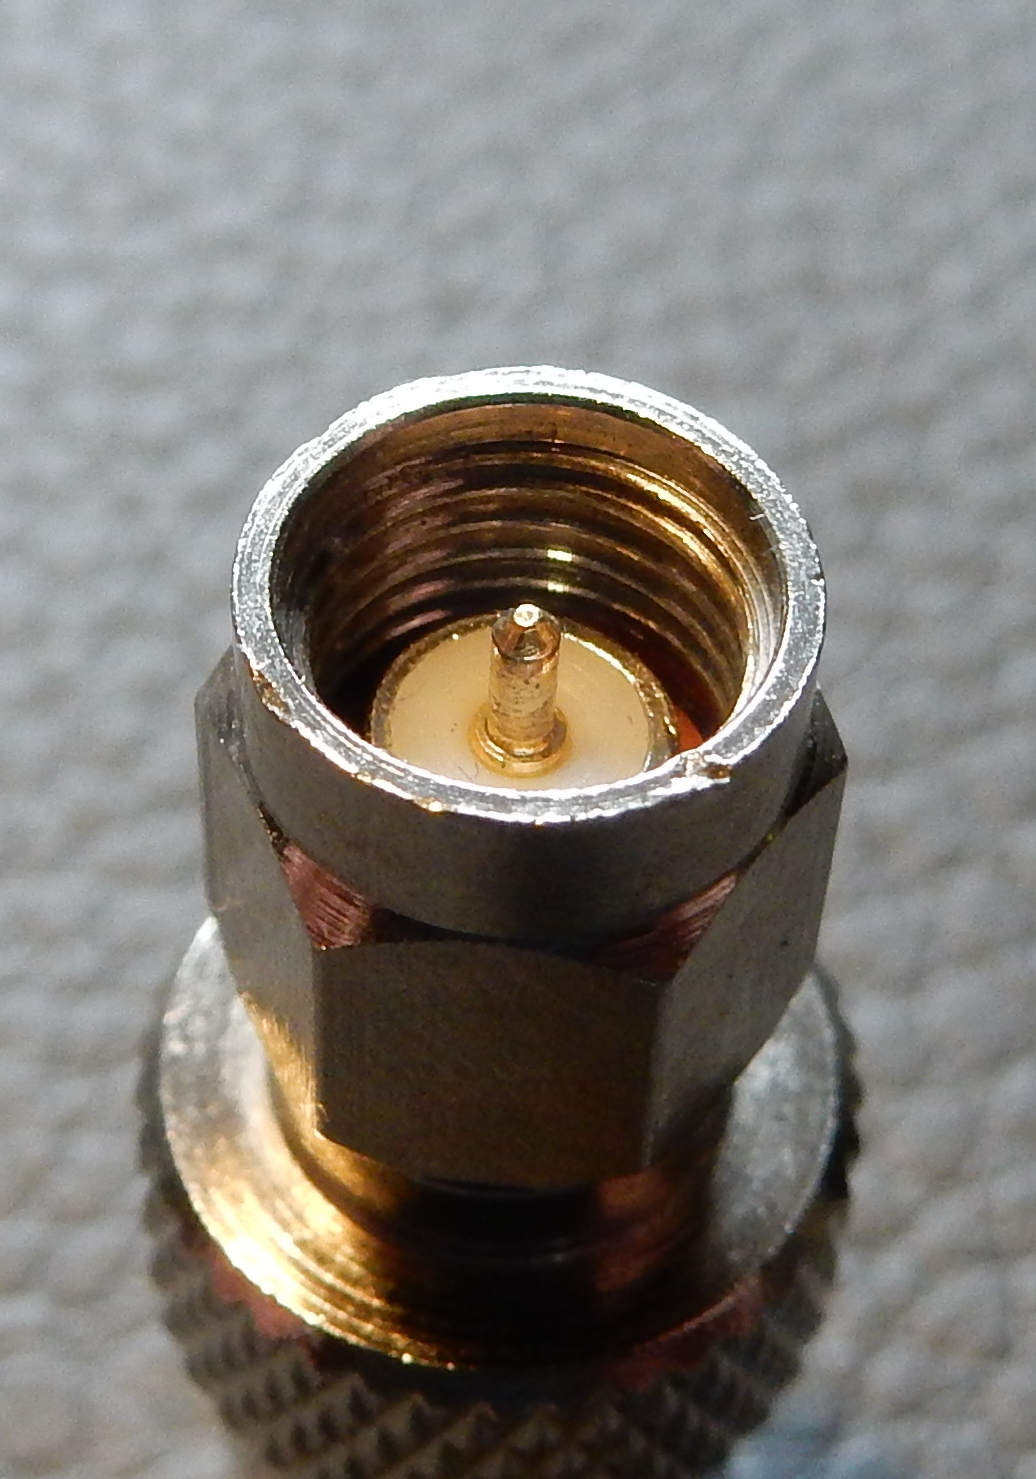
\includegraphics[width=0.85\textwidth]{foto/74}
    \caption{\scriptsize SMA-Stecker, hier stark vergrößert}
    \label{n_koaxsteckverbinder_sma}
\end{figure}

\end{frame}

\begin{frame}
\only<1>{
\begin{PQuestion}{NG205}{Welches HF-Steckverbindungs-System wird in der folgenden Darstellung gezeigt? }{PL}
{SMA}
{N}
{BNC}
{\DARCimage{1.0\linewidth}{611include}}\end{PQuestion}

}
\only<2>{
\begin{PQuestion}{NG205}{Welches HF-Steckverbindungs-System wird in der folgenden Darstellung gezeigt? }{PL}
{\textbf{\textcolor{DARCgreen}{SMA}}}
{N}
{BNC}
{\DARCimage{1.0\linewidth}{611include}}\end{PQuestion}

}
\end{frame}

\begin{frame}
\only<1>{
\begin{QQuestion}{NG206}{Welche der folgenden HF-Steckverbindungs-Systeme sind für hohe Frequenzen (oberhalb \qty{300}{\MHz}) am besten geeignet?}{BNC und Cinch}
{UHF und BNetzA}
{N und SMA}
{Cinch und SMA}
\end{QQuestion}

}
\only<2>{
\begin{QQuestion}{NG206}{Welche der folgenden HF-Steckverbindungs-Systeme sind für hohe Frequenzen (oberhalb \qty{300}{\MHz}) am besten geeignet?}{BNC und Cinch}
{UHF und BNetzA}
{\textbf{\textcolor{DARCgreen}{N und SMA}}}
{Cinch und SMA}
\end{QQuestion}

}
\end{frame}%ENDCONTENT


\section{Stehwellenverhältnis (SWR)}
\label{section:swr}
\begin{frame}%STARTCONTENT
\begin{itemize}
  \item Passt der Speisewiderstand der Antenne nicht zum Wellenwiderstand der Zuleitung, kommt es zu einer \emph{Reflexion}
  \item Sendeleistung wird zum Funkgerät zurück reflektiert $\rightarrow$ kann nicht an der Antenne abgestrahlt werden
  \item Stimmen Speisewiderstand der Antenne und Wellenwiderstand der Speiseleitung überein, liegt \emph{Anpassung} vor
  \end{itemize}
\end{frame}

\begin{frame}
\frametitle{SWR-Meter}
Misst gleichzeitig die Sendeleistung zur Antenne und die reflektierte, rücklaufende Leistung
\begin{columns}
    \begin{column}{0.48\textwidth}
    
\begin{figure}
    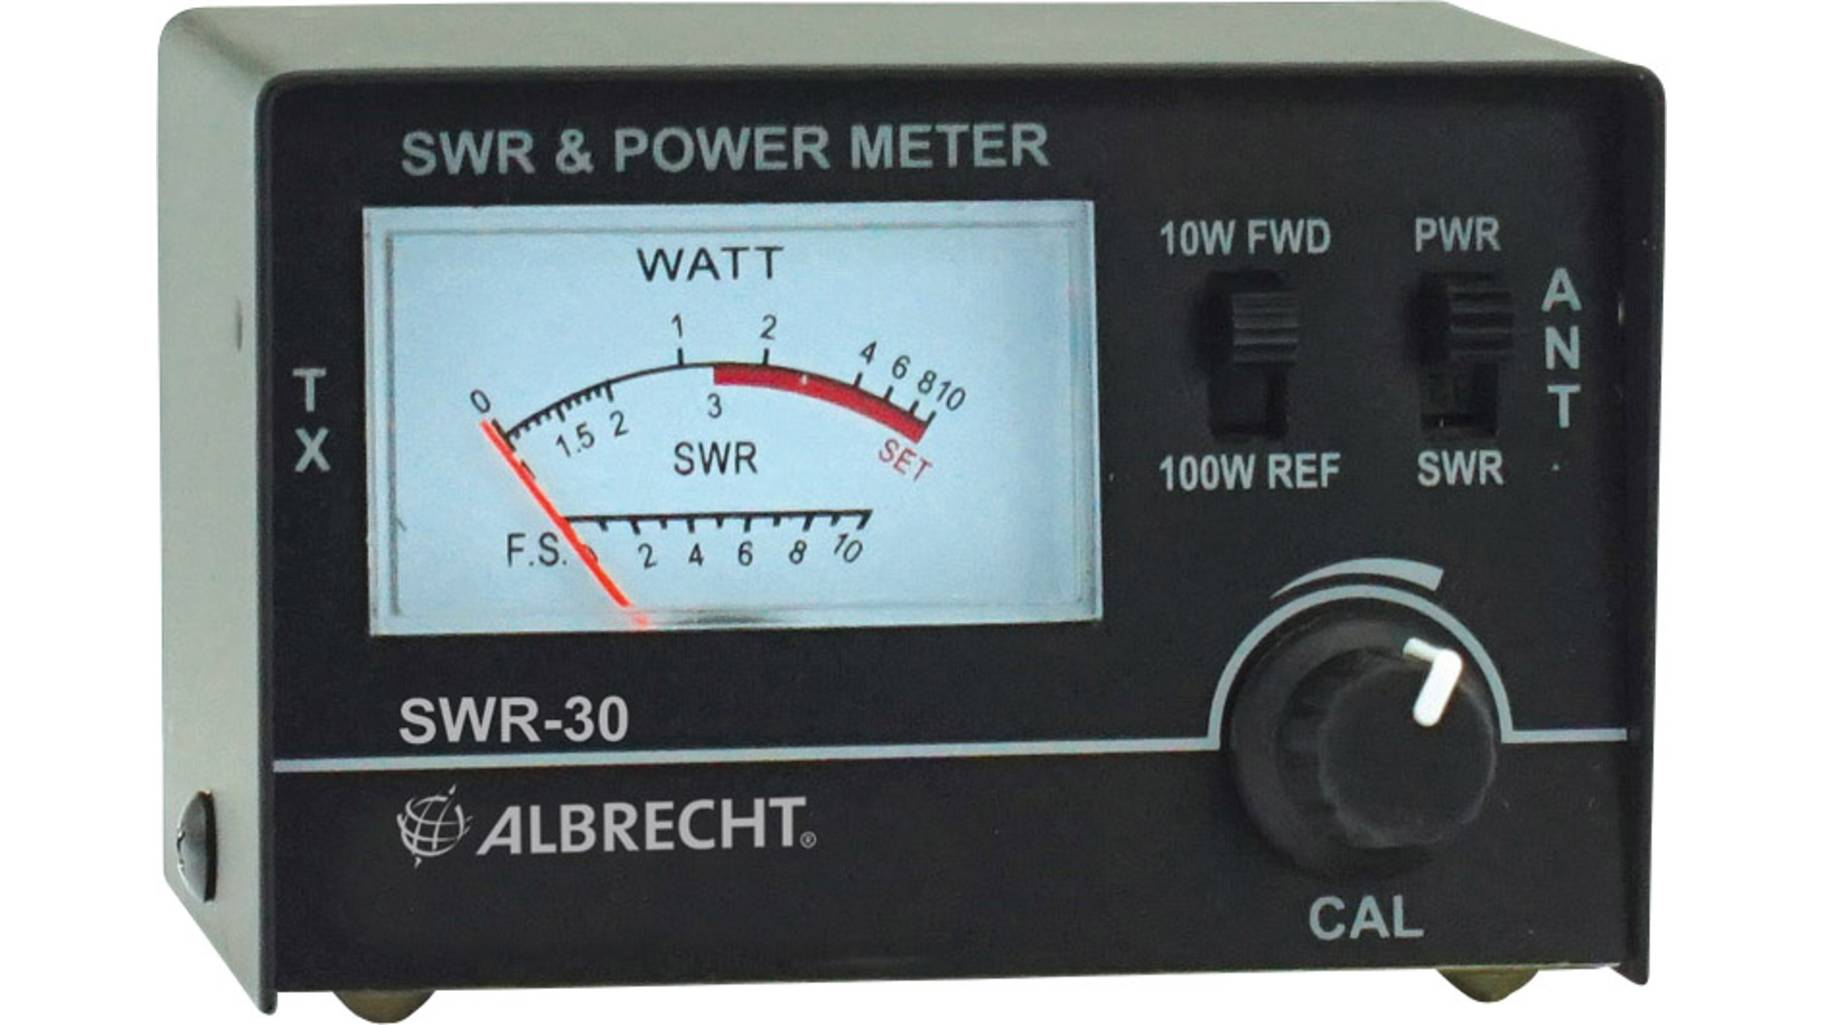
\includegraphics[width=0.85\textwidth]{foto/144}
    \caption{\scriptsize Ein einfaches SWR-Meter zum Bestimmen des Stehwellenverhältnisses}
    \label{swr_meter}
\end{figure}

    \end{column}
   \begin{column}{0.48\textwidth}
       
\begin{figure}
    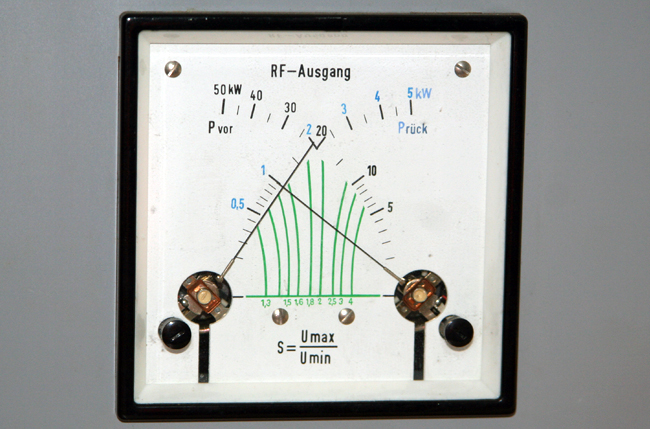
\includegraphics[width=0.85\textwidth]{foto/143}
    \caption{\scriptsize SWR-Meter mit Kreuzzeiger, linker Zeiger für die vorlaufende und rechter Zeiger für die rücklaufende Leistung; um das SWR abzulesen wird der grünen Linie am Schnittpunkt beider Zeiger nach unten gefolgt}
    \label{swr_meter_kreuzzeiger}
\end{figure}

   \end{column}
\end{columns}

\end{frame}

\begin{frame}Wird zwischen Transceiver und Antenne eingeschleift oder ist bereits im Transceiver eingebaut
\begin{columns}
    \begin{column}{0.48\textwidth}
    
\begin{figure}
    \DARCimage{0.85\linewidth}{670include}
    \caption{\scriptsize Prinzipbild SWR-Meter zwischen Transceiver  und Antenne}
    \label{n_trx_kabel_swr_antenne}
\end{figure}


    \end{column}
   \begin{column}{0.48\textwidth}
       
\begin{figure}
    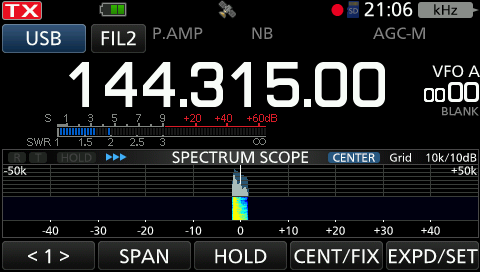
\includegraphics[width=0.85\textwidth]{foto/67}
    \caption{\scriptsize Display eines Transceivers}
    \label{n_swr_display}
\end{figure}

   \end{column}
\end{columns}

\end{frame}

\begin{frame}
\only<1>{
\begin{QQuestion}{NI201}{Mit welchem Messgerät lässt sich die Antennenanpassung bestimmen?}{Feldstärkemessgerät}
{Multimeter}
{Frequenzzähler}
{Stehwellenmessgerät}
\end{QQuestion}

}
\only<2>{
\begin{QQuestion}{NI201}{Mit welchem Messgerät lässt sich die Antennenanpassung bestimmen?}{Feldstärkemessgerät}
{Multimeter}
{Frequenzzähler}
{\textbf{\textcolor{DARCgreen}{Stehwellenmessgerät}}}
\end{QQuestion}

}
\end{frame}

\begin{frame}
\only<1>{
\begin{PQuestion}{NF101}{Die Darstellung zeigt das Display eines Transceivers im Sendebetrieb. Wie wird die Anzeige 1 bezeichnet?}{Wasserfalldiagramm}
{S-Meter}
{Amplitudenspektrum}
{SWR-Meter}
{\DARCimage{1.0\linewidth}{578include}}\end{PQuestion}

}
\only<2>{
\begin{PQuestion}{NF101}{Die Darstellung zeigt das Display eines Transceivers im Sendebetrieb. Wie wird die Anzeige 1 bezeichnet?}{Wasserfalldiagramm}
{S-Meter}
{Amplitudenspektrum}
{\textbf{\textcolor{DARCgreen}{SWR-Meter}}}
{\DARCimage{1.0\linewidth}{578include}}\end{PQuestion}

}
 \end{frame}

\begin{frame}
\only<1>{
\begin{QQuestion}{NI202}{Wenn das SWR-Meter auf der einen Seite mit der Antenne verbunden ist, was muss dann auf der anderen Seite angeschlossen werden, um Reflexionen zu messen?}{Transceiver}
{Netzteil}
{Dummy Load}
{Antennenschalter}
\end{QQuestion}

}
\only<2>{
\begin{QQuestion}{NI202}{Wenn das SWR-Meter auf der einen Seite mit der Antenne verbunden ist, was muss dann auf der anderen Seite angeschlossen werden, um Reflexionen zu messen?}{\textbf{\textcolor{DARCgreen}{Transceiver}}}
{Netzteil}
{Dummy Load}
{Antennenschalter}
\end{QQuestion}

}
\end{frame}

\begin{frame}
\frametitle{Gute Anpassung}
\begin{itemize}
  \item Bei perfekter Anpassung wird der Wert 1 angezeigt
  \item Der beste erreichbare Wert
  \end{itemize}
\end{frame}

\begin{frame}
\only<1>{
\begin{QQuestion}{NG301}{Bei welchem Stehwellenverhältnis (SWR) ist eine Antenne am besten an die Speiseleitung angepasst?}{1}
{0}
{3}
{$\mathrm{\infty}$}
\end{QQuestion}

}
\only<2>{
\begin{QQuestion}{NG301}{Bei welchem Stehwellenverhältnis (SWR) ist eine Antenne am besten an die Speiseleitung angepasst?}{\textbf{\textcolor{DARCgreen}{1}}}
{0}
{3}
{$\mathrm{\infty}$}
\end{QQuestion}

}
\end{frame}

\begin{frame}
\only<1>{
\begin{QQuestion}{NI203}{Ein Stehwellenmessgerät wird in ein ideal angepasstes Sender-/Antennensystem eingeschleift. Das Messgerät sollte~...}{ein Stehwellenverhältnis von 0 anzeigen.}
{einen Rücklauf von \qty{100}{\percent} anzeigen.}
{ein Stehwellenverhältnis von 1 anzeigen.}
{ein Stehwellenverhältnis von unendlich ($\mathrm{\infty}$) anzeigen.}
\end{QQuestion}

}
\only<2>{
\begin{QQuestion}{NI203}{Ein Stehwellenmessgerät wird in ein ideal angepasstes Sender-/Antennensystem eingeschleift. Das Messgerät sollte~...}{ein Stehwellenverhältnis von 0 anzeigen.}
{einen Rücklauf von \qty{100}{\percent} anzeigen.}
{\textbf{\textcolor{DARCgreen}{ein Stehwellenverhältnis von 1 anzeigen.}}}
{ein Stehwellenverhältnis von unendlich ($\mathrm{\infty}$) anzeigen.}
\end{QQuestion}

}
\end{frame}

\begin{frame}
\frametitle{Schlechte Anpassung}
\begin{itemize}
  \item Bei schlechter Anpassung wird nahe unendlich angezeigt
  \item Schlechte Anpassung an Übertragungsleitung
  \item Schlechte Anpassung an Antenne
  \item Defekte Übertragungsleitung
  \end{itemize}
\end{frame}

\begin{frame}
\only<1>{
\begin{PQuestion}{NG302}{Worauf deutet die dargestellte Anzeige des SWR-Meters hin?}{Eine zu hohe Sendeleistung}
{Eine gut angepasste Antenne}
{Eine schlecht angepasste Antenne}
{Eine zu geringe Sendeleistung}
{\DARCimage{1.0\linewidth}{580include}}\end{PQuestion}

}
\only<2>{
\begin{PQuestion}{NG302}{Worauf deutet die dargestellte Anzeige des SWR-Meters hin?}{Eine zu hohe Sendeleistung}
{Eine gut angepasste Antenne}
{\textbf{\textcolor{DARCgreen}{Eine schlecht angepasste Antenne}}}
{Eine zu geringe Sendeleistung}
{\DARCimage{1.0\linewidth}{580include}}\end{PQuestion}

}
\end{frame}

\begin{frame}
\only<1>{
\begin{QQuestion}{NG303}{Fehlanpassungen oder Beschädigungen von HF-Übertragungsleitungen führen~...}{zu Reflexionen des übertragenen HF-Signals und einem erhöhten SWR.}
{zu einer Überbeanspruchung der angeschlossenen Antenne.}
{zu einem SWR von kleiner oder gleich 1.}
{zur Erzeugung unerwünschter Aussendungen, da innerhalb der erforderlichen Bandbreite keine Anpassung gegeben ist.}
\end{QQuestion}

}
\only<2>{
\begin{QQuestion}{NG303}{Fehlanpassungen oder Beschädigungen von HF-Übertragungsleitungen führen~...}{\textbf{\textcolor{DARCgreen}{zu Reflexionen des übertragenen HF-Signals und einem erhöhten SWR.}}}
{zu einer Überbeanspruchung der angeschlossenen Antenne.}
{zu einem SWR von kleiner oder gleich 1.}
{zur Erzeugung unerwünschter Aussendungen, da innerhalb der erforderlichen Bandbreite keine Anpassung gegeben ist.}
\end{QQuestion}

}
\end{frame}

\begin{frame}
\frametitle{Hohe Kabeldämpfung}
\begin{itemize}
  \item Verringert das reflektierte Signal
  \item Führt zur Verfälschung der Messung
  \end{itemize}
\end{frame}

\begin{frame}
\only<1>{
\begin{QQuestion}{NG208}{Das koaxiale \qty{50}{\ohm}-Antennenkabel der \qty{2}{\m}-Amateurfunkstation wird mit einem gleichwertigen Koaxialkabel verlängert. Die Messung des SWR ergibt nach der Verlängerung einen besseren Wert. Was schließen Sie daraus? Durch die Verlängerung wird...}{die Dämpfung erhöht und das reflektierte Signal verstärkt}
{die Dämpfung verringert und das reflektierte Signal verstärkt.}
{die Dämpfung erhöht und das reflektierte Signal verringert.}
{die Dämpfung verringert und das reflektierte Signal verringert.}
\end{QQuestion}

}
\only<2>{
\begin{QQuestion}{NG208}{Das koaxiale \qty{50}{\ohm}-Antennenkabel der \qty{2}{\m}-Amateurfunkstation wird mit einem gleichwertigen Koaxialkabel verlängert. Die Messung des SWR ergibt nach der Verlängerung einen besseren Wert. Was schließen Sie daraus? Durch die Verlängerung wird...}{die Dämpfung erhöht und das reflektierte Signal verstärkt}
{die Dämpfung verringert und das reflektierte Signal verstärkt.}
{\textbf{\textcolor{DARCgreen}{die Dämpfung erhöht und das reflektierte Signal verringert.}}}
{die Dämpfung verringert und das reflektierte Signal verringert.}
\end{QQuestion}

}

\end{frame}%ENDCONTENT


\section{Personenschutz}
\label{section:personenschutzabstand}
\begin{frame}%STARTCONTENT
\begin{itemize}
  \item Elektromagnetische Felder können eine Auswirkung auf Menschen haben, die sich darin aufhalten
  \item Es darf zu keiner Gefährdung von Menschen durch Amateurfunkanlagen kommen
  \item \emph{Jeder Funkamateur} muss sich mit dem \emph{Personenschutz in elektromagnetischen Feldern} auskennen
  \end{itemize}

\end{frame}

\begin{frame}
\only<1>{
\begin{QQuestion}{NK201}{Warum muss ein Funkamateur Kenntnisse zum Personenschutz in elektromagnetischen Feldern haben?}{Damit er seinen Sender optimal an die Antenne anpassen kann.}
{Weil zu hohe Feldstärken in Antennennähe schädigend auf den menschlichen Körper wirken können.}
{Damit er bei einem Stromunfall als Ersthelfer tätig werden kann.}
{Weil eine Standortbescheinigung der Bundesnetzagentur hierfür nicht gültig wäre.}
\end{QQuestion}

}
\only<2>{
\begin{QQuestion}{NK201}{Warum muss ein Funkamateur Kenntnisse zum Personenschutz in elektromagnetischen Feldern haben?}{Damit er seinen Sender optimal an die Antenne anpassen kann.}
{\textbf{\textcolor{DARCgreen}{Weil zu hohe Feldstärken in Antennennähe schädigend auf den menschlichen Körper wirken können.}}}
{Damit er bei einem Stromunfall als Ersthelfer tätig werden kann.}
{Weil eine Standortbescheinigung der Bundesnetzagentur hierfür nicht gültig wäre.}
\end{QQuestion}

}
\end{frame}

\begin{frame}
\frametitle{EMVU}
Der Betreiber der ortsfesten Amateurfunkstelle ist für die Sicherstellung der \enquote{elektromagnetischen Verträglichkeit in der Umwelt} (EMVU) verantwortlich.

\end{frame}

\begin{frame}
\only<1>{
\begin{QQuestion}{VE501}{Was bedeutet die Abkürzung EMVU?}{Elektromagnetische Verträglichkeit in der Umwelt}
{Elektromagnetische Verträglichkeit von Geräten}
{Elektronische Messung von elektromagnetischen Unverträglichkeiten}
{Eine Bürgerinitiative zum Schutz vor elektromagnetischen Unverträglichkeiten}
\end{QQuestion}

}
\only<2>{
\begin{QQuestion}{VE501}{Was bedeutet die Abkürzung EMVU?}{\textbf{\textcolor{DARCgreen}{Elektromagnetische Verträglichkeit in der Umwelt}}}
{Elektromagnetische Verträglichkeit von Geräten}
{Elektronische Messung von elektromagnetischen Unverträglichkeiten}
{Eine Bürgerinitiative zum Schutz vor elektromagnetischen Unverträglichkeiten}
\end{QQuestion}

}
\end{frame}

\begin{frame}
\only<1>{
\begin{QQuestion}{VE502}{Wer ist für die Sicherstellung der elektromagnetischen Umweltverträglichkeit verantwortlich?}{Der Hersteller des Amateurfunkgerätes}
{Die Bundesnetzagentur}
{Der Betreiber der ortsfesten Amateurfunkstelle}
{Der Erbauer der Antennenanlage}
\end{QQuestion}

}
\only<2>{
\begin{QQuestion}{VE502}{Wer ist für die Sicherstellung der elektromagnetischen Umweltverträglichkeit verantwortlich?}{Der Hersteller des Amateurfunkgerätes}
{Die Bundesnetzagentur}
{\textbf{\textcolor{DARCgreen}{Der Betreiber der ortsfesten Amateurfunkstelle}}}
{Der Erbauer der Antennenanlage}
\end{QQuestion}

}
\end{frame}

\begin{frame}
\frametitle{BIm-SchV und BEMFV}
\begin{itemize}
  \item Grenzwerte finden sich in der \enquote{26. Verordnung zur Durchführung des Bundes-Immissionsschutzgesetzes} (26. BIm-SchV) und in der \enquote{Verordnung über das Nachweisverfahren zur Begrenzung elektromagnetischer Felder} (BEMFV)
  \item In der Verordnung über das \enquote{Nachweisverfahren zur Begrenzung elektromagnetischer Felder} (BEMFV) ist das Anzeigeverfahren beschrieben
  \item \emph{Funkamateur stellt vor Inbetriebnahme eigenständig sicher und dokumentiert, dass keine Gefährdung für Personen besteht}
  \end{itemize}

\end{frame}

\begin{frame}
\only<1>{
\begin{QQuestion}{VE505}{Wo sind die Grenzwerte zum Schutz von Personen und aktiven Körperhilfen in elektromagnetischen Feldern festgelegt?}{Im Gesetz über die Bereitstellung von Funkanlagen auf dem Markt (Funkanlagengesetz - FuAG) und im Telekommunikationsgesetz (TKG)}
{In der Richtlinie Elektromagnetische Verträglichkeit von Elektro- und Elektronikprodukten (EMV-Richtlinie) und im Gesetz über die elektromagnetische Verträglichkeit von Betriebsmitteln (EMVG)}
{In der 26. Verordnung zur Durchführung des Bundes-Immissionsschutzgesetzes (Verordnung über elektromagnetische Felder - 26. BImSchV) und in der Verordnung über das Nachweisverfahren zur Begrenzung elektromagnetischer Felder (BEMFV)}
{Im Gesetz über den Amateurfunk (Amateurfunkgesetz - AFuG) und in der Verordnung zum Gesetz über den Amateurfunk (Amateurfunkverordnung - AFuV)}
\end{QQuestion}

}
\only<2>{
\begin{QQuestion}{VE505}{Wo sind die Grenzwerte zum Schutz von Personen und aktiven Körperhilfen in elektromagnetischen Feldern festgelegt?}{Im Gesetz über die Bereitstellung von Funkanlagen auf dem Markt (Funkanlagengesetz - FuAG) und im Telekommunikationsgesetz (TKG)}
{In der Richtlinie Elektromagnetische Verträglichkeit von Elektro- und Elektronikprodukten (EMV-Richtlinie) und im Gesetz über die elektromagnetische Verträglichkeit von Betriebsmitteln (EMVG)}
{\textbf{\textcolor{DARCgreen}{In der 26. Verordnung zur Durchführung des Bundes-Immissionsschutzgesetzes (Verordnung über elektromagnetische Felder - 26. BImSchV) und in der Verordnung über das Nachweisverfahren zur Begrenzung elektromagnetischer Felder (BEMFV)}}}
{Im Gesetz über den Amateurfunk (Amateurfunkgesetz - AFuG) und in der Verordnung zum Gesetz über den Amateurfunk (Amateurfunkverordnung - AFuV)}
\end{QQuestion}

}
\end{frame}

\begin{frame}
\only<1>{
\begin{QQuestion}{VE503}{In welcher gesetzlichen Regelung ist das Verfahren zum Schutz von Personen in elektromagnetischen Feldern ortsfester Amateurfunkstellen festgelegt?}{Im Bundesimmissionsschutzgesetz (BImSchG)}
{Im Amateurfunkgesetz (AfuG)}
{In den Radio Regulations (RR)}
{In der Verordnung über das Nachweisverfahren zur Begrenzung elektromagnetischer Felder (BEMFV)}
\end{QQuestion}

}
\only<2>{
\begin{QQuestion}{VE503}{In welcher gesetzlichen Regelung ist das Verfahren zum Schutz von Personen in elektromagnetischen Feldern ortsfester Amateurfunkstellen festgelegt?}{Im Bundesimmissionsschutzgesetz (BImSchG)}
{Im Amateurfunkgesetz (AfuG)}
{In den Radio Regulations (RR)}
{\textbf{\textcolor{DARCgreen}{In der Verordnung über das Nachweisverfahren zur Begrenzung elektromagnetischer Felder (BEMFV)}}}
\end{QQuestion}

}
\end{frame}

\begin{frame}
\only<1>{
\begin{QQuestion}{VE504}{Was versteht man nach der Verordnung über das Nachweisverfahren zur Begrenzung elektromagnetischer Felder (BEMFV) unter dem \glqq Anzeigeverfahren ortsfester Amateurfunkanlagen\grqq{}?}{Die Erklärung des Funkamateurs, dass er den Grenzwert von \qty{10}{\W} EIRP unterschreitet}
{Ein Verfahren, das ein zertifiziertes Messlabor durchführen muss, um sicherzustellen, dass keine Gefährdung für Personen besteht}
{Ein Verfahren, das es dem Funkamateur ermöglicht, eigenständig sicherzustellen und zu dokumentieren, dass keine Gefährdung für Personen besteht}
{Die Erklärung des Funkamateurs, dass er den Grenzwert von \qty{750}{\W} PEP nicht überschreitet}
\end{QQuestion}

}
\only<2>{
\begin{QQuestion}{VE504}{Was versteht man nach der Verordnung über das Nachweisverfahren zur Begrenzung elektromagnetischer Felder (BEMFV) unter dem \glqq Anzeigeverfahren ortsfester Amateurfunkanlagen\grqq{}?}{Die Erklärung des Funkamateurs, dass er den Grenzwert von \qty{10}{\W} EIRP unterschreitet}
{Ein Verfahren, das ein zertifiziertes Messlabor durchführen muss, um sicherzustellen, dass keine Gefährdung für Personen besteht}
{\textbf{\textcolor{DARCgreen}{Ein Verfahren, das es dem Funkamateur ermöglicht, eigenständig sicherzustellen und zu dokumentieren, dass keine Gefährdung für Personen besteht}}}
{Die Erklärung des Funkamateurs, dass er den Grenzwert von \qty{750}{\W} PEP nicht überschreitet}
\end{QQuestion}

}
\end{frame}

\begin{frame}
\only<1>{
\begin{QQuestion}{VE511}{Welchen Status hat im Rahmen der EMVU die Anzeige einer ortsfesten Amateurfunkanlage?}{Die Anzeige ist die verbindliche Erklärung eines Funkamateurs über die eigenverantwortliche Einhaltung der gesetzlichen Grenzwerte zum Schutz von Personen in elektromagnetischen Feldern.}
{Die Anzeige ist eine unverbindliche Erklärung darüber, dass Funkamateure eigenverantwortlich handeln.}
{Die Anzeige hat den gleichen rechtlichen Status wie eine Standortbescheinigung, gilt aber nur für nichtkommerzielle Anlagen.}
{Die Anzeige ist die verbindliche Erklärung eines Funkamateurs über die eigenverantwortliche Einhaltung des Bundesimmissionsschutzgesetzes.}
\end{QQuestion}

}
\only<2>{
\begin{QQuestion}{VE511}{Welchen Status hat im Rahmen der EMVU die Anzeige einer ortsfesten Amateurfunkanlage?}{\textbf{\textcolor{DARCgreen}{Die Anzeige ist die verbindliche Erklärung eines Funkamateurs über die eigenverantwortliche Einhaltung der gesetzlichen Grenzwerte zum Schutz von Personen in elektromagnetischen Feldern.}}}
{Die Anzeige ist eine unverbindliche Erklärung darüber, dass Funkamateure eigenverantwortlich handeln.}
{Die Anzeige hat den gleichen rechtlichen Status wie eine Standortbescheinigung, gilt aber nur für nichtkommerzielle Anlagen.}
{Die Anzeige ist die verbindliche Erklärung eines Funkamateurs über die eigenverantwortliche Einhaltung des Bundesimmissionsschutzgesetzes.}
\end{QQuestion}

}
\end{frame}%ENDCONTENT


\section{Effektive Strahlungsleistung (ERP)}
\label{section:effektive_strahlungsleistung_erp_1}
\begin{frame}%STARTCONTENT
Kurze Wiederholung zu Antennen:
\begin{columns}
    \begin{column}{0.48\textwidth}
    Groundplane-Antenne strahlt in alle Himmelsrichtungen nahezu gleichmäßig ab, aber nicht nach oben oder unten


    \end{column}
   \begin{column}{0.48\textwidth}
       Yagi-Uda-Antenne bündelt die Funkstrahlen nach vorn und reduziert in alle anderen Richtungen


   \end{column}
\end{columns}
    \pause
    Bei der Berechnung der Grenzwerte für den Schutzabstand wird die \emph{Hauptstrahlrichtung} verwendet



\end{frame}

\begin{frame}
\frametitle{Gewinnfaktor}
\begin{itemize}
  \item Wie viel besser eine Antenne in Hauptstrahlrichtung im Vergleich zu einem Halbwellendipol abstrahlt
  \item Gewinnfaktor 2: Antenne strahlt in Hauptstrahlrichtung doppelt so stark wie ein Halbwellendipol in seine Hauptstrahlrichtung
  \end{itemize}

\end{frame}

\begin{frame}
\frametitle{Effektive Strahlungsleistung (ERP)}
Sendeleistung zur Antenne multipliziert mit Gewinnfaktor
    \pause
    Beispiel: 5~W auf eine Antenne mit Gewinnfaktor 2 ergibt die effektive Strahlungsleistung von 10~W

\end{frame}

\begin{frame}
\only<1>{
\begin{QQuestion}{NG401}{Die effektive Strahlungsleistung ERP (Effective Radiated Power) ist die von~...}{einem isotropen Strahler abgestrahlte Leistung, bezogen auf eine Antenne.}
{einer Antenne abgestrahlte Leistung, bezogen auf einen isotropen Strahler.}
{einem Halbwellendipol abgestrahlte Leistung, bezogen auf eine Antenne.}
{einer Antenne abgestrahlte Leistung, bezogen auf einen Halbwellendipol.}
\end{QQuestion}

}
\only<2>{
\begin{QQuestion}{NG401}{Die effektive Strahlungsleistung ERP (Effective Radiated Power) ist die von~...}{einem isotropen Strahler abgestrahlte Leistung, bezogen auf eine Antenne.}
{einer Antenne abgestrahlte Leistung, bezogen auf einen isotropen Strahler.}
{einem Halbwellendipol abgestrahlte Leistung, bezogen auf eine Antenne.}
{\textbf{\textcolor{DARCgreen}{einer Antenne abgestrahlte Leistung, bezogen auf einen Halbwellendipol.}}}
\end{QQuestion}

}
\end{frame}%ENDCONTENT


\section{Äquivalente isotrope Strahlungsleistung (EIRP)}
\label{section:aequivalente_isotrope_strahlungsleistung_eirp_1}
\begin{frame}%STARTCONTENT

\frametitle{Kugelstrahler oder Isotroper Strahler}
\begin{columns}
    \begin{column}{0.48\textwidth}
    
\begin{figure}
    \DARCimage{0.85\linewidth}{751include}
    \caption{\scriptsize Isotroper Strahler in der Mitte einer Kugel, der an allen Stellen der Kugeloberfläche die gleiche Strahlungsleistung erzeugt}
    \label{n_Kugelstrahler}
\end{figure}


    \end{column}
   \begin{column}{0.48\textwidth}
       \begin{itemize}
  \item Theoretische Antenne
  \item Unendlich klein
  \item Funkwellen werden gleichmäßig in alle Richtungen abgestrahlt
  \item Es existiert keine Hauptstrahlrichtung
  \end{itemize}

   \end{column}
\end{columns}

\end{frame}

\begin{frame}
\frametitle{EIRP}
\begin{itemize}
  \item Bei Berechnung der Strahlungsleistung in Bezug zum isotropen Strahler wird von \enquote{äquivalenter isotroper Strahlungsleistung} gesprochen
  \item Englisch \enquote{equivalent isotropic radiated power} (EIRP)
  \end{itemize}
\end{frame}

\begin{frame}
\frametitle{Berechnung}
\begin{itemize}
  \item Erfolgt gleich zu ERP
  \item Hat eine Antennen einen Gewinnfaktor von 3 bezogen auf den isotropen Strahler, dann strahlt diese Antenne in Hauptstrahlrichtung dreimal so stark wie ein isotroper Strahler in jede beliebige Richtung
  \item Bei 5~W Sendeleistung auf Antenne mit Gewinnfaktor 3 gegenüber dem isotropen Strahler ergibt das die Strahlungsleistung 15~W EIRP
  \end{itemize}
\end{frame}

\begin{frame}
\frametitle{Bezug zum Halbwellendipol}
\begin{itemize}
  \item Halbwellendipol hat den Gewinnfaktor 1,64 gegenüber isotropen Strahler
  \item Antenne mit Gewinnfaktor 2 gegenüber Halbwellendipol hat einen Gewinnfaktor von 2 $\cdot$ 1,64 = 3,28 gegenüber isotropen Strahler
  \end{itemize}
\end{frame}

\begin{frame}
\only<1>{
\begin{QQuestion}{NG402}{Die gleichwertige isotrope Strahlungsleistung EIRP (Equivalent Isotropic Radiated Power) ist die von~...}{einem isotropen Strahler abgestrahlte Leistung, bezogen auf eine Antenne.}
{einer Antenne abgestrahlte Leistung, bezogen auf einen Halbwellendipol.}
{einem Halbwellendipol abgestrahlte Leistung, bezogen auf eine Antenne.}
{einer Antenne abgestrahlte Leistung, bezogen auf einen isotropen Strahler.}
\end{QQuestion}

}
\only<2>{
\begin{QQuestion}{NG402}{Die gleichwertige isotrope Strahlungsleistung EIRP (Equivalent Isotropic Radiated Power) ist die von~...}{einem isotropen Strahler abgestrahlte Leistung, bezogen auf eine Antenne.}
{einer Antenne abgestrahlte Leistung, bezogen auf einen Halbwellendipol.}
{einem Halbwellendipol abgestrahlte Leistung, bezogen auf eine Antenne.}
{\textbf{\textcolor{DARCgreen}{einer Antenne abgestrahlte Leistung, bezogen auf einen isotropen Strahler.}}}
\end{QQuestion}

}
\end{frame}%ENDCONTENT


\section{Sendeleistung Klasse N}
\label{section:sendeleistung_klasse_n}
\begin{frame}%STARTCONTENT
\begin{itemize}
  \item 10~m-Band: 10~W ERP
  \item 2~m- und 70~cm-Band: 10~W EIRP
  \end{itemize}
    \pause
    Ein Funkgerät mit 5W Sendeleistung und einem Gewinnfaktor von 1,8 bezogen auf den isotropen Kugelstrahler darf damit betrieben werden:<br/>5~W $\cdot$ 1,8 = 9~W

\end{frame}

\begin{frame}
\only<1>{
\begin{QQuestion}{VD724}{Wie hoch ist die maximal zulässige isotrope Strahlungsleistung (EIRP) für Funkamateure mit der Zulassungsklasse~N im \qty{2}{\m}- und \qty{70}{\cm}-Band?}{\qty{100}{\W}}
{\qty{5}{\W}}
{\qty{10}{\W}}
{\qty{25}{\W}}
\end{QQuestion}

}
\only<2>{
\begin{QQuestion}{VD724}{Wie hoch ist die maximal zulässige isotrope Strahlungsleistung (EIRP) für Funkamateure mit der Zulassungsklasse~N im \qty{2}{\m}- und \qty{70}{\cm}-Band?}{\qty{100}{\W}}
{\qty{5}{\W}}
{\textbf{\textcolor{DARCgreen}{\qty{10}{\W}}}}
{\qty{25}{\W}}
\end{QQuestion}

}
\end{frame}

\begin{frame}
\only<1>{
\begin{QQuestion}{VD743}{Wie hoch ist die maximal zulässige effektive Strahlungsleistung (ERP) für Funkamateure mit der Zulassungsklasse~N im \qty{10}{\m}-Band?}{\qty{100}{\W}}
{\qty{5}{\W}}
{\qty{10}{\W}}
{\qty{25}{\W}}
\end{QQuestion}

}
\only<2>{
\begin{QQuestion}{VD743}{Wie hoch ist die maximal zulässige effektive Strahlungsleistung (ERP) für Funkamateure mit der Zulassungsklasse~N im \qty{10}{\m}-Band?}{\qty{100}{\W}}
{\qty{5}{\W}}
{\textbf{\textcolor{DARCgreen}{\qty{10}{\W}}}}
{\qty{25}{\W}}
\end{QQuestion}

}
\end{frame}

\begin{frame}
\only<1>{
\begin{QQuestion}{VD726}{Sie sind Inhaber einer Zulassung für den Amateurfunkdienst der Klasse N und nutzen ein Funkgerät mit 5 W Senderausgangsleistung. Dürfen Sie bei Sendebetrieb im \qty{2}{\m}-Band eine direkt angeschlossene Antenne mit Gewinnfaktor 1,8 bezogen auf den isotropen Kugelstrahler (entspricht 2,6 dBi Gewinn) verwenden?}{Nein, da sich eine Strahlungsleistung von über 10 W EIRP ergibt.}
{Ja, außer wenn die Amateurfunkstelle ortsfest betrieben wird.}
{Ja, da die Strahlungsleistung den Grenzwert von 10 W EIRP nicht überschreitet.}
{Nein, da ich Antennen mit Gewinn nicht benutzen darf}
\end{QQuestion}

}
\only<2>{
\begin{QQuestion}{VD726}{Sie sind Inhaber einer Zulassung für den Amateurfunkdienst der Klasse N und nutzen ein Funkgerät mit 5 W Senderausgangsleistung. Dürfen Sie bei Sendebetrieb im \qty{2}{\m}-Band eine direkt angeschlossene Antenne mit Gewinnfaktor 1,8 bezogen auf den isotropen Kugelstrahler (entspricht 2,6 dBi Gewinn) verwenden?}{Nein, da sich eine Strahlungsleistung von über 10 W EIRP ergibt.}
{Ja, außer wenn die Amateurfunkstelle ortsfest betrieben wird.}
{\textbf{\textcolor{DARCgreen}{Ja, da die Strahlungsleistung den Grenzwert von 10 W EIRP nicht überschreitet.}}}
{Nein, da ich Antennen mit Gewinn nicht benutzen darf}
\end{QQuestion}

}
\end{frame}

\begin{frame}
\only<1>{
\begin{QQuestion}{VD725}{Sie sind Inhaber einer Zulassung für den Amateurfunkdienst der Klasse N und nutzen ein Funkgerät mit 5 W Senderausgangsleistung. Dürfen Sie bei Sendebetrieb im \qty{2}{\m}-Band eine direkt angeschlossene Antenne mit Gewinnfaktor 2,5 bezogen auf den isotropen Kugelstrahler (entspricht 4,0 dBi Gewinn) verwenden?}{Ja, da die Senderausgangsleistung den Grenzwert von 10 W EIRP nicht überschreitet.}
{Nein, da ich Antennen mit Gewinn nicht benutzen darf.}
{Nein, da sich eine Strahlungsleistung von über 10 W EIRP ergibt.}
{Ja, sofern es sich um ein Handfunkgerät handelt.}
\end{QQuestion}

}
\only<2>{
\begin{QQuestion}{VD725}{Sie sind Inhaber einer Zulassung für den Amateurfunkdienst der Klasse N und nutzen ein Funkgerät mit 5 W Senderausgangsleistung. Dürfen Sie bei Sendebetrieb im \qty{2}{\m}-Band eine direkt angeschlossene Antenne mit Gewinnfaktor 2,5 bezogen auf den isotropen Kugelstrahler (entspricht 4,0 dBi Gewinn) verwenden?}{Ja, da die Senderausgangsleistung den Grenzwert von 10 W EIRP nicht überschreitet.}
{Nein, da ich Antennen mit Gewinn nicht benutzen darf.}
{\textbf{\textcolor{DARCgreen}{Nein, da sich eine Strahlungsleistung von über 10 W EIRP ergibt.}}}
{Ja, sofern es sich um ein Handfunkgerät handelt.}
\end{QQuestion}

}
\end{frame}%ENDCONTENT


\section{Anzeige ortsfester Amateurfunkanlagen}
\label{section:anzeige_ortsfester_amateurfunkanlagen}
\begin{frame}%STARTCONTENT
Für ortsfeste Amateurfunkstellen muss das Nachweisverfahren nur dann durchgeführt werden, wenn die Sendeanlage eine Strahlungsleistung von \qty{10}{\watt} EIRP oder höher erreicht.

\end{frame}

\begin{frame}
\only<1>{
\begin{QQuestion}{VE508}{Wer muss seine Amateurfunkstelle bei der BNetzA gemäß der Verordnung über das Nachweisverfahren zur Begrenzung elektromagnetischer Felder (BEMFV) anzeigen?}{Alle Funkamateure der Zeugnisklasse A}
{Alle Funkamateure, die Portabel- bzw. Mobilbetrieb durchführen}
{Alle Funkamateure, die ortsfeste Amateurfunkstellen mit einer Leistung ab \qty{10}{\W} EIRP betreiben}
{Alle Funkamateure, die auf der Kurzwelle aktiv sind}
\end{QQuestion}

}
\only<2>{
\begin{QQuestion}{VE508}{Wer muss seine Amateurfunkstelle bei der BNetzA gemäß der Verordnung über das Nachweisverfahren zur Begrenzung elektromagnetischer Felder (BEMFV) anzeigen?}{Alle Funkamateure der Zeugnisklasse A}
{Alle Funkamateure, die Portabel- bzw. Mobilbetrieb durchführen}
{\textbf{\textcolor{DARCgreen}{Alle Funkamateure, die ortsfeste Amateurfunkstellen mit einer Leistung ab \qty{10}{\W} EIRP betreiben}}}
{Alle Funkamateure, die auf der Kurzwelle aktiv sind}
\end{QQuestion}

}
\end{frame}

\begin{frame}
\only<1>{
\begin{QQuestion}{VE507}{Für welche Amateurfunkstellen muss der Schutz von Personen in elektromagnetischen Feldern vom Funkamateur dokumentiert werden?}{Für alle ortsfesten Amateurfunkstellen ab einer äquivalenten isotropen Strahlungsleistung von \qty{10}{\W} EIRP}
{Für alle Amateurfunkstellen}
{Für alle ortsfesten Amateurfunkstellen}
{Für alle Amateurfunkstellen ab einer äquivalenten Strahlungsleistung von \qty{10}{\W} EIRP}
\end{QQuestion}

}
\only<2>{
\begin{QQuestion}{VE507}{Für welche Amateurfunkstellen muss der Schutz von Personen in elektromagnetischen Feldern vom Funkamateur dokumentiert werden?}{\textbf{\textcolor{DARCgreen}{Für alle ortsfesten Amateurfunkstellen ab einer äquivalenten isotropen Strahlungsleistung von \qty{10}{\W} EIRP}}}
{Für alle Amateurfunkstellen}
{Für alle ortsfesten Amateurfunkstellen}
{Für alle Amateurfunkstellen ab einer äquivalenten Strahlungsleistung von \qty{10}{\W} EIRP}
\end{QQuestion}

}
\end{frame}

\begin{frame}
\frametitle{Anzeige bei BNetzA}
\begin{itemize}
  \item vor der Aufnahme des Betriebs der ortsfesten Amateurfunkanlage
  \item bei zuständiger Außenstelle der BNetzA
  \end{itemize}
\end{frame}

\begin{frame}
\only<1>{
\begin{QQuestion}{VE509}{Bei welcher Stelle und zu welchem Zeitpunkt ist die Anzeige gemäß der Verordnung über das Nachweisverfahren zur Begrenzung elektromagnetischer Felder (BEMFV) für eine ortsfeste Amateurfunkanlage mit einer EIRP ab \qty{10}{\W} einzureichen?}{Die Anzeige ist spätestens drei Monate nach Betriebsaufnahme bei der zuständigen Außenstelle der BNetzA einzureichen.}
{Die Anzeige ist vor Aufnahme des Betriebs der Amateurfunkanlage bei der zuständigen Außenstelle der BNetzA einzureichen.}
{Wenn die Anzeige den tatsächlichen Gegebenheiten nicht mehr entspricht, ist dieses einer beliebigen Außenstelle der BNetzA mitzuteilen.}
{Die Anzeige ist bei einer beliebigen Außenstelle der BNetzA vor Aufnahme des Betriebs der Amateurfunkanlage einzureichen.}
\end{QQuestion}

}
\only<2>{
\begin{QQuestion}{VE509}{Bei welcher Stelle und zu welchem Zeitpunkt ist die Anzeige gemäß der Verordnung über das Nachweisverfahren zur Begrenzung elektromagnetischer Felder (BEMFV) für eine ortsfeste Amateurfunkanlage mit einer EIRP ab \qty{10}{\W} einzureichen?}{Die Anzeige ist spätestens drei Monate nach Betriebsaufnahme bei der zuständigen Außenstelle der BNetzA einzureichen.}
{\textbf{\textcolor{DARCgreen}{Die Anzeige ist vor Aufnahme des Betriebs der Amateurfunkanlage bei der zuständigen Außenstelle der BNetzA einzureichen.}}}
{Wenn die Anzeige den tatsächlichen Gegebenheiten nicht mehr entspricht, ist dieses einer beliebigen Außenstelle der BNetzA mitzuteilen.}
{Die Anzeige ist bei einer beliebigen Außenstelle der BNetzA vor Aufnahme des Betriebs der Amateurfunkanlage einzureichen.}
\end{QQuestion}

}
\end{frame}

\begin{frame}
\frametitle{Inhalt der Anzeige}
Nachvollziehbare zeichnerische Darstellung mit

\begin{itemize}
  \item Standortbezogener Sicherheitsabstand
  \item Vom Betreiber kontrollierbarer Bereich
  \end{itemize}
\end{frame}

\begin{frame}
\frametitle{Zusätzlich zur Anzeige}
An der Funkstation liegend und auf Verlangen der BNetzA vorzulegen:

\begin{itemize}
  \item Einhaltung der Anforderungen
  \item ggf. Antennendiagramme
  \item Lageplan
  \item Bauzeichnung oder Skizze mit Bemaßung
  \item Konfiguration der Funkanlage
  \end{itemize}
\end{frame}

\begin{frame}
\only<1>{
\begin{QQuestion}{VE512}{Welche Unterlagen sind ergänzend zur Anzeige gemäß der Verordnung über das Nachweisverfahren zur Begrenzung elektromagnetischer Felder (BEMFV) einer ortsfesten Amateurfunkanlage bei der zuständigen Außenstelle der BNetzA einzureichen?}{Es ist ein Blockschaltbild der Amateurfunkstelle beizufügen.}
{Der Anzeige sind Antennendiagramme, Lageplan, Bauzeichnung oder Skizze mit Bemaßung beizufügen.}
{Es sind keine weiteren Unterlagen beizufügen.}
{Der Anzeige ist eine nachvollziehbare zeichnerische Darstellung des standortbezogenen Sicherheitsabstands und des vom Betreiber kontrollierbaren Bereichs beizufügen.}
\end{QQuestion}

}
\only<2>{
\begin{QQuestion}{VE512}{Welche Unterlagen sind ergänzend zur Anzeige gemäß der Verordnung über das Nachweisverfahren zur Begrenzung elektromagnetischer Felder (BEMFV) einer ortsfesten Amateurfunkanlage bei der zuständigen Außenstelle der BNetzA einzureichen?}{Es ist ein Blockschaltbild der Amateurfunkstelle beizufügen.}
{Der Anzeige sind Antennendiagramme, Lageplan, Bauzeichnung oder Skizze mit Bemaßung beizufügen.}
{Es sind keine weiteren Unterlagen beizufügen.}
{\textbf{\textcolor{DARCgreen}{Der Anzeige ist eine nachvollziehbare zeichnerische Darstellung des standortbezogenen Sicherheitsabstands und des vom Betreiber kontrollierbaren Bereichs beizufügen.}}}
\end{QQuestion}

}
\end{frame}

\begin{frame}
\only<1>{
\begin{QQuestion}{VE513}{Welche Unterlagen hat der Funkamateur ergänzend zur Anzeige einer ortsfesten Amateurfunkanlage gemäß der Verordnung über das Nachweisverfahren zur Begrenzung elektromagnetischer Felder (BEMFV) ab dem Zeitpunkt der Inbetriebnahme bereitzuhalten und der Bundesnetzagentur nach Aufforderung vorzulegen?}{Eine nachvollziehbare Dokumentation über die Einhaltung der Anforderungen, gegebenenfalls Antennendiagramme, einen Lageplan, eine Bauzeichnung oder Skizze mit Bemaßung und die Konfiguration der Funkanlage}
{Das Anzeigeformblatt mit den Daten der ortsfesten Amateurfunkanlage und eine maßstäbliche Skizze des standortbezogenen Sicherheitsabstandes und des kontrollierbaren Bereiches}
{Die Zulassung zur Teilnahme am Amateurfunkdienst, die Datenblätter aller Amateurfunkgeräte und das Logbuch, denn sie müssen jederzeit für eine mögliche Kontrolle durch die Bundesnetzagentur verfügbar sein}
{Eine Fotodokumentation der Amateurfunkanlage einschließlich der Antennen sowie eine formlose Aufstellung aller Messwerte nebst Antennendiagrammen}
\end{QQuestion}

}
\only<2>{
\begin{QQuestion}{VE513}{Welche Unterlagen hat der Funkamateur ergänzend zur Anzeige einer ortsfesten Amateurfunkanlage gemäß der Verordnung über das Nachweisverfahren zur Begrenzung elektromagnetischer Felder (BEMFV) ab dem Zeitpunkt der Inbetriebnahme bereitzuhalten und der Bundesnetzagentur nach Aufforderung vorzulegen?}{\textbf{\textcolor{DARCgreen}{Eine nachvollziehbare Dokumentation über die Einhaltung der Anforderungen, gegebenenfalls Antennendiagramme, einen Lageplan, eine Bauzeichnung oder Skizze mit Bemaßung und die Konfiguration der Funkanlage}}}
{Das Anzeigeformblatt mit den Daten der ortsfesten Amateurfunkanlage und eine maßstäbliche Skizze des standortbezogenen Sicherheitsabstandes und des kontrollierbaren Bereiches}
{Die Zulassung zur Teilnahme am Amateurfunkdienst, die Datenblätter aller Amateurfunkgeräte und das Logbuch, denn sie müssen jederzeit für eine mögliche Kontrolle durch die Bundesnetzagentur verfügbar sein}
{Eine Fotodokumentation der Amateurfunkanlage einschließlich der Antennen sowie eine formlose Aufstellung aller Messwerte nebst Antennendiagrammen}
\end{QQuestion}

}
\end{frame}

\begin{frame}
\only<1>{
\begin{QQuestion}{VD107}{In welchem Fall hat ein Funkamateur der Bundesnetzagentur gemäß Amateurfunkverordnung (AFuV) technische Unterlagen über seine Sendeanlage vorzulegen?}{Auf Anforderung der Bundesnetzagentur}
{Bei jeder technischen Änderung an der Sendeanlage}
{Unverzüglich nach Erhalt der Amateurfunkzulassung}
{Bei Sendeleistungen größer als \qty{750}{\W}}
\end{QQuestion}

}
\only<2>{
\begin{QQuestion}{VD107}{In welchem Fall hat ein Funkamateur der Bundesnetzagentur gemäß Amateurfunkverordnung (AFuV) technische Unterlagen über seine Sendeanlage vorzulegen?}{\textbf{\textcolor{DARCgreen}{Auf Anforderung der Bundesnetzagentur}}}
{Bei jeder technischen Änderung an der Sendeanlage}
{Unverzüglich nach Erhalt der Amateurfunkzulassung}
{Bei Sendeleistungen größer als \qty{750}{\W}}
\end{QQuestion}

}
\end{frame}

\begin{frame}
\frametitle{Änderungen}
\begin{itemize}
  \item Fortlaufend prüfen, ob die Anlage gleich zu der in der Anzeige ist
  \item Bei wesentlichen Änderungen erneute Anzeige durchführen
  \end{itemize}
\end{frame}

\begin{frame}
\only<1>{
\begin{QQuestion}{VE514}{Was hat ein Funkamateur zu beachten, nachdem er seine ortsfeste Amateurfunkstelle bei der Bundesnetzagentur gemäß BEMFV angezeigt hat?}{Nachdem die ortsfeste Amateurfunkstelle in Betrieb genommen wurde, ist die Dokumentation über die Einhaltung der Anforderungen mit allen erforderlichen Unterlagen der zuständigen Außenstelle der Bundesnetzagentur vorzulegen.}
{Mit der Anzeige seiner ortsfesten Amateurfunkstelle ist ein Funkamateur seinen Verpflichtungen zum Schutz von Personen in elektromagnetischen Feldern nachgekommen und muss diesbezüglich nichts weiter beachten.}
{Das Anzeigeverfahren ist jedes Jahr erneut durchzuführen, um die Aktualität zu gewährleisten.}
{Er hat eine Dokumentation über die Einhaltung der Anforderungen mit allen erforderlichen Unterlagen bereitzuhalten und fortlaufend zu prüfen, ob die Bedingungen, unter denen die Anzeige durchgeführt wurde, noch zutreffend sind. Bei wesentlichen Änderungen ist die Amateurfunkstelle erneut anzuzeigen.}
\end{QQuestion}

}
\only<2>{
\begin{QQuestion}{VE514}{Was hat ein Funkamateur zu beachten, nachdem er seine ortsfeste Amateurfunkstelle bei der Bundesnetzagentur gemäß BEMFV angezeigt hat?}{Nachdem die ortsfeste Amateurfunkstelle in Betrieb genommen wurde, ist die Dokumentation über die Einhaltung der Anforderungen mit allen erforderlichen Unterlagen der zuständigen Außenstelle der Bundesnetzagentur vorzulegen.}
{Mit der Anzeige seiner ortsfesten Amateurfunkstelle ist ein Funkamateur seinen Verpflichtungen zum Schutz von Personen in elektromagnetischen Feldern nachgekommen und muss diesbezüglich nichts weiter beachten.}
{Das Anzeigeverfahren ist jedes Jahr erneut durchzuführen, um die Aktualität zu gewährleisten.}
{\textbf{\textcolor{DARCgreen}{Er hat eine Dokumentation über die Einhaltung der Anforderungen mit allen erforderlichen Unterlagen bereitzuhalten und fortlaufend zu prüfen, ob die Bedingungen, unter denen die Anzeige durchgeführt wurde, noch zutreffend sind. Bei wesentlichen Änderungen ist die Amateurfunkstelle erneut anzuzeigen.}}}
\end{QQuestion}

}
\end{frame}

\begin{frame}
\only<1>{
\begin{QQuestion}{VE510}{Wann ist erneut eine Anzeige einer ortsfesten Amateurfunkanlage gemäß der Verordnung über das Nachweisverfahren zur Begrenzung elektromagnetischer Felder (BEMFV) bei der zuständigen Stelle der BNetzA einzureichen?}{Die Anzeige ist jährlich zu aktualisieren. Wurden keine Änderungen an der Amateurfunkanlage vorgenommen, reicht eine formlose Mitteilung.}
{Wenn die bestehende Anzeige nicht mehr den tatsächlichen Gegebenheiten entspricht, ist vom Betreiber das Anzeigeverfahren erneut durchzuführen.}
{Bei einem Wechsel der nationalen Zeugnisklasse}
{Nach Aufforderung der zuständigen Stelle der BNetzA}
\end{QQuestion}

}
\only<2>{
\begin{QQuestion}{VE510}{Wann ist erneut eine Anzeige einer ortsfesten Amateurfunkanlage gemäß der Verordnung über das Nachweisverfahren zur Begrenzung elektromagnetischer Felder (BEMFV) bei der zuständigen Stelle der BNetzA einzureichen?}{Die Anzeige ist jährlich zu aktualisieren. Wurden keine Änderungen an der Amateurfunkanlage vorgenommen, reicht eine formlose Mitteilung.}
{\textbf{\textcolor{DARCgreen}{Wenn die bestehende Anzeige nicht mehr den tatsächlichen Gegebenheiten entspricht, ist vom Betreiber das Anzeigeverfahren erneut durchzuführen.}}}
{Bei einem Wechsel der nationalen Zeugnisklasse}
{Nach Aufforderung der zuständigen Stelle der BNetzA}
\end{QQuestion}

}
\end{frame}

\begin{frame}
\frametitle{Nachweisverfahren}
\begin{columns}
    \begin{column}{0.48\textwidth}
    \begin{itemize}
  \item Berechnung des Personen-Sicherheitsabstands
  \item Während des Sendebetriebs dürfen keine unbefugten Personen in diesem Bereich sein
  \item Ist erfüllt, wenn dieses im kontrollierbaren Bereich stattfindet, z.B. eigenes Grundstück
  \end{itemize}

    \end{column}
   \begin{column}{0.48\textwidth}
       Hilfsmittel:

\begin{itemize}
  \item Software \enquote{Watt Wächter (\textcolor{DARCblue}{\faLink~\href{https://50ohm.de/ww}{50ohm.de/ww}})}
  \item vereinfachtes Bewertungsverfahren
  \item Feldstärkemessung
  \item Fernfeldberechnung
  \item Nahfeldberechnung
  \end{itemize}

   \end{column}
\end{columns}

\end{frame}

\begin{frame}
\only<1>{
\begin{QQuestion}{VE506}{Was muss ein Funkamateur zum Schutz von Personen bei dem Betrieb von ortsfesten Amateurfunkanlagen gemäß der Verordnung über das Nachweisverfahren zur Begrenzung elektromagnetischer Felder (BEMFV) vornehmen?}{Er kann bei einer Leistung von bis zu \qty{100}{\W} PEP den standardisierten Sicherheitsabstand von \qty{25}{\m} annehmen.}
{Er kann bei einer Leistung von bis zu \qty{100}{\W} PEP den standardisierten Sicherheitsabstand von \qty{10}{\m} annehmen.}
{Er hat den zur Einhaltung der Grenzwerte erforderlichen Sicherheitsabstand einer Funkanlage mit EIRP von 10 W oder mehr rechnerisch oder messtechnisch zu ermitteln und in nachvollziehbarer Form zu dokumentieren.}
{Er hat den zur Einhaltung der Grenzwerte erforderlichen Sicherheitsabstand durch ein zertifiziertes Messlabor ermitteln zu lassen.}
\end{QQuestion}

}
\only<2>{
\begin{QQuestion}{VE506}{Was muss ein Funkamateur zum Schutz von Personen bei dem Betrieb von ortsfesten Amateurfunkanlagen gemäß der Verordnung über das Nachweisverfahren zur Begrenzung elektromagnetischer Felder (BEMFV) vornehmen?}{Er kann bei einer Leistung von bis zu \qty{100}{\W} PEP den standardisierten Sicherheitsabstand von \qty{25}{\m} annehmen.}
{Er kann bei einer Leistung von bis zu \qty{100}{\W} PEP den standardisierten Sicherheitsabstand von \qty{10}{\m} annehmen.}
{\textbf{\textcolor{DARCgreen}{Er hat den zur Einhaltung der Grenzwerte erforderlichen Sicherheitsabstand einer Funkanlage mit EIRP von 10 W oder mehr rechnerisch oder messtechnisch zu ermitteln und in nachvollziehbarer Form zu dokumentieren.}}}
{Er hat den zur Einhaltung der Grenzwerte erforderlichen Sicherheitsabstand durch ein zertifiziertes Messlabor ermitteln zu lassen.}
\end{QQuestion}

}
\end{frame}

\begin{frame}
\only<1>{
\begin{QQuestion}{VE515}{Welche Verfahren können Funkamateure nutzen, um den Nachweis zur Begrenzung von elektromagnetischen Feldern zu erstellen?}{Funkamateure sind ausdrücklich vom Nachweis zur Begrenzung von elektromagnetischen Feldern ausgenommen.}
{Funkamateure müssen eine zertifizierte Firma mit dem Nachweis zur Begrenzung von elektromagnetischen Feldern beauftragen.}
{Funkamateure können aufgrund ihrer Fachkenntnisse die Einhaltung der elektromagnetische Grenzwerte abschätzen.}
{Das Bewertungsverfahren mit der Anwendung \glqq Watt Wächter\grqq{}, das vereinfachte Bewertungsverfahren, Feldstärkemessung, Fernfeldberechnung und Nahfeldberechnung}
\end{QQuestion}

}
\only<2>{
\begin{QQuestion}{VE515}{Welche Verfahren können Funkamateure nutzen, um den Nachweis zur Begrenzung von elektromagnetischen Feldern zu erstellen?}{Funkamateure sind ausdrücklich vom Nachweis zur Begrenzung von elektromagnetischen Feldern ausgenommen.}
{Funkamateure müssen eine zertifizierte Firma mit dem Nachweis zur Begrenzung von elektromagnetischen Feldern beauftragen.}
{Funkamateure können aufgrund ihrer Fachkenntnisse die Einhaltung der elektromagnetische Grenzwerte abschätzen.}
{\textbf{\textcolor{DARCgreen}{Das Bewertungsverfahren mit der Anwendung \glqq Watt Wächter\grqq{}, das vereinfachte Bewertungsverfahren, Feldstärkemessung, Fernfeldberechnung und Nahfeldberechnung}}}
\end{QQuestion}

}
\end{frame}

\begin{frame}
\frametitle{Mehrere Aussendungen gleichzeitig}
\begin{itemize}
  \item Es können mehrere Funkamateure gleichzeitig an einer Anlage auf verschiedenen Frequenzen senden
  \item In der Regel über verschiedene Antennen
  \item Alle Antennen zusammen müssen für den Personenschutzabstand berücksichtigt werden
  \end{itemize}

\end{frame}

\begin{frame}
\only<1>{
\begin{QQuestion}{VE516}{Welche Aussendungen von Amateurfunkanlagen müssen bei der Ermittlung des standortbezogenen Sicherheitsabstandes berücksichtigt werden?}{Alle Aussendungen der ortsfesten Amateurfunkstelle, die ein Funkamateur zeitgleich durchzuführen beabsichtigt}
{Ausschließlich Aussendungen von ortsfest betriebenen Amateurfunkstellen mit einer Strahlungsleistung (EIRP) größer \qty{10}{\W}}
{Nur die Aussendungen der maximalen Sendeleistung, die die Amateurfunkanlage erbringen kann}
{Alle Aussendungen mit einer Strahlungsleistung (EIRP) größer \qty{10}{\W}, auch Aussendungen im Mobilbetrieb.}
\end{QQuestion}

}
\only<2>{
\begin{QQuestion}{VE516}{Welche Aussendungen von Amateurfunkanlagen müssen bei der Ermittlung des standortbezogenen Sicherheitsabstandes berücksichtigt werden?}{\textbf{\textcolor{DARCgreen}{Alle Aussendungen der ortsfesten Amateurfunkstelle, die ein Funkamateur zeitgleich durchzuführen beabsichtigt}}}
{Ausschließlich Aussendungen von ortsfest betriebenen Amateurfunkstellen mit einer Strahlungsleistung (EIRP) größer \qty{10}{\W}}
{Nur die Aussendungen der maximalen Sendeleistung, die die Amateurfunkanlage erbringen kann}
{Alle Aussendungen mit einer Strahlungsleistung (EIRP) größer \qty{10}{\W}, auch Aussendungen im Mobilbetrieb.}
\end{QQuestion}

}
\end{frame}

\begin{frame}
\only<1>{
\begin{QQuestion}{VE517}{Sie wollen eine Amateurfunkstelle mit mehreren Sendeantennen betreiben und die Personenschutz-Sicherheitsabstände ermitteln. Dabei ergibt sich, dass der Sicherheitsabstand mehrerer Antennen überlappt. Was müssen Sie nun beachten?}{Für die gesamte Antennenanlage gilt der Sicherheitsabstand der Antenne mit der größten Strahlungsleistung.}
{Die betroffenen Antennen sind gemeinsam zu betrachten, sofern mit ihnen gleichzeitig gesendet werden soll.}
{Es ist sicherzustellen, dass der Sendebetrieb zu jedem Zeitpunkt auf eine der Antennen beschränkt wird.}
{Die Sicherheitsabstände sind mit der Anzahl der Sendeantennen als Sicherheitsfaktor zu multiplizieren.}
\end{QQuestion}

}
\only<2>{
\begin{QQuestion}{VE517}{Sie wollen eine Amateurfunkstelle mit mehreren Sendeantennen betreiben und die Personenschutz-Sicherheitsabstände ermitteln. Dabei ergibt sich, dass der Sicherheitsabstand mehrerer Antennen überlappt. Was müssen Sie nun beachten?}{Für die gesamte Antennenanlage gilt der Sicherheitsabstand der Antenne mit der größten Strahlungsleistung.}
{\textbf{\textcolor{DARCgreen}{Die betroffenen Antennen sind gemeinsam zu betrachten, sofern mit ihnen gleichzeitig gesendet werden soll.}}}
{Es ist sicherzustellen, dass der Sendebetrieb zu jedem Zeitpunkt auf eine der Antennen beschränkt wird.}
{Die Sicherheitsabstände sind mit der Anzahl der Sendeantennen als Sicherheitsfaktor zu multiplizieren.}
\end{QQuestion}

}
\end{frame}%ENDCONTENT


\section{Standortbescheinigung}
\label{section:standortbescheinigung}
\begin{frame}%STARTCONTENT

\begin{columns}
    \begin{column}{0.48\textwidth}
    \begin{itemize}
  \item Eine Standortbescheinigung kann auf \emph{Antrag kostenpflichtig} durch die BNetzA ausgestellt werden
  \item Funkamateur muss alle notwendigen Unterlagen und Informationen für die Berechnung bereitstellen
  \end{itemize}

    \end{column}
   \begin{column}{0.48\textwidth}
       
    \pause
    \begin{itemize}
  \item Lageplan
  \item Bauzeichnung mit Montageort der Antennen
  \item Informationen zum Abstrahlverhalten von allen Antennen
  \end{itemize}



   \end{column}
\end{columns}

\end{frame}

\begin{frame}
\only<1>{
\begin{QQuestion}{VC121}{Kann der Funkamateur laut Amateurfunkgesetz (AFuG) eine Standortbescheinigung erhalten?}{Die Standortbescheinigung kann mit der IT-Anwendung \glqq Watt-Wächter\grqq{} erstellt werden.}
{Der Funkamateur kann auch auf Antrag keine Standortbescheinigung der BNetzA erhalten.}
{Die BNetzA stellt auf Antrag eine Standortbescheinigung aus.}
{Die BNetzA stellt mit der Zuteilung des Rufzeichens eine Standortbescheinigung aus.}
\end{QQuestion}

}
\only<2>{
\begin{QQuestion}{VC121}{Kann der Funkamateur laut Amateurfunkgesetz (AFuG) eine Standortbescheinigung erhalten?}{Die Standortbescheinigung kann mit der IT-Anwendung \glqq Watt-Wächter\grqq{} erstellt werden.}
{Der Funkamateur kann auch auf Antrag keine Standortbescheinigung der BNetzA erhalten.}
{\textbf{\textcolor{DARCgreen}{Die BNetzA stellt auf Antrag eine Standortbescheinigung aus.}}}
{Die BNetzA stellt mit der Zuteilung des Rufzeichens eine Standortbescheinigung aus.}
\end{QQuestion}

}
\end{frame}

\begin{frame}
\frametitle{Verpflichtende Standortbescheinigung}
Verpflichtend ist eine Standortbescheinigung, wenn sich am Standort der vorgesehenen ortsfesten Amateurfunkstelle bereits ortsfeste Funkanlagen befinden, die selbst eine Standortbescheinigung benötigen.

\end{frame}

\begin{frame}
\only<1>{
\begin{QQuestion}{VE519}{Kann die Bundesnetzagentur für den Betrieb einer ortsfesten Amateurfunkstelle eine Standortbescheinigung fordern?}{Nein, für Amateurfunkanlagen gilt das Anzeigeverfahren}
{Nur wenn sich am Standort der vorgesehenen ortsfesten Amateurfunkstelle bereits ortsfeste Funkanlagen befinden, die selbst eine Standortbescheinigung benötigen.}
{Nur wenn die Amateurfunkstelle gewerblich genutzt wird}
{Ja, wenn die effektive Strahlungsleistung der Amateurfunkstelle \qty{750}{\W} überschreitet}
\end{QQuestion}

}
\only<2>{
\begin{QQuestion}{VE519}{Kann die Bundesnetzagentur für den Betrieb einer ortsfesten Amateurfunkstelle eine Standortbescheinigung fordern?}{Nein, für Amateurfunkanlagen gilt das Anzeigeverfahren}
{\textbf{\textcolor{DARCgreen}{Nur wenn sich am Standort der vorgesehenen ortsfesten Amateurfunkstelle bereits ortsfeste Funkanlagen befinden, die selbst eine Standortbescheinigung benötigen.}}}
{Nur wenn die Amateurfunkstelle gewerblich genutzt wird}
{Ja, wenn die effektive Strahlungsleistung der Amateurfunkstelle \qty{750}{\W} überschreitet}
\end{QQuestion}

}
\end{frame}

\begin{frame}
\only<1>{
\begin{QQuestion}{VE518}{Sie wollen eine Amateurfunkstelle an einem Standort errichten, an dem sich bereits andere ortsfeste Funkanlagen befinden. Welche Besonderheit müssen Sie in Bezug auf den Schutz von Personen in elektromagnetischen Feldern beachten?}{Sofern die Senderausgangsleistung der Amateurfunkstelle 10 W überschreitet, darf sie an diesem Standort nicht betrieben werden.}
{Sofern die Gesamtleistung aller Funkanlagen am Standort 10 W EIRP erreicht oder überschreitet, ist eine Standortbescheinigung erforderlich.}
{Es ist unzulässig, eine Amateurfunkstelle an einem Standort zu betreiben, an dem sich auch Funkanlagen anderer Funkdienste befinden.}
{Es ist ein mechanischer Sendeumschalter erforderlich, der verhindert, dass die Amateurfunkanlage gleichzeitig mit einer der anderen Funkanlagen sendet.}
\end{QQuestion}

}
\only<2>{
\begin{QQuestion}{VE518}{Sie wollen eine Amateurfunkstelle an einem Standort errichten, an dem sich bereits andere ortsfeste Funkanlagen befinden. Welche Besonderheit müssen Sie in Bezug auf den Schutz von Personen in elektromagnetischen Feldern beachten?}{Sofern die Senderausgangsleistung der Amateurfunkstelle 10 W überschreitet, darf sie an diesem Standort nicht betrieben werden.}
{\textbf{\textcolor{DARCgreen}{Sofern die Gesamtleistung aller Funkanlagen am Standort 10 W EIRP erreicht oder überschreitet, ist eine Standortbescheinigung erforderlich.}}}
{Es ist unzulässig, eine Amateurfunkstelle an einem Standort zu betreiben, an dem sich auch Funkanlagen anderer Funkdienste befinden.}
{Es ist ein mechanischer Sendeumschalter erforderlich, der verhindert, dass die Amateurfunkanlage gleichzeitig mit einer der anderen Funkanlagen sendet.}
\end{QQuestion}

}
\end{frame}%ENDCONTENT


\section{Baurecht und Haftung}
\label{section:antennen_baurecht_haftung}
\begin{frame}%STARTCONTENT

\begin{columns}
    \begin{column}{0.48\textwidth}
    
\begin{figure}
    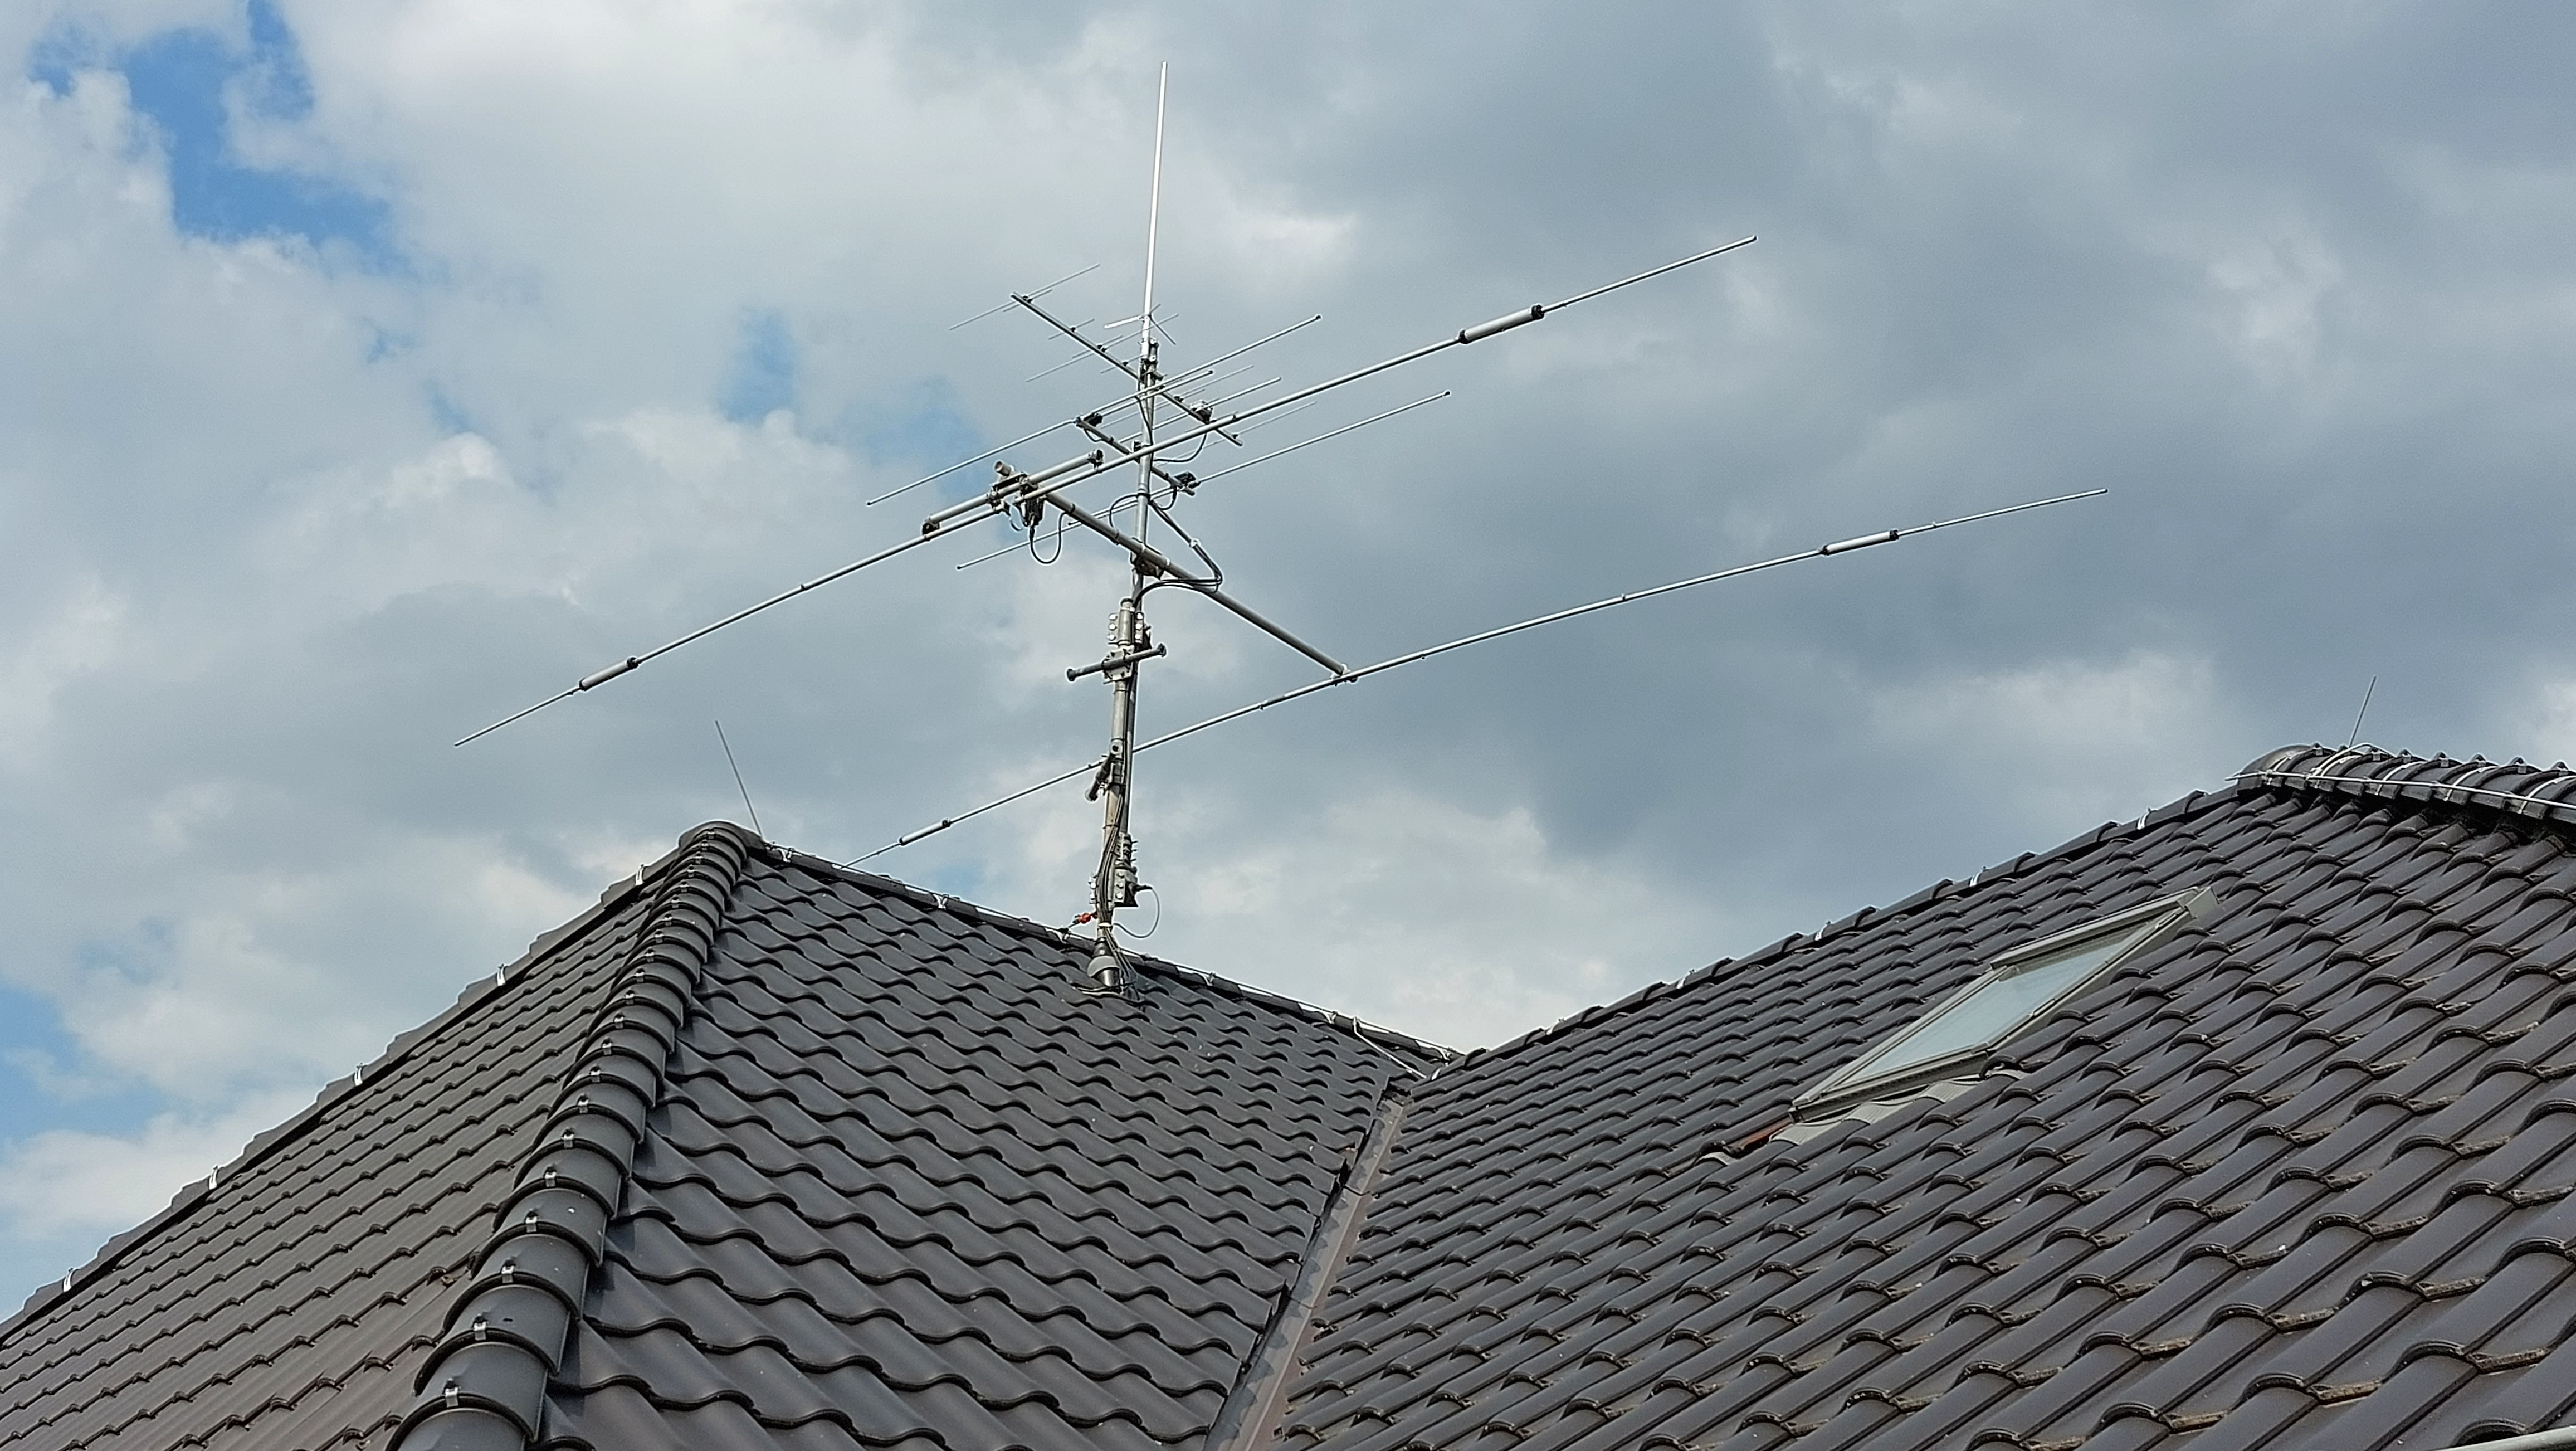
\includegraphics[width=0.85\textwidth]{foto/83}
    \caption{\scriptsize Antennenanlage für KW, VHF und UHF auf einem Hausdach}
    \label{n_antennen_hausdach}
\end{figure}

    \end{column}
   \begin{column}{0.48\textwidth}
       \begin{itemize}
  \item Baurechtliche Bestimmungen des Bundeslandes
  \item Höhe, Abstände zu Nachbargrundstücken, Windlast, etc.
  \item Es haftet der Eigentümer oder Betreiber der Antennenanlage
  \end{itemize}

   \end{column}
\end{columns}

\end{frame}

\begin{frame}
\only<1>{
\begin{QQuestion}{VE602}{Nach welchen Bauvorschriften müssen Außenantennenanlagen errichtet werden?}{Für private Amateurfunkanlagen sind keine besonderen Vorschriften zu beachten.}
{Es gelten die Bestimmungen des Amateurfunkgesetzes (AFuG).}
{Es sind nur die Empfehlungen der Amateurfunkverbände zu beachten.}
{Es gelten die baurechtlichen Bestimmungen des jeweiligen Bundeslandes.}
\end{QQuestion}

}
\only<2>{
\begin{QQuestion}{VE602}{Nach welchen Bauvorschriften müssen Außenantennenanlagen errichtet werden?}{Für private Amateurfunkanlagen sind keine besonderen Vorschriften zu beachten.}
{Es gelten die Bestimmungen des Amateurfunkgesetzes (AFuG).}
{Es sind nur die Empfehlungen der Amateurfunkverbände zu beachten.}
{\textbf{\textcolor{DARCgreen}{Es gelten die baurechtlichen Bestimmungen des jeweiligen Bundeslandes.}}}
\end{QQuestion}

}
\end{frame}

\begin{frame}
\only<1>{
\begin{QQuestion}{VE707}{Wer haftet für Schäden gegenüber Dritten, die durch die Antennenanlage einer Amateurfunkstelle entstehen können?}{Die Amateurfunkvereinigung, wenn der Betreiber der Amateurfunkstelle Mitglied einer solchen Vereinigung ist}
{Der Eigentümer oder Betreiber der Antennenanlage}
{Die Bundesnetzagentur, da in den monatlichen Beiträgen auch ein Anteil für eine Gruppenversicherung für Antennenanlagen von Funkamateuren enthalten ist.}
{Der Grundstückseigentümer, er hat eine Antennenhaftpflichtversicherung abzuschließen, selbst wenn er nicht Betreiber der Amateurfunkstelle ist.}
\end{QQuestion}

}
\only<2>{
\begin{QQuestion}{VE707}{Wer haftet für Schäden gegenüber Dritten, die durch die Antennenanlage einer Amateurfunkstelle entstehen können?}{Die Amateurfunkvereinigung, wenn der Betreiber der Amateurfunkstelle Mitglied einer solchen Vereinigung ist}
{\textbf{\textcolor{DARCgreen}{Der Eigentümer oder Betreiber der Antennenanlage}}}
{Die Bundesnetzagentur, da in den monatlichen Beiträgen auch ein Anteil für eine Gruppenversicherung für Antennenanlagen von Funkamateuren enthalten ist.}
{Der Grundstückseigentümer, er hat eine Antennenhaftpflichtversicherung abzuschließen, selbst wenn er nicht Betreiber der Amateurfunkstelle ist.}
\end{QQuestion}

}
\end{frame}%ENDCONTENT


\section{Energieleitungen}
\label{section:antennen_energieleitungen}
\begin{frame}%STARTCONTENT

\begin{columns}
    \begin{column}{0.48\textwidth}
    
\begin{figure}
    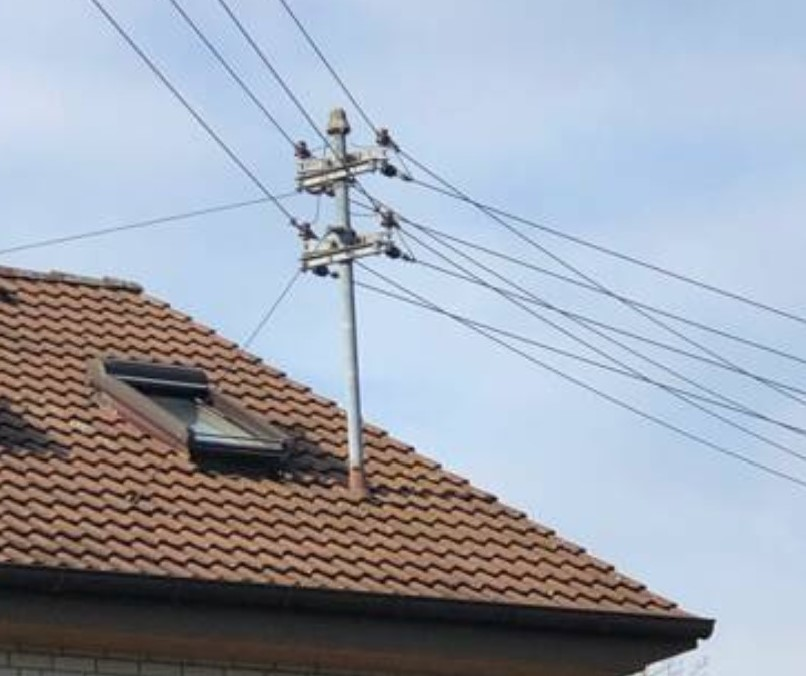
\includegraphics[width=0.85\textwidth]{foto/82}
    \caption{\scriptsize Dachständer}
    \label{n_Dachstaender}
\end{figure}

    \end{column}
   \begin{column}{0.48\textwidth}
       \begin{itemize}
  \item Antenne freihalten von Energieleitungen
  \item Bei Beschädigung der Antenne dürfen keine Teile und Leitungen die Energieversorungsleitungen berühren
  \end{itemize}

   \end{column}
\end{columns}

\end{frame}

\begin{frame}
\frametitle{Achtung}
Wenn eine Antenne eine Energieversorgungsleitung berührt,  besteht akute Gefahr von lebensgefährlichen Stromschlägen!

\end{frame}

\begin{frame}
\only<1>{
\begin{QQuestion}{NK311}{Was ist bei der Installation von Außenantennen insbesondere zu beachten?}{Zu benachbarten Energieversorgungsleitungen ist ein seitlicher Abstand von \qty{8}{\m} einzuhalten.}
{Für die Antenne muss eine Sturmversicherung abgeschlossen werden.}
{An der Antenne müssen die Kontaktdaten des Betreibers erkennbar angebracht sein.}
{Im Falle einer Beschädigung dürfen umstürzende oder herabfallende Teile und Leitungen keine Energieversorgungsleitungen berühren.}
\end{QQuestion}

}
\only<2>{
\begin{QQuestion}{NK311}{Was ist bei der Installation von Außenantennen insbesondere zu beachten?}{Zu benachbarten Energieversorgungsleitungen ist ein seitlicher Abstand von \qty{8}{\m} einzuhalten.}
{Für die Antenne muss eine Sturmversicherung abgeschlossen werden.}
{An der Antenne müssen die Kontaktdaten des Betreibers erkennbar angebracht sein.}
{\textbf{\textcolor{DARCgreen}{Im Falle einer Beschädigung dürfen umstürzende oder herabfallende Teile und Leitungen keine Energieversorgungsleitungen berühren.}}}
\end{QQuestion}

}
\end{frame}%ENDCONTENT


\section{Potentialausgleich}
\label{section:blitzschutz}
\begin{frame}%STARTCONTENT

\frametitle{Potentialausgleich und Erdung}
\begin{itemize}
  \item Durch \emph{Potentialausgleich} wird eine gefährliche Berührungsspannung zwischen den Geräten vermieden
  \item Mittels \emph{Erdung} werden unerwünschte elektrische Ströme vom Gehäuse in die Erde abgeleitet
  \end{itemize}
\end{frame}

\begin{frame}
\begin{columns}
    \begin{column}{0.48\textwidth}
    \begin{itemize}
  \item Geräte mittels kurzer Leitungen zusammenführen
  \item Mit Haupterdungsschiene des Gebäudes verbinden
  \item VDE 0855-300 für Erdung von Funkanlagen
  \end{itemize}

    \end{column}
   \begin{column}{0.48\textwidth}
       
\begin{figure}
    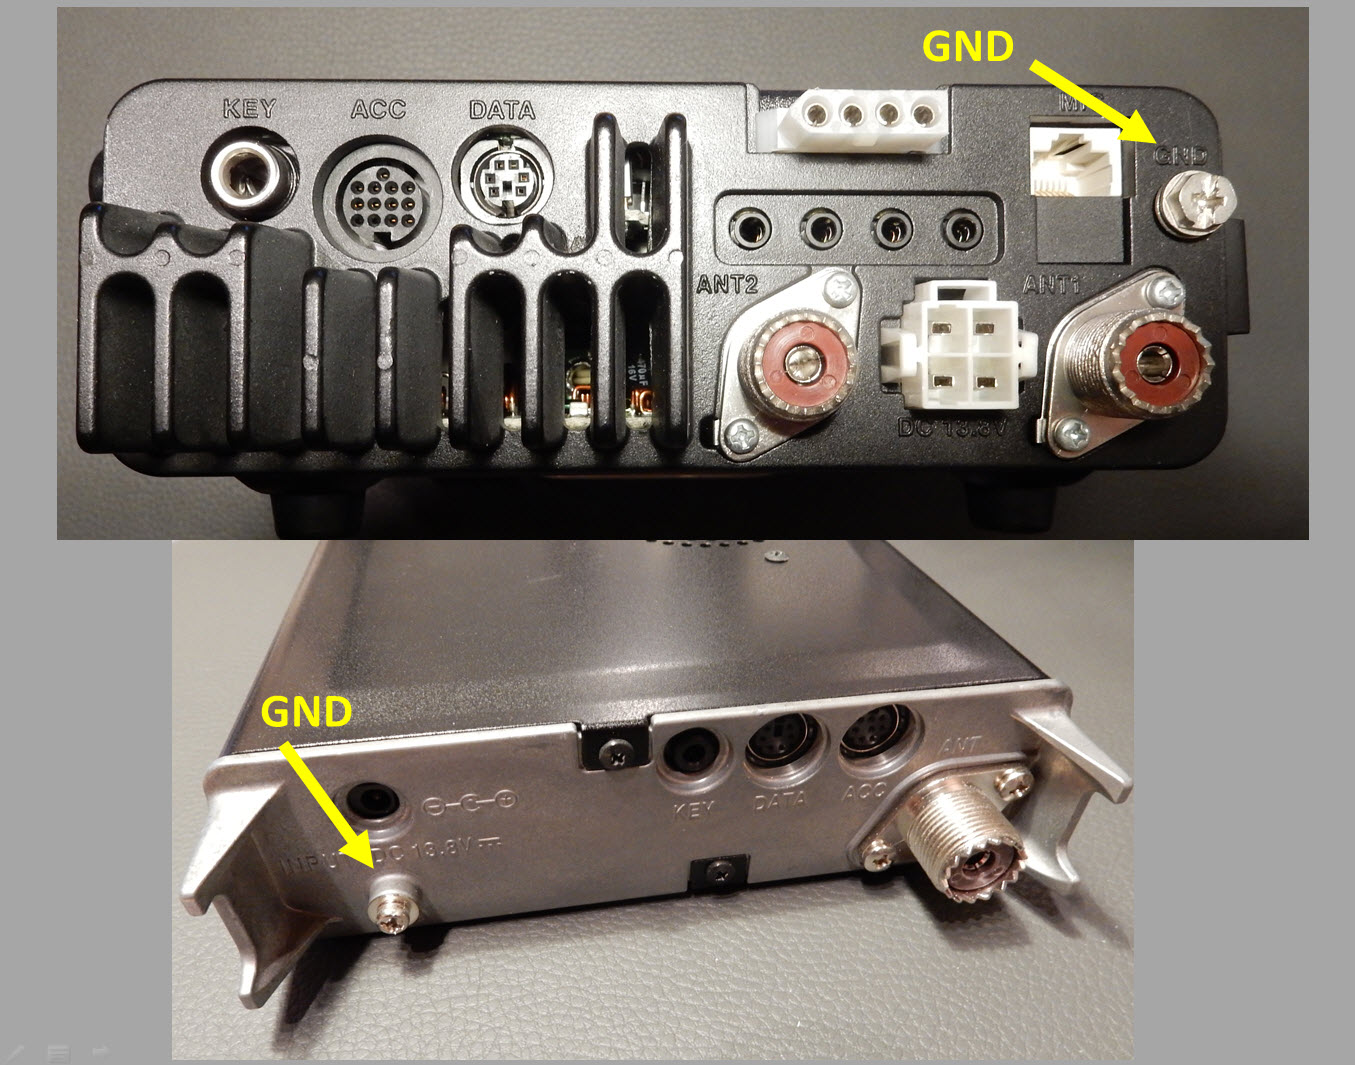
\includegraphics[width=0.85\textwidth]{foto/81}
    \caption{\scriptsize Schraubanschluss Ground (GND) am TRX}
    \label{n_Schraubanschluss_GND}
\end{figure}

   \end{column}
\end{columns}

\end{frame}

\begin{frame}
\frametitle{Achtung}
Der Anschluss von Potentialausgleich und Erdung sollte nur vorgenommen werden, wenn man genau weiß, was man tut. Im Zweifel sollte man sich von einem erfahreneren Funkamateur oder einer Elektrofachkraft helfen lassen.

\end{frame}

\begin{frame}
\only<1>{
\begin{QQuestion}{VE604}{Unter welchen Bedingungen ist die Norm VDE~0855-300 für den Potentialausgleich und die Erdung von Funkanlagen bzw. die Normenreihe VDE~0185-305 zum Blitzschutz heranzuziehen?}{Die Norm VDE~0855-300 gilt für Gebäude, auf denen Antennen errichtet sind. Drahtantennen und freistehende Antennenmasten sind davon ausgenommen.}
{Beide Normen sind dann anzuwenden, wenn Gebäude von Blitzen getroffen werden können.}
{Wenn die Antennenanlage weit genug vom Gebäude entfernt ist, muss die Normreihe VDE~0185-305 nicht angewendet werden.}
{Die Norm VDE~0855-300 gilt für alle Amateurfunk-Sendeanlagen. Die Normenreihe VDE~0185-305 gilt nur für Gebäude mit Blitzschutzsystem.}
\end{QQuestion}

}
\only<2>{
\begin{QQuestion}{VE604}{Unter welchen Bedingungen ist die Norm VDE~0855-300 für den Potentialausgleich und die Erdung von Funkanlagen bzw. die Normenreihe VDE~0185-305 zum Blitzschutz heranzuziehen?}{Die Norm VDE~0855-300 gilt für Gebäude, auf denen Antennen errichtet sind. Drahtantennen und freistehende Antennenmasten sind davon ausgenommen.}
{Beide Normen sind dann anzuwenden, wenn Gebäude von Blitzen getroffen werden können.}
{Wenn die Antennenanlage weit genug vom Gebäude entfernt ist, muss die Normreihe VDE~0185-305 nicht angewendet werden.}
{\textbf{\textcolor{DARCgreen}{Die Norm VDE~0855-300 gilt für alle Amateurfunk-Sendeanlagen. Die Normenreihe VDE~0185-305 gilt nur für Gebäude mit Blitzschutzsystem.}}}
\end{QQuestion}

}
\end{frame}%ENDCONTENT


\title{DARC Amateurfunklehrgang Klasse N}
\author{Transceiver}
\institute{Deutscher Amateur Radio Club e.\,V.}
\begin{frame}
\maketitle
\end{frame}

\section{Aufbau eines Empfängers}
\label{section:aufbau_empfaenger}
\begin{frame}%STARTCONTENT

\frametitle{1. Antenne}
\begin{columns}
    \begin{column}{0.48\textwidth}
    
\begin{figure}
    \DARCimage{0.85\linewidth}{736include}
    \caption{\scriptsize Blockdiagramm eines einfachen Empfängers}
    \label{aufbau_empfaenger_blockdiagramm}
\end{figure}


    \end{column}
   \begin{column}{0.48\textwidth}
       \begin{itemize}
  \item Nimmt Vielzahl von Funkwellen auf
  \item Leitet sie als elektrische Schwingungen weiter
  \end{itemize}

   \end{column}
\end{columns}

\end{frame}

\begin{frame}
\frametitle{2. Bandpassfilter}
\begin{columns}
    \begin{column}{0.48\textwidth}
    
\begin{figure}
    \DARCimage{0.85\linewidth}{736include}
    \caption{\scriptsize Blockdiagramm eines einfachen Empfängers}
    \label{aufbau_empfaenger_blockdiagramm}
\end{figure}


    \end{column}
   \begin{column}{0.48\textwidth}
       \begin{itemize}
  \item Lässt nur gewünschten Frequenzbereich durch
  \item Sperrt alle anderen ungewünschten Frequenzen
  \end{itemize}

   \end{column}
\end{columns}

\end{frame}

\begin{frame}
\frametitle{3. HF-Verstärker}
\begin{columns}
    \begin{column}{0.48\textwidth}
    
\begin{figure}
    \DARCimage{0.85\linewidth}{736include}
    \caption{\scriptsize Blockdiagramm eines einfachen Empfängers}
    \label{aufbau_empfaenger_blockdiagramm}
\end{figure}


    \end{column}
   \begin{column}{0.48\textwidth}
       \begin{itemize}
  \item Verstärkt das herausgefilterte Signal
  \end{itemize}

   \end{column}
\end{columns}

\end{frame}

\begin{frame}
\frametitle{4. Demodulator}
\begin{columns}
    \begin{column}{0.48\textwidth}
    
\begin{figure}
    \DARCimage{0.85\linewidth}{736include}
    \caption{\scriptsize Blockdiagramm eines einfachen Empfängers}
    \label{aufbau_empfaenger_blockdiagramm}
\end{figure}


    \end{column}
   \begin{column}{0.48\textwidth}
       \begin{itemize}
  \item Zurückgewinnung des ursprünglichen Signals, z.B. Sprachsignal
  \item Ergebnis ist das Niederfrequenz-Signal (NF)
  \end{itemize}

   \end{column}
\end{columns}

\end{frame}

\begin{frame}
\frametitle{5. NF-Verstärker}
\begin{columns}
    \begin{column}{0.48\textwidth}
    
\begin{figure}
    \DARCimage{0.85\linewidth}{736include}
    \caption{\scriptsize Blockdiagramm eines einfachen Empfängers}
    \label{aufbau_empfaenger_blockdiagramm}
\end{figure}


    \end{column}
   \begin{column}{0.48\textwidth}
       \begin{itemize}
  \item Verstärkt das demodulierte Signal
  \item NF-Verstärker zum Verstärken des Signals für den Lautsprecher
  \end{itemize}

   \end{column}
\end{columns}

\end{frame}

\begin{frame}
\frametitle{6. Lautsprecher}
\begin{columns}
    \begin{column}{0.48\textwidth}
    
\begin{figure}
    \DARCimage{0.85\linewidth}{736include}
    \caption{\scriptsize Blockdiagramm eines einfachen Empfängers}
    \label{aufbau_empfaenger_blockdiagramm}
\end{figure}


    \end{column}
   \begin{column}{0.48\textwidth}
       \begin{itemize}
  \item Wandelt elektrische Schwingung in Schallwelle um
  \item Signal wird wieder hörbar gemacht
  \end{itemize}

   \end{column}
\end{columns}

\end{frame}

\begin{frame}
\only<1>{
\begin{PQuestion}{NF201}{Was stellt folgendes Blockdiagramm dar?}{Sender}
{Tongenerator}
{Relaisfunkstelle}
{Empfänger}
{\DARCimage{1.0\linewidth}{525include}}\end{PQuestion}

}
\only<2>{
\begin{PQuestion}{NF201}{Was stellt folgendes Blockdiagramm dar?}{Sender}
{Tongenerator}
{Relaisfunkstelle}
{\textbf{\textcolor{DARCgreen}{Empfänger}}}
{\DARCimage{1.0\linewidth}{525include}}\end{PQuestion}

}
\end{frame}

\begin{frame}
\frametitle{Empfindlichkeit}
\begin{itemize}
  \item Je nach Aufbau haben Empfänger unterschiedliche Eigenschaften
  \item Wichtige Eigenschaft: \emph{Empfindlichkeit}
  \item Fähigkeit, schwache Signale zu empfangen
  \item Je empfindlicher, umso schwächere Signale können empfangen werden
  \end{itemize}
\end{frame}

\begin{frame}
\only<1>{
\begin{QQuestion}{NF303}{Worauf bezieht sich die Empfindlichkeit eines Empfängers?}{Auf die Fähigkeit, schwache Signale zu empfangen}
{Auf die Stabilität des VFO}
{Auf die Bandbreite des HF-Vorverstärkers}
{Auf die Fähigkeit, starke Signale zu unterdrücken}
\end{QQuestion}

}
\only<2>{
\begin{QQuestion}{NF303}{Worauf bezieht sich die Empfindlichkeit eines Empfängers?}{\textbf{\textcolor{DARCgreen}{Auf die Fähigkeit, schwache Signale zu empfangen}}}
{Auf die Stabilität des VFO}
{Auf die Bandbreite des HF-Vorverstärkers}
{Auf die Fähigkeit, starke Signale zu unterdrücken}
\end{QQuestion}

}
\end{frame}%ENDCONTENT


\section{RIT}
\label{section:rit}
\begin{frame}%STARTCONTENT
\begin{itemize}
  \item Hört sich in SSB die Gegenstation zu hoch oder tief an $\rightarrow$ \emph{Empfangsfrequenz} korrigieren
  \item Dazu den Regler \emph{RIT} (Receiver Incremental Tuning) verwenden
  \item Beim Verstellen der \emph{Sendefrequenz} versteht mich die Gegenstation schlecht
  \item Ändern beide Stationen jedes Mal die Sendefrequenz entsteht \enquote{über das Band wandern}
  \end{itemize}

\end{frame}

\begin{frame}
\only<1>{
\begin{QQuestion}{NF111}{Die Gegenstation antwortet Ihrem Anruf in SSB-Sprechfunk auf einer geringfügig abweichenden Frequenz. Was sollten Sie tun, um die Empfangsfrequenz Ihres Transceivers anzupassen, ohne dabei die Sendefrequenz zu verstellen?}{Passband-Tuning verstellen}
{Notchfilter einschalten}
{RIT-Einstellung ändern}
{PTT betätigen}
\end{QQuestion}

}
\only<2>{
\begin{QQuestion}{NF111}{Die Gegenstation antwortet Ihrem Anruf in SSB-Sprechfunk auf einer geringfügig abweichenden Frequenz. Was sollten Sie tun, um die Empfangsfrequenz Ihres Transceivers anzupassen, ohne dabei die Sendefrequenz zu verstellen?}{Passband-Tuning verstellen}
{Notchfilter einschalten}
{\textbf{\textcolor{DARCgreen}{RIT-Einstellung ändern}}}
{PTT betätigen}
\end{QQuestion}

}
\end{frame}

\begin{frame}
\frametitle{RIT bei AM und FM}
\begin{itemize}
  \item Nicht notwendig
  \item Verfügen über einen Träger, der zur Demodulation verwendet wird
  \end{itemize}
\end{frame}

\begin{frame}
\only<1>{
\begin{QQuestion}{NF112}{Ihr QSO-Partner meldet bei einem SSB-QSO im \qty{2}{\m}-Band: \glqq Sie senden nicht exakt auf meiner Frequenz\grqq{}. Was könnte die Ursache sein?}{CW-Filter ist aktiviert.}
{LSB ist eingestellt.}
{USB ist eingestellt.}
{RIT ist aktiviert.}
\end{QQuestion}

}
\only<2>{
\begin{QQuestion}{NF112}{Ihr QSO-Partner meldet bei einem SSB-QSO im \qty{2}{\m}-Band: \glqq Sie senden nicht exakt auf meiner Frequenz\grqq{}. Was könnte die Ursache sein?}{CW-Filter ist aktiviert.}
{LSB ist eingestellt.}
{USB ist eingestellt.}
{\textbf{\textcolor{DARCgreen}{RIT ist aktiviert.}}}
\end{QQuestion}

}
\end{frame}%ENDCONTENT


\section{VOX}
\label{section:vox}
\begin{frame}%STARTCONTENT
\begin{itemize}
  \item Automatischer Sendebetrieb durch Spracherkennung statt PTT
  \item \emph{voice-operated exchange} (\emph{VOX})
  \item Beim Sprechen schaltet Transceiver auf Sendung
  \item Bei Stille endet der Sendebetrieb nach kurzer Verzögerung
  \end{itemize}

\end{frame}

\begin{frame}
\only<1>{
\begin{QQuestion}{NF109}{Wie wird die Einstellung bezeichnet, bei der man einen Transceiver durch die Stimme auf Sendung schalten kann?}{SSB}
{PTT}
{RIT}
{VOX}
\end{QQuestion}

}
\only<2>{
\begin{QQuestion}{NF109}{Wie wird die Einstellung bezeichnet, bei der man einen Transceiver durch die Stimme auf Sendung schalten kann?}{SSB}
{PTT}
{RIT}
{\textbf{\textcolor{DARCgreen}{VOX}}}
\end{QQuestion}

}
\end{frame}

\begin{frame}
\only<1>{
\begin{QQuestion}{NF110}{Ihr Transceiver schaltet automatisch auf Sendung. Was kann die Ursache sein?}{VOX ist aktiviert.}
{Squelch ist aktiviert.}
{PTT ist unterbrochen.}
{Relaisablage ist aktiviert.}
\end{QQuestion}

}
\only<2>{
\begin{QQuestion}{NF110}{Ihr Transceiver schaltet automatisch auf Sendung. Was kann die Ursache sein?}{\textbf{\textcolor{DARCgreen}{VOX ist aktiviert.}}}
{Squelch ist aktiviert.}
{PTT ist unterbrochen.}
{Relaisablage ist aktiviert.}
\end{QQuestion}

}
\end{frame}%ENDCONTENT


\section{Squelch}
\label{section:squelch}
\begin{frame}%STARTCONTENT

\begin{columns}
    \begin{column}{0.48\textwidth}
    \begin{itemize}
  \item Auf einer \enquote{leeren} Frequenz hört man Rauschen
  \item Bei FM ist das Rauschen besonders laut
  \item Mit der \emph{Rauschsperre} kann das Rauschen ausgeblendet werden
  \item Englisch \emph{Squelch} (SQL)
  \end{itemize}

    \end{column}
   \begin{column}{0.48\textwidth}
       
\begin{figure}
    \DARCimage{0.85\linewidth}{737include}
    \caption{\scriptsize Zeitlicher Verlauf der Amplitude auf einer Frequenz, zu sehen ist eine starke und eine schwache Sendung, drumherum keine Sendung (Rauschen), der Squelch blendet sowohl Rauschen als auch schwache Signale aus, wenn die Amplitude unter dem eingestellten Wert liegt.}
    \label{squelch}
\end{figure}


   \end{column}
\end{columns}

\end{frame}

\begin{frame}
\only<1>{
\begin{QQuestion}{NF302}{Was muss am Empfänger eingestellt werden, um bei FM das Grundrauschen auszublenden, wenn kein Nutzsignal empfangen wird?}{VOX}
{Squelch}
{RIT}
{Notchfilter}
\end{QQuestion}

}
\only<2>{
\begin{QQuestion}{NF302}{Was muss am Empfänger eingestellt werden, um bei FM das Grundrauschen auszublenden, wenn kein Nutzsignal empfangen wird?}{VOX}
{\textbf{\textcolor{DARCgreen}{Squelch}}}
{RIT}
{Notchfilter}
\end{QQuestion}

}
\end{frame}%ENDCONTENT


\section{Aufbau eines Senders}
\label{section:aufbau_sender}
\begin{frame}%STARTCONTENT

\frametitle{1. Mikrofon}
\begin{columns}
    \begin{column}{0.48\textwidth}
    
\begin{figure}
    \DARCimage{0.85\linewidth}{735include}
    \caption{\scriptsize Blockdiagramm eines einfachen Senders}
    \label{aufbau_sender}
\end{figure}


    \end{column}
   \begin{column}{0.48\textwidth}
       \begin{itemize}
  \item Wandelt Schallwellen in NF-Signal um
  \end{itemize}

   \end{column}
\end{columns}

\end{frame}

\begin{frame}
\frametitle{2. Niederfrequenz-Verstärker}
\begin{columns}
    \begin{column}{0.48\textwidth}
    
\begin{figure}
    \DARCimage{0.85\linewidth}{735include}
    \caption{\scriptsize Blockdiagramm eines einfachen Senders}
    \label{aufbau_sender}
\end{figure}


    \end{column}
   \begin{column}{0.48\textwidth}
       \begin{itemize}
  \item Verstärkt das NF-Signal vom Mikrofon
  \end{itemize}

   \end{column}
\end{columns}

\end{frame}

\begin{frame}
\frametitle{3. Mischer}
\begin{columns}
    \begin{column}{0.48\textwidth}
    
\begin{figure}
    \DARCimage{0.85\linewidth}{735include}
    \caption{\scriptsize Blockdiagramm eines einfachen Senders}
    \label{aufbau_sender}
\end{figure}


    \end{column}
   \begin{column}{0.48\textwidth}
       \begin{itemize}
  \item Mischt das NF-Signal mit dem HF-Träger vom Oszillator (4)
  \end{itemize}

   \end{column}
\end{columns}

\end{frame}

\begin{frame}
\frametitle{4. Oszillator}
\begin{columns}
    \begin{column}{0.48\textwidth}
    
\begin{figure}
    \DARCimage{0.85\linewidth}{735include}
    \caption{\scriptsize Blockdiagramm eines einfachen Senders}
    \label{aufbau_sender}
\end{figure}


    \end{column}
   \begin{column}{0.48\textwidth}
       \begin{itemize}
  \item Erzeugt hochfrequente Schwingung der Sendefrequenz
  \end{itemize}

   \end{column}
\end{columns}

\end{frame}

\begin{frame}
\frametitle{5. Bandfilter}
\begin{columns}
    \begin{column}{0.48\textwidth}
    
\begin{figure}
    \DARCimage{0.85\linewidth}{735include}
    \caption{\scriptsize Blockdiagramm eines einfachen Senders}
    \label{aufbau_sender}
\end{figure}


    \end{column}
   \begin{column}{0.48\textwidth}
       \begin{itemize}
  \item Mischer erzeugt unerwünschte Frequenzen
  \item Mit dem Bandfilter werden nur die gewünschten Frequenzen durchgelassen
  \end{itemize}

   \end{column}
\end{columns}

\end{frame}

\begin{frame}
\frametitle{6. Verstärker}
\begin{columns}
    \begin{column}{0.48\textwidth}
    
\begin{figure}
    \DARCimage{0.85\linewidth}{735include}
    \caption{\scriptsize Blockdiagramm eines einfachen Senders}
    \label{aufbau_sender}
\end{figure}


    \end{column}
   \begin{column}{0.48\textwidth}
       \begin{itemize}
  \item Verstärkt das HF-Signal auf gewünschte Sendeleistung
  \end{itemize}

   \end{column}
\end{columns}

\end{frame}

\begin{frame}
\frametitle{7. Bandfilter}
\begin{columns}
    \begin{column}{0.48\textwidth}
    
\begin{figure}
    \DARCimage{0.85\linewidth}{735include}
    \caption{\scriptsize Blockdiagramm eines einfachen Senders}
    \label{aufbau_sender}
\end{figure}


    \end{column}
   \begin{column}{0.48\textwidth}
       \begin{itemize}
  \item Verstärker kann unerwünschte Frequenzen erzeugen
  \item Nur die gewünschten Frequenzen werden durchgelassen
  \end{itemize}

   \end{column}
\end{columns}

\end{frame}

\begin{frame}
\frametitle{8. Antenne}
\begin{columns}
    \begin{column}{0.48\textwidth}
    
\begin{figure}
    \DARCimage{0.85\linewidth}{735include}
    \caption{\scriptsize Blockdiagramm eines einfachen Senders}
    \label{aufbau_sender}
\end{figure}


    \end{column}
   \begin{column}{0.48\textwidth}
       \begin{itemize}
  \item HF-Signal wird auf Antenne gegeben
  \item Antenne strahlt es als Funkwelle ab
  \end{itemize}

   \end{column}
\end{columns}

\end{frame}

\begin{frame}
\only<1>{
\begin{PQuestion}{NF401}{Was stellt folgendes Blockdiagramm dar?}{Sender}
{Empfänger}
{Relaisfunkstelle}
{Antennenvorverstärker}
{\DARCimage{1.0\linewidth}{524include}}\end{PQuestion}

}
\only<2>{
\begin{PQuestion}{NF401}{Was stellt folgendes Blockdiagramm dar?}{\textbf{\textcolor{DARCgreen}{Sender}}}
{Empfänger}
{Relaisfunkstelle}
{Antennenvorverstärker}
{\DARCimage{1.0\linewidth}{524include}}\end{PQuestion}

}
\end{frame}

\begin{frame}
\only<1>{
\begin{PQuestion}{NF403}{Das nachfolgende Blockschaltbild zeigt einen einfachen Sender. An welcher Stelle befindet sich welche Stufe?}{1 HF-Verstärker; 
2 Filter; 
3 HF-Oszillator;  
4 NF-Verstärker; 
5 Mischer;
6 NF-Verstärker
}
{1 HF-Verstärker; 
2 Mischer; 
3 HF-Oszillator;  
4 Filter; 
5 NF-Verstärker; 
6 Filter
}
{1 NF-Verstärker; 
2 Filter; 
3 HF-Oszillator;  
4 Mischer; 
5 HF-Verstärker;
6 Mischer}
{1 NF-Verstärker; 
2 Mischer; 
3 HF-Oszillator;  
4 Filter; 
5 HF-Verstärker; 
6 Filter}
{\DARCimage{1.0\linewidth}{495include}}\end{PQuestion}

}
\only<2>{
\begin{PQuestion}{NF403}{Das nachfolgende Blockschaltbild zeigt einen einfachen Sender. An welcher Stelle befindet sich welche Stufe?}{1 HF-Verstärker; 
2 Filter; 
3 HF-Oszillator;  
4 NF-Verstärker; 
5 Mischer;
6 NF-Verstärker
}
{1 HF-Verstärker; 
2 Mischer; 
3 HF-Oszillator;  
4 Filter; 
5 NF-Verstärker; 
6 Filter
}
{1 NF-Verstärker; 
2 Filter; 
3 HF-Oszillator;  
4 Mischer; 
5 HF-Verstärker;
6 Mischer}
{\textbf{\textcolor{DARCgreen}{1 NF-Verstärker; 
2 Mischer; 
3 HF-Oszillator;  
4 Filter; 
5 HF-Verstärker; 
6 Filter}}}
{\DARCimage{1.0\linewidth}{495include}}\end{PQuestion}

}
\end{frame}

\begin{frame}
\only<1>{
\begin{QQuestion}{NF402}{Aus welchen Stufen besteht ein einfacher Sender?}{Vorverstärker, Filter, NF-Verstärker, Antenne}
{Vorverstärker, Filter, Demodulator, NF-Verstärker}
{Oszillator, Mischer, Filter, Leistungsverstärker}
{NF-Verstärker, Filter, Leistungsverstärker, Antenne}
\end{QQuestion}

}
\only<2>{
\begin{QQuestion}{NF402}{Aus welchen Stufen besteht ein einfacher Sender?}{Vorverstärker, Filter, NF-Verstärker, Antenne}
{Vorverstärker, Filter, Demodulator, NF-Verstärker}
{\textbf{\textcolor{DARCgreen}{Oszillator, Mischer, Filter, Leistungsverstärker}}}
{NF-Verstärker, Filter, Leistungsverstärker, Antenne}
\end{QQuestion}

}
\end{frame}

\begin{frame}Eine Amateurfunkanlage muss nach den allgemein anerkannten Regeln der Technik aufgebaut und betrieben werden. Das gilt natürlich auch ganz besonders für Sender.

\end{frame}

\begin{frame}
\only<1>{
\begin{QQuestion}{VD106}{Welche technischen Anforderungen stellt die Amateurfunkverordnung u.~a. an eine Amateurfunkstelle?}{Alle für den Sendebetrieb notwendigen Geräte müssen über ein CE-Zeichen verfügen.}
{Sie ist nach den allgemein anerkannten Regeln der Technik einzurichten und zu unterhalten.}
{Das Sendesignal muss über ein Koaxialkabel der Antenne zugeführt werden.}
{Sie darf bauartbedingt keine höhere Leistung erzeugen, als der Besitzer verwenden darf.}
\end{QQuestion}

}
\only<2>{
\begin{QQuestion}{VD106}{Welche technischen Anforderungen stellt die Amateurfunkverordnung u.~a. an eine Amateurfunkstelle?}{Alle für den Sendebetrieb notwendigen Geräte müssen über ein CE-Zeichen verfügen.}
{\textbf{\textcolor{DARCgreen}{Sie ist nach den allgemein anerkannten Regeln der Technik einzurichten und zu unterhalten.}}}
{Das Sendesignal muss über ein Koaxialkabel der Antenne zugeführt werden.}
{Sie darf bauartbedingt keine höhere Leistung erzeugen, als der Besitzer verwenden darf.}
\end{QQuestion}

}
\end{frame}%ENDCONTENT


\section{Ausgangsleistung}
\label{section:ausgangsleistung}
\begin{frame}%STARTCONTENT

\begin{columns}
    \begin{column}{0.48\textwidth}
    \begin{itemize}
  \item Klasse~N ist in Strahlungsleistung (ERP oder EIRP) an Antenne begrenzt
  \end{itemize}

    \end{column}
   \begin{column}{0.48\textwidth}
       \begin{itemize}
  \item Klassen E und A meistens auf \emph{Senderausgangsleistung} (peak envelope power, PEP)
  \end{itemize}

   \end{column}
\end{columns}
    \pause
    \begin{itemize}
  \item Viele Funkgeräte zeigen die aktuelle Senderausgangsleistung im Power-Meter an.
  \end{itemize}


\end{frame}

\begin{frame}
\only<1>{
\begin{PQuestion}{NF102}{Die Darstellung zeigt das Display eines Transceivers. Wie wird die Anzeige 2 im Sendebetrieb bezeichnet?}{Power-Meter}
{Amplitudenspektrum}
{SWR-Meter}
{Wasserfalldiagramm}
{\DARCimage{1.0\linewidth}{578include}}\end{PQuestion}

}
\only<2>{
\begin{PQuestion}{NF102}{Die Darstellung zeigt das Display eines Transceivers. Wie wird die Anzeige 2 im Sendebetrieb bezeichnet?}{\textbf{\textcolor{DARCgreen}{Power-Meter}}}
{Amplitudenspektrum}
{SWR-Meter}
{Wasserfalldiagramm}
{\DARCimage{1.0\linewidth}{578include}}\end{PQuestion}

}
\end{frame}

\begin{frame}
\frametitle{Zulässige Senderausgangsleistung}
\begin{itemize}
  \item In Anlage 1 der AFuV
  \item Unterscheidet sich je nach Klasse und Frequenzbereich
  \end{itemize}

\end{frame}

\begin{frame}
\begin{figure}
    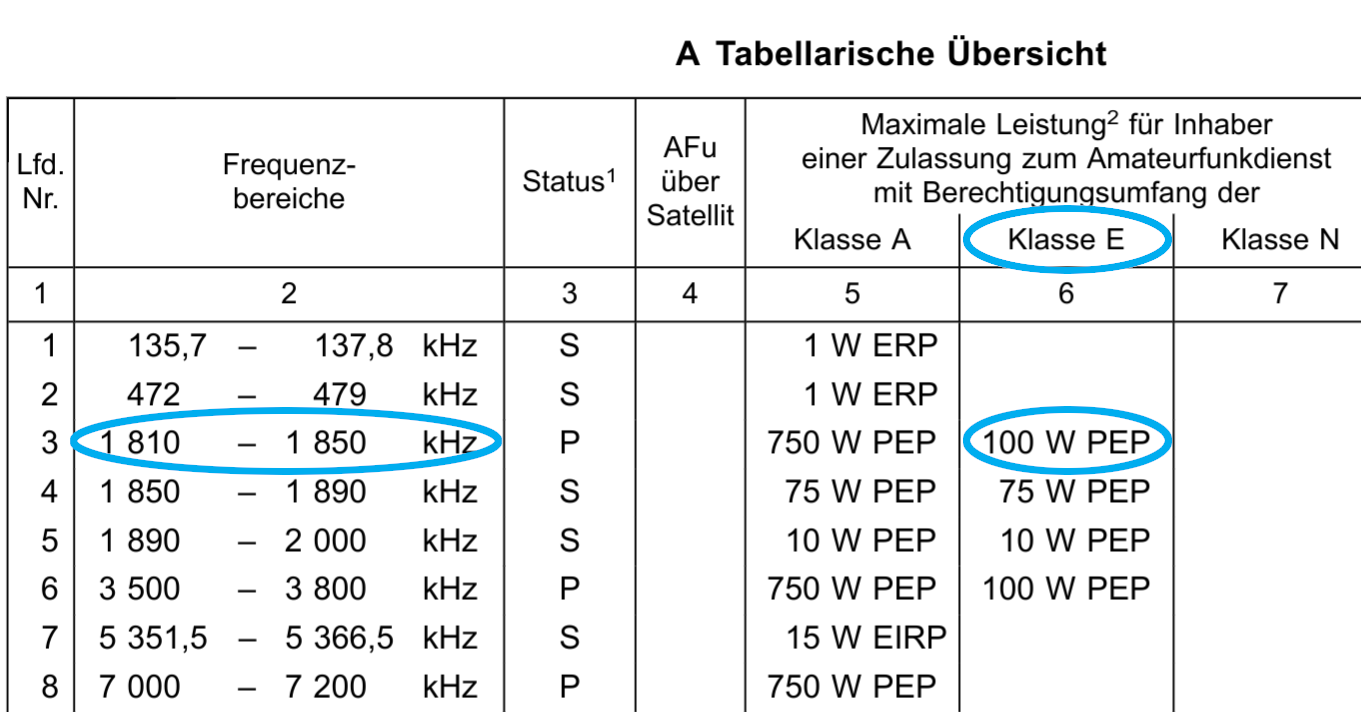
\includegraphics[width=0.85\textwidth]{foto/145}
    \caption{\scriptsize Ausschnitt aus der Anlage 1 der Amateurfunkverordnung}
    \label{ausgangsleistung}
\end{figure}
\end{frame}

\begin{frame}Aktuell ist die Anlage 1 der AFuV (\textcolor{DARCblue}{\faLink~\href{https://50ohm.de/a1}{50ohm.de/a1}}) hier zu finden.

\end{frame}

\begin{frame}
\only<1>{
\begin{QQuestion}{VD727}{Was gilt für die Rufzeicheninhaber der Klasse~E im Frequenzbereich \qtyrange{1810}{1850}{\kHz}?}{Maximal \qty{750}{\W}~PEP}
{Maximal \qty{75}{\W}~PEP }
{Maximal \qty{100}{\W}~PEP}
{Maximal \qty{10}{\W}~PEP}
\end{QQuestion}

}
\only<2>{
\begin{QQuestion}{VD727}{Was gilt für die Rufzeicheninhaber der Klasse~E im Frequenzbereich \qtyrange{1810}{1850}{\kHz}?}{Maximal \qty{750}{\W}~PEP}
{Maximal \qty{75}{\W}~PEP }
{\textbf{\textcolor{DARCgreen}{Maximal \qty{100}{\W}~PEP}}}
{Maximal \qty{10}{\W}~PEP}
\end{QQuestion}

}
\end{frame}

\begin{frame}
\only<1>{
\begin{QQuestion}{VD729}{Was gilt für die Rufzeicheninhaber der Klassen~A~und~E im Frequenzbereich \qtyrange{3,5}{3,8}{\MHz}?}{Maximal \qty{150}{\W}~PEP für Klasse~A und maximal \qty{10}{\W}~PEP für Klasse~E}
{Maximal \qty{10}{\W}~PEP für beide Klassen}
{Maximal \qty{750}{\W}~PEP für beide Klassen}
{Maximal \qty{750}{\W}~PEP für Klasse~A und maximal \qty{100}{\W}~PEP für Klasse~E}
\end{QQuestion}

}
\only<2>{
\begin{QQuestion}{VD729}{Was gilt für die Rufzeicheninhaber der Klassen~A~und~E im Frequenzbereich \qtyrange{3,5}{3,8}{\MHz}?}{Maximal \qty{150}{\W}~PEP für Klasse~A und maximal \qty{10}{\W}~PEP für Klasse~E}
{Maximal \qty{10}{\W}~PEP für beide Klassen}
{Maximal \qty{750}{\W}~PEP für beide Klassen}
{\textbf{\textcolor{DARCgreen}{Maximal \qty{750}{\W}~PEP für Klasse~A und maximal \qty{100}{\W}~PEP für Klasse~E}}}
\end{QQuestion}

}
\end{frame}

\begin{frame}
\only<1>{
\begin{QQuestion}{VD728}{Wie hoch ist die maximal zulässige Senderausgangsleistung für Rufzeicheninhaber der Klasse~A im Frequenzbereich \qtyrange{3,5}{3,8}{\MHz}?}{\qty{75}{\W}~PEP}
{\qty{750}{\W}~PEP}
{\qty{150}{\W}~PEP}
{\qty{100}{\W}~PEP}
\end{QQuestion}

}
\only<2>{
\begin{QQuestion}{VD728}{Wie hoch ist die maximal zulässige Senderausgangsleistung für Rufzeicheninhaber der Klasse~A im Frequenzbereich \qtyrange{3,5}{3,8}{\MHz}?}{\qty{75}{\W}~PEP}
{\textbf{\textcolor{DARCgreen}{\qty{750}{\W}~PEP}}}
{\qty{150}{\W}~PEP}
{\qty{100}{\W}~PEP}
\end{QQuestion}

}
\end{frame}

\begin{frame}
\only<1>{
\begin{QQuestion}{VD730}{Wie hoch ist die maximal zulässige Senderausgangsleistung für Rufzeicheninhaber der Klasse~A im Frequenzbereich \qtyrange{10,1}{10,15}{\MHz}?}{\qty{75}{\W}~PEP}
{\qty{150}{\W}~PEP}
{\qty{250}{\W}~PEP}
{\qty{750}{\W}~PEP}
\end{QQuestion}

}
\only<2>{
\begin{QQuestion}{VD730}{Wie hoch ist die maximal zulässige Senderausgangsleistung für Rufzeicheninhaber der Klasse~A im Frequenzbereich \qtyrange{10,1}{10,15}{\MHz}?}{\qty{75}{\W}~PEP}
{\textbf{\textcolor{DARCgreen}{\qty{150}{\W}~PEP}}}
{\qty{250}{\W}~PEP}
{\qty{750}{\W}~PEP}
\end{QQuestion}

}
\end{frame}

\begin{frame}
\only<1>{
\begin{QQuestion}{VD731}{Wie hoch ist die maximal zulässige Senderausgangsleistung für Rufzeicheninhaber der Klasse~A in den Frequenzbereichen \qtyrange{14,000}{14,350}{\MHz} und \qtyrange{18,068}{18,168}{\MHz}?}{\qty{150}{\W}~PEP}
{\qty{75}{\W}~PEP}
{\qty{750}{\W}~PEP}
{\qty{250}{\W}~PEP}
\end{QQuestion}

}
\only<2>{
\begin{QQuestion}{VD731}{Wie hoch ist die maximal zulässige Senderausgangsleistung für Rufzeicheninhaber der Klasse~A in den Frequenzbereichen \qtyrange{14,000}{14,350}{\MHz} und \qtyrange{18,068}{18,168}{\MHz}?}{\qty{150}{\W}~PEP}
{\qty{75}{\W}~PEP}
{\textbf{\textcolor{DARCgreen}{\qty{750}{\W}~PEP}}}
{\qty{250}{\W}~PEP}
\end{QQuestion}

}
\end{frame}

\begin{frame}
\only<1>{
\begin{QQuestion}{VD732}{Wie hoch ist die maximal zulässige Senderausgangsleistung für Rufzeicheninhaber der Klasse~A in den Frequenzbereichen \qtyrange{21,000}{21,450}{\MHz} und \qtyrange{24,890}{24,990}{\MHz}?}{\qty{150}{\W}~PEP}
{\qty{75}{\W}~PEP}
{\qty{750}{\W}~PEP}
{\qty{250}{\W}~PEP}
\end{QQuestion}

}
\only<2>{
\begin{QQuestion}{VD732}{Wie hoch ist die maximal zulässige Senderausgangsleistung für Rufzeicheninhaber der Klasse~A in den Frequenzbereichen \qtyrange{21,000}{21,450}{\MHz} und \qtyrange{24,890}{24,990}{\MHz}?}{\qty{150}{\W}~PEP}
{\qty{75}{\W}~PEP}
{\textbf{\textcolor{DARCgreen}{\qty{750}{\W}~PEP}}}
{\qty{250}{\W}~PEP}
\end{QQuestion}

}
\end{frame}

\begin{frame}
\only<1>{
\begin{QQuestion}{VD733}{Welche Leistungsgrenzen gelten für die Rufzeicheninhaber der Klassen~A~und~E in den Frequenzbereichen \qtyrange{21,000}{21,450}{\MHz} und \qtyrange{28,000}{29,700}{\MHz}?}{Maximal \qty{100}{\W}~PEP für Klasse~A und maximal \qty{10}{\W}~PEP für Klasse~E}
{Maximal \qty{200}{\W}~PEP für beide Klassen}
{Maximal \qty{750}{\W}~PEP für Klasse~A und maximal \qty{100}{\W}~PEP für Klasse~E}
{Maximal \qty{100}{\W}~PEP für beide Klassen}
\end{QQuestion}

}
\only<2>{
\begin{QQuestion}{VD733}{Welche Leistungsgrenzen gelten für die Rufzeicheninhaber der Klassen~A~und~E in den Frequenzbereichen \qtyrange{21,000}{21,450}{\MHz} und \qtyrange{28,000}{29,700}{\MHz}?}{Maximal \qty{100}{\W}~PEP für Klasse~A und maximal \qty{10}{\W}~PEP für Klasse~E}
{Maximal \qty{200}{\W}~PEP für beide Klassen}
{\textbf{\textcolor{DARCgreen}{Maximal \qty{750}{\W}~PEP für Klasse~A und maximal \qty{100}{\W}~PEP für Klasse~E}}}
{Maximal \qty{100}{\W}~PEP für beide Klassen}
\end{QQuestion}

}
\end{frame}

\begin{frame}
\only<1>{
\begin{QQuestion}{VD734}{Welche Leistungsgrenzen gelten für die Rufzeicheninhaber der Klasse~A~und~E in den Frequenzbereichen \qtyrange{144}{146}{\MHz} und \qtyrange{430}{440}{\MHz}?}{Maximal \qty{750}{\W}~PEP für beide Klassen}
{Maximal \qty{750}{\W}~PEP für Klasse~A und \qty{75}{\W}~PEP für Klasse~E}
{Maximal \qty{100}{\W}~PEP für Klasse~A und \qty{50}{\W}~PEP für Klasse~E}
{Maximal \qty{10}{\W}~PEP für beide Klassen}
\end{QQuestion}

}
\only<2>{
\begin{QQuestion}{VD734}{Welche Leistungsgrenzen gelten für die Rufzeicheninhaber der Klasse~A~und~E in den Frequenzbereichen \qtyrange{144}{146}{\MHz} und \qtyrange{430}{440}{\MHz}?}{Maximal \qty{750}{\W}~PEP für beide Klassen}
{\textbf{\textcolor{DARCgreen}{Maximal \qty{750}{\W}~PEP für Klasse~A und \qty{75}{\W}~PEP für Klasse~E}}}
{Maximal \qty{100}{\W}~PEP für Klasse~A und \qty{50}{\W}~PEP für Klasse~E}
{Maximal \qty{10}{\W}~PEP für beide Klassen}
\end{QQuestion}

}
\end{frame}

\begin{frame}
\only<1>{
\begin{QQuestion}{VD736}{Wie hoch ist die maximal zulässige Senderausgangsleistung für Rufzeicheninhaber der Klasse~A in den Amateurfunkbändern zwischen \qty{1300}{\MHz} und \qty{250}{\GHz}?}{\qty{750}{\W}~PEP}
{\qty{100}{\W}~PEP}
{\qty{150}{\W}~PEP}
{\qty{75}{\W}~PEP}
\end{QQuestion}

}
\only<2>{
\begin{QQuestion}{VD736}{Wie hoch ist die maximal zulässige Senderausgangsleistung für Rufzeicheninhaber der Klasse~A in den Amateurfunkbändern zwischen \qty{1300}{\MHz} und \qty{250}{\GHz}?}{\qty{750}{\W}~PEP}
{\qty{100}{\W}~PEP}
{\qty{150}{\W}~PEP}
{\textbf{\textcolor{DARCgreen}{\qty{75}{\W}~PEP}}}
\end{QQuestion}

}
\end{frame}

\begin{frame}
\only<1>{
\begin{QQuestion}{VD737}{Wie hoch ist die maximal zulässige Senderausgangsleistung für Rufzeicheninhaber der
Klasse E in den Amateurfunkbändern zwischen \qty{1300}{\MHz} und \qty{250}{\GHz}?}{Maximal \qty{75}{\W}~PEP}
{Maximal \qty{5}{\W}~PEP }
{Maximal \qty{100}{\W}~PEP}
{Maximal \qty{1}{\W}~PEP}
\end{QQuestion}

}
\only<2>{
\begin{QQuestion}{VD737}{Wie hoch ist die maximal zulässige Senderausgangsleistung für Rufzeicheninhaber der
Klasse E in den Amateurfunkbändern zwischen \qty{1300}{\MHz} und \qty{250}{\GHz}?}{Maximal \qty{75}{\W}~PEP}
{\textbf{\textcolor{DARCgreen}{Maximal \qty{5}{\W}~PEP }}}
{Maximal \qty{100}{\W}~PEP}
{Maximal \qty{1}{\W}~PEP}
\end{QQuestion}

}
\end{frame}

\begin{frame}\begin{itemize}
  \item Für den Frequenzbereich von \qtyrange{1240}{1300}{\mega\hertz} gelten zusätzliche Regelungen
  \item stehen nicht direkt in der Tabelle
  \item In der rechten Spalte \enquote{Zusätzliche Nutzungsbestimmungen gemäß B} kennzeichnen Zahlen ergänzende Angaben
  \item Stehen unter der Tabelle
  \item Für die folgende Frage ist der Punkt 11 zu beachten
  \end{itemize}
\end{frame}

\begin{frame}
\only<1>{
\begin{QQuestion}{VD735}{Wie hoch ist die maximal zulässige Sendeleistung für Rufzeicheninhaber der Klasse~A im Frequenzbereich \qtyrange{1240}{1300}{\MHz}?}{\qty{250}{\W}~PEP}
{\qty{100}{\W}~PEP}
{\qty{750}{\W}~PEP, jedoch nur maximal \qty{5}{\W}~EIRP im Teilbereich \qtyrange{1247}{1263}{\MHz}}
{\qty{75}{\W}~PEP, jedoch nur maximal \qty{5}{\W}~EIRP im Teilbereich \qtyrange{1247}{1263}{\MHz}}
\end{QQuestion}

}
\only<2>{
\begin{QQuestion}{VD735}{Wie hoch ist die maximal zulässige Sendeleistung für Rufzeicheninhaber der Klasse~A im Frequenzbereich \qtyrange{1240}{1300}{\MHz}?}{\qty{250}{\W}~PEP}
{\qty{100}{\W}~PEP}
{\textbf{\textcolor{DARCgreen}{\qty{750}{\W}~PEP, jedoch nur maximal \qty{5}{\W}~EIRP im Teilbereich \qtyrange{1247}{1263}{\MHz}}}}
{\qty{75}{\W}~PEP, jedoch nur maximal \qty{5}{\W}~EIRP im Teilbereich \qtyrange{1247}{1263}{\MHz}}
\end{QQuestion}

}
\end{frame}%ENDCONTENT


\section{Dummy-Load}
\label{section:dummy_load_1}
\begin{frame}%STARTCONTENT

\begin{columns}
    \begin{column}{0.48\textwidth}
    \begin{itemize}
  \item \emph{Dummy Load} wird für Abgleicharbeiten und Messungen an Sendern verwendet
  \item Ist ein Lastwiderstand
  \item Sendeleistung wird fast vollständig in Wärme umgesetzt
  \item auch: \emph{Abschlusswiderstand} oder \emph{künstliche Antenne}
  \end{itemize}

    \end{column}
   \begin{column}{0.48\textwidth}
       
\begin{figure}
    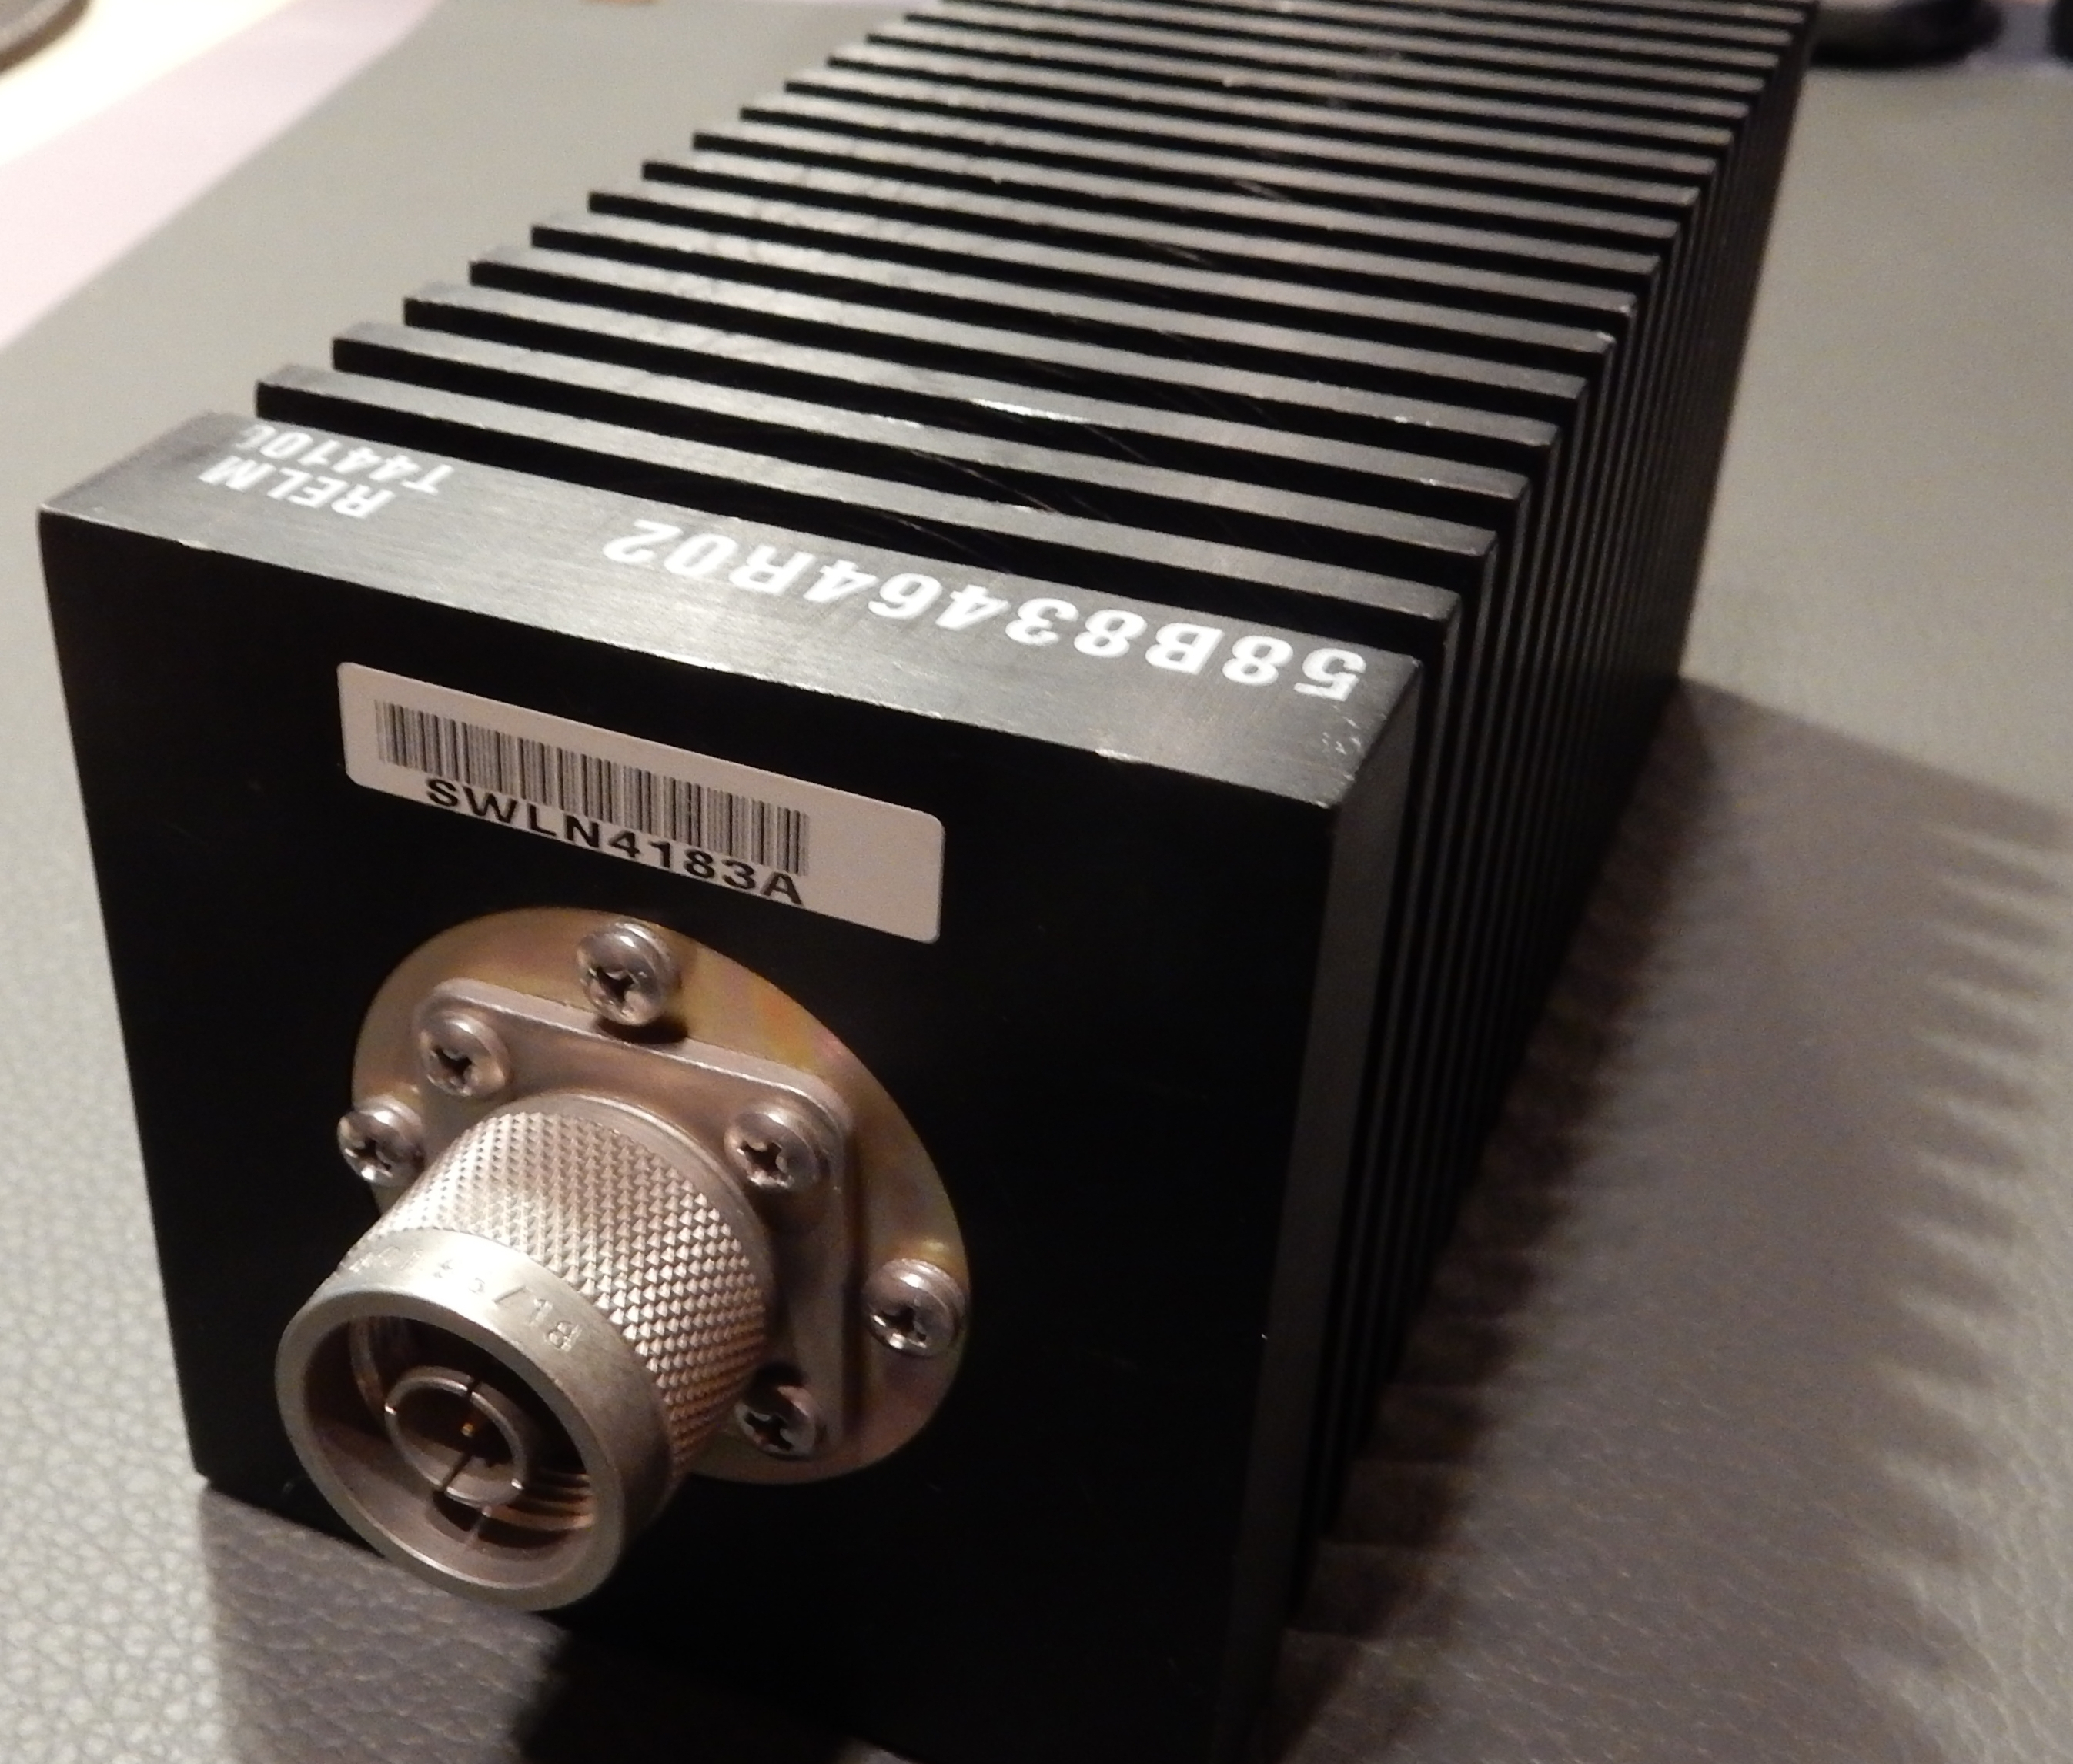
\includegraphics[width=0.85\textwidth]{foto/68}
    \caption{\scriptsize Dummy Load}
    \label{n_antennenanpassung_dummy_load}
\end{figure}

   \end{column}
\end{columns}

\end{frame}

\begin{frame}
\frametitle{Abgleicharbeiten und Messungen}
\begin{itemize}
  \item Immer an möglichst angepasster Antenne oder Dummy Load
  \item Ansonsten kann die Reflektion der Leistung die Endstufe zerstören
  \end{itemize}
\end{frame}

\begin{frame}
\only<1>{
\begin{QQuestion}{VD111}{Was ist bei Abgleicharbeiten und Messungen an Sendern im Hinblick auf die Aussendung zu beachten?}{Das Antennenkabel muss fest angeschlossen sein.}
{Das Sendergehäuse darf nicht geöffnet werden.}
{Es sind geeignete Maßnahmen zu treffen, die ein freies Abstrahlen von Signalen wirkungsvoll verhindern.}
{Es darf nur mit halber Sendeleistung gesendet werden.}
\end{QQuestion}

}
\only<2>{
\begin{QQuestion}{VD111}{Was ist bei Abgleicharbeiten und Messungen an Sendern im Hinblick auf die Aussendung zu beachten?}{Das Antennenkabel muss fest angeschlossen sein.}
{Das Sendergehäuse darf nicht geöffnet werden.}
{\textbf{\textcolor{DARCgreen}{Es sind geeignete Maßnahmen zu treffen, die ein freies Abstrahlen von Signalen wirkungsvoll verhindern.}}}
{Es darf nur mit halber Sendeleistung gesendet werden.}
\end{QQuestion}

}
\end{frame}

\begin{frame}
\only<1>{
\begin{QQuestion}{NJ202}{Wie verhindern Sie beim Abgleichen Ihres selbstgebauten Senders Störungen anderer Funkverbindungen?}{Ich sende nur mit halber Sendeleistung.}
{Ich führe die Abstimmarbeiten auf einer sogenannten ISM-Frequenz aus.}
{Ich verwende einen geeigneten Abschlusswiderstand (Dummy Load).}
{Ich versuche unnötige Modulation zu vermeiden.}
\end{QQuestion}

}
\only<2>{
\begin{QQuestion}{NJ202}{Wie verhindern Sie beim Abgleichen Ihres selbstgebauten Senders Störungen anderer Funkverbindungen?}{Ich sende nur mit halber Sendeleistung.}
{Ich führe die Abstimmarbeiten auf einer sogenannten ISM-Frequenz aus.}
{\textbf{\textcolor{DARCgreen}{Ich verwende einen geeigneten Abschlusswiderstand (Dummy Load).}}}
{Ich versuche unnötige Modulation zu vermeiden.}
\end{QQuestion}

}
\end{frame}

\begin{frame}
\only<1>{
\begin{QQuestion}{NF107}{Warum sollte ein Sender nie ohne angepasste Antenne oder Dummy Load betrieben werden?}{Durch die reflektierte Welle könnte die Senderendstufe beschädigt werden.}
{Durch die fehlende Last wird die Versorgungsspannung hochgeregelt, was zu Überspannungen führen kann. }
{Durch die absorbierte Leistung kann das Netzteil des Senders überlastet werden.  }
{Das Stehwellenmessgerät könnte beschädigt werden.}
\end{QQuestion}

}
\only<2>{
\begin{QQuestion}{NF107}{Warum sollte ein Sender nie ohne angepasste Antenne oder Dummy Load betrieben werden?}{\textbf{\textcolor{DARCgreen}{Durch die reflektierte Welle könnte die Senderendstufe beschädigt werden.}}}
{Durch die fehlende Last wird die Versorgungsspannung hochgeregelt, was zu Überspannungen führen kann. }
{Durch die absorbierte Leistung kann das Netzteil des Senders überlastet werden.  }
{Das Stehwellenmessgerät könnte beschädigt werden.}
\end{QQuestion}

}
\end{frame}

\begin{frame}
\frametitle{Abstimmen}
\begin{itemize}
  \item Aussendungen zum Abstimmen lassen sich nicht vermeiden
  \item Z.B. bei automatischen Anpassgeräten
  \item So kurz wie möglich
  \item Auf freier Frequenz
  \end{itemize}
\end{frame}

\begin{frame}
\only<1>{
\begin{QQuestion}{VD112}{Unter welcher Bedingung ist das Aussenden eines unmodulierten oder ungetasteten Trägers zulässig?}{Sofern es sich um ein digitales Signal handelt}
{Wenn es kurzzeitig erfolgt, z.~B. zum Abstimmen}
{Wenn die Übertragungsbedingungen keine weitreichenden Verbindungen zulassen}
{Sofern die Sendeleistung auf unter \qty{1}{\W} reduziert wird}
\end{QQuestion}

}
\only<2>{
\begin{QQuestion}{VD112}{Unter welcher Bedingung ist das Aussenden eines unmodulierten oder ungetasteten Trägers zulässig?}{Sofern es sich um ein digitales Signal handelt}
{\textbf{\textcolor{DARCgreen}{Wenn es kurzzeitig erfolgt, z.~B. zum Abstimmen}}}
{Wenn die Übertragungsbedingungen keine weitreichenden Verbindungen zulassen}
{Sofern die Sendeleistung auf unter \qty{1}{\W} reduziert wird}
\end{QQuestion}

}
\end{frame}%ENDCONTENT


\section{Unerwünschte Aussendungen}
\label{section:unerwuenschte_aussendungen_1}
\begin{frame}%STARTCONTENT
\begin{itemize}
  \item Amateurfunkverordnung (AFuV): \emph{Unerwünschte Aussendungen} auf das geringstmögliche Maß beschränken
  \item Es gibt weitere gesetzliche Regelungen für konkrete Grenzwerte $\rightarrow$ Klasse~A
  \end{itemize}

\end{frame}

\begin{frame}
\only<1>{
\begin{QQuestion}{NJ201}{Ein Sender sollte so betrieben werden, dass~...}{er keine unerwünschten Aussendungen hervorruft.}
{die Selbsterregung maximiert wird.}
{parasitäre Schwingungen vorhanden sind.}
{die Oberwellenabschirmung minimiert wird.}
\end{QQuestion}

}
\only<2>{
\begin{QQuestion}{NJ201}{Ein Sender sollte so betrieben werden, dass~...}{\textbf{\textcolor{DARCgreen}{er keine unerwünschten Aussendungen hervorruft.}}}
{die Selbsterregung maximiert wird.}
{parasitäre Schwingungen vorhanden sind.}
{die Oberwellenabschirmung minimiert wird.}
\end{QQuestion}

}
\end{frame}

\begin{frame}
\only<1>{
\begin{QQuestion}{NF404}{Welche Eigenschaft sollte ein hinter einem VHF-Sender geschaltetes Filter haben? Dieses sollte...}{den gewünschten Frequenzbereich durchlassen.}
{alle Oberschwingungen durchlassen.}
{die Abstrahlung aller Nebenaussendungen zulassen.}
{den gewünschten Frequenzbereich sperren.}
\end{QQuestion}

}
\only<2>{
\begin{QQuestion}{NF404}{Welche Eigenschaft sollte ein hinter einem VHF-Sender geschaltetes Filter haben? Dieses sollte...}{\textbf{\textcolor{DARCgreen}{den gewünschten Frequenzbereich durchlassen.}}}
{alle Oberschwingungen durchlassen.}
{die Abstrahlung aller Nebenaussendungen zulassen.}
{den gewünschten Frequenzbereich sperren.}
\end{QQuestion}

}
\end{frame}

\begin{frame}
\only<1>{
\begin{QQuestion}{VD110}{Welche Aussage trifft die Amateurfunkverordnung (AFuV) hinsichtlich unerwünschter Aussendungen?}{Unerwünschte Aussendungen sind auf \qty{60}{\decibel} bezogen auf das Nutzsignal zu beschränken.}
{Unerwünschte Aussendungen sind auf das geringstmögliche Maß zu beschränken.}
{Unerwünschte Aussendungen sind auf \qty{40}{\decibel} bezogen auf das Nutzsignal zu beschränken.}
{Unerwünschte Aussendungen sind nicht zulässig.}
\end{QQuestion}

}
\only<2>{
\begin{QQuestion}{VD110}{Welche Aussage trifft die Amateurfunkverordnung (AFuV) hinsichtlich unerwünschter Aussendungen?}{Unerwünschte Aussendungen sind auf \qty{60}{\decibel} bezogen auf das Nutzsignal zu beschränken.}
{\textbf{\textcolor{DARCgreen}{Unerwünschte Aussendungen sind auf das geringstmögliche Maß zu beschränken.}}}
{Unerwünschte Aussendungen sind auf \qty{40}{\decibel} bezogen auf das Nutzsignal zu beschränken.}
{Unerwünschte Aussendungen sind nicht zulässig.}
\end{QQuestion}

}
\end{frame}%ENDCONTENT


\section{Elektromagnetische Verträglichkeit}
\label{section:elektromagnetische_vertraeglichkeit}
\begin{frame}%STARTCONTENT

\frametitle{Beim Senden}
    \pause
    
\begin{columns}
    \begin{column}{0.48\textwidth}
    Funkwellen von

\begin{itemize}
  \item von Antennen
  \item von Transceivern
  \item von Zuleitungen
  \end{itemize}

    \end{column}
    \pause
    
   \begin{column}{0.48\textwidth}
       Elektrische Schwingungen gelangen in andere Leitungen

\begin{itemize}
  \item Zerstörungen von anderen elektronischen Geräten
  \item Geräusche aus Lautsprechern
  \item Internetausfall
  \item Fehler in Heizungssteuerung
  \end{itemize}

   \end{column}
\end{columns}



\end{frame}

\begin{frame}
\frametitle{Beim Senden}
Einhalten der Schutzanforderungen zur Gewährleistung der elektromagnetischen Verträglichkeit im Sinne des Gesetzes über die elektromagnetische Verträglichkeit von Betriebsmitteln (EMVG)

\end{frame}

\begin{frame}
\only<1>{
\begin{QQuestion}{VC118}{Was muss ein Funkamateur beim Betrieb seiner Amateurfunkstelle in Bezug auf die elektromagnetische Verträglichkeit beachten?}{Die Amateurfunkstelle darf nur aus baumustergeprüften Funkgeräten bestehen, die den Anforderungen des Gesetzes über Funkanlagen (FuAG) entsprechen.}
{Der Funkamateur benötigt für seine Amateurfunkstelle eine aktuelle  Verträglichkeitsbescheinigung der BNetzA.
}
{Der Funkamateur muss die Schutzanforderungen zur Gewährleistung der elektromagnetischen Verträglichkeit im Sinne des Gesetzes über die elektromagnetische Verträglichkeit von Betriebsmitteln (EMVG) einhalten.}
{Die Amateurfunkstelle muss von einem zertifizierten Elektromeister auf die Einhaltung der elektromagnetischen Verträglichkeit geprüft werden. Das Abnahmeprotokoll ist für die BNetzA bereitzuhalten.
}
\end{QQuestion}

}
\only<2>{
\begin{QQuestion}{VC118}{Was muss ein Funkamateur beim Betrieb seiner Amateurfunkstelle in Bezug auf die elektromagnetische Verträglichkeit beachten?}{Die Amateurfunkstelle darf nur aus baumustergeprüften Funkgeräten bestehen, die den Anforderungen des Gesetzes über Funkanlagen (FuAG) entsprechen.}
{Der Funkamateur benötigt für seine Amateurfunkstelle eine aktuelle  Verträglichkeitsbescheinigung der BNetzA.
}
{\textbf{\textcolor{DARCgreen}{Der Funkamateur muss die Schutzanforderungen zur Gewährleistung der elektromagnetischen Verträglichkeit im Sinne des Gesetzes über die elektromagnetische Verträglichkeit von Betriebsmitteln (EMVG) einhalten.}}}
{Die Amateurfunkstelle muss von einem zertifizierten Elektromeister auf die Einhaltung der elektromagnetischen Verträglichkeit geprüft werden. Das Abnahmeprotokoll ist für die BNetzA bereitzuhalten.
}
\end{QQuestion}

}
\end{frame}

\begin{frame}
\frametitle{Beim Empfang}
Funkamateur darf Störfestigkeit der eigenen Geräte selbst bestimmen. Die Abweichung vom EMVG ist ein Privileg.

\end{frame}

\begin{frame}
\only<1>{
\begin{QQuestion}{VC120}{Darf der Funkamateur bei Selbstbaugeräten von den grundlegenden Anforderungen zur Störfestigkeit im Sinne des Gesetzes über die elektromagnetische Verträglichkeit von Betriebsmitteln (EMVG) abweichen?}{Nein, die Störfestigkeit ist vorgegeben und muss eingehalten werden.}
{Ja, aber nur in Richtung Verbesserung der Störfestigkeit}
{Ja, er kann den Grad der Störfestigkeit seiner Geräte selbst bestimmen.}
{Nein, selbstgebaute Amateurfunkgeräte müssen im Bezug auf Störfestigkeit  kommerziell hergestellten Geräten entsprechen.}
\end{QQuestion}

}
\only<2>{
\begin{QQuestion}{VC120}{Darf der Funkamateur bei Selbstbaugeräten von den grundlegenden Anforderungen zur Störfestigkeit im Sinne des Gesetzes über die elektromagnetische Verträglichkeit von Betriebsmitteln (EMVG) abweichen?}{Nein, die Störfestigkeit ist vorgegeben und muss eingehalten werden.}
{Ja, aber nur in Richtung Verbesserung der Störfestigkeit}
{\textbf{\textcolor{DARCgreen}{Ja, er kann den Grad der Störfestigkeit seiner Geräte selbst bestimmen.}}}
{Nein, selbstgebaute Amateurfunkgeräte müssen im Bezug auf Störfestigkeit  kommerziell hergestellten Geräten entsprechen.}
\end{QQuestion}

}
\end{frame}

\begin{frame}
\only<1>{
\begin{QQuestion}{VC119}{Was gilt hinsichtlich der Störfestigkeit der Amateurfunkstelle nach dem Wortlaut des Amateurfunkgesetzes (AFuG)? }{Der Funkamateur darf von den grundlegenden Anforderungen nach dem Gesetz über die elektromagnetische Verträglichkeit von Betriebsmitteln (EMVG) abweichen und kann den Grad der Störfestigkeit seiner Amateurfunkstelle selbst bestimmen.}
{Der Funkamateur muss seine Amateurfunkstelle im Abstand von 2 Jahren einer Störfestigkeitsprüfung durch die BNetzA unterziehen lassen.}
{Amateurfunkstellen sind hinsichtlich ihrer Störfestigkeit anderen Betriebsmitteln gleichgestellt.}
{Amateurfunkstellen müssen elektromagnetische Störungen durch andere Betriebsmittel hinnehmen, selbst wenn diese nicht den grundlegenden Anforderungen nach dem Gesetz über die elektromagnetische Verträglichkeit von Betriebsmitteln (EMVG) entsprechen.}
\end{QQuestion}

}
\only<2>{
\begin{QQuestion}{VC119}{Was gilt hinsichtlich der Störfestigkeit der Amateurfunkstelle nach dem Wortlaut des Amateurfunkgesetzes (AFuG)? }{\textbf{\textcolor{DARCgreen}{Der Funkamateur darf von den grundlegenden Anforderungen nach dem Gesetz über die elektromagnetische Verträglichkeit von Betriebsmitteln (EMVG) abweichen und kann den Grad der Störfestigkeit seiner Amateurfunkstelle selbst bestimmen.}}}
{Der Funkamateur muss seine Amateurfunkstelle im Abstand von 2 Jahren einer Störfestigkeitsprüfung durch die BNetzA unterziehen lassen.}
{Amateurfunkstellen sind hinsichtlich ihrer Störfestigkeit anderen Betriebsmitteln gleichgestellt.}
{Amateurfunkstellen müssen elektromagnetische Störungen durch andere Betriebsmittel hinnehmen, selbst wenn diese nicht den grundlegenden Anforderungen nach dem Gesetz über die elektromagnetische Verträglichkeit von Betriebsmitteln (EMVG) entsprechen.}
\end{QQuestion}

}
\end{frame}

\begin{frame}
\frametitle{Maßnahmen}
Zur Einhaltung der vorgeschriebenen elektromagnetischen Verträglichkeit (EMV)

\begin{itemize}
  \item Abschirmen
  \item Erden
  \end{itemize}
    \pause
    Schutz vor Störungen in beide Richtungen



\end{frame}

\begin{frame}
\only<1>{
\begin{QQuestion}{NK101}{In Bezug auf EMV sollten HF-Stufen~...}{gut abgeschirmt werden.}
{eine besonders abgeschirmte Masseleitung erhalten.}
{in Kunststoff eingehüllt werden.}
{nur kapazitive Auskopplungen enthalten.}
\end{QQuestion}

}
\only<2>{
\begin{QQuestion}{NK101}{In Bezug auf EMV sollten HF-Stufen~...}{\textbf{\textcolor{DARCgreen}{gut abgeschirmt werden.}}}
{eine besonders abgeschirmte Masseleitung erhalten.}
{in Kunststoff eingehüllt werden.}
{nur kapazitive Auskopplungen enthalten.}
\end{QQuestion}

}
\end{frame}

\begin{frame}
\only<1>{
\begin{QQuestion}{NJ101}{Alle Geräte, die HF-Ströme übertragen, sollten~...}{möglichst gut geschirmt sein.}
{nicht geerdet sein.}
{über das Stromversorgungsnetz geerdet sein.}
{durch Kunststoffabdeckungen geschützt sein.}
\end{QQuestion}

}
\only<2>{
\begin{QQuestion}{NJ101}{Alle Geräte, die HF-Ströme übertragen, sollten~...}{\textbf{\textcolor{DARCgreen}{möglichst gut geschirmt sein.}}}
{nicht geerdet sein.}
{über das Stromversorgungsnetz geerdet sein.}
{durch Kunststoffabdeckungen geschützt sein.}
\end{QQuestion}

}
\end{frame}

\begin{frame}
\only<1>{
\begin{QQuestion}{NK102}{Um eine Amateurfunkstelle in Bezug auf EMV zu optimieren,~...}{sollten alle hochohmigen Erdverbindungen entfernt werden.}
{sollte der Sender mit der Wasserleitung im Haus verbunden werden.}
{sollten alle Einrichtungen mit einer guten HF-Erdung versehen werden.}
{sollte der Sender mit der Abwasserleitung im Haus verbunden werden.}
\end{QQuestion}

}
\only<2>{
\begin{QQuestion}{NK102}{Um eine Amateurfunkstelle in Bezug auf EMV zu optimieren,~...}{sollten alle hochohmigen Erdverbindungen entfernt werden.}
{sollte der Sender mit der Wasserleitung im Haus verbunden werden.}
{\textbf{\textcolor{DARCgreen}{sollten alle Einrichtungen mit einer guten HF-Erdung versehen werden.}}}
{sollte der Sender mit der Abwasserleitung im Haus verbunden werden.}
\end{QQuestion}

}
\end{frame}%ENDCONTENT


\section{Störungen vermeiden}
\label{section:stoerungen_vermeiden}
\begin{frame}%STARTCONTENT

\frametitle{Gründe für Störungen}
\begin{itemize}
  \item Unerwünschte Frequenzanteile, die nicht ausreichend unterdrückt werden
  \item Unzureichend abgeschirmte oder unzureichend geerdete Geräte 
  \item Die gewünschten Aussendungen selber
  \end{itemize}
\end{frame}

\begin{frame}
\frametitle{Störung}
\begin{columns}
    \begin{column}{0.48\textwidth}
    
\begin{figure}
    \DARCimage{0.85\linewidth}{745include}
    \caption{\scriptsize Störung des DVB-T2-Empfang eines Fernsehers durch die Oberschwingung einer Amateurfunkaussendung}
    \label{stoerungen_vermeiden_oberschwingung}
\end{figure}


    \end{column}
   \begin{column}{0.48\textwidth}
       \begin{itemize}
  \item Grenzwerte durch Amateurfunkanlage überschritten
  \item Z.B. Oberschwingung
  \end{itemize}

   \end{column}
\end{columns}

\end{frame}

\begin{frame}
\frametitle{Störende Beeinflussung}
\begin{columns}
    \begin{column}{0.48\textwidth}
    
\begin{figure}
    \DARCimage{0.85\linewidth}{744include}
    \caption{\scriptsize Einstrahlung über die Empfangsantenne}
    \label{stoerungen_vermeiden_einstrahlung}
\end{figure}


\begin{figure}
    \DARCimage{0.85\linewidth}{746include}
    \caption{\scriptsize Direkteinstrahlung in ein Gerät}
    \label{stoerungen_vermeiden_direkteinstrahlung}
\end{figure}


    \end{column}
   \begin{column}{0.48\textwidth}
       
\begin{figure}
    \DARCimage{0.85\linewidth}{747include}
    \caption{\scriptsize Einströmung über Anschlussleitungen}
    \label{stoerungen_vermeiden_einstroemung}
\end{figure}

\begin{itemize}
  \item Grenzwerte werden eingehalten
  \item Wege können einzeln oder zusammen auftreten
  \end{itemize}

   \end{column}
\end{columns}

\end{frame}

\begin{frame}
\frametitle{Umgang mit Störungen}
\begin{itemize}
  \item Nachbarschaftskonflikte vermeiden
  \item Höflich Hilfe zur Entstörung anbieten
  \end{itemize}
\end{frame}

\begin{frame}
\only<1>{
\begin{QQuestion}{NJ102}{Welche Reaktion ist angebracht, wenn ihr Nachbar sich über Störungen beklagt?}{Sie bieten höflich an, die erforderlichen Prüfungen in die Wege zu leiten.}
{Er sollte höflich darauf hingewiesen werden, dass es an seiner eigenen Einrichtung liegt.}
{Er sollte darauf hingewiesen werden, dass Sie hierfür nicht zuständig sind.}
{Sie bieten an, das örtlich zuständige Hauptzollamt zu benachrichtigen.}
\end{QQuestion}

}
\only<2>{
\begin{QQuestion}{NJ102}{Welche Reaktion ist angebracht, wenn ihr Nachbar sich über Störungen beklagt?}{\textbf{\textcolor{DARCgreen}{Sie bieten höflich an, die erforderlichen Prüfungen in die Wege zu leiten.}}}
{Er sollte höflich darauf hingewiesen werden, dass es an seiner eigenen Einrichtung liegt.}
{Er sollte darauf hingewiesen werden, dass Sie hierfür nicht zuständig sind.}
{Sie bieten an, das örtlich zuständige Hauptzollamt zu benachrichtigen.}
\end{QQuestion}

}
\end{frame}

\begin{frame}
\frametitle{Ursachenforschung}
\begin{itemize}
  \item Prüfen auf Behebung mit eigenen Mitteln
  \item Falls Ursache nicht ermittelt oder Störung nicht beseitigt werden kann $\rightarrow$ Nachbarn auf \emph{Funkstörungsannahme der BNetzA} (24/7~ aPhone ~0228~14~15~16) hinweisen
  \end{itemize}

\end{frame}

\begin{frame}
\only<1>{
\begin{QQuestion}{VE302}{Welche Reaktion ist angebracht, wenn Störungen im Fernseh- oder Rundfunkempfang beim Nachbarn nicht mit den zur Verfügung stehenden Mitteln beseitigt werden können?}{Sie empfehlen dem Nachbarn höflich, sich an die Bundesnetzagentur zur Prüfung der Störungsursache zu wenden.}
{Der Nachbar sollte höflich darauf hingewiesen werden, dass es an seiner eigenen Einrichtung liegt.}
{Der Nachbar sollte darauf hingewiesen werden, dass Sie hierfür nicht zuständig sind.}
{Sie benachrichtigen ihren Amateurfunkverband.}
\end{QQuestion}

}
\only<2>{
\begin{QQuestion}{VE302}{Welche Reaktion ist angebracht, wenn Störungen im Fernseh- oder Rundfunkempfang beim Nachbarn nicht mit den zur Verfügung stehenden Mitteln beseitigt werden können?}{\textbf{\textcolor{DARCgreen}{Sie empfehlen dem Nachbarn höflich, sich an die Bundesnetzagentur zur Prüfung der Störungsursache zu wenden.}}}
{Der Nachbar sollte höflich darauf hingewiesen werden, dass es an seiner eigenen Einrichtung liegt.}
{Der Nachbar sollte darauf hingewiesen werden, dass Sie hierfür nicht zuständig sind.}
{Sie benachrichtigen ihren Amateurfunkverband.}
\end{QQuestion}

}
\end{frame}

\begin{frame}
\frametitle{Ermittlung}
\begin{itemize}
  \item Kann einige Zeit in Anspruch nehmen
  \item Zur Wahrung des Nachbarschaftsfriedens Sendeleistung reduzieren
  \end{itemize}
\end{frame}

\begin{frame}
\only<1>{
\begin{QQuestion}{VE301}{Durch den Betrieb einer Amateurfunkstelle wird der Rundfunkempfang eines Nachbarn gestört. Welche Maßnahme kann der Funkamateur zur Wahrung des nachbarschaftlichen Friedens noch vor Einschaltung der Bundesnetzagentur durchführen?}{Er kann die Sendeleistung vorläufig reduzieren.}
{Er schaltet am Transceiver Passband-Tuning ein.}
{Er macht ausschließlich DX-Betrieb.}
{Er macht ausschließlich Split-Betrieb. }
\end{QQuestion}

}
\only<2>{
\begin{QQuestion}{VE301}{Durch den Betrieb einer Amateurfunkstelle wird der Rundfunkempfang eines Nachbarn gestört. Welche Maßnahme kann der Funkamateur zur Wahrung des nachbarschaftlichen Friedens noch vor Einschaltung der Bundesnetzagentur durchführen?}{\textbf{\textcolor{DARCgreen}{Er kann die Sendeleistung vorläufig reduzieren.}}}
{Er schaltet am Transceiver Passband-Tuning ein.}
{Er macht ausschließlich DX-Betrieb.}
{Er macht ausschließlich Split-Betrieb. }
\end{QQuestion}

}
\end{frame}

\begin{frame}
\frametitle{Überprüfung}
Falls Amateurfunkaussendungen die Ursache der Probleme sind, wird in drei Fälle unterschieden

\end{frame}

\begin{frame}
\frametitle{1. Fall}
\begin{itemize}
  \item Amateurfunkanlage wird \emph{nicht vorschriftsmäßig} betrieben
  \item Ggf. Anordnung einer kostenpflichtigen Betriebseinschränkung durch BNetzA
  \item Möglich ist eine Begrenzung der Sendeleistung
  \end{itemize}

\end{frame}

\begin{frame}
\frametitle{2. Fall}
\begin{itemize}
  \item Amateurfunkanlage wird \emph{vorschriftsmäßig} betrieben
  \item Feldstärke am betroffenen Gerät ist kleiner als Verträglichkeit durch die Störfestigkeit
  \item Betroffenes Gerät \emph{hält Störfestigkeit nicht ein}
  \item Verantwortung zur Behebung liegt beim Betreiber des betroffenen Geräts
  \item Funkamateur darf Sendebetrieb unverändert fortsetzen
  \end{itemize}
\end{frame}

\begin{frame}
\only<1>{
\begin{QQuestion}{VE305}{Durch den Betrieb einer Amateurfunkstelle auf \qty{145,550}{\MHz} wird der UKW-Rundfunkempfänger eines Nachbarn durch Direkteinstrahlung beeinträchtigt. Eine Überprüfung ergibt, dass der Funkamateur am Ort des beeinträchtigten Empfängers eine Feldstärke erzeugt, die den in der Norm empfohlenen Grenzwert für die Störfestigkeit von Geräten nicht erreicht. Was folgt daraus für den Funkamateur?}{Er kann seinen Funkbetrieb fortsetzen.}
{Er hat seine Sendeleistung so einzurichten, dass der Empfang nicht mehr beeinträchtigt wird.}
{Er kann seine Sendeleistung uneingeschränkt erhöhen.}
{Er hat den Betrieb seiner Amateurfunkstelle einzustellen.}
\end{QQuestion}

}
\only<2>{
\begin{QQuestion}{VE305}{Durch den Betrieb einer Amateurfunkstelle auf \qty{145,550}{\MHz} wird der UKW-Rundfunkempfänger eines Nachbarn durch Direkteinstrahlung beeinträchtigt. Eine Überprüfung ergibt, dass der Funkamateur am Ort des beeinträchtigten Empfängers eine Feldstärke erzeugt, die den in der Norm empfohlenen Grenzwert für die Störfestigkeit von Geräten nicht erreicht. Was folgt daraus für den Funkamateur?}{\textbf{\textcolor{DARCgreen}{Er kann seinen Funkbetrieb fortsetzen.}}}
{Er hat seine Sendeleistung so einzurichten, dass der Empfang nicht mehr beeinträchtigt wird.}
{Er kann seine Sendeleistung uneingeschränkt erhöhen.}
{Er hat den Betrieb seiner Amateurfunkstelle einzustellen.}
\end{QQuestion}

}
\end{frame}

\begin{frame}
\only<1>{
\begin{QQuestion}{VE306}{Durch den Betrieb einer Amateurfunkstelle auf \qty{144,250}{\MHz} wird der Kabelfernsehempfang eines Nachbarn beeinträchtigt. Eine Überprüfung ergibt, dass der Funkamateur am Ort der beeinträchtigten Empfangsanlage eine Feldstärke erzeugt, die den in der Norm empfohlenen Grenzwert für die Störfestigkeit von Kabelverteilanlagen nicht erreicht. Was folgt daraus für den Funkamateur?}{Er kann seinen Funkbetrieb fortsetzen.}
{Er hat den Betrieb seiner Amateurfunkstelle einzustellen.}
{Er hat seine Sendeleistung so einzurichten, dass der Empfang nicht mehr beeinträchtigt wird.}
{Er kann seine Sendeleistung uneingeschränkt erhöhen.}
\end{QQuestion}

}
\only<2>{
\begin{QQuestion}{VE306}{Durch den Betrieb einer Amateurfunkstelle auf \qty{144,250}{\MHz} wird der Kabelfernsehempfang eines Nachbarn beeinträchtigt. Eine Überprüfung ergibt, dass der Funkamateur am Ort der beeinträchtigten Empfangsanlage eine Feldstärke erzeugt, die den in der Norm empfohlenen Grenzwert für die Störfestigkeit von Kabelverteilanlagen nicht erreicht. Was folgt daraus für den Funkamateur?}{\textbf{\textcolor{DARCgreen}{Er kann seinen Funkbetrieb fortsetzen.}}}
{Er hat den Betrieb seiner Amateurfunkstelle einzustellen.}
{Er hat seine Sendeleistung so einzurichten, dass der Empfang nicht mehr beeinträchtigt wird.}
{Er kann seine Sendeleistung uneingeschränkt erhöhen.}
\end{QQuestion}

}
\end{frame}

\begin{frame}
\frametitle{3. Fall}
\begin{itemize}
  \item Amateurfunkanlage wird \emph{vorschriftsmäßig} betrieben
  \item Betroffenes Gerät \emph{hält Storfestigkeit ein}
  \item Konfliktfall: BNetzA ist befugt, eine Lösung \emph{in Zusammenarbeit mit allen Beteilgten} herzustellen
  \end{itemize}
\end{frame}

\begin{frame}
\only<1>{
\begin{QQuestion}{VE303}{Durch den Betrieb einer Amateurfunkstelle auf \qty{145,550}{\MHz} wird der UKW-Rundfunkempfang eines Nachbarn beeinträchtigt. Eine Überprüfung ergibt, dass sowohl die Amateurfunkstelle als auch die Rundfunkempfangsanlage vorschriftsmäßig betrieben werden. Womit muss der Funkamateur rechnen?}{Mit einer gebührenpflichtigen Betriebseinschränkung oder einem vollständigen Betriebsverbot für seine Amateurfunkstelle}
{Mit behördlichen Abhilfemaßnahmen in Zusammenarbeit mit den Beteiligten}
{Mit der Durchführung behördlicher Maßnahmen nach dem AFuG, wobei dem Funkamateur die Zulassung zur Teilnahme am Amateurfunkdienst entzogen werden kann}
{Mit einem Ordnungswidrigkeitenverfahren mit Betriebsverbot und Bußgeld auf der Grundlage des AFuG}
\end{QQuestion}

}
\only<2>{
\begin{QQuestion}{VE303}{Durch den Betrieb einer Amateurfunkstelle auf \qty{145,550}{\MHz} wird der UKW-Rundfunkempfang eines Nachbarn beeinträchtigt. Eine Überprüfung ergibt, dass sowohl die Amateurfunkstelle als auch die Rundfunkempfangsanlage vorschriftsmäßig betrieben werden. Womit muss der Funkamateur rechnen?}{Mit einer gebührenpflichtigen Betriebseinschränkung oder einem vollständigen Betriebsverbot für seine Amateurfunkstelle}
{\textbf{\textcolor{DARCgreen}{Mit behördlichen Abhilfemaßnahmen in Zusammenarbeit mit den Beteiligten}}}
{Mit der Durchführung behördlicher Maßnahmen nach dem AFuG, wobei dem Funkamateur die Zulassung zur Teilnahme am Amateurfunkdienst entzogen werden kann}
{Mit einem Ordnungswidrigkeitenverfahren mit Betriebsverbot und Bußgeld auf der Grundlage des AFuG}
\end{QQuestion}

}
\end{frame}

\begin{frame}
\only<1>{
\begin{QQuestion}{VE304}{Durch den Betrieb einer Amateurfunkstelle wird der Fernsehempfang eines Nachbarn beeinträchtigt. Eine Überprüfung ergibt, dass sowohl das Fernsehgerät als auch die Amateurfunkstelle die Vorschriften einhalten und Nachbesserungen nicht mehr möglich sind. Wozu ist die BNetzA in diesem Fall befugt?}{Die BNetzA kann Abhilfemaßnahmen in Zusammenarbeit mit den Beteiligten veranlassen.}
{Die BNetzA hat diesbezüglich keine Befugnisse.}
{Zum sofortigen Widerruf der Zulassung zum Amateurfunkdienst}
{Zur Einleitung eines Bußgeldverfahrens}
\end{QQuestion}

}
\only<2>{
\begin{QQuestion}{VE304}{Durch den Betrieb einer Amateurfunkstelle wird der Fernsehempfang eines Nachbarn beeinträchtigt. Eine Überprüfung ergibt, dass sowohl das Fernsehgerät als auch die Amateurfunkstelle die Vorschriften einhalten und Nachbesserungen nicht mehr möglich sind. Wozu ist die BNetzA in diesem Fall befugt?}{\textbf{\textcolor{DARCgreen}{Die BNetzA kann Abhilfemaßnahmen in Zusammenarbeit mit den Beteiligten veranlassen.}}}
{Die BNetzA hat diesbezüglich keine Befugnisse.}
{Zum sofortigen Widerruf der Zulassung zum Amateurfunkdienst}
{Zur Einleitung eines Bußgeldverfahrens}
\end{QQuestion}

}
\end{frame}

\begin{frame}
\frametitle{Anordnungen der BNetzA ohne Zusammenarbeit}
\begin{itemize}
  \item Zum Schutz von Empfangs- und Sendegeräten, die Sicherheitszwecken dienen
  \item Zum Schutz öffentlicher Telekommunikationsnetze, also beispielsweise dem Telefonnetz
  \item Zum Schutz von Leib und Leben einer Person oder Sachen von bedeutendem Wert
  \end{itemize}

\end{frame}%ENDCONTENT


\section{Störungen beim Empfang}
\label{section:empfangsstoerungen}
\begin{frame}%STARTCONTENT

\frametitle{Suche im eigenen Haushalt}
Häufige Ursachen

\begin{itemize}
  \item Wechselrichter von Solaranlagen
  \item Schaltnetzteile
  \item LED-Leuchten
  \item Powerline Communication
  \end{itemize}

\end{frame}

\begin{frame}
\only<1>{
\begin{QQuestion}{VE307}{Der Empfang Ihrer Amateurfunkstation ist auf allen Bändern gestört. Welche Maßnahme sollten Sie als erstes ergreifen?}{Störquellen im eigenen Haushalt suchen, z. B. Steckernetzteile, LED-Lampen, Computer und Bildschirme.}
{Die Funkstörungsannahme der Bundesnetzagentur telefonisch oder per E-Mail informieren.}
{Das Intruder Monitoring eines Amateurfunkverbandes informieren.}
{Den Empfangsbetrieb sofort einstellen und z. B. auf Sendebetrieb umstellen.}
\end{QQuestion}

}
\only<2>{
\begin{QQuestion}{VE307}{Der Empfang Ihrer Amateurfunkstation ist auf allen Bändern gestört. Welche Maßnahme sollten Sie als erstes ergreifen?}{\textbf{\textcolor{DARCgreen}{Störquellen im eigenen Haushalt suchen, z. B. Steckernetzteile, LED-Lampen, Computer und Bildschirme.}}}
{Die Funkstörungsannahme der Bundesnetzagentur telefonisch oder per E-Mail informieren.}
{Das Intruder Monitoring eines Amateurfunkverbandes informieren.}
{Den Empfangsbetrieb sofort einstellen und z. B. auf Sendebetrieb umstellen.}
\end{QQuestion}

}
\end{frame}

\begin{frame}
\frametitle{Hinnehmbare Störungen}
\begin{itemize}
  \item Versuchen, die Grenzwerte von Geräten in der Nachbarschaft festzustellen
  \item Werden die Grenzwerte (EMVG und FuAG) eingehalten, muss die Störung hingenommen werden
  \item Evtl. hat der Nachbar Kooperationsbereitschaft zur Behebung
  \end{itemize}

\end{frame}

\begin{frame}
\only<1>{
\begin{QQuestion}{VE308}{Muss ein Funkamateur eine Störung seines Empfangs durch andere Geräte hinnehmen?}{Er muss die Störungen grundsätzlich hinnehmen, wenn die störenden Geräte den Anforderungen des Gesetzes über die elektromagnetische Verträglichkeit von Betriebsmitteln (EMVG) oder des Funkanlagengesetzes (FuAG) genügen.}
{Er muss Störungen nicht hinnehmen.}
{Er muss die Störungen in jedem Fall hinnehmen.}
{Er muss die Störungen grundsätzlich hinnehmen, wenn das störende Gerät von erheblicher Bedeutung für den Betreiber ist (z.~B. von einer Alarmanlage).}
\end{QQuestion}

}
\only<2>{
\begin{QQuestion}{VE308}{Muss ein Funkamateur eine Störung seines Empfangs durch andere Geräte hinnehmen?}{\textbf{\textcolor{DARCgreen}{Er muss die Störungen grundsätzlich hinnehmen, wenn die störenden Geräte den Anforderungen des Gesetzes über die elektromagnetische Verträglichkeit von Betriebsmitteln (EMVG) oder des Funkanlagengesetzes (FuAG) genügen.}}}
{Er muss Störungen nicht hinnehmen.}
{Er muss die Störungen in jedem Fall hinnehmen.}
{Er muss die Störungen grundsätzlich hinnehmen, wenn das störende Gerät von erheblicher Bedeutung für den Betreiber ist (z.~B. von einer Alarmanlage).}
\end{QQuestion}

}
\end{frame}

\begin{frame}
\frametitle{BNetzA einbeziehen}
\begin{itemize}
  \item Über Funkstörannahme der Bundesnetzagentur
  \item Protokoll über Störungen erstellen
  \item Zeitpunkt, Art und vermutete Quelle
  \end{itemize}
\end{frame}

\begin{frame}
\only<1>{
\begin{QQuestion}{VE309}{Der Empfang Ihrer Amateurfunkstation ist wiederkehrend gestört. Die Ursache liegt nicht in Ihrem Haushalt. Sie wollen die Funkstörungsannahme der Bundesnetzagentur informieren. Wie sollten Sie die Bearbeitung durch die Behörde unterstützen?}{Ich sammele die Kontaktdaten aller Nachbarn und melde diese per E-Mail.}
{Ich sende bei jedem einzelnen Auftreten der Störung eine E-Mail.}
{Ich dränge auf ein schnelles Ausrücken des Prüf- und Messdienstes und frage regelmäßig telefonisch nach dem Stand.}
{Ich fertige ein Protokoll mit Zeitpunkt und Art der Störungen an und benenne die vermutete Quelle.}
\end{QQuestion}

}
\only<2>{
\begin{QQuestion}{VE309}{Der Empfang Ihrer Amateurfunkstation ist wiederkehrend gestört. Die Ursache liegt nicht in Ihrem Haushalt. Sie wollen die Funkstörungsannahme der Bundesnetzagentur informieren. Wie sollten Sie die Bearbeitung durch die Behörde unterstützen?}{Ich sammele die Kontaktdaten aller Nachbarn und melde diese per E-Mail.}
{Ich sende bei jedem einzelnen Auftreten der Störung eine E-Mail.}
{Ich dränge auf ein schnelles Ausrücken des Prüf- und Messdienstes und frage regelmäßig telefonisch nach dem Stand.}
{\textbf{\textcolor{DARCgreen}{Ich fertige ein Protokoll mit Zeitpunkt und Art der Störungen an und benenne die vermutete Quelle.}}}
\end{QQuestion}

}
\end{frame}%ENDCONTENT


\title{DARC Amateurfunklehrgang Klasse N}
\author{Logbuch und QSL-Karten}
\institute{Deutscher Amateur Radio Club e.\,V.}
\begin{frame}
\maketitle
\end{frame}

\section{Logbuch}
\label{section:logbuch}
\begin{frame}%STARTCONTENT
\begin{itemize}
  \item Mit einem Logbuch hat man die Möglichkeit, seine Funkaktivitäten zu dokumentieren
  \item Die Führung eines Logbuchs ist freiwillig
  \end{itemize}

\end{frame}

\begin{frame}Folgende Daten werden üblicherweise in einem Logbuch für jede Funkverbindung festgehalten:

\begin{itemize}
  \item Rufzeichen der Gegenstation
  \item Frequenz oder Band
  \item Datum und Uhrzeit
  \item Übertragungsverfahren (z.\,B. SSB, FT8, RTTY,~...)
  \item Vergebener und erhaltener Rapport
  \item Verwendete Sendeleistung
  \item Bemerkungen (z.B. Name des QSO-Partners oder eigene verwendete Station)
  \end{itemize}
\end{frame}

\begin{frame}
\only<1>{
\begin{QQuestion}{BG101}{Was verstehen Funkamateure unter einem Logbuch?}{Es ist die Dokumentation aller Geräte und Antennen des Funkamateurs.}
{Es ist das Stationstagebuch, das jeder Funkamateur führen muss.}
{Es ist das Stationstagebuch, das ein Funkamateur freiwillig führt oder in besonderen Fällen führen muss.}
{Es ist die Dokumentation über die Einhaltung der Sicherheitsabstände bezüglich des Personenschutzes.}
\end{QQuestion}

}
\only<2>{
\begin{QQuestion}{BG101}{Was verstehen Funkamateure unter einem Logbuch?}{Es ist die Dokumentation aller Geräte und Antennen des Funkamateurs.}
{Es ist das Stationstagebuch, das jeder Funkamateur führen muss.}
{\textbf{\textcolor{DARCgreen}{Es ist das Stationstagebuch, das ein Funkamateur freiwillig führt oder in besonderen Fällen führen muss.}}}
{Es ist die Dokumentation über die Einhaltung der Sicherheitsabstände bezüglich des Personenschutzes.}
\end{QQuestion}

}
\end{frame}

\begin{frame}
\frametitle{Verpflichtende Logbuchführung}
Es kann aber auch dazu kommen, dass man eine Aufforderung der Bundesnetzagentur erhält, die einen verpflichtet, ein Logbuch zu führen.

\begin{itemize}
  \item Zur Untersuchung von Störungsursachen
  \item Zur Klärung frequenztechnischer Fragen
  \end{itemize}
\end{frame}

\begin{frame}
\only<1>{
\begin{QQuestion}{VD109}{Wann muss der Funkamateur Angaben über den Betrieb seiner Amateurfunkstelle schriftlich festhalten, z. B. als Logbuch?}{Bei Funkbetrieb auf der Kurzwelle}
{Auf Verlangen der Bundesnetzagentur}
{Bei internationalem Funkbetrieb}
{In den ersten 12 Monaten nach der Zulassung}
\end{QQuestion}

}
\only<2>{
\begin{QQuestion}{VD109}{Wann muss der Funkamateur Angaben über den Betrieb seiner Amateurfunkstelle schriftlich festhalten, z. B. als Logbuch?}{Bei Funkbetrieb auf der Kurzwelle}
{\textbf{\textcolor{DARCgreen}{Auf Verlangen der Bundesnetzagentur}}}
{Bei internationalem Funkbetrieb}
{In den ersten 12 Monaten nach der Zulassung}
\end{QQuestion}

}
\end{frame}

\begin{frame}
\only<1>{
\begin{QQuestion}{VD108}{Zu welchen Zwecken kann die Bundesnetzagentur schriftliche Nachweise über den Funkbetrieb verlangen?}{Zur Überprüfung der Qualifikation des Funkamateurs und des Inhalts seiner Aussendungen}
{Zur Untersuchung von Störungsursachen oder zur Klärung frequenztechnischer Fragen}
{Als Nachweis für die Einhaltung von Grenzwerten nach dem Bundes-Immissionsschutzgesetz (BImSchG)}
{Als Nachweis zur Abrechnung der Frequenznutzungsbeiträge}
\end{QQuestion}

}
\only<2>{
\begin{QQuestion}{VD108}{Zu welchen Zwecken kann die Bundesnetzagentur schriftliche Nachweise über den Funkbetrieb verlangen?}{Zur Überprüfung der Qualifikation des Funkamateurs und des Inhalts seiner Aussendungen}
{\textbf{\textcolor{DARCgreen}{Zur Untersuchung von Störungsursachen oder zur Klärung frequenztechnischer Fragen}}}
{Als Nachweis für die Einhaltung von Grenzwerten nach dem Bundes-Immissionsschutzgesetz (BImSchG)}
{Als Nachweis zur Abrechnung der Frequenznutzungsbeiträge}
\end{QQuestion}

}
\end{frame}

\begin{frame}
\frametitle{Aufbewahrung des Logbuchs}
\begin{itemize}
  \item Bei angeordneter Logbuchführung
  \item Über eine bestimmte Zeit einsehbar
  \item Bei elektronischem Logbuch ist Transfer mit ADIF-Dateiformat möglich
  \item Bei Transfer von Papier auf elektronisch muss das Papierformat weiter aufbewahrt werden
  \end{itemize}
\end{frame}

\begin{frame}
\only<1>{
\begin{QQuestion}{BG102}{Was ist bei der Erstellung eines \glqq Computer-Logbuchs\grqq{} bei angeordneter Logbuchführung zu beachten?}{Die Logdatei muss auch mit einem Textverarbeitungsprogramm gelesen werden können.}
{Die Daten müssen, wie auch beim Papierlogbuch, über eine bestimmte Zeit einsehbar sein.}
{Es muss zusätzlich ein herkömmliches Papierlogbuch geführt werden.}
{Es muss jederzeit ein Ausdruck des Logbuches vorhanden sein.}
\end{QQuestion}

}
\only<2>{
\begin{QQuestion}{BG102}{Was ist bei der Erstellung eines \glqq Computer-Logbuchs\grqq{} bei angeordneter Logbuchführung zu beachten?}{Die Logdatei muss auch mit einem Textverarbeitungsprogramm gelesen werden können.}
{\textbf{\textcolor{DARCgreen}{Die Daten müssen, wie auch beim Papierlogbuch, über eine bestimmte Zeit einsehbar sein.}}}
{Es muss zusätzlich ein herkömmliches Papierlogbuch geführt werden.}
{Es muss jederzeit ein Ausdruck des Logbuches vorhanden sein.}
\end{QQuestion}

}
\end{frame}

\begin{frame}
\only<1>{
\begin{QQuestion}{BG103}{Was ist bei angeordneter Logbuchführung bei einem Wechsel der \glqq Logbuchsoftware\grqq{} zu berücksichtigen?}{Es sollte auf eine Software für ein \qty{64}{\bit}-System gewechselt werden.}
{Die Logbuchdaten müssen verfügbar bleiben, um die Betriebsdaten bei eventuellen späteren Überprüfungen einsehen zu können.}
{Die alte Software muss auf jeden Fall gelöscht werden, um Kollisionen bei den Datenformaten zu vermeiden.}
{Es sollte ein Logbuchprogramm genutzt werden, welches ermöglicht, die Daten in der Cloud zu speichern.}
\end{QQuestion}

}
\only<2>{
\begin{QQuestion}{BG103}{Was ist bei angeordneter Logbuchführung bei einem Wechsel der \glqq Logbuchsoftware\grqq{} zu berücksichtigen?}{Es sollte auf eine Software für ein \qty{64}{\bit}-System gewechselt werden.}
{\textbf{\textcolor{DARCgreen}{Die Logbuchdaten müssen verfügbar bleiben, um die Betriebsdaten bei eventuellen späteren Überprüfungen einsehen zu können.}}}
{Die alte Software muss auf jeden Fall gelöscht werden, um Kollisionen bei den Datenformaten zu vermeiden.}
{Es sollte ein Logbuchprogramm genutzt werden, welches ermöglicht, die Daten in der Cloud zu speichern.}
\end{QQuestion}

}
\end{frame}

\begin{frame}
\frametitle{Koordinierte Weltzeit}
\begin{itemize}
  \item Zeiten in UTC (Universal Time Coordinated) führen
  \item Uhrzeiten über unterschiedliche Zeitzonen müssen nicht umgerechnet werden
  \item Keine Probleme mit Sommer-/Winterzeit
  \item Berlin zu Mitteleuropäischer Zeit (MEZ): UTC+1
  \item Berlin zu Mitteleuropäischer Sommerzeit (MESZ): UTC+2
  \end{itemize}
\end{frame}%ENDCONTENT


\section{QSL-Karten}
\label{section:qsl_karten}
\begin{frame}%STARTCONTENT

\begin{columns}
    \begin{column}{0.48\textwidth}
    \begin{itemize}
  \item Nachweis darüber, dass eine Funkverbindung tatsächlich stattgefunden hat
  \item Dienen als Beleg bei der Beantragung von Amateurfunk-Diplomen
  \item Q-Gruppe QSL mit \enquote{ich bestätige den Empfang}
  \end{itemize}

    \end{column}
   \begin{column}{0.48\textwidth}
       
\begin{figure}
    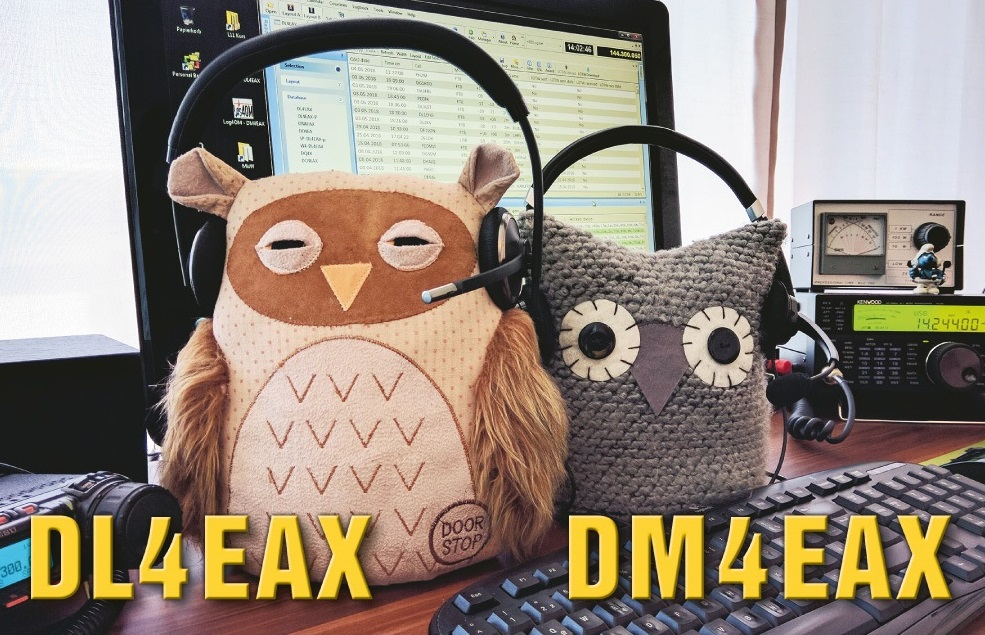
\includegraphics[width=0.85\textwidth]{foto/12}
    \caption{\scriptsize Gemeinsame QSL-Karte von DL4EAX und DM4EAX (Vorderseite)}
    \label{n_qsl_karten_vorderseite}
\end{figure}

   \end{column}
\end{columns}

\end{frame}

\begin{frame}
\only<1>{
\begin{QQuestion}{BG104}{Eine QSL-Karte ist~...}{eine Reservierungsbestätigung für die Teilnahme an einer Amateurfunkrunde. Sie sichert dem Funkamateur einen Listenplatz in der Runde.}
{die Bescheinigung über die Mitgliedschaft in einer Amateurfunkvereinigung.}
{eine Landkarte, in der Standorte für ortsgebundene Funkwettbewerbe eingezeichnet sind.}
{die Bestätigung einer Amateurfunkverbindung. Sie dient z. B. als Beleg bei der Beantragung von Amateurfunk-Diplomen.}
\end{QQuestion}

}
\only<2>{
\begin{QQuestion}{BG104}{Eine QSL-Karte ist~...}{eine Reservierungsbestätigung für die Teilnahme an einer Amateurfunkrunde. Sie sichert dem Funkamateur einen Listenplatz in der Runde.}
{die Bescheinigung über die Mitgliedschaft in einer Amateurfunkvereinigung.}
{eine Landkarte, in der Standorte für ortsgebundene Funkwettbewerbe eingezeichnet sind.}
{\textbf{\textcolor{DARCgreen}{die Bestätigung einer Amateurfunkverbindung. Sie dient z. B. als Beleg bei der Beantragung von Amateurfunk-Diplomen.}}}
\end{QQuestion}

}
\end{frame}

\begin{frame}
\frametitle{Angaben}

\begin{figure}
    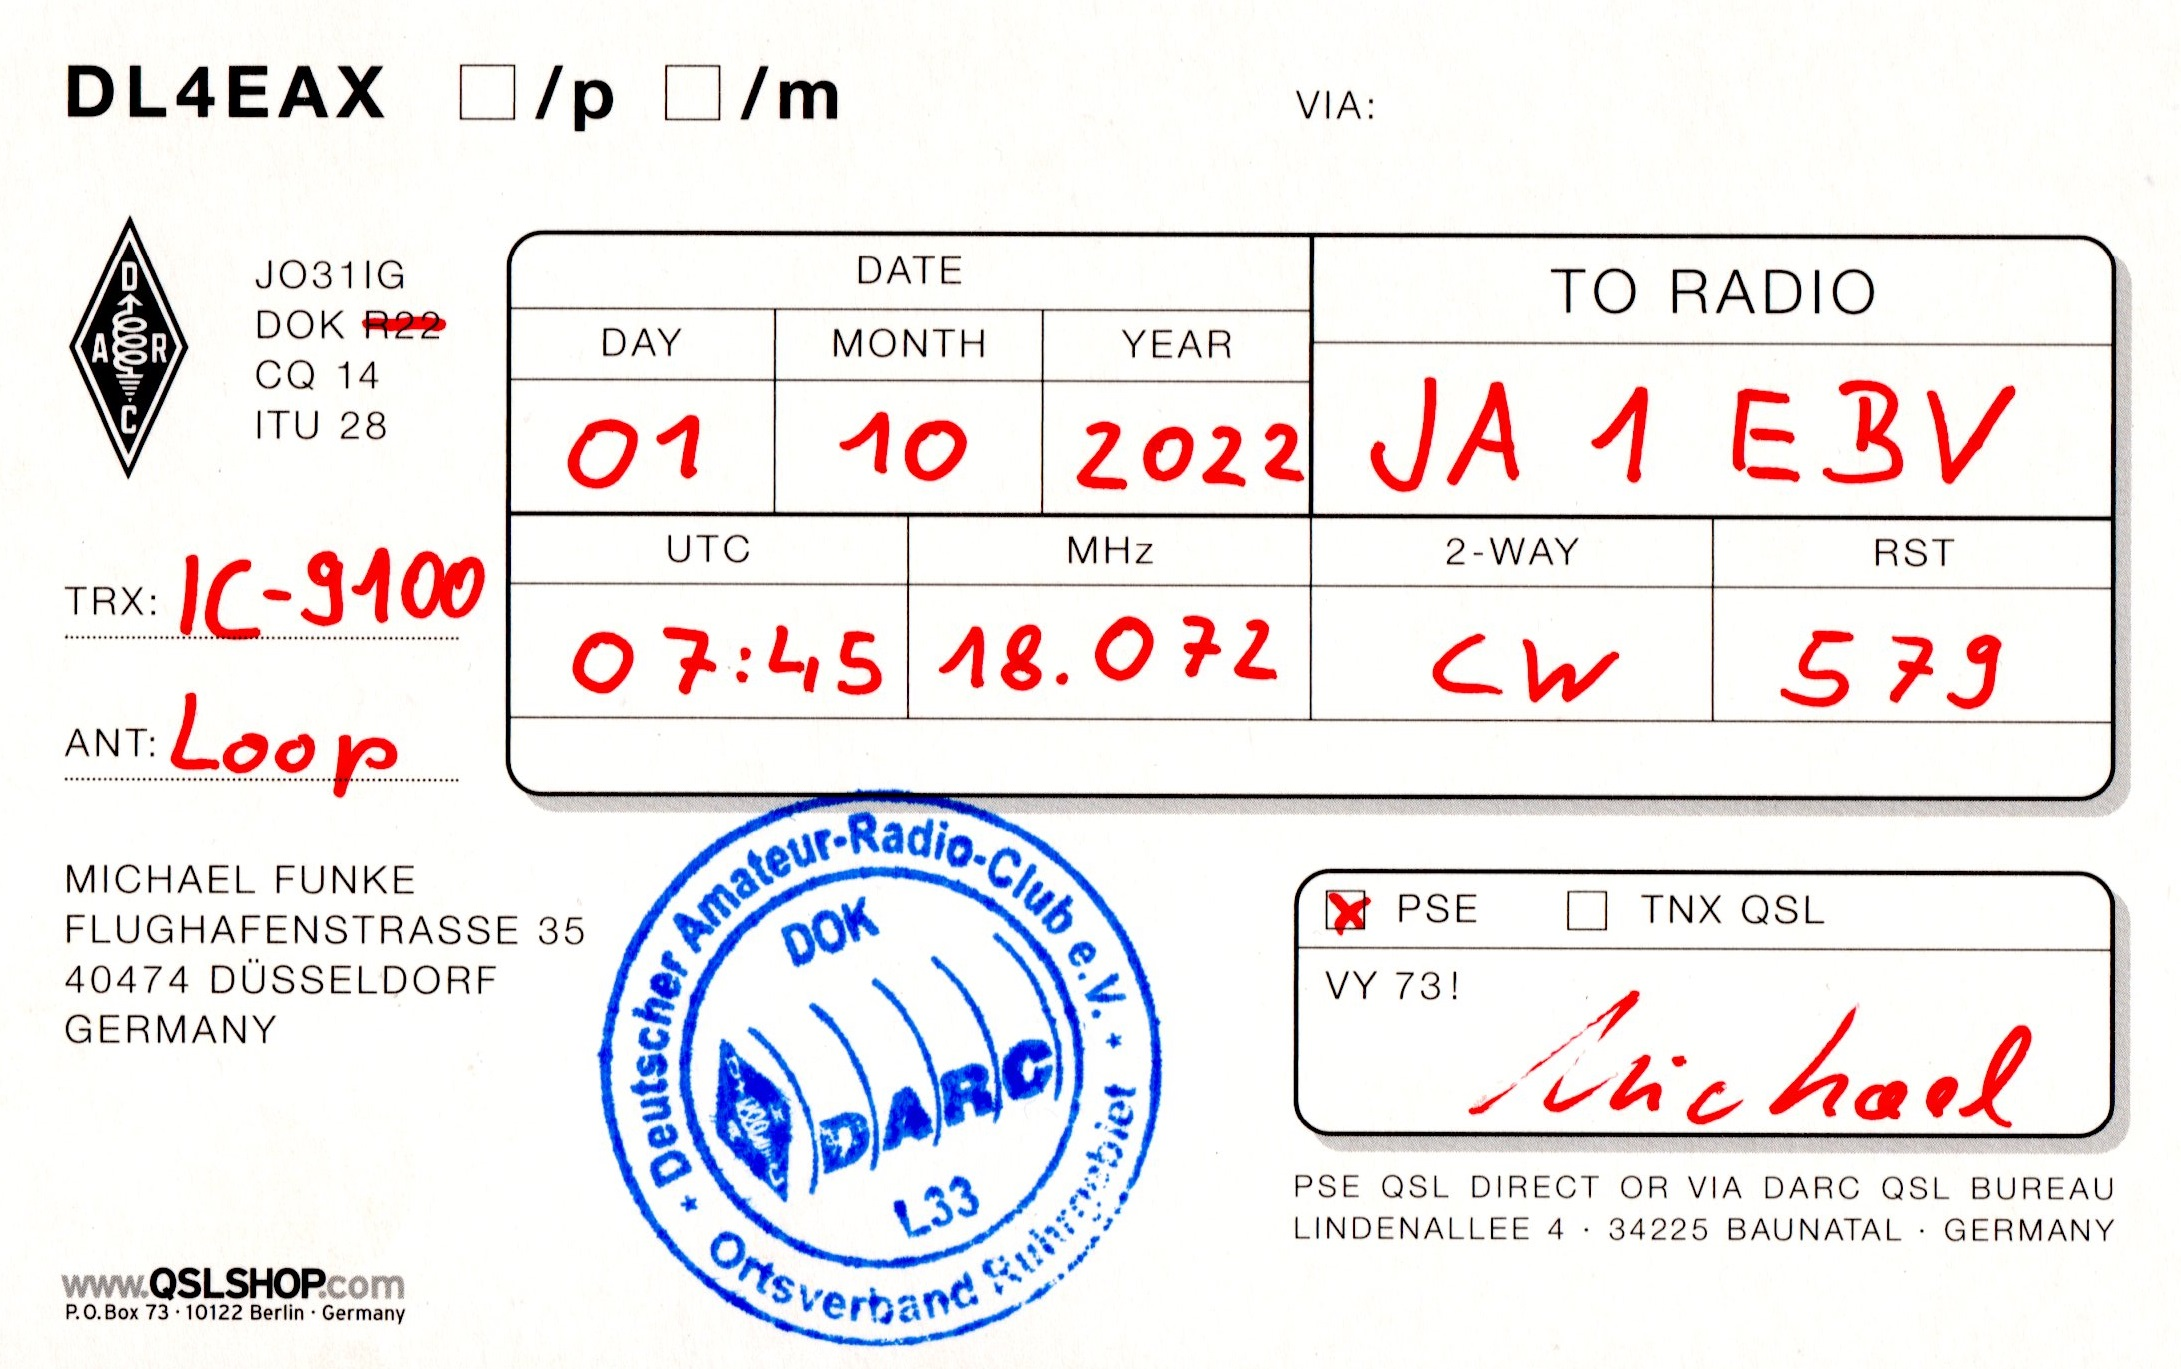
\includegraphics[width=0.85\textwidth]{foto/62}
    \caption{\scriptsize Beispiel für eine QSL-Karte, ausgestellt von DL4EAX zur Bestätigung einer Verbindung mit der Station JA1EBV}
    \label{n_qsl_karten_rueckseite_2}
\end{figure}
\end{frame}

\begin{frame}Eine QSL-Karte sollte mindestens folgende Angaben enthalten:

\begin{itemize}
  \item Datum
  \item Uhrzeit in UTC
  \item Eigenes Rufzeichen
  \item Rufzeichen der Gegenstation
  \item Genutzte Frequenz oder Frequenzband
  \item Verwendetes Übertragungsverfahren
  \item Gegebener Rapport
  \end{itemize}

\end{frame}

\begin{frame}
\only<1>{
\begin{QQuestion}{BG105}{Welche Angaben sollten QSL-Karten \underline{mindestens} enthalten?}{Verwendetes Rufzeichen, Datum und Uhrzeit der Funkverbindung in UTC, Frequenz, Übertragungsverfahren, Signal-Rapport sowie den eigenen Namen, Standort, Locator, die eigene Sendeleistung und Angaben zur eingesetzten technischen Ausrüstung}
{Verwendetes Rufzeichen, Rufzeichen der Gegenstation, Datum und Uhrzeit der Funkverbindung in UTC, Band, Übertragungsverfahren und Signal-Rapport}
{Rufzeichen der Gegenstation, Datum und Uhrzeit der Funkverbindung in UTC, genaue Frequenz, Übertragungsverfahren, Signal-Rapport und weitere übliche Angaben wie den eigenen Namen, Standort, Locator und die eigene Sendeleistung}
{Rufzeichen der Gegenstation, Datum und Uhrzeit der Funkverbindung in UTC, Frequenz, Übertragungsverfahren, Angaben über das Funkwetter und die Unterschrift des Operators}
\end{QQuestion}

}
\only<2>{
\begin{QQuestion}{BG105}{Welche Angaben sollten QSL-Karten \underline{mindestens} enthalten?}{Verwendetes Rufzeichen, Datum und Uhrzeit der Funkverbindung in UTC, Frequenz, Übertragungsverfahren, Signal-Rapport sowie den eigenen Namen, Standort, Locator, die eigene Sendeleistung und Angaben zur eingesetzten technischen Ausrüstung}
{\textbf{\textcolor{DARCgreen}{Verwendetes Rufzeichen, Rufzeichen der Gegenstation, Datum und Uhrzeit der Funkverbindung in UTC, Band, Übertragungsverfahren und Signal-Rapport}}}
{Rufzeichen der Gegenstation, Datum und Uhrzeit der Funkverbindung in UTC, genaue Frequenz, Übertragungsverfahren, Signal-Rapport und weitere übliche Angaben wie den eigenen Namen, Standort, Locator und die eigene Sendeleistung}
{Rufzeichen der Gegenstation, Datum und Uhrzeit der Funkverbindung in UTC, Frequenz, Übertragungsverfahren, Angaben über das Funkwetter und die Unterschrift des Operators}
\end{QQuestion}

}
\end{frame}

\begin{frame}
\only<1>{
\begin{QQuestion}{BG106}{Was sollten Sie bei der Eintragung von Uhrzeiten in QSL-Karten beachten? Sie sollten in~...}{der Ortszeit des Funkpartners eingetragen werden, damit es zu keinen Verwechselungen kommt.}
{der eigenen Ortszeit eingetragen werden, um den deutschen Vorschriften zu genügen.}
{der koordinierten Weltzeit (UTC) eingetragen werden, um Funkpartnern im Ausland das Auffinden im Logbuch zu erleichtern.}
{der eigenen Ortszeit und zusätzlich in der Ortszeit des Funkpartners eingetragen werden, um sowohl den deutschen Vorschriften zu genügen als auch Funkpartnern im Ausland das Auffinden im Logbuch zu erleichtern.}
\end{QQuestion}

}
\only<2>{
\begin{QQuestion}{BG106}{Was sollten Sie bei der Eintragung von Uhrzeiten in QSL-Karten beachten? Sie sollten in~...}{der Ortszeit des Funkpartners eingetragen werden, damit es zu keinen Verwechselungen kommt.}
{der eigenen Ortszeit eingetragen werden, um den deutschen Vorschriften zu genügen.}
{\textbf{\textcolor{DARCgreen}{der koordinierten Weltzeit (UTC) eingetragen werden, um Funkpartnern im Ausland das Auffinden im Logbuch zu erleichtern.}}}
{der eigenen Ortszeit und zusätzlich in der Ortszeit des Funkpartners eingetragen werden, um sowohl den deutschen Vorschriften zu genügen als auch Funkpartnern im Ausland das Auffinden im Logbuch zu erleichtern.}
\end{QQuestion}

}
\end{frame}

\begin{frame}
\only<1>{
\begin{QQuestion}{BG107}{Welche Uhrzeit tragen Sie in die QSL-Karte ein, wenn Sie um 15:30 MEZ ein QSO hatten?}{14:30 UTC}
{13:30 UTC}
{17:30 UTC}
{16:30 UTC}
\end{QQuestion}

}
\only<2>{
\begin{QQuestion}{BG107}{Welche Uhrzeit tragen Sie in die QSL-Karte ein, wenn Sie um 15:30 MEZ ein QSO hatten?}{\textbf{\textcolor{DARCgreen}{14:30 UTC}}}
{13:30 UTC}
{17:30 UTC}
{16:30 UTC}
\end{QQuestion}

}
\end{frame}

\begin{frame}
\only<1>{
\begin{QQuestion}{BG108}{Welche Uhrzeit tragen Sie in die QSL-Karte ein, wenn Sie um 13:30 MESZ eine Funkverbindung hatten?}{11:30 UTC}
{13:30 UTC}
{12:30 UTC}
{14:30 UTC}
\end{QQuestion}

}
\only<2>{
\begin{QQuestion}{BG108}{Welche Uhrzeit tragen Sie in die QSL-Karte ein, wenn Sie um 13:30 MESZ eine Funkverbindung hatten?}{\textbf{\textcolor{DARCgreen}{11:30 UTC}}}
{13:30 UTC}
{12:30 UTC}
{14:30 UTC}
\end{QQuestion}

}
\end{frame}

\begin{frame}
\frametitle{Vermittlung von QSL-Karten}
\begin{itemize}
  \item Über teilnehmende Amateurfunkverbände in den Ländern
  \item via Vermittlungsbüro -- international \enquote{Bureau}
  \item Weltweites alternatives Postnetz
  \item In Deutschland bietet das der DARC e.V. für Mitglieder kostenlos an
  \end{itemize}

\end{frame}

\begin{frame}
\frametitle{Callbooks}
\begin{itemize}
  \item Adressen in internationalen Amateurfunk-Rufzeichenlisten (Callbook)
  \item Oder im Internet
  \item Es gibt \enquote{QSL-Manager}, die für andere Stationen den Versand übernehmen
  \end{itemize}

\end{frame}

\begin{frame}
\only<1>{
\begin{QQuestion}{BG110}{Wo können Sie die Anschriften von ausländischen Funkamateuren finden, denen Sie die QSL-Karte direkt zusenden möchten?}{Ich finde diese in der VO Funk.}
{Ich finde diese in der Amateurfunk-Rufzeichenliste auf den Internetseiten der Bundesnetzagentur.}
{Ich finde diese in der internationalen Amateurfunk-Rufzeichenliste (Callbook) oder aus Informationen des Internets.}
{Ich finde diese im internationalen Telefonbuch.}
\end{QQuestion}

}
\only<2>{
\begin{QQuestion}{BG110}{Wo können Sie die Anschriften von ausländischen Funkamateuren finden, denen Sie die QSL-Karte direkt zusenden möchten?}{Ich finde diese in der VO Funk.}
{Ich finde diese in der Amateurfunk-Rufzeichenliste auf den Internetseiten der Bundesnetzagentur.}
{\textbf{\textcolor{DARCgreen}{Ich finde diese in der internationalen Amateurfunk-Rufzeichenliste (Callbook) oder aus Informationen des Internets.}}}
{Ich finde diese im internationalen Telefonbuch.}
\end{QQuestion}

}
\end{frame}

\begin{frame}
\only<1>{
\begin{QQuestion}{BG109}{HZ1HZ sagte Ihnen \glqq QSL via K8PYD\grqq{}. Was würden Sie tun, um die QSL-Karte von HZ1HZ zu erhalten?}{Ich warte, bis HZ1HZ die Karte an K8PYD geschickt hat.}
{Ich muss meine QSL-Karte via HZ1HZ senden, weil K8PYD der QSO-Partner war.}
{Ich schaue im Callbook nach der Adresse von HZ1HZ und schicke die Karte direkt.}
{Ich sende meine QSL-Karte via K8PYD, weil dieser der QSL-Manager von HZ1HZ ist.}
\end{QQuestion}

}
\only<2>{
\begin{QQuestion}{BG109}{HZ1HZ sagte Ihnen \glqq QSL via K8PYD\grqq{}. Was würden Sie tun, um die QSL-Karte von HZ1HZ zu erhalten?}{Ich warte, bis HZ1HZ die Karte an K8PYD geschickt hat.}
{Ich muss meine QSL-Karte via HZ1HZ senden, weil K8PYD der QSO-Partner war.}
{Ich schaue im Callbook nach der Adresse von HZ1HZ und schicke die Karte direkt.}
{\textbf{\textcolor{DARCgreen}{Ich sende meine QSL-Karte via K8PYD, weil dieser der QSL-Manager von HZ1HZ ist.}}}
\end{QQuestion}

}
\end{frame}

\begin{frame}
\frametitle{Elektronische QSL-Karten}
\begin{itemize}
  \item Papierlose Alternativen
  \item Elektronische Logbücher lassen sich hochladen
  \item Nur wenige Plattformen werden für Diplome anerkannt
  \end{itemize}
\end{frame}

\begin{frame}
\only<1>{
\begin{QQuestion}{BG111}{Welche Alternativen zur QSL-Karte sind üblich? Bestätigung von Funkverbindungen durch~...}{elektronische QSL-Karten oder Logbuch-Upload}
{die BNetzA als unabhängige Stelle}
{das Intruder Monitoring der Amateurfunkverbände}
{Beurkundung durch einen Notar oder SWL-Fachanwalt}
\end{QQuestion}

}
\only<2>{
\begin{QQuestion}{BG111}{Welche Alternativen zur QSL-Karte sind üblich? Bestätigung von Funkverbindungen durch~...}{\textbf{\textcolor{DARCgreen}{elektronische QSL-Karten oder Logbuch-Upload}}}
{die BNetzA als unabhängige Stelle}
{das Intruder Monitoring der Amateurfunkverbände}
{Beurkundung durch einen Notar oder SWL-Fachanwalt}
\end{QQuestion}

}
\end{frame}%ENDCONTENT


\title{DARC Amateurfunklehrgang Klasse N}
\author{Betriebsabwicklung}
\institute{Deutscher Amateur Radio Club e.\,V.}
\begin{frame}
\maketitle
\end{frame}

\section{Pile-up}
\label{section:pileup}
\begin{frame}%STARTCONTENT

\frametitle{Was ist ein Pile-Up?}
\begin{itemize}
  \item Der Begriff Pile-Up kommt vom englischen Verb \enquote{to pile up}, was soviel bedeutet wie \enquote{sich aufstapeln}.
  \item Was sich hier aufstapelt, sind die immer mehr werdenden Funkamateure, die alle das gleiche Ziel verfolgen: Eine Verbindung mit der begehrten Station herzustellen.
  \end{itemize}

\end{frame}

\begin{frame}
\frametitle{Umgang mit dem Pile-Up 1}
\begin{itemize}
  \item Manchmal wird der CQ-Ruf auf bestimmte Ziffern im Rufzeichen beschränkt, zum Beispiel \enquote{\emph{only number}~5}.
  \item Oder der Aufruf wird nach Ländern oder Kontinenten vorgenommen, zum Beispiel \enquote{Asia only}
  \item Selten wird \emph{Listenbetrieb} gemacht: Eine andere Station nimmt die Kontaktwünsche auf und erstellt eine Liste, die von der begehrten Station abgearbeitet wird.
  \end{itemize}
\end{frame}

\begin{frame}
\only<1>{
\begin{QQuestion}{BE305}{Was ist mit dem Begriff \glqq pile up\grqq{} gemeint? Im Amateurfunk meint man damit das gleichzeitige~...}{Anrufen einer begehrten Station durch viele Amateurfunkstellen.}
{Senden einer Station auf mehreren Amateurfunkfrequenzen.}
{Peilen einer Station mit mehreren übereinander angeordneten Richtantennen.}
{Hören einer Station mit vielen Remote-Stationen bei einem Contest.}
\end{QQuestion}

}
\only<2>{
\begin{QQuestion}{BE305}{Was ist mit dem Begriff \glqq pile up\grqq{} gemeint? Im Amateurfunk meint man damit das gleichzeitige~...}{\textbf{\textcolor{DARCgreen}{Anrufen einer begehrten Station durch viele Amateurfunkstellen.}}}
{Senden einer Station auf mehreren Amateurfunkfrequenzen.}
{Peilen einer Station mit mehreren übereinander angeordneten Richtantennen.}
{Hören einer Station mit vielen Remote-Stationen bei einem Contest.}
\end{QQuestion}

}
\end{frame}

\begin{frame}
\only<1>{
\begin{QQuestion}{BE306}{Eine begehrte Station ruft in Telefonie \glqq only number 3\grqq{}. Was ist damit gemeint? Die Station~...}{möchte, dass anrufende Stationen dreimal ihren Suffix durchgeben.}
{möchte jeweils drei rufende Stationen in eine Liste aufnehmen.}
{möchte Stationen mit dreistelligem Suffix aufrufen.}
{möchte Anrufe von Stationen mit der Ziffer 3 zwischen Präfix und Suffix.}
\end{QQuestion}

}
\only<2>{
\begin{QQuestion}{BE306}{Eine begehrte Station ruft in Telefonie \glqq only number 3\grqq{}. Was ist damit gemeint? Die Station~...}{möchte, dass anrufende Stationen dreimal ihren Suffix durchgeben.}
{möchte jeweils drei rufende Stationen in eine Liste aufnehmen.}
{möchte Stationen mit dreistelligem Suffix aufrufen.}
{\textbf{\textcolor{DARCgreen}{möchte Anrufe von Stationen mit der Ziffer 3 zwischen Präfix und Suffix.}}}
\end{QQuestion}

}
\end{frame}

\begin{frame}
\only<1>{
\begin{QQuestion}{BE307}{Was verstehen Sie bei einer seltenen Station unter der Aufforderung zu \glqq Listenbetrieb\grqq{}?}{Eine gut hörbare andere Station nimmt anrufende Stationen in eine Liste und ruft später diese Stationen zur Aufnahme einer Funkverbindung mit der seltenen Station auf.}
{Eine gut hörbare andere Station schickt per Internet Listen anrufender Stationen an die seltene Station.}
{Die seltene Station ruft Stationen nach einer Liste der Landeskenner alphabetisch auf.}
{Die seltene Station oder ihr QSL-Manager veröffentlicht eine Liste der gearbeiteten Stationen in den Amateurfunkzeitschriften.}
\end{QQuestion}

}
\only<2>{
\begin{QQuestion}{BE307}{Was verstehen Sie bei einer seltenen Station unter der Aufforderung zu \glqq Listenbetrieb\grqq{}?}{\textbf{\textcolor{DARCgreen}{Eine gut hörbare andere Station nimmt anrufende Stationen in eine Liste und ruft später diese Stationen zur Aufnahme einer Funkverbindung mit der seltenen Station auf.}}}
{Eine gut hörbare andere Station schickt per Internet Listen anrufender Stationen an die seltene Station.}
{Die seltene Station ruft Stationen nach einer Liste der Landeskenner alphabetisch auf.}
{Die seltene Station oder ihr QSL-Manager veröffentlicht eine Liste der gearbeiteten Stationen in den Amateurfunkzeitschriften.}
\end{QQuestion}

}
\end{frame}%ENDCONTENT


\section{Split-Verkehr}
\label{section:split_betrieb}
\begin{frame}%STARTCONTENT

\frametitle{Umgang mit dem Pile-Up 2}
\begin{itemize}
  \item Split-Verkehr ist die am Meisten genutzte Methode um vielen Anrufen eine Verbindung zu ermöglichen.
  \item Dabei empfängt die begehrte Station auf einer anderen Frequenz als sie sendet.
  \item Die CQ-rufende Station kündigt den Split-Verkehr mit Hinweis auf die Frequenz oder den Frequenzbereich an, in dem sie empfängt. Zum Beispiel \enquote{5 up} oder \enquote{split 14270 to 14280}.
  \end{itemize}

\end{frame}

\begin{frame}
\begin{figure}
    \DARCimage{0.85\linewidth}{672include}
    \caption{\scriptsize Split-Verkehr, Sendefrequenz der begehrten Station und Antwort-Frequenz, auf der sie empfängt}
    \label{n_split_verkehr_anruffrequenz}
\end{figure}


\begin{figure}
    \DARCimage{0.85\linewidth}{673include}
    \caption{\scriptsize Split-Verkehr, Sendefrequenz der begehrten Station und Frequenzbereich für Antworten, in dem sie empfängt}
    \label{n_split_verkehr_anrufbereich}
\end{figure}

\end{frame}

\begin{frame}
\only<1>{
\begin{QQuestion}{BE308}{Was ist \glqq Split-Verkehr\grqq{}?}{Nutzung unterschiedlicher Übertragungsverfahren in einem QSO}
{Verwenden von mehr als einem Funkgerät}
{Teilen einer Frequenz zwischen zwei Relaisfunkstellen}
{Senden und Empfangen auf unterschiedlichen Frequenzen}
\end{QQuestion}

}
\only<2>{
\begin{QQuestion}{BE308}{Was ist \glqq Split-Verkehr\grqq{}?}{Nutzung unterschiedlicher Übertragungsverfahren in einem QSO}
{Verwenden von mehr als einem Funkgerät}
{Teilen einer Frequenz zwischen zwei Relaisfunkstellen}
{\textbf{\textcolor{DARCgreen}{Senden und Empfangen auf unterschiedlichen Frequenzen}}}
\end{QQuestion}

}
\end{frame}

\begin{frame}
\only<1>{
\begin{QQuestion}{BE310}{Eine Station gibt am Ende ihres CQ-Rufes \glqq 5 up\grqq{}. Was bedeutet diese Angabe und was ist zu beachten?}{Die rufende Station behandelt meinen Anruf an 5ter Stelle. Ich muss also bei meinem Anruf 4 andere Funkverbindungen abwarten.}
{Die rufende Station hört 5~Minuten später auf ihrer eigenen Sendefrequenz. Ich muss also bei meinem Anruf 5~Minuten später senden und vorher prüfen, ob die Frequenz frei ist.}
{Die rufende Station sendet \qty{5}{\kHz} oberhalb ihrer eigenen Sendefrequenz. Ich muss also bei meinem Anruf \qty{5}{\kHz} höher empfangen und vorher prüfen, ob die Frequenz frei ist.}
{Die rufende Station hört \qty{5}{\kHz} oberhalb ihrer eigenen Sendefrequenz. Ich muss also bei meinem Anruf \qty{5}{\kHz} höher senden.}
\end{QQuestion}

}
\only<2>{
\begin{QQuestion}{BE310}{Eine Station gibt am Ende ihres CQ-Rufes \glqq 5 up\grqq{}. Was bedeutet diese Angabe und was ist zu beachten?}{Die rufende Station behandelt meinen Anruf an 5ter Stelle. Ich muss also bei meinem Anruf 4 andere Funkverbindungen abwarten.}
{Die rufende Station hört 5~Minuten später auf ihrer eigenen Sendefrequenz. Ich muss also bei meinem Anruf 5~Minuten später senden und vorher prüfen, ob die Frequenz frei ist.}
{Die rufende Station sendet \qty{5}{\kHz} oberhalb ihrer eigenen Sendefrequenz. Ich muss also bei meinem Anruf \qty{5}{\kHz} höher empfangen und vorher prüfen, ob die Frequenz frei ist.}
{\textbf{\textcolor{DARCgreen}{Die rufende Station hört \qty{5}{\kHz} oberhalb ihrer eigenen Sendefrequenz. Ich muss also bei meinem Anruf \qty{5}{\kHz} höher senden.}}}
\end{QQuestion}

}
\end{frame}

\begin{frame}
\only<1>{
\begin{QQuestion}{BE309}{Was bedeutet es, wenn eine begehrte Station CQ ruft und den Anruf mit \glqq split up 14270 to 14280\grqq{} beendet? Die Station~...}{wird im angegebenen Bereich mit einer Bandbreite von \qty{10}{\kHz} senden.}
{kündigt einen Wechsel ihrer Sendefrequenz in den angegebenen Bereich an.}
{bittet anrufende Stationen in dem angegebenen Bereich CW zu verwenden.}
{hört oberhalb ihrer Sendefrequenz auf wechselnden Frequenzen im angegebenen Bereich.}
\end{QQuestion}

}
\only<2>{
\begin{QQuestion}{BE309}{Was bedeutet es, wenn eine begehrte Station CQ ruft und den Anruf mit \glqq split up 14270 to 14280\grqq{} beendet? Die Station~...}{wird im angegebenen Bereich mit einer Bandbreite von \qty{10}{\kHz} senden.}
{kündigt einen Wechsel ihrer Sendefrequenz in den angegebenen Bereich an.}
{bittet anrufende Stationen in dem angegebenen Bereich CW zu verwenden.}
{\textbf{\textcolor{DARCgreen}{hört oberhalb ihrer Sendefrequenz auf wechselnden Frequenzen im angegebenen Bereich.}}}
\end{QQuestion}

}
\end{frame}

\begin{frame}
\only<1>{
\begin{QQuestion}{BE311}{Eine Station, die auf \qty{14205}{\kHz} CQ gerufen hat, sagt am Ende ihres Rufes \glqq tuning 290 to 300 up\grqq{}. Welche Frequenzen nutzen Sie, wenn Sie diese Station anrufen wollen?}{Ich rufe zwischen \num{14290} und \qty{14300}{\kHz} und höre auf \qty{14205}{\kHz}.}
{Ich rufe und höre zwischen \num{14290} und \qty{14300}{\kHz}.}
{Ich rufe auf \qty{14205}{\kHz} und höre zwischen \num{14290} und \qty{14300}{\kHz}.}
{Ich rufe auf \qty{14290}{\kHz} und höre auf \qty{14300}{\kHz}.}
\end{QQuestion}

}
\only<2>{
\begin{QQuestion}{BE311}{Eine Station, die auf \qty{14205}{\kHz} CQ gerufen hat, sagt am Ende ihres Rufes \glqq tuning 290 to 300 up\grqq{}. Welche Frequenzen nutzen Sie, wenn Sie diese Station anrufen wollen?}{\textbf{\textcolor{DARCgreen}{Ich rufe zwischen \num{14290} und \qty{14300}{\kHz} und höre auf \qty{14205}{\kHz}.}}}
{Ich rufe und höre zwischen \num{14290} und \qty{14300}{\kHz}.}
{Ich rufe auf \qty{14205}{\kHz} und höre zwischen \num{14290} und \qty{14300}{\kHz}.}
{Ich rufe auf \qty{14290}{\kHz} und höre auf \qty{14300}{\kHz}.}
\end{QQuestion}

}
\end{frame}%ENDCONTENT


\section{Contest}
\label{section:contest}
\begin{frame}%STARTCONTENT

\frametitle{Was ist ein Contest?}
\begin{itemize}
  \item Im Amateurfunk finden auch Wettbewerbe statt, die als Contest bezeichnet werden.
  \item Conteste dienen dem sportlichen Wettkampf, aber auch dazu, die eigene Amateurfunkstation und Betriebsabwicklung zu verbessern.
  \end{itemize}
\end{frame}

\begin{frame}
\only<1>{
\begin{QQuestion}{BE301}{Was ist der Zweck eines Amateurfunkwettbewerbs (Contest)? Er dient dem Wettkampf und~...}{dem Gewinnen von Preisgeldern.}
{der stetigen Verbesserung von Amateurfunkanlagen und Betriebstechnik.}
{der Erlangung eines Amateurfunkzeugnisses.}
{dem Testen der Störfestigkeit der Empfangsgeräte der Nachbarn.}
\end{QQuestion}

}
\only<2>{
\begin{QQuestion}{BE301}{Was ist der Zweck eines Amateurfunkwettbewerbs (Contest)? Er dient dem Wettkampf und~...}{dem Gewinnen von Preisgeldern.}
{\textbf{\textcolor{DARCgreen}{der stetigen Verbesserung von Amateurfunkanlagen und Betriebstechnik.}}}
{der Erlangung eines Amateurfunkzeugnisses.}
{dem Testen der Störfestigkeit der Empfangsgeräte der Nachbarn.}
\end{QQuestion}

}
\end{frame}

\begin{frame}
\frametitle{Was zeichnet Contestverbindungen aus?}
\begin{itemize}
  \item Die Verbindungen sind besonders kurz, weil man in der vorgegebenen Zeitdauer möglichst viele Verbindungen herstellen möchte.
  \end{itemize}
\end{frame}

\begin{frame}
\only<1>{
\begin{QQuestion}{BE302}{Warum ist der Informationsaustausch bei Verbindungen in einem Amateurfunkwettbewerb (Contest) besonders kurz?}{Um die vorgegebene Zeitbegrenzung für eine einzelne Verbindung einzuhalten.}
{Um in der vorgegebenen Zeitdauer möglichst viele Verbindungen herzustellen.}
{Weil sonst die Disqualifikation droht.}
{Weil alle notwendigen Informationen auch im Internet auffindbar sind.}
\end{QQuestion}

}
\only<2>{
\begin{QQuestion}{BE302}{Warum ist der Informationsaustausch bei Verbindungen in einem Amateurfunkwettbewerb (Contest) besonders kurz?}{Um die vorgegebene Zeitbegrenzung für eine einzelne Verbindung einzuhalten.}
{\textbf{\textcolor{DARCgreen}{Um in der vorgegebenen Zeitdauer möglichst viele Verbindungen herzustellen.}}}
{Weil sonst die Disqualifikation droht.}
{Weil alle notwendigen Informationen auch im Internet auffindbar sind.}
\end{QQuestion}

}
\end{frame}

\begin{frame}
\frametitle{Woran erkennt man Conteststationen?}
\begin{itemize}
  \item Oft erkennt man Conteststationen daran, dass der Namen des Wettbewerbes oder einfach nur \enquote{CONTEST} in den CQ-Ruf integriert wird.
  \item Zum Beispiel: \enquote{CQ FD} oder \enquote{CQ Ruhrgebietscontest} oder \enquote{CQ Contest}.
  \item In Telegrafie dann CQ TEST.
  \end{itemize}

\end{frame}

\begin{frame}
\only<1>{
\begin{QQuestion}{BE116}{Sie hören in Telegrafie \glqq CQ FD DD4UQ/P TEST\grqq{}. Was bedeutet das? Die Station DD4UQ~...}{sucht Verbindungen mit Stationen aus dem Raum Fulda.}
{sucht Verbindungen mit Stationen, die am Fieldday-Contest teilnehmen.}
{führt Testaussendungen im Full-Duplex-Betrieb durch.}
{führt Testaussendungen des Fernmeldedienstes durch.}
\end{QQuestion}

}
\only<2>{
\begin{QQuestion}{BE116}{Sie hören in Telegrafie \glqq CQ FD DD4UQ/P TEST\grqq{}. Was bedeutet das? Die Station DD4UQ~...}{sucht Verbindungen mit Stationen aus dem Raum Fulda.}
{\textbf{\textcolor{DARCgreen}{sucht Verbindungen mit Stationen, die am Fieldday-Contest teilnehmen.}}}
{führt Testaussendungen im Full-Duplex-Betrieb durch.}
{führt Testaussendungen des Fernmeldedienstes durch.}
\end{QQuestion}

}
\end{frame}

\begin{frame}
\frametitle{Besondere Betriebsabwicklung im Contest}
\begin{itemize}
  \item Welche Daten ausgetauscht werden, kann man der Ausschreibung entnehmen.
  \item Es gibt Wettbewerbe, bei denen nach jeder Verbindung die CQ-rufende Station die Frequenz der Gegenstation überlassen muss. Diese werden oft als \enquote{Sprint Contest} bezeichnet, ein Blick in Ausschreibung ist angeraten.
  \end{itemize}
\end{frame}

\begin{frame}
\only<1>{
\begin{QQuestion}{BE303}{Sie nehmen an einem Amateurfunkwettbewerb (Contest) teil. Welche Informationen sollten Sie in einem QSO austauschen?}{Ich beschränke mich auf das Rufzeichen, damit ich schnell möglichst viele Verbindungen erzielen kann.}
{Ich sende Rufzeichen, Signalrapport, Name, Standort und Stationsbeschreibung, damit das Logbuch der Gegenstation vollständig ist.}
{Ich entscheide für jede Verbindung einzeln, welche Daten ich sende, damit ich nicht zu viel über mich preisgebe.}
{Ich übermittle die in der Ausschreibung festgelegten Daten, damit die Verbindung gewertet wird.}
\end{QQuestion}

}
\only<2>{
\begin{QQuestion}{BE303}{Sie nehmen an einem Amateurfunkwettbewerb (Contest) teil. Welche Informationen sollten Sie in einem QSO austauschen?}{Ich beschränke mich auf das Rufzeichen, damit ich schnell möglichst viele Verbindungen erzielen kann.}
{Ich sende Rufzeichen, Signalrapport, Name, Standort und Stationsbeschreibung, damit das Logbuch der Gegenstation vollständig ist.}
{Ich entscheide für jede Verbindung einzeln, welche Daten ich sende, damit ich nicht zu viel über mich preisgebe.}
{\textbf{\textcolor{DARCgreen}{Ich übermittle die in der Ausschreibung festgelegten Daten, damit die Verbindung gewertet wird.}}}
\end{QQuestion}

}
\end{frame}

\begin{frame}
\only<1>{
\begin{QQuestion}{BE304}{Welche besondere Regelung gilt in einem \glqq Sprint-Contest\grqq{}?}{Die Teilnehmer müssen während des Funkbetriebs in ständiger Bewegung bleiben.}
{Es wird in Telegrafie gearbeitet und die Geschwindigkeit, mit der gegeben wird, fließt in die Wertung ein.}
{Das Rufzeichen darf nicht buchstabiert werden, außer am Anfang und am Ende des Wettbewerbs.}
{Nach jeder Verbindung überlässt die CQ-rufende Station die Frequenz der Gegenstation.}
\end{QQuestion}

}
\only<2>{
\begin{QQuestion}{BE304}{Welche besondere Regelung gilt in einem \glqq Sprint-Contest\grqq{}?}{Die Teilnehmer müssen während des Funkbetriebs in ständiger Bewegung bleiben.}
{Es wird in Telegrafie gearbeitet und die Geschwindigkeit, mit der gegeben wird, fließt in die Wertung ein.}
{Das Rufzeichen darf nicht buchstabiert werden, außer am Anfang und am Ende des Wettbewerbs.}
{\textbf{\textcolor{DARCgreen}{Nach jeder Verbindung überlässt die CQ-rufende Station die Frequenz der Gegenstation.}}}
\end{QQuestion}

}
\end{frame}%ENDCONTENT


\section{Fuchsjagd (ARDF)}
\label{section:ardf}
\begin{frame}%STARTCONTENT

\frametitle{Fuchsjagd (ARDF)}
\begin{itemize}
  \item Eine weitere Art von Wettbewerb ist das Amateur Radio Direction Finding (ARDF).
  \item Die „Füchse“ sind kleine versteckte Sender, die von den Teilnehmern mittels Peilempfängern gefunden und zu Fuß angelaufen werden müssen.
  \item Die Füchse senden im zeitlichem Wechsel jeweils ein anderes der folgende Rufzeichen in CW-Morsetelegrafie aus: MO, MOE, MOI, MOS, MOH oder MO5.
  \end{itemize}
\end{frame}

\begin{frame}
\frametitle{Rufzeichen der Fuchsjagdsender}
\begin{columns}
    \begin{column}{0.48\textwidth}
    \begin{table}
\begin{DARCtabular}{ll}
     Rufzeichen  & Morse-Code   \\
     MO  & \MorseDah\MorseDah\MorseCharSep\MorseDah\MorseDah\MorseDah   \\
     MOE  & \MorseDah\MorseDah\MorseCharSep\MorseDah\MorseDah\MorseDah\MorseCharSep\MorseDit   \\
     MOI  & \MorseDah\MorseDah\MorseCharSep\MorseDah\MorseDah\MorseDah\MorseCharSep\MorseDit\MorseDit   \\
     MOS  & \MorseDah\MorseDah\MorseCharSep\MorseDah\MorseDah\MorseDah\MorseCharSep\MorseDit\MorseDit\MorseDit   \\
     MOH  & \MorseDah\MorseDah\MorseCharSep\MorseDah\MorseDah\MorseDah\MorseCharSep\MorseDit\MorseDit\MorseDit\MorseDit   \\
     MO5  & \MorseDah\MorseDah\MorseCharSep\MorseDah\MorseDah\MorseDah\MorseCharSep\MorseDit\MorseDit\MorseDit\MorseDit\MorseDit   \\
\end{DARCtabular}
\caption{Rufzeichen der Fuchsjagdsender}
\label{ardf_morse_code}
\end{table}

    \end{column}
   \begin{column}{0.48\textwidth}
       
\begin{figure}
    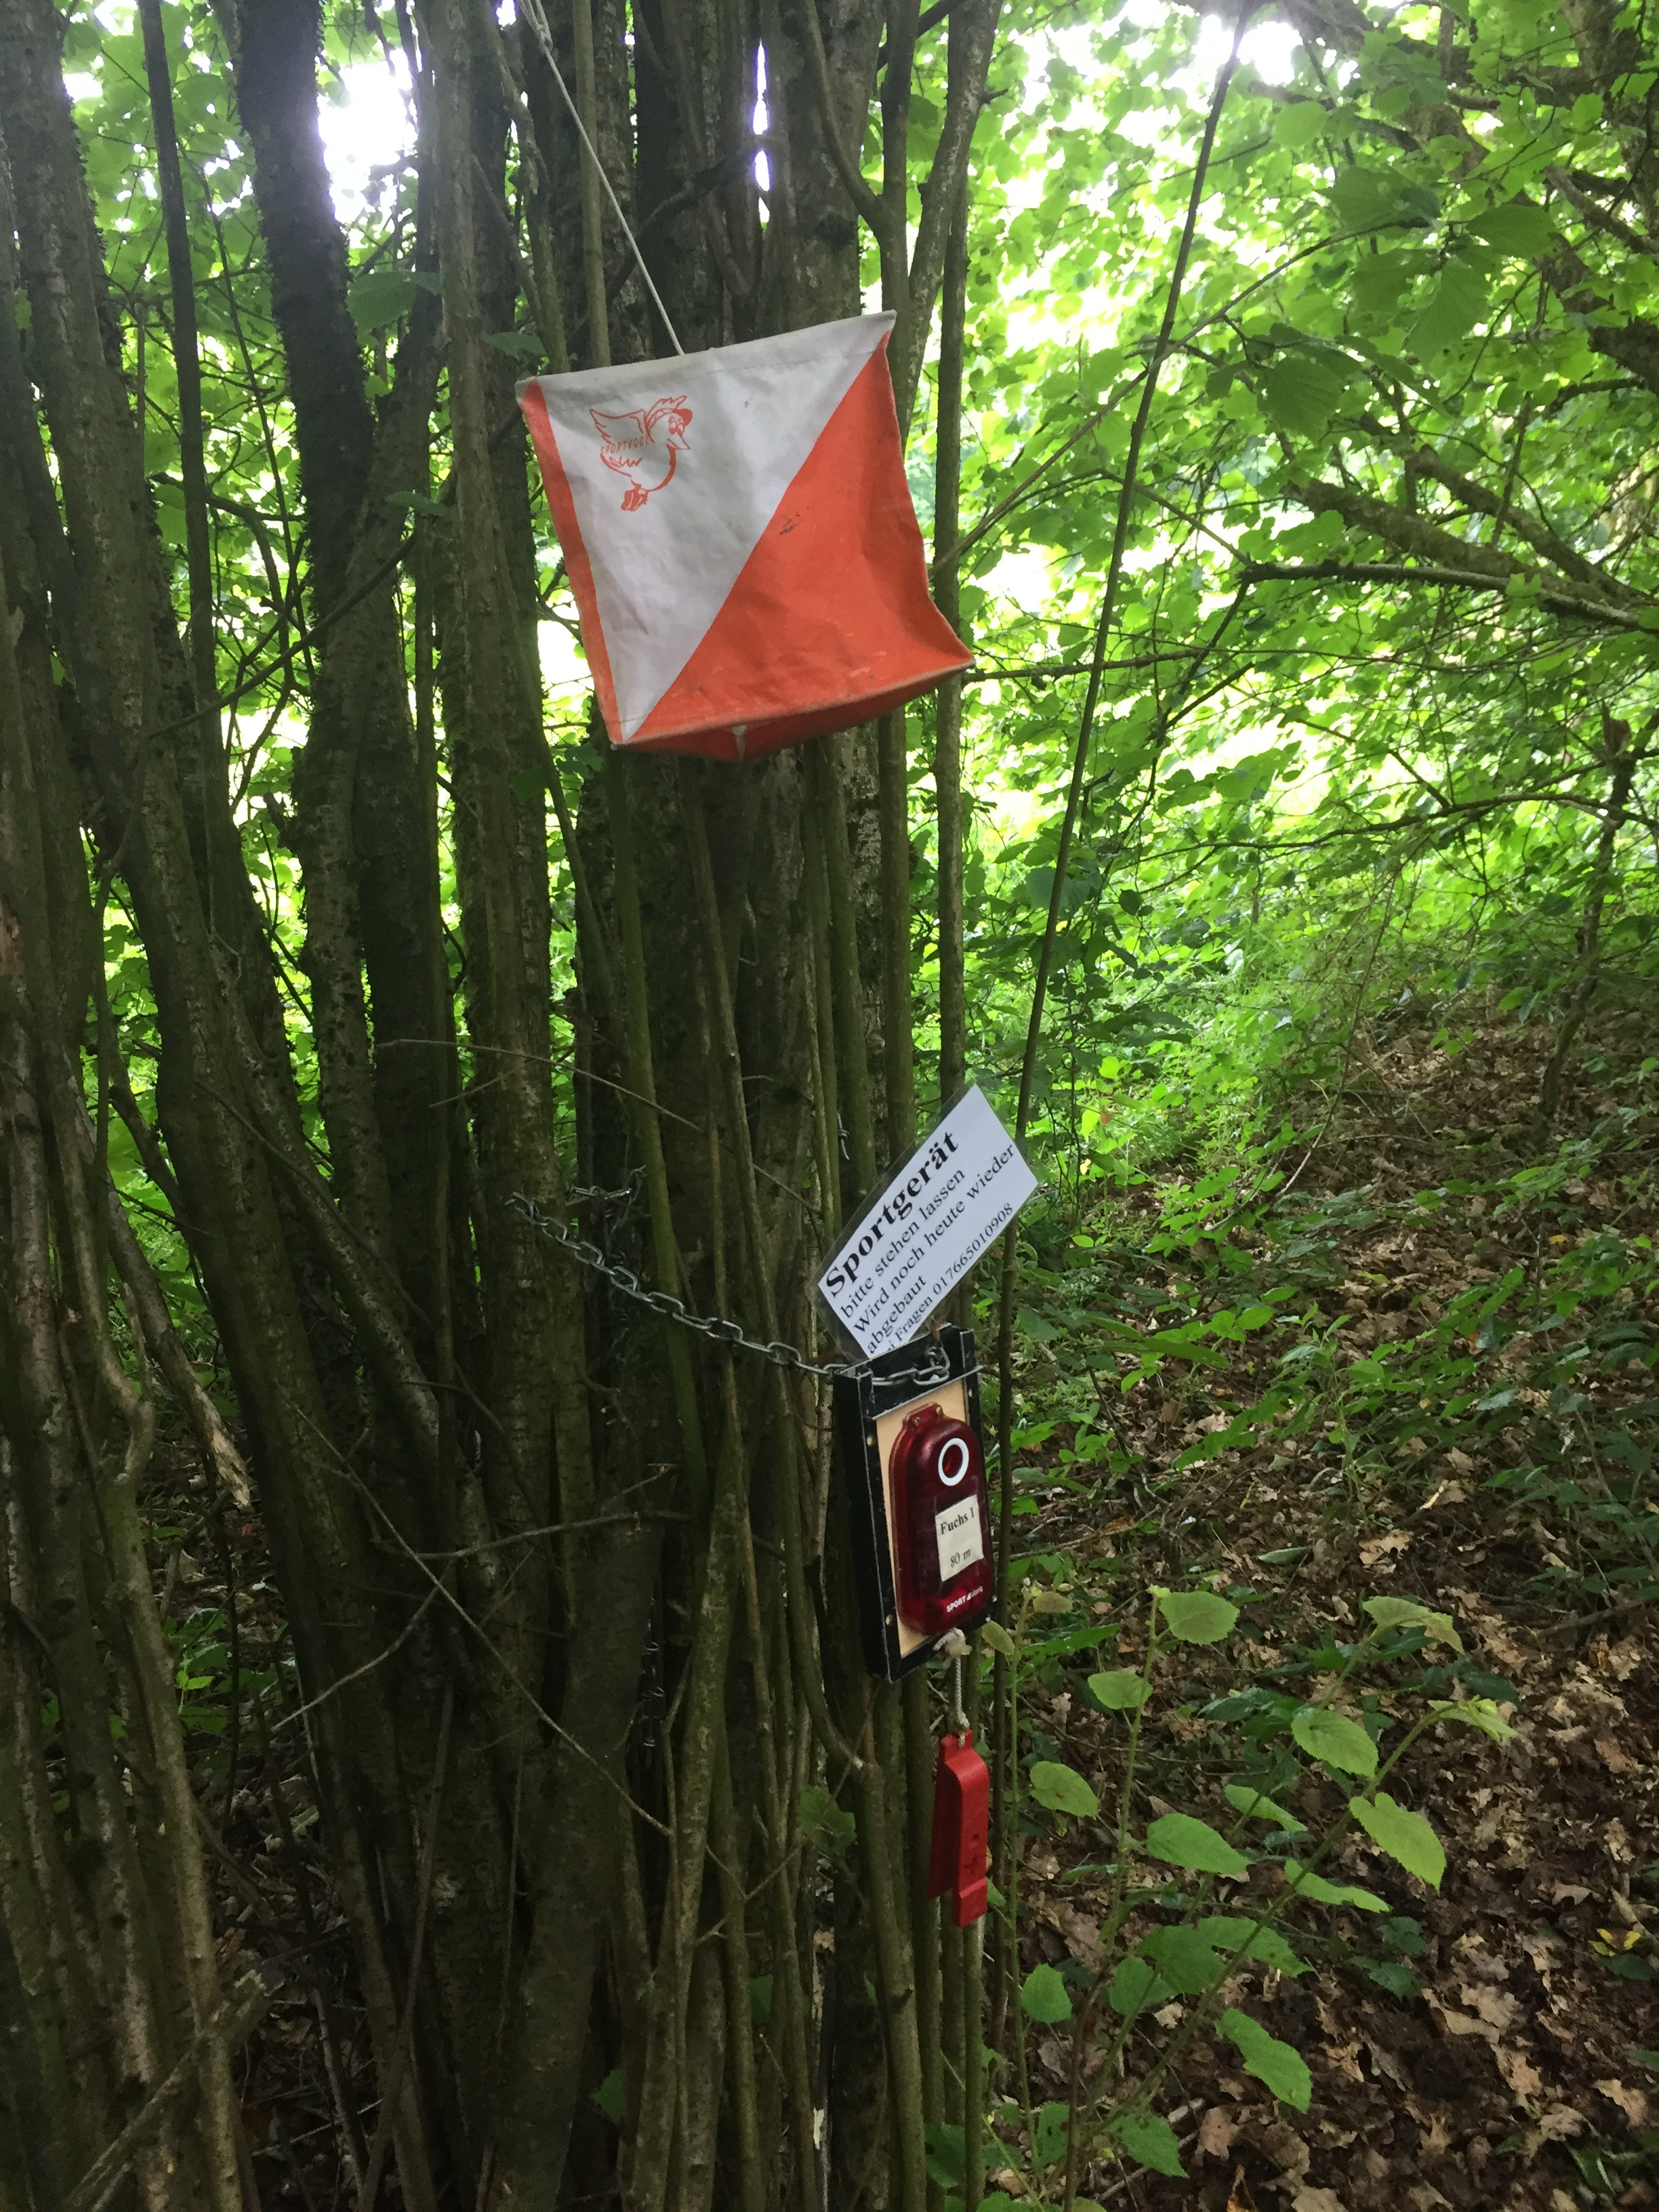
\includegraphics[width=0.85\textwidth]{foto/190}
    \caption{\scriptsize ARDF-Fuchs im Wald mit Wimpel und Zeitnehmer}
    \label{n_ardf_fuchs}
\end{figure}

   \end{column}
\end{columns}

\end{frame}

\begin{frame}
\only<1>{
\begin{QQuestion}{BE313}{Was verstehen Funkamateure unter einer \glqq Fuchsjagd\grqq{} (ARDF = Amateur Radio Direction Finding)?}{Es ist ein Funkwettbewerb, wobei versucht wird, in einer vorgegebenen Zeit auf einem Amateurfunkband mit möglichst vielen Ländern Funkverbindungen herzustellen.}
{Es ist ein Funkpeilwettbewerb, wobei mit Hilfe von tragbaren Peilempfängern versteckte Kleinsender im KW- oder UKW-Bereich, die nur kurzzeitig senden, aufzufinden sind.}
{Bei der Fuchsjagd wird versucht, den Weg von mobilen Kleinsendern zu verfolgen und dabei ein Muster zu erkennen.}
{Es ist ein Funkpeilwettbewerb, der von Funkamateuren ausschließlich für SWL's (short wave listeners) veranstaltet wird. }
\end{QQuestion}

}
\only<2>{
\begin{QQuestion}{BE313}{Was verstehen Funkamateure unter einer \glqq Fuchsjagd\grqq{} (ARDF = Amateur Radio Direction Finding)?}{Es ist ein Funkwettbewerb, wobei versucht wird, in einer vorgegebenen Zeit auf einem Amateurfunkband mit möglichst vielen Ländern Funkverbindungen herzustellen.}
{\textbf{\textcolor{DARCgreen}{Es ist ein Funkpeilwettbewerb, wobei mit Hilfe von tragbaren Peilempfängern versteckte Kleinsender im KW- oder UKW-Bereich, die nur kurzzeitig senden, aufzufinden sind.}}}
{Bei der Fuchsjagd wird versucht, den Weg von mobilen Kleinsendern zu verfolgen und dabei ein Muster zu erkennen.}
{Es ist ein Funkpeilwettbewerb, der von Funkamateuren ausschließlich für SWL's (short wave listeners) veranstaltet wird. }
\end{QQuestion}

}
\end{frame}

\begin{frame}
\only<1>{
\begin{QQuestion}{BD109}{Welche Kennungen werden von leistungsschwachen Amateurfunksendern zu Peilzwecken ausgesendet?}{MO, MOE, MOI, MOS, MOH oder MO5}
{DO, DOE, DOI, DOS, DOH oder DO5}
{DL, DL1, DL2, DL3, DL4 oder DL5}
{ARDF, ARDF1, ARDF2, ARDF3, ARDF4 oder ARDF5}
\end{QQuestion}

}
\only<2>{
\begin{QQuestion}{BD109}{Welche Kennungen werden von leistungsschwachen Amateurfunksendern zu Peilzwecken ausgesendet?}{\textbf{\textcolor{DARCgreen}{MO, MOE, MOI, MOS, MOH oder MO5}}}
{DO, DOE, DOI, DOS, DOH oder DO5}
{DL, DL1, DL2, DL3, DL4 oder DL5}
{ARDF, ARDF1, ARDF2, ARDF3, ARDF4 oder ARDF5}
\end{QQuestion}

}
\end{frame}%ENDCONTENT


\section{SSTV}
\label{section:sstv}
\begin{frame}%STARTCONTENT

\frametitle{Slow-Scan-Television (SSTV)}
\begin{itemize}
  \item Beim Slow-Scan-Television (SSTV) werden stehende Bilder mit geringer Auflösung übertragen.
  \item Rufzeichen und Rapporte werden bei SSTV einfach als Text in die Bilder reingeschrieben.
  \end{itemize}

\begin{figure}
    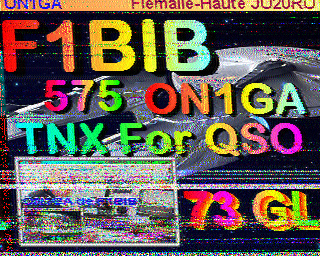
\includegraphics[width=0.85\textwidth]{foto/84}
    \caption{\scriptsize Ein per SSTV übertragenenes Bild}
    \label{n_sstv}
\end{figure}
\end{frame}

\begin{frame}
\only<1>{
\begin{QQuestion}{BE210}{Wie teilen Sie Ihrem Funkpartner in SSTV seinen \glqq Rapport\grqq{} mit?}{Ich teile ihm den Rapport später auf der QSL-Karte mit.}
{Ich schreibe den Rapport direkt in das zu übertragende Bild.}
{Ich sende den Rapport nach der Bildübertragung in CW.}
{Ich teile ihm den Rapport während der Bildübertragung in SSB mit.}
\end{QQuestion}

}
\only<2>{
\begin{QQuestion}{BE210}{Wie teilen Sie Ihrem Funkpartner in SSTV seinen \glqq Rapport\grqq{} mit?}{Ich teile ihm den Rapport später auf der QSL-Karte mit.}
{\textbf{\textcolor{DARCgreen}{Ich schreibe den Rapport direkt in das zu übertragende Bild.}}}
{Ich sende den Rapport nach der Bildübertragung in CW.}
{Ich teile ihm den Rapport während der Bildübertragung in SSB mit.}
\end{QQuestion}

}
\end{frame}%ENDCONTENT


\section{Notfunk}
\label{section:notfunk}
\begin{frame}%STARTCONTENT

\frametitle{Dürfen Funkamateure helfen?}
\begin{itemize}
  \item Ja! Funkamateure dürfen in Not- und Katastrophenfällen durch Übermittlung von Nachrichten für und an Dritte bei der Bewältigung einer Notlage unterstützen.
  \end{itemize}
\end{frame}

\begin{frame}
\only<1>{
\begin{QQuestion}{BF103}{Sie erreichen eine Unfallstelle. Der Ersthelfer bittet Sie, über Ihre mobile Amateurfunkstelle Hilfe zu holen, da das Mobiltelefonnetz nicht verfügbar ist. Wie verhalten Sie sich?}{Ich rufe per Funk einen Funkamateur und fordere diesen auf, die Polizei oder Rettungsleitstelle zu informieren.}
{Ich lehne es ab zu helfen, da im Amateurfunk keine Informationen für Dritte übermittelt werden dürfen.}
{Ich rufe per Funk mindestens dreimal MAYDAY gefolgt von meinem Rufzeichen, dem Standort und der Art der Notlage.}
{Ich lehne es ab zu helfen, da im Amateurfunk keine Notzeichen verwendet werden dürfen.}
\end{QQuestion}

}
\only<2>{
\begin{QQuestion}{BF103}{Sie erreichen eine Unfallstelle. Der Ersthelfer bittet Sie, über Ihre mobile Amateurfunkstelle Hilfe zu holen, da das Mobiltelefonnetz nicht verfügbar ist. Wie verhalten Sie sich?}{\textbf{\textcolor{DARCgreen}{Ich rufe per Funk einen Funkamateur und fordere diesen auf, die Polizei oder Rettungsleitstelle zu informieren.}}}
{Ich lehne es ab zu helfen, da im Amateurfunk keine Informationen für Dritte übermittelt werden dürfen.}
{Ich rufe per Funk mindestens dreimal MAYDAY gefolgt von meinem Rufzeichen, dem Standort und der Art der Notlage.}
{Ich lehne es ab zu helfen, da im Amateurfunk keine Notzeichen verwendet werden dürfen.}
\end{QQuestion}

}
\end{frame}

\begin{frame}
\frametitle{Was  tun, wenn man eine Notmeldung erhält?}
\begin{itemize}
  \item Bei einer Notmeldung sollte man zunächst aufmerksam zuhören und alle wichtigen Informationen notieren.
  \end{itemize}
\end{frame}

\begin{frame}
\only<1>{
\begin{QQuestion}{BF104}{Sie hören eine Notmeldung. Was tun Sie als Erstes?}{Ich wechsle die Frequenz oder schalte ab.}
{Ich sende dreimal MAYDAY, mein Rufzeichen und warte auf Antwort.}
{Ich stimme meinen Sender auf der Frequenz ab.}
{Ich höre aufmerksam zu und notiere alle wichtigen Informationen.}
\end{QQuestion}

}
\only<2>{
\begin{QQuestion}{BF104}{Sie hören eine Notmeldung. Was tun Sie als Erstes?}{Ich wechsle die Frequenz oder schalte ab.}
{Ich sende dreimal MAYDAY, mein Rufzeichen und warte auf Antwort.}
{Ich stimme meinen Sender auf der Frequenz ab.}
{\textbf{\textcolor{DARCgreen}{Ich höre aufmerksam zu und notiere alle wichtigen Informationen.}}}
\end{QQuestion}

}
\end{frame}

\begin{frame}
\frametitle{Was tun, wenn eine Rettungsorganisation sich der Sache annimmt?}
\begin{itemize}
  \item Wird die Notmeldung von einer Rettungsorganisation beantwortet, hält man sich zurück um den Funkbetrieb nicht zu stören.
  \end{itemize}
\end{frame}

\begin{frame}
\only<1>{
\begin{QQuestion}{BF105}{Sie haben eine Notmeldung aufgenommen, die nach kurzer Zeit von einer Rettungsorganisation beantwortet wird. Wie verhalten Sie sich?}{Ich bitte möglichst viele Funkamateure um Hilfe.}
{Ich biete zwischen zwei Durchgängen meine Hilfe an.}
{Ich stimme meinen Sender auf der Frequenz ab.}
{Ich störe auf keinen Fall den Funkbetrieb.}
\end{QQuestion}

}
\only<2>{
\begin{QQuestion}{BF105}{Sie haben eine Notmeldung aufgenommen, die nach kurzer Zeit von einer Rettungsorganisation beantwortet wird. Wie verhalten Sie sich?}{Ich bitte möglichst viele Funkamateure um Hilfe.}
{Ich biete zwischen zwei Durchgängen meine Hilfe an.}
{Ich stimme meinen Sender auf der Frequenz ab.}
{\textbf{\textcolor{DARCgreen}{Ich störe auf keinen Fall den Funkbetrieb.}}}
\end{QQuestion}

}
\end{frame}

\begin{frame}
\frametitle{Was tun, wenn zunächst niemand antwortet?}
\begin{itemize}
  \item Reagiert keine andere Funkstelle, beantwortet man den Ruf und informiert die Polizei oder Rettungsleitstelle.
  \end{itemize}
\end{frame}

\begin{frame}
\only<1>{
\begin{QQuestion}{BF106}{Sie haben eine Notmeldung aufgenommen. Keine andere Funkstelle reagiert und Sie könnten helfen. Wie verhalten Sie sich?}{Ich beantworte den Ruf und informiere die Polizei oder Rettungsleitstelle.}
{Ich schalte mein Funkgerät ab, um keine Probleme zu bekommen.}
{Ich wiederhole die Notmeldung umgehend auf derselben Frequenz.}
{Ich warte etwa eine Stunde, ob sich eine Rettungsorganisation meldet.}
\end{QQuestion}

}
\only<2>{
\begin{QQuestion}{BF106}{Sie haben eine Notmeldung aufgenommen. Keine andere Funkstelle reagiert und Sie könnten helfen. Wie verhalten Sie sich?}{\textbf{\textcolor{DARCgreen}{Ich beantworte den Ruf und informiere die Polizei oder Rettungsleitstelle.}}}
{Ich schalte mein Funkgerät ab, um keine Probleme zu bekommen.}
{Ich wiederhole die Notmeldung umgehend auf derselben Frequenz.}
{Ich warte etwa eine Stunde, ob sich eine Rettungsorganisation meldet.}
\end{QQuestion}

}
\end{frame}

\begin{frame}
\frametitle{Was tun, wenn man die zuständigen Stellen informiert hat?}
\begin{itemize}
  \item Idealerweise bleibt man erreichbar und gibt Informationen weiter, bis Hilfe eingetroffen ist.
  \end{itemize}
\end{frame}

\begin{frame}
\only<1>{
\begin{QQuestion}{BF107}{Sie haben eine Notmeldung beantwortet und die Polizei oder Rettungsleitstelle informiert. Welches Verhalten ist im Anschluss vorbildlich?}{Ich rufe regelmäßig die Polizei oder Rettungsleitstelle an und erkundige mich nach dem Stand.}
{Ich bleibe erreichbar und gebe Informationen weiter, bis Hilfe eingetroffen ist.}
{Ich schalte mein Funkgerät ab, da ich meiner Pflicht nachgekommen bin.}
{Ich informiere die Medien, damit über den Rettungseinsatz live berichtet werden kann.}
\end{QQuestion}

}
\only<2>{
\begin{QQuestion}{BF107}{Sie haben eine Notmeldung beantwortet und die Polizei oder Rettungsleitstelle informiert. Welches Verhalten ist im Anschluss vorbildlich?}{Ich rufe regelmäßig die Polizei oder Rettungsleitstelle an und erkundige mich nach dem Stand.}
{\textbf{\textcolor{DARCgreen}{Ich bleibe erreichbar und gebe Informationen weiter, bis Hilfe eingetroffen ist.}}}
{Ich schalte mein Funkgerät ab, da ich meiner Pflicht nachgekommen bin.}
{Ich informiere die Medien, damit über den Rettungseinsatz live berichtet werden kann.}
\end{QQuestion}

}
\end{frame}

\begin{frame}
\frametitle{Was ist bei internationaler Beteiligung zu beachten?}
\begin{itemize}
  \item Bei internationaler Beteiligung nutzt man UTC anstelle von lokaler Zeit.
  \end{itemize}
\end{frame}

\begin{frame}
\only<1>{
\begin{QQuestion}{BF108}{Sie haben am 16. August (Ortsdatum) um 20:00 Uhr mitteleuropäischer Sommerzeit (MESZ) von 9J2NG eine Notfunkmeldung aufgenommen und an eine Hilfeleistungsorganisation per Telefon weitergemeldet. Die Amateurfunkstelle 9J2NG hat Sie gebeten, um 23:00 Uhr UTC erneut mit ihr in Verbindung zu treten. Welcher Zeitpunkt ist dies in Deutschland?}{22:00 MESZ am 16. August (Ortsdatum)}
{21:00 MESZ am 16. August (Ortsdatum)}
{01:00 MESZ am 17. August (Ortsdatum)}
{00:00 MESZ am 18. August (Ortsdatum)}
\end{QQuestion}

}
\only<2>{
\begin{QQuestion}{BF108}{Sie haben am 16. August (Ortsdatum) um 20:00 Uhr mitteleuropäischer Sommerzeit (MESZ) von 9J2NG eine Notfunkmeldung aufgenommen und an eine Hilfeleistungsorganisation per Telefon weitergemeldet. Die Amateurfunkstelle 9J2NG hat Sie gebeten, um 23:00 Uhr UTC erneut mit ihr in Verbindung zu treten. Welcher Zeitpunkt ist dies in Deutschland?}{22:00 MESZ am 16. August (Ortsdatum)}
{21:00 MESZ am 16. August (Ortsdatum)}
{\textbf{\textcolor{DARCgreen}{01:00 MESZ am 17. August (Ortsdatum)}}}
{00:00 MESZ am 18. August (Ortsdatum)}
\end{QQuestion}

}
\end{frame}

\begin{frame}
\frametitle{Notzeichen}
\begin{itemize}
  \item Die Notzeichen außerhalb des Amateurfunks sind SOS und Mayday, diese dürfen im Amateurfunk nicht verwendet werden.
  \end{itemize}

\end{frame}

\begin{frame}
\only<1>{
\begin{QQuestion}{VD105}{Dürfen im Amateurfunkverkehr internationale Not-, Dringlichkeits- und Sicherheitszeichen (z. B. MAYDAY, PAN PAN, SÉCURITÉ) ausgesendet werden?}{Der Gebrauch dieser Zeichen ist auf den Kurzwellenbändern erlaubt.}
{Amateurfunkstellen in Küstennähe ist es erlaubt, diese Zeichen auszusenden.}
{Bei einem Notfall dürfen die Zeichen ausgesendet werden.}
{Der Gebrauch dieser Zeichen ist ausdrücklich untersagt.}
\end{QQuestion}

}
\only<2>{
\begin{QQuestion}{VD105}{Dürfen im Amateurfunkverkehr internationale Not-, Dringlichkeits- und Sicherheitszeichen (z. B. MAYDAY, PAN PAN, SÉCURITÉ) ausgesendet werden?}{Der Gebrauch dieser Zeichen ist auf den Kurzwellenbändern erlaubt.}
{Amateurfunkstellen in Küstennähe ist es erlaubt, diese Zeichen auszusenden.}
{Bei einem Notfall dürfen die Zeichen ausgesendet werden.}
{\textbf{\textcolor{DARCgreen}{Der Gebrauch dieser Zeichen ist ausdrücklich untersagt.}}}
\end{QQuestion}

}
\end{frame}

\begin{frame}
\only<1>{
\begin{QQuestion}{BF101}{Wie heißen die internationalen Notzeichen außerhalb des Amateurfunks?}{Prudence und TTT}
{Securité und Distresse}
{Distresse und DDD}
{Mayday und SOS}
\end{QQuestion}

}
\only<2>{
\begin{QQuestion}{BF101}{Wie heißen die internationalen Notzeichen außerhalb des Amateurfunks?}{Prudence und TTT}
{Securité und Distresse}
{Distresse und DDD}
{\textbf{\textcolor{DARCgreen}{Mayday und SOS}}}
\end{QQuestion}

}
\end{frame}

\begin{frame}
\only<1>{
\begin{QQuestion}{BF102}{Dürfen Sie im Notfall SOS oder Mayday innerhalb des Amateurfunks gebrauchen?}{SOS nicht, aber Mayday im Notfall.}
{Mayday nicht, aber SOS im Notfall.}
{Ja}
{Nein}
\end{QQuestion}

}
\only<2>{
\begin{QQuestion}{BF102}{Dürfen Sie im Notfall SOS oder Mayday innerhalb des Amateurfunks gebrauchen?}{SOS nicht, aber Mayday im Notfall.}
{Mayday nicht, aber SOS im Notfall.}
{Ja}
{\textbf{\textcolor{DARCgreen}{Nein}}}
\end{QQuestion}

}
\end{frame}

\begin{frame}
\frametitle{ Notfunkfrequenzen}
Die IARU hat für die ITU-Region 1 die folgenden Notfunkfrequenzen in den Bandplänen festgelegt, die für den Notfunkbetrieb frei zu halten sind:

\begin{itemize}
  \item 3.\qty{760}{\kilo\hertz}
  \item 7.\qty{110}{\kilo\hertz}
  \item 14.\qty{300}{\kilo\hertz}
  \item 18.\qty{160}{\kilo\hertz}
  \item 21.\qty{360}{\kilo\hertz}
  \end{itemize}
\end{frame}%ENDCONTENT


\title{DARC Amateurfunklehrgang Klasse N}
\author{Spannungsversorgung}
\institute{Deutscher Amateur Radio Club e.\,V.}
\begin{frame}
\maketitle
\end{frame}

\section{Elektrische Spannung}
\label{section:spannung}
\begin{frame}%STARTCONTENT
Wiederholung vom Anfang des Kurses:

\begin{itemize}
  \item Nach Trennung von positiven und negativen Ladungen versuchen diese wieder zusammenzukommen
  \item Es liegt eine elektrische Spannung vor
  \item Die Einheit ist Volt, abgekürzt V
  \end{itemize}
\end{frame}

\begin{frame}
\only<1>{
\begin{QQuestion}{NA201}{Welche Einheit wird üblicherweise für die elektrische Spannung verwendet?}{Ohm ($\Omega$)}
{Ampere (A)}
{Volt (V)}
{Amperestunden (Ah)}
\end{QQuestion}

}
\only<2>{
\begin{QQuestion}{NA201}{Welche Einheit wird üblicherweise für die elektrische Spannung verwendet?}{Ohm ($\Omega$)}
{Ampere (A)}
{\textbf{\textcolor{DARCgreen}{Volt (V)}}}
{Amperestunden (Ah)}
\end{QQuestion}

}
\end{frame}

\begin{frame}
\frametitle{Kleine Spannungen}
\begin{columns}
    \begin{column}{0.48\textwidth}
    \begin{itemize}
  \item Empfängereingang: 10 µV
  \item Mikrofon: 200 mV
  \item Batterie: 1,5 V oder 9 V
  \end{itemize}

    \end{column}
   \begin{column}{0.48\textwidth}
       \begin{table}
\begin{DARCtabular}{lrl}
     Bezeichnung  & Abkürzung  & Wert   \\
     1 Mikrovolt  & \qty{1}{\micro\volt}  & \qty{0,000001}{\volt}   \\
     1 Millivolt  & \qty{1}{\milli\volt}  & \qty{0,001}{\volt}   \\
     1 Volt  & \qty{1}{\volt}  & \qty{1}{\volt}   \\
\end{DARCtabular}
\caption{Kurzschreibweisen für kleine Spannungen}
\label{spannung_einheitenvorzeichen}
\end{table}

   \end{column}
\end{columns}

\end{frame}

\begin{frame}
\frametitle{Große Spannungen}
\begin{columns}
    \begin{column}{0.48\textwidth}
    \begin{itemize}
  \item Steckdose: 230 V
  \item Elektrostatisch aufgeladene Antenne: 1,5 kV
  \item Höchstspannungsleitung: 380 kV
  \end{itemize}

    \end{column}
   \begin{column}{0.48\textwidth}
       \begin{table}
\begin{DARCtabular}{lrr}
     Bezeichnung  & Abk.  & Wert   \\
     1 Kilovolt  & \qty{1}{\kilo\volt}  & \qty{1000}{\volt}   \\
     1 Megavolt  & \qty{1}{\mega\volt}  & \qty{1000000}{\volt}   \\
     1 Gigavolt  & \qty{1}{\giga\volt}  & \qty{1000000000}{\volt}   \\
\end{DARCtabular}
\caption{Kurzschreibweise für große Spannungen}
\label{n_frequenz_einheitenvorzeichen}
\end{table}

   \end{column}
\end{columns}

\end{frame}

\begin{frame}
\only<1>{
\begin{QQuestion}{NA208}{\qty{4,2}{\V} entspricht ...}{\qty{4,200}{\micro\volt}}
{\qty{4200}{\mV}}
{\qty{4200}{\kV}}
{\qty{4200}{\mega\V}}
\end{QQuestion}

}
\only<2>{
\begin{QQuestion}{NA208}{\qty{4,2}{\V} entspricht ...}{\qty{4,200}{\micro\volt}}
{\textbf{\textcolor{DARCgreen}{\qty{4200}{\mV}}}}
{\qty{4200}{\kV}}
{\qty{4200}{\mega\V}}
\end{QQuestion}

}
\end{frame}%ENDCONTENT


\section{Elektrischer Strom}
\label{section:strom}
\begin{frame}%STARTCONTENT

\frametitle{Stromkreis}
\begin{itemize}
  \item Beim Anschluss eines elektrischen Verbrauchers an die Pole einer Spannungsquelle, fangen die Ladungen an sich zu bewegen
  \item Das ist ein \emph{geschlossener Stromkreis}
  \item Je nach Spannung und Verbraucher fließt mehr oder weniger Strom
  \item Die \emph{elektrische Stromstärke} wird in Ampere (A) gemessen
  \end{itemize}
\end{frame}

\begin{frame}
\only<1>{
\begin{QQuestion}{NA202}{Welche Einheit wird üblicherweise für die elektrische Stromstärke verwendet?}{Amperestunden (Ah)}
{Volt (V)}
{Ohm ($\Omega$)}
{Ampere (A)}
\end{QQuestion}

}
\only<2>{
\begin{QQuestion}{NA202}{Welche Einheit wird üblicherweise für die elektrische Stromstärke verwendet?}{Amperestunden (Ah)}
{Volt (V)}
{Ohm ($\Omega$)}
{\textbf{\textcolor{DARCgreen}{Ampere (A)}}}
\end{QQuestion}

}
\end{frame}

\begin{frame}
\frametitle{Beispiele für Stromstärke}
\begin{table}
\begin{DARCtabular}{lrcl}
     Verbraucher  & & &  \\
     Leuchtdiode (LED)  & \qty{5}{\milli\ampere}  & =  & \qty{0,005}{\ampere}   \\
     Transceiver im Empfangsbetrieb  & \qty{900}{\milli\ampere}  & =  & \qty{0,9}{\ampere}   \\
     Transceiver im Sendebetrieb  & \qty{21}{\ampere}  & =  & \qty{21}{\ampere}   \\
\end{DARCtabular}
\caption{Beispiele für Ströme}
\label{strom_beispiele}
\end{table}
\end{frame}

\begin{frame}
\only<1>{
\begin{QQuestion}{NA209}{\qty{42}{\mA} entspricht~...}{\qty{0,42}{\A}.}
{\qty{0,0042}{\A}.}
{\qty{4,2}{\A}.}
{\qty{0,042}{\A}.}
\end{QQuestion}

}
\only<2>{
\begin{QQuestion}{NA209}{\qty{42}{\mA} entspricht~...}{\qty{0,42}{\A}.}
{\qty{0,0042}{\A}.}
{\qty{4,2}{\A}.}
{\textbf{\textcolor{DARCgreen}{\qty{0,042}{\A}.}}}
\end{QQuestion}

}
\end{frame}%ENDCONTENT


\section{Gefahren durch elektrischen Strom}
\label{section:gefahren}
\begin{frame}%STARTCONTENT
\begin{itemize}
  \item Stromschlag vermeiden!
  \item An anerkannte Regeln der Technik halten
  \item Vom Verband der Elektrotechnik Elektronik und Informationstechnik e.V. (VDE)
  \item Schutz von Menschen, Tieren und Sachen
  \end{itemize}
\end{frame}

\begin{frame}
\only<1>{
\begin{QQuestion}{VE601}{Wie ist die Stromversorgung von Eigenbaugeräten elektrotechnisch sicher aufzubauen?}{Es gelten die Vorschriften der örtlichen Stromversorger.}
{Es gelten keine besonderen Vorschriften, da ein Funkamateur eine sachkundige Person ist.}
{Nach den anerkannte Regeln der Technik, wie sie z. B. in den VDE-Normen festgelegt sind.}
{Sie ist nach den CEPT-Empfehlungen aufzubauen.}
\end{QQuestion}

}
\only<2>{
\begin{QQuestion}{VE601}{Wie ist die Stromversorgung von Eigenbaugeräten elektrotechnisch sicher aufzubauen?}{Es gelten die Vorschriften der örtlichen Stromversorger.}
{Es gelten keine besonderen Vorschriften, da ein Funkamateur eine sachkundige Person ist.}
{\textbf{\textcolor{DARCgreen}{Nach den anerkannte Regeln der Technik, wie sie z. B. in den VDE-Normen festgelegt sind.}}}
{Sie ist nach den CEPT-Empfehlungen aufzubauen.}
\end{QQuestion}

}
\end{frame}

\begin{frame}
\frametitle{Gefährliche Spannung}
\begin{itemize}
  \item Wechselspannung (AC) über 50 V
  \item Gleichspannung (DC) über 120 V
  \item Darunter kommt es zu keinen lebensbedrohlichen Beeinträchtigungen des menschlichen Körpers
  \end{itemize}

\end{frame}

\begin{frame}
\only<1>{
\begin{QQuestion}{NK301}{Ab welcher Höhe kann das Berühren elektrischer Wechselspannung (AC) und elektrischer Gleichspannung (DC) für den erwachsenen Menschen lebensgefährlich sein?}{\qty{50}{\V} (AC), \qty{120}{\V} (DC)}
{\qty{20}{\V} (AC), \qty{60}{\V} (DC)}
{\qty{100}{\V} (AC), \qty{140}{\V} (DC)}
{\qty{75}{\V} (AC), \qty{150}{\V} (DC)}
\end{QQuestion}

}
\only<2>{
\begin{QQuestion}{NK301}{Ab welcher Höhe kann das Berühren elektrischer Wechselspannung (AC) und elektrischer Gleichspannung (DC) für den erwachsenen Menschen lebensgefährlich sein?}{\textbf{\textcolor{DARCgreen}{\qty{50}{\V} (AC), \qty{120}{\V} (DC)}}}
{\qty{20}{\V} (AC), \qty{60}{\V} (DC)}
{\qty{100}{\V} (AC), \qty{140}{\V} (DC)}
{\qty{75}{\V} (AC), \qty{150}{\V} (DC)}
\end{QQuestion}

}
\end{frame}

\begin{frame}
\frametitle{Stromunfälle}
\begin{columns}
    \begin{column}{0.48\textwidth}
    \begin{itemize}
  \item Abhängig von Stromstärke und Dauer des Stromflusses
  \item Weg durch den Körper
  \item Ab 30 mA lebensgefährliche Schäden
  \end{itemize}

    \end{column}
   \begin{column}{0.48\textwidth}
       
\begin{figure}
    \DARCimage{0.85\linewidth}{681include}
    \caption{\scriptsize Stromschlag / Körperdurchströmung}
    \label{n_fehlerstrom}
\end{figure}


   \end{column}
\end{columns}

\end{frame}

\begin{frame}
\frametitle{Auswirkungen auf den Körper}
\begin{itemize}
  \item \emph{Herzrhythmusstörungen}, Herzkammerflimmern oder Herzstillstand, inbesondere bei einem Stromweg im Brustbereich
  \item \emph{Verbrennungen}, meist an den Ein- und Austrittstellen des elektrischen Stroms
  \item \emph{Verkrampfen der Muskulatur}
  \item \emph{Sekundärunfälle} wie einen Sturz, verursacht durch den hervorgerufenden Schreck oder eine Muskelverkrampfung
  \item Zusätzlich \emph{(Stör-)Lichtbogen} mit hellem Leuchten über die Luft möglich
  \end{itemize}
\end{frame}

\begin{frame}
\frametitle{Gefahr beim Öffnen von Geräten}
\begin{itemize}
  \item Kondensatoren können hohe Spannungen speichern
  \item Es können in abgeschalteten Geräten noch gefährliche Spannungen anliegen
  \item Beim Öffnen von Geräten erfahrenen Funkamateur oder Elektrofachkraft zu Hilfe holen
  \end{itemize}
\end{frame}

\begin{frame}
\only<1>{
\begin{QQuestion}{NK303}{Welche gefährlichen Folgen kann eine Körperdurchströmung mit elektrischem Strom verursachen?}{Verätzungen, Muskelentzündungen, Herzklopfen}
{Verbrennungen, Muskelverkrampfungen, Herzrhythmusstörungen}
{Verbrühungen, Muskelkater, Atembeschwerden}
{Verkochungen, Muskelzucken, Herzasthma}
\end{QQuestion}

}
\only<2>{
\begin{QQuestion}{NK303}{Welche gefährlichen Folgen kann eine Körperdurchströmung mit elektrischem Strom verursachen?}{Verätzungen, Muskelentzündungen, Herzklopfen}
{\textbf{\textcolor{DARCgreen}{Verbrennungen, Muskelverkrampfungen, Herzrhythmusstörungen}}}
{Verbrühungen, Muskelkater, Atembeschwerden}
{Verkochungen, Muskelzucken, Herzasthma}
\end{QQuestion}

}
\end{frame}

\begin{frame}
\only<1>{
\begin{QQuestion}{NK302}{Die größten Gefährdungen durch elektrischen Strom sind insbesondere~...}{Lichtblitze, Stromspitzen, Folgeschäden durch Ohnmacht}
{Stromschlag, Kurzschluss, Auslösen von Sicherungen}
{Stromunfälle, Spannungsabfälle, Unfälle durch Erschrecken}
{elektrische Körperdurchströmung, Störlichtbogen, Sekundärunfälle}
\end{QQuestion}

}
\only<2>{
\begin{QQuestion}{NK302}{Die größten Gefährdungen durch elektrischen Strom sind insbesondere~...}{Lichtblitze, Stromspitzen, Folgeschäden durch Ohnmacht}
{Stromschlag, Kurzschluss, Auslösen von Sicherungen}
{Stromunfälle, Spannungsabfälle, Unfälle durch Erschrecken}
{\textbf{\textcolor{DARCgreen}{elektrische Körperdurchströmung, Störlichtbogen, Sekundärunfälle}}}
\end{QQuestion}

}
\end{frame}

\begin{frame}
\frametitle{Erste Hilfe}
\begin{itemize}
  \item In den ersten Minuten entscheidend für die Schwere der Unfallfolgen
  \item Unbedingt Arzt aufsuchen
  \item Herzrhythmusstörungen und Herzkammerflimmern können Stunden nach dem Unfall auftreten
  \end{itemize}

\end{frame}

\begin{frame}
\only<1>{
\begin{QQuestion}{NK304}{Welche Maßnahme ist nach einem Elektrounfall mit Körperdurchströmung (Stromschlag) zu ergreifen?}{Es ist ein Arzt aufzusuchen, da Herzrhythmusstörungen und Herzkammerflimmern auch noch viele Stunden nach einem Stromschlag auftreten können.}
{Personen, die einen Stromschlag erlitten haben, sind unverzüglich in eine stabile Seitenlage zu bringen.}
{Sofern sich die verunfallte Person gut fühlt, sind keine Maßnahmen erforderlich.}
{Bei Stromschlag mit Wechselstrom (AC) ist ein Arzt aufzusuchen, bei Stromschlag mit Gleichstrom (DC) ist kein Arzt erforderlich.}
\end{QQuestion}

}
\only<2>{
\begin{QQuestion}{NK304}{Welche Maßnahme ist nach einem Elektrounfall mit Körperdurchströmung (Stromschlag) zu ergreifen?}{\textbf{\textcolor{DARCgreen}{Es ist ein Arzt aufzusuchen, da Herzrhythmusstörungen und Herzkammerflimmern auch noch viele Stunden nach einem Stromschlag auftreten können.}}}
{Personen, die einen Stromschlag erlitten haben, sind unverzüglich in eine stabile Seitenlage zu bringen.}
{Sofern sich die verunfallte Person gut fühlt, sind keine Maßnahmen erforderlich.}
{Bei Stromschlag mit Wechselstrom (AC) ist ein Arzt aufzusuchen, bei Stromschlag mit Gleichstrom (DC) ist kein Arzt erforderlich.}
\end{QQuestion}

}
\end{frame}

\begin{frame}
\frametitle{5 Sicherheitsregeln in der Elektrotechnik}
\begin{enumerate}
  \item[1] \emph{Freischalten}, z.\,B. Gerät ausschalten
  \item[2] \emph{Gegen Wiedereinschalten sichern}, z.\,B.  Stecker ziehen
  \item[3] \emph{Spannungsfreiheit feststellen}, z.\,B. mit einem Multimeter messen
  \item[4] \emph{Erden und Kurzschließen}, z.\,B. das Gehäuse und Zuleitungen erden
  \item[5] \emph{Benachbarte, unter Spannung stehende Teile abdecken oder abschranken} (findet bei einzelnen Geräten meist keine Anwendung)
  \end{enumerate}
\end{frame}%ENDCONTENT


\section{Netzgerät}
\label{section:netzgeraet_1}
\begin{frame}%STARTCONTENT

\begin{columns}
    \begin{column}{0.48\textwidth}
    \begin{itemize}
  \item Netzgerät wandelt Wechselspannung von 230 V aus der Steckdose in kleinere Gleichspannung um
  \item Im Amateurfunk wird häufig 13,8 V für Transceiver verwendet
  \end{itemize}

    \end{column}
   \begin{column}{0.48\textwidth}
       
\begin{figure}
    \DARCimage{0.85\linewidth}{740include}
    \caption{\scriptsize Netzgerät}
    \label{n_netzgeraet}
\end{figure}


   \end{column}
\end{columns}

\end{frame}

\begin{frame}
\only<1>{
\begin{QQuestion}{ND101}{Ein Mobilfunktransceiver ist an ein Netzgerät angeschlossen. Welche Aufgabe hat das Netzgerät?}{Die Stabilisierung der \qty{230}{\V} Wechselspannung.}
{Erzeugung einer Wechselspannung aus einer Gleichspannung.}
{Erzeugung einer Gleichspannung aus dem \qty{230}{\V} Wechselspannungsnetz.}
{Eine Internetverbindung zum Funkgerät herzustellen.}
\end{QQuestion}

}
\only<2>{
\begin{QQuestion}{ND101}{Ein Mobilfunktransceiver ist an ein Netzgerät angeschlossen. Welche Aufgabe hat das Netzgerät?}{Die Stabilisierung der \qty{230}{\V} Wechselspannung.}
{Erzeugung einer Wechselspannung aus einer Gleichspannung.}
{\textbf{\textcolor{DARCgreen}{Erzeugung einer Gleichspannung aus dem \qty{230}{\V} Wechselspannungsnetz.}}}
{Eine Internetverbindung zum Funkgerät herzustellen.}
\end{QQuestion}

}
\end{frame}

\begin{frame}
\only<1>{
\begin{QQuestion}{ND102}{Welche Spannung liefert ein Netzgerät für einen Mobilfunk-Transceiver üblicherweise?}{ca. \qty{13,8}{\V} Gleichspannung}
{ca. \qty{230}{\V} Gleichspannung}
{ca. \qty{13,8}{\V} Wechselspannung}
{ca. \qty{230}{\V} Wechselspannung}
\end{QQuestion}

}
\only<2>{
\begin{QQuestion}{ND102}{Welche Spannung liefert ein Netzgerät für einen Mobilfunk-Transceiver üblicherweise?}{\textbf{\textcolor{DARCgreen}{ca. \qty{13,8}{\V} Gleichspannung}}}
{ca. \qty{230}{\V} Gleichspannung}
{ca. \qty{13,8}{\V} Wechselspannung}
{ca. \qty{230}{\V} Wechselspannung}
\end{QQuestion}

}
\end{frame}

\begin{frame}
\frametitle{Schutzkontakt}
\begin{columns}
    \begin{column}{0.48\textwidth}
    \begin{itemize}
  \item Beim \emph{Schutzkontaktstecker} gibt es drei Pole
  \item L- und N-Leiter durch Stifte
  \item Dort liegt die 230 V-Spanung an
  \item \emph{Schutzkontakt} ist der dritte Pol
  \item PE-Leiter durch äußere Schleifkontakte
  \end{itemize}

    \end{column}
   \begin{column}{0.48\textwidth}
       
\begin{figure}
    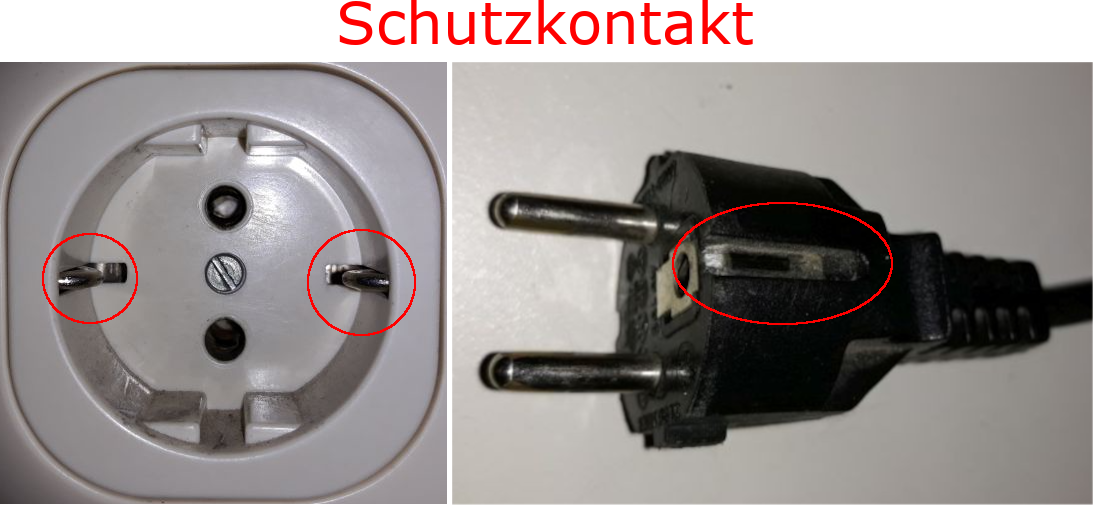
\includegraphics[width=0.85\textwidth]{foto/86}
    \caption{\scriptsize Schutzkontakt an einer Steckdose und Schukostecker}
    \label{n_schutzkontakt}
\end{figure}

   \end{column}
\end{columns}

\end{frame}

\begin{frame}
\only<1>{
\begin{QQuestion}{ND109}{Welche Verbindung stellt der Schutzkontakt in einem Schutzkontakt-Stecker (Schuko-Stecker) her?}{Verbindung zum L-Leiter der Steckdose}
{Verbindung zwischen PE- und N-Leiter in der Steckdose}
{Verbindung zum N-Leiter der Steckdose}
{Verbindung zum PE-Leiter der Steckdose}
\end{QQuestion}

}
\only<2>{
\begin{QQuestion}{ND109}{Welche Verbindung stellt der Schutzkontakt in einem Schutzkontakt-Stecker (Schuko-Stecker) her?}{Verbindung zum L-Leiter der Steckdose}
{Verbindung zwischen PE- und N-Leiter in der Steckdose}
{Verbindung zum N-Leiter der Steckdose}
{\textbf{\textcolor{DARCgreen}{Verbindung zum PE-Leiter der Steckdose}}}
\end{QQuestion}

}
\end{frame}

\begin{frame}
\frametitle{Gleichspannungsausgang}

\begin{figure}
    \DARCimage{0.85\linewidth}{680include}
    \caption{\scriptsize Anschluss von Netzgerät und TRX}
    \label{n_Netzgeraet_TRX}
\end{figure}
\begin{columns}
    \begin{column}{0.48\textwidth}
    \begin{itemize}
  \item Ist zweipolig zum Transceiver
  \item Klemmen sind in der Regel farbig
  \end{itemize}

    \end{column}
   \begin{column}{0.48\textwidth}
       
    \pause
    \begin{itemize}
  \item Rot für Plus
  \item Schwarz für Minus
  \item Polung beachten!
  \end{itemize}



   \end{column}
\end{columns}

\end{frame}

\begin{frame}
\only<1>{
\begin{QQuestion}{ND104}{Warum ist die Spannungsversorgungsleitung vom externen Netzteil zum Transceiver zweipolig ausgeführt?}{Damit die Spannungsreduzierung nicht zu hoch wird.}
{Damit von beiden Polen des Netzteils der Strom zum Transceiver fließen kann.}
{Der Transceiver nutzt eine Leitung, die andere Leitung dient zur Erdung.
}
{Damit der Stromkreis über den Transceiver geschlossen werden kann.}
\end{QQuestion}

}
\only<2>{
\begin{QQuestion}{ND104}{Warum ist die Spannungsversorgungsleitung vom externen Netzteil zum Transceiver zweipolig ausgeführt?}{Damit die Spannungsreduzierung nicht zu hoch wird.}
{Damit von beiden Polen des Netzteils der Strom zum Transceiver fließen kann.}
{Der Transceiver nutzt eine Leitung, die andere Leitung dient zur Erdung.
}
{\textbf{\textcolor{DARCgreen}{Damit der Stromkreis über den Transceiver geschlossen werden kann.}}}
\end{QQuestion}

}
\end{frame}

\begin{frame}
\only<1>{
\begin{QQuestion}{ND103}{Warum ist die Spannungsversorgungsleitung vom Gleichspannungsnetzteil zum Transceiver zweipolig ausgeführt?}{Der Strom fließt in beide Leiter hinein und über die Erde zum Netzteil zurück.}
{Der Strom fließt in einem Leiter hin und im anderen Leiter wieder zurück.}
{Damit insgesamt mehr Strom fließen kann.}
{Der Strom fließt aus beiden Leitern heraus und über die Erde zum Netzteil zurück.}
\end{QQuestion}

}
\only<2>{
\begin{QQuestion}{ND103}{Warum ist die Spannungsversorgungsleitung vom Gleichspannungsnetzteil zum Transceiver zweipolig ausgeführt?}{Der Strom fließt in beide Leiter hinein und über die Erde zum Netzteil zurück.}
{\textbf{\textcolor{DARCgreen}{Der Strom fließt in einem Leiter hin und im anderen Leiter wieder zurück.}}}
{Damit insgesamt mehr Strom fließen kann.}
{Der Strom fließt aus beiden Leitern heraus und über die Erde zum Netzteil zurück.}
\end{QQuestion}

}
\end{frame}

\begin{frame}
\only<1>{
\begin{QQuestion}{ND105}{Wie sind die Klemmen einer \qty{13,8}{\V} Gleichspannungsversorgung gekennzeichnet?}{Pluspol schwarz, Minuspol grüngelb}
{Pluspol blau, Minuspol rot}
{Pluspol rot, Minuspol schwarz}
{Pluspol braun, Minuspol grüngelb}
\end{QQuestion}

}
\only<2>{
\begin{QQuestion}{ND105}{Wie sind die Klemmen einer \qty{13,8}{\V} Gleichspannungsversorgung gekennzeichnet?}{Pluspol schwarz, Minuspol grüngelb}
{Pluspol blau, Minuspol rot}
{\textbf{\textcolor{DARCgreen}{Pluspol rot, Minuspol schwarz}}}
{Pluspol braun, Minuspol grüngelb}
\end{QQuestion}

}
\end{frame}

\begin{frame}
\only<1>{
\begin{QQuestion}{ND106}{Worauf ist beim Anschluss eines Gleichspannungsnetzteils an einen Transceiver  besonders zu achten?}{Korrekte Verbindung zur Antenne}
{Richtige Polung des Schutzkontaktsteckers}
{Polungsrichtiger Anschluss der Stromversorgungsleitung zum Transceiver}
{Polungsrichtiger Anschluss des SWR-Meters}
\end{QQuestion}

}
\only<2>{
\begin{QQuestion}{ND106}{Worauf ist beim Anschluss eines Gleichspannungsnetzteils an einen Transceiver  besonders zu achten?}{Korrekte Verbindung zur Antenne}
{Richtige Polung des Schutzkontaktsteckers}
{\textbf{\textcolor{DARCgreen}{Polungsrichtiger Anschluss der Stromversorgungsleitung zum Transceiver}}}
{Polungsrichtiger Anschluss des SWR-Meters}
\end{QQuestion}

}
\end{frame}

\begin{frame}
\only<1>{
\begin{QQuestion}{ND107}{Welche Folge kann eine Verpolung der Leitung vom Netzteil zum Transceiver nach sich ziehen?}{Ausfall der Backup-Batterie im Transceiver}
{Verzerrung des Sendesignals}
{Beschädigung des Funkgeräts}
{Verzerrung des Empfangssignals}
\end{QQuestion}

}
\only<2>{
\begin{QQuestion}{ND107}{Welche Folge kann eine Verpolung der Leitung vom Netzteil zum Transceiver nach sich ziehen?}{Ausfall der Backup-Batterie im Transceiver}
{Verzerrung des Sendesignals}
{\textbf{\textcolor{DARCgreen}{Beschädigung des Funkgeräts}}}
{Verzerrung des Empfangssignals}
\end{QQuestion}

}
\end{frame}

\begin{frame}
\frametitle{Feinsicherungen}
\begin{columns}
    \begin{column}{0.48\textwidth}
    
\begin{figure}
    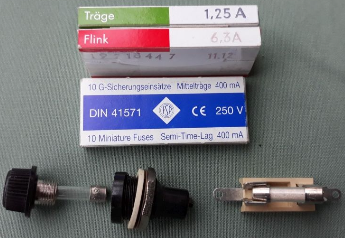
\includegraphics[width=0.85\textwidth]{foto/88}
    \caption{\scriptsize Feinsicherungen}
    \label{n_feinsicherungen}
\end{figure}

    \end{column}
   \begin{column}{0.48\textwidth}
       \begin{itemize}
  \item Unterbrechen Stromfluss im Fehlerfall (Kurzschluss oder Überlastung)
  \item Schmelzsicherungen in denen ein dünner Draht schmilzt
  \item \emph{Durchgebrannte Sicherung} bzw. \emph{thermische Abschaltung}
  \end{itemize}

   \end{column}
\end{columns}

\end{frame}

\begin{frame}
\frametitle{Feinsicherungen austauschen}
\begin{itemize}
  \item Erst die Ursache beheben
  \item Durch gleichartige ersetzen
  \item Stromstärke und Auslösecharakteristik
  \end{itemize}
\end{frame}

\begin{frame}
\frametitle{Kenngrößen von Feinsicherungen}
\begin{table}
\begin{DARCtabular}{ccc}
     Auslösecharakteristik  & Kennzeichen  & Abschaltzeit bei zehnfachem Nennstrom   \\
     flink  & F  & max. 30 ms  \\
     mittelträge  & MT  & max. 90 ms   \\
     träge  & T  & max. 300 ms   \\
\end{DARCtabular}
\caption{Kenngrößen von Feinsicherungen}
\label{n_feinsicherung}
\end{table}
\end{frame}

\begin{frame}
\frametitle{Elektronische Begrenzung}
\begin{itemize}
  \item In hochwertigen Netzgeräten
  \item Im Kurzschlussfall wird die Stromstärke begrenzt
  \item \emph{Kurzschlussstrombegrenzung}
  \item Kein Austausch von Sicherungen notwendig
  \end{itemize}
\end{frame}%ENDCONTENT


\section{Batterien und Akkus}
\label{section:batterien_und_akkus}
\begin{frame}%STARTCONTENT

\begin{columns}
    \begin{column}{0.48\textwidth}
    \begin{itemize}
  \item Spannung durch Ladungstrennung in elektrochemischen Vorgängen
  \item Beim Akku ist der Vorgang umkehrbar
  \item Plus- oder Minuspol gekennzeichnet
  \end{itemize}

    \end{column}
   \begin{column}{0.48\textwidth}
       
\begin{figure}
    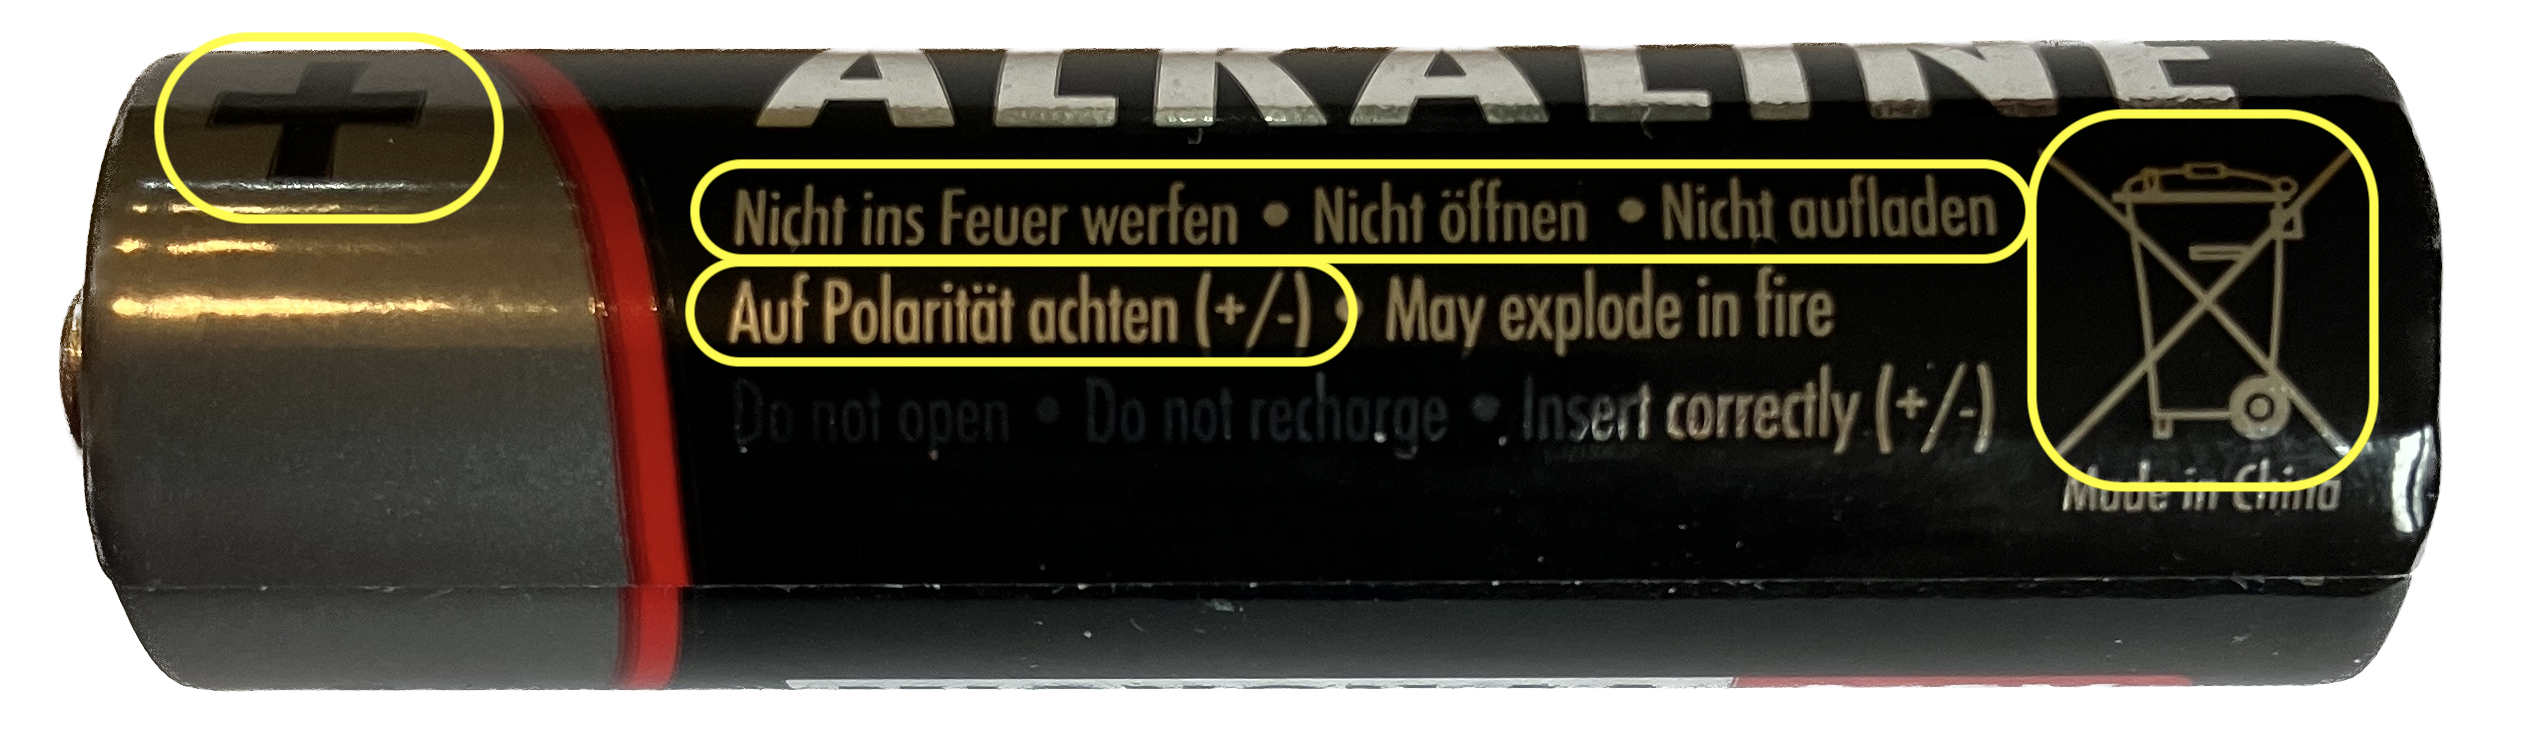
\includegraphics[width=0.85\textwidth]{foto/89}
    \caption{\scriptsize Eine Batterie mit Kennzeichnung der Pole und Warnhinweisen}
    \label{n_Bat_AA}
\end{figure}

\begin{figure}
    \DARCimage{0.85\linewidth}{517include}
    \caption{\scriptsize Schaltzeichen einer Batterie}
    \label{n_schaltzeichen_batt}
\end{figure}


   \end{column}
\end{columns}

\end{frame}

\begin{frame}
\only<1>{
\begin{PQuestion}{NB201}{Welches Bauteil wird durch das Schaltzeichen symbolisiert?}{Batterie}
{Diode}
{Widerstand}
{Kondensator}
{\DARCimage{0.5\linewidth}{510include}}\end{PQuestion}

}
\only<2>{
\begin{PQuestion}{NB201}{Welches Bauteil wird durch das Schaltzeichen symbolisiert?}{\textbf{\textcolor{DARCgreen}{Batterie}}}
{Diode}
{Widerstand}
{Kondensator}
{\DARCimage{0.5\linewidth}{510include}}\end{PQuestion}

}
\end{frame}

\begin{frame}
\only<1>{
\begin{PQuestion}{NB203}{Wie lauten die Bezeichnungen für die Anschlüsse 1 und 2 im Schaltsymbol?}{1 = Nord-Pol; 2 = Süd-Pol}
{1 = Minus-Pol; 2 = Plus-Pol}
{1 = Plus-Pol; 2 = Minus-Pol}
{1 = Süd-Pol; 2 = Nord-Pol}
{\DARCimage{0.5\linewidth}{517include}}\end{PQuestion}

}
\only<2>{
\begin{PQuestion}{NB203}{Wie lauten die Bezeichnungen für die Anschlüsse 1 und 2 im Schaltsymbol?}{1 = Nord-Pol; 2 = Süd-Pol}
{1 = Minus-Pol; 2 = Plus-Pol}
{\textbf{\textcolor{DARCgreen}{1 = Plus-Pol; 2 = Minus-Pol}}}
{1 = Süd-Pol; 2 = Nord-Pol}
{\DARCimage{0.5\linewidth}{517include}}\end{PQuestion}

}
\end{frame}

\begin{frame}
\frametitle{Serienschaltung}
\begin{columns}
    \begin{column}{0.48\textwidth}
    \begin{itemize}
  \item Batterien lassen sich hintereinander schalten
  \item Pluspol auf Minuspol der vorhergehenden Batterie
  \item Die Gesamtspannung ist die Summe der Einzelspannungen
  \end{itemize}

    \end{column}
   \begin{column}{0.48\textwidth}
       
\begin{figure}
    \DARCimage{0.85\linewidth}{748include}
    \caption{\scriptsize Verschiedene Batterien und Akkus}
    \label{batterien_und_akkus_sammlung}
\end{figure}


   \end{column}
\end{columns}

\end{frame}

\begin{frame}
\only<1>{
\begin{PQuestion}{NB204}{Folgende Schaltung besteht aus Spannungsquellen von je \qty{1,5}{\V}. Welche Spannung misst man zwischen den Kontakten, die mit \glqq +\grqq{} und \glqq -\grqq{} gekennzeichnet sind?}{\qty{0,25}{\V}}
{\qty{1,5}{\V}}
{\qty{9}{\V}}
{\qty{6}{\V}}
{\DARCimage{1.0\linewidth}{431include}}\end{PQuestion}

}
\only<2>{
\begin{PQuestion}{NB204}{Folgende Schaltung besteht aus Spannungsquellen von je \qty{1,5}{\V}. Welche Spannung misst man zwischen den Kontakten, die mit \glqq +\grqq{} und \glqq -\grqq{} gekennzeichnet sind?}{\qty{0,25}{\V}}
{\qty{1,5}{\V}}
{\textbf{\textcolor{DARCgreen}{\qty{9}{\V}}}}
{\qty{6}{\V}}
{\DARCimage{1.0\linewidth}{431include}}\end{PQuestion}

}
\end{frame}

\begin{frame}
\frametitle{Kurzschluss}
\begin{itemize}
  \item Vermeiden!
  \item Bei Akkus Gefahr der Überhitzung
  \item Brandgefahr
  \end{itemize}
\end{frame}

\begin{frame}
\only<1>{
\begin{QQuestion}{ND110}{Was ist bei der Verwendung von Akkus und Batterien zu beachten?}{Sie müssen paarweise verwendet werden.}
{Ein Kurzschluss ist zu vermeiden.}
{Sie müssen mit einem Mindestentladestrom betrieben werden.}
{Sie sollen stets vollkommen entladen werden.}
\end{QQuestion}

}
\only<2>{
\begin{QQuestion}{ND110}{Was ist bei der Verwendung von Akkus und Batterien zu beachten?}{Sie müssen paarweise verwendet werden.}
{\textbf{\textcolor{DARCgreen}{Ein Kurzschluss ist zu vermeiden.}}}
{Sie müssen mit einem Mindestentladestrom betrieben werden.}
{Sie sollen stets vollkommen entladen werden.}
\end{QQuestion}

}
 \end{frame}

\begin{frame}
\frametitle{Unsachgemäßer Umgang}
\begin{itemize}
  \item In Akkus sind verschiedene chemische Technologien im Einsatz
  \item Beim Aufladen angepasste Ladegeräte verwenden
  \item Gefahr von Überhitzung, Explosion oder Brand
  \item Dadurch kann es zu Verbrennungen, Verätzungen und Vergiftungen kommen
  \end{itemize}
\end{frame}

\begin{frame}
\only<1>{
\begin{QQuestion}{NK306}{Welche Gefahren drohen dem Anwender bei unsachgemäßem Umgang mit wiederaufladbaren Batterien?}{Verätzungen, Spannungsschwankungen, Ruhestromanstieg}
{Überstrom, Unterspannung, Leistungsreduzierung}
{Verbrennungen, Verätzungen, Vergiftungen}
{Anstieg des Innenwiderstands, Spannungsschwankungen, Leistungsreduzierung}
\end{QQuestion}

}
\only<2>{
\begin{QQuestion}{NK306}{Welche Gefahren drohen dem Anwender bei unsachgemäßem Umgang mit wiederaufladbaren Batterien?}{Verätzungen, Spannungsschwankungen, Ruhestromanstieg}
{Überstrom, Unterspannung, Leistungsreduzierung}
{\textbf{\textcolor{DARCgreen}{Verbrennungen, Verätzungen, Vergiftungen}}}
{Anstieg des Innenwiderstands, Spannungsschwankungen, Leistungsreduzierung}
\end{QQuestion}

}
 \end{frame}%ENDCONTENT


\title{DARC Amateurfunklehrgang Klasse N}
\author{Bauteile und Schaltkreise}
\institute{Deutscher Amateur Radio Club e.\,V.}
\begin{frame}
\maketitle
\end{frame}

\section{Recht zum Selbstbau}
\label{section:recht_zum_selbstbau}
\begin{frame}%STARTCONTENT
\begin{itemize}
  \item Sender und Sendeanlagen benötigen normalerweise eine behördliche Zulassung
  \item Funkamateure sind davon ausgenommen
  \item Sie sind berechtigt, \emph{im Handel erhältliche, selbstgefertigte oder auf Amateurfunkfrequenzen umgebaute Sendeanlagen} zu betreiben
  \end{itemize}

\end{frame}

\begin{frame}
\only<1>{
\begin{QQuestion}{VC109}{Welches Recht haben Funkamateure in Bezug auf den Betrieb von Sendeanlagen? Ein Funkamateur~...}{muss die einschlägigen Bestimmungen der BNetzA zur elektrischen Sicherheit nicht beachten.}
{benötigt in keinem Fall eine Standortbescheinigung der BNetzA für seine Amateurfunkstelle.}
{ist berechtigt, im Handel erhältliche, selbst gefertigte oder auf Amateurfunkfrequenzen umgebaute Sendeanlagen zu betreiben.}
{darf mit seiner Amateurfunkstelle jederzeit Nachrichten für und an Dritte übermitteln, die nicht den Amateurfunkdienst betreffen.}
\end{QQuestion}

}
\only<2>{
\begin{QQuestion}{VC109}{Welches Recht haben Funkamateure in Bezug auf den Betrieb von Sendeanlagen? Ein Funkamateur~...}{muss die einschlägigen Bestimmungen der BNetzA zur elektrischen Sicherheit nicht beachten.}
{benötigt in keinem Fall eine Standortbescheinigung der BNetzA für seine Amateurfunkstelle.}
{\textbf{\textcolor{DARCgreen}{ist berechtigt, im Handel erhältliche, selbst gefertigte oder auf Amateurfunkfrequenzen umgebaute Sendeanlagen zu betreiben.}}}
{darf mit seiner Amateurfunkstelle jederzeit Nachrichten für und an Dritte übermitteln, die nicht den Amateurfunkdienst betreffen.}
\end{QQuestion}

}
\end{frame}

\begin{frame}
\frametitle{Bauteile}
\begin{itemize}
  \item Zum Selbstbau werden verschiede elektronische Bauteile benötigt
  \item Diese weisen unterschiedliche Eigenschaften auf
  \item In Klasse~N gibt es nur wenige, einfache Schaltungen $\rightarrow$ mehr in Klasse~E und A
  \item Kenntnisse der Symbole und Bezeichnungen reichen
  \end{itemize}

\end{frame}

\begin{frame}
\frametitle{Anforderungen an Funkgeräte}
\begin{itemize}
  \item Alle \emph{im Handel erhältlichen, seriengefertigten Funkanlagen} müssen die \emph{grundlegenden Anforderungen und Bestimmungen des Funkanlagengesetzes (FuAG)} einhalten
  \item EU-Konformitätserklärung (\emph{CE-Kennzeichnung}) vor in Verkehr bringen erstellen
  \item Nur dann dürfen vom Markt bereitgestellte Anlagen in Betrieb genommen werden
  \end{itemize}

\end{frame}

\begin{frame}
\only<1>{
\begin{QQuestion}{VE401}{Welches Gesetz regelt unter anderem das Inverkehrbringen, den freien Warenverkehr und die Inbetriebnahme von auf dem Markt bereitgestellten Amateurfunkanlagen?}{Das Gesetz über die elektromagnetische Verträglichkeit von Betriebsmitteln (EMVG)}
{Die Amateurfunkverordnung (AfuV)}
{Das Funkanlagengesetz (FuAG)}
{Für solche Amateurfunkgeräte gibt es keine Regelung.}
\end{QQuestion}

}
\only<2>{
\begin{QQuestion}{VE401}{Welches Gesetz regelt unter anderem das Inverkehrbringen, den freien Warenverkehr und die Inbetriebnahme von auf dem Markt bereitgestellten Amateurfunkanlagen?}{Das Gesetz über die elektromagnetische Verträglichkeit von Betriebsmitteln (EMVG)}
{Die Amateurfunkverordnung (AfuV)}
{\textbf{\textcolor{DARCgreen}{Das Funkanlagengesetz (FuAG)}}}
{Für solche Amateurfunkgeräte gibt es keine Regelung.}
\end{QQuestion}

}
\end{frame}

\begin{frame}
\only<1>{
\begin{QQuestion}{VE402}{Welche Geräte fallen in den Anwendungsbereich des Funkanlagengesetzes (FuAG)?}{Selbstgebaute Amateurfunkanlagen}
{Auf dem Markt bereitgestellte Amateurfunkanlagen}
{Kommerziell hergestellte Funkanlagen, die zu Amateurfunkzwecken umgebaut wurden}
{Bausätze für Amateurfunkanlagen}
\end{QQuestion}

}
\only<2>{
\begin{QQuestion}{VE402}{Welche Geräte fallen in den Anwendungsbereich des Funkanlagengesetzes (FuAG)?}{Selbstgebaute Amateurfunkanlagen}
{\textbf{\textcolor{DARCgreen}{Auf dem Markt bereitgestellte Amateurfunkanlagen}}}
{Kommerziell hergestellte Funkanlagen, die zu Amateurfunkzwecken umgebaut wurden}
{Bausätze für Amateurfunkanlagen}
\end{QQuestion}

}
\end{frame}

\begin{frame}
\only<1>{
\begin{QQuestion}{VE403}{Welche grundlegenden Anforderungen werden nach dem Funkanlagengesetz (FuAG) an Amateurfunkgeräte gestellt?}{Die Funkgeräte müssen eine nationale Zulassungskennzeichnung nach Vorgabe der BNetzA tragen.}
{Seriengefertigte Geräte müssen die grundlegenden Anforderungen nach dem Funkanlagengesetz (FuAG) einhalten und eine CE-Kennzeichnung tragen.}
{Selbstgebaute Funkgeräte müssen die grundlegenden Anforderungen nach dem Funkanlagengesetz (FuAG) einhalten und eine CE-Kennzeichnung tragen.}
{Seriengefertigte Amateurfunkgeräte unterliegen nicht dem Funkanlagengesetz (FuAG).}
\end{QQuestion}

}
\only<2>{
\begin{QQuestion}{VE403}{Welche grundlegenden Anforderungen werden nach dem Funkanlagengesetz (FuAG) an Amateurfunkgeräte gestellt?}{Die Funkgeräte müssen eine nationale Zulassungskennzeichnung nach Vorgabe der BNetzA tragen.}
{\textbf{\textcolor{DARCgreen}{Seriengefertigte Geräte müssen die grundlegenden Anforderungen nach dem Funkanlagengesetz (FuAG) einhalten und eine CE-Kennzeichnung tragen.}}}
{Selbstgebaute Funkgeräte müssen die grundlegenden Anforderungen nach dem Funkanlagengesetz (FuAG) einhalten und eine CE-Kennzeichnung tragen.}
{Seriengefertigte Amateurfunkgeräte unterliegen nicht dem Funkanlagengesetz (FuAG).}
\end{QQuestion}

}
\end{frame}

\begin{frame}
\only<1>{
\begin{QQuestion}{VE404}{Welche Vorschriften müssen im Handel erhältliche Empfangsfunkanlagen einhalten, die dem Amateurfunk zugewiesene Frequenzen empfangen können?}{Grundlegende Anforderungen an Amateurfunkempfänger sind in der Amateurfunkverordnung geregelt.}
{Amateurfunkempfänger brauchen grundsätzlich keinerlei Bestimmungen einzuhalten.}
{Es sind die Bestimmungen des Funkanlagengesetzes (FuAG) einzuhalten.}
{Amateurfunkempfänger dürfen ausschließlich von Funkamateuren betrieben werden; darüber hinaus gibt es keine weiteren Vorschriften.}
\end{QQuestion}

}
\only<2>{
\begin{QQuestion}{VE404}{Welche Vorschriften müssen im Handel erhältliche Empfangsfunkanlagen einhalten, die dem Amateurfunk zugewiesene Frequenzen empfangen können?}{Grundlegende Anforderungen an Amateurfunkempfänger sind in der Amateurfunkverordnung geregelt.}
{Amateurfunkempfänger brauchen grundsätzlich keinerlei Bestimmungen einzuhalten.}
{\textbf{\textcolor{DARCgreen}{Es sind die Bestimmungen des Funkanlagengesetzes (FuAG) einzuhalten.}}}
{Amateurfunkempfänger dürfen ausschließlich von Funkamateuren betrieben werden; darüber hinaus gibt es keine weiteren Vorschriften.}
\end{QQuestion}

}
\end{frame}

\begin{frame}
\frametitle{Selbstbau}
\begin{itemize}
  \item Ausnahme: von Funkamateuren \emph{selbst gebaute und umgebaute} Funkanlagen
  \item Müssen nicht die Anforderungen des Funkanlagengesetzes erfüllen
  \item Müssen keine CE-Kennzeichnung tragen
  \end{itemize}
\end{frame}

\begin{frame}
\only<1>{
\begin{QQuestion}{VE405}{Wird für von Funkamateuren zusammengebaute Funkanlagen der Nachweis auf Einhaltung der technischen Vorschriften nach den Bestimmungen des Funkanlagengesetzes (FuAG) verlangt?}{Solche Amateurfunkanlagen sind nach den Funkanlagengesetzes (FuAG) nicht zulässig.}
{Solche Amateurfunkanlagen müssen den Anforderungen des Funkanlagengesetzes (FuAG) genügen.}
{Solche Amateurfunkanlagen müssen nicht den Anforderungen des Funkanlagengesetzes (FuAG) genügen.}
{Solche Amateurfunkanlagen müssen der BNetzA zur Prüfung vorgestellt werden.}
\end{QQuestion}

}
\only<2>{
\begin{QQuestion}{VE405}{Wird für von Funkamateuren zusammengebaute Funkanlagen der Nachweis auf Einhaltung der technischen Vorschriften nach den Bestimmungen des Funkanlagengesetzes (FuAG) verlangt?}{Solche Amateurfunkanlagen sind nach den Funkanlagengesetzes (FuAG) nicht zulässig.}
{Solche Amateurfunkanlagen müssen den Anforderungen des Funkanlagengesetzes (FuAG) genügen.}
{\textbf{\textcolor{DARCgreen}{Solche Amateurfunkanlagen müssen nicht den Anforderungen des Funkanlagengesetzes (FuAG) genügen.}}}
{Solche Amateurfunkanlagen müssen der BNetzA zur Prüfung vorgestellt werden.}
\end{QQuestion}

}
\end{frame}%ENDCONTENT


\section{Leiter und Nichtleiter}
\label{section:leiter_nichtleiter}
\begin{frame}%STARTCONTENT
Materialien lassen sich in drei Gruppen einteilen:

\begin{enumerate}
  \item[1] Leiter
  \item[2] Nichtleiter
  \item[3] Halbleiter
  \end{enumerate}

\end{frame}

\begin{frame}
\frametitle{Leiter}
\begin{itemize}
  \item Leiten elektrischen Strom
  \item Sind meistens aus Metall
  \item Manche können Strom besser leiten als andere
  \end{itemize}

\end{frame}

\begin{frame}
\frametitle{Leiter, sortiert von besonders gut zu weniger gut leitend}
\begin{table}
\begin{DARCtabular}{cl}
     1  & \emph{Silber}   \\
     2  & \emph{Kupfer}   \\
     3  & Gold   \\
     4  & Aluminium   \\
     5  & Wolfram   \\
     6  & Zink   \\
     7  & \emph{Zinn}   \\
\end{DARCtabular}
\caption{Einige leitende Materialien, sortiert von den besonders gut leitenden zu den weniger gut leitenden Materialen}
\label{leiter}
\end{table}

\end{frame}

\begin{frame}
\only<1>{
\begin{QQuestion}{NB101}{Welches der genannten Metalle hat bei Raumtemperatur die höchste elektrische Leitfähigkeit?}{Kupfer}
{Aluminium}
{Wolfram}
{Zink}
\end{QQuestion}

}
\only<2>{
\begin{QQuestion}{NB101}{Welches der genannten Metalle hat bei Raumtemperatur die höchste elektrische Leitfähigkeit?}{\textbf{\textcolor{DARCgreen}{Kupfer}}}
{Aluminium}
{Wolfram}
{Zink}
\end{QQuestion}

}
\end{frame}

\begin{frame}
\only<1>{
\begin{QQuestion}{NB102}{Welches der genannten Metalle hat bei Raumtemperatur die höchste elektrische Leitfähigkeit?}{Gold}
{Kupfer}
{Silber}
{Zinn}
\end{QQuestion}

}
\only<2>{
\begin{QQuestion}{NB102}{Welches der genannten Metalle hat bei Raumtemperatur die höchste elektrische Leitfähigkeit?}{Gold}
{Kupfer}
{\textbf{\textcolor{DARCgreen}{Silber}}}
{Zinn}
\end{QQuestion}

}
\end{frame}

\begin{frame}
\only<1>{
\begin{QQuestion}{NB103}{Welches der genannten Metalle hat bei Raumtemperatur die schlechteste elektrische Leitfähigkeit?}{Aluminium}
{Kupfer}
{Gold}
{Zinn}
\end{QQuestion}

}
\only<2>{
\begin{QQuestion}{NB103}{Welches der genannten Metalle hat bei Raumtemperatur die schlechteste elektrische Leitfähigkeit?}{Aluminium}
{Kupfer}
{Gold}
{\textbf{\textcolor{DARCgreen}{Zinn}}}
\end{QQuestion}

}
\end{frame}

\begin{frame}
\frametitle{Nichtleiter}
\begin{itemize}
  \item Leiten keinen elektrischen Strom
  \item Auch \emph{Isolatoren} genannt
  \end{itemize}
\end{frame}

\begin{frame}
\frametitle{Isolatoren}
\begin{table}
\begin{DARCtabular}{ll}
     Bezeichnung  & Abkürzung   \\
     \emph{Porzellan}  &   \\
     \emph{Polyethylen}  & \emph{PE}   \\
     \emph{Polystyrol}  & \emph{PS}   \\
     Kork  &   \\
     Polyvinylchlorid  & PVC   \\
     Polytetrafluorethylen  & PTFE   \\
\end{DARCtabular}
\caption{Einige nicht-leitende Materialien}
\label{nichtleiter}
\end{table}

\end{frame}

\begin{frame}
\only<1>{
\begin{QQuestion}{NB104}{Die Materialien welcher Gruppe sind bei Raumtemperatur alle Nichtleiter (Isolatoren)?}{Porzellan, Polyethylen (PE), Polystyrol (PS)}
{Polytetrafluorethylen (PTFE), Polyvinylchlorid (PVC), Wolfram}
{Polystyrol (PS), Messing, Kork}
{Porzellan, Polyethylen (PE), Bronze}
\end{QQuestion}

}
\only<2>{
\begin{QQuestion}{NB104}{Die Materialien welcher Gruppe sind bei Raumtemperatur alle Nichtleiter (Isolatoren)?}{\textbf{\textcolor{DARCgreen}{Porzellan, Polyethylen (PE), Polystyrol (PS)}}}
{Polytetrafluorethylen (PTFE), Polyvinylchlorid (PVC), Wolfram}
{Polystyrol (PS), Messing, Kork}
{Porzellan, Polyethylen (PE), Bronze}
\end{QQuestion}

}
\end{frame}%ENDCONTENT


\section{Stromkreis}
\label{section:stromkreis}
\begin{frame}%STARTCONTENT

\begin{columns}
    \begin{column}{0.48\textwidth}
    \begin{itemize}
  \item Besteht aus einer Spannungsquelle und einem Verbraucher
  \item Die Spannung bringt den Strom zum Fließen
  \end{itemize}

    \end{column}
   \begin{column}{0.48\textwidth}
       
\begin{figure}
    \DARCimage{0.85\linewidth}{662include}
    \caption{\scriptsize Geschlossener Stromkreis}
    \label{n_stromkreis_geschlossen}
\end{figure}


   \end{column}
\end{columns}

\end{frame}

\begin{frame}
\frametitle{Schalter}
\begin{columns}
    \begin{column}{0.48\textwidth}
    \begin{itemize}
  \item Unterbricht oder schließt Stromkreis
  \item Bei offenem Schalter ist der Stromfluss unterbrochen
  \end{itemize}

\begin{figure}
    \DARCimage{0.85\linewidth}{663include}
    \caption{\scriptsize Offener Stromkreis}
    \label{n_stromkreis_offen}
\end{figure}


    \end{column}
   \begin{column}{0.48\textwidth}
       
\begin{figure}
    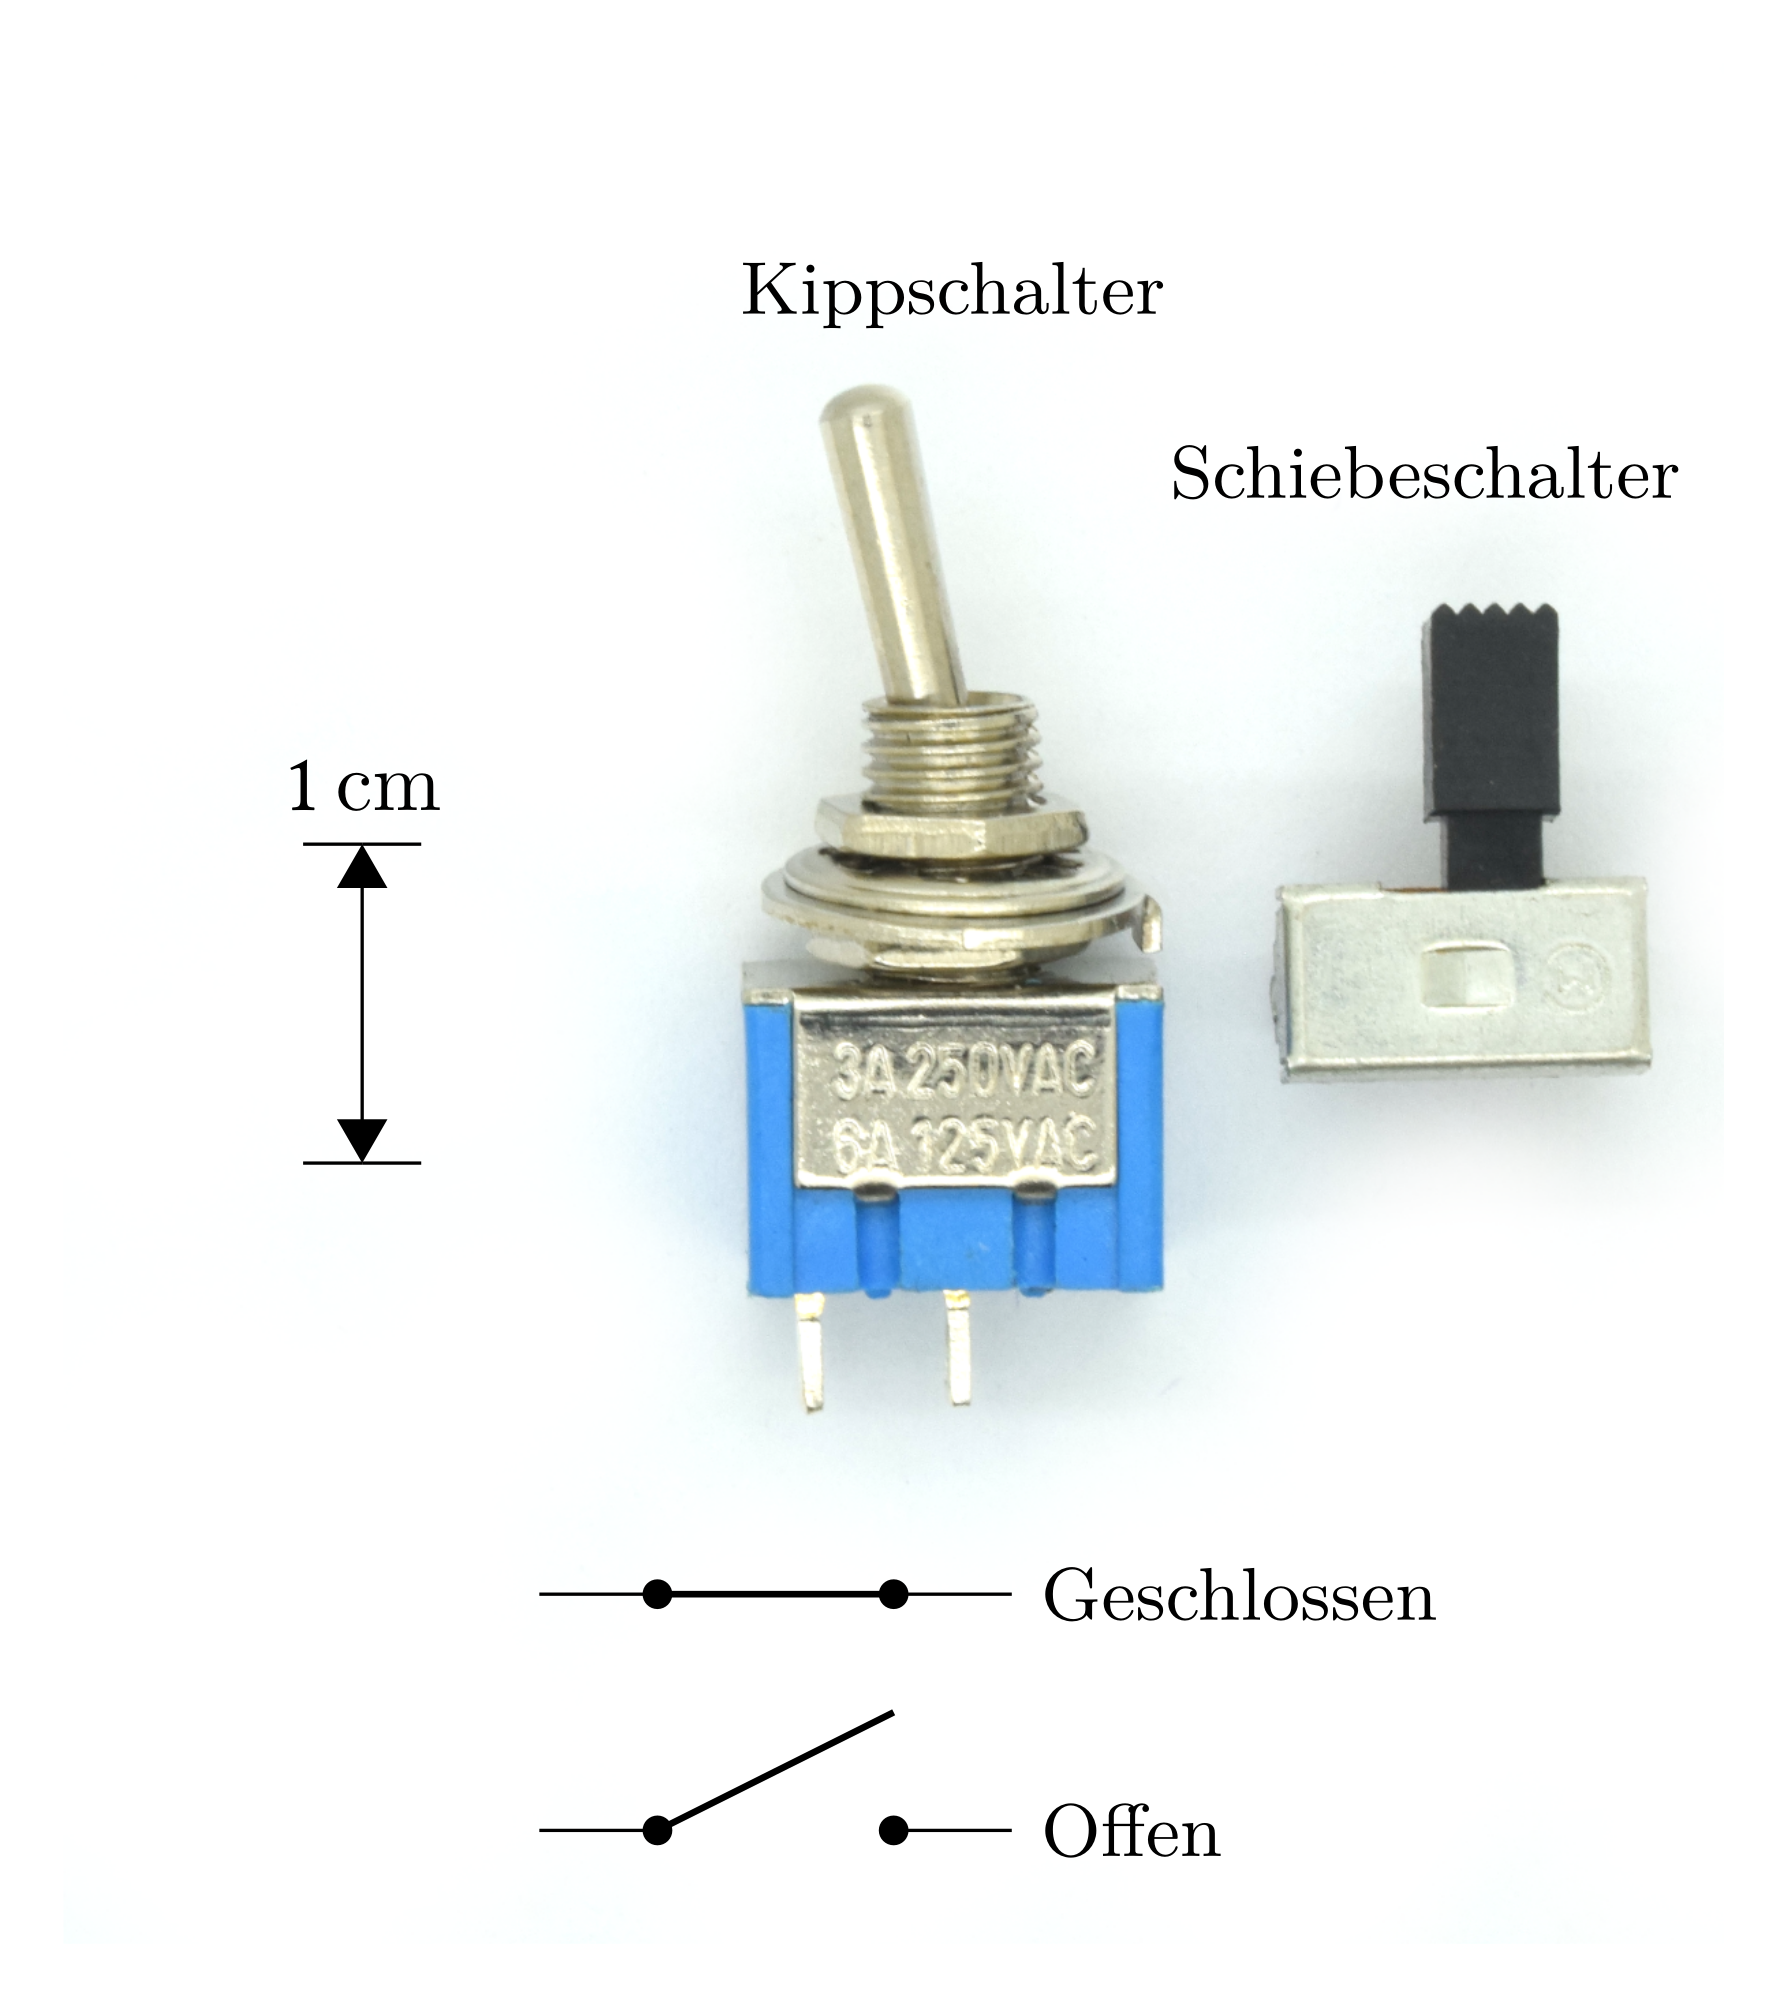
\includegraphics[width=0.85\textwidth]{foto/202}
    \caption{\scriptsize Schaltzeichen und Bauformen von Schaltern}
    \label{n_stromkreis_schalter}
\end{figure}

   \end{column}
\end{columns}

\end{frame}

\begin{frame}
\only<1>{
\begin{PQuestion}{NB701}{Welches Bauteil wird durch das Schaltzeichen symbolisiert?}{Masse}
{Schalter}
{Antenne}
{Erde}
{\DARCimage{0.5\linewidth}{546include}}\end{PQuestion}

}
\only<2>{
\begin{PQuestion}{NB701}{Welches Bauteil wird durch das Schaltzeichen symbolisiert?}{Masse}
{\textbf{\textcolor{DARCgreen}{Schalter}}}
{Antenne}
{Erde}
{\DARCimage{0.5\linewidth}{546include}}\end{PQuestion}

}
\end{frame}

\begin{frame}
\frametitle{Widerstand}
\begin{columns}
    \begin{column}{0.48\textwidth}
    \begin{itemize}
  \item Begrenzt den Stromfluss
  \item Wandelt Strom in Wärme um
  \end{itemize}

    \end{column}
   \begin{column}{0.48\textwidth}
       
\begin{figure}
    \includegraphics[width=0.85\textwidth]{foto/203}
    \caption{\scriptsize Schaltzeichen und Bauformen von Widerständen}
    \label{n_stromkreis_widerstand}
\end{figure}

   \end{column}
\end{columns}

\end{frame}

\begin{frame}
\only<1>{
\begin{PQuestion}{NC101}{Welches Bauteil wird durch das Schaltzeichen symbolisiert?}{Kondensator}
{Diode}
{Spule}
{Widerstand}
{\DARCimage{0.5\linewidth}{509include}}\end{PQuestion}

}
\only<2>{
\begin{PQuestion}{NC101}{Welches Bauteil wird durch das Schaltzeichen symbolisiert?}{Kondensator}
{Diode}
{Spule}
{\textbf{\textcolor{DARCgreen}{Widerstand}}}
{\DARCimage{0.5\linewidth}{509include}}\end{PQuestion}

}
\end{frame}

\begin{frame}
\frametitle{Stromrichtung}

\begin{figure}
    \DARCimage{0.85\linewidth}{662include}
    \caption{\scriptsize Geschlossener Stromkreis}
    \label{n_stromkreis_geschlossen}
\end{figure}

Vom Pluspol zum Minuspol: \emph{technische Stromrichtung}

\end{frame}

\begin{frame}
\only<1>{
\begin{question2x2}{NB702}{Welches Bild zeigt die technische Stromrichtung korrekt an?}{\DARCimage{1.0\linewidth}{536include}}
{\DARCimage{1.0\linewidth}{535include}}
{\DARCimage{1.0\linewidth}{537include}}
{\DARCimage{1.0\linewidth}{538include}}
\end{question2x2}

}
\only<2>{
\begin{question2x2}{NB702}{Welches Bild zeigt die technische Stromrichtung korrekt an?}{\DARCimage{1.0\linewidth}{536include}}
{\textbf{\textcolor{DARCgreen}{\DARCimage{1.0\linewidth}{535include}}}}
{\DARCimage{1.0\linewidth}{537include}}
{\DARCimage{1.0\linewidth}{538include}}
\end{question2x2}

}
\end{frame}

\begin{frame}
\only<1>{
\begin{PQuestion}{NB207}{Kann in folgender Schaltung von zwei gleichen Spannungsquellen Strom fließen? Welche Begründung ist richtig?}{Ja, weil der Pluspol mit dem Minuspol verbunden ist.}
{Nein, weil dies nur bei verschiedenen Spannungsquellen möglich ist.}
{Nein, weil kein geschlossener Stromkreis vorhanden ist.}
{Ja, weil die Spannungsquellen nie exakt identisch sind.}
{\DARCimage{1.0\linewidth}{451include}}\end{PQuestion}

}
\only<2>{
\begin{PQuestion}{NB207}{Kann in folgender Schaltung von zwei gleichen Spannungsquellen Strom fließen? Welche Begründung ist richtig?}{Ja, weil der Pluspol mit dem Minuspol verbunden ist.}
{Nein, weil dies nur bei verschiedenen Spannungsquellen möglich ist.}
{\textbf{\textcolor{DARCgreen}{Nein, weil kein geschlossener Stromkreis vorhanden ist.}}}
{Ja, weil die Spannungsquellen nie exakt identisch sind.}
{\DARCimage{1.0\linewidth}{451include}}\end{PQuestion}

}
\end{frame}%ENDCONTENT


\section{Spannungsmessung}
\label{section:spannungsmessung}
\begin{frame}%STARTCONTENT

\begin{columns}
    \begin{column}{0.48\textwidth}
    \begin{itemize}
  \item Spannungen lassen sich mit einem Messgerät ermitteln
  \item Schaltsymbol \enquote{V mit einem Kreis}
  \item Messgerät richtig einstellen
  \item An den richtigen Stellen messen
  \end{itemize}

    \end{column}
   \begin{column}{0.48\textwidth}
       
\begin{figure}
    \DARCimage{0.85\linewidth}{625include}
    \caption{\scriptsize Schaltsymbol Spannungsmessgerät}
    \label{n_messgeraete_symbol_spannungsmessgerät}
\end{figure}


   \end{column}
\end{columns}

\end{frame}

\begin{frame}
\frametitle{Richtig messen}
\begin{columns}
    \begin{column}{0.48\textwidth}
    \begin{itemize}
  \item Spannung wird zwischen zwei Punkten gemessen
  \item Parallel zum zu messenden Bauteil
  \end{itemize}

    \end{column}
   \begin{column}{0.48\textwidth}
       
\begin{figure}
    \DARCimage{0.85\linewidth}{620include}
    \caption{\scriptsize Spannungsmessung}
    \label{n_messgeraete_spannungsmessung}
\end{figure}


   \end{column}
\end{columns}

\end{frame}

\begin{frame}
\only<1>{
\begin{PQuestion}{NI101}{Was wird durch dieses Schaltzeichen symbolisiert?}{Stromquelle}
{Strommessgerät}
{Spannungsquelle}
{Spannungsmessgerät}
{\DARCimage{0.5\linewidth}{625include}}\end{PQuestion}

}
\only<2>{
\begin{PQuestion}{NI101}{Was wird durch dieses Schaltzeichen symbolisiert?}{Stromquelle}
{Strommessgerät}
{Spannungsquelle}
{\textbf{\textcolor{DARCgreen}{Spannungsmessgerät}}}
{\DARCimage{0.5\linewidth}{625include}}\end{PQuestion}

}
 \end{frame}

\begin{frame}
\only<1>{
\begin{question2x2}{NI103}{In welcher Schaltung ist ein Multimeter richtig eingesetzt, um die Spannung der Batterie im laufenden Betrieb zu messen?}{\DARCimage{0.75\linewidth}{623include}}
{\DARCimage{0.75\linewidth}{621include}}
{\DARCimage{0.75\linewidth}{622include}}
{\DARCimage{0.75\linewidth}{620include}}
\end{question2x2}

}
\only<2>{
\begin{question2x2}{NI103}{In welcher Schaltung ist ein Multimeter richtig eingesetzt, um die Spannung der Batterie im laufenden Betrieb zu messen?}{\DARCimage{0.75\linewidth}{623include}}
{\DARCimage{0.75\linewidth}{621include}}
{\DARCimage{0.75\linewidth}{622include}}
{\textbf{\textcolor{DARCgreen}{\DARCimage{0.75\linewidth}{620include}}}}
\end{question2x2}

}
\end{frame}

\begin{frame}
\only<1>{
\begin{PQuestion}{NB205}{Welchen Betrag zeigt das Spannungsmessgerät in folgender Schaltung? }{\qty{0}{\V}}
{\qty{3}{\V}}
{\qty{2,25}{\V}}
{\qty{1,5}{\V}}
{\DARCimage{1.0\linewidth}{626include}}\end{PQuestion}

}
\only<2>{
\begin{PQuestion}{NB205}{Welchen Betrag zeigt das Spannungsmessgerät in folgender Schaltung? }{\qty{0}{\V}}
{\textbf{\textcolor{DARCgreen}{\qty{3}{\V}}}}
{\qty{2,25}{\V}}
{\qty{1,5}{\V}}
{\DARCimage{1.0\linewidth}{626include}}\end{PQuestion}

}

\end{frame}

\begin{frame}
\only<1>{
\begin{PQuestion}{NB206}{Welche Spannung zeigt das Spannungsmessgerät in folgender Schaltung? }{\qty{1,5}{\V}}
{\qty{3}{\V}}
{\qty{-3}{\V}}
{\qty{0}{\V}}
{\DARCimage{1.0\linewidth}{452include}}\end{PQuestion}

}
\only<2>{
\begin{PQuestion}{NB206}{Welche Spannung zeigt das Spannungsmessgerät in folgender Schaltung? }{\qty{1,5}{\V}}
{\qty{3}{\V}}
{\qty{-3}{\V}}
{\textbf{\textcolor{DARCgreen}{\qty{0}{\V}}}}
{\DARCimage{1.0\linewidth}{452include}}\end{PQuestion}

}

\end{frame}%ENDCONTENT


\section{Strom messen}
\label{section:strommessung}
\begin{frame}%STARTCONTENT

\begin{columns}
    \begin{column}{0.48\textwidth}
    \begin{itemize}
  \item Strommessgeräte messen den elektischen Strom
  \item Schaltsymbol \enquote{A in einem Kreis} 
  \end{itemize}

    \end{column}
   \begin{column}{0.48\textwidth}
       
\begin{figure}
    \DARCimage{0.85\linewidth}{624include}
    \caption{\scriptsize Schaltsymbol Strommessgerät}
    \label{n_messgeraete_symbol_strommessgerät}
\end{figure}


   \end{column}
\end{columns}

\end{frame}

\begin{frame}
\frametitle{Richtig messen}
\begin{columns}
    \begin{column}{0.48\textwidth}
    \begin{itemize}
  \item Strom wird in Serie mit den Bauteilen gemessen
  \item Dadurch wird die Stromstärke durch das Bauteil ermittelt
  \end{itemize}

    \end{column}
   \begin{column}{0.48\textwidth}
       
\begin{figure}
    \DARCimage{0.85\linewidth}{616include}
    \caption{\scriptsize Strommessung}
    \label{n_messgeraete_strommessung}
\end{figure}


   \end{column}
\end{columns}

\end{frame}

\begin{frame}
\only<1>{
\begin{PQuestion}{NI102}{Was wird durch dieses Schaltzeichen symbolisiert?}{Spannungsquelle}
{Stromquelle}
{Spannungsmessgerät}
{Strommessgerät}
{\DARCimage{0.5\linewidth}{624include}}\end{PQuestion}

}
\only<2>{
\begin{PQuestion}{NI102}{Was wird durch dieses Schaltzeichen symbolisiert?}{Spannungsquelle}
{Stromquelle}
{Spannungsmessgerät}
{\textbf{\textcolor{DARCgreen}{Strommessgerät}}}
{\DARCimage{0.5\linewidth}{624include}}\end{PQuestion}

}
\end{frame}

\begin{frame}
\only<1>{
\begin{question2x2}{NI104}{In welcher Schaltung ist ein Multimeter richtig eingesetzt, um den Strom durch den Widerstand und die LED zu messen? }{\DARCimage{0.75\linewidth}{618include}}
{\DARCimage{0.75\linewidth}{617include}}
{\DARCimage{0.75\linewidth}{616include}}
{\DARCimage{0.75\linewidth}{619include}}
\end{question2x2}

}
\only<2>{
\begin{question2x2}{NI104}{In welcher Schaltung ist ein Multimeter richtig eingesetzt, um den Strom durch den Widerstand und die LED zu messen? }{\DARCimage{0.75\linewidth}{618include}}
{\DARCimage{0.75\linewidth}{617include}}
{\textbf{\textcolor{DARCgreen}{\DARCimage{0.75\linewidth}{616include}}}}
{\DARCimage{0.75\linewidth}{619include}}
\end{question2x2}

}
\end{frame}%ENDCONTENT


\section{Ohmsches Gesetz}
\label{section:ohmsches_gesetz}
\begin{frame}%STARTCONTENT
Kurze Wiederholung:

\begin{itemize}
  \item Elektrische Ladungen werden in Spannungesquellen getrennt, wodurch elektrische Spannung entsteht. Buchstabe $U$, Einheit Volt (V).
  \item Elektrische Spannung sorgt für elektrischen Stromfluss in geschlossenem Stromkreis. Buchstabe $I$, Einheit Ampere (A).
  \item Verbraucher üben in einem Stromkreis einen Widerstand aus und bremsen den Stromfluß. Buchstabe $R$, Einheit Ohm (Ω).
  \end{itemize}
\end{frame}

\begin{frame}
\only<1>{
\begin{QQuestion}{NA203}{Welche Einheit wird üblicherweise für den elektrische Widerstand verwendet?}{Volt (V)}
{Ohm ($\Omega$)}
{Ampere (A)}
{Watt (W)}
\end{QQuestion}

}
\only<2>{
\begin{QQuestion}{NA203}{Welche Einheit wird üblicherweise für den elektrische Widerstand verwendet?}{Volt (V)}
{\textbf{\textcolor{DARCgreen}{Ohm ($\Omega$)}}}
{Ampere (A)}
{Watt (W)}
\end{QQuestion}

}
\end{frame}

\begin{frame}
\frametitle{Zusammenhang}
\begin{columns}
    \begin{column}{0.48\textwidth}
    
\begin{figure}
    \DARCimage{0.85\linewidth}{664include}
    \caption{\scriptsize Stromkreis mit Batterie}
    \label{n_ohmsches_gesetz_stromkreis_mit_batterie}
\end{figure}


    \end{column}
   \begin{column}{0.48\textwidth}
       \begin{itemize}
  \item Spannung 10 V
  \item Strom 1 mA
  \end{itemize}

   \end{column}
\end{columns}

\end{frame}

\begin{frame}\begin{itemize}
  \item Bei 20 V erhöht sich der Strom auf 2 mA
  \item Bei 5 V verringert sich der Strom auf 0,5 mA
  \end{itemize}
    \pause
    $\dfrac{U}{I} = \dfrac{10 \ \text{V}}{0,001 \ \text{A}} = \dfrac{20 \ \text{V}}{0,002 \ \text{A}} = \dfrac{5 \ \text{V}}{0,0005 \ \text{A}} = 10000 \frac{\text{V}}{\text{A}}$
    \pause
    Proportionalität: $I$ ist proportional zu $U$ mit \emph{Proportionalitätsfaktor} 10000

\end{frame}

\begin{frame}
\frametitle{Widerstand}
\begin{itemize}
  \item Der Proportionalitätsfaktor von 10000 aus dem Beispiel ist der Widerstand $R$
  \item Einheit: $1 \ Ω = 1 \frac{\text{V}}{\text{A}}$
  \item Der Widerstand aus dem Beispiel beträgt 10000 Ω oder 10 kΩ
  \end{itemize}
\end{frame}

\begin{frame}
\frametitle{Ohmsches Gesetz}
Der Widerstand ist das \emph{Verhältnis von Spannung und Strom}

$ R = \dfrac{U}{I} $

\end{frame}

\begin{frame}
\only<1>{
\begin{PQuestion}{NB505}{Welcher Widerstandswert liegt vor?}{\qty{3,600}{\ohm}}
{\qty{40,000}{\ohm}}
{\qty{0,025}{\ohm}}
{\qty{0,200}{\ohm}}
{\DARCimage{0.75\linewidth}{508include}}\end{PQuestion}

}
\only<2>{
\begin{PQuestion}{NB505}{Welcher Widerstandswert liegt vor?}{\qty{3,600}{\ohm}}
{\textbf{\textcolor{DARCgreen}{\qty{40,000}{\ohm}}}}
{\qty{0,025}{\ohm}}
{\qty{0,200}{\ohm}}
{\DARCimage{0.75\linewidth}{508include}}\end{PQuestion}

}
\end{frame}

\begin{frame}
\frametitle{Formelumstellung}
\begin{columns}
    \begin{column}{0.48\textwidth}
    \begin{itemize}
  \item Spannung und Widerstand bekannt
  \item Strom unbekannt
  \end{itemize}
$ I = \dfrac{U}{R} $


    \end{column}
   \begin{column}{0.48\textwidth}
       \begin{itemize}
  \item Strom und Widerstand bekannt
  \item Spannung unbekannt
  \end{itemize}
$ U = R\cdot I $


   \end{column}
\end{columns}

\end{frame}

\begin{frame}
\only<1>{
\begin{PQuestion}{NB504}{Welche Spannung lässt einen Strom von \qty{90}{\mA} durch den Widerstand fließen?}{\qty{1,111}{\kV}}
{\qty{9,000}{\V}}
{\qty{9,000}{\kV}}
{\qty{1,111}{\V}}
{\DARCimage{0.75\linewidth}{507include}}\end{PQuestion}

}
\only<2>{
\begin{PQuestion}{NB504}{Welche Spannung lässt einen Strom von \qty{90}{\mA} durch den Widerstand fließen?}{\qty{1,111}{\kV}}
{\textbf{\textcolor{DARCgreen}{\qty{9,000}{\V}}}}
{\qty{9,000}{\kV}}
{\qty{1,111}{\V}}
{\DARCimage{0.75\linewidth}{507include}}\end{PQuestion}

}
\end{frame}

\begin{frame}
\only<1>{
\begin{QQuestion}{NB502}{Welcher der nachfolgenden Ausdrücke stellt den Zusammenhang zwischen Strom, Spannung und Widerstand korrekt dar?}{$R = U \cdot I$}
{$I = \dfrac{U}{R}$}
{$R = \dfrac{I}{U}$}
{$I =R \cdot U$}
\end{QQuestion}

}
\only<2>{
\begin{QQuestion}{NB502}{Welcher der nachfolgenden Ausdrücke stellt den Zusammenhang zwischen Strom, Spannung und Widerstand korrekt dar?}{$R = U \cdot I$}
{\textbf{\textcolor{DARCgreen}{$I = \dfrac{U}{R}$}}}
{$R = \dfrac{I}{U}$}
{$I =R \cdot U$}
\end{QQuestion}

}
\end{frame}

\begin{frame}
\only<1>{
\begin{QQuestion}{NB503}{Welcher der nachfolgenden Ausdrücke stellt den Zusammenhang zwischen Strom, Spannung und Widerstand korrekt dar?}{$R = \dfrac{U}{I}$}
{$R = U \cdot I$}
{$R = \dfrac{I}{U}$}
{$I =R \cdot U$}
\end{QQuestion}

}
\only<2>{
\begin{QQuestion}{NB503}{Welcher der nachfolgenden Ausdrücke stellt den Zusammenhang zwischen Strom, Spannung und Widerstand korrekt dar?}{\textbf{\textcolor{DARCgreen}{$R = \dfrac{U}{I}$}}}
{$R = U \cdot I$}
{$R = \dfrac{I}{U}$}
{$I =R \cdot U$}
\end{QQuestion}

}
\end{frame}

\begin{frame}
\only<1>{
\begin{QQuestion}{NB501}{Welcher der nachfolgenden Ausdrücke stellt den Zusammenhang zwischen Strom, Spannung und Widerstand korrekt dar?}{$R = U \cdot I$}
{$U = R \cdot I $}
{$R = \dfrac{I}{U}$}
{$I =R \cdot U$}
\end{QQuestion}

}
\only<2>{
\begin{QQuestion}{NB501}{Welcher der nachfolgenden Ausdrücke stellt den Zusammenhang zwischen Strom, Spannung und Widerstand korrekt dar?}{$R = U \cdot I$}
{\textbf{\textcolor{DARCgreen}{$U = R \cdot I $}}}
{$R = \dfrac{I}{U}$}
{$I =R \cdot U$}
\end{QQuestion}

}
\end{frame}%ENDCONTENT


\section{Widerstandsfarbcode}
\label{section:widerstandsfarbcode}
\begin{frame}%STARTCONTENT

\begin{columns}
    \begin{column}{0.48\textwidth}
    
\begin{figure}
    \DARCimage{0.85\linewidth}{665include}
    \caption{\scriptsize  Ein Widerstand mit 4 Farbringen}
    \label{n_widerstandsfarbcodes}
\end{figure}


    \end{column}
   \begin{column}{0.48\textwidth}
       \begin{table}
\begin{DARCtabular}{Xlll}
    Farbe  &Wert  &Multiplikator  &Toleranz   \\
     Silber  & --  & 0,01  &  $\pm$ \qty{10}{\percent}   \\
     Gold  & --  & 0,1 &  $\pm$ \qty{5}{\percent}   \\
     Schwarz  & 0  & 1  & --   \\
     Braun  & 1  & 10  &  $\pm$ \qty{1}{\percent}   \\
     Rot  & 2  & 100  &  $\pm$ \qty{2}{\percent}   \\
     Orange & 3  & 1000  & --   \\
     Gelb  & 4  & 10000  & --   \\
     Grün  & 5  & 100000  & --   \\
     Blau  & 6  & 1000000  &  $\pm$ \qty{0,25}{\percent}  \\
     Violett  & 7  & 10000000  &  $\pm$ \qty{0,1}{\percent}  \\
     Grau  & 8  & 100000000  & --   \\
     Weiß  & 9  & 1000000000  & --   \\
     Keine  & --  & --  &  $\pm$ \qty{20}{\percent}  \\
\end{DARCtabular}
\caption{Widerstandsfarbcodes Tabelle}
\label{n_widerstandsfarbcodes_tabelle}
\end{table}

   \end{column}
\end{columns}

\end{frame}

\begin{frame}
\frametitle{Toleranz}
\begin{itemize}
  \item Abweichung vom tatsächlichen Wert
  \item Beispiel: silber bedeutet  $\pm$ \qty{10}{\percent}
  \item \qty{10}{\percent} von 47 kΩ = 4,7 kΩ
  \item Widerstandswert zwischen 42,3 kΩ und 51,7 kΩ
  \end{itemize}
\end{frame}

\begin{frame}
\only<1>{
\begin{QQuestion}{NC107}{Die Farbringe gelb, violett und orange auf einem Widerstand mit 4 Farbringen bedeuten einen Widerstandswert von~...}{\qty{4,7}{\kohm}.}
{\qty{47}{\kohm}.}
{\qty{470}{\kohm}.}
{\qty{4,7}{\Mohm}.}
\end{QQuestion}

}
\only<2>{
\begin{QQuestion}{NC107}{Die Farbringe gelb, violett und orange auf einem Widerstand mit 4 Farbringen bedeuten einen Widerstandswert von~...}{\qty{4,7}{\kohm}.}
{\textbf{\textcolor{DARCgreen}{\qty{47}{\kohm}.}}}
{\qty{470}{\kohm}.}
{\qty{4,7}{\Mohm}.}
\end{QQuestion}

}
\end{frame}

\begin{frame}
\only<1>{
\begin{QQuestion}{NC105}{Die Farbringe gelb, violett und rot auf einem Widerstand mit 4 Farbringen bedeuten einen Widerstandswert von~...}{\qty{4,7}{\Mohm}.}
{\qty{47}{\kohm}.}
{\qty{470}{\kohm}.}
{\qty{4,7}{\kohm}.}
\end{QQuestion}

}
\only<2>{
\begin{QQuestion}{NC105}{Die Farbringe gelb, violett und rot auf einem Widerstand mit 4 Farbringen bedeuten einen Widerstandswert von~...}{\qty{4,7}{\Mohm}.}
{\qty{47}{\kohm}.}
{\qty{470}{\kohm}.}
{\textbf{\textcolor{DARCgreen}{\qty{4,7}{\kohm}.}}}
\end{QQuestion}

}
\end{frame}

\begin{frame}
\only<1>{
\begin{QQuestion}{NC106}{Die Farbringe rot, violett und orange auf einem Widerstand mit 4 Farbringen bedeuten einen Widerstandswert von~...}{\qty{2,7}{\kohm}.}
{\qty{27}{\kohm}.}
{\qty{270}{\kohm}.}
{\qty{2,7}{\Mohm}.}
\end{QQuestion}

}
\only<2>{
\begin{QQuestion}{NC106}{Die Farbringe rot, violett und orange auf einem Widerstand mit 4 Farbringen bedeuten einen Widerstandswert von~...}{\qty{2,7}{\kohm}.}
{\textbf{\textcolor{DARCgreen}{\qty{27}{\kohm}.}}}
{\qty{270}{\kohm}.}
{\qty{2,7}{\Mohm}.}
\end{QQuestion}

}
\end{frame}

\begin{frame}
\only<1>{
\begin{QQuestion}{NC104}{Die Farbringe rot, violett und rot auf einem Widerstand mit 4 Farbringen bedeuten einen Widerstandswert von~...}{\qty{27}{\kohm}.}
{\qty{2,7}{\kohm}.}
{\qty{270}{\kohm}.}
{\qty{2,7}{\Mohm}.}
\end{QQuestion}

}
\only<2>{
\begin{QQuestion}{NC104}{Die Farbringe rot, violett und rot auf einem Widerstand mit 4 Farbringen bedeuten einen Widerstandswert von~...}{\qty{27}{\kohm}.}
{\textbf{\textcolor{DARCgreen}{\qty{2,7}{\kohm}.}}}
{\qty{270}{\kohm}.}
{\qty{2,7}{\Mohm}.}
\end{QQuestion}

}
\end{frame}

\begin{frame}
\only<1>{
\begin{QQuestion}{NC103}{Welche drei Farbringe hat ein \qty{1,2}{\kohm} Widerstand am Anfang, wenn vier Farbringe verwendet werden?}{Braun, rot, rot}
{Rot, orange, braun}
{Braun, rot, orange}
{Rot, braun, rot}
\end{QQuestion}

}
\only<2>{
\begin{QQuestion}{NC103}{Welche drei Farbringe hat ein \qty{1,2}{\kohm} Widerstand am Anfang, wenn vier Farbringe verwendet werden?}{\textbf{\textcolor{DARCgreen}{Braun, rot, rot}}}
{Rot, orange, braun}
{Braun, rot, orange}
{Rot, braun, rot}
\end{QQuestion}

}
\end{frame}

\begin{frame}
\only<1>{
\begin{QQuestion}{NC102}{Welchem Multiplikator entspricht ein grüner Farbring auf einem Widerstand mit 4 Farbringen?}{\num{10000}}
{\num{100000}}
{\num{1000000}}
{\num{10000000}}
\end{QQuestion}

}
\only<2>{
\begin{QQuestion}{NC102}{Welchem Multiplikator entspricht ein grüner Farbring auf einem Widerstand mit 4 Farbringen?}{\num{10000}}
{\textbf{\textcolor{DARCgreen}{\num{100000}}}}
{\num{1000000}}
{\num{10000000}}
\end{QQuestion}

}
\end{frame}

\begin{frame}
\only<1>{
\begin{QQuestion}{NC108}{Welche Toleranz weist ein Widerstand mit 4 Farbcodes auf, wenn der vierte Farbring ein silberner Farbring ist?}{ $\pm$\qty{5}{\percent}}
{ $\pm$\qty{10}{\percent}}
{ $\pm$\qty{0,1}{\percent}}
{ $\pm$\qty{1}{\percent}}
\end{QQuestion}

}
\only<2>{
\begin{QQuestion}{NC108}{Welche Toleranz weist ein Widerstand mit 4 Farbcodes auf, wenn der vierte Farbring ein silberner Farbring ist?}{ $\pm$\qty{5}{\percent}}
{\textbf{\textcolor{DARCgreen}{ $\pm$\qty{10}{\percent}}}}
{ $\pm$\qty{0,1}{\percent}}
{ $\pm$\qty{1}{\percent}}
\end{QQuestion}

}
\end{frame}

\begin{frame}
\only<1>{
\begin{QQuestion}{NC109}{Welche Toleranz weist ein Widerstand mit 4 Farbcodes auf, wenn der vierte Farbring ein goldener Farbring ist?}{ $\pm$\qty{0,5}{\percent}}
{ $\pm$\qty{5}{\percent}}
{ $\pm$\qty{0,1}{\percent}}
{ $\pm$\qty{1}{\percent}}
\end{QQuestion}

}
\only<2>{
\begin{QQuestion}{NC109}{Welche Toleranz weist ein Widerstand mit 4 Farbcodes auf, wenn der vierte Farbring ein goldener Farbring ist?}{ $\pm$\qty{0,5}{\percent}}
{\textbf{\textcolor{DARCgreen}{ $\pm$\qty{5}{\percent}}}}
{ $\pm$\qty{0,1}{\percent}}
{ $\pm$\qty{1}{\percent}}
\end{QQuestion}

}
\end{frame}

\begin{frame}
\only<1>{
\begin{QQuestion}{NC110}{Welche Toleranz weist ein Widerstand mit 4 Farbcodes auf, wenn der vierte Farbring braun ist?}{$\pm$\qty{5}{\percent}}
{$\pm$\qty{0,1}{\percent}}
{$\pm$\qty{1}{\percent}}
{$\pm$\qty{10}{\percent}}
\end{QQuestion}

}
\only<2>{
\begin{QQuestion}{NC110}{Welche Toleranz weist ein Widerstand mit 4 Farbcodes auf, wenn der vierte Farbring braun ist?}{$\pm$\qty{5}{\percent}}
{$\pm$\qty{0,1}{\percent}}
{\textbf{\textcolor{DARCgreen}{$\pm$\qty{1}{\percent}}}}
{$\pm$\qty{10}{\percent}}
\end{QQuestion}

}
\end{frame}%ENDCONTENT


\section{Halbleiter}
\label{section:halbleiter}
\begin{frame}%STARTCONTENT
\begin{itemize}
  \item Weisen Eigenschaften von Leitern als auch von Nichtleitern auf
  \item Häufige Halbleiterelemente: Silizium oder Germanium
  \end{itemize}

\end{frame}

\begin{frame}
\frametitle{Diode}
\begin{columns}
    \begin{column}{0.48\textwidth}
    \begin{itemize}
  \item Einfachstes Halbleiter-Bauteil: Diode
  \item Strom kann nur in einer Richtung durch sie hindurchfließen
  \end{itemize}

    \end{column}
   \begin{column}{0.48\textwidth}
       
\begin{figure}
    \includegraphics[width=0.85\textwidth]{foto/204}
    \caption{\scriptsize Schaltzeichen und Bauformen von Dioden}
    \label{n_halbleiter_dioden}
\end{figure}

   \end{column}
\end{columns}

\end{frame}

\begin{frame}
\only<1>{
\begin{PQuestion}{NC401}{Welches Bauteil wird durch das Schaltzeichen symbolisiert?}{Spule}
{Widerstand}
{Diode}
{Kondensator}
{\DARCimage{0.5\linewidth}{381include}}\end{PQuestion}

}
\only<2>{
\begin{PQuestion}{NC401}{Welches Bauteil wird durch das Schaltzeichen symbolisiert?}{Spule}
{Widerstand}
{\textbf{\textcolor{DARCgreen}{Diode}}}
{Kondensator}
{\DARCimage{0.5\linewidth}{381include}}\end{PQuestion}

}
\end{frame}

\begin{frame}
\frametitle{Anschlüsse einer Diode}
\begin{columns}
    \begin{column}{0.48\textwidth}
    \begin{itemize}
  \item Anode und Kathode
  \item Plus-Pol an Anode und Minus-Pol an Kathode: \emph{Diode leitet}
  \item Plus-Pol an Kathode und Minus-Pol an Anode: \emph{Diode sperrt}
  \end{itemize}

    \end{column}
   \begin{column}{0.48\textwidth}
       
\begin{figure}
    \DARCimage{0.85\linewidth}{666include}
    \caption{\scriptsize Merkhilfe Diode}
    \label{n_halbleiter_diode_merkhilfe}
\end{figure}


   \end{column}
\end{columns}

\end{frame}

\begin{frame}
\only<1>{
\begin{PQuestion}{NC403}{Wie lauten die Bezeichnungen für die Anschlüsse 1 und 2 im Schaltsymbol?}{1 = Anode; 2 = Kathode}
{1 = Kathode; 2 = Anode}
{1 = Basis; 2 = Kathode}
{1 = Emitter; 2 = Anode}
{\DARCimage{0.5\linewidth}{383include}}\end{PQuestion}

}
\only<2>{
\begin{PQuestion}{NC403}{Wie lauten die Bezeichnungen für die Anschlüsse 1 und 2 im Schaltsymbol?}{\textbf{\textcolor{DARCgreen}{1 = Anode; 2 = Kathode}}}
{1 = Kathode; 2 = Anode}
{1 = Basis; 2 = Kathode}
{1 = Emitter; 2 = Anode}
{\DARCimage{0.5\linewidth}{383include}}\end{PQuestion}

}
\end{frame}

\begin{frame}
\only<1>{
\begin{question2x2}{NC404}{In welchem der abgebildeten Stromkreise fließt Strom?}{\DARCimage{0.75\linewidth}{520include}}
{\DARCimage{0.75\linewidth}{519include}}
{\DARCimage{0.75\linewidth}{518include}}
{\DARCimage{0.75\linewidth}{521include}}
\end{question2x2}

}
\only<2>{
\begin{question2x2}{NC404}{In welchem der abgebildeten Stromkreise fließt Strom?}{\DARCimage{0.75\linewidth}{520include}}
{\DARCimage{0.75\linewidth}{519include}}
{\textbf{\textcolor{DARCgreen}{\DARCimage{0.75\linewidth}{518include}}}}
{\DARCimage{0.75\linewidth}{521include}}
\end{question2x2}

}
\end{frame}

\begin{frame}
\frametitle{LED}
\begin{columns}
    \begin{column}{0.48\textwidth}
    \begin{itemize}
  \item Leuchtdiode, \enquote{light-emitting diode}
  \item Leuchtet, sobald Strom durch sie hindurchfließt
  \item Schaltbild: Diode mit zwei zusätzlichen Pfeilen nach außen
  \item Verhält sich wie Diode, aber leuchtet
  \end{itemize}

    \end{column}
   \begin{column}{0.48\textwidth}
       
\begin{figure}
    \includegraphics[width=0.85\textwidth]{foto/205}
    \caption{\scriptsize Schaltzeichen und Bauformen von LEDs}
    \label{n_halbleiter_led}
\end{figure}

   \end{column}
\end{columns}

\end{frame}

\begin{frame}
\only<1>{
\begin{PQuestion}{NC402}{Welches Bauteil wird durch das Schaltzeichen symbolisiert?}{Batterie}
{Spule}
{Kondensator}
{Leuchtdiode}
{\DARCimage{0.5\linewidth}{522include}}\end{PQuestion}

}
\only<2>{
\begin{PQuestion}{NC402}{Welches Bauteil wird durch das Schaltzeichen symbolisiert?}{Batterie}
{Spule}
{Kondensator}
{\textbf{\textcolor{DARCgreen}{Leuchtdiode}}}
{\DARCimage{0.5\linewidth}{522include}}\end{PQuestion}

}
\end{frame}

\begin{frame}
\only<1>{
\begin{question2x2}{NB703}{Bei welchem der abgebildeten Stromkreise leuchtet die LED?}{\DARCimage{0.75\linewidth}{513include}}
{\DARCimage{0.75\linewidth}{514include}}
{\DARCimage{0.75\linewidth}{515include}}
{\DARCimage{0.75\linewidth}{516include}}
\end{question2x2}

}
\only<2>{
\begin{question2x2}{NB703}{Bei welchem der abgebildeten Stromkreise leuchtet die LED?}{\textbf{\textcolor{DARCgreen}{\DARCimage{0.75\linewidth}{513include}}}}
{\DARCimage{0.75\linewidth}{514include}}
{\DARCimage{0.75\linewidth}{515include}}
{\DARCimage{0.75\linewidth}{516include}}
\end{question2x2}

}
\end{frame}%ENDCONTENT


\section{Leistung}
\label{section:leistung}
\begin{frame}%STARTCONTENT
\begin{itemize}
  \item Elektrische Geräte haben eine Leistungsaufnahme angegeben
  \item Beispiele: LED-Leuchtmittel 7 W, Staubsauger 425 W
  \item An jedem Widerstand wird elektrische Leistung umgesetzt
  \item Strom fließt durch einen Widerstand $\rightarrow$ Umwandlung von elektrischer Energie in thermische Energie
  \item Je größer der Strom, desto mehr Wärme
  \end{itemize}
\end{frame}

\begin{frame}
\only<1>{
\begin{QQuestion}{NA204}{Welche Einheit wird üblicherweise für die elektrische Leistung verwendet?}{Kilowattstunden (kWh)}
{Watt (W)}
{Joule (J)}
{Amperestunden (Ah)}
\end{QQuestion}

}
\only<2>{
\begin{QQuestion}{NA204}{Welche Einheit wird üblicherweise für die elektrische Leistung verwendet?}{Kilowattstunden (kWh)}
{\textbf{\textcolor{DARCgreen}{Watt (W)}}}
{Joule (J)}
{Amperestunden (Ah)}
\end{QQuestion}

}
\end{frame}

\begin{frame}
\only<1>{
\begin{QQuestion}{NA211}{\qty{0,010}{\W} entspricht ...}{\qty{10}{\mW}}
{\qty{10}{\micro\W}}
{\qty{100}{\nano\W}}
{\qty{100}{\pico\W}}
\end{QQuestion}

}
\only<2>{
\begin{QQuestion}{NA211}{\qty{0,010}{\W} entspricht ...}{\textbf{\textcolor{DARCgreen}{\qty{10}{\mW}}}}
{\qty{10}{\micro\W}}
{\qty{100}{\nano\W}}
{\qty{100}{\pico\W}}
\end{QQuestion}

}
\end{frame}

\begin{frame}
\only<1>{
\begin{QQuestion}{NA210}{\qty{1}{\W} entspricht ...}{\qty{1000}{\micro\W}}
{\qty{1000}{\mW}}
{\qty{1000}{\nano\W}}
{\qty{1000}{\pico\W}}
\end{QQuestion}

}
\only<2>{
\begin{QQuestion}{NA210}{\qty{1}{\W} entspricht ...}{\qty{1000}{\micro\W}}
{\textbf{\textcolor{DARCgreen}{\qty{1000}{\mW}}}}
{\qty{1000}{\nano\W}}
{\qty{1000}{\pico\W}}
\end{QQuestion}

}
\end{frame}

\begin{frame}
\frametitle{Berechnung der Leistung}
Abhängig von Strom und Spannung

$ P = U \cdot I $

$ U = \dfrac{P}{I} $

$ I = \dfrac{P}{U} $

\end{frame}

\begin{frame}
\only<1>{
\begin{QQuestion}{NB601}{Welche Leistung nimmt ein Transceiver bei \qty{13,8}{\V} Gleichspannung auf, wenn das Strommessgerät im Netzteil \qty{1,5}{\A} anzeigt?}{\qty{9,2}{\W}}
{\qty{1,53}{\W}}
{\qty{2,07}{\W}}
{\qty{20,7}{\W}}
\end{QQuestion}

}
\only<2>{
\begin{QQuestion}{NB601}{Welche Leistung nimmt ein Transceiver bei \qty{13,8}{\V} Gleichspannung auf, wenn das Strommessgerät im Netzteil \qty{1,5}{\A} anzeigt?}{\qty{9,2}{\W}}
{\qty{1,53}{\W}}
{\qty{2,07}{\W}}
{\textbf{\textcolor{DARCgreen}{\qty{20,7}{\W}}}}
\end{QQuestion}

}
\end{frame}

\begin{frame}
\only<1>{
\begin{QQuestion}{NB602}{An einem Vorwiderstand fällt bei einem Strom von \qty{50}{\mA} eine Spannung von \qty{50}{\V} ab. Wieviel Leistung wird an diesem in Wärme umgesetzt?}{\qty{2,5}{\W}}
{\qty{1}{\kW}}
{\qty{1}{\W}}
{\qty{250}{\mW}}
\end{QQuestion}

}
\only<2>{
\begin{QQuestion}{NB602}{An einem Vorwiderstand fällt bei einem Strom von \qty{50}{\mA} eine Spannung von \qty{50}{\V} ab. Wieviel Leistung wird an diesem in Wärme umgesetzt?}{\textbf{\textcolor{DARCgreen}{\qty{2,5}{\W}}}}
{\qty{1}{\kW}}
{\qty{1}{\W}}
{\qty{250}{\mW}}
\end{QQuestion}

}
\end{frame}

\begin{frame}
\only<1>{
\begin{QQuestion}{NB603}{An einem Vorwiderstand fällt bei einem Strom von \qty{20}{\mA} eine Spannung von \qty{3,2}{\V} ab. Wieviel Leistung wird an diesem in Wärme umgesetzt?}{\qty{64,0}{\mW}}
{\qty{0,16}{\mW}}
{\qty{6,25}{\mW}}
{\qty{20}{\mW}}
\end{QQuestion}

}
\only<2>{
\begin{QQuestion}{NB603}{An einem Vorwiderstand fällt bei einem Strom von \qty{20}{\mA} eine Spannung von \qty{3,2}{\V} ab. Wieviel Leistung wird an diesem in Wärme umgesetzt?}{\textbf{\textcolor{DARCgreen}{\qty{64,0}{\mW}}}}
{\qty{0,16}{\mW}}
{\qty{6,25}{\mW}}
{\qty{20}{\mW}}
\end{QQuestion}

}
\end{frame}

\begin{frame}
\only<1>{
\begin{QQuestion}{NB606}{Ein gleichspannungsbetriebenes Leuchtmittel ist mit der Angabe \qty{12}{\V} / \qty{48}{\W} bedruckt.  Bei einer \qty{12}{\V}-Versorgung beträgt die Stromentnahme~...}{\qty{4}{\A}.}
{\qty{250}{\mA}.}
{\qty{750}{\mA}.}
{\qty{36}{\A}.}
\end{QQuestion}

}
\only<2>{
\begin{QQuestion}{NB606}{Ein gleichspannungsbetriebenes Leuchtmittel ist mit der Angabe \qty{12}{\V} / \qty{48}{\W} bedruckt.  Bei einer \qty{12}{\V}-Versorgung beträgt die Stromentnahme~...}{\textbf{\textcolor{DARCgreen}{\qty{4}{\A}.}}}
{\qty{250}{\mA}.}
{\qty{750}{\mA}.}
{\qty{36}{\A}.}
\end{QQuestion}

}
\end{frame}

\begin{frame}
\only<1>{
\begin{QQuestion}{NB604}{Ein Mobil-Transceiver (Sendeempfänger) wird aus dem Bordnetz eines Kraftfahrzeuges mit \qty{12}{\V}~Nennspannung betrieben und hat bei Sendebetrieb eine Leistungsaufnahme von \qty{100}{\W}. Wie groß ist dann die Stromaufnahme?}{\qty{0,12}{\A}}
{\qty{16,6}{\A}}
{\qty{1200}{\A}}
{\qty{8,33}{\A}}
\end{QQuestion}

}
\only<2>{
\begin{QQuestion}{NB604}{Ein Mobil-Transceiver (Sendeempfänger) wird aus dem Bordnetz eines Kraftfahrzeuges mit \qty{12}{\V}~Nennspannung betrieben und hat bei Sendebetrieb eine Leistungsaufnahme von \qty{100}{\W}. Wie groß ist dann die Stromaufnahme?}{\qty{0,12}{\A}}
{\qty{16,6}{\A}}
{\qty{1200}{\A}}
{\textbf{\textcolor{DARCgreen}{\qty{8,33}{\A}}}}
\end{QQuestion}

}
 \end{frame}

\begin{frame}
\only<1>{
\begin{QQuestion}{NB605}{Ein Leuchtmittel hat einen Nennwert von \qty{12}{\V} und \qty{3}{\W}. Wie viel Strom fließt beim Anschluss an \qty{12}{\V}?}{\qty{2,5}{\A}}
{\qty{400}{\mA}}
{\qty{4}{\A}}
{\qty{250}{\mA}}
\end{QQuestion}

}
\only<2>{
\begin{QQuestion}{NB605}{Ein Leuchtmittel hat einen Nennwert von \qty{12}{\V} und \qty{3}{\W}. Wie viel Strom fließt beim Anschluss an \qty{12}{\V}?}{\qty{2,5}{\A}}
{\qty{400}{\mA}}
{\qty{4}{\A}}
{\textbf{\textcolor{DARCgreen}{\qty{250}{\mA}}}}
\end{QQuestion}

}
\end{frame}%ENDCONTENT


\section{Schaltzeichen und Bauelemente}
\label{section:bauelemente}
\begin{frame}%STARTCONTENT
\begin{itemize}
  \item Drei weitere grundlegende Bauteile
  \item Funktionsweise ist Stoff für Klasse~E und A
  \item Für die Prüfung: Schaltzeichen erkennen
  \end{itemize}
\end{frame}

\begin{frame}
\frametitle{Kondensator}
\begin{columns}
    \begin{column}{0.48\textwidth}
    \begin{itemize}
  \item Speichert eine kleine Menge Energie
  \item Besteht oft aus zwei parallelen Platten
  \end{itemize}

    \end{column}
   \begin{column}{0.48\textwidth}
       
\begin{figure}
    \includegraphics[width=0.85\textwidth]{foto/206}
    \caption{\scriptsize Schaltzeichen und Bauformen von Kondensatoren}
    \label{n_bauelemente_kondensator}
\end{figure}

   \end{column}
\end{columns}

\end{frame}

\begin{frame}
\only<1>{
\begin{PQuestion}{NC201}{Welches Bauteil wird durch das Schaltzeichen symbolisiert?}{Transistor}
{Spule}
{Kondensator}
{Batterie}
{\DARCimage{0.5\linewidth}{511include}}\end{PQuestion}

}
\only<2>{
\begin{PQuestion}{NC201}{Welches Bauteil wird durch das Schaltzeichen symbolisiert?}{Transistor}
{Spule}
{\textbf{\textcolor{DARCgreen}{Kondensator}}}
{Batterie}
{\DARCimage{0.5\linewidth}{511include}}\end{PQuestion}

}
\end{frame}

\begin{frame}
\frametitle{Spule}
\begin{columns}
    \begin{column}{0.48\textwidth}
    \begin{itemize}
  \item Speichert auch eine kleine Menge Energie
  \item Funktioniert technisch aber komplett anders als der Kondensator
  \item Besteht in den einfachen Fällen aus einem aufgewickelten Draht
  \end{itemize}

    \end{column}
   \begin{column}{0.48\textwidth}
       
\begin{figure}
    \includegraphics[width=0.85\textwidth]{foto/207}
    \caption{\scriptsize Schaltzeichen und Bauformen von Spulen}
    \label{n_bauelemente_spule}
\end{figure}

   \end{column}
\end{columns}

\end{frame}

\begin{frame}
\only<1>{
\begin{PQuestion}{NC301}{Welches Bauteil wird durch das Schaltzeichen symbolisiert?}{Diode}
{Kondensator}
{Spule}
{Batterie}
{\DARCimage{0.5\linewidth}{512include}}\end{PQuestion}

}
\only<2>{
\begin{PQuestion}{NC301}{Welches Bauteil wird durch das Schaltzeichen symbolisiert?}{Diode}
{Kondensator}
{\textbf{\textcolor{DARCgreen}{Spule}}}
{Batterie}
{\DARCimage{0.5\linewidth}{512include}}\end{PQuestion}

}
\end{frame}

\begin{frame}
\frametitle{Transistor}
\begin{columns}
    \begin{column}{0.48\textwidth}
    \begin{itemize}
  \item Elektrischer Schalter
  \item Oder Verstärker, je nach Beschaltung
  \item Hat drei Anschlüsse
  \end{itemize}

    \end{column}
   \begin{column}{0.48\textwidth}
       
\begin{figure}
    \includegraphics[width=0.85\textwidth]{foto/208}
    \caption{\scriptsize Schaltzeichen und Bauformen von Transistoren}
    \label{n_bauelemente_transistor}
\end{figure}

   \end{column}
\end{columns}

\end{frame}

\begin{frame}
\only<1>{
\begin{PQuestion}{NC501}{Welches Bauteil wird durch das Schaltzeichen symbolisiert?}{Diode}
{Spule}
{Kondensator}
{Transistor}
{\DARCimage{0.25\linewidth}{374include}}\end{PQuestion}

}
\only<2>{
\begin{PQuestion}{NC501}{Welches Bauteil wird durch das Schaltzeichen symbolisiert?}{Diode}
{Spule}
{Kondensator}
{\textbf{\textcolor{DARCgreen}{Transistor}}}
{\DARCimage{0.25\linewidth}{374include}}\end{PQuestion}

}
\end{frame}%ENDCONTENT


\title{DARC Amateurfunklehrgang Klasse N}
\author{Gesetze und Vorschriften}
\institute{Deutscher Amateur Radio Club e.\,V.}
\begin{frame}
\maketitle
\end{frame}

\section{Internationale Vereinbarungen, Gesetze und Vorschriften}
\label{section:gesetze_vorschriften}
\begin{frame}%STARTCONTENT

\frametitle{Internationale Vereinbarungen}
\begin{itemize}
  \item Die allgemeinen Regelungen der ITU Radio Regulations (RR) gelten auch für den Amateurfunkdienst.
  \item Hinzu kommen Empfehlungen der Europäischen Konferenz der Verwaltungen für Post und Telekommunikation (CEPT).
  \end{itemize}
\end{frame}

\begin{frame}
\frametitle{Gesetze und Vorschriften}
Die internationalen Vereinbarungen gelten nicht direkt für Funkamateure, sondern ihre Umsetzung in die nationalen Gesetze und Verordnungen eines Landes.

\end{frame}

\begin{frame}Deswegen ist in Deutschland maßgeblich:

\begin{itemize}
  \item Das Gesetz über den Amateurfunk (AFuG) bildet die Rechtsgrundlage für die Teilnahme am Amateurfunkdienst in Deutschland.
  \item Details regelt die Amateurfunkverordnung (AFuV).
  \item Die Aufgaben und Befugnisse, die aus dem AFuG und der AFuV erwachsen, nimmt die Bundesnetzagentur (BNetzA) wahr.
  \item Auch das Telekommunikationsgesetz (TKG) enthält Regelungen, die auf den Amateurfunkdienst anwendbar sind.
  \end{itemize}

\end{frame}

\begin{frame}
\only<1>{
\begin{QQuestion}{VA301}{Die allgemeinen Regelungen der Radio Regulations (RR) gelten~...}{lediglich hinsichtlich der Festlegung der Sendearten für den Amateurfunkdienst.}
{nicht für den Amateurfunkdienst.}
{lediglich hinsichtlich der Festlegung der Frequenzbereiche für den Amateurfunkdienst.}
{auch für den Amateurfunkdienst.}
\end{QQuestion}

}
\only<2>{
\begin{QQuestion}{VA301}{Die allgemeinen Regelungen der Radio Regulations (RR) gelten~...}{lediglich hinsichtlich der Festlegung der Sendearten für den Amateurfunkdienst.}
{nicht für den Amateurfunkdienst.}
{lediglich hinsichtlich der Festlegung der Frequenzbereiche für den Amateurfunkdienst.}
{\textbf{\textcolor{DARCgreen}{auch für den Amateurfunkdienst.}}}
\end{QQuestion}

}
\end{frame}

\begin{frame}
\only<1>{
\begin{QQuestion}{VC101}{Welches Gesetz bildet die Rechtsgrundlage und regelt die Voraussetzungen und die Bedingungen für die Teilnahme am Amateurfunkdienst in Deutschland?}{Das Gesetz über den Amateurfunk}
{Das Telekommunikationsgesetz}
{Das Gesetz über die Bereitstellung von Funkanlagen auf dem Markt}
{Das Gesetz über die elektromagnetische Verträglichkeit von Betriebsmitteln}
\end{QQuestion}

}
\only<2>{
\begin{QQuestion}{VC101}{Welches Gesetz bildet die Rechtsgrundlage und regelt die Voraussetzungen und die Bedingungen für die Teilnahme am Amateurfunkdienst in Deutschland?}{\textbf{\textcolor{DARCgreen}{Das Gesetz über den Amateurfunk}}}
{Das Telekommunikationsgesetz}
{Das Gesetz über die Bereitstellung von Funkanlagen auf dem Markt}
{Das Gesetz über die elektromagnetische Verträglichkeit von Betriebsmitteln}
\end{QQuestion}

}
\end{frame}

\begin{frame}
\only<1>{
\begin{QQuestion}{VC104}{Welche deutsche Behörde nimmt die Aufgaben und Befugnisse wahr, die sich aus dem Amateurfunkgesetz (AFuG) und der Amateurfunkverordnung (AFuV) ergeben?}{Die Bundesanstalt für den Digitalfunk der Behörden und Organisationen mit Sicherheitsaufgaben}
{Die Physikalisch-Technische Bundesanstalt}
{Die Bundesanstalt für Post und Telekommunikation}
{Die Bundesnetzagentur}
\end{QQuestion}

}
\only<2>{
\begin{QQuestion}{VC104}{Welche deutsche Behörde nimmt die Aufgaben und Befugnisse wahr, die sich aus dem Amateurfunkgesetz (AFuG) und der Amateurfunkverordnung (AFuV) ergeben?}{Die Bundesanstalt für den Digitalfunk der Behörden und Organisationen mit Sicherheitsaufgaben}
{Die Physikalisch-Technische Bundesanstalt}
{Die Bundesanstalt für Post und Telekommunikation}
{\textbf{\textcolor{DARCgreen}{Die Bundesnetzagentur}}}
\end{QQuestion}

}
\end{frame}

\begin{frame}
\only<1>{
\begin{QQuestion}{VE101}{Enthält das Telekommunikationsgesetz (TKG) Regelungen, die auf den Amateurfunkdienst anwendbar sind?}{Ja, einige Regelungen des TKG sind auch auf den Amateurfunkdienst anwendbar.}
{Nein, dafür gibt es das eigenständige Amateurfunkgesetz mit Amateurfunkverordnung.}
{Nein, der Amateurfunkdienst ist im TKG ausdrücklich ausgeschlossen.}
{Ja, alle Regelungen des TKG sind auch auf den Amateurfunkdienst anwendbar.}
\end{QQuestion}

}
\only<2>{
\begin{QQuestion}{VE101}{Enthält das Telekommunikationsgesetz (TKG) Regelungen, die auf den Amateurfunkdienst anwendbar sind?}{\textbf{\textcolor{DARCgreen}{Ja, einige Regelungen des TKG sind auch auf den Amateurfunkdienst anwendbar.}}}
{Nein, dafür gibt es das eigenständige Amateurfunkgesetz mit Amateurfunkverordnung.}
{Nein, der Amateurfunkdienst ist im TKG ausdrücklich ausgeschlossen.}
{Ja, alle Regelungen des TKG sind auch auf den Amateurfunkdienst anwendbar.}
\end{QQuestion}

}
\end{frame}%ENDCONTENT


\section{Amateurfunkdienst}
\label{section:amateurfunkdienst}
\begin{frame}%STARTCONTENT

\frametitle{Amateurfunkdienst}
Da der Amateurfunk laut RR ein offizieller Funkdienst ist, beinhaltet er sinn- und verantwortungsvolle Aufgaben, als da wären:

\begin{itemize}
  \item Er dient zur eigenen Ausbildung
  \item Funkverkehr der Funkamateure untereinander
  \item Technische Studien
  \end{itemize}
\end{frame}

\begin{frame}Das Amateurfunkgesetz beschreibt es im Kern genauso, fügt aber folgende Details hinzu:

\begin{itemize}
  \item Den Aspekt der Völkerverständigung
  \item Die Unterstützung von Hilfsaktionen in Not- und Katastrophenfällen
  \end{itemize}

\end{frame}

\begin{frame}
\only<1>{
\begin{QQuestion}{VA101}{In welchem internationalen Regelwerk ist der Begriff \glqq Amateurfunkdienst\grqq{} definiert?}{In den Radio Regulations (RR) der ITU }
{In den Normen und Empfehlungen des ETSI }
{In den Empfehlungen der IARU }
{In den Regelungen der CEPT }
\end{QQuestion}

}
\only<2>{
\begin{QQuestion}{VA101}{In welchem internationalen Regelwerk ist der Begriff \glqq Amateurfunkdienst\grqq{} definiert?}{\textbf{\textcolor{DARCgreen}{In den Radio Regulations (RR) der ITU }}}
{In den Normen und Empfehlungen des ETSI }
{In den Empfehlungen der IARU }
{In den Regelungen der CEPT }
\end{QQuestion}

}
\end{frame}

\begin{frame}
\only<1>{
\begin{QQuestion}{VA102}{Wozu dient der Amateurfunkdienst nach der Begriffsbestimmung in den Radio Regulations (RR)?}{Zur Bereitstellung von Kommunikationsdienstleistungen in Gebieten mit fehlender Kommunikationsinfrastruktur}
{Zur Kommunikation der Funkamateure untereinander und mit anderen Funkdiensten}
{Zur eigenen Ausbildung, für den Funkverkehr der Funkamateure untereinander und für technische Studien}
{Zur Kommunikation von Funkamateuren mit Familienmitgliedern und Freunden}
\end{QQuestion}

}
\only<2>{
\begin{QQuestion}{VA102}{Wozu dient der Amateurfunkdienst nach der Begriffsbestimmung in den Radio Regulations (RR)?}{Zur Bereitstellung von Kommunikationsdienstleistungen in Gebieten mit fehlender Kommunikationsinfrastruktur}
{Zur Kommunikation der Funkamateure untereinander und mit anderen Funkdiensten}
{\textbf{\textcolor{DARCgreen}{Zur eigenen Ausbildung, für den Funkverkehr der Funkamateure untereinander und für technische Studien}}}
{Zur Kommunikation von Funkamateuren mit Familienmitgliedern und Freunden}
\end{QQuestion}

}
\end{frame}

\begin{frame}
\only<1>{
\begin{QQuestion}{VA103}{Wozu dient der Amateurfunkdienst über Satelliten nach der Begriffsbestimmung in den Radio Regulations (RR)?}{Der Ermittlung der Dämpfung der ionisierenden Regionen}
{Der Beobachtung des terrestrischen Wetters im Röntgenspektrum}
{Den gleichen Zwecken wie der übrige Amateurfunkdienst}
{Der Ermittlung der Dämpfung der reflektierenden Schichten im UHF-Bereich

}
\end{QQuestion}

}
\only<2>{
\begin{QQuestion}{VA103}{Wozu dient der Amateurfunkdienst über Satelliten nach der Begriffsbestimmung in den Radio Regulations (RR)?}{Der Ermittlung der Dämpfung der ionisierenden Regionen}
{Der Beobachtung des terrestrischen Wetters im Röntgenspektrum}
{\textbf{\textcolor{DARCgreen}{Den gleichen Zwecken wie der übrige Amateurfunkdienst}}}
{Der Ermittlung der Dämpfung der reflektierenden Schichten im UHF-Bereich

}
\end{QQuestion}

}
\end{frame}

\begin{frame}
\only<1>{
\begin{QQuestion}{VC102}{Im Sinne des Amateurfunkgesetzes ist der Amateurfunkdienst ein Funkdienst, der~...}{von Funkamateuren mit speziell dafür zugelassenen Funkgeräten auf allen im Frequenzplan ausgewiesenen Frequenzen und zur eigenen Weiterbildung ausgeübt werden darf.}
{auf allen im Frequenzplan ausgewiesenen Frequenzen Vorrang gegenüber anderen Funkdiensten genießt und zur Unterstützung von Hilfsaktionen in Not- und Katastrophenfällen ausgeübt werden darf.}
{von Funkamateuren untereinander, zu experimentellen und technisch-wissenschaftlichen Studien, zur eigenen Weiterbildung, zur Völkerverständigung und zur Unterstützung von Hilfsaktionen in Not- und Katastrophenfällen wahrgenommen wird.}
{von Funkamateuren aus persönlicher Neigung, aus gewerblich-wirtschaftlichen Interessen und zu technischen Studien wahrgenommen wird.}
\end{QQuestion}

}
\only<2>{
\begin{QQuestion}{VC102}{Im Sinne des Amateurfunkgesetzes ist der Amateurfunkdienst ein Funkdienst, der~...}{von Funkamateuren mit speziell dafür zugelassenen Funkgeräten auf allen im Frequenzplan ausgewiesenen Frequenzen und zur eigenen Weiterbildung ausgeübt werden darf.}
{auf allen im Frequenzplan ausgewiesenen Frequenzen Vorrang gegenüber anderen Funkdiensten genießt und zur Unterstützung von Hilfsaktionen in Not- und Katastrophenfällen ausgeübt werden darf.}
{\textbf{\textcolor{DARCgreen}{von Funkamateuren untereinander, zu experimentellen und technisch-wissenschaftlichen Studien, zur eigenen Weiterbildung, zur Völkerverständigung und zur Unterstützung von Hilfsaktionen in Not- und Katastrophenfällen wahrgenommen wird.}}}
{von Funkamateuren aus persönlicher Neigung, aus gewerblich-wirtschaftlichen Interessen und zu technischen Studien wahrgenommen wird.}
\end{QQuestion}

}
\end{frame}%ENDCONTENT


\section{Amateurfunkstelle}
\label{section:amateurfunkstelle}
\begin{frame}%STARTCONTENT

\frametitle{Amateurfunkstelle}
Die Radio Regulations (RR) legen fest:

\begin{itemize}
  \item Eine Funkstelle besteht nicht nur aus dem Empfänger und dem Sender an einem Ort, sondern auch jede Zusatzeinrichtung gehört dazu, die zum Betrieb erforderlich ist.
  \item Die allgemeine Definition einer Funkstelle der Radio Regulations (RR) gilt auch für Amateurfunkstellen. Die Radio Regulations legen daher die Amateurfunkstelle ganz einfach als \enquote{eine Funkstelle des Amateurfunkdienstes} fest.
  \end{itemize}
\end{frame}

\begin{frame}Das Amateurfunkgesetz beschreibt es im Kern genauso, fügt aber Details hinzu:

\begin{itemize}
  \item Eine Amateurfunkstelle besteht aus einer oder mehreren Sende- und Empfangsfunkanlagen einschließlich der Antennenanlagen und der zu ihrem Betrieb erforderlichen Zusatzeinrichtungen.
  \item Eine Amateurfunkstelle muss auf mindestens einer Amateurfunkfrequenz betrieben werden können.
  \end{itemize}
\end{frame}

\begin{frame}Inhaltlich ist laut Radio Regulations (RR) Funkverkehr zwischen Amateurfunkstellen verschiedener Länder auf Mitteilungen im Zusammenhang mit dem definitionsgemäßen Zweck des Amateurfunkdienstes und auf Bemerkungen persönlicher Art zu beschränken.

\end{frame}

\begin{frame}
\only<1>{
\begin{QQuestion}{VA201}{Wie ist die Funkstelle in den Radio Regulations (RR) sinngemäß definiert?}{Eine Funkstelle besteht aus mindestens einem Transceiver und einer Antenne einschließlich der Person, die diese bedient.}
{Der Begriff der Funkstelle ist in den Radio Regulations (RR) nicht definiert.}
{Eine Funkstelle besteht aus Sendern, Empfängern oder Transceivern ohne Zusatzeinrichtungen.}
{Eine Funkstelle besteht aus Sendern, Empfängern oder Transceivern und  Zusatzeinrichtungen, die zum Betrieb an einem Ort erforderlich sind.}
\end{QQuestion}

}
\only<2>{
\begin{QQuestion}{VA201}{Wie ist die Funkstelle in den Radio Regulations (RR) sinngemäß definiert?}{Eine Funkstelle besteht aus mindestens einem Transceiver und einer Antenne einschließlich der Person, die diese bedient.}
{Der Begriff der Funkstelle ist in den Radio Regulations (RR) nicht definiert.}
{Eine Funkstelle besteht aus Sendern, Empfängern oder Transceivern ohne Zusatzeinrichtungen.}
{\textbf{\textcolor{DARCgreen}{Eine Funkstelle besteht aus Sendern, Empfängern oder Transceivern und  Zusatzeinrichtungen, die zum Betrieb an einem Ort erforderlich sind.}}}
\end{QQuestion}

}
\end{frame}

\begin{frame}
\only<1>{
\begin{QQuestion}{VA202}{Wie ist die \glqq Amateurfunkstelle\grqq{} in den Radio Regulations (RR) definiert? Eine Amateurfunkstelle ist~...}{eine Funkstelle, die auf Amateurfunkfrequenzen sendet.}
{eine Funkstelle, die von Funkamateuren bedient wird.}
{eine Funkstelle des Amateurfunkdienstes.}
{eine Funkstelle mit Rufzeichen.}
\end{QQuestion}

}
\only<2>{
\begin{QQuestion}{VA202}{Wie ist die \glqq Amateurfunkstelle\grqq{} in den Radio Regulations (RR) definiert? Eine Amateurfunkstelle ist~...}{eine Funkstelle, die auf Amateurfunkfrequenzen sendet.}
{eine Funkstelle, die von Funkamateuren bedient wird.}
{\textbf{\textcolor{DARCgreen}{eine Funkstelle des Amateurfunkdienstes.}}}
{eine Funkstelle mit Rufzeichen.}
\end{QQuestion}

}
\end{frame}

\begin{frame}
\only<1>{
\begin{QQuestion}{VC103}{Nach dem Amateurfunkgesetz (AFuG) ist eine Amateurfunkstelle eine Funkstelle, die aus~...}{einer oder mehreren Sendefunkanlagen und Empfangsfunkanlagen einschließlich der Antennenanlagen und der zu ihrem Betrieb erforderlichen Zusatzeinrichtungen besteht und die auf mindestens einer der im Frequenzplan für den Amateurfunkdienst ausgewiesenen Frequenzen betrieben werden kann.}
{mehreren Sende- und Empfangsfunkanlagen besteht und die auf mindestens drei der im Frequenzplan für den Amateurfunkdienst ausgewiesenen Frequenzen oberhalb von \qty{30}{\MHz} betrieben werden kann.}
{mehreren Sende- und Empfangsfunkanlagen besteht und die auf mindestens drei der im Frequenzplan für den Amateurfunkdienst ausgewiesenen Frequenzen unterhalb von \qty{30}{\MHz} betrieben werden kann.}
{einer Empfangsfunkanlage einschließlich der Antennenanlagen und der zu ihrem Betrieb erforderlichen Zusatzeinrichtungen besteht und die auf mindestens einer der im Frequenzplan für den Amateurfunkdienst ausgewiesenen Frequenzen betrieben werden kann.}
\end{QQuestion}

}
\only<2>{
\begin{QQuestion}{VC103}{Nach dem Amateurfunkgesetz (AFuG) ist eine Amateurfunkstelle eine Funkstelle, die aus~...}{\textbf{\textcolor{DARCgreen}{einer oder mehreren Sendefunkanlagen und Empfangsfunkanlagen einschließlich der Antennenanlagen und der zu ihrem Betrieb erforderlichen Zusatzeinrichtungen besteht und die auf mindestens einer der im Frequenzplan für den Amateurfunkdienst ausgewiesenen Frequenzen betrieben werden kann.}}}
{mehreren Sende- und Empfangsfunkanlagen besteht und die auf mindestens drei der im Frequenzplan für den Amateurfunkdienst ausgewiesenen Frequenzen oberhalb von \qty{30}{\MHz} betrieben werden kann.}
{mehreren Sende- und Empfangsfunkanlagen besteht und die auf mindestens drei der im Frequenzplan für den Amateurfunkdienst ausgewiesenen Frequenzen unterhalb von \qty{30}{\MHz} betrieben werden kann.}
{einer Empfangsfunkanlage einschließlich der Antennenanlagen und der zu ihrem Betrieb erforderlichen Zusatzeinrichtungen besteht und die auf mindestens einer der im Frequenzplan für den Amateurfunkdienst ausgewiesenen Frequenzen betrieben werden kann.}
\end{QQuestion}

}
\end{frame}

\begin{frame}
\only<1>{
\begin{QQuestion}{VA302}{Was ist in den Radio Regulations (RR) hinsichtlich des Amateurfunkverkehrs festgelegt?}{Funkverkehr zwischen Amateurfunkstellen verschiedener Länder ist auf Mitteilungen im Zusammenhang mit dem definitionsgemäßen Zweck des Amateurfunkdienstes und auf Bemerkungen persönlicher Art zu beschränken.}
{Amateurfunkstellen ist die Teilnahme am Funkverkehr von Not- und Katastrophenfunkübungen nicht gestattet.}
{Es ist sicherzustellen, dass der Funkverkehr zwischen Amateurfunkstellen nicht für Dritte zugänglich gemacht wird.}
{Nachrichteninhalte im grenzüberschreitenden Amateurfunkverkehr sind auf rein technische Inhalte zu beschränken.}
\end{QQuestion}

}
\only<2>{
\begin{QQuestion}{VA302}{Was ist in den Radio Regulations (RR) hinsichtlich des Amateurfunkverkehrs festgelegt?}{\textbf{\textcolor{DARCgreen}{Funkverkehr zwischen Amateurfunkstellen verschiedener Länder ist auf Mitteilungen im Zusammenhang mit dem definitionsgemäßen Zweck des Amateurfunkdienstes und auf Bemerkungen persönlicher Art zu beschränken.}}}
{Amateurfunkstellen ist die Teilnahme am Funkverkehr von Not- und Katastrophenfunkübungen nicht gestattet.}
{Es ist sicherzustellen, dass der Funkverkehr zwischen Amateurfunkstellen nicht für Dritte zugänglich gemacht wird.}
{Nachrichteninhalte im grenzüberschreitenden Amateurfunkverkehr sind auf rein technische Inhalte zu beschränken.}
\end{QQuestion}

}
\end{frame}%ENDCONTENT


\section{Funkamateur}
\label{section:funkamateur}
\begin{frame}%STARTCONTENT

\frametitle{Funkamateur}
\begin{itemize}
  \item Funkamateure sind ordnungsgemäß befugte Personen, die sich ausschließlich mit persönlichem Ziel und ohne finanzielle Interessen für Funktechnik interessieren.
  \end{itemize}
\begin{itemize}
  \item Im Sinne des Amateurfunkgesetzes (AFuG) ist man Funkamateur, wenn man ein Amateurfunkzeugnis oder eine harmonisierte Amateurfunk-Prüfungsbescheinigung hat.
  \end{itemize}
\end{frame}

\begin{frame}Finanzielle Interessen sind mit dem Amateurfunk nicht vereinbar.

Beispiel: Funkamateure, die gemeinsam bei einem Handwerksbetrieb arbeiten, dürfen Ihre Arbeit nicht über das örtliche Amateurfunkrelais koordinieren.

\end{frame}

\begin{frame}
\only<1>{
\begin{QQuestion}{VA104}{Welche Aussage über Funkamateure enthält die Begriffsbestimmung des Amateurfunkdienstes in den Radio Regulations (RR)?}{Funkamateure sind ordnungsgemäß befugte Personen, die sich ausschließlich mit persönlichem Ziel und ohne finanzielle Interessen für Funktechnik interessieren.}
{Keine, da der Amateurfunkdienst in den Radio Regulations (RR) nicht definiert ist.}
{Funkamateure sind die Inhaber einer Prüfungsbescheinigung und befassen sich mit der Funktechnik aus gewerblich-wirtschaftlichem Interesse.}
{Funkamateure dürfen nur Mitteilungen von geringer Bedeutung übertragen, die es nicht rechtfertigen, öffentliche Telekommunikationsdienste in Anspruch zu nehmen.}
\end{QQuestion}

}
\only<2>{
\begin{QQuestion}{VA104}{Welche Aussage über Funkamateure enthält die Begriffsbestimmung des Amateurfunkdienstes in den Radio Regulations (RR)?}{\textbf{\textcolor{DARCgreen}{Funkamateure sind ordnungsgemäß befugte Personen, die sich ausschließlich mit persönlichem Ziel und ohne finanzielle Interessen für Funktechnik interessieren.}}}
{Keine, da der Amateurfunkdienst in den Radio Regulations (RR) nicht definiert ist.}
{Funkamateure sind die Inhaber einer Prüfungsbescheinigung und befassen sich mit der Funktechnik aus gewerblich-wirtschaftlichem Interesse.}
{Funkamateure dürfen nur Mitteilungen von geringer Bedeutung übertragen, die es nicht rechtfertigen, öffentliche Telekommunikationsdienste in Anspruch zu nehmen.}
\end{QQuestion}

}
\end{frame}

\begin{frame}
\only<1>{
\begin{QQuestion}{VC105}{Welches der nachfolgend genannten Dokumente benötigt man, um Funkamateur im Sinne des Amateurfunkgesetzes (AFuG) zu sein?}{Einen gültigen Personalausweis oder Reisepass, aus dem hervorgeht, dass man seinen Wohnsitz in der Bundesrepublik hat}
{Ein Führungszeugnis aus dem hervorgeht, dass man nicht vorbestraft ist}
{Ein Amateurfunkzeugnis oder eine harmonisierte Amateurfunk-Prüfungsbescheinigung}
{Eine Bescheinigung darüber, dass man erfolgreich am Ausbildungsfunkverkehr in der Bundesrepublik Deutschland teilgenommen hat}
\end{QQuestion}

}
\only<2>{
\begin{QQuestion}{VC105}{Welches der nachfolgend genannten Dokumente benötigt man, um Funkamateur im Sinne des Amateurfunkgesetzes (AFuG) zu sein?}{Einen gültigen Personalausweis oder Reisepass, aus dem hervorgeht, dass man seinen Wohnsitz in der Bundesrepublik hat}
{Ein Führungszeugnis aus dem hervorgeht, dass man nicht vorbestraft ist}
{\textbf{\textcolor{DARCgreen}{Ein Amateurfunkzeugnis oder eine harmonisierte Amateurfunk-Prüfungsbescheinigung}}}
{Eine Bescheinigung darüber, dass man erfolgreich am Ausbildungsfunkverkehr in der Bundesrepublik Deutschland teilgenommen hat}
\end{QQuestion}

}
\end{frame}

\begin{frame}
\only<1>{
\begin{QQuestion}{VC113}{Nach dem Amateurfunkgesetz ist ein Funkamateur der Inhaber eines Amateurfunkzeugnisses oder einer harmonisierten Prüfungsbescheinigung, der sich aus persönlicher Neigung und \underline{nicht}~...}{aus gewerblich-wirtschaftlichem Interesse mit dem Amateurfunkdienst befasst.}
{aus politischem oder religiösem Interesse mit dem Amateurfunkdienst befasst.}
{aus technisch-wissenschaftlichem Interesse mit dem Amateurfunkdienst befasst.}
{aus sozialem oder kulturellem Interesse mit dem Amateurfunkdienst befasst.}
\end{QQuestion}

}
\only<2>{
\begin{QQuestion}{VC113}{Nach dem Amateurfunkgesetz ist ein Funkamateur der Inhaber eines Amateurfunkzeugnisses oder einer harmonisierten Prüfungsbescheinigung, der sich aus persönlicher Neigung und \underline{nicht}~...}{\textbf{\textcolor{DARCgreen}{aus gewerblich-wirtschaftlichem Interesse mit dem Amateurfunkdienst befasst.}}}
{aus politischem oder religiösem Interesse mit dem Amateurfunkdienst befasst.}
{aus technisch-wissenschaftlichem Interesse mit dem Amateurfunkdienst befasst.}
{aus sozialem oder kulturellem Interesse mit dem Amateurfunkdienst befasst.}
\end{QQuestion}

}
\end{frame}%ENDCONTENT


\section{Zulassung}
\label{section:zulassung}
\begin{frame}%STARTCONTENT

\frametitle{Zulassung}
\begin{itemize}
  \item Neben einer erfolgreich abgelegten Amateurfunkprüfung ist eine \enquote{Zulassung zur Teilnahme am Amateurfunkdienst} unbedingt erforderlich, damit man eine Amateurfunkstelle betreiben darf.
  \end{itemize}
\begin{itemize}
  \item Dieser Zulassung geht die Erteilung eines personengebundenen Rufzeichens einher.
  \end{itemize}
\begin{itemize}
  \item Das Amateurfunkgesetz (AFuG) sieht kein Mindestalter vor.
  \end{itemize}
\end{frame}

\begin{frame}
\begin{figure}
    \includegraphics[width=0.85\textwidth]{foto/91}
    \caption{\scriptsize Die Zulassungsurkunde}
    \label{n_zulassung_urkunde}
\end{figure}
\end{frame}

\begin{frame}
\only<1>{
\begin{QQuestion}{VC106}{Was ist neben einer erfolgreich abgelegten Amateurfunkprüfung unbedingt erforderlich, damit Sie eine Amateurfunkstelle betreiben dürfen?}{Die Vorlage eines Nachweises über die fachgerechte Installation der Antennenanlage}
{Eine Zulassung zur Teilnahme am Amateurfunkdienst}
{Die Einholung einer EMVU-Bescheinigung von der zuständigen Behörde}
{Die Vorlage von Berechnungsunterlagen und ergänzenden Messprotokollen der ungünstigsten Konfiguration der Antennenanlage}
\end{QQuestion}

}
\only<2>{
\begin{QQuestion}{VC106}{Was ist neben einer erfolgreich abgelegten Amateurfunkprüfung unbedingt erforderlich, damit Sie eine Amateurfunkstelle betreiben dürfen?}{Die Vorlage eines Nachweises über die fachgerechte Installation der Antennenanlage}
{\textbf{\textcolor{DARCgreen}{Eine Zulassung zur Teilnahme am Amateurfunkdienst}}}
{Die Einholung einer EMVU-Bescheinigung von der zuständigen Behörde}
{Die Vorlage von Berechnungsunterlagen und ergänzenden Messprotokollen der ungünstigsten Konfiguration der Antennenanlage}
\end{QQuestion}

}
\end{frame}

\begin{frame}
\only<1>{
\begin{QQuestion}{VC108}{Ist nach dem Amateurfunkgesetz (AFuG) für die Erteilung einer Amateurfunkzulassung ein Mindestalter erforderlich?}{Für die Erteilung der Klasse A ist  die Volljährigkeit Voraussetzung.}
{Das Mindestalter für die Antragstellung beträgt 15~Jahre.}
{Das Amateurfunkgesetz (AFuG) sieht ab Klassen E ein Mindestalter von 16~Jahren vor.}
{Das Amateurfunkgesetz (AFuG) sieht kein Mindestalter vor.}
\end{QQuestion}

}
\only<2>{
\begin{QQuestion}{VC108}{Ist nach dem Amateurfunkgesetz (AFuG) für die Erteilung einer Amateurfunkzulassung ein Mindestalter erforderlich?}{Für die Erteilung der Klasse A ist  die Volljährigkeit Voraussetzung.}
{Das Mindestalter für die Antragstellung beträgt 15~Jahre.}
{Das Amateurfunkgesetz (AFuG) sieht ab Klassen E ein Mindestalter von 16~Jahren vor.}
{\textbf{\textcolor{DARCgreen}{Das Amateurfunkgesetz (AFuG) sieht kein Mindestalter vor.}}}
\end{QQuestion}

}
\end{frame}%ENDCONTENT


\section{Anschrift und Änderung}
\label{section:anschrift}
\begin{frame}%STARTCONTENT

\frametitle{Anschrift und Änderung}
\begin{itemize}
  \item Änderung beim Namen oder bei der Anschrift sind der BNetzA unverzüglich mitzuteilen.
  \item In der von der Bundesnetzagentur veröffentlichten Rufzeichenliste sind Name, Rufzeichen und, wenn nicht widersprochen wurde, die Anschrift enthalten.
  \end{itemize}
\end{frame}

\begin{frame}

\end{frame}

\begin{frame}
\only<1>{
\begin{QQuestion}{VD113}{Innerhalb welcher Frist muss der Inhaber einer Amateurfunkzulassung eine Änderung seines Namens oder seiner Anschrift bei der BNetzA schriftlich oder elektronisch anzeigen, auch wenn er keine Amateurfunkstelle besitzt, errichtet oder betreibt?}{Vor der Änderung}
{Unverzüglich nach der Änderung}
{Innerhalb von 4~Wochen nach der Änderung}
{Spätestens 14~Tage vor der Änderung}
\end{QQuestion}

}
\only<2>{
\begin{QQuestion}{VD113}{Innerhalb welcher Frist muss der Inhaber einer Amateurfunkzulassung eine Änderung seines Namens oder seiner Anschrift bei der BNetzA schriftlich oder elektronisch anzeigen, auch wenn er keine Amateurfunkstelle besitzt, errichtet oder betreibt?}{Vor der Änderung}
{\textbf{\textcolor{DARCgreen}{Unverzüglich nach der Änderung}}}
{Innerhalb von 4~Wochen nach der Änderung}
{Spätestens 14~Tage vor der Änderung}
\end{QQuestion}

}
\end{frame}

\begin{frame}
\only<1>{
\begin{QQuestion}{VD114}{Welche Daten zum Inhaber eines personengebundenen Rufzeichens sind in der von der Bundesnetzagentur veröffentlichten Rufzeichenliste enthalten?}{Name, Rufzeichen und, wenn nicht widersprochen wurde, die Anschrift}
{Name, Rufzeichen und die E-Mail-Adresse}
{Name, Rufzeichen und die Telefonnummer}
{Name, Rufzeichen und, wenn nicht widersprochen wurde, das Geburtsdatum}
\end{QQuestion}

}
\only<2>{
\begin{QQuestion}{VD114}{Welche Daten zum Inhaber eines personengebundenen Rufzeichens sind in der von der Bundesnetzagentur veröffentlichten Rufzeichenliste enthalten?}{\textbf{\textcolor{DARCgreen}{Name, Rufzeichen und, wenn nicht widersprochen wurde, die Anschrift}}}
{Name, Rufzeichen und die E-Mail-Adresse}
{Name, Rufzeichen und die Telefonnummer}
{Name, Rufzeichen und, wenn nicht widersprochen wurde, das Geburtsdatum}
\end{QQuestion}

}
\end{frame}%ENDCONTENT


\section{Gebühren und Beiträge}
\label{section:gebuehren_beitraege}
\begin{frame}%STARTCONTENT

\frametitle{Gebühren und Beiträge}
\begin{itemize}
  \item Bei der Erteilung der Zulassung zur Teilnahme am Amateurfunkdienst und Zuteilung eines personengebundenen Rufzeichens sind Gebühren nach der \enquote{Besonderen Gebührenverordnung BNetzA (BNetzABGebV)} zu entrichten.
  \end{itemize}
\begin{itemize}
  \item Funkamateure mit Zulassung müssen jährliche Frequenzschutzbeiträge nach dem TKG und dem EMVG zahlen.
  \end{itemize}
\end{frame}

\begin{frame}\begin{itemize}
  \item Wenn er die zu entrichtenden Gebühren und Beiträge nicht zahlt, muss er mit Maßnahmen nach den Vorschriften des Verwaltungs-Vollstreckungsgesetzes (VwVG) rechnen.
  \end{itemize}
\end{frame}

\begin{frame}
\only<1>{
\begin{QQuestion}{VE701}{Welche regelmäßigen Beiträge hat der Funkamateur mit Rufzeichenzuteilung zu entrichten?}{Jährliche Zuteilungsbeiträge nach den Bestimmungen des AFuG}
{Jährliche Frequenzschutzbeiträge nach dem TKG und dem EMVG}
{Keine Beiträge, wenn der Funkamateur Mitglied in einer Amateurfunkvereinigung ist}
{Keine Beiträge, wenn der Funkamateur zwar eine Rufzeichenzuteilung hat, aber keine Amateurfunkstelle errichtet oder betreibt}
\end{QQuestion}

}
\only<2>{
\begin{QQuestion}{VE701}{Welche regelmäßigen Beiträge hat der Funkamateur mit Rufzeichenzuteilung zu entrichten?}{Jährliche Zuteilungsbeiträge nach den Bestimmungen des AFuG}
{\textbf{\textcolor{DARCgreen}{Jährliche Frequenzschutzbeiträge nach dem TKG und dem EMVG}}}
{Keine Beiträge, wenn der Funkamateur Mitglied in einer Amateurfunkvereinigung ist}
{Keine Beiträge, wenn der Funkamateur zwar eine Rufzeichenzuteilung hat, aber keine Amateurfunkstelle errichtet oder betreibt}
\end{QQuestion}

}
\end{frame}

\begin{frame}
\only<1>{
\begin{QQuestion}{VE702}{In welchem Fall sind vom Funkamateur jährliche Beiträge nach der Frequenzschutzbeitragsverordnung (FSBeitrV) zu entrichten? Immer, wenn der Funkamateur...}{eine Amateurfunkstelle besitzt, errichtet hat und betreibt.}
{über eine Amateurfunkstelle verfügt.}
{eine Amateurfunkstelle besitzt und errichtet hat.}
{über eine Zulassung zum Amateurfunkdienst verfügt.}
\end{QQuestion}

}
\only<2>{
\begin{QQuestion}{VE702}{In welchem Fall sind vom Funkamateur jährliche Beiträge nach der Frequenzschutzbeitragsverordnung (FSBeitrV) zu entrichten? Immer, wenn der Funkamateur...}{eine Amateurfunkstelle besitzt, errichtet hat und betreibt.}
{über eine Amateurfunkstelle verfügt.}
{eine Amateurfunkstelle besitzt und errichtet hat.}
{\textbf{\textcolor{DARCgreen}{über eine Zulassung zum Amateurfunkdienst verfügt.}}}
\end{QQuestion}

}
\end{frame}

\begin{frame}
\only<1>{
\begin{QQuestion}{VE703}{In welchem Fall sind vom Funkamateur Gebühren nach der Besonderen Gebührenverordnung BNetzA (BNetzABGebV) zu entrichten? Bei der~...}{Prüfung der elektromagnetischen Verträglichkeit einer Amateurfunkstelle.}
{Prüfung der nach der Verordnung über das Nachweisverfahren zur Begrenzung elektromagnetischer Felder (BEMFV) einzureichenden Unterlagen.}
{Erteilung der Zulassung zur Teilnahme am Amateurfunkdienst und Zuteilung eines personengebundenen Rufzeichens.}
{kurzzeitigen Verlegung der ortsfesten Amateurfunkstelle an einen anderen Standort.}
\end{QQuestion}

}
\only<2>{
\begin{QQuestion}{VE703}{In welchem Fall sind vom Funkamateur Gebühren nach der Besonderen Gebührenverordnung BNetzA (BNetzABGebV) zu entrichten? Bei der~...}{Prüfung der elektromagnetischen Verträglichkeit einer Amateurfunkstelle.}
{Prüfung der nach der Verordnung über das Nachweisverfahren zur Begrenzung elektromagnetischer Felder (BEMFV) einzureichenden Unterlagen.}
{\textbf{\textcolor{DARCgreen}{Erteilung der Zulassung zur Teilnahme am Amateurfunkdienst und Zuteilung eines personengebundenen Rufzeichens.}}}
{kurzzeitigen Verlegung der ortsfesten Amateurfunkstelle an einen anderen Standort.}
\end{QQuestion}

}
\end{frame}

\begin{frame}
\only<1>{
\begin{QQuestion}{VE704}{Mit welchen Folgen muss der Funkamateur rechnen, wenn er die zu entrichtenden Gebühren und Beiträge nicht zahlt?}{Er muss mit einer gebührenpflichtigen Nachprüfung rechnen.}
{Er muss mit dem Entzug seines Amateurfunkzeugnisses rechnen.}
{Er muss mit einem Bußgeld rechnen.}
{Er muss mit Maßnahmen nach den Vorschriften des Verwaltungs-Vollstreckungsgesetzes rechnen.}
\end{QQuestion}

}
\only<2>{
\begin{QQuestion}{VE704}{Mit welchen Folgen muss der Funkamateur rechnen, wenn er die zu entrichtenden Gebühren und Beiträge nicht zahlt?}{Er muss mit einer gebührenpflichtigen Nachprüfung rechnen.}
{Er muss mit dem Entzug seines Amateurfunkzeugnisses rechnen.}
{Er muss mit einem Bußgeld rechnen.}
{\textbf{\textcolor{DARCgreen}{Er muss mit Maßnahmen nach den Vorschriften des Verwaltungs-Vollstreckungsgesetzes rechnen.}}}
\end{QQuestion}

}
\end{frame}%ENDCONTENT


\section{Fernmeldegeheimnis und Abhörverbot}
\label{section:fernmeldegeheimnis_abhoerverbot}
\begin{frame}%STARTCONTENT

\frametitle{Fernmeldegeheimnis und Abhörverbot}
\begin{itemize}
  \item Bei Empfang, Verwertung oder Weitergabe von Nachrichten, die nicht für Funkamateure, die Allgemeinheit oder einen unbestimmten Personenkreis bestimmt sind, verletzt ein Funkamateur das Fernmeldegeheimnis.
  \end{itemize}
\begin{itemize}
  \item Er darf den Inhalt der Nachrichten sowie die Tatsache ihres Empfangs anderen nicht mitteilen. Das gilt nicht in Not- und Katastrophenfällen.
  \end{itemize}
\end{frame}

\begin{frame}\begin{itemize}
  \item Der Besitz und die Herstellung von Geräten, die einen anderen Gegenstand vortäuschen und dadurch besonders geeignet sind, das nicht öffentlich gesprochene Wort heimlich abzuhören („Wanzen“), ist verboten.
  \end{itemize}
\begin{itemize}
  \item Das Abhören des nicht-öffentlich gesprochenen Wortes ist ein Straftatbestand.
  \end{itemize}
\end{frame}

\begin{frame}
\only<1>{
\begin{QQuestion}{VE202}{Bei welcher Handlung verletzt ein Funkamateur das Fernmeldegeheimnis?}{Bei Empfang, Verwertung oder Weitergabe von Nachrichten, die nicht für Funkamateure, die Allgemeinheit oder einen unbestimmten Personenkreis bestimmt sind.}
{Bei Verwertung oder Weitergabe von Gesprächsinhalten und Daten aus Amateurfunkverbindungen, an denen der Funkamateur nicht selbst beteiligt war.}
{Bei Verwertung oder Weitergabe von Gesprächsinhalten und Daten aus Amateurfunkverbindungen, unabhängig davon, ob der Funkamateur selbst beteiligt war.}
{Bei Aufzeichnung und Weitergabe von Gesprächsinhalten und Daten aus Amateurfunkverbindungen, insbesondere, wenn die Weitergabe an Nicht-Funkamateure erfolgt.}
\end{QQuestion}

}
\only<2>{
\begin{QQuestion}{VE202}{Bei welcher Handlung verletzt ein Funkamateur das Fernmeldegeheimnis?}{\textbf{\textcolor{DARCgreen}{Bei Empfang, Verwertung oder Weitergabe von Nachrichten, die nicht für Funkamateure, die Allgemeinheit oder einen unbestimmten Personenkreis bestimmt sind.}}}
{Bei Verwertung oder Weitergabe von Gesprächsinhalten und Daten aus Amateurfunkverbindungen, an denen der Funkamateur nicht selbst beteiligt war.}
{Bei Verwertung oder Weitergabe von Gesprächsinhalten und Daten aus Amateurfunkverbindungen, unabhängig davon, ob der Funkamateur selbst beteiligt war.}
{Bei Aufzeichnung und Weitergabe von Gesprächsinhalten und Daten aus Amateurfunkverbindungen, insbesondere, wenn die Weitergabe an Nicht-Funkamateure erfolgt.}
\end{QQuestion}

}
\end{frame}

\begin{frame}
\only<1>{
\begin{QQuestion}{VE203}{Wie hat sich ein Funkamateur zu verhalten, der Nachrichten empfängt, die \underline{nicht} für Funkamateure, die Allgemeinheit oder einen unbestimmten Personenkreis bestimmt sind?}{Er hat sofort den Empfänger auszuschalten und die Bundesnetzagentur zu informieren.}
{Er darf Dritten zwar die Tatsache des Empfangs mitteilen, aber nicht den Inhalt und die näheren Umstände. Das gilt auch in Not- und Katastrophenfällen.}
{Er darf anderen Funkamateuren zwar die Tatsache des Empfangs mitteilen, aber nicht den Inhalt.}
{Er darf den Inhalt der Nachrichten sowie die Tatsache ihres Empfangs anderen nicht mitteilen. Das gilt nicht in Not- und Katastrophenfällen.}
\end{QQuestion}

}
\only<2>{
\begin{QQuestion}{VE203}{Wie hat sich ein Funkamateur zu verhalten, der Nachrichten empfängt, die \underline{nicht} für Funkamateure, die Allgemeinheit oder einen unbestimmten Personenkreis bestimmt sind?}{Er hat sofort den Empfänger auszuschalten und die Bundesnetzagentur zu informieren.}
{Er darf Dritten zwar die Tatsache des Empfangs mitteilen, aber nicht den Inhalt und die näheren Umstände. Das gilt auch in Not- und Katastrophenfällen.}
{Er darf anderen Funkamateuren zwar die Tatsache des Empfangs mitteilen, aber nicht den Inhalt.}
{\textbf{\textcolor{DARCgreen}{Er darf den Inhalt der Nachrichten sowie die Tatsache ihres Empfangs anderen nicht mitteilen. Das gilt nicht in Not- und Katastrophenfällen.}}}
\end{QQuestion}

}
\end{frame}

\begin{frame}
\only<1>{
\begin{QQuestion}{VE204}{Bei welchen der genannten Geräte sind nach dem Telekommunikation-Telemedien-Datenschutz-Gesetz (TTDSG) sowohl die Herstellung als auch der Besitz verboten? Bei~...}{Sendeanlagen, die einen anderen Gegenstand vortäuschen und somit zum Abhören des nichtöffentlich gesprochenen Wortes brauchbar sind}
{Scannern, die ein breitbandiges Abhören des Funkspektrums ermöglichen}
{Richtmikrofonen, die geeignet sind, das nichtöffentlich gesprochene Wort eines anderen unbemerkt abzuhören}
{digitalen Tonabspielgeräten, welche auch geeignet sind, Tonaufnahmen anzufertigen}
\end{QQuestion}

}
\only<2>{
\begin{QQuestion}{VE204}{Bei welchen der genannten Geräte sind nach dem Telekommunikation-Telemedien-Datenschutz-Gesetz (TTDSG) sowohl die Herstellung als auch der Besitz verboten? Bei~...}{\textbf{\textcolor{DARCgreen}{Sendeanlagen, die einen anderen Gegenstand vortäuschen und somit zum Abhören des nichtöffentlich gesprochenen Wortes brauchbar sind}}}
{Scannern, die ein breitbandiges Abhören des Funkspektrums ermöglichen}
{Richtmikrofonen, die geeignet sind, das nichtöffentlich gesprochene Wort eines anderen unbemerkt abzuhören}
{digitalen Tonabspielgeräten, welche auch geeignet sind, Tonaufnahmen anzufertigen}
\end{QQuestion}

}
\end{frame}

\begin{frame}
\only<1>{
\begin{QQuestion}{VE201}{Darf ein Funkamateur seine Amateurfunkstelle zum Abhören des nichtöffentlich gesprochenen Wortes verwenden?}{Der Funkamateur gilt als sachkundige Person und darf daher selbst entscheiden, auf welchen Frequenzen er hören darf.}
{Das Abhören des nichtöffentlich gesprochenen Wortes ist ein Straftatbestand.}
{Das Abhören des nichtöffentlich gesprochenen Wortes durch den Funkamateur bedarf einer besonderen Zulassung der BNetzA. }
{Der Funkamateur ist dazu berechtigt, wenn er dazu technisch zugelassene Empfänger benutzt.}
\end{QQuestion}

}
\only<2>{
\begin{QQuestion}{VE201}{Darf ein Funkamateur seine Amateurfunkstelle zum Abhören des nichtöffentlich gesprochenen Wortes verwenden?}{Der Funkamateur gilt als sachkundige Person und darf daher selbst entscheiden, auf welchen Frequenzen er hören darf.}
{\textbf{\textcolor{DARCgreen}{Das Abhören des nichtöffentlich gesprochenen Wortes ist ein Straftatbestand.}}}
{Das Abhören des nichtöffentlich gesprochenen Wortes durch den Funkamateur bedarf einer besonderen Zulassung der BNetzA. }
{Der Funkamateur ist dazu berechtigt, wenn er dazu technisch zugelassene Empfänger benutzt.}
\end{QQuestion}

}
\end{frame}%ENDCONTENT


\section{Verstöße und Folgen}
\label{section:verstoesse_und_folgen}
\begin{frame}%STARTCONTENT

\frametitle{Verstöße und Folgen}
Die Bundesnetzagentur kann bei Verstößen gegen AFuG oder AFuV eine Einschränkung des Betriebes oder die Außerbetriebnahme der Amateurfunkstelle anordnen. Wenn fortgesetzt gegen AFuG oder AFuV verstoßen wird, kann die Amateurfunkzulassung widerrufen werden.

\end{frame}

\begin{frame}Ordnungswidrigkeiten im Sinne des Amateurfunkgesetzes (AFuG) sind:

\begin{itemize}
  \item Betrieb ohne Zulassung und damit ohne Rufzeichen
  \item Geschäftsmäßiges Erbringen von Telekommunikationsdienstleistungen
  \item Nachrichtenübermittlung für und an Dritte
  \end{itemize}
    \pause
    Die Bundesnetzagentur kann einen Verstoß mit einer Geldbuße ahnden.



\end{frame}

\begin{frame}Eine Ordnungswidrigkeit gemäß Telekommunikationsgesetz (TKG) ist die Nutzung von Frequenzen ohne Frequenzzuteilung. Für den Funkamateur bedeutet das:

Wenn er mit seiner Amateurfunkanlage außerhalb der zugeteilten Amateurfunkbänder sendet, begeht er eine Ordnungswidrigkeit.

\end{frame}

\begin{frame}
\only<1>{
\begin{QQuestion}{VC122}{Die Bundesnetzagentur kann bei Verstößen gegen AFuG oder AFuV~...}{einen sofortigen Abbau der Amateurfunkstelle noch vor Ort anordnen.}
{eine Einschränkung des Betriebes oder die Außerbetriebnahme der Amateurfunkstelle anordnen.}
{ein Unbrauchbarmachen der Amateurfunkstelle durch Entnahme wichtiger Teile aus dem Sender anordnen.}
{eine kostenpflichtige fachliche Nachprüfung anordnen.}
\end{QQuestion}

}
\only<2>{
\begin{QQuestion}{VC122}{Die Bundesnetzagentur kann bei Verstößen gegen AFuG oder AFuV~...}{einen sofortigen Abbau der Amateurfunkstelle noch vor Ort anordnen.}
{\textbf{\textcolor{DARCgreen}{eine Einschränkung des Betriebes oder die Außerbetriebnahme der Amateurfunkstelle anordnen.}}}
{ein Unbrauchbarmachen der Amateurfunkstelle durch Entnahme wichtiger Teile aus dem Sender anordnen.}
{eine kostenpflichtige fachliche Nachprüfung anordnen.}
\end{QQuestion}

}
\end{frame}

\begin{frame}
\only<1>{
\begin{QQuestion}{VC123}{Was hat ein Funkamateur mit zugeteiltem Rufzeichen zu erwarten, wenn er fortgesetzt gegen AFuG oder AFuV verstößt?}{Ausbildungsfunkbetrieb wird untersagt}
{Den Widerruf der Amateurfunkzulassung}
{Eine kostenpflichtige Nachprüfung}
{Einzug des Amateurfunkzeugnisses}
\end{QQuestion}

}
\only<2>{
\begin{QQuestion}{VC123}{Was hat ein Funkamateur mit zugeteiltem Rufzeichen zu erwarten, wenn er fortgesetzt gegen AFuG oder AFuV verstößt?}{Ausbildungsfunkbetrieb wird untersagt}
{\textbf{\textcolor{DARCgreen}{Den Widerruf der Amateurfunkzulassung}}}
{Eine kostenpflichtige Nachprüfung}
{Einzug des Amateurfunkzeugnisses}
\end{QQuestion}

}
\end{frame}

\begin{frame}
\only<1>{
\begin{QQuestion}{VC124}{Welche der folgenden Handlungen sind Ordnungswidrigkeiten im Sinne des Amateurfunkgesetzes (AFuG) und können mit Bußgeldern von bis zu 5000 bzw. 10000 Euro geahndet werden?}{(1) Unzureichende Rufzeichennennung; (2) Überschreiten der zulässigen Bandbreite einer Aussendung; (3) Gleichzeitige Nutzung eines Rufzeichens von verschiedenen Standorten}
{(1) Überschreiten der zulässigen Sendeleistung; (2) Dauerhafte Verlegung der Amateurfunkstelle an einen anderen Standort; (3) Funkbetrieb ohne Mitführen der Zulassungsurkunde}
{(1) Betrieb ohne Zulassung und Zuteilung eines Rufzeichens; (2) Geschäftsmäßiges Erbringen von Telekommunikationsdiensten; (3) Nachrichtenübermittlung an Dritte}
{(1) Verschlüsselung von Amateurfunkverkehr zur Verschleierung des Inhalts; (2) Betrieb einer Remote-Station ohne Betriebsmeldung; (3) Überlassung des Rufzeichens an Dritte;}
\end{QQuestion}

}
\only<2>{
\begin{QQuestion}{VC124}{Welche der folgenden Handlungen sind Ordnungswidrigkeiten im Sinne des Amateurfunkgesetzes (AFuG) und können mit Bußgeldern von bis zu 5000 bzw. 10000 Euro geahndet werden?}{(1) Unzureichende Rufzeichennennung; (2) Überschreiten der zulässigen Bandbreite einer Aussendung; (3) Gleichzeitige Nutzung eines Rufzeichens von verschiedenen Standorten}
{(1) Überschreiten der zulässigen Sendeleistung; (2) Dauerhafte Verlegung der Amateurfunkstelle an einen anderen Standort; (3) Funkbetrieb ohne Mitführen der Zulassungsurkunde}
{\textbf{\textcolor{DARCgreen}{(1) Betrieb ohne Zulassung und Zuteilung eines Rufzeichens; (2) Geschäftsmäßiges Erbringen von Telekommunikationsdiensten; (3) Nachrichtenübermittlung an Dritte}}}
{(1) Verschlüsselung von Amateurfunkverkehr zur Verschleierung des Inhalts; (2) Betrieb einer Remote-Station ohne Betriebsmeldung; (3) Überlassung des Rufzeichens an Dritte;}
\end{QQuestion}

}
\end{frame}

\begin{frame}
\only<1>{
\begin{QQuestion}{VC125}{Was hat ein Funkamateur zu erwarten, der seine Amateurfunkstelle ordnungswidrig betreibt?}{Der Funkamateur hat mit dem Entzug des Amateurfunkzeugnisses zu rechnen.}
{Die Bundesnetzagentur kann einen Verstoß mit einer Geldbuße ahnden.}
{Der Funkamateur hat mit der Beschlagnahmung der Amateurfunkanlage durch die BNetzA zu rechnen.}
{Die Bundesnetzagentur kann eine kostenpflichtige Nachprüfung anordnen.}
\end{QQuestion}

}
\only<2>{
\begin{QQuestion}{VC125}{Was hat ein Funkamateur zu erwarten, der seine Amateurfunkstelle ordnungswidrig betreibt?}{Der Funkamateur hat mit dem Entzug des Amateurfunkzeugnisses zu rechnen.}
{\textbf{\textcolor{DARCgreen}{Die Bundesnetzagentur kann einen Verstoß mit einer Geldbuße ahnden.}}}
{Der Funkamateur hat mit der Beschlagnahmung der Amateurfunkanlage durch die BNetzA zu rechnen.}
{Die Bundesnetzagentur kann eine kostenpflichtige Nachprüfung anordnen.}
\end{QQuestion}

}
\end{frame}

\begin{frame}
\only<1>{
\begin{QQuestion}{VE103}{Welcher der nachfolgend genannten Tatbestände ist eine Ordnungswidrigkeit gemäß Telekommunikationsgesetz (TKG)?}{Nutzung von Frequenzen ohne Frequenzzuteilung}
{Nutzung von öffentlichen Telekommunikationseinrichtungen zur Vernetzung von Relaisfunkstellen}
{Die Übermittlung von Amateurfunknachrichten von oder an Dritte durch einen Funkamateur}
{Der Betrieb einer Amateurfunkstelle zu gewerblich-wirtschaftlichen Zwecken}
\end{QQuestion}

}
\only<2>{
\begin{QQuestion}{VE103}{Welcher der nachfolgend genannten Tatbestände ist eine Ordnungswidrigkeit gemäß Telekommunikationsgesetz (TKG)?}{\textbf{\textcolor{DARCgreen}{Nutzung von Frequenzen ohne Frequenzzuteilung}}}
{Nutzung von öffentlichen Telekommunikationseinrichtungen zur Vernetzung von Relaisfunkstellen}
{Die Übermittlung von Amateurfunknachrichten von oder an Dritte durch einen Funkamateur}
{Der Betrieb einer Amateurfunkstelle zu gewerblich-wirtschaftlichen Zwecken}
\end{QQuestion}

}
\end{frame}%ENDCONTENT

\end{document}
